\documentclass[oneside,12pt]{Classes/VTU}
\title{A WEAKLY SEMI CLOSED SETS IN TOPOLOGICAL SPACES}

\author{by \\ \vspace{1mm}\textbf{VEERESHA A SAJJANARA} \vspace{1mm}}
\collegeordept{Department of Mathematics}
\university{Siddaganga Institute of Technology\\ Tumakuru - 572 102}

\renewcommand{\submittedtext}{A thesis submitted to \\Visvesvaraya Technological University. \\ Belgaum, Karnataka \\for award of degree of }
\degree{\textbf{\textit{Doctor of Philosophy}} \\ in \\ \textbf{\textit{MATHEMATICS}}}
\degreedate{\textbf{February 2019}}

\hbadness=10000
\hfuzz=50pt

\usepackage{StyleFiles/watermark}
\usepackage{multirow}
\usepackage{epsfig}
\usepackage{enumerate}
\usepackage{amsmath}
\usepackage{amsthm}
\usepackage{amscd}
\usepackage{amssymb}
\usepackage{rotating}
\usepackage{graphicx}
\usepackage{algorithm}
\usepackage{algorithmic}
\usepackage{setspace}
\usepackage{array}
\usepackage{longtable}
\usepackage[T1]{fontenc}
\usepackage{alltt}
\usepackage{xfrac}
\usepackage{cancel}

\def\cl{\mathrm{cl}}
\def\Cl{\mathrm{Cl}}
\def\bcl{\mathrm{bcl}}
\def\gcl{\mathrm{gcl}}
\def\pcl{\mathrm{pcl}}
\def\rcl{\mathrm{rcl}}
\def\spcl{\mathrm{spcl}}
\def\scl{\mathrm{scl}}
\def\sint{\mathrm{sint}}
\def\wscl{\mathrm{wscl}}
\def\ws{\mathrm{ws}}
\def\wsd{\mathrm{wsd}}
\def\wsint{\mathrm{wsint}}
\def\clrD{\mathrm{D}}
\def\TSN{\mathrm{N}}
\def\TSH{\mathrm{H}}
\def\TSh{\mathrm{h}}
\def\TSC{\mathrm{C}}
\def\TSP{\mathrm{P}}
\def\TSp{\mathrm{p}}
\def\TSQ{\mathrm{Q}}
\def\TSR{\mathrm{R}}
\def\TSr{\mathrm{r}}
\def\TSD{\mathrm{D}}
\def\TSA{\mathrm{A}}
\def\TSB{\mathrm{B}}
\def\TSE{\mathrm{E}}
\def\TSF{\mathrm{F}}
\def\TSf{\mathrm{f}}
\def\TSc{\mathrm{c}}
\def\TSd{\mathrm{d}}
\def\TSs{\mathrm{s}}
\def\TSa{\mathrm{a}}
\def\TSb{\mathrm{b}}
\def\TSi{\mathrm{i}}
\def\TSj{\mathrm{j}}
\def\TSk{\mathrm{k}}
\def\TSe{\mathrm{e}}
\def\TSm{\mathrm{m}}
\def\TSw{\mathrm{w}}
\def\ws{\mathrm{ws}}
\def\rw{\mathrm{rw}}
\def\rb{\mathrm{rb}}
\def\SWO{\mathrm{SWO}}
\def\WO{\mathrm{WO}}
\def\Scl{\mathrm{Scl}}
\def\TSU{\mathrm{U}}
\def\TSS{\mathrm{S}}
\def\SO{\mathrm{SO}}
\def\TSV{\mathrm{V}}
\def\TSM{\mathrm{M}}
\def\TSQ{\mathrm{Q}}
\def\TST{\mathrm{T}}
\def\TSI{\mathrm{I}}
\def\TSG{\mathrm{G}}
\def\TSg{\mathrm{g}}
\def\TSO{\mathrm{O}}
\def\TSu{\mathrm{u}}
\def\TSK{\mathrm{K}}
\def\TSL{\mathrm{L}}
\def\TSX{\mathrm{X}}
\def\TSW{\mathrm{W}}
\def\TSY{\mathrm{Y}}
\def\TSZ{\mathrm{Z}}
\def\TSy{\mathrm{y}}
\def\TSx{\mathrm{x}}
\def\TSSO{\mathrm{SO}}
\def\SCL{\mathrm{SCL}}
\def\gsp{\mathrm{gsp}}
\def\gspr{\mathrm{gspr}}
\def\rgb{\mathrm{rgb}}
\def\ets{\mathrm{ets}}
\def\wsc{\mathrm{wsc}}
\def\pgr{\mathrm{pgr}}
\def\LC{\mathrm{LC}}
\def\WSLC{\mathrm{WSLC}}
\def\wslc{\mathrm{wslc}}
\def\gsprlc{\mathrm{gsprlc}}
\def\gsplc{\mathrm{gsplc}}
\def\rgblc{\mathrm{rgblc}}
\def\TSn{\mathrm{n}}
\def\lc{\mathrm{lc}}
\def\wgr{\mathrm{wgr}}
\def\gp{\mathrm{gp}}
\def\gpr{\mathrm{gpr}}
\def\rg{\mathrm{rg}}
\def\gprw{\mathrm{gprw}}
\def\bi{\mathrm{bi}}
\def\semi{\mathrm{semi}}
\def\goh{\mathrm{goh}}
\def\rgw{\mathrm{rgw}}
\def\rwg{\mathrm{rwg}}
\def\wg{\mathrm{wg}}
\def\gr{\mathrm{gr}}

\newtheorem{thm}{Theorem}[section]
\newtheorem{coro}{Corollary}[section]

\theoremstyle{definition}
\newtheorem{dfn}{Definition}[section]
\newtheorem{exm}{Example}[section]
\newtheorem{rem}{Remark}[section]

\allowdisplaybreaks

\begin{document}

\renewcommand\baselinestretch{1.2}
\baselineskip=18pt plus1pt

%~ \maketitle

\setcounter{secnumdepth}{3}
\setcounter{tocdepth}{3}

~ \begin{romanpages}
%~ \begin{center}
\bfseries
\large{Mathematics \\
SKIT
Bangalore} \\
\vspace{1.5in}
\LARGE{CERTIFICATE} \\
\end{center}
\vspace{0.5in}
\normalsize{
This is to certify that Veeresha A Sajjanara has worked under my supervision for his/her doctoral thesis titled 'on WS closed sets in topological spaces'. I also certify that the work is original and has not been submitted to any other University wholly or in part for any other degree.} \\
\vspace{0.5in}
\begin{flushleft}
\normalsize{Dr Basavaraj M Ittanagi} \\
Research supervisor\\
 Assistant professor\\
Mathematics  \\
SIT \\
Tumkur \\
\end{flushleft}

% ------------------------------------------------------------------------


%~ \begin{center}
\bfseries
\large{Department name \\
College name \\
Place} \\
\vspace{1.5in}
\LARGE{DECLARATION} \\
\end{center}
\vspace{0.5in}
\normalsize{
I hereby declare that the entire work embodied in this doctoral thesis has been carried out by me at ---------------------------------------------------- under the supervision of -------------------. This thesis has not been submitted in part or full for the award of any diploma or degree of this or any other University.} \\
\vspace{0.5in}
\begin{flushleft}
\normalsize{Name of research scholar} \\
Research scholar \\
Designation \\
Department name\\
College name \\
Place \\
\end{flushleft}

% ------------------------------------------------------------------------


%~ \addcontentsline{toc}{chapter}{Acknowledgements}
\chapter*{Acknowledgement}

Firstly, I would like to express my sincere gratitude to my advisor Dr.Basavaraj M. Ittanagi Assistant Professor, Department of Mathematics, Siddaganga Institute of Technology, Tumakuru, Afliated to Visvesaraya Technological University, Belagavi, for the continuous support of my Ph.D study and related research, for his patience, motivation, and immense knowledge. His guidance helped me in all the time of research and writing of this thesis. I could not have imagined having a better advisor and mentor for my Ph.D study.

I am happy to express my sincere thanks to Dr. H. P. Patil, Prof. and Head, Department of Mathematics, Siddaganga Institute of Technology Tumakuru, Also to express my sincere thanks to Dr. P Usha, Prof. Department of Mathematics, Siddaganga Institute of Technology Tumakuru.


I take this opportunity to express my heartfelt thanks to Dr. M. N. Channabasappa, Director, Siddaganga Institute of Technology, Dr. Shivakumaraiah, CEO, Siddaganga Institute of Technology, Dr. K. P. Shivanand, Principal, Siddaganga Institute of Technology Tumakuru, for their support. I would like to thank Department of Mathematics, Siddaganga Institute of Technology for their support during the process. The work has been done through the Research Centre of Siddaganga Institute of Technology, Tumakuru.

I take this opportunity to express my sincere thanks to the management of SREIS and Dr. A Manjunath. Principal, Sri Krishna Institute of technology, Bangalore-90.

I thank Dr. Lokesh and Kaivaly academy who have, in their own ways, kept me going on my path to success, assisting me as per their abilities, in whatever manner possible and for ensuring that good times keep flowing.

I extend my sincere thanks to my colleagues Prof. Mallikarjun G D, Prof. Veerbhadra Swamy. Prof. Pavani A, Prof. Smitha N. Prof. Pujitha. Prof. Kalpana. Department of Mathematics. SKIT, Dr.savitha. B Hosur. Prof. Ravi S, Prof. Arun kumar A M, Department of Physics, SKIT . Dr. Shankar B S. Dr.Manju M. Prof. Padmini T N . Department of Chemistry, SKIT. Prof. Dhanajay. Prof. Naveen Ghorpade.Department of Computer science. SKIT, and my dear students Darshan and Supriya Prakash, Sri Krishna Institute of technology, Bangalore.

I would like to express my heartfelt thanks to Mr. Uday Kumar, Principal, Nisarga Vidyanikethan School, Bangalore for his motivation and valuable suggestions.


I thank my my research colleagues Mr. Raghavendra K., Mr. Mohan V, Mr. Govardhan reddy , Mr. Holebasayya Shankanavar, Dr. Vivekananda Dambre, in for the stimulating discussions, for the sleepless nights we were working together before deadlines, and for all the fun we have had in the last four years. In particular, I am grateful to Dr. Ravindra Melvanki for enlightening me the first glance of research.

I shall be failing in my duty if I do not record my heartfelt gratitude to all my family members, especially my loving mother Smt. Ansuya sajjanar and my father Sri A S Sajjanar for their valuable cooperation, everlasting inspiration and helping me in various ways.

I thank my wife Smt. Nanditha Sajjanar without her whole hearted cooperation, constant inspiration and continuous encouragement, this research work would not have been possible. I thank my brother Mr. Shankar Sajjanar and his wife Mrs. Vinutha sajjanar for their support extended during this period.

I express my affection and love to my lovely kids Vijayashree, Shivatej, Anushree and Atharva for keeping cheerful environment at home.

Last but not the least my special thanks to all the well wishers and friends, who have encouraged and helped me in bringing out this thesis in the present form.

\vskip 1cm

\hfill {\bf Veeresha A Sajjanara}

%~ \thispagestyle{empty}
~
\vfill
\begin{center}
\parbox{0.8\textwidth}{%
\centerline{\textbf{DEDICATION}}\addcontentsline{toc}{chapter}{\uppercase{Dedication}}
\medskip

We dedicate this book to all the children in the US who have
formed racist views of India and Hinduism due to the Hinduphobic
materials taught in their classrooms.
It is also dedicated to the hundreds of school children who traveled
to the State Board of Education in Sacramento to explain how
these materials resulted in them being bullied, mocked, and feeling
shame in their heritage, and their parents who had helped
reinforce their values despite what was taught in school.
To Arjun Maheshwari, Nitya Maheshwari, and Hari Maheshwari
who will inherit the instructional materials resulting from our
engagements.}
\end{center}
\vfill

%~ \addcontentsline{toc}{chapter}{Abstract}
\chapter*{Abstract}

Topological spaces express naturally in mathematical analysis, abstract algebra and geometry. This has made topology one of the great unifying ideas of mathematics. General topology, or point-set topology, defines and studies some useful properties of spaces and maps, such as connectedness, compactness and continuity.

\vskip .1cm

General topology is one of the thrust areas of topology in mathematics. A large number of mathematicians have contributed a lot in the development of general topology all over the world. They have used various types of sets to define and study various types of topological properties like covering and separation axioms. Side by side, they have generalized continuity and homeomorphism also according to the requirements. The primary goal in general topology is to investigate and compare different classes of topological spaces.

\vskip .1cm

Here the study is to focus on new type of closed sets namely ws-closed sets in topological spaces. In the growth of general topology, investigation of different types of generalized closed sets are of much interest for research scholars. We study the relationship between ws-closed sets and some existing closed sets in topological spaces. The basic properties of ws-closed sets and ws-open sets have been investigated. Using the concept of continuity, ws-continuous functions are introduced and compared with various existing continuous functions in topological spaces. The ws-closed maps, ws-open maps and ws- homeomorphisms in topological spaces are also introduced and investigated. Further, we study and investigate a new class of separation axioms namely ws-T k spaces (k = 0; 1; 2). Also, basic properties of these separation axioms are discussed. Using the concept of ws- open sets and ws-closed sets, ws-regular space and ws-normal spaces in topological spaces have been introduced and investigated. This study in topological space is also extended to ws-locally closed sets and ws-locally continuous functions. Finally, ws-closed sets and ws-continuous functions are studied in bitopological spaces.



~ \normalsize{\tableofcontents}
%~ \addcontentsline{toc}{chapter}{List of Figures}
%~ \normalsize{\listoffigures}
%~ \addcontentsline{toc}{chapter}{List of Tables}
%~ \normalsize{\listoftables}
~ \end{romanpages}

%~ \chapter*{Introduction}\label{introduction}

\lhead[\small\thepage\quad Reclaiming~ {\sl Rāmāyaṇa}]{}
\rhead[]{Introduction\quad\small\thepage}

\addtocontents{toc}{\protect\contentsline{chapter}{\protect Introduction}{\thepage}}  


\addtoendnotes{\protect\bigskip{\noindent\Large\bfseries Introduction}\bigskip}

\begin{flushright}
{\sl\bfseries ``The worst readers are those who go about it like marauding troops: they remove what they can make use of, befoul and derange the rest, and blaspheme the whole.''}

\vskip .1cm
{\sl\bfseries -~ Nietzsche}\index{Nietzsche, Friedrich}
\end{flushright}

The {\sl Rāmāyaṇa}\index{Ramayana@\textit{Rāmāyaṇa}} has commanded attention from Western Indologists\index{Western Indologists} ever since their introduction to the “epic” at the turn of the nineteenth century. Even now, at the turn of the twenty-first century, that attention has little turned elsewhere.  

Early European scholarship was often harshly critical of the epic : they displayed, almost invariably, a characteristic uneasiness when faced with the “chaotically–structured” text filled with “ogres, magicians and talking beasts” (Goldman 1984:27).\index{Goldman, Robert} Consequently, they sought to identify an “epic nucleus” --- some {\sl one} great and complex action --- embedded, though transformed, within the ample tapestry of the {\sl Rāmāyaṇa}. Most of their researches, therefore, were attempts to cut away what was to them fantastic figments, the winding disquisitions, and the complex didactic material --- all in order to restore the “original” story --- perhaps a sombre “heroic tale of love, loss and recovery” (Pollock 1993:262). V.S. Sukthankar\index{Sukthankar, Vishnu Sitaram} sarcastically commented,  

\begin{myquote}
“Modern criticism begins with the assumption that... the “nucleus”... was unfortunately used --- or rather misused --- by wily priests, tedious moralists and dogmatizing lawyers as a convenient peg on which to hang their didactic discourses and sacerdotal legends ... it is a great pity that a fine heroic poem, which may even be found to contain precious germs of ancient Indian history, should have thus been ruined by its careless custodians. But it is not quite beyond redemption. A skillful surgical operation --- technically called “Higher Criticism”—\index{Higher Criticism} could still disentangle the submerged “epic core” from the adventitious matter...”

\hfill Sukthankar (1957:10)
\end{myquote}

So, the chief European critics of the {\sl Rāmāyaṇa}\index{Ramayana@\textit{Rāmāyaṇa}!European critics} — Lassen,\index{Lassen, Christian} Weber,\index{Weber, Albrecht} Jacobi,\index{Jacobi, Hermann} Schlegel,\index{Schlegel, August} Gorresio\index{Gorresio, Gaspare} etc --- subscribed to this “higher criticism”\endnote{See Sukthankar\index{Sukthankar, Vishnu Sitaram} (1957)}. 

Twenty-first century studies of the {\sl Rāmāyaṇa}, on the other hand, are mostly focused on the topic of “folk and vernacular\index{Ramayana@\textit{Rāmāyaṇa}!vernacular versions} versions of the Rāma\index{Rama story of@Rāma, story of} story in which the hegemonic discourses\index{Ramayana@\textit{Rāmāyaṇa}!hegemonic discourses} of patriarchy and social hierarchy that lie close to the heart of Vālmīki’s\index{Valmiki@Vālmīki} {\sl Rāmāyaṇa} are contested or resisted in a variety of subaltern and/or regional retellings” (Goldman\index{Goldman, Robert} 2004:19). In other words, modern critics of Vālmīki’s {\sl Rāmāyaṇa} fixate on identifying elements of “hegemonic and comprehensive regimes of patriarchal dominance” (Goldman 2004: 20)\index{Goldman, Robert} in the text, and address only issues of gender, power, hierarchy and authority in it.  

Contrarily, Professor Sheldon Pollock, the Arvind Raghunathan Professor of South Asian Studies, Columbia University, (henceforth Pollock) is in a league of his own. Pollock recognized early on that Indologists were either concerned with a text’s existence in its “moment of genesis” (Pollock 2014:399), or in its relevance to present-day scenario. Both methods --- independently considered --- were, he mused, wholly flawed. In his extensive works on philology, Pollock carefully examined the two methods, and held them up to the light to show the cracks --- the barest chiaroscuro of light --- in them.

Accordingly, if an Indologist subscribes to the first method (i.e., treatment of a text in its “moment of genesis”), he is implicitly committed to the belief that the text is a purely historical object, and has zero meaning to him in his present. Consequently, his goal is to “erase any living critical appropriation of the past text” (Pollock 2014:401) to unearth the “mind of its author”. Its pitfall, according to Pollock, lies in its exclusivity. It (a) neglects the tradition’s reading of the text (b) ignores the presence of past texts in contemporary times, and (c) presupposes, rather arrogantly, that “our own historical being can be erased in grasping that past historical meaning” (Pollock 2014:401). 

An Indologist committed to a “present-reading” of the text, on the other hand, attempts only to problematize the participants’ narrative and decode meanings that are “disguised” in the text and beyond it; consequently, the texts’ meaning to a different (or rather, original) participant/audience is wholly ignored. In Pollock’s words, 

\begin{myquote}
“This type of deeply antihistoricist approach typical of our students is the most powerful impression many take away from the experience of teaching the text, but it is an approach that carries its own kind of truth, measuring (positively) the distance in consciousness between now and then but also (negatively) the failure of students to register that distance and enter into other planes of reading.”
\hfill Pollock (2014:408)
\end{myquote}

According to Pollock, then, a “tension” exists between the two modes of philology for they are viewed as mutually exclusive to each other --- {\sl only} one is often construed to be true. Moreover, a striking feature of philological studies is, he writes, the complete neglect of the readings offered by the tradition itself: 

\begin{myquote}
“Most scholars simply ignore these, as my classics teachers always did, for whom no traditional interpretation,\index{interpretation!traditional} whether of Hellenistic scholiast, Roman commentator or medieval scribe, could make any claim to truth. Even those who do not ignore them, like my Indian teachers or Sanskrit colleagues, rarely offer an account of why we should take the meanings, or the truths, of tradition seriously.”  			       		     						    
\hfill Pollock (2014:402)
\end{myquote}

First of all, then, Pollock wishes to draw\index{traditionist plane} attention to the “traditionist-plane of reading” of a text: a text’s receptive history, he says, is just as important as its genitive history. Of the reason of its importance --- one that his Indian teachers and Sanskrit colleagues failed to muster --- he proposes that every interpretation\index{interpretation!of a text} of a text is {\sl enabled} because of the presence of certain elements in the text that allows for it --- one would not be possible without the other. It is, therefore, the task of a philologist to search for and retrieve these elements of the text --- to what end is not clear, though. 

Secondly, Pollock wishes to find a delicate way to weave together the three apparently separate strands of philological modes --- reading of a text in “its moment of genesis, its reception over time, and its presence to personal subjectivity” (Pollock 2014:399). Accordingly, there are three, “potentially radically different, dimensions of meanings” to a text --- “the original author’s, the tradition’s and my own” (Pollock 2014:401). Each of these meanings, writes Pollock, are true: {\sl none more or less than the others}. Each contributes towards a subtler/deeper understanding of a text, and must be taken into serious account. Philology\index{philology!three dimensional@3 dimensional} thus “resides in the sum total of the varied senses generated on these three planes, their lively copresence to our mind.” (Pollock 2014:400)  

In this manner, Pollock crafts for himself an exquisitely delicate tool --- a pluralistic and inclusive mode of philology that allows him to analyze the {\sl Rāmāyaṇa}\index{Ramayana@\textit{Rāmāyaṇa}} on three different, yet accommodating, “planes of truths”, “feeling no compulsion to rank or even to reconcile them” (Pollock 2014:400). A close reading of his {\sl Rāmāyaṇa}, then, lays bare the effortless ease with which he alternates between the “planes of truth”--- choosing this one or the other in conformity to, as this monograph aims to show, his own implicit design. 

In this monograph I will explore these readings of Pollock: in the first chapter, his “Plane 1” reading of the {\sl Rāmāyaṇa}; in the second, his “Plane 2” reading, and in the third, his “Plane 3” reading of the text. I will employ three angles to analyze and critique his different readings: 
\begin{itemize}
\itemsep=1pt
\item[1)] Philological\index{reading, levels of!philological} --- analysis of the method employed to “make sense”\index{analysis!philological@-philological} of the text; 

\item[2)] Semantic\index{reading, levels of!semantic} --- analysis\index{analysis!semantic@-semantic} of factuality of certain data, translations, interpretations,\index{interpretation!of text} etc; and

\item[3)] Linguistic\index{reading, levels of!linguistic} --- analysis\index{analysis!linguistic@-linguistic} of language employed for sophisticated hypothesizing.
\end{itemize}

The {\sl Rāmāyaṇa} edition that I have referred to is the Gita Press (Gorakhpur) edition.



\chapter[On Grammar and Royal Power]{On Grammar and Royal Power$^{*}$}\label{chapter\thechapter:begin}\label{chapter1}
\footnotetext[1]{pp.~\pageref{chapter\thechapter:begin}--\pageref{chapter\thechapter:end}. In: Kannan, K S (Ed.) (2018) {\sl Śāstra-s Through the Lens of Western Indology - A Response}. Chennai: Infinity Foundation India.}
 
\Authorline{Sowmya Krishnapur}

\hfill{\sl(\url{sowmya.krishnapur@gmail.com})}

\lhead[\small\thepage\quad Sowmya Krishnapur]{}

\section*{Introduction}

In the fourth chapter of his {\sl The Language of Gods in the World of Men} (Pollock 2006), Professor Sheldon Pollock\index{Pollock, Sheldon|passim} (hereafter Pollock) tries to establish the relation between Grammar\index{grammar} and royal/political power.\index{political!power}  In the first section of the chapter, titled ``Grammatical and Political Correctness: The Politics of Grammar'' (Pollock 2006:162), Pollock tries to trace the evolution of this relationship. He states at the beginning of this section,
\begin{myquote}
``The spread of a widely shared, largely uniform cosmopolitan style of Sanskrit inscriptional discourse would have been impossible without an equally vast circulation of the great {\sl kāvya} exemplars of that style, accompanied by the philological instruments without which the very existence of such texts was unthinkable''.
\hfill (Pollock 2006:162) 
\end{myquote}

\medskip
He gives several examples to show the spread of Sanskrit literature. Stating that along with literary works,\index{literary works} the texts of literary art, metrics, lexicography, and related knowledge systems circulated throughout the Sanskrit Cosmopolis\index{Sanskrit Cosmopolis} with the status of ``precious cultural commodities''\index{literarary works!as cultural commodities}\index{cultural!commodities}, he says that they ``...came to provide a general framework within which a whole range of vernacular literary practices could be theorized'' (Pollock 2006:163). 

\vskip .1cm

Taking {\sl Kāvyādarśa}\index{Kavyadarsa@\textsl{Kāvyādarśa}} of Daṇḍin\index{Dandin@Daṇḍin} as an example, he traces its spread through South India, Srilanka, Tibet, and China. He concludes that ``All this makes Daṇḍin's {\sl Mirror} probably the most influential work on literary\index{science!literary} science in world history after Aristotle's\index{Aristotle} {\sl Poetics}''\index{Poetics of Aristotle@\textsl{Poetics} (of Aristotle)} (Pollock 2006:163). He makes similar observations about the spread of lexicons like {\sl Amara-kośa}\index{Amarakosa@\textsl{Amarakośa}} and metrical texts like {\sl Piṅgaḷa-sūtra}\index{Pingalasutra@\textsl{Piṅgaḷasūtra}} and {\sl Vṛtta-ratnākara}.\index{Vrttaratnakara@\textsl{Vṛtta-ratnākara}} 

\vskip .1cm

Pollock begins the discussion on grammar with the statement ``All that has just been described for {\sl kāvya} itself and for its other ancillary practices is equally true of the knowledge system known as {\sl vyākaraṇa},\index{Vyakarana@\textsl{Vyākaraṇa}} language analysis or, more simply if less precisely, grammar'' (Pollock 2006:164). In fact, he says that his observations hold truer for Grammar, ``...since it carried cultural and political associations\index{grammar!cultural and political associations} in premodern South Asia\index{South Asia} far more potent than any other form of knowledge'' (Pollock 2006:164). According to Pollock, this qualifies Grammar to be considered separately, and by implication, exclusively, for a study of how Sanskrit knowledge systems circulated in the cosmopolis. 

\vskip .1cm

This statement, in fact, serves as the anchor for this section. Saying ``It merits separate consideration'' (Pollock 2006:164), Pollock clearly states that his intention is to look at Grammar exclusively. Yet, at each step, he brings in a random mix of all different disciplines,\index{misinterpretation!techniques of!mixing disciplines} while maintaining the focus on Grammar in the conclusions that he draws. A close analysis of the chapter reveals that the dexterity of Pollock lies in the sleight of tongue,\index{misinterpretation!techniques of!deploying language apparatus} and not in appropriateness or accuracy of the examples that he chooses. Hence, great care needs to be exerted in analysing his examples, and the words or phrases that he employs.

\vskip .1cm

In the very next paragraph, Pollock observes that the study of language was more highly developed in South Asia than anywhere else in the premodern world, and traces the roots of many basic conceptual components of Western modernity to substantive and theoretical learnings that their proponents gathered from premodern Indian linguistic thought.\index{Indian!linguistic thought} However, he cautions that this development of the study of language should not be seen as a purely abstract intellectual discipline ``as it is typically seen''. Clearly, Pollock is paving the way here to drag into this his favourite lens of political philology,\index{political!philology} and give a whole new dimension to grammatical studies in India. He says, 
\begin{myquote}
``Understanding the Indian care for language also depends, to a significant degree, on understanding the place of language care in the Indian social-moral order, and that in part means grasping its relationship to political power\index{political!power}'' 
\hfill (Pollock 2006:165)
\end{myquote}

This clearly shows that the focus of Pollock is - not on analysing the merits or otherwise of the millenia old tradition of Sanskrit grammar; not on the contributions of the Indian grammarians to the study of language; and certainly not on understanding the tenets of Vyākaraṇa-śāstra.\index{Vyakarana@\textsl{Vyākaraṇa}} His sole objective is to establish a link between Grammar and political power, so as to further some of the claims that he makes in his pet theories of political philology.

Pollock reiterates this saying ``...rulership and Sanskrit grammaticality and learning were more than merely associated; they were to some degree mutually constitutive.'' (Pollock 2006:165). The main aim of this section of his text is to demonstrate this mutually constitutive relationship between grammar and political power.

This is demonstrated, according to Pollock, by three features (Pollock 2006:165):
\begin{enumerate}
\item Celebration of grammatical learning especially in kings.
\item Royal patronage of grammatical learning.
\item Competitive zeal among rulers everywhere - to encourage grammatical creativity, and adorn their courts with scholars who could exemplify the same. 
\end{enumerate}

Since Pollock claims that it was Grammar exclusively which enjoyed the privilege of such a close, mutually constitutive, association with political power, tradition expects him to defend his claims via the twin modes of marking off in the śāstric tradition, viz. {\sl ayoga-vyavaccheda}\index{ayoga-vyavaccheda@\textsl{ayoga-vyavaccheda}} and {\sl anyayoga-vyavaccheda}\index{anyayoga-vyavaccheda@\textsl{anyayoga-vyavaccheda}}\endnote{{\sl ayoga-vyavaccheda} and {\sl anyayoga-vyavaccheda} are two standard techniques used in the {\sl śāstra}-s to demonstrate exclusivity. To prove an exclusive relationship between two entities A and B, one would have to prove two points -- first, that A is always associated with B, and that there is no case where the association is absent. This is termed {\sl a-yoga-vyavaccheda}, literally, ruling out non-association. The second is that A is never found in association with entities other than B. This is termed {\sl anya-yoga-vyavaccheda}, literally, ruling out association of A with any non-B.}. To elucidate: demonstrating the continuous, exception-free association of Vyākaraṇa\index{Vyakarana@\textsl{Vyākaraṇa}} with these features would be {\sl ayoga-vyavaccheda}; demonstrating that no other {\sl śāstra} enjoyed such association with political power would be {\sl anyayoga-vyavaccheda}. It is only when both these are demonstrated satisfactorily, would his observations, and the conclusions that he draws from them, be deemed acceptable by a discerning reader. 

Pollock himself declares that he is not aiming for {\sl anyayoga-vyavaccheda} -- i.e proving his claims with reference only to Vyākaraṇa,\index{Vyakarana@\textsl{Vyākaraṇa}} to the exclusion of other {\sl śāstra}-s. This is done by a very clever use of circuitous language,\index{misinterpretation!techniques of!deploying language apparatus} saying 
\begin{myquote}
``...Sanskrit learning itself became an essential component of power. The figure of the learned king became quickly established, especially the king learned in Sanskrit philology (and we may with justice speak of ``philology''\index{philology} since ``grammar'' is often found to be used metonymically,\index{grammar!metonymical usage} standing for knowledge of lexicology, prosody, and the like, including literature)''
\hfill (Pollock 2006:166)
\end{myquote}

This unravels the first trick of his writing: Despite focussing exclusively on grammar in his preface and his conclusion, Pollock freely utilises all the different {\sl śāstra}-s, and even {\sl kāvya}-s, in drawing his examples and evidences. By using the term `metonymically', Pollock tries to justify this implicitly. But then, on what grounds would evidences built on a wide range of disciplines justify the conclusions that he draws pertaining to a specific and single discipline?

\section*{Celebration of Grammatical learning in kings}

For illustrating his first feature, i.e, celebration of grammatical learning in kings, Pollock mentions seven inscriptions,\index{inscription(s)} through which he wishes to demonstrate that grammatical learning among kings was held in high esteem across the Sanskrit Cosmopolis. These illustrations are examined below to see if they do actually serve his stated purpose. 

\section{{\sl\bfseries Praśasti} of Kṣatrapa Rudradāman,\newline Junagadh, 150 CE}\label{chap3-sec1}\index{inscription(s)!in Junagadh}\index{prasasti@\textsl{praśasti}}\index{King!Rudradama@Rudradāman}

The relevant portion of the inscription which is referred to by Pollock reads,
\begin{quote}
{{\sl ``hastocchrayārjitorjita-dharmānurāgeṇa śabdārtha-gāndharva-nyāyādyānāṁ vidyānāṁ mahatīnāṁ pāraṇa-dhāraṇa-vijñāna-prayogāvāpta-vipulakīrtinā''}}

\hfill (Hultzsch\index{Hultzsch, E} 1905-06:44) ({\sl hyphenation ours})
\end{quote}

Pollock himself translates it thus, ``one who has won wide fame by his theoretical and practical mastery and retention of the great knowledges, grammar, polity, music, systematic thought, and so on'' (Pollock 2006:166). While there is no doubt that the word {\sl śabdārtha} used in the inscription does refer to Grammar, one must note that Pollock ignores the other streams of knowledge - such as music and logic, all {\sl equally} held aloft as great ({\sl mahatī}) by virtue of being mentioned alongside - and keeps his focus exclusively on grammar. 

\section{{\sl\bfseries Praśasti} of Samudragupta, Allahabad, 4th cent. CE}\label{chap3-sec2}\index{inscription(s)!in Allahabad}\index{prasasti@\textsl{praśasti}}\index{King!Samudragupta}

Pollock quotes three statements from this inscription -- 
\begin{quote}
{{\sl ``yasya prajñā-niṣaṅgocita-sukha-manasaḥ śāstra-tattvārtha-bhartuḥ...'', ``vai\-duṣyaṁ tattva-bhedi...'', ``ādhyeyaḥ sūkta-mārgaḥ kavi-mati-vibhavotsāraṇaṁ cāpi kāvyam''}}

\hfill (Fleet 1960:6). ({\sl hyphenation ours}) 
\end{quote}

Even going by Pollock's own translation of the sentences [``master of the true meanings of the {\sl śāstras}'', ``a man of truth-piercing learning'', whose ``way of poetry merits the closest study, and whose literary work puts to shame the creative powers of [other] poets.'' (Pollock 2006:166)], there is no reference to Grammar, either explicit or implicit, in this inscription.

\section{Copper plate record of Durvinīta, 6th cent. CE}\label{chap3-sec3}\index{inscription(s)!of Durvinita@of Durvinīta}

Pollock quotes a portion of the text of this inscription which reads 
\begin{quote}
{{\sl ``śabdāvatāra-kareṇa devabhāratī-nibaddha-vaḍḍa-kathena kirātārjunīye pañ\-ca\-daśa-sarga-ṭīkākāreṇa durvinīta-nāmadheyena''}} 

\hfill \hbox{({\sl hyphenation ours})}
\end{quote}

In Pollock's own words, ``the king is praised as the man who composed the Descent of Language [now lost], and rewritten the [Paishachi] {\sl Bṛhatkathā}\index{Brhatkatha@\textsl{Bṛhatkathā}} [Great Tale] in the language of the Gods'' (Pollock 2006:166). The inscription also mentions that he composed a commentary on the fifteenth canto of the {\sl Kirātārjunīya}.\index{Kiratarjuniya@\textsl{Kirātārjunīya}} However, none of the works of Durvinīta are now available, and there is no evidence to even guess what kind of a work the {\sl Śabdāvatāra}\index{Sabdavatara@\textsl{Śabdāvatāra}} was. This being the case, it seems rather far-fetched to connect Durvinīta\index{Durvinita@Durvinīta} with Grammar, going merely by the title of an unknown text. 

\section{{\sl\bfseries Praśasti} of King Sañjaya of Java, 732 CE}\label{chap3-sec4}\index{inscription(s)!in Java}
\index{prasasti@\textsl{praśasti}}\index{King!Sanjaya@Sañjaya}

This inscription praises the king as {\sl ``śāstra-sūkṣmārtha-vedī'',} ``one who understood the subtle points of {\sl śāstra}-s''. Why should the term {\sl śāstra} used here be interpreted as a reference to Vyākaraṇa,\index{Vyakarana@\textsl{Vyākaraṇa}} of all? Is not {\sl śāstra} a term which can encompass all disciplines of knowledge? If we need to associate a particular discipline in relation to a king, is it not more logical to associate Artha-śāstra\index{Arthasastra@\textsl{Artha-śāstra}} (or Dharma-śāstra or Nīti-śāstra), rather than Vyākaraṇa--śāstra?

\section{{\sl\bfseries Praśasti} of Jaya-Indravarman I, Champa, 970 CE}\label{chap3-sec5}
\index{King!Jaya-Indravarman I}\index{inscription(s)!in Champa}

Pollock says that this king is celebrated explicitly as an expert in Pāṇini's grammar and the {\sl Kāśikā}.  The original text of this inscription\index{inscription(s)!in Champa} could not be traced by me. However, a similar wording is found in the {\sl praśasti} of 840 CE, related to Indravarman III of Champa. This inscription reads, 
\begin{quote}
{{\sl ``mīmāṁsa-ṣaṭtarka-jinendra-sūrmiḥ}}\\
\phantom{\quad} {{\sl sa-kāśikā-vyākaraṇodakaughaḥ}} |\\
{{\sl ākhyāna-śaivottara-kalpa-mīnaḥ}}\\
\phantom{\quad} {{\sl paṭiṣṭha eteṣviti sat-kavīnām''}}

\hfill (Majumdar\index{Majumdar, R C} 1927:III 138) ({\sl hyphenation ours})
\end{quote}

Since this inscription specifically mentions Vyākaraṇa and the grammatical text {\sl Kāśikā},\index{Kasika@\textsl{Kāśikā}}  we can freely admit this as an illustration for Pollock's point. However, it must be noted that even this does not exclusively refer to Vyākaraṇa. Among all the {\sl śāstra}-s mentioned here, including Mīmāṁsā, Tarka, Śaiva, Uttarakalpa, and so on, why is Pollock's spotlight, it must be asked, only on Vyākaraṇa?\index{Vyakarana@\textsl{Vyākaraṇa}}

\section{{\sl\bfseries Praśasti} of Sūryavarman I, Angkor, 1002 CE}\label{chap3-sec6}\index{inscription(s)!in Angkor}
\index{prasasti@\textsl{praśasti}}
\index{King!Suryavarman I@Sūryavarman I}
\index{inscription(s)!in Angkor}

Pollock himself provides the original reading of this inscription --
\begin{quote}
{{\sl ``bhāṣyādi-caraṇā kāvya-pāṇiḥ ṣaḍ-darśanendriyā.}}\\
{{\sl yan-matir dharmaśāstrādi-mastakā jaṅgamāyate''}}

\hfill \hbox{(Pollock 2006:167 footnote) ({\sl hyphenation ours})}
\end{quote}

The English translation of this verse, as provided by Pollock, is a beauti\-ful illustration of his misleading usage of language.\index{misinterpretation!techniques of!deploying language apparatus}  He translates the verse as, 
\begin{myquote}
``one whose mind itself truly seemed a body that could move, with the [Great] Commentary [of Patañjali on Pāṇini’s grammar] and the rest [of the grammatical treatises] for its feet, [the two kinds of] literature [prose and  verse]  for  its  hands,  the  six  systems  of  philosophy  for  its  senses,  and {\sl dharma} and the other {\sl śāstra}-s for its head.'' \hfill (Pollock 2006:166)
\end{myquote}

\vskip .1cm

Words supplied by Pollock, placed by him within square brackets, merit careful reading. While the original verse mentions {\sl bhāṣya} without any attributes, Pollock translates it as `the [Great] Commentary [of Patañjali on Pāṇini's grammar]'. 

It is well known that the epithet {\sl mahat} on the term {\sl bhāṣya} is used exclusively for the Vyākaraṇa {\sl bhāṣya}. However, without this epithet, the word {\sl bhāṣya} is a generic term whose instances are found in all {\sl śāstra}-s. 

This is also backed by the fact that the other terms used alongside in the inscription, namely {\sl kāvya} and {\sl darśana} are also generic terms, not referring to any specific texts. Pollock provides the epithet `Great' himself to drag the {\sl Mahābhāṣya}\index{Mahabhasya@\textsl{Mahābhāṣya}}\index{Vyakarana@\textsl{Vyākaraṇa}!texts!Mahabhasya@\textsl{Mahābhāṣya}} into this, and using that, he extrapolates the term {\sl ādi} to refer to the rest of grammatical treatises. 

Clearly, he is resorting to flights of fancy,\index{misinterpretation!techniques of!unreliable/weak evidence} even while there is no firm ground to leap from!

\section{Description of the Veṅgi Cālukya king Rājarājanarendra, by the Telugu poet Nannaya}\label{chap3-sec7}
\index{inscription(s)!of the Vengi Calukyas@of the Veṅgi Cālukyas}
\index{King!Rajarajanarendra@Rājarājanarendra}

Here, Pollock says that the king is described as 
\begin{myquote}
``lucid in thought, trained in the science of Kumāra [the Kātantra of Śarvavarman],\index{Katantravyakarana@\textsl{Kātantra-Vyākaraṇa}}\index{Vyakarana@\textsl{Vyākaraṇa}!texts!Katantravyakarana@\textsl{Kātantra-Vyākaraṇa}}\index{Sarvavarman@Śarvavarman} a good Cāḷukya, luminous as the moon, [who] finds peace in studying the ancient texts.''
\hfill (Pollock 2006:166)
\end{myquote}

{\sl Kātantra} indicated here is of course a grammatical work. 

\vskip .2cm

Thus, out of a total of seven examples quoted by Pollock, there are only three instances of a specific mention of Vyākaraṇa\index{Vyakarana@\textsl{Vyākaraṇa}} and its texts. Even among those, except in the last instance, Vyākaraṇa is mentioned alongside, and on par with, the other {\sl śāstra}-s -- neither exclusively, that is, nor as the most important. The other four examples are related to Vyākaraṇa only by a certain stretch of imagination. 

I leave it to the discerning readers to decide if Pollock is justified in claiming that `celebration of grammatical learning in kings' is one of the features which demonstrates ``a mutually constitutive association between Sanskrit grammaticality and rulership''.

\section*{Royal patronage of Grammatical Learning}
\index{grammar!royal patronage}

Perhaps realising the weakness of his position, Pollock tries to prove in the next section  that the kings owed their excellence of language to the mastery of grammar. It is the case that mostly rather rare is the knowledge of {\sl śāstra}-s\index{sastra@\textsl{śāstra}} and the poetic skills of kings which are praised in the {\sl praśasti}-s,\index{prasasti@praśasti} and a direct acknowledgement of their grammatical accomplishments; how else then can he build a (non-existent) pairing between royalty and Vyākaraṇa?\index{Vyakarana@\textsl{Vyākaraṇa}!royalty and} He says that the rulers may have been thought to possess ``some natural capacity for realizing the linguistic norms\index{linguistic norms} of Sanskrit''.

As in any other language, excellence in Sanskrit is accomplished by practice and application of the language, and not just by a study of grammar. However, Pollock denies this by using his own theory which he propounds in his paper on {\sl Śāstra}-s, saying ``In the Sanskrit thought world, normativity was always conceived of as pre-existent to any actual instantiation: practices conformed to rules, while rules were never constituted out of practices'' (Pollock 2006:167). Using this ``norm'', he builds a reverse relationship\index{Vyakarana@\textsl{Vyākaraṇa}!reverse relationship} wherein kings derived their power through linguistic excellence, and such linguistic excellence was built through a thorough study of grammatical texts.
\begin{myquote}
``Excellence in the command of the Sanskrit language was therefore something kings had to achieve through mastery of a theoretical body of material that already established that excellence, and all of them everywhere could achieve this to the same degree and in the same manner, assuming they were in possession of the right textual instruments. This attainment, as demonstrated by the references just cited, was one among other celebrated royal attributes and so was as essential to kingship as the martial power, political sagacity, physical beauty, fame, and glory''
\hfill (Pollock 2006:167)
\end{myquote}

Thus emerges his ``mutually constitutive'' relationship between grammar and political power - wherein political correctness\index{correctness!political} derives from grammatical correctness,\index{correctness!grammatical} and which is why kings went out of their way to encourage grammar! 

To quote Pollock:
\begin{myquote}
``Since it was theory that underlay the royal practice of grammatical correctness, which itself was seen as a component of political correctness, it stands to reason that power should have actively cared for grammar by sponsoring the production of grammatical texts and ensuring their continued study.''
\hfill (Pollock 2006:167)
\end{myquote}

Pollock quotes Hartmut Scharfe\index{Scharfe, Hartmut} as providing the initial spark of such thought, where Scharfe opines that a strong case could be made for the importance of princely patronage of grammatical studies, and traces three spurts of activity in the 5th, 11th and 17th centuries coinciding with the period of strong kingdoms. Scharfe states this, as Pollock himself admits, ``in passing'', with no elaboration on grounds of historical data only or any substantiation. However, Pollock is not satisfied by merely acknowledging that royal encouragement was (as in the case of all other literary/cultural activity) useful in promoting grammatical activity to an extent. He goes to the extent of claiming that,
\begin{myquote}
``...princely patronage was not just vaguely ``important'' to Sanskrit philology, and the history of the relationship between polity and philology was not just episodic, punctuated by spurts that nevertheless remain obscure in their origins and mysterious in their effects. On the contrary, royal power seems to have provided the essential precondition for the flourishing of the postliturgical\index{philological tradition!postliturgical} philological tradition---as philology likewise provided a precondition for power--- from the birth of the Sanskrit cosmopolitan order throughout its lifetime.''

\hfill (Pollock 2006:168)
\end{myquote}

These sentences are crucial in understanding the implications of Pollock, which are threefold:
\begin{enumerate}
\item There would be no existence of Vyākaraṇa\index{Vyakarana@\textsl{Vyākaraṇa}} without royal patronage. 
\item The power of kings hinged on flourishing grammatical studies.
\item Such a relationship between grammar and political power can be traced through the entire lifetime of the Sanskrit cosmopolitan order (and, by implication, the entire lifetime of Vyākaraṇa-śāstra itself).
\end{enumerate}

It is needless to state that Pollock would have to produce strong supporting material while making such claims - claims which go against everything that traditional students and practitioners of the system believe in. However, Pollock is wont to making strong asseverations based on flimsy foundations. He ventures relentlessly, however, to elaborate on the following instances in order to prove the existence of his fancied concomitance.\index{misinterpretation!techniques of!forced associations}

\section{Pāṇini’s relation with power}\label{chap3-sec8}

Pollock admits that, ``for the earliest period of Sanskrit grammar, the historical data are too thin to demonstrate the mutually constitutive relationship of grammar and power with much cogency'' (Pollock 2006:168). Yet he reports ``for what it is worth'', a legend mentioned by the seventh century Chinese pilgrim Xuangzang.\index{Xuangzang} The use of such a phrase (cited above in inverted commas) in serious academic writing by a veteran scholar is surprising, nay shocking. Does it not make it amply clear that the author is stating something despite knowing that it is by no means a trustworthy statement? 

The legend in question states that, on completing his grammar, Pāṇini\index{Panini@Pāṇini} offered it to his king, who regarded it highly, and ordered that all people in the country should learn the book, and offered a reward of one thousand gold coins for anybody who could recite it by heart. 

This association of Pāṇini with a king is unsupported by anything in his text, or in the vast commentarial literature on his text, or any stray historical references either. Yet, Pollock tries to build this relationship based on a legend heard somewhere, more than a thousand years after Pāṇini's time. In addition, he also uses this legend to hint that the study of grammar in India was, right from the beginning, imposed by rulership. 

Does a trifling hearsay suffice to support the extraordinary claim that Vyākaraṇa-śāstra\index{Vyakarana@\textsl{Vyākaraṇa}} owes its very existence to political patronage?

\section{Patañjali and political power}\label{chap3-sec9}
\index{Patanjali@Patañjali}

Pollock again admits that the evidences offered by him are still ``slender but suggestive'' (Pollock 2006:168). He builds his case on two quotations from the {\sl Mahābhāṣya}\index{Mahabhasya@\textsl{Mahābhāṣya}}\index{Vyakarana@\textsl{Vyākaraṇa}!texts!Mahabhasya@\textsl{Mahābhāṣya}} which have been widely discussed by scholars since a long time. These are the expressions: 
\begin{quote}
{{\sl `iha puṣyamitraṁ yājayāmaḥ'}}\\
(``Here we conduct a sacrifice on behalf of Puṣyamitra''),\index{King!Pusyamitra@Puṣyamitra} and\\
{{\sl `aruṇad yavanaḥ sāketam'}}\\
(``The {\sl yavana} besieged Sāketa''),
\end{quote}
which are offered by Patañjali\index{Patanjali@Patañjali} as illustrations for certain rules. Pollock particularly relies on the second statement, and extrapolates from later practices to assert that - through this, Patañjali is trying to identify himself.

Let us examine the context of the two citations from the {\sl Mahābhāṣya}:  {\sl `aruṇad yavanaḥ sāketam'} is offered by Patañjali as an illustration to the {\sl vārttika `parokṣe ca loka-vijñāte prayoktur darśana-viṣaye laṅ vaktavyaḥ'}, under {\sl `anadyatane laṅ'} ({\sl Aṣṭādhyāyī} 3.2.111). Pānini prescribes {\sl liṭ lakāra} for cases of past tense where the event was not witnessed directly by the speaker ({\sl parokṣa}).\index{paroksa@\textsl{parokṣa}} Regarding that, the {\sl vārttika} states that famous events happening in the lifetime of the speaker, which could have been witnessed by him, govern the usage of {\sl laṅ} rather than {\sl liṭ}. Here, two examples are offered by Patañjali -- {\sl `aruṇad yavanaḥ sāketam'}, and {\sl `aruṇad yavano mādhyamikām'}. The implication is that the attack on Sāketa\index{Saketa@Sāketa} and Mādhyamikā\index{Madhyamika@Mādhyamikā} happened during the lifetime of Patañjali (and were not witnessed by him directly). These two statements have been discussed widely over the last two centuries for their grammatical/semantic implications, and those discussions are not relevant here.

To pursue Pollock's argument: wherever later grammarians wish to illustrate this rule, they resort to one of the two ways -- either repeat the examples in the {\sl Mahābhāṣya},\index{Mahabhasya@\textsl{Mahābhāṣya}}\index{Vyakarana@\textsl{Vyākaraṇa}!texts!Mahabhasya@\textsl{Mahābhāṣya}} or come up with their own examples. Some, like the author of {\sl Kāśikā}\index{Kasika@\textsl{Kāśikā}}, and the author of {\sl Prasāda} (a commentary on {\sl Prakriyā-kaumudī}),\index{Prakriyakaumudi@\textsl{Prakriyā-kaumudī}}\index{Vyakarana@\textsl{Vyākaraṇa}!texts!Prakriyakaumudi@\textsl{Prakriyā-kaumudī}} simply repeat the examples of the {\sl Mahābhāṣya}. However, these would not be strictly correct, as these events are not happening during their lifetime. Some other grammarians proffer their own examples, which they use for self-identification (Burgess\index{Burgess, Jas} 1874:266-7).

For example, Abhayanandin's\index{Abhayanandin} {\sl Jainendra-Vyākaraṇa}\index{Jainendravyakarana@\textsl{Jainendra-Vyākaraṇa}}\index{Vyakarana@\textsl{Vyākaraṇa}!texts!Jainendravyakarana@\textsl{Jainendra-Vyākaraṇa}} has {\sl `aruṇan mahendro mathurām'} (``Mahendra attacked Mathurā''); {\sl Hemacandra-Vyākaraṇa} has {\sl `aruṇat siddharājo’vantīn'} (``Siddharāja attacked Avanti'') and {\sl `ajayat siddhaḥ saurāṣṭrān'} (``Siddha conquered Saurāṣṭra''). The {\sl Śākaṭāyana-śabdānuśāsana},\index{Sakatayanasabdanusasana@\textsl{Śākaṭāyana-śabdānuśāsana}}\index{Vyakarana@\textsl{Vyākaraṇa}!texts!Sakatayanasabdanusasana@\textsl{Śākaṭāyana-śabdānuśāsana}} mentioned by Pollock later, has {\sl `adahad amoghavarṣo'\-rātīn'} (``Amoghavarṣa burnt the enemies''). In these examples, Siddharāja quoted by Hemacandra was none other than his own patron, viz. the Cālukya monarch, Jayasiṁhasiddharāja\index{King!Jayasimhasiddharaja@Jayasiṁhasiddharāja} the second. Śākaṭā\-yana mentions his own patron, the Rāṣṭrakūṭa king Amoghavarṣa.\index{King!Amoghavarsa@Amoghavarṣa}\break Based on this, Pollock draws the conclusion that 
\begin{myquote}
``...Patañjali -- or the earlier grammarian he may have been citing - was seeking, in a very subtle way that virtually all later grammarians were to adopt, to identify himself, his patron and the place where he worked. That location was obviously courtly, whether it was the court of the Śuṅga overlords (the dynasty to which Puṣyamitra\index{King!Pusyamitra@Puṣyamitra} belonged) who succeeded the Maurya kings or another court three centuries later''

\hfill (Pollock 2006:169)
\end{myquote}

However, in drawing the above conclusion, Pollock ignores\index{misinterpretation!techniques of!omissions} the fundamental difference between the examples offered by Patañjali and those offered by the later court-grammarians. Patañjali is stating the case of a foreign invasion, whereas the later grammarians are citing the conquests carried out by their patrons. If the examples were exactly similar, we would have to conclude that Patañjali was a grammarian in the court of the invading {\sl yavana}. Is this accepted by Pollock? Obviously not, as he says that the location of Patañjali was the court of either Puṣyamitra\index{King!Pusyamitra@Puṣyamitra} or some other later king.

When the difference in approach is so glaring, and when there is no mention of any ``patron king'' in Patañjali's statements, how can Pollock be justified in concluding that his location was ``obviously courtly''? Why can it not be the case that Patañjali is simply stating a famous event of his lifetime he was no witness to?\\[-17pt]

\section{The case of Kumāralāta}\label{chap3-sec10}

The next two grammarians that Pollock considers are Kumāralāta\index{Kumaralata@Kumāralāta} and Śarvavarman.\index{Sarvavarman@Śarvavarman} Students of grammar should be excused for wondering who Kumāralāta is, as his name is unheard of in the vast grammatical literature, both Pāṇinian and non-Pāṇinian. Pollock himself says that 
\begin{myquote}
``Kumāralāta is known as a grammarian only through fragments of his work discovered in Central Asia and brilliantly analyzed at the beginning of the century by Heinrich Lüders.''
\hfill (Pollock 2006:169)
\end{myquote}

The Buddhist Kumāralāta is famous as the founder of the {\sl Sautrāntika} sect. Belonging to the genre of {\sl Dṛṣṭānta-paṅkti} (collection of moral stories which illustrate the principles of Buddhism), his work {\sl Kalpanā-maṇḍitaka}\index{Kalpanamanditaka@\textsl{Kalpanā-maṇḍitaka}} is also known as {\sl Sūtrālaṅkāra}.\index{Sutralankara@\textsl{Sūtrālaṅkāra}} Pollock says, ``The Kuṣāṇa emperor Kaniṣka\index{Kaniska@Kaniṣka}\index{King!Kaniska@Kaniṣka} appears in two of the tales in Kumāralāta's story collection, but no further evidence is available to determine just how close the grammarian's association with the court may have been'' (Pollock 2006:169).

We need to consider the following facts here --

The authorship of {\sl Sūtrālaṅkāra} itself is not settled; and this text is available fully in Chinese and only partially in Sanskrit, and is considered by many to have been penned by Aśvaghoṣa.\index{Asvaghosa@Aśvaghoṣa}

Even if {\sl Sūtrālaṅkāra} is accepted to be by Kumāralāta, it does not offer any conclusive evidence of the author's relationship with the court of the Kuṣāṇa emperor. A few points omitted\index{misinterpretation!techniques of!omissions} by Pollock, are also worth noting. The {\sl Sūtrālaṅkāra} is a text with nearly two hundred stories, mostly featuring heroes from all walks of life, including brahmins, {\sl saṁnyāsin}-s, {\sl bhikṣu}-s, merchants, painters, washermen and so on. Further, even the Mauryan emperor Aśoka\index{King!Asoka@Aśoka} figures in three of the stories of this collection (Nariman\index{Nariman, J K} 1923:196). Ignoring all this, how can Pollock postulate that Kumāralāta\index{Kumaralata@Kumāralāta} was in the court of Kaniṣka, just because Kaniṣka\index{Kaniska@Kaniṣka}\index{King!Kaniska@Kaniṣka} features in two stories of the collection?

So, in this illustration offered by Pollock, Kumāralāta's status as a grammarian is itself based on feeble evidence as only portions of the text are available. Further, Kumāralāta's association with Kuṣāṇa emperor Kaniṣka is based on flimsy evidence from another text supposedly authored by him, but whose very authorship is debated. Thirdly, in the very next paragraph, Pollock remarks on the similarities between this text and the {\sl Kātantra-Vyākaraṇa}, and concludes that it makes more sense to ``assume that the Kātantra was adopted and expanded by the northern Buddhists than the other way around'' (Pollock 2006:170). Pollock is also certain that the {\sl Kātantra} antedates Candragomin's\index{Candragomin} work, which is reasonably securely assigned to the mid-fifth century. 

All this means that, in one paragraph, Pollock forcibly associates\index{misinterpretation!techniques of!forced associations} Kumāralāta with the Kuṣāṇa emperor Kaniṣka\index{King!Kaniska@Kaniṣka} of the second century CE. And in the very next paragraph, he pushes him to later than fifth century CE. 

Though Pollock is very clever in that he does not explicitly associate Kumāralāta with Kaniṣka, the implication is very obvious. Also, if that is not what he is implying, why bring in Kumāralāta at this point at all?

\section{Śarvavarman, author of\newline {\sl\bfseries Kātantra-\-Vyāka\-raṇa}}\label{chap3-sec11}
\index{Sarvavarman@Śarvavarman}
\index{Katantravyakarana@\textsl{Kātantra-Vyākaraṇa}}\index{Vyakarana@\textsl{Vyākaraṇa}!texts!Katantravyakarana@\textsl{Kātantra-Vyākaraṇa}}

The next grammarian considered by Pollock is Śarvavarman,\index{Sarvavarman@Śarvavarman} the founder of a non-Pāṇinian system of grammar called {\sl Kātantra-Vyākaraṇa}. This system is popularly believed to have originated by the grace of Lord Kārttikeya. Thus, scholars hold that it is this system which is intended by the word {\sl kaumāra} in the popular verse which enumerates the nine traditions of Vyākaraṇa\index{Vyakarana@\textsl{Vyākaraṇa}} --
\begin{quote}
{{\sl aindraṁ cāndraṁ kāśakṛtsnaṁ kaumāraṁ śākaṭāyanam}} |\\ 
{{\sl sārasvataṁ cāpiśalaṁ śākalaṁ pāṇinīyakam}} || 
\end{quote}

\newpage

Pollock fills two pages with details on the possible reason for the origin of {\sl Kātantra-Vyākaraṇa},\index{Katantravyakarana@\textsl{Kātantra-Vyākaraṇa}}\index{Vyakarana@\textsl{Vyākaraṇa}!texts!Katantravyakarana@\textsl{Kātantra-Vyākaraṇa}} the relationship between {\sl Kātantra} and {\sl Kumāralāta-Vyākaraṇa},\index{Kumaralatavyakarana@\textsl{Kumāralāta-Vyākaraṇa}} the extent of spread of {\sl Kātantra}, endowments in South India specifically for its study etc. 

Wondering about the relevance of all this to the matter at hand, astute readers are apt to notice this -- Pollock opens his writing on Śarvavarman by stating that ``the grammarian Śarvavarman, author of the {\sl Kātantra}, is placed by legendary accounts at the Sātavāhana court in perhaps the second century.'' (Pollock 2006:169). Further, he says, ``This location may receive some confirmation in a remark of Xuanzang's biographer, who reported that ``recently a Brahman of southern India again shortened [Pāṇini’s grammar] to twenty-five hundred stanzas for the king of South India.'' (Pollock 2006:170). 

That Pollock himself does not consider this report to be authentic stands proved - both by the fact that he uses the term `legendary accounts', and by his explicit statement about the certainty of {\sl Kātantra} antedating Candragomin's\index{Candragomin} work of mid-fifth century CE. There is no evidence offered in the entire length of the next two pages of writing, for connecting Śarvavarman to any political power. Yet, at the end, Pollock concludes 

\begin{myquote}
``Even so, whether it was Śarvavarman or Kumāralāta\index{Kumaralata@Kumāralāta} who composed the original Kātantra, there is little doubt that the author was closely associated with a ruling power, whether in the South or in the North.''

\hfill (Pollock 2006:171) 
\end{myquote}
This is an extraordinary style\index{misinterpretation!techniques of!deploying language apparatus}  of presenting a case, where a claim made in the introduction is simply reiterated at the end as the conclusion, without even an attempt to defend it in the span in between. The ``proof'' for Śarvavarman’s association with royal power is a legendary account (which doesn't even contain any specific reference to him or his patron); the ``proof'' for Kumāralāta's association with royal power, as demonstrated above, is the mention of a king in but two among two hundred stories of a story-collection of debated authorship. 

Yet, Pollock confidently states that ``there is little doubt that the author was closely associated with a ruling power''. 

\section{Revival of the study of {{\sl\bfseries Mahābhāṣya}} by two kings of Kashmir}\label{chap3-sec12}
\index{Mahabhasya@\textsl{Mahābhāṣya}}\index{Vyakarana@\textsl{Vyākaraṇa}!texts!Mahabhasya@\textsl{Mahābhāṣya}}
\index{Kashmir!kings of}

Pollock quotes two portions from the {\sl Rāja-taraṅgiṇī}\index{Rajatarangini@\textsl{Rāja-taraṅgiṇī}} which narrate accounts of revival of the study of the {\sl Mahābhāṣya} by two separate kings. The first is the instance of King Jayāpīḍa,\index{King!Jayapida@Jayāpīḍa}  which is given thus ({\sl Rāja-taraṅgiṇī}) --
\begin{quote}
{{\sl utpatti-bhūmau deśe’smin dūradūra-tirohitā}} |\\[2pt]
{{\sl kaśyapena vitasteva tena vidyāvatāritā}} || 4.486\\[2pt]
{{\sl deśāntarād āgamayya vyācakṣāṇān kṣamāpatiḥ}} |\\[2pt] 
{{\sl prāvartayata vicchinnaṁ mahābhāṣyaṁ sva-maṇḍale}} || 4.488\\[2pt]
{{\sl kṣīrābhidhāc chabdavidyopādhyāyāt sambhṛta-śrutaḥ}} |\\[2pt]
{{\sl budhaiḥ saha yayau vṛddhiṁ sa jayāpīḍa-paṇḍitaḥ}} || 4.489  
\end{quote}
This story states the the knowledge of Vyākaraṇa\index{Vyakarana@\textsl{Vyākaraṇa}} had disappeared from its very birthplace, and the king brought scholars from a different place to revive the study of the {\sl bhāṣya} in his kingdom. He himself learnt from a teacher named Kṣīra, and, due to his association with scholars, became a learned man himself, honoured as Jayāpīḍa-paṇḍita. Jayāpīḍa's reign has been determined by historians to be mid-eighth century CE. A second passage from the {\sl Rāja-taraṅgiṇī} is also mentioned by Pollock, where an earlier king by name Abhimanyu\index{King!Abhimanyu} performed a similar feat in the fourth century CE.
\begin{quote}
{{\sl candrācāryādibhir labdhvā deśāt tasmāt tadāgamam}} |\\ 
{{\sl pravartitaṁ mahābhāṣyaṁ svaṁ ca vyākaraṇaṁ kṛtam}} || 

\hfill ({\sl Rāja-taraṅgiṇī} 1.176)
\end{quote}
Here, it is stated that upon receiving his command, Candra and other preceptors started the study of {\sl Mahābhāṣya}, and also created their own system of grammar. Based on this, Pollock states that 
\begin{myquote}
``clearly, for Kalhaṇa\index{Kalhana@Kalhaṇa}  at least, the stories of the kings Abhimanyu and Jayāpīḍa are meant to be symmetrical as well as to convey a sense of the central place of royal patronage in the fostering of systematic Sanskrit knowledge, especially philological knowledge.''
\hfill (Pollock 2006:172)
\end{myquote}
While this may appear true at first sight, two points are to be noted. The first is the fact that Jayāpīḍa was interested not just in grammar, but in {\sl all} disciplines of knowledge. In the following verses of the {\sl Rāja-taraṅgiṇī}\index{Rajatarangini@\textsl{Rāja-taraṅgiṇī}} (4.494 -- 4.497), Kalhaṇa\index{Kalhana@Kalhaṇa} gives a long list of scholars patronised by Jayāpīḍa. They include the rhetoricians Udbhaṭa\index{Udbhata@Udbhaṭa} and Vāmana,\index{Vamana@Vāmana} Dāmodara-gupta\index{Damodaragupta@Dāmodara-gupta} (author of {\sl Kuṭṭinī-mata},\index{Kuttinimata@\textsl{Kuṭṭinī-mata}} a text on Kāma-śāstra),\index{Kamasastra@Kāma-śāstra} and poets like Manoratha.\index{Manoratha} Also, going by the description, the scholarly Jayāpīḍa appears to be more of an exception rather than the rule. If all the rulers were uniformly interested in encouraging grammar, or indeed, as Pollock puts it, ``it was a royal obligation to ensure the stability and continuation of the grammatical order'' (Pollock 2006:173), how is it that the study of {\sl Mahābhāṣya},\index{Mahabhasya@\textsl{Mahābhāṣya}}\index{Vyakarana@\textsl{Vyākaraṇa}!texts!Mahabhasya@\textsl{Mahābhāṣya}}\index{Vyakarana@\textsl{Vyākaraṇa}!texts!Mahabhasya@\textsl{Mahābhāṣya}} which was revived by Abhimanyu in the fourth century CE, utterly disappear ({\sl `dūradūra-tirohitā'}) in the first place, and within a span of a mere three centuries when Jayāpīḍa had to revive it again? Indeed, finding no scholars of grammar in Kashmir,\index{Kashmir!grammar in} Jayāpīḍa had to import them from other places. 

If Pollock accepts both instances mentioned in the {\sl Rāja-taraṅgiṇī}, he would have to accept that, rather than being fervent supporters of grammatical knowledge, the kings of Kashmir\index{Kashmir!kings of} were so averse to it that the tradition of grammatical studies was completely uprooted twice within the span of a few centuries.\\[-17pt]

\section{Śākaṭāyana Vyākaraṇa}\label{chap3-sec13}
\index{Sakatayanasabdanusasana@\textsl{Śākaṭāyana-śabdānuśāsana}}\index{Vyakarana@\textsl{Vyākaraṇa}!texts!Sakatayanasabdanusasana@\textsl{Śākaṭāyana-śabdānuśāsana}}

Pollock then mentions Śākaṭāyana,\index{Sakatayana@Śākaṭāyana}  the court-grammarian patronised by the Rāṣṭrakūṭa king Amogha-varṣa\index{King!Amoghavarsa@Amoghavarṣa} of the eighth century CE. He composed a new system of grammar called the {\sl Śabdānuśāsana}, and also an auto-commentary on it which was titled {\sl Amogha-vṛtti}\index{Amoghavrtti@\textsl{Amogha-vṛtti}} in honour of his patron.\\[-19pt] 

\section{Halāyudha, the author of {\sl\bfseries Kavi-rahasya}}\label{chap3-sec14}

Patronised by the Rāṣṭrakūṭa king Kṛṣṇa\index{King!Krsna@Kṛṣṇa III} the Third, Halāyudha\index{Halayudha@Halāyudha} composed a {\sl praśasti}\index{prasasti@\textsl{praśasti}} titled {\sl Kavi-rahasya}\index{Kavirahasya@\textsl{Kavi-rahasya}} in praise of his patron. The unique feature of this poem is that it attempts to illustrate the various forms of meanings of all verbal roots. For example, this is the verse quoted by Pollock.\\[-19pt] 
\begin{quote}
{{\sl\bfseries vetti} {\sl sarvāṇi śāstrāṇi, garvo yasya na} {\sl\bfseries vidyate},} |\\
{{\sl\bfseries vintte} {\sl dharmaṁ sadā sadbhis, teṣu pūjāṁ ca} {\sl\bfseries vindati}} || 49 

\hfill ({\sl emphasis ours})
\end{quote}
This verse demonstrates the use of the verbal root {\sl vid} in four different senses, along with its form (in the Present Tense) in each sense.

Poems like {\sl Kavi-rahasya}, composed with an intention of illustrating the rules of Vyākaraṇa\index{Vyakarana@\textsl{Vyākaraṇa}} or Alaṅkāra-śāstra, belong to a popular genre of {\sl kāvya}-s called {\sl śāstra-kāvya}. Under the pretext of {\sl śāstra-kāvya}-s, Pollock also mentions {\sl Bhaṭṭi-kāvya}.\index{Bhatti-kavya@\textsl{Bhaṭṭi-kāvya}} Also known as {\sl Rāvaṇa-vadha},\index{Ravanavadha@\textsl{Rāvaṇa-vadha}} {\sl Bhaṭṭi-kāvya} is one of the oldest and the foremost of {\sl śāstra-kāvya}-s, where Bhaṭṭi illustrates various Pāṇinian {\sl sūtra}-s topicwise, even as he narrates the story of Śrīrāma. The final verse of this poem is,
\begin{quote}
{{\sl kāvyam idaṁ vihitaṁ mayā valabhyāṁ}}\\[2pt]
\phantom{\quad} {{\sl śrīdharasena-narendra-pālitāyām}} |\\[2pt]
{{\sl kīrtir ato bhavatān nṛpasya tasya}}\\[2pt] 
\phantom{\quad} {{\sl  premakaraḥ kṣitipo yataḥ prajānām}} || 22.35 
\end{quote}
It means, ``This poem was composed by me in Valabhī, which is ruled by Śrīdharasena.\index{King!Sridharasena@Śrīdharasena} May the king attain fame through this, since he is engaged in delighting the subjects''. By mentioning this poem in this context, Pollock is clearly implying a royal association, though, as he himself admits, ``...so far as can be determined from the text itself the narrative was not specifically intended to map against the life of the ruling overlord and cannot easily be read that way.'' (Pollock 2006:174). 

\section{Hemacandra, and others}\label{chap3-sec15}

At the end of the twelfth century CE, Hemacandra\index{Hemacandra} composed this poem illustrating the rules of both Sanskrit and Prakrit grammars composed by himself, while narrating the history of his patrons -- Jayasiṁha-siddharāja\index{King!Jayasimhasiddharaja@Jayasiṁhasiddharāja} and Kumārapāla.\index{King!Kumarapala@Kumārapāla}

Thus, among the eight evidences offered so far by Pollock in support of his second claim (that rulers went out of their way to encourage and promote grammatical studies), it has been demonstrated that the first four instances show no definite association with royal power. The fifth case of two kings of Kashmir\index{Kashmir!kings of} is more illustrative of the apathy of kings towards grammar, rather than encouragement. It is only the last three examples which demonstrate definite cases of grammatical texts being composed by courtly scholars.

Even Pollock must have been apprehensive as to whether his arguments suffice to demonstrate the association of grammar with royal power `throughout its lifetime'. Hence, he seeks to expand his domain by stating ``If for the purposes of analyzing the interrelationship between power and philology we widen the genre-domain of {\sl śāstra-kāvya} to include the illustration of not only grammatical but also rhetorical norms ({\sl alaṅkāra-śāstra}\index{alankarasastra@\textsl{alaṅkāra-śāstra}}), as the latter part of Bhaṭṭi's\index{Bhatti@Bhaṭṭi} work in fact does, we perceive a vast field of scholarly poetic texts on kings and literary culture'' (Pollock 2006:174). 

Having set out to portray the exclusive and superlative association of grammar with political power, why this reliance now on just the other streams of knowledge?

Yet, Pollock announces confidently:  ``This brief survey of power and philology\index{philology!power and} could easily be extended to include almost every important intellectual who wrote on grammar in the Sanskrit Cosmopolis'' (Pollock 2006:175). To this end, he throws in the names of Nārāyaṇa Bhaṭṭatiri,\index{Narayanabhattatiri@Nārāyaṇa Bhaṭṭatiri} Bhaṭṭojī Dīkṣita,\index{Bhattojidiksita@Bhaṭṭojī Dīkṣita} Kauṇḍabhaṭṭa\index{Kaundabhatta@Kauṇḍabhaṭṭa} and Nāgeśabhaṭṭa.\index{Nagesabhatta@Nāgeśabhaṭṭa}

Nārāyaṇa Bhaṭṭatiri\index{Narayanabhattatiri@Nārāyaṇa Bhaṭṭatiri} (16$^{\text{th}}$ century CE) composed {\sl Prakriyā-sarvasva}\index{Prakriyasarvasva@\textsl{Prakriyā-sarvasva}}\index{Vyakarana@\textsl{Vyākaraṇa}!texts!Prakriyasarvasva@\textsl{Prakriyā-sarvasva}} at the insistence of Devanārāyaṇa,\index{King!Devanarayana@Devanārāyaṇa} the ruler of Ambalapuzha. He mentions this fact right at the beginning of his text. Bhaṭṭojī Dīkṣita\index{Bhattojidiksita@Bhaṭṭojī Dīkṣita} and Kauṇḍabhaṭṭa,\index{Kaundabhatta@Kauṇḍabhaṭṭa} two famed names in the field of Pāṇinian grammar, were patronised by the post-Vijayanagara Nāyaka kings of Keladi in the 17$^{\text{th}}$ cent. CE, as stated by Pollock. However, there is not even a mention of their patron kings anywhere in their texts. Bhaṭṭojī Dīkṣita does not take the names of any patron even among the examples that he gives to illustrate rules in his text. It is highly doubtful if any political mileage or power was drawn by the kings by patronising these grammarians. It is more likely that they considered the patronage of all learning and arts as an essential component of good kingship, and not as any potent source of royal power. Nāgeśabhaṭṭa,\index{Nagesabhatta@Nāgeśabhaṭṭa} the foremost among modern grammarians, lived in the 18$^{\text{th}}$ century, when ``the sun of Sanskrit cosmopolitanism had already set'' (Pollock 2006:175). He was patronised by a king called Rāma\index{King!Rama@Rāma} in the kingdom of Śṛṅgaverapura, as declared by himself in the prelude to one of his texts ({\sl Laghu-śabdendu-śekhara},\index{Laghusabdendusekhara@\textsl{Laghu-śabdendu-śekhara}}\index{Vyakarana@\textsl{Vyākaraṇa}!texts!Laghusabdendusekhara@\textsl{Laghu-śabdendu-śekhara}} verse 2). However, even his texts have absolutely no reference to his patron king any more than a mention of his name.

\newpage

After this, in line with his usual practice, Pollock provides a long list of rhetoricians who worked in royal courts, which fills a good deal of space but adds nothing to his aim of demonstrating that grammar carried political associations more potent than any other form of knowledge.

The inherent weakness in these evidences\index{misinterpretation!techniques of!unreliable/weak evidence} need not be proved by anybody else. Pollock himself admits it as ``rather vague data''\index{misinterpretation!techniques of!vague data} (Pollock 2006:175). To make it more concrete, Pollock then proceeds to provide examples of royal endowments aimed at supporting the reproduction of grammatical knowledge. His intention is to use these to further strengthen his case for royal patronage of grammatical learning. However, as in the previous cases, they turn out to be nothing more than a flow of words which carries away the facts in its force.

In this context, Pollock quotes three inscriptions -- two from Karnataka and one from Tamilnadu -- which we now examine.

\section{Inscription of Govinda IV of Rāṣṭrakūṭa dynasty, 929 CE}\label{chap3-sec16}
\index{King!Govinda IV}\index{inscription(s)!Rāṣṭrakūṭa}

Pollock makes a mention of land gifted by Govinda the Fourth to two hundred brahmins in Puligere for their study of grammar and (as Pollock puts within brackets) for the study of political theory, literary criticism, history, logic and commentary writing. 

Clearly, this is not an endowment purely for the purposes of grammatical learning.

\section{Inscription of King Bijjaḷa of Kālacūri lineage of Kalyāṇa, 1162 CE}\label{chap3-sec17}
\index{King!Bijjala@Bijjaḷa}

Pollock says that this grant of Bijjaḷa was given to a Kāḷāmukha Śaiva college in Kodhimaṭha, whose syllabus included ``analysis of the {\sl Kaumāra}\index{Kaumara grammar@Kaumāra grammar}\index{Vyakarana@\textsl{Vyākaraṇa}!texts!Kaumara@\textsl{Kaumāra}}\index{grammar!Kaumara@\textsl{Kaumāra}} [i.e. {\sl Kātantra}\index{Katantravyakarana@\textsl{Kātantra-Vyākaraṇa}}],\index{Vyakarana@\textsl{Vyākaraṇa}!texts!Katantravyakarana@\textsl{Kātantra-Vyākaraṇa}} {\sl Pāṇinīya, Śākaṭāyana-śabdānuśāsana},\index{Sakatayanasabdanusasana@\textsl{Śākaṭāyana-śabdānuśāsana}}\index{Vyakarana@\textsl{Vyākaraṇa}!texts!Sakatayanasabdanusasana@\textsl{Śākaṭāyana-śabdānuśāsana}} and other grammars'' (Pollock 2006:176). He does not mention what else was included in the syllabus. A look into the original text of the grant reveals that it included all extant streams of learning, including the four Veda-s, {\sl vedāṅga}-s, {\sl darśana}-s such as Nyāya, Vaiśeṣika,\index{Vaisesika@Vaiśeṣika} Mīmāṁsā, Sāṅkhya, Bauddha etc., along with their commentaries,\index{commentaries} \hbox{Yogaśāstra-s}\index{Yogasastras@\textsl{Yogaśāstra}} such as Lākula-siddhānta and Pātañjala, the eighteen purāṇa-s, dharmaśāstra, kāvya and nāṭaka. (Rice\index{Rice, Lewis} 1902:28 SK.102).

How can this be treated as an illustration for patronage of grammatical learning exclusively?

\section{Inscription of Coḷa king Kulottuṅga the Third, 1235 CE}\label{chap3-sec18}\index{King!Kulottunga@Kulottuṅga}

Pollock says that this Coḷa king donated a land of 400 acres for the construction of a ``hall for the analysis of the gift of grammar'' ({\sl Vyākaraṇa-dāna-vyākhyāna-maṇḍapa}), giving the impression that such a vast space was allocated for grammatical learning. But actually, this land was given for maintaining the {\sl Vyākaraṇa-dāna-vyākhyāna-maṇḍapa},\index{Vyakaranadanavyakhyanamandapa@\textsl{Vyākaraṇa-dāna-vyākhyāna-maṇḍapa}} which is a part of the {\sl Tyāgarāja} temple of Tiruvotriyur (Ayyar 1993:61).\index{Ayyar, P V Jagadisha} But it has to be accepted that this is one case where Vyākaraṇa\index{Vyakarana@\textsl{Vyākaraṇa}} is indeed treated exclusively.

Thus, among the three illustrations provided by Pollock here, only one records an instance of a special privilege accorded to Vyākaraṇa. Despite this, Pollock believes that ``further amassing data would only be redundant''\index{misinterpretation!techniques of!omissions} (Pollock 2006:176). He concludes this section of the chapter saying
\begin{myquote}
``the main point should be clear: that power’s concern with grammar, and to a comparable degree grammar's concern with power, comprised a constitutive feature of the Sanskrit cosmopolitan order.''

\hfill (Pollock 2006:176)
\end{myquote}
The third feature claimed by him, namely ``competitive zeal among rulers everywhere to encourage grammatical creativity and adorn their courts with scholars who could exemplify it'', is elaborated in the second section of the chapter, and it will be taken up for analysis by me in a future article.

\section*{Conclusion}

Pollock himself admits that Indian grammatical studies are held in worldwide esteem purely based on their intellectual depth, and nothing else. References to politics or royalty in works of grammar are extremely rare, even in works which were probably produced through royal patronage. Yet, Pollock tries to build an entirely imaginary relationship between grammar and political power using a convoluted language which conceals much more than it reveals. This paper has shown that the evidences that he brings forth are mostly weak, and sometimes totally irrelevant. Based on such unreliable evidences,\index{misinterpretation!techniques of!unreliable/weak evidence} he makes sweeping claims to support his grand theories of political philology. 

It is unfortunate that Vyākaraṇa-śāstra,\index{Vyakarana@\textsl{Vyākaraṇa}} which has been hailed by Bhartṛhari\index{Bhartrhari@Bhartṛhari} as the ``straight path leading to the Light Sublime'' has been looked at by Pollock entirely through a distorting lens, deceiving himself thereby and taking his readers for a grand ride. 

\begin{thebibliography}{99}
\itemsep=2pt
\bibitem[]{chap3_item1}
Ayyar, P.V. Jagadisa (1993). {\sl South Indian Shrines}. New Delhi: Asian Educational Services. 

\bibitem[]{chap3_item2}
{\sl\bfseries Bhaṭṭi--kāvya}. See Trivedi (1898).

\bibitem[]{chap3_item3}
Burgess, Jas (Ed.) (1874). {\sl Indian Antiquary} Vol.7. Bombay: The Education Society.

\bibitem[]{chap3_item4}
{\sl Epigraphia Carnatika.} See Rice (1902). 

\bibitem[]{chap3_item5}
{\sl Epigraphia Indica.} See Hultzsch (1905-06). 

\bibitem[]{chap3_item6}
Fleet, John Faithfull. {\sl Corpus Inscriptionum Indicarum - Inscriptions of the Early Gupta Kings and their Successors}. Vol. 3. Indological Book House, Varanasi.

\bibitem[]{chap3_item7}
Heller, Ludwig (Ed.) (1900). {\sl Halāyudha's Kavīrahasya in beiden Recensionen}. Greifswald: J.Abel.

\bibitem[]{chap3_item8}
Hultzsch, E. (Ed.) (1905-06). {\sl Epigraphia Indica}. Vol.8. Calcutta: Archeological Survey of India.

\bibitem[]{chap3_item9}
{\sl Indian Antiquary.} See Burgess (1874).

\bibitem[]{chap3_item10}
{\sl\bfseries Kavi--rahasya}. See Heller (1900). 

\bibitem[]{chap3_item11}
{\sl\bfseries Laghu-śabdendu-śekhara}. See Shastri (1936).

\bibitem[]{chap3_item12}
Majumdar, R.C (1927). {\sl Ancient Indian Colonies in the Far East}. Vol. 1 Champa. Lahore: The Punjab Sanskrit Book Depot. 

\bibitem[]{chap3_item13}
Nariman, J.K (1923). {\sl Literary History of Sanskrit Buddhism}. Ed. 2, Reprint 1992. Delhi: Motilal Banarsidass Publishers Pvt. Ltd. 

\bibitem[]{chap3_item14}
Pollock, Sheldon (2006). {\sl The Language of the Gods in the World of Men}. California: University of California Press. 

\bibitem[]{chap3_item15}
{\sl\bfseries Prakriyā-sarvasva}. See Sastri (1951).

\bibitem[]{chap3_item16}
{\sl\bfseries Rāja-taraṅgiṇī}. See Shastri (1960).

\bibitem[]{chap3_item17}
Ramesh, K.V (1984). {\sl Inscriptions of the Western Gangas}. New Delhi: Indian Council of Historical Research.

\bibitem[]{chap3_item18}
Rice, Lewis (Ed.) (1902). {\sl Epigraphia Carnatika} Vol. 7 Part 1. Bangalore: Mysore Government Central Press. 

\bibitem[]{chap3_item19}
Sastri, Sambasiva (Ed.) (1951). {\sl The Prakriyāśarvasva of Śrī Nārāyaṇa Bhaṭṭa}. Part 1. Trivandrum: Government Press. 

\bibitem[]{chap3_item20}
Scharfe, Hartmut (1977). {\sl Grammatical Literature}. Wiesbaden: Otto Harrassowitz. 

\bibitem[]{chap3_item21}
Shastri, Nandkishore (Ed.) (1936). {\sl Laghu Shabdendu Shekhara of M.M.Nagesh Bhatt}. Benares: Bhargava Pustakalaya. 

\bibitem[]{chap3_item22}
Shastri, Pandeya Ramtej (Ed.) (1960). {\sl Kalhaṇa’s Rājataraṅgiṇī}. Kashi: Pandit Pustakalaya. 

\bibitem[]{chap3_item23}
Trivedi, K.P (Ed.) (1898). {\sl The Bhaṭṭi-kāvya or Rāvaṇa-vadha}. Vol.2. Bombay: Government Central Book Depot. 
\end{thebibliography}

\theendnotes
\label{chapter\thechapter:end}

\chapter{saMsakxqqtAyoVgada parxshAnxvaLige utatxra}

\noindent
{\large\bf saMsakxqqtAyoVgada parxshenxgaLige utatxrisabeVkAda parxkaraNa}\label{page19}
\medskip

\noindent
(saMsakxqqta BASeya vAyxsaMgavananxBivaqdidhxpaDisalu, hiMdomemx saMsakxqqtAyoVga\-voMdu keVMdarx sakAR\-radiMda rUpugoMDu, aneVka vidAyxsaMsethxgaLige aBipArxya saMgarxhakAkxgi (AyoVgavu) parxshAnxvaLiyanunx kaLuhisi yoVgayx utatxragaLanunx bayasitutx. A samayadalilx naMjanagUDu tAlUlxku heDatale keSxVtarxdalilx aSATxMgayoVgavijAcnxnamaMdirada keVMdarx kAyARlayavu tananx kAyaRgaLanunx naDesutitxtutx. vijAcnxna\-maMdirakUkx  parxshAnxvaLiyu baMdidadxriMda maMdirAdhayxkaSxrAda shirxV shirxVraMga mahAguruvu anugarxhisida viSayagaLanunx (saMsakxqqtiVkarisi) meVlakxMDa AyoVgakekx kaLuhisalAgitutx. adanunx ililx muMdiDalAgide. {\rm 13-02-1956})  

\bigskip

\noindent
{\large\bf vidAyxmUlanAda hayagirxVvana samxraNe}\label{page19a}
\medskip

\begin{shloka}
vishovxVtitxVNaRsavxrUpAya cinamxyAnaMdarUpiNeV |\\\label{page19c}
tuBayxM namoV hayagirxVva! vidAyxrAjAya viSaNxveV ||
\end{shloka}

\begin{shloka}
jAcnxnaM teV haMsavijAcnxnamidaM vakASxyXmayxsheVSataH |\\\label{page19b}
yadfjAcnxtAvx neVha BUyoV\char'263 nayxtf jAcnxtavayxmavashiSayxteV ||\\
\hfill Ba. giV
\end{shloka}

\begin{figure}[H]
\centering
{\includegraphics[scale=.19]{0019.eps}}
\caption{jaya vishavxBArati !}
\end{figure}

\noindent
{\large\bf BArata padada athaR vivaraNe}\label{20}
\medskip

\begin{shloka}
BAti saveVRSu veVdeVSu ratiH saveVRSu jaMtuSu |\\\label{20a}
taraNaM savaRtiVthARnAM teVna BAratamucayxteV ||
\end{shloka}

\medskip
\noindent
{\large\bf deVva BASe-saMsakxqqtada baagege shuBAshaMsane}\label{20b}
\medskip

\begin{shloka}
yAvadasitx tarxyiV loVkeV catumuRKamuKoVdaBxvA |\\\label{20c}
yAvadAvx rAmacaritaM vAlikxVki-kavi-citirxtamf ||
\end{shloka}

\begin{shloka}
kaSxraMtayxmaqtadhArA vA yAvadf vAyxsasayx sUkatxyaH |\\
vAgedxVvAyx varaputarxsayx kALidAsasayx vA giraH ||
\end{shloka}

\begin{shloka}
tAvadeVSA deVvaBASA deVviV sAthxsayxti BUtaleV |\\
yAvacacx vaMshoV\char'263 sAtxyXyARNAM tAvadeVSA dhurxvaM dhurxvA ||
\end{shloka}

{\medskip
\noindent
{\large\bf saMsakxqqtAyoVgakekx kaLuhisida viSayagaLa anukarxmaNike}}\label{20d}
\begin{itemize}
\item[{\rm1.}] parxsAtxvane
\item[] utatxragaLu
\item[{\rm 2.}] e. viBAga
\item[{\rm 3.}] bi viBAgada BUmike.
\item[{\rm 4.}] bi viBAgada utatxragaLu.
\item[{\rm 5.}] si viBAga.
\item[{\rm 6.}] Di viBAga.
\item[{\rm 7.}] upasaMhAra
\end{itemize}

{\medskip
\noindent
{\large\bf savaRvidAyxmUlavAda satayxda samxraNarUpavAda maMgaLa}}\label{20e}
\begin{itemize}
 \begin{shloka}
\item[{\rm 1}] IshAnaH savaRvidAyxnAmiVshavxra: savaRBUtAnAmf |\\\label{20f}
barxhAmxdhipati barxRhamxNoV\char'263 dhipati barxRhAmx shivoV meV asutx sadAshivoVmf ||
\item[{\rm 2}] QucoV\char'263 kaSxreV parameV voyxVmanf |\\\label{page21d}
yasimxnf deVvA adhivishevxV niSeVduH |\\
yasatxnanx veVda kimaqcA kariSayxti? |\\
ya itatxdivxdu satx imeV samAsateV ||
\item[{\rm 3}] vijAcnxneVnA\char'263\char'263 tAmxnaM veVdayati |\label{page21g} 
\item[{\rm 4}] na hi jAcnxneVna sadaqshaM pavitarxmiha vidayxteV ||\label{page21f}
 \item[{\rm 5}] QuSiBibaRhudhA giVtaM CaMdoVBiviRvidheY: paqthakf |\\\label{page21e}
barxhamxsUtarxpadeYshecxYva heVtumadiBxviRnishicxteY: ||
\item[{\rm 6}] adhAyxtamxjAcnxna nitayxtavxM tatatxvXjAcnxnAthaRdashaRnamf |\\\label{page21c}
Etatf jAcnxnamiti porxVkatxmf ajAcnxnaM yadayoV\char'263 nayxthA ||
\end{shloka}
\end{itemize}

%~ \begin{itemize}
 %~ \begin{shloka}
 %~ \item[{\rm 5}] QuSiBibaRhudhA giVtaM CaMdoVBiviRvidheY: paqthakf |\\\label{21}
%~ barxhamxsUtarx padeYshecxYva heVtumadiBxviRnishicxteY: ||
%~ \item[{\rm 6}] adhAyxtamx jAcnxna nitayxtavxM tatatxvXjAcnxnAthaRdashaRnamf |\\\label{21}
%~ Etatf jAcnxnamiti porxVkatxM ajAcnxnaM yadayoV\char'263 nayxthA ||
%~ \end{shloka}
%~ \end{itemize}

{\medskip
\noindent
{\large\bf saMsakxqqtAyoVgada kArayxda parxshaMseyoMdige vijAcnxpane}}\label{page21}

\bigskip

{\centerline{\large\bf{shirxV sadugxraveV namaH}}}

\medskip

satayx-jAcnxna-anaMtavAda suKada mUlaneleyAgiruvaMthadAgidadxrU saha, iMdinavarAda\- namamx kaNiNx\-niMda dUravAgiruva (daqSiTx goVcaravAgadiruva) sanA\-tanAyaR BAratiVya saMsakxqqti matutx nAgari\-kategaLiMda {\rm (Civilization)} samaqdadhx\-vAgiruva saMsakxqqtaBASeya bagege rASaTxrXda parxjegaLalilx yathAthaR\-vAda arivu mUDuvaMte mADaloVsuga hoNeyanunx hotutx mahAyajacnxrUpavAda I utatxma\-vAda kAyaRdalilx kaMkaNabadadhxrAgaliruva saMsakxqqtAyoVgada sadasayxralilx swhAdaRpUNaRvAda vijAcnx\-pane\-gaLu.

{\medskip
\noindent
{\large\bf saMsakxqqtada bagegx arivu mUDisuva kArayx nilalxdeV beLeyabeVku}}\label{page21a}
\medskip

\noindent
jiVvanada paramalakaSxyX (guri), adakAkxgi ADikoLuLxva mAtukate, matutx adanunx kirxyeyalilxLisuva naDe ivugaLalilx parasapxra sAmarasayx matutx sAmaMjasayxgaLilalxdaMtAgi, aMdhAnukaraNa paraMpareyalilx sikikx\-koMDu muLugutAtx rASiTxrXVya parxjegaLelalxrU adhoVgatiyalilx sAgutatxliruva I desheyalilx, I riVti saMpadaBx\-ritavAda saMsakxqqta BASeya arivu janatege neYjavAgi-satayxvAgi dorakuvaMtAgabeVkeMduMTAgiruva manasusx maraLugADinaMtAgiruvaMtaha I rASiTxrXVya jiVvanadalilx niVrina bugegx\break\-yanunx kANuva cihenx\-yaMte toVruvudAgide. Adare hiVge toVridudx bisilu kudure(maqgamariVcike)yAgibiDadeV, jiVvi\-gaLa jAcnxna pipAseyanunx nija\break\-vAgiyU niVgisabalalx ashoVSayxvAda amaqta-jaladhAreyAgi hari\-yuva jAcnxna\-gaMgeyAdare mAtarx, BAratiVya parxjegaLa sherxVya: perxVyasusxgaLiMda tuMbida pUNaR\-jiVva\-navu matetx sAdhayxvAdiVtu.

{\medskip
\noindent
{\large\bf BAratiVya videyxkalegaLa guri}}\label{page22}
\medskip

\noindent
namamx deVha, mAtu, manasusx, iMdirxyagaLu, budidhx, parxkaqti matutx Atamx ivelalxkUkx heVge parasapxra atayxMta nikaTavAda saMbaMdhavidudx jiVvanavu naDeyutitxdeyoV, aMteyeV jAcnxna-vijAcnxna cakuSxSakxrAda sanAta\-nAyaR-BArata mahaSiRgaLu taMdaMtaha, `saMsakxqqti matutx nAgarikate' gaLanonxLagoMDa catu\-SaSxSiTx(64) videyx (kale)gaLigU matutx vishavxgoVLoVtatxra dhurxvadalilx kUTasathxnAgi beLaguva A paraMjoyxVti\-sisxgU saha aSeTxV nikaTasaMbaMdhavide. aSeTxV
alalxdeV A videyxgaLelalxvU A paraMjoyxVtiya anuBavada kaDege loVka\-vanonxyuyxva BAratoVtatxramuKigaLU Agive. {(\rm Mariner's Compass)}

{\medskip
\noindent
{\large\bf vijAcnxnamaMdirada kArayxgaLu hAgu Ashaya}}\label{page22a}
\medskip

\noindent
iMdu kaNamxreyAgiruva aMtaha BAratiVya saMsakxqqti nAgarikategaLa viSayadalilx veYjAcnxnika\-vAda shoVdhane matutx parxyoVgagaLanunx yathAyoVgayx naDesi, avugaLiM\-dodagi\-baMda sAvxnuBavagaLa AdhArada meVle bagege harida viSayagaLanunx avugaLa javAbAdxri, adhikAri, kAla-deVsha-vataRmAnagaLu ivelalx\-vananxnu\-sarisi, aMteyeV yathAshakitx yathAkAlAvakAsha loVkada muMdiDuvudU vijAcnxna maMdirada Ashaya\-vAgide.

{\medskip
\noindent
{\large\bf vijAcnxnamaMdirada hinenxle}}
\medskip

\noindent
keVvala pusatxka pAMDitayxdalilxyeV niMtu, (pusatxkagaLalilx kaMDaMtaha) shAsatxrX vAkayx matutx padagaLanenxV meluku hAkikoLuLxtAtx caviRtacavaRNa mADuvudariMdaleV\break sanAtanAyaR BAratiVyara shAsatxrXgaLi\-gelAlx EkeYka lakaSxyXvAda badukina (satayx\-vasutxvina) rasAnuBavavAgadu. A padAthaRda (satayxvasutxvina) jAcnxnAnu\-BavagaLa beLakinalilx shAsatxrXgaLananxthaRmADikoMDAga tAneV namamx 
savARMgiVNa vikAsarUpavAda A parama\-shAMti\-yanAnxsAvxdisalu sAdhayxvAdiVtu. I KacitavAda aBipArxyavanunx, parxyoVgAtamxkavAda nishacxya hoMdida\- vijAcnxnamaMdiravu dhiVravANiyiMda heVLahoraTu `na shAmayxti vinApAnaM vAyxdhirwSadha\-shabadxtaH'\label{25} eMdu daqDhavAgi sArutatxde. (auSadhavanunx pAnamADadeV `auSadhi auSadhi' eMba sadidxniMda mAtarx\-veV vAyxdhiyu aDagalAradu.)

{\bigskip
\noindent
{\large\bf diviBuvigaLa seVtu-BArata saMsakxqqti}}\label{page23}
\medskip

\noindent
vishavxda saqSiTxge mUlavAdaMtaha A paramashAMtiya tANavanenxV tamamx daqSiTxge nele\-yanAnxgiTuTxkoMDu (sAdhane mADi), saMpUNaRvAda saqSiTxya meVle oMdu\break siMhAvaloVkanavanunx biVri, naMtara tamamx manasesxMba rathadalilx kuLitu, diviyiMda BuviyavaregU matetx BuviyiMda diviyavaregU saMcarisi, jAcnxna-vijAcnxna\-gaLiMda pUNaRrU taqpAtxtamxrU AdaMtha sanAtanAyaR BArata mahaSiRgaLiMda parxkAsha\-goMDu parxvatiRtavAda saMsakxqqti matutx nAgarikategaLelalxvU, jiVvigaLanunx nirAyAsavAgi aDiDx AtaMkagaLi\-geDeyilalxdaMte BuviyiMda diviyavaregU koMDoyuyxva oMdu sumAgaRvAgide. A hAdiyanunx nAvu hiDidu horaTare, avaru EpaRDisida A yAnavanunx hatitxdare adu hoVgi talapuveDege nAvU talaputetxVve. adeV jiVvanada neledANavU Agirutatxde. adaralilx oMdu gAMBiVyaRvU swMdayaRvU nitayx swKayxvU iruvudu arivAgutatxde. idu tAtitxvXkavAda sithxti.

{\bigskip
\noindent
{\large\bf `BAratiVya saMsakxqqti' - iMdu gata veYBavada palalxvi}}\label{page23a}
\medskip

\noindent
hiVgiruvalilx I shAshavxtavAda BUmikeyiMda cuyxtiyanunx hoMdi, AdashaR\-shUnayxvU akaqtayxmayavU Ada sheYshavAvasethxya (neYjavAda ariviniMda dUravAda) modalogxMDu biVLutAtx ELutAtx taDavari\-sutAtx mugagxrisutAtx dikukxkANadeV gotutx\-guri\-gaLilalxdeV Cinanx BinanxvAda kumAgaRgaLiMda tuMbi hoVgiruva iMdina asaMsakxqqta\-vAda bALATadalilx sanAtanArayx-BArata mahaSiRgaLa saMsakxqqti nAgarikategaLiMdodaga\-takakx swMdayARnaMdAnuBavavu heVge tAneV sAdhayxvAdiVtu? yAralilx vicArisi\-darU gataveYBavada palalxviyanunx mAtarx keVLabahudeV horatu sithxtaveYBavakekx elUlx eDeyilalxveMbudu sapxSaTxvAgi tiLiyu\-tatxde.

\newpage

{\medskip
\noindent
{\large\bf ASaR saMsakxqqtiya mamaRvariyadavara vAyxKAyxnagaLa pariNAma}}
\medskip

\noindent
A shAshavxta vasutxvanenxV AdharisikoMDu, adara pArxpitxyanenxV dheyxVyavAgi hoMdi sanAtanAyaR-\-BArata mahaSiRgaLu parxkAshakekx taMda videyx-kale-shAsatxrX ivugaLigU namamx iMdina bALATada anuBava\-gaLigU kiMci\-tAtxdarU sAmarasayxvideyeV? eMbudanunx athaRmADikoLuLxvudU asaMBavavAgide.

BAratiVya saMsakxqqtiyAdarU Enu? eMdu sAvadhAnavAgi shoVdha mADi\-dare, sanAtanAyaR-\- mahaSiRgaLa keY hiDiyalilx (muSiTx) goVpayxvAgi aDagiruva jiVvamaNiyeV Agiruvudu goVcara\-vAgu\-tatxde. A QuSimunigaLa muSiTxyalilx EnaDagideyeMbudanunx heVLalu nAnu muMdu tAnu muMdu eMdu horaTavara kUgeV kUgAgideyAdarU, yAra mAtu managaLU vasutxtatatxvXvanunx muTiTx baru\-titxlalx, matotxMdu pusatxkada mAtananxvalaMbisi hoyodxDutitxdeyeMbudu edudx\break kANutatxde. avaru tamamx muSiTxyalilx mucicxTuTxkoMDidadxrU, yArAdarU pAra\-dashaRkada mUlaka A mareyanunx teredu (tere\-yanunx BeVdisi) noVDi toVrisidAga mAtarx A bagegx itarara arivu mUDiVtu. adu hora\-paTiTxVtu. Adare elalxrU sAru\-vudU saha taMtamamx bALATadalilx kaMDubaruvudara peYki yAvu\-dAda\break\-roMdanenxV QuSi muSiTxyalalxDagiruva jiVvamaNiyeMdu GoVSiSutAtx kAla\break yApane\-mADu\-titxdAdxre. iMdu A bagegx naDeyuva vAyxKAyxnoVpavAyxKAyxna\-gaLelalxvU kuruDanige kuruDaneV dAri toVrisa horaTaMtA\-gide-(aMdheVneYva niVyamAnA yathAMdhAH\label{24})yAdadxriMda IvaRrigU adhoVgatiyeV gati\-yAgide\-yeMdare neYjasaMgatiyadu.

{\medskip
\noindent
{\large\bf yAru mAgaRdashaRkarAgabalalxru?}}
\medskip

\noindent
 AdadxriMda yAru QuSihaqdayavanunx hoMdidavarAgidudx alilxya samAcAra\-vanunx viSaya-parx\-yoVga matutx anuBavagaLige parasapxra viroVdhavanunx tarada parxyoVga vijAcnxnada baladiMda loVkada muMdiDa\-balalxroV, avaru mAtarxveV QuSi saMsakxqqti nAgarikategaLuLaLx jiVvanakekx mAgaRdashaRka\-rAga\-balalx\-reMdu heVLa\-bayasutatxde vijAcnxna maMdira.

{\bigskip
\noindent
{\large\bf BASe-BAvagaLa sAmarasayx}}\label{page24}
\medskip

\noindent
parxkaqta, saMsakxqqta BASeya viSayadalilx eraDu mAtugaLanAnxDabeVkAgide. `BASe' yeMdareVnu? eMba parxshenxge utatxravAgi heVLuvudAdare, BASeyu oDalu-eMdu. oDalige oMdu usiru beVkalAlx \-eMdare, BAvaveV BASeya usiru. BAvada oDaleV BASe. I riVti BAvakUkx BASegU saMbaMdha\-voMdide\-yeMbudu elalxrU ADikoLuLxvudeVnoV nija. loVkadalilx parxtiyoMdu pArxNiyU tananx oLa BAva\-vanunx parxkAshapaDisalu nAnAtarahada sAdhanegaLanunx hoMdiruvudu kaMDu baru\-tatxde. hiVgiruvalilx manu\-Sayxnu tananx BAvABivayxkitxgAgi paDediruva aneVka sAdhane\-gaLa peYki BASeyU oMdu sAdhanavAgide. uLi\-delalx\-kikxMta parxmuKavU Agide. BASeyu vayxkatxvAda vAkAkxdare adakekx mUlavu BAvaveV. udA\-hara\-Nege- roVgi\-yobabxnu naraLutitxruvudanunx gamanisidare, avana nara\-LATavU oMdu BASeyenanx\-bahudu. A BASeyu Enanunx-yAva BAvavanunx horahAkutatxdeyeMdare-\-oLa\-gina veVdaneyanunx. AdadxriMda nara\-LATada BASege oLagina veVdaneyeV BAva\break\-vAgiru\-vudu. A veVdaneya BAvavanunx avana naraLu\-vikeyeV vayxkatxgoLisabalulxdu. yAvudeV mAtanADidarU adariMda A veVdaneyu vayxkatxvAgalAradu. veVda\-nege hoMdikoLuLxva BASe naraLuvikeyeV. hiVge BASe matutx BAvagaLa sAma\-rasayxvirabeVku.

{\medskip
\noindent
{\large\bf amara BASe saMsakxqqta}}
\medskip

\noindent
oDalige (deVhakekx) bele usiriniMda heVgoV, hAgeyeV BASege BAvadiMda mAtarxveV beleyiru\-vudu. I riVti yoVcisi saMsakxqqta BASege belekaTuTxvudAdare, Aga adakekx nijavAda bele. I BASeya BAva\-vAvu\-denunxvu\-dAdare-sanAtanAyaR BArata\-mahaSiRgaLu tamamx susaMsakxqqtavAda aMtaHkaraNadiMda divi\-yalalxnu\-Bavisida amara\-BAvaveV. A amara BAvavanunx vayxkatxpaDisalu-matayxRBUmige taralu baLa\-sida\break BASeyeV saMsakxqqta BASe. amaraBASe-deVvaBASeyenisikoLaLxlu adara hiMde amara BAvavira\-beVku. amara BAvadiMda saMsAkxra hoMdida-pArishudadhxyX\break hoMdida BASeyeV saMsakxqqta BASe. adu BU-savxgaR\-gaLera\-DanUnx oMdugUDi\-suva seVtuveyAgide. hiVge BASeya jiVvavAda amaraBAvavanunx kaLedu\-koMDi\-ruva BASeyAgide iMdu namamx keYge sikikxruva saMsakxqqta BASe. jiVvavanunx kaLedu\-koMDAga maqta\-vAguvu\-daSeTxV. AdadxriMda namamx pAlige dorakiruva BASeyu maqta BASeyAgideyeMdare sari\-yAgutetx. EkeMdare-iSATxru garxMthasahasarx adhayxyana mADiyU AgutitxruvudeVnu? keVvala pada-vAkayx\-gaLa cavaRNe\-yaSeTx. alilxya padAthaRgaLa anuBavavAgaliV adariMda dorakatakakx rasavAgaliV, kiMci\-tAtxdarU haqda\-yakekx iLidilalx. iLiyutitxlalx. 

AyaRmahaSiRgaLu tamamx Atamx, manasusx, budidhx matutx iMdirxyagaLalilx yAva AnaMda rasa\-vanunx tuMbikoMDu, A tuMbuneleyAda amaraBAvavanunx, veVda shAsatxrX-purANeVtihAsagaLa rUpa\-vAda yAva saMsakxqqta vANiyalilx gAna mADi\-daroV, adeV vANiyalilxna veVdashAsAtxrXdi sAhitayxgaLa adhayx\-yana-\-adhAyxpanagaLiMda Iga keVvala gaMTalu oNagutitxdeyeV horatu, A AnaMdarasada taMpA\-galiV amara BAvavAgaliV namamx pAlige ilalx. hiVgAgalu Enu kAraNa? eMdare iMtaha sAhitayx\-kAra\-rAda AyaR\-QuSi\-gaLa\-lilxdadx ASaRvijAcnxnavu namage ilalxdiruvudeV kAraNa. iMtaha duravasethxyalilxdadxrU, bariV duraBi\-mAnavu mAtarx edudx kANutitxde. idelAlx athaRsaMbaMdhavanunx kaLedukoMDa shabAdxDaMbarada veYBava.

{\bigskip
\noindent
{\large\bf BAvadiMda kUDibaMdAga BASege BAvasoVpAnavAguvudu}}\label{page26}
\medskip

\noindent
BagavAnf bAdarAyaNaru athaRdoDane samanavxyavanunx kANada vAkapxrXpaMcadiMda yAvudeV parx\-yoVjanavU dorakalAradeMdu, mahABAratada shAMti pavaR\break 244neV adhAyxyadalilx sapxSaTx\-goLisi\-dAdxre. niVranunx kuDidAga adara taMpu heVge gaMTalinalilx dorakuvudoV hAge sadABxvavuLaLx vAkayxvanunx samxrisu\-vuda\-riMdalU A rasavu osaruvudu saMsAkxriyAdavanige eMdiruvaru -

\medskip
\begin{shloka}
BUmisaMsAthxnayoVgeVna vasutxsaMsAthxnayoVgataH |\\\label{26}
rasaBeVdA yathA toVyeV parxkaqtAyxmAtamxnasatxthA ||\\
\end{shloka}

\begin{shloka}
tadAvxkayxsamxraNAninxtayxM taqpitxM vAri pibaninxva |\\
pArxponxVti jAcnxnamaKilaM teVna tatusxKameVdhateV ||\\
\hfill(ma.BA.shAM.pa. sholxV 90-91)
\end{shloka}

himAlayada paramoVnanxta shiKaravAda gwriVshaMkaradalilx odaguva CaLiyu yAva bageyadu? eMdu yArAdarU keVLidAga, sAdhAraNanAda jana, Enu utatxra koDabahudu?  `himAlayadalilx bahaLa CaLi' eMdu avarivara bAyiMda keVLikoMDadadxnUnx, ililx CaLigAladalilx tAnu anuBavisida CaLiyanUnx seVrisikoMDu gwriVshaMkarada CaLiyanunx vaNiRsahoraTare, avana BASeyalilx avana dhavxni\-yalilx yAva CaLiyu vayxkatxvAdiVtu! eMdu Uhisabahudu. avana anuBavagoVcaravAdudu vayxkatx\-vAga\-bahudeV horatu gwriVshaMkaradadxlalx. Eke? avana mAtina hiMdugaDe A BAvavilalx. BAva\-rahita\-vAda BASe. athavA salalxda beVre bageya BAvadiMda kUDikoMDa BASe. adu nijAMshada kaDege \-namamxnunx oyayxvudilalx. avana aMtaraMgavanunx muTiTxlalx. `himAlayada ututxMga shiKarada CaLi' eMdu bAyiMda\- vaNaRgaLanunxcacxrisidarU, adara hiMdina BAva namamx parisaradedxV Agide. inunx alilxgeV hoVgi A CaLi\-yanenxV PiVlf mADi adara nenapu meYyalilx adara tanadoMdige uLididudx, A bagegx heVLidAdxdare A BAva\-vanunx A BASeyiMda matotxbabxrige talapisabahudu. hAge heVLalu adakakxnuguNavAda manoV\-dhamaRvU beVku. adakekx takakx deVha dhamaRvU beVku. hAgidAdxga mAtarx adara ucAcxraNeyiMda savxlapx pari\-caya dorakabahudu. A CaLiya neYjavAda anuBavaveMdare elAlx iMdirxyagaLa nishecxVSaTxvAda oMdu vicitarx sithxti. A sithxtiyanunx namamx BASeya mUlaka vayxkatxgoLisabeVkAdare adaralilx yAva veYshiSaTxyXvirabeVku? gwriVshaMkarada CaLiyeMdu mAtarx heVLidare sAladu.

{\bigskip
\noindent
{\large\bf saMsakxqqta BASAdhayxyana yAvAga sAthaRka?}}\label{page27}
\medskip

\noindent
aMteyeV A jAcnxnameVrugiriya tudiyanenxVri, alilx amara BAvavananxnu\-Bavisida AyaR-maha\-SiRgaLu, A amaraBAvada divAyxnuBavavanunx adakakxnuguNavAda\break manoVdhamaRdiMda susaMsakxqqtavAda vANiya mUlaka hADidAdxre. avara manoV dhamaRvanunx hoMdi avaraMteyeV saMsakxqqta vANiyalilx \-gAnamADu\-vaMtAdare mAtarx, adu namamx pAlige namamx muMdina piVLigege amaravANiyAgabalulxdu. \-AyaR\-mahaSiRgaLa gurukuladiMda baMda shikaSxNa rakaSxNagaLu iMdu namage dora\-kada kAraNa, parxyoVga
vijAcnx\-navu lupatxvAgi amara BAvavilalxda vANiyAgi, `mara' vANiyAgi, amara sAhitayxgaLelAlx virUpa hoMdirutatxve. matetx adu savxrUpa hoMdabeVkAdare nAvu amara BAvakekxVrabeVku. anaMtara nAvu baLasuva BASeyu deVva BASe-saMsakxqqta BASeyAdiVtu. hAgAdare mAtarx A BASeya adhayx\-yanavu sAthaRkavAdiVtu.

{\bigskip
\noindent
{\large\bf visAtxravAda parxsAtxvaneya agatayx}}\label{page27a}
\medskip

\noindent
AyaR mahaSiRgaLa saMsakxqqti - nAgarikate - BASe ivugaLa bagegx iSuTxhiridAda parxsAtxvaneyeVke? eMdare-deYviV manavananxvalaMbisidadx mahaSiRgaLu, adhayxyana matutx adhAyxpanagaLu sariyAda dheyxVyoV\-dedxVsha\-gaLoDane sAgalu yoVjane hAkidAdxraSeTx ! avara deYviVmana hoMdida dheyxVyoVdedxVsha\-pUNaR\-vAda shikaSxNa padadhxtiyeV sherxVyaH perxVyasusxgaLige sAdhanavAdudu-eMbudanunx saMsakxqqtAyoVga sadasayxra nena\-pige taraloVsuga-eMbudu adara utatxravAgide.

{\bigskip
\noindent
{\large\bf ASaR hAgu sAMparxtika shikaSxNa padadhxtigaLalilx ajagajAMtara}}\label{page28}
\medskip

\noindent
iMdu vidAyxBAyxsaveMdu hesarisi horaTu mADutitxruva shikaSxNa padadhxtigU AyaR\-mahaSiRgaLa shikaSxNa padadhxtigU dakiSxNa dhurxva utatxra dhurxvagaLigiruvaSuTx aMtara\-vuMTA\-gide. EkeMdare avara AraMBa dheyxVya matutx karxmagaLigU, namamxlilx Iga naDeyu\-titxruva vidhAnada AraMBa, dheyxVya matutx karxmagaLigU kiMcitUtx\- saMbaMdhavilalxvAgide. jiVvanadalilx sAdhisabeVkAda aMshagaLanunx aMdare, dhamaR-athaR-kAma\--matutx\break moVkaSxgaLanunx-nAlUkx puruSAthaRgaLanUnx karxmabadadhxvAgi viBAgisikoMDu,\break modalaneyadAda dhamaR koneyadAda moVkaSx ivugaLa meVregaLanunx miVradiru\-vaMte madhayxda athaRkAmagaLeraDanUnx aLa\-vaDisi, deVheVMdirxyagaLa suKarUpavAda perxVyasasxnUnx AtAmxnaMda rUpavAda sherxVyasasxnUnx sAdhi\-salu anu\-kUla\-vAga\-takakx jiVvana nivaRhaNege beVkAda shikaSxNa karxmavu pArxciVnarAda vidAyxBAyxsa parxvataR\-kara guri\-yAgitutx matutx padadhxtiyAgitutx. iMdina padadhxtiyalilx vidAyxBAyxsada pArxraMBa matutx payaRvasAna\-gaLalilx hoMdANikeyilalxdeV, sadAshayavU ilalxdeV,\break yAradoV aMdhAnukaraNadalilx sAgutitxruvudariMda parxcaCx\-nanxvAgiyU parxkaTa\break\-vAgiyU uda\-rada beLavaNigeyeV muKayxvAgidudx mahaSiRgaLa sharxmavu mUleV\-pAlA\-giru\-vudu sAva\-dhAnavAgi noVDuvavarigU parxtayxkaSxveVdayxvAgide.

I bagegx amara kaviyAda kALidAsanu amara sAhitayxdalilxyeV raGurAjana jiVvanavanunx citirxsutAtx AyaRBAratiVyara jiVvana padadhxtiya Adi-madhayx-aMtayx\-gaLanunx heVge namamx muMdiTiTxdAdxneMbudanunx kANabahudu.

\medskip
\begin{shloka}
sheYshaveV\char'263 BayxsatxvidAyxnAM ywvaneV viSayeYSiNAmf |\\\label{28}
vAdhaRkeV munivaqtitxVnAM yoVgeVnAMteV tanutayxjAmf ||\\
\hfill (raGuvaMsha) - 1:8
\end{shloka}

I tarahada jiVvanavayxvasethxyanunx parxtiyobabx BAratiVya parxjeyalUlx rakatxgatavAguvaMte mADi beLe\-suva padadhxtiyeV saMsakxqqta vidAyxBAyxsa padadhxtiyeMbudanunx mareyuvaMtilalx.

{\bigskip
\noindent
{\large\bf saMsakxqqtAyoVgada sadAshayada bagegx aBinaMdane}}\label{page29b}
\medskip

\noindent
pArxciVna padadhxtiyanUnx navayx padadhxtiyanUnx tulanAtamxkavAgi AmUlAgarx noVDi navayxpadadhxtiyiM\-dodagiruva piDuganunx dUramADi pArxciVna vidAyxBAyxsa padadhxti\-yanenxV namamx rASaTxrXdalilx punaH anu\-SAThxnakekx taMdu, saMsakxqqta vidAyxBAyxsada neYjavAda sobaganunx BAratadalilx maraLi saviyuvaMte mADa\-beVkeMba
AshayadiMda horaTu, A satAkxyaRdalilx badadhx diVkaSxrAgiruva saMsakxqqtAyoVgada sadasayx vaqM\-dakekx, KAsagiV\- saMsethxyAgidudxkoMDu videyxgaLa bagege veYjAcnxnika daqSiTxkoVnadiMda ciMtana maMthana kArayx\-gaLalilx toDa\-giruva vijAcnxnamaMdiravu aBinaMdanegaLananxpiRsutatxde.

{\bigskip
\noindent
{\large\bf saMsakxqqtAyoVgada parxshenxgaLa kuritu}}\label{page29}
\medskip

\noindent
meVlakxMDa saMsakxqqtAyoVgada sadasayx maMDalige vijAcnxna maMdirada viLAsavu heVge tiLiyiteMbudu \-namamx arivige baMdilalxvAgide. AdarU saMsakxqqtAyoVgadiMda saMsakxqqta vidAyxBAyxsada bagege parxshAnxvaLi\-yoMdu bahaLa vilaMbavAgi vijAcnxna maMdirakekx talapide. meVle heVLida parxshAnxvaLiyalilx kANuva kelavu parxshenx\-gaLu punarukatx\-vAgiruvudu kaMDubarutetx. inUnx kelavu parxshenx\-gaLu aMki aMshagaLige saMbaMdha\-paTiTxru\-vuda\-riMdalU, A aMki aMshagaLanunx vijAcnxna maMdiravu saMgarxhisiTuTx\break\-koMDilalxvAdadxriMdalU, matetx kelavu parxshenxgaLige sadayxda parisithxtiganuguNavAgi utatxra\-gaLanunx horagiDalu maMdiravu saMkalipxsilalxvAdadx\-riMdalU, laBisida kAlAvakAsha\-dalilx kelavu parxshenxgaLige mAtarx utatxragaLanunx kaLuhisutitxde.

{\bigskip
\noindent
{\large\bf vijAcnxna maMdirada I BUmikeyanunx hinenxleyoMdige parishiVlisuva bagege vijAcnxpane}}\label{page29a}
\medskip

\noindent
saMsakxqqti-nAgarikate-saMsakxqqta BASe matutx shAsatxrXgaLa saMbaMdhiyAda parxshenxgaLige, I modaleV tiLisiru\-vaMte, veYjAcnxnikavAda shoVdhane matutx parxyoVgagaLiMdodagida sAvxnuBavada AdhArada meVle bage\-harida viSayagaLanunx, AyA viSayagaLa javA\-bAdxri-adhikAra matutx kAladeVsha - vataRmAnagaLananxnusarisi \-yathA\-shakitx loVkada muMdiDuva Ashaya hoMdida vijAcnxna maMdirada kaDeyiMda, viSaya-parxyoVga-\-anuBava\-gaLa parasapxra viroVdhakekxDegoDada sAmarasayx-sAmaMjasayxgaLanonxLagoMDa, parxyoVga vijAcnxnada beLaki\-nalilx rUpugoMDa utatxragaLAgive ivu. aucitayxvarita parxyoVga vijAcnxnada daqSiTxyiMda, I BUmike\-yanUnx matutx utatxragaLanUnx pari\-shiVlisi manavarike mADikoLaLxbeVkAda javAbAdxriyu, idanonxVdu\-vavari\-gira\break\-beVkeMdu swhAdaRdiMda vijAcnxna maMdiravu vijAcnxpisutatxde.

{\bigskip
\noindent
{\large\bf patarxvayxvahAradiMda viSayada pUNaR paricaya sAdhayxvilalx}}\label{page30e}
\medskip

\noindent
AyaR BAratiVyariMda horabaMda shAsatxrX-videyx matutx kalegaLa amaraBAvavu keVvala garxMtha rAshi\-gaLa paThana-raTanagaLiMda loVkada anuBavakekx barutitxlalxvAgi, vicAra matutx parxyoVgagaLa sAma\-rasayx\-vanunx kApA\-Duva udedxVshadiMda, anuBava sidadhxvAda elAlx aMshagaLanUnx patarx vayxvahArada mUlaka parxcAra \-mADuva kAyaRkarxmavanunx vijAcnxnamaMdiravu iTuTxkoMDilalxveMdu tiLisutitxdedxVve.

{\bigskip
\noindent
{\large\bf utatxragaLu:-}}
\medskip

\noindent
e. sAmAnayxBAga-

kelavu mUlaBUta parxshenxgaLu matutx avugaLa utatxragaLu.

(vi.sU:- parxshenxgaLa saMKeyxyanunx mAtarx nideVRshisi, utatxragaLanunx baredide.)

{\bigskip
\noindent
{\large\bf saMsakxqqtajacnxna vishiSaTx pAtarx}}\label{page30a}
\medskip

\noindent
(1) sanAtanAyaRBArata mahaSiRgaLiMda parxkAshitavAgi parxvatiRtavAda saMsakxqqti - nAgarikate matutx \-saMsakxqqta BASegaLalilx yathAthaRvAda(toVrikege siVmita\-vAgada) anuBavavanunx paDedu, adanunx vishavx\-BAratada rASiTxrXVya jiVvanadalilx beLakige taruvudeV (tiroVhitavAgiruvudanunx puroVhitavAgi mADu\-vudeV) saMsakxqqtajacnxnenisikoLuLxvavanu vahisabeVkAda vishiSaTx pAtarxvAgide.

{\bigskip
\noindent
{\large\bf rASaTxrXdalelxV saMsakxqqta BASege gwrava mayARdegaLu salulxtitxlalx}}\label{page30b}
\medskip

\noindent
(2-e) \\yAva oMdu amara BAva matutx QuSimanoVdhamaRvanunx tananx usira\-nAnxgi mADi\-koMDu saMsakxqqta BASeyu Buvige iLidu baMtoV, A amaraBAva-\-QuSimanoVdhamaRgaLu iMdina jana\-teya pAligilalxvAgiruvudariMda, namamx pArxMtadalelxV Eke? samagarx rASaTxrXdalelxV saMsakxqqta BASege ucita\-vAda gwrava mayARdegaLu salulxtitxlalx. aMteyeV A bagegx yathAthaRvAda sharxdAdhx pirxVtigaLU kaMDu barutitxlalx.

{\bigskip
\noindent
{\large\bf BASeya puroVBivaqdidhxge beVkAda kArayxyoVjanegaLa aBAva}}\label{page31}
\medskip

\noindent
(2-bi) \\ pAThashAlegaLu, mahAvidAyxlayagaLu matutx vishavx vidAyxlayagaLalUlx, Adhunika riVtiyanunx keY\-goMDu naDeyutitxruva saMsakxqqtABAyxsavaSuTx mAtarxvalalxdeV saMsakxqqta sAhitayx matutx adaradedxV saMsakxqqti\-gaLa puroVBivaqdidhxya bagege naDeya\-beVkAda kAyaRgaLAgaliV adakekx yoVgayxvAda vayxvasethx\-yAgaliV yAvudU pArxmANikavAgi rUpugoMDilalxvAgide.

{\bigskip
\noindent
{\large\bf saMsakxqqta BASe hAgU sAhitayxgaLa vAsatxvika aBivaqdidhx}}\label{page31a}
\medskip

\noindent
AyaRmahaSiRgaLa amaraBAvada oDalenisuva saMsakxqqta BASeya kAluBAga\-daSaTx\-kikxMtalU savxlapx\-vAda aMsha mAtarxveV namage goVcaravAguva saMsakxqqta BASeyAgide. uLida mukAkxlu BAgakikxMtalU adhika\-vAda BAgavu QuSihaqdayadalelxV gUDha\-vAgi aDagikoMDide. idanunx shurxtiyeV sapxSaTxmADide.

\smallskip
\begin{shloka}
catAvxri vAkapxrimitA padAni | tAni vidubArxRhamxNA yeV maniVSiNaH |\\\label{31}
guhA tirxVNi nihitA neVMgayaMti | turiVyaM vAcoV manuSAyx vadaMti ||
\end{shloka}
\smallskip

eMbudAgi. aMtaha QuSi haqdayavanunx hokukx adanunx parxkAshakekx taMdu loVkakekx paricaya mADi\-koTaTxre mAtarx, adara bagegx yathAthaRvAda sharxdedhxyu beLediVtu. I riVti tiLisidaMtaha saMsakxqqta BASeya vayxkAtxvayxkatx sithxtiyanunx anuBavakekx taMdukoLuLxvudeV saMsakxqqta BASe matutx saMsakxqqta sAhitayxgaLa vAsatxvikavAda aBivaqdidhxyAgide.

\newpage

{\bigskip
\noindent
{\large\bf saMsakxqqtada viSayadalilx neYjavAda sharxdedhx beLesuva upAya}}\label{page31b}
\medskip

\noindent
(3-e) saMsakxqqta BASA sAhitayxgaLalalxDagiruva mAnava jiVvanada tatatxvXgaLu matutx saMsakxqqti ivu\-gaLalilx parxyoVga vijAcnxnada daqSiTxyanunx hariyisi adariMda anuBavakekx taMdukoMDu pariNata-parxjacnx\-rAdavaru BArata gaNarAjayxda parxjegaLa manasisxnalilx pari\-shudadhxvAda saMsAkxravuMTAguvaMte mADi\-dare, saMsakxqqtada viSayadalilx neYjavAda paricaya matutx sharxdedhxgaLu beLeyuvaMtAdiVtu.

{\bigskip
\noindent
{\large\bf sAhitayx akADamiya kuritu}}\label{page30d}
\medskip

\noindent
(3-bi) sAhitayx akADemiya nidiRSaTx kAyaRkarxmagaLa bagege paricayavu vijAcnxna maMdirakekx bAra\-diruva kAraNa, A akADemiyu saMsakxqqtAdhayxyanada viSayadalilx yAva riVti Adara sharxdedhxgaLanunx hoMdi saMsakxqqta sAhitAyxBivaqdidhxge neravAdiVteMdu heVLuvudu asAdhayxvAgide.

{\bigskip
\noindent
{\large\bf ASaRgarxMthagaLa BASAMtaravanunx kuritu}}\label{page30c}
\medskip

\noindent
iMdina sAmAjika parisithxtiyalilx ASaRgarxMthagaLu mAtarxveV saMsakxqqtABAyxsakekx poVSakavAgiruvuda\-riMda, A ASaRgarxMthagaLanunx iMgilxVSu matutx pArxMtiVya BASegaLa athARnuvAdadoDaneV utakxqqSaTx\-vAda riVti\-yalilx mudirxsi parxkAshapaDisi saravxrigU sulaBavAgi dorakuvaMte mADabeVkAgiruvudu ucita\-veMdu toVru\-tatxde. aMteyeV ASaRgarxMthagaLalalxDagiruva deYviV BAvavanunx haqdayakekx TArxnfsxleVTf mADi taNisa\-beVku. ilalxdidadxre bariV daNivu Odugarige. 

{\bigskip
\noindent
{\large\bf BAratiVya saMsakxqqta-saMsakxqqtiya are paricaya apAyakAri}}\label{page30}
\medskip

\noindent
(4-e) BArata deVshada vidAyxsaMsethxyiMda utitxVNaRnAda yuvakaneMdAdameVle BAratiVyavAda saM\-sakxqqta-saMsakxqqtiya alApxlapxparicayamAtarxvidadxre sAladu. pUNaRparicayaveV irabeVkAdudu \-atAyx\-vashayxka. EkeMdare ivanunx tananx alApxlapx paricayavanunx itararige koDalu horaTAga samagarxnoVTa dora\-kadeV matetx vikaqta rUpavanenxV tALiVtu.

\smallskip
\noindent
(4-bi) aMteyeV paradeVshagaLalilx hoVgi kaliyuva BAratiVya vidAyxthiRgaLA\-galiV, rAjakiVyAdhi\-kArigaLAgaliV, BAratiVya saMsethxgaLa kAyaRkataRrAgaliV, horaginavarige I sanAtanAyaR BAra\-tiVya saMsakxqqtiya nijavAda paricaya\-vanunx koDuvaMthavarAgabeVkAdare, modalu saMsakxqqtiya mUla\-vananxrita\-varAga\-beVku. ilalxdidadxre I saMsakxqqtiya yathAthaRvAda paricayavanunx koDalAgu\-vudilalx.

{\bigskip
\noindent
{\large\bf mamaRjacnxrAda saMsakxqqta vidAvxMsara niyoVjane}}\label{page32}
\medskip

\noindent
(4-si) I AyaRBArata QuSigaLa saMsakxqqtiya mamaRvarita saMsakxqqta vidAvxMsaru\-gaLanunx videVsha\-gaLalilxruva BAratada rAyaBAri kaCeVrigaLalilx niyoVjisidedxV Adare AyA rAyaBAri kaCeVri\-gaLalilx niyoVjisidadx\-riMda alilx AgabeVkAda sAMsakxqqtika kArayxgaLu sugamavAgi naDeyalu anukUlavAgu\-vudu. ilalxdidAdxga saMsakxqqtiya apaparxcArakekx kAraNavAdiVtu.

{\bigskip
\noindent
{\large\bf saMsakxqqta BASeya sAvaRtirxkavAda baLakeya kuritu maMdirada niluvu}}\label{page33g}
\medskip

\noindent
(5-) Iga saMsakxqqta BASeyu iMtaha vAyxvahArika vAyxpitxyanunx hoMdadeV iruva kAraNa, parxkaqta I hiMde sUcisida saMdaBaRgaLalilx saMsakxqqtavanunx baLasuvudu asAdhayx\-veMdeV toVrutatxde. hiVgiruvu\-dAdarU keVvala cApalayxkokxLapaTuTx saMsakxqqta\-vanunx baLasidedxV Adare, BASeyalilx athaRciMtane\-yAgaliV, BAvAnuguNavAda dhavxni\break\-yAgaliV, seVrikoLaLxdeV keVvala BASA shabadxgaLa kaMThapATha mAtarxvAgi uLiyu\-vaMtAgutatxde. I riVti athaRhiVnavAgi nilulxvaMte mADuvudakikxMtalU, sulaBa\-vAgi athaR\-vAgu\-titxru\-vaMtaha beVre yAvudeV BASeyalelxV AdarU susaMsakxqqta\-vAda manoVBAvavanunx vayxkatx\-goLisuva kA\-yaRvu Igegx savaRsherxVyasakxraveMbudu namamx aBipArxyavAgideyeMdu heVLabayasutetx vijAcnxna maMdira.

{\bigskip
\noindent
{\large\bf saMsakxqqta BASeya ucAcxraNeyu rASATxrXdayxMta EkarUpavAgabahudeV?}}\label{page33a}
\medskip

\noindent
(7-e) rASaTxrXda elAlx pArxMtagaLalUlx janaru oMdeV bageyalilx saMsakxqqta BASeyanunx\-cacxrisu\-vaMte mADuvu\-daMtU asAdhayxvAda kAyaRveV sari. EkeMdare-BASeya ucAcxraNeyu, Binanx Binanx\-vAda BwgoV\-Lika parisithxtigaLanUnx, janara AhAra-\-vihAra\--vayxvahAragaLanUnx, deVhadhamaR matutx manoVdha\-maRgaLanUnx avalaMbisiyeV rUpugoMDiruvudu nishicxtavAdudariMda, adelAlx EkarUpatege baralu sAdhayx\-vAdAga mAtarx AgabahudAdudanunx avugaLalAlxva badalAvaNeyU ilalxdeyeV EkarUpa mADa\-bayasuvudu parxyoVjanakAriyeV alalx. anukaraNeya sAmathayxRvanunx alalxlelxV huDuki kelavu jana\-ralilx savxlapxmaTiTxna EkarUpateyanunx taruvudu sAdhayxvAdiVtAdarU Agabahudu. EneV AdarU bahaLa\-kAla adaralilx pArxdeV\-shikateya vAsaneyu idedxV iruvudu.

\newpage

{\bigskip
\noindent
{\large\bf saMsakxqqtakekx pArxdeVshika BASAlipigiMtalU deVvanAgariVlipiya anavxyavu upayukatx}}\label{page33f}
\medskip

\noindent
(7-bi) saMsakxqqta BASege hoMdikoLuLxva lipi (baravaNige)yu yAvu\-dAdiVtu? yAvataraha iru\-vudu yoVgayx? matutx Iga rUDhiyalilxruva deVvanAgariVlipiyu AyaRmahaSiRgaLa saMsakxqqta saMsakxqqti\-gaLige hoMdikoLuLxva taraha veYjAcnxnikateyuLaLxdedxV? alalxveV? eMba aMshavanenxlAlx tiLiyalu shAsitxrXV\-yavU veYjAcnxnikavU Ada saMshoVdhaneyu naDeyabeVkAguvudu. AdarU iMdu pArxMtiVya\-vAgi vividharUpa tALiruva beVre beVre lipigaLu saMsakxqqta BASeya elAlx vaNaRgaLigU saMkeVtavAgalu beVkAda pUNaRteyanunx hoMdadeV iruvudariMdalU, deVvanAgariV lipiyu IgAgaleV elAlx kaDe\-yalUlx hecucx parxcAra paDediruvudariMdalU, saMsakxqqta garxMthagaLanunx AyA pArxMtiVya lipiyalilx bare\-dare, deV\-shada itara BAgagaLalilxya janarige athaRmADikoLuLxvudu asAdhayxvAdudariMdalU, tatAkxlakekx saMsakxqqta
BASeya leVKana matutx mudarxNa kArayxgaLige deVvanAgariV lipiyoMdanenxV rASaTxrXdalelxlAlx upa\-yoVgisu\-vudu saMsakxqqta vidAyxBAyxsada aBivaqdidhxge sahAyakaraveV Aguvudu. 

deVvanAgariV lipiyalalxlalxdeV AyA pArxMtiVya lipiyalilx baraha matutx\break \hbox{mudarxNa} hoMdiru\-vaMtaha upayukatxvAda aneVka saMsakxqqta BASA garxMthagaLu deVva\-nAgariV lipiyalilx mudirxtavAgi parxkAshakekx baMdi\-dedxV Adare deVshiVyarAda elAlx janarigU upakAravAgutatxde. I kArayxvanunx nivaRhisalu parxcAraka\-rige pArxdeV\-shika lipigaLa paricayavU atayxMtAvashayxkavAgutatxde. pArxdeVshika BASegaLige saMsakxqqta BASegU anoyxVnayx saMbaMdhavanUnx, pArxMtiVya janara saMsakxqqta BASA paricaya\-vanUnx daqDhiVkarisalu, keVvala pArxMtiVya\-lipigaLu (baMgAli-telugu-kananxDa)\break itAyxdi tAtAkxlikavAgi anUkUlaveMdu toVridarU, sama\-garx \-deVshada daqSiTxyiMda aSeTxVnU lABadAyakavAgadeMdu toVrutetx.

{\bigskip
\noindent
{\large\bf BASege vAyxkaraNavoMdanunx nimiRsuvudara paramoVdedxVshayx}}\label{page34}
\medskip

\noindent
(7-si) AyAkAlavanunx parxtinidhisuvaMtha garxMthagaLanunx parishiVlisalAgi, saMsakxqqta BASeyu QuSigaLa kAladiMda pArxraMBisi, janara AcAra vicAragaLu vihAra vayxva\-hAragaLu kAladeVshagaLu matutx parisithxtigaLa\-nanxnusarisi mApaRDutAtx baMdiru\break\-vaMtaha naDeyu kANabarutatxde. aSeTxV alalxdeV I saMsakxqqta BASeya vayxvasethx\-gAgi oMBatutx vAyxkaraNagaLu parxvaqtatxvAdudu kaMDubaMdide. BASege vAyxkaraNa\-voMdanunx nimiRsu\-vudara paramoVdedxVshayxvAdarU enu? eMbudAgi 
sUkaSxmXvAgi pari\-shiVli\-sidare, keVvala perxVyasisxnalelxV (aihika suKamAtarx) mukAtxyagoLaLxliruva bALATa\-vanunx sherxVyoVmayavAgi (pAratirxka suKa) mADi, vAknamxyada mUlavanunx nena\-pige taruvaMtaha BASA vayxvahAravanunx loVkadalelxVpaRDisuvudeV, eMdu nishicxta\-vAgutatxde. EkeMdare-vAkikxna vAyxpitxyu parxkaqtiyiMda hiDidu AtamxdavarevigU iruvudAgide. manuSayxna elAlx horavayxvahAragaLU manasasxnenxV mUlavAgi hoMdi\-rutatxve. AdadxriMda-avanavana manasasxnanxnusarisiyeV avanavana AkAra-veVSa-\break\-BUSaNa elalxvU EpaRDuvudeMdu loVkaviditavAgide. I AkArAdigaLa\break mUlaka, `avana manasusx iMtahudeV' eMdu kushalanAdavanu tiLiyabahudu. ida\-raMteyeV vAknmxya mUlakekx takakxMteyeV BASegU hora AkAravu ira\-beVkA\-dudu neYsagiRkavAgide. BASege iMtaha mUlakekx anuguNavAda AkAravanunx kalipxsuvudeV vAyxkaraNada paramoVdedxVshayxvAdudeMbudu, vAyxkaraNavanunx veYjAcnxnika daqSiTxyiMda parishiVlisidAga sidadhxvAguva viSaya.

{\bigskip
\noindent
{\large\bf saMsakxqqtada saraLiVkaraNa kuritu maMdirada niluvu}}\label{page35}
\medskip

\noindent
iMtaha ASaRvijAcnxnaveYBavadiMda rUpugoMDa pANini mahaSiRgaLa vAyxkaraNavu, veYdika matutx vAyxva\-hArikavenisuva saMsakxqqta vAknmxyada suvayxvasethxyanunx rUpisu\-titxde. pANini mahaSiRgaLiMda rUpisa\-lapxTaTx I vijAcnxnada beLakinalilx-pArxciVna matutx Adhunika kAlada dhAmiRka-rAjaneYtika-sAmAjika matutx AthiRka keSxVtarxgaLanunx sUkaSxmXmatiyiMda parishiVlisi,

\begin{shloka}
EkaH shabadxH samayxkf jAcnxtaH suSuThx parxyukatxH savxgeVR loVkeV kAmadhugaBxvati\label{35}
\end{shloka}

eMbudAgi ciMtisidaMtaha BASA vayxvahAravu rUDhige baruvaMte mADa\-beVku. idanenxV vijAcnxna maMdiravu saMsakxqqtada saraliVkaraNa{(\rm Simplification)} athavA pArxthamikavAda saMsakxqqtada vikAsaveMdu aBipArxya paDutatxde. saMsakxqqta vidAvxMsarenisikoMDavaru ASaRvijAcnxnavanunx meYgUDisikoMDu I kelasa\-vanunx nivaRhisabeVkAguvudeMdu vijAcnxna maMdiravu sUcisutatxde.

(7-Di) saMsakxqqta BASeyu veYjAcnxnikavAgi beLedu baMdiruvudariMda adanunx namamx parxyatanxdiMda saraLagoLisabeVkAda avashayxkateyeVnU  iruvudilalx. saraLagoLisa horaTu vikaqta rUpavanunxMTumADi\-dare, saMsakxqqta BASe, saMsakxqqta sAhitayx matutx I BASeya hiMdiruva vijAcnxna ivelalxkUkx AGAtavAgutatxde.

{\medskip
\noindent
{\large\bf vidAyxBAyxsa hAgU sAvaRjanika vayxvahAra keSxVtarxkekx saMsakxqqtada anavxya-\break\-utatxma}}\label{page36}
\smallskip

\noindent
(8-e) AyA pArxMtayxgaLalilxyU, vidAyxBAyxsa matutx sAvaRjanika keSxVtarxgaLalilxyU AyA pArxM\-tiVya BASegaLanenxV baLasabeVkeMba aBipArxyadiMda horaTa baLuvaLige bele koTaTxre, saMsakxqqtAdhayxya\-nakekx bAdhaka\-vanenxV mADidaMtAguvudu. EkeMdare-saMsakxqqta vidAyxBAyxsa keSxVtarxkUkx sAvaRjanika vayxva\-hAra keSxVtarxkUkx parasapxra saMbaMdha dorakadaMtAguvudariMda jana sAmAnayxralilx saMsakxqqta BASeya Avashayx\-kateyu kaDime\-yAgi karxmeVNa susaMsakxqqta manoVdhamaRvu avarelalxra vayxvahArada jotege seVrikoLaLxdeV asaM\-sakxqqta\-vayxvahAragaLu vaqdidhxyAguvaMtAguvudariMda A elelxDegU saMsakxqqta BASA vayxvahAravanunx beLesu\-vudeV utatxmaveMdu toVrutetx.

{\bigskip
\noindent
{\large\bf pArxMtiVya BASA-sAhitayxgaLige saMsakxqqta sahakAri}}\label{page36a}
\medskip

\noindent
(8-bi) pArxMtiVya BASegaLU matutx sAhitayxgaLU saMsakxqqta BASeyanUnx alilxya sAhitayx\-gaLanUnx Adha\-risiyeV beLedu baMdiruvudariMdalU, pArxMtiVya BASA sAhitayxgaLanunx adara AdhAraBUta\-vAda BASA-sAhitayxgaLiganuguNavAgiyeV\break veYjAcnx\-nikavAgi aBivaqdidhxgoLisabeVkAgiruvuda\-riMdalU, saMsakxqqtA\-BAyxsavu ivelalxkUkx atayxMta sahAkAriyeMbudaralilx saMshayavilalx.

{\bigskip
\noindent
{\large\bf AdhunikavAda elalx keSxVtarxgaLa vayxvahArakekx saMsakxqqtada anavxya kuritu}}\label{page36b}
\medskip

\noindent
(8-si) Adhunika parxpaMcada mAnavanalilx kANuva AcAra-vayxvahAra-naDe-nuDi-\-itara sAmAjika\-vAda parisithxtigaLu, aMteyeV Adhunika veYjAcnxnika yugada kAyaR\-caTuvaTikegaLu, avugaLa keSxVtarxgaLu, matutx mAnavanu iMdina jiVvana vidhAnakAkxgi upAyoVgisutitxruva yaMtoVrxpakaraNagaLu, aMteyeV itara sAmagirxgaLu\break ivelalxdara daqSiTxyiMda vicAra mADidAga, deVshakekxlAlx EkarUpavAgi anavxyisu\-vaMte, mAna\-viVya-veYjAcnxnika matutx yAMtirxka keSxVtarxgaLalilx hoMdikoLuLxva hAge saMsakxqqtadalelxV elAlx pariBASe\-gaLanUnx racisuvudu sAdhayxvilalxda vicAra. adariMda visheVSavAda yAva parxyoVjanavU dorakalAradu. ASaR\-BAvagaLigAgi ASaR\-BASeyeMba namamx modala hinenxleyanunx matetx jAcnxpisutetxVve.

Avashayxkate kaMDu baMdare mAtarx kelavu garxMthagaLanunx savaRdeVshAnavxyiyAgu\-vaMte saMsakxqqtadalilx racane mADabahudeMdu toVrutetx.

{\bigskip
\noindent
{\large\bf BAratiVyavAda BASA, sAhitayxgaLa pwrxDhavAda aBAyxsakekx saMsakxqqtAdhayxyanada agatayx}}\label{page37}
\medskip

\noindent
(8-Di) sanAtanavAda saMsakxqqti, saMsakxqqta BASe, matutx susaMsakxqqtavAda manoV\-dhamaR ivu\-ga\-Lige hoMdi\-koLuLxva teradalilx iMdina BAratiVya BASA sAhitayxgaLa pwrxDhavAda aBAyxsavu deVshadalAlxgabeV\-keMdu bayasuvudAdare, adara saluvAgi saMsakxqqta BASeya adhayxyanavU avashayxkaveMdeV toVrutetx.

{\bigskip
\noindent
{\large\bf deVshakekx saMsakxqqta vishavxvidAyxnilaya agatayx}}\label{page37a}
\medskip

\noindent
(8-i) saMsakxqqta vishavxvidAyxnilayavaMtU deVshakekx iMdu beVkeV beVku. iMdu naDeyutitxruva beVre beVre vishavxvidAyxnilayagaLaMtalalxdeV, adu vishiSaTxvAda riVtiyalilx saMGaTitavAgabeVkeMbudu mAtarx nenapi\-nalilxDa\-beVkAda viSayavAgide. EkeMdare elAlx vishavxvidAyxlayagaLU hesarige mAtarx vishavxvidAyxlayavAgi\-dadxrU, avugaLa gotutxguri, pAThaparxvacana vidhAna, upAdhAyxyatavxda veYKari, vidhAyxthiRgaLa vAyxsaMga, pariVkeSxgaLu matutx avaru teVgaRDeyAda meVle Enanenxduru noVDuvareMbudu idelAlx vishavxvidAyxlaya\-gaLu yAva bageya lakaSxNadalilx niMtideyeMbudanunx sAmAnayxvAgi elalxrigU manavarike mADa\-bahu\-deMdu namage aninxsutatxde.

{\bigskip
\noindent
{\large\bf saMsakxqqta vishavxvidAyxnilayadalilxrabeVkAda veYshiSaTxyX}}\label{page37b}
\medskip

\noindent
AdadxriMda-pArxciVnAyaRmahaSiRgaLa sanAtanavAda BAratiVya saMsakxqqti, nAgari\-kate matutx adakakx\-nuguNa\-vAda saMsakxqqta BASe ivugaLa adhayxyanadalilx, oMdu bageya parxyoVgavijAcnxnadiMda kUDida saMvi\-dhAna aMdare-viSaya-parxyoVga matutx anu\-BavagaLa sAmarasayx-sAmaMjasayxgaLanunx kApADuva saMvi\-dhAna\-vanunx hoMdira\-beVkAdudeV itara vishavx vidAyxlayagaLigiMta saMsakxqqta vishavx vidAyxlayakikxrabeVkAda veYshiSaTxyX.

I bageya parxyoVga vijAcnxna hoMdidaMtaha saMvidhAnayukatxvAguvudeV Adare, saMsakxqqta vishavx\-vidAyxlayavu rASaTxrXda janateya manasisxna meVle satapxriNAma biVri, iMdu Adhunika saMsakxqqtigaLa ErupeVru\-gaLanenxlAlx saripaDisi virAjisu\-vaMtAgabalulxdu.
\medskip

\noindent
bi-saMsakxqqta vidAyxBAyxsa:-

Adhunika matutx paraMparAgatavAda padadhxtigaLu.

{\bigskip
\noindent
{\large\bf jiVvanakekx saMsakxqqta vidAyxBAyxsadoMdige saMbaMdha kuritu}}\label{page38}
\medskip

\noindent
I viBAgadalilx-saMsakxqqta vidAyxBAyxsakekx saMbaMdhisidaMte Adhunika matutx ASaRvAda sanAtana padadhxti\-gaLa\-nanxdhi\-karisi tulanAtamxkavAda vimasheRyoMdaninxDabeVkAgide.

sanAtana AyaR BAratiVyara ASaRsaMSakxqqti-nAgarikate matutx saMsakxqqta BASegaLa adhayxyanavu heVge ididxtu? iMtaha adhayxyanada parxyoVjanavanunx avaru tamamx jiVvanadalilx heVge anuBavisidaru? avara vidAyxBAyxsakUkx matutx  jiVvanakUkx EnoMdu lakaSxyXvAgididxtu? I viSayagaLa bagege parxsAtxvaneyalilx savxlapxBAgavu heVLalapxTiTxtutx.

{\bigskip
\noindent
{\large\bf vidAyxBAyxsa padadhxtiyalilx Adhunika hAgu pArxciVnaveMba viBAgada kuritu}}\label{page38a}
\medskip

\noindent
sanAtanAyaR BAratiVyara veVda-shAsatxrX-videyx-kalegaLelalxvU, shAshavxtavU satayxvU matutx acalavU Ada yAva mUladiMda pArxduBARva paDedavoV, adeV eDege\--adeV mUlakekx namamxnonxyayxlu avu\-gaLu udedxVsha hoMdirutatxveyeMbudu\break Kacita. adeV avugaLelalxdara paramalakaSxyX. avugaLalilx hAsu\-hokAkxgi hoMdikoMDi\-ruva A paramaguriyanunx sAdhisalu viSaya-parxyoVga-anuBavagaLalilx para\-sapxra sAma\-rasayx\-vanunx hoMdiruvaMtaha, keVvala pArxcina gurukulagaLalilx mAtarx baLake\-yalilxdudx (cAlitx\-yalilxdadx) keVLi\-baru\-titxruva AyaRmahaSiRgaLiMda parxvatiRsa\-lapxTaTxdUdx susaMsakxqqtavU Ada pArxciVna vidAyx\-BAyxsa padadhx\-tiyu sanAtanAyaR BAratiVyara jiVvanADiyAgididxtu. oMdeV mUladiMda rUpu\-goMDa elAlx videyxgaLa adhayx\-yanaveMbudu susaMsakxqqtavAda ASaRsaMparxdAyavoMdariMda mAtarx mADalu sA\-dhayx. saMparx\-dAyada savxrUpavAdarU Enu eMdare {\bf `shiSoyxVpAdhAyxyasaMbaMdhasayx\label{38} aviceCxVdeVna shAsatxrX\-pArxpitxH'} eMbu\-dAgi A bagegx oMdu neYja kalapxneyanunx hiri\-yaru namamx muMdiTiTxdAdxre. aMdare-shiSayx matutx upA\-dhAyxyara paraMpareyu elUlx madheyx viciCxnanxvAgadeV (keYyiMda keYge anunxvaMte) vayxkitxyiMda vayxkitxge shAsatxrXvu saMtatavAgi haridu baruvudeV Agide. yAvAga I saMpArxdAyakekx viceCxVda\-voda\-gitoV alilxMda muMde viSaya - parxyoVga - anuBavagaLa samanavxyavilalxda yAva padadhxtiyu pArxraMBa\-vAyito adeV Adhunika vidAyx\-BAyxsa padadhxtiyAgide. hatutx ipapxtutx athavA oMdu nUru vaSaR\-kikxMta hiMdina kAlakekx parxcalitavidadx vidAyx\-BAyxsa padadhxtiyu pArxciVna vidAyxBAyxsa padadhxti. alilxMdiVcinadu Adhu\-nika vidAyx\-BAyxsa padadhxti eMba kalapxneyaMtU sariyalalx. EkeMdare-pArxciVna-naviVna \hbox{eMbudu} \hbox{keVvala} shata\-mAna\-gaLa aLate\-yananxva\-laMbi\-sidadxlalx. saqSiTxge modalu pArxciVnavAgidadx satayxvasutx yAvu\-duMToV adanunx talupuvudu talapadiru\-vudu ivugaLeV ililxya pArxciVna-naviVna shabadxgaLa parxyoVgakekx mAna\-daMDa\-vAgira\-beVku.

{\smallskip
\noindent
{\large\bf padAthaRjAcnxnavilalxda vidAyxdhayxyana kuritu-shAsatxrX vacana}}\label{page39}
\smallskip

\noindent
vidAyxparxvataRkarAda QuSigaLeV, vidAyxdhayxyanada sAPalayx-veYPalayxgaLanunx viveVcane mADutAtx- `veVda\-gaLanUnx shAsatxrXgaLanUnx OdiyU, avugaLa EkeYkalakaSxyXvAda sadavxsutxvina vijAcnxna-anuBavagaLu doraka\-didadxlilx mADida adhayxyanavelalxvU vayxthaRveMdeV okokxraliMda sapxSaTxvAgi boVdhisiruvudanunx
avara vAkayx\-gaLiM\-daleV tiLiyabahudAgide-

\begin{shloka}
sAthxNurayaM BArahAraH kilA\char'263 BUtf\\\label{39}
adhiVtayx veVdaM na vijAnAti yoV\char'263 thaRmf |\\
yoV\char'263 thaRjacnx itasxkalaM BadarxmashunxteV sa\\
nAkameVti jAcnxnavidhUta pApAmx ||
\end{shloka}

\noindent
(yAvanobabxnu veVdavanunx adhayxyana mADiyU adara boVdhAyxthaRvanunx kaMDu\-koLaLx\-lAranoV, aMthavanu(BAravanunx hototxyuyxva jaDavasutx athavA) mUTe hotutx niMtiruva oMdu kaMba\-vAgi\-ruva\-naSeTx.! yAru veVdada boVdhAyxthaR\-vanunx athaRmADikoMDiruvanoV avanu mAtarxveV catuBaRdarx\-gaLanUnx- elAlx puru\-SAthaRgaLanUnx anuBavisuvanu, avanu tAneV veVdAthaR\-jAcnxna\-diMda pApa\-gaLa\break\-nenxlAlx odarikoMDavanAgi duHKAtiVtavAda neleyanunx-mukitxdhAmavanunx\break hoMdu\-vanu.) ida\-raM\-teyeV vidAyxparxvakatxqqgaLeV koTaTx matotxMdu ecacxrikeya\break mAtanUnx gamanisabahudu-

\begin{shloka}
yadadhiVtamavijAcnxnaM nigadeVneYva shabadxyXteV |\\\label{39a}
anagAnxviva shuSekxVMdhoV na tajajxvXlati kahiRcitf ||
\end{shloka}

\noindent
(yAva oMdu adhayxyanavu parxyoVga vijAcnxnashUnayxvAgi alilxruva shabadhxgaLiMdaloV athavA tatasx\-daqsha\-vAda matotxMdu shabadxdiMdaloV mAtarxvAgi vivarisalapxDuvudoV, aMtha adhayxyanavu AcArayx\-niMda baMda veVdavAkayxda pAThamAtarxvAguvudariMda, oNagida kaTiTxgeyeV AdarU beMkiyilalxda jAgadalilx heVge uriyalAdaradoV hAge, athaRda neYjavAda arivilalxdaMtaha shiSayxna bAyige baMdu tananx sAvxBA\-vika\-vAda javxlana-parxkAshamayavAda yoVgayxteyanunx kaLedukoLuLxtatxde)-eMdidAdxre.

{\bigskip
\noindent
{\large\bf shAsatxrX, videyx, kalegaLu iMdina adhayxyana karxmadalilx AraMBada parxtijecnxgU mukAtxyada sithxtigU saMbaMdhaveV ilalxdaMtAgide.}}\label{page40}
\medskip

\begin{itemize}
\item[1.] sanAtanAyaR BAratiVyara shAsatxrX-videyx-kalegaLa adhayxyanada AraMBakekx\break yAva parxtijecnx\-yuMToV, adara pUNaRteya, iMdina vidAyx parisamApitx\-yalilx kANisutitxdeyeV?

\item[2.] veVda puruSana aMgagaLeMdu hesaru hoMdiruva veVdAMgagaLa iMdina adhayxyanadiMda veVda puruSana bagegx eSaTxra maTiTxna paricayavAgutitxde?

\item[3.] deVhadalilxruva yAvudeV oMdu roVmakUpavanunx sapxshiRsidarU heVge shariVrige adara ari\-vAgu\-vudoV hAgeyeV, namamx budidhxyiMda veVda puruSana aMgagaLAda shikASx vAyxkara\-NAdi\-gaLanunx muTiTxdAga adu veVda puruSanu namamx kaDege parxboVdhagoLuLxvaMte mADutitxdeyeV?

\item[4.] dhamaRmiVmAMsA shAsatxrXda adhayxyanavanunx pArxraMBisuvAdaga `athAtoV dhamaRjijAcnxsA'\label{40a} eMdu parxtijecnxmADi AraMBisuva adhayxyanada samApitxyalilx, QuSihaqdaya-guhAnihitavAda {\bf `sUkaSxmXH paramadujecnxVRyaH'\label{40b}} eMdu heVLa\-lapxDuva dhamaRda yAvudAdaroMdu eLeya paricayavA\-giruvudu \hbox{namamx} arivige barutitxdeyeV?

\item[5.] shAriVraka miVmAMseyeMdu horaTa shAsatxrXda AraMBadalilx, {\bf `athAtoV barxhamxjijAcnxsA'\label{40c}} parxtijAcnx\-pUvaRkavAgi, AraMBisuva shAsAtxrXdhayxyanada mukAtxya\-dalilx, shAriVraka puruSana bagege eSaTxra\-maTiTxna jAcnxnavu dorakidaMtAgu\-vudu kaMDu baMdide?

\item[6.]
~
\vskip -.55cm

\begin{shloka}
naqtAtxvasAneV naTarAjarAjoV nanAda DhakAkxM navapaMcavAramf |\\\label{40d}
udadhxtuRkAmaH sanakAdisidAdhxnf EtadivxmasheVR shivasUtarxjAlamf ||
\end{shloka}

eMdu tiLisiruvaMte, yAva naTarAjarAjana anugarxhavanunx sanakAdi mahaSiRgaLu paDedu\-koMDu shivasUtarx jAlada-parxtAyxhAra sUtarx PalavAgi kaMDu vAyxkaraNAdhayxyanavu pArxraMBa\-vAgu\-vudoV adu iMdu keVvala padAvaqtitxyiMdAguva kaMTha shoVSaNadalilx payaRvasAna\-goMDu `maraNAMtoV vAyxdhivAyxRkaraNamf'\label{41a} eMdu adakekx apayashasusx baruvaMtAdudu heVge yoVgayx?

\item[7.] {\bf `padAthARnAM tatatxvXjAcnxnAninxsheshxrXVyasAdhigamaH,\label{41b} sAdhamaRyx veYdhamAyxRBAyxM tatatxvX jAcnxnAninxsheshxrXVya\-samf'\label{41c}} eMdelAlx horaTa shAsatxrXgaLa (nAyxya-veYsheVSika) adhayxyanavu nisheshxrXVyasadeDege oyuyxvudeV\-nAdarU shAsAtxrXdhayxyanada kone\-yalilx kANabarutitxdeyeV?
\end{itemize}
iMdu, veYdika vidAyxBAyxsa karxmaveMdu shiroVPalaka paDeda vidAyxshAlegaLa adhayxyana paripATiyU iSaTxralilx tAneV mugiyutitxruvudu kaMgoLisutitxde.

{\bigskip
\noindent
{\large\bf iMdu vidAyxBAyxsa dUSitavAgiralu kAraNa}}\label{page41e}
\medskip

\noindent
hiVge Agiruvudu adhunika vidAyxBAyxsapadadxtiya parxBAva. adu Eke Adhunika\break\-vAyitu? pArxciVnate\-yanunx kaLedukoMDitu? eMdu yoVcisidAga ASaRsaMparx\-dAyavanunx alakaSxyX matutx soVmAri\-tana\-gaLiMda viceCxVda mADikoMDu, satayxkekx hoMdikoLaLxda-aMdare yukitxhiVna vicAragaLiMda shAsatxrX\-vanenxlAlx tuMbi shAsatxrXkAra\-ralilxyeV parasapxra devxVSAsUyegaLanunx parxkaTapaDisuva taraha shAsAtxrXdhayxyanavu mukAtxya\-goLuLx\-titxdeyeV horatu dhamaRniNaRya matutx tatatxvXniNaRyagaLalilx  alalx. I bagegx pUvAR\-cArayxreV AloVcisi athavA kaMDu heVLiruva mAtu kelavuMTu. adAvudeMdare-

\begin{shloka}
keVvalaM shAsatxrXmAshirxtayx na kAyoVR dhamaRniNaRyaH |\\\label{64}
yukitxhiVneV vicAreV tu dhamaRhAniH pArxjAyateV ||
\end{shloka}

\smallskip

\begin{shloka}
mathitAvx caturoV veVdAnf savaRshAsAtxrXNayxneVkashaH |\\\label{41d}
sArasutx yoVgiBiH piVtaH takarxM pibati paMDitaH ||
\end{shloka}
eMbudu iMdina vidAyxBAyxsa padadhxtiya bagegeV heVLalapxTaTx mAtAgide.

{\bigskip
\noindent
{\large\bf veVda, shAsatxrXgaLu avidAyxmayavAda nadiyanunx dATalu QuSiparxNiVtavAda nwkegaLu}}\label{page42a}
\medskip

\noindent
oMdu nadiya Aceya daDa talupabeVkeMdu horaTavanige madheyx aDaDx baMdiruva nadiyanunx dATalu oMdu doVNiyu heVge atayxvashayxkavAgi beVkoV, adaraMte saMsAranadiya atatxkaDeyiruva - parama\-voyxVmadalilxruva sadavxsutxvanunx talupalu madheyx aDaDxbaMdiruva avidAyxmaya nadiyanunx dATalu veVda\-shAsAtxrXdigaLu nwkeyAgi QuSigaLiMda namamx pAlige baMdavu. vishavxdalilx janisi, adara parapAradalilx\-ruva satayxvanunx vidAyx-shAsatxrXrUpavAda nwkeyiMda talupida naMtara adanenxlAlx biDabeVkAguvudu. EkeM\-dare nadiyanunx dATidavanu doVNiyanunx taleyalilx hotutx muMde hoVgalAra. `hoLe dATida meVle doVNiya haMgeVnu? eMbudu gAde. aMteyeV shAsatxrXgaLa samanavxyAtamxkavAda adhayxyana mADi adariMda nele muTiTxda meVle nele muTiTxdavanige avugaLa avashayxkate kaLedu hoVguvudu. idanenxV\- veVda\-shAsatxrX\-gaLa adhayxyanavanunx tapapxdeV mADabeVkeMdu {\bf `niSAkxraNaH SaDaMgoV veVdoV\char'263 dheyxVyoV jecnxVyashacx'}\label{42a} eMdu kaDADxyavAgi vidhisida shAsatxrXgaLalelxV  {\bf `veVdashAsatxrXpurANAni padapAMsumiva tayxjeVtf'\label{42b}} eMba vAkayx\-gaLu heVLutitxve. aMteyeV-

\smallskip
\begin{shloka}
garxMthamaBayxsayx meVdhAviV jAcnxnavijAcnxnatatapxraH |\\\label{42c}
palAlamiva dhAnAyxthiVR tayxjeVdagxrXMthamasheVSataH || 
\end{shloka}
eMdu heVLide.
\smallskip

jiVvanadalilxya shoVkavanunx dATalAgadidadxre veVdashAsatxrXgaLa adhayxyanadiMdA\-darU lABaveVnu? \-idanenxV {\bf `tarati shoVka mAtamxvitf,\label{42d}} eMdU upaniSatutx heVLide.

I bagegxyeV CAMdoVgoyxVpaniSatitxnalilx oMdu AKAyxyikeyU uMTu.\break sAMgashirasakxvAgi saM\-pUNaR\-veVdashAsatxrXgaLanenxlAlx adhayxyana mADiyU shoVka\-diMda pArAgadeV idadx nAradanu shoVkada pAravanunx tulupiseMdu BagavAnf sanatukxmArananunx pArxthiRsutAtxne.

{\bigskip
\noindent
{\large\bf ASaRvijAcnxna saMpananxvAda saMsakxqqta vidAyxBAyxsavu sherxVyaH perxVyasusxgaLige sAdhana}}\label{page42b}
\medskip

\noindent
AdadxriMda pArxciVnarAda AyaRBAratiVyara veVda, shAsatxrX, kale, purANa, itihAsa, videyx ivugaLa\-nenxlAlx mathana mADi, parasapxra samanavxyadoDane adhayxyana mADi, adelalxdara sAraBUtavAda satayx-jAcnxna\--anaMta rUpavAda suKavanunx-AnaMda\break\-vanunx hoMduvudakAkxgi AyaRmahaSiRgaLa parxyoVga vijAcnxna paraMpareyiMda buDaBadarxvAgi yAva AyaRBAratiVyara saMsakxqqta vidAyxBAyxsa \-padadxtiyu\break \hbox{baMditotxV}, adu matetx namamx rASaTxrXdalilx parxvaqtatxvAgabeVku matutx parxvadhaRmAna\-vAgabeVku. A padadxtiyiMdaleV namamx rASaTxrXda sherxVyaHperxVyoVmayavAda kalAyxNavu matetx AyaRBAratada parxjegaLige dorakiVtu.

I aBipArxyavanunx manasisxnalilxTuTx I viBAgada parxshetxgaLige utatxra koDalAgu\-vudu-

{\bigskip
\noindent
{\large\bf athaRvatAtxda saMsakxqqtAdhayxyana padadhxti-adara parxyoVjana}}\label{page4}

\begin{description}
\item[(10-e)] sanAtanAyaR-BAratiVya-saMsakxqqti matutx nAgarikategaLanAnxsharxyisi iMdina BArata\-rASaTxrX\-vanunx ujijxVvanagoLisuvudeV rASiTxrXVya vidAyxBAyxsa padadhxtiya udedxVshavAgiruvudAdare, ASaR\-vijAcnxna\-diMda kUDida saMsakxqqta vidAyxBAyxsaveV adara jiVvanADiyaMtAgabeVku.

\item[(10-bi)] AyaRBAratiVya-saMsakxqqti matutx nAgarikategaLige hoMdikoLuLx\-vaMtaha rASiTxrXVya jiVvanada saMvi\-dhAnaveV veYjAcnxnikavAda saMsakxqqtABAyxsada parama\-parxyoVjanavAguvudu. 

\item[11.] vidAyxthiRgaLa vayoVdhamaR, manoVdhamaR, deVhadhamaR, Adhunika sAmAjika parisithxtigaLu matutx shikeSxya lakaSxyX-karxmagaLanenxlAlx cenAnxgi parishiVlisi, AyaRBAratiVya saMparxdAyakekx avi\-roV\-dhi\-yAda saMsakxqqta vidAyxBAyxsa padadhxtiyu parxvataRniVyavAguvudu.
\end{description}

I parxshenxya elAlx BAgagaLanUnx vimashiRsi parxkaqta iSuTx mAtarx samAdhAna koDalAguvudu.

\newpage

{\bigskip
\noindent
{\large\bf iMdina shAlA kAleVjugaLa saMsakxqqtAdhayxyana karxmada nUyxnategaLu}}\label{page43}
\begin{description}
\item[12-e] keVvala namamx parxdeVshadalilx mAtarxvalalxdeV, elAlx vishavxvidAyxlayagaLalUlx matutx mAdhayxmika shAle\-(sekeM\-Dari sUkxlfsx) gaLalUlx saMsakxqqta vidAyxBAyxsakekx beVkAda sAkaSuTx oLeLxya sAdhanagaLu kaMDu\-baruvu\-dilalx.

\item[12-bi] vishavxvidAyxlayagaLa kArayxkarxmadalilx shAsitxrXVya garxMthagaLa adhayxyanakAkxgi Iga EpaRDisiruva \-vayxva\-sethxyu EneVnU sAladAdxgide. viSaya parxyoVga matutx anuBavagaLa samarasiVBAvadiMda parx\-yoVga vijAcnxnadalilx nipuNarAdavaru tamamx anuBavada parxBAvadiMda adhAyxpana mADu\-vaMtAga\-beVku.
\end{description}

{\medskip
\noindent
{\large\bf deVshada BASAveYvidhayx samaseyxge nAlukx BASegaLa adhayxyana sUtarx}}\label{page44}

\begin{description}
\item[(13-si)] Adhunika parxpaMcada matutx namamx rASaTxrXda rAjaniVtige saMbaMdhisida, AthiRkavAda matutx sAmAjika\-vAda parisithxtigaLanunx parishiVlisi mAdhayxmika shAlegaLalilx (sekeMDari sUkxlfsx) avaravara mAtaq\-BASe, saMsakxqqta, hiMdi BASe, iMgilxVSfBASe ivU (hiMdiyanenxV mAtaqBASeyAgi hoMdiruva vidAyx\-thiRgaLige matAtxvudAdarU oMdu upayukatxvAda BASeyU) I riVti nAlukx BASegaLanunx kalisuvudu yoVgayxveMdu BAvisutetxVve.
\end{description}

{\medskip
\noindent
{\large\bf vishavxvidAyxnilayagaLa saMsakxqqtAdhayxyanadalilx tulanAtamxkatege avakAsha}}\label{page44a}

\begin{description}
\item[14-bi] iMdiruva pArxpaMcika parisithxtiyanunx gamanisidAga, adhayxyanadalilx\break tulanA\-tamxkateya avashayx\-kate kaMDubaMdiruvudariMda sanAtanAyaRBAra\-tiVyavAda saMsakxqqti-nAgarikate matutx saMsakxqqtaBASe sAhitayxgaLa adhayxyana\-doDane itara saMsakxqqti-nAgarikate matutx BASe-sAhitayxgaLa tulanAtamxka\-vAda\break aBAyxsavanunx mADalu apeVkiSxsuvavaru yAruMToV aMthavarigAgi,\break vishavxvidAyxlayagaLa pAThana padadhxtiyalilx saMsakxqqteVtara viSayagaLa (parasapxra pUrakavAguvaMtha) sahavAyxsaMgada vayxvasAthxpa\-navU yoVgayxveMdu namaganinxsutatxde.
\end{description}

\eject

{\medskip
\noindent
{\large\bf pAliVpArxkaqta BASegaLu saMsakxqqtakekx parAyxyavalalx}}\label{page44b}
\medskip

\noindent
susaMsakxqqta manoVdhamaRda AdhAra hoMdi aBivaqdidhxpaDisidaMtaha pAliV-pArxkaqta sAhitayxgaLa BAga\-shaH paricayavu viSayada daqSiTx\-yiMdalU tulanAtamxka daqSiTx\break\-yiMdalU, saMsakxqqtaBASA-sAhitayxgaLa adhayx\-yanakekx upakAraveMba aMsha vAsatxva\-vAdarU, saMsakxqqtAdhayxyanada sAthxnadalilx (payARyavAgi) pAliV-\-pArxkaqtada adhayx\-yanavu savaRthA yoVgayxvalalx.


pAliV-pArxkaqta sAhitayxvanunx mAdhayxmika shAlegaLalilx adhayxyana mADisuva\break \hbox{karxmavu} avashayxka\-valalx\-veMdeV namage toVrutatxde. apeVkiSxsuvavarige mAtarx vishavx\-vidAyx\-layapAThakarxmadalilx adara aBAyxsa swkayaRvananxLa\-vaDisu\-vudu yoVgayxvAgide.

{\bigskip
\noindent
{\large\bf saMsakxqqtABAyxsigaLa saMKeyx kaSxyisutitxruvudakekx kAraNa}}\label{page45}

\begin{description}
\item[16] iMdina parisithxtiyalilx-saMsakxqqtAdhayxyana mADidavarige adhayxyanada anaM\-tara kAladalilx jiVvana keSxVtarxda nAnAmAgaRgaLalilx taDeyilalxdeV toDagalu sAkA\-guvaMtha shikaSxNavilalxda nUyxnateyiMda, pAThashAlegaLu, saMsakxqqta mahA\-vidAyx\-layagaLu, mAdhayxmika shAlegaLu, mahAvidAyxlayagaLu matutx vishavxvidAyx\-layagaLalilx karxmeVNa saMsakxqqtABAyxsigaLa saMKeyxyu kaDimeyAgutAtx hoVgutitxde.

\item[(17-e)] I BAgada BUmikeyalilx niveVdisidaMte iMdu rASaTxrXdalilxya saMsakxqqta mahAvidAyxlayagaLalUlx matutx pAThashAlegaLalUlx vividha shAsatxrXgaLa \hbox{aMdare-}
1) veVdagaLu (shwrxtaparxkirxyeyoDane), 2) shabadxshAsatxrX (nirukatx, shikASxshAsatxrX, vividha saMparxdAyada vividhavAda aMgagaLoDagUDida vAyxkaraNa\-doDane) 3) alaMkArashAsatxrX, 4) dashaRnagaLu-pArxciVna-naviVna nAyxyagaLu, veYsheV\-Sika, sAMKayx yoVgagaLu, miVmAMsA, veVdAMta, taMtarxgaLu, jeYnamata, bwdadhx matagaLu, 
5) dhamaRshAsatxrX 6) purANeVtihAsagaLu 7) shilapxsAsatxrX,\break 8)jwyxtiSa, 9) AyuveVRda-ivugaLa adhayxyana matutx adhAyxpanagaLu\break ASaR saMparxdAyabadadhxvAgi naDeyutitxlalxvAgide. ASaR\-vijAcnxnadiMda\break \hbox{mADida} vicAra dhAreyilalx. vidAyxdhayxyanakekx miVsalAgi nisagaRsidadhx\-vAda Palada anuBava doraku\-titxlalx (kalita viSayagaLu pusatxkada puTa-paMkitxgaLalilxyeV horatu aMtabARhayxkaraNagaLa anuBavada hAdi\-yalilx goVcaravAgutitxlalx.)

\item[(17-bi)] shAsatxrXgaLa adhayxyanavAgaliV, shAsatxrXviSayadalilx (hosa samiVkeSxyiMda) savxtaMtarxvAgi hosa garxMthagaLa racaneyAgaliV ilalxdeV avanatiya hAdi hiDiyalu, mUla kAraNaveMdare-\-shAsAtxrXdhAyxpanakikxLidavaralilx shAsatxrXparxti\-pAdayx\-vasutxvina yathAthARnuBavada leVshavU ilalxdeV asAra\-vAda tiruLilalxda adhAyxpanavU, ASaR saMparxdAyada boVdhana karxmavilalxdUdx Agide.
\end{description}
{\medskip
\noindent
{\large\bf saMsakxqqtAdhayxyanadalilx ASaRsaMparxdAyada anavxya-saMjiVviniV}}\label{page45a}

\begin{description}
\item[17-si] shAsatxrXgaLa adhayxyanavanUnx adhAyxpanavanUnx, matetx saMjiVviniya mUlaka viVrayxvatatxravAgi mADi,
\end{description}
\begin{shloka}
saha nAvavatu | saha nw Bunakutx | saha viVrayxM karavAvaheY |\\\label{46a}
teVjasivxnAvadhiVtamasutx mA vidivxSAvaheY | oM shAMtiH shAMtiH shAMtiH ||
\end{shloka}
\smallskip

\noindent
eMdu ASaRvANiyanunx hADuvaMtAgalu, aMdhaparaMparege joVtu bididxruva AdhunikavAda adhayxyana-adhAyxpanagaLa saraNiyanunx beVrusahita kitotxgedu, ASaRsaMparxdAyadiMda haridu barutitxdadx adhayxyana matutx adhAyxpanagaLa karxmavanunx virUpagoLaLxdaMte punaH vayxvasethxgoLisuvudu atAyxvashayxkavAguvudu.

{\bigskip
\noindent
{\large\bf saMsakxqqtavidAyxvaMtarige jiVvike itAyxdi vayxvasethx hAgu rASaTxrXvAyxpi parxcAra agatayx}}\label{page46}

\begin{description}
\item[18-e] saMsakxqqta vidAyxlayagaLiMdalU pAThashAlegaLiMdalU adhayxyana mugisi maraLi baMdavara-adhayx\-yana\-samAvataRna hoMdidavarAda, ASaR\break\-parxyoVga vijAcnxnadoDaneV sanAtana saMsakxqqti\-yanunx paricaya mADi\-koMDa\-varu-aMdare nijavAda vidAyxvaMtaru jiVvikegAgi mADabeVkAda vayxva\break\-sAyagaLa muKagaLu, dhamaR saMmatavAda sanAtana saMsakxqqti-nAgarikate\break-saMsakxqqta BASe ivu\-gaLa bagege rASaTxrX vAyxpiyU yoVgayxvU Ada parxcAra\-kArayxgaLeV AgabeVku.

\item[18-bi] iMtaha swkarayxgaLu deVshada yAva eDeyalUlx kaMDu barutitxlalx.
\end{description}
\noindent
{\large\bf vidavxjajxnarige poVSakavAda rASaTxrXvayxvasethx}\label{page46a}
\begin{description}
\item[18-si] pArxciVnavAda ASaRsaMparxdAyadaMte bahushurxtarU pAradashiRgaLU Ada vidavxjajxnarige iMdina\- rAjaneYtika matutx sAmAjikavAda (ikakxTiTxna) parisithxti\-yalilx AthiRkavAda jiVvanavu sulaBa sAdhayx\-valalx. (atayxMta duSakxraveV). shAkuMtala nATakadalilx duSayxMtana mAtina mUlaka mahAkavi kALi\-dAsanu heVLiruvaMte {\bf `tapaSaSxDABxgamakaSxyayxM\label{46} dadatAyxraNakA hi naH'} (araNayx jiVvi\-gaLAda QuSi\-muni\-gaLu akaSxyavAdaMtaha AraneV oMdu BAga tapasasxnunx namage dhare ereyutitxruvaru)eMba yAva vayxvasethxyu jAcnxpisalapxDutitxdeyoV adeV tarahada rAjayx vayxvasethxyu matetx deVshadalilx udaBxvisidare, aMtaha bahushurxtarU pAradashiRgaLU ASaRhaqdayavuLaLxvarU Ada vidavxjajxnaru, keVvala tatAtxvX\-thaRgaLa adhayxyanAdhAyxpanagaLalilx matutx adakekx hoMdikoLuLxva anuSAThxnadalilx niratarU loVkahita\-ciMtakarU Agi, {\bf `loVkAH samasAtxH suKinoV BavaMtu'\label{47}} eMba satayxvAda shuBAshaMseyanunx loVkakekx mADutAtx suKavAgi bALiyAru.
\end{description}
{\noindent
{\large\bf saMsakxqqtAdhayxyanadoMdige vAyxvahArika viSayagaLa adhayxyana swlaBayx poVSaka}}\label{page47}
\begin{description}
\item[(18-Di)] saMsakxqqta-mahAvidAyxlayagaLalilxyU pAThashAlegaLalilxyU pArxciVna\break saMparxdAyAnu\-sAri\-yAda pAThakarxmadoDane iMdina rASiTxrXVya pari\-sithxtige anuguNavAda vAyxvahArika viSayagaLa bagegxyU shikaSxNavanunx vayxvasethxgoLisuvudAdare, AvAga aMtaha vidAyxlayagaLiMda utitxVNaRte hoMdi meVle baMda CAtarxru (vidAyxthiRgaLu) inUnx beVre beVre vidAyxlayagaLiMda utitxVNaRte paDedu hora\-baMda vidAyxthiRgaLaMteyeV AyA vAyxvahArika keSxVtarxgaLalilx tamamx pAlige baruva AyA kArayxgaLanunx nivaR\-hisalu samathaRrAdAru.
\end{description}
{\noindent
{\large\bf shikiSxtarU ahaRrU Ada adhikArigaLu niyukatxrAgabeVku}}\label{page47b}
\begin{description}
\item[18-ePf] BAratiVyara dhamaRdAya matutx deVvasavxtitxna saMrakaSxNe\-gAgi vayxvasAthxpitavAda sakAR\-rada ilAKegaLalilx hiMdU dhamaRdAya matutx deVvasavxgaLa bagegx pArxciVna dhamaR matutx saMsakxqq\-tige anuguNavAda shikaSxNa paDedu, iMdina parisithxtigaLanUnx sariyAgi parishiVlisi vayxva\-hAra\-vanunx samathaRvAgi naDesalu saMsakxqqta pariVkeSxgaLalilx utitxVNaRrAda yoVgAyxdhikArigaLanunx neVmisu\-vudu dhamaRsaMmatavAdudeV.
\end{description}
{\noindent
{\large\bf rASaTxrXdalelxV ASaRvAda veVdAdhayxyana vidhAnada aBAva}}\label{page47a}
\begin{description}
\item[19-e] vijAcnxna maMdiravu tananx parxyoVgavijAcnxnasaraNiyiMda KacitavAgi daqDha\-paDisikoMDu tiLisuva viSayaveMdare- `atiVMdirxyavAda veVdavanunx\break parameVshavxrana anugarxhadiMda modalu kaMDu\-koMDavaru QuSigaLenisi\break\-koMDaru' eMbudAgi (atiVMdirxyasayx veVdasayx\label{47a} parameVshavxrAnu\-garxheVNa parxthamatoV dashaRnAtf QuSitavxmf) heVLiruvaMte atiVMdirxyavU veVda\-veVdayxvU Ada vasutx\-vanunx sAkASxtakxrisikoMDa QuSigaLu - {\bf `satavx-saMvitAsxkASx\-takxqqta-paratatAtxvXH'\label{48b}} enisikoLaLxtakakxvaru (pArx\-ciV\-nAyaR mahaSiRgaLu) veVdagaLa adhayxyanada bagege yAva karxmavavanunx Barata-BUmi\-yalelxV\-paR\-Disi\-dadxroV, A karxmakokxLapaTaTx veVdAdhayxyana vidhAnavu iMdu namamx rASaTxrXdalilx elUlx naDeyutitxlalx-eMbudu.
\end{description}
{\noindent
{\large\bf ASaRvAda adhayxyana vidhAnavu vidAyxsaMparxdAyavanunx rakiSxsuvudu}}\label{page48}
\medskip

\noindent
sAmagAnavU ideV avasethxyalelxV ide. AdadxriMdaleV shurxti-samxqqtAyxdigaLalilx kANu\-vaMtaha adhayxyana vidhiyu, liKitapAThavanunx (baredukoMDu kaliyuvudu) aMteyeV beVre beVre karxmavanUnx veVdA\-dhayxya\-nakekx salalx\-deMdu tiLisi, sAvxdhAyxyavu (veVdAkaSxra pUNaRvAda sAhitayx rAshiyu) adhayxyanadiMda saMsakxqqta\-vAga\-beVkeMbu\-danunx etitx heVLutitxde. I sanAtana saMparxdAyada rakaSxNeya viSayadalilx Enu mADa\-beVkeMba bagegx sariyAda vimasheRyanunx naDesida pArxciVna QuSigaLu, mADabeVkAda kAyaRda nishicxta savxrUpa, yoVgayx adhikAri, kAla-deVsha-vataRmAna- parisithxtigaLanunx parishiVlisi, videyxya vini\-yoVga mA\-Duva karxma\-vanunx jArige taMdaru.

{\bigskip
\noindent
{\large\bf apAtarxrige nananxnunx dAna mADabeVDa eMbudu vidAyx deVviya pArxthaRne}}\label{page48a}
\medskip

\noindent
apAtarxgaLalilx videyxyanunx viniyoVgisuvudariMda vidAyxsaMparxdAyavu viceCxVda hoMduvaMtAgu\-tatxde.

AdadxriMda videyxyeV barxhamxjacnxnanunx-barxhamxjAcnxniyAda bArxhamxNananunx keVLi\break\-koMDitu-\-tananxnunx rakiSx\-salu bArxhamxNanalilxge baMdu pArxthiRsiteMdu nirukatxkArarAda yAsakxru udAharisidAdxre-

\begin{description}
\item[1.] 
~
\vskip -.55cm

\begin{shloka}
vidAyx ha veY bArxhamxNamAjagAma |\\\label{48}
goVpAya mAM, sheVvadhiSeTxV\char'263 hamasimx |\\
asUyakAyA\char'263 naqjaveV\char'263 yatAya\\
na mA bUrxyA viVyaRvatiV tathA sAyxmf ||
\end{shloka}

\item[2.] 
~
\vskip -.55cm

\begin{shloka}
ya AtaqNatatxyXvitatheVna kaNwR,\\\label{48a}
aduHKaM kuvaRnf amaqtaM saMparxyacaCxnf |\\
taM maneyxVta pitaraM mAtaraM ca \\
tasemxY na durxheyxVtf katamacacx nA ha ||
\end{shloka}

\item[3.] 
~
\vskip -.55cm

\begin{shloka}
adhayxpitA yeV guruM nAdirxyaMteV\\
vipArx vAcA manasA kamaRNA vA |\\
yatheYva teV na guroVBoRVjaniVyAH\\
tatheYva tAnf na Bunakitx shurxtaM tatf ||
\end{shloka}

\item[4.] 
~
\vskip -.55cm

\begin{shloka}
yameVva vidAyxH shucimaparxmatatxM\\
meVdhAvinaM barxhamxcayoVRpapananxmf |\\
yasetxV na durxheyxVtf katamacacxnAha\\
tasemxYmA bUrxmA nidhipAya barxhamxnf ||
\end{shloka}
\end{description}

\begin{artha}
1. vidAyxrUpiNiyAda deVviyu barxhamxjAcnxnapUNaRnAda bArxhamxNanalilxge baMdu heVLidaLu-\-nananxnunx goVpayxvAgiTuTx rakiSxsu! ninage nidhiyaMtidudx-akaSxya\-LAgidudx rakaSxkiyAguvenu. asUyeyuLaLxvage, kapaTige aMtabARhayxdalilx shuciyAgiradavanige nananxnunx heVLabAradu. Aga nAnu ninanxlilx niduRHKa\-nanAnxgi mADalu viVyaRvatiyAgi uLiyuvenu.
\end{artha}

\begin{artha}
2. yAva guruvu tirxkAladalilx eMdU suLALxgada - nitayxsatayxvAda (jAcnxnamayavAda - parxNava\-maya\-vAda shabadxdiMda) veVda dhavxniyiMda, (duHKavanunx eMdigU taradeV) amaqtavanunx jiVvakekx koDu\-tAtx shiSayxna kaNaR-kuharagaLanunx BeVdisi oLahoVguvanoV! aMthavananunx taMdeyAgi tAyi\-yAgi (jAcnxnajanaka-jAcnxnajananiV eMdu) BAvisi daqDhanishacxyakekx barabeVku. aMthavanige (guru\-vige) eMthA tananx vipatitxnalUlx dorxVha bageyabAradu.
\end{artha}

\begin{artha}
3. avaniMda-(parxNava dhavxniyoDaneV tanonxLage hokakx) veVda shabadxgaLiMda kaNaR\-kuharagaLanunx BeVdisi tuMbida guruviniMda adhAyxpana paDeda-tatatxvX pArxpitxhoMdidaMtaha divxjanamxrAdavaru A guruvanunx (gupatxM\-ruvanf) (tirxkaraNagaLiMdalU) vAknmxnaH kAyagaLiMda Adarisuvudilalxvo, (pirxVti - Bakitx\-gaLiMda hoMdi\-koMDu naDeyuvudilalxvoV) aMtaha shiSayxru guruvige heVge suKaparxda\-ralalxvoV aMteyeV guruviniMda paDeda shurxtavU-shurxtiya mUlaka paDeda jAcnxnavU guru\-Bakitx hiVnanAda shiSayxnanunx rakiSx\-suvudilalx.
\end{artha}

\begin{artha}
4. o! barxhamxjAcnxniyAda bArxhamxNaneV! niVnu yAvananunx `shuci-sAvadhAna-\-meVdhAvi-barxhamxniSeThx\-yuLaLx\-vanu, eMdu daqDhavAgi tiLiyuveyoV! yAvanu ninage yAvudeV kAladalUlx yAvudeV kAraNdiMdalU dorxVha bageyalAranoV! nidhiyaMte vidAyxrakaSxNA paranAda avanige mAtarx nananxnunxpadeVshisu!') eMdu.
\end{artha}

\newpage

{\bigskip
\noindent
{\large\bf dhamaR, dashaRna-itAyxdigaLalilx janatege neYjavAda sharxdedhx bAradiruva kAraNa}}\label{page50}
\begin{description}
\item[(19-bi)] iMdu rASaTxrXdalilx dhamaR matutx dashaRnagaLanunxdedxVshisi mADutitxruva upanAyxsa matutx parxcAra\-gaLU, itihAsa-purANagaLa bagege naDesutitxruva vAyxKAyxna-vimasheR-parxvacanagaLU, yAvuvU dhamaR - dashaRna - itihAsa - purANakArara Ashaya matutx gurigaLige saMbaMdhisidaMtilalx\-vAgive \-eMbudanunx vijAcnxna maMdiravu tananx parxyoVgAtamxka nishacxyada mUlaka dheYyaRvAgi heVLu\-tatxde-GoVSisutatxde. aMteyeV mahaSiRgaLa Ashaya-lakaSxyXgaLu ilalxvAgiruvudariMdalU jana\-rige iMtaha kArayxgaLa bagege yathAthaRvAda sharxdedhxyu kANutitxlalxvAgide.
\end{description}
{\medskip
\noindent
{\large\bf vidAyxvaMtara saMrakaSxNe-loVkada hoNe}}\label{page50c}
\medskip

\noindent
`itihAsa - purANa - dhamaR - dashaRna' ivugaLigelAlx parxvataRkarAda mahaSiRgaLa Ashaya\-vanUnx lakaSxyX\-vanUnx kaMDukoMDu, pAradashiRgaLU parxvacana paTugaLU AdavariMda, I kAyaRgaLu neraveVrisa\-lapxDu\-vu\-dAdare, rASaTxrXkekx keSxVmaveMbudu daqDha. iMtaha vidAyxvaMtara saluvAgi vaqtitx kalapxnada javA\-bAdx\-riyu, avariMdupakAra paDeda loVkada pAlige baruva hoNeyAgiruvudu.

{\bigskip
\noindent
{\large\bf ASaRvideyxkalegaLa saMrakaSxNege upAya}}\label{page50a}
\begin{description}
\item[19-si] ASaRsaMsakxqqta garxMthagaLalilx vaNiRtavAda kale-shilapxkale, yaMtarx-vijAcnxna, saMparxdAyagaLa rakaSx\-Nege upAyavAvudeMdare-parxyoVga vijAcnxnada mUlaka avugaLanenxlAlx anuBavakekx taMdu\-koMDu, rASaTxrXhitavanunxdedxVshisi sariyAgi suparxcAra mADuvudeV Aguvudu.
\end{description}

{\bigskip
\noindent
{\large\bf AyuveVRda padadhxtiyanunx udadhxrisuva upAya}}\label{page50b}
\begin{description}
\item[19-Di] loVkadalilx parxtiyoVvaR mAnavanigU, yoVga matutx keSxVmavanunx saMpA\-disi jiVvana naDe\-salu suvayxvasithxtavAda maneyoMdu heVge avashayxkavoV aMteyeV Atamxnige maneyAda I deVhavU A Atamxna yoVga-keSxVma\-gaLanunx nivaRhisalu samathaRvAgi suvayxvasithxtavAgabeVku. I suvayxva\-sethxyu\break keY\-gUDalu, Adhi-vAyxdhigaLanunx dUramADi sherxVyaHperxVyasusxgaLanunxpa\-deVshi\-suva Ayu\-veRVdavu, ASaR saMparxdAyadaMte parxyoVgavijAcnxnadoDane aBAyxsa mADatakakxdAdxgide. ideV AyuveVRda padadhxtiyanunxdadhxrisuva matutx athaRvatAtxgi mADuva upAyavAguvudu.
\end{description}

\newpage

{\bigskip
\noindent
{\large\bf gaNita jwyxtiSagaLige samAmxna doreyalu upAya}}\label{page51}
\begin{description}
\item[19-i] lakaSxyX-viSaya-parxyoVga matutx anuBavagaLalilx sAmarasayx hoMdidaMtaha veYjAcnxnika saMshoV\-dhaneyiMda gaNita-jwyxtiSa modalAda \hbox{ASaRvijAcnxna}\break shAKegaLanUnx sariyAgi aBAyxsamADidedxV Adare, I vijAcnxnada shAKegaLU Adhunika vijAcnxnavU videyxya guMpinalilx sariyAda tananx tananx sAthxnavanunx hoMdu\-vudaralilx saMshayakekx eDeyiruvudilalx.

\item[(20-e)(20-bi)] I eraDU parxshenxgaLigU I viBAgada BUmikeyeV utatxra\-vAgiruvudu.
\end{description}

{\noindent
{\large\bf ASaRvAda saMsakxqqti nAgarikategaLananxriyalu sahaqdayarAgabeVku}}\label{page51a}
\begin{description}
\item[21-e] suMdaravAda citarxvoMdanunx nAvu kaNiNxniMda noVDidAga, citarxkArana kalA\-kwshalavu matutx avana I citarxda citarxNege perxVrakavAda manoVdhamaRvU, namamx sUPxtiRge baruvudaSeTx. EkeMdare-\-namamx kaNaNxmuMde kANuvaMtaha rUpavanunx taLeyuva munanx adu citarxkArana manaHpaTala\-dalilx citirxta\-vAgi\-dadxnunx namamx citatxkekx baruvaMte sUcisutatxde. adu hAge namamx manasisxge veVdayxvAgabeVkAdare, citarxkArana daqSiTxge sadaqshavAda daqSiTxyeV namagU idadxre mAtarx. idanenxV `sahaqda\-yate' enunxvaru. I sahaqdayate ilalx\-dAdAga A citarxvu avana sUPxtiRya mUladeDege namamx\-nonxyayxlAradu. idaraMteyeV, pArxciVna BAratiVya sAMsakxqqtika vasutxgaLeMdare-tamamx maha\-tAtxda sAdhanA baladiMda diviyanenxVri niMtu alilx tamamx citatx BUmiyalilx Enanunx shAshavxtavAgi aLiya\-daMte sanAtanAyaR BAratiVyarAda muni\-janaru-yoVgivarayxru citirxta mADikoMDaroV adanunx sUcisuvudAgide avara ililxya saMsakxqqti-nAgarikategaLeMba I BUmiyalilx bititxda BUmi Bititxya citarxgaLu. avelalxvanUnx pAradashaRka matutx dUradashaRkavAda QuSi daqSiTxya sAdhanadiMda cenAnxgi avaloVkisi, `avara manoVBUmikeyalilxruvudu ideV' eMdu paricayisikoLaLxlu susaMsakxqqtarAda vidavxjajxnaru adara yathAthaR savxrUpavananxritukoLaLxbeVkAguvudu-
\end{description}
{\noindent
{\large\bf saMsakxqqtajacnxrige pArxciVna BAratiVya lipigaLa paricayadiMda anukUla}}
\medskip

\noindent
bArxhimxV - KaroVSiVTxrX idi lipigaLalilx barediruva pArxciVna shilAleVKanagaLanUnx (shAsanagaLu) matutx inUnx beVre beVre pArxciVna hasatxparxtigaLanUnx adhayxyana mADalu anukUlavAguvudakAkxgi saMsakxqqta vidAvxM\-saru pArxciVna BAratiVya lipigaLa paricaya mADikoLuLxvudu avashayxveMdu toVrutetx.

{\bigskip
\noindent
{\large\bf saMsakxqqta BASeya tulanAtamxka adhayxyana matutx Adhunika vidhAnagaLa kuritu}}\label{page52}
\begin{description}
\item[21-bi] saMsakxqqta BASeyanunx BASAtamxkavAgi adhayxyana mADalu, aitihAsikavAda matutx tulanAtamxkavAda adhayxyanakekx saMbaMdhisida Adhunika vidhAnagaLu, QuSigaLiMda parxvatiRtavAda saMsakxqqta-saMsakxqqtige anuguNa\-vAgilalx\-vAdarU, A riVti Adhunika daqSiTx\-yoDane aBAyxsa mADa\-bayasu\-vara swkayaR\-kAkxgi mAtarx mahAvidAyxlayagaLalUlx vishavxvidAyxlayagaLalUlx A bageya aBAyx\-sakekx anu\-kUla\-voda\-gisuva vayxvasethxyanenxVpaRDisuvudu yoVgayxvenisutetx.
\end{description}
{\noindent
{\large\bf aBipArxyada aBivayxkitxge mAdhayxmavAguvaMte saMsakxqqta BASeya shikaSxNavirabeVku}}\label{page52a}
\begin{description}
\item[22-e] saMsakxqqta vidAyxthiRgaLu tamamx aBipArxyavanunx saMsakxqqta BASeyalelxV sapxSaTxvAgi hora\-geDa\-halu sama\-thaR\-rAgu\-vaMte avarige koDa\-beVkAda shikaSxNa karxma\-vanUnx, saMsakxqqta pAThana karxmada gotutx guri\-gaLo\-LageV aDaka mADi\-koMDu adu saPala\-vAgu\-vaMte shikaSxNa\-veVpaRDisu\-vudu samucita\-veMdu namage toVrutetx.
\end{description}
{\noindent
{\large\bf bAlayxdiMdaleV saMsakxqqta-saMsakxqqtigaLa satasxMsAkxra biVjavanunx bitatxbeVku}}\label{page53}
\begin{description}
\item[22-bi] pArxpatxvayasakxrAguva modaleV, kumArarU kumAriyarU ucitavAda riVti\-yananx\-va\-laMbisi saMsakxqqta BASeya matutx saMsakxqqta saMsakxqqtiya bagege paricitarAguvaMte mADuvudu bahaLa muKayxvAdudu. EkeMdare makakxLa manasisxnalilx satasxMsAkxra biVjavanunx bititxdare adu cenAnxgi beVrUru\-vudu matutx beLeyuvaMtAguvudu. AdadxriMda avara vayoVdhamaR manoV\-dhamaR\-gaLa\-nanxnu\-sarisi, heVgAdare boVdhavu sulaBavAdiVtoV hAge, avara ATa-pATagaLa saMdaBaRdalelxV boV\-dhane mADi avaranunx susaMsakxqqtaranAnxgisabeVku.

susaMsakxqqtAMtaHkaraNarAda avaravara tAyitaMdeyareV makakxLige modala shikaSxkarAguvaMte vayxva\-sethxyodagisabeVku.
\end{description}
{\noindent
{\large\bf shAlA kAleVjugaLalilx saMsakxqqtAdhayxyana karxmavu pariSakxqqtavAgabeVku}}\label{page53a}
\begin{description}
\item[(22-si)] iMdu kANutitxruva vidAyxBAyxsa vidhAnavanunx parishiVlisidare, keLagina\break matutx pwrxDhavAda taragati\-gaLalilx, elelxDeyalUlx keYgUMDiruva saMsakxqqtA\-dhayx\-yanakarxmavanunx shudadhxgoLisaleVbeVkeMdu toVrutatxde. vidAyxtatatxvXjacnxrAda janaru parishudadhxvAda vidAyxdhayxyana padadhxtiyanunx tayArisi,
adanenxV sari\-yAgi anusarisuvudeV yoVgayxvAda upAyavAguvudeMdu BAvisu\-tetxVve.
\end{description}
{\noindent
{\large\bf (si) saMsakxqqta saMshoVdhanA kAyaR}}\label{page53b}

\medskip
\noindent
I viBAgada parxshenxgaLelalxvU pArxyashaH aMki aMshagaLige saMbaMdhapaTuTxdAdadxriMdalU, vijAcnxna maMdi\-ravu A vicAravanunx saMgarxhisilalxvAdadxriMdalU, A bagegx taTasathxte\-yanunx tALutatxde. Adare ASaRsaMparx\-dAyadalilx baMdudU, matutx AdhunikavU Ada saMshoVdhana karxmagaLananxdhikarisi vijAcnxna maMdi\-rada daqSiTx\-yiMda tula\-nAtamxka vimasheRya bagege parxsutxtagoLisalAguvudu.

{\bigskip
\noindent
{\large\bf saMsakxqqta, saMsakxqqti, nAgarikategaLa bagege naDeyabeVkAda saMshoVdhaneya savxrUpa}}\label{page53c}

\medskip
\noindent
iMdina veYjAcnxnikavAda parxyoVga shAlegaLalilx toDagisalAgiruva parxyoVga\-gaLanunx parishiVli\-sidedxV Adare, sAdhisabeVkAda viSaya, sAdhisalu beVkAda upakaraNagaLu, adariMdAda sididhx ivugaLalilx Anu\-rUpayx\-vanunx kANutitxdedxVve. idaraMteyeV viSaya\--parxyoVga matutx anuBavagaLalilx samarasateyanunxLaLx parxyoVga vijAcnx\-nada samiV\-ciVnavAda vidhAnadiMda sanAtana saMsakxqqti nAgarikate matutx saMsakxqqta BASeya\break viSayadalilx yathAthaRvAda saMshoVdhanavanunx pArxciVnarAda mahaSiRvayaRru\break yAva parxyoVga shAle\-yalilx keY\-goM\-DaroV, A parxyoVgashAleyu eMthadA\-gitutx? eMdare-BuviyiMda toDagi diviyavarege vAyxpisiruva A parxyoVga\-shAle\-yalilx hokakx budidhxyeMba gudadxliyiMda parxkaqtiyeMba gaNiyanunx agedu saMshoV\-dhane\-yanunx mADuvudAdare, Aga AtamxgaBaRdalilx gUDhavAgi aDagiruva sanAtana saMsakxqqti\--nAgari\-kate matutx saMsakxqqta BASegaLa tatatxvXgaLanunx horakekx taMdukoLaLxlu nAvu\break samathaRrAgabahudu. I vidhAna\-vanunx toredu, `harapApx-moheMjoVdAroV' modalAda parxdeVsha BAgagaLananxgedu maDake-kuDikegaLa tuMDu\-gaLanunx meVle tegeda mAtarxkekx ASaRsaMsakxqqti saMshoVdhane naDesalu sAdhayxvAdiVteVnu? (A tuMDu\-gaLanunx tegediTuTxkoMDu nAveVnu mADabeVkeMdu shoVdhakaru BAvisuvaroV tiLiyaru. aMthA maDake\-gaLanenxV nAvu jiVvanakukxpayoVgisikoMDare, nAvu avaraMtAgu\-veveV? athavA avaraMtAgiyAdarU gaLisuvudeVnu? avarigidadx sAmagirx, avara jiVvanAvashayxkate A bageya salakaraNeyiTuTxkoLaLxlu kAraNa\-vAgi\-tetxMdu UhisabahudaSeTx. AdariMda nanageVnu puruSAthaR?) aMteye haLeya kAlada Ole garigaLa meVle kuLi\-tiruva dhULanunx odari, avugaLalilxdadx lipigaLanunx acucx hAkisi horataMda mAtarxkekx namamx jiVvanada suKa-shAMtigaLa bagege Enu shoVdhane mADi tiLidukoMDaMtAguvudu? pAmara jiVvanadiMda amara jiVvanakekx teraLuvudeV mAnava deVha \hbox{pArxpitxya} guri eMbudu GoVSisutitxruva mAtu. adaraMte Ole\-gariya pusatxkagaLanunx mudirxsi parxkaTaNe mADida mAtarxkekx nAvu BuviyiMda divige sAguvudu sAdhayx\-vAdiVteV? eMdu vicArisabeVkAguvudu.


{\bigskip
\noindent
{\large\bf ASaR parxyoVgavijAcnxna saMpananxru Avashayxka}}\label{page54}
\medskip

\noindent
hiVgeMdamAtarxkekx pArxciVnAvasheVSa saMgarxha mADabAradeMba aBipArxyavu namamx\-deMdu BAvisa\-beVkA\-gilalx. EneMdare ASaR vijAcnxnavariyadeV, I cUrupAru\-gaLanunx agedu horagiTaTx mAtarxkekx namamx jiVva\-navu daDamuTaTxdu. AdadxriMda ASaRparxyoVga vijAcnxna saMpananxrAdaMtaha saMshoVdhakara Avashayxkateyu namamx\- rASaTxrXdalilx Iga baMdiruvudAdadxriMda, saMshoVdhana keSxVtarxdalilx iMtaha saMshoVdhaneya bagege daqSiTxyu hariyabeVkeMbudanunx vijAcnxna maMdiravu saMsakxqqtAyoVgada edurige niveVdisalu apeVkiSxsutatxde.

Di-saMsakxqqtada adhayxyana-shikaSxNagaLa bagegx saMGaTane matutx ADaLita vayxvasethx

{\medskip
\noindent
{\large\bf vidAyx tatatxvXvananxrita parxtinidhigaLa niyoVgada mUlaka veYjAcnxnika adhayxyana-adhAyxpanegaLige vayxvasethx}}
\medskip

\noindent
I viBAgada viSayagaLelAlx AdhunikavAda rAjaneYtika-sAmAjika-AthiRkavAda parisithxti\-gaLanunx ava\-laMbisiru\-tatxveyAdadxriMda keVMdArxDaLitavU matutx pArxdeVshikA\-DaLitagaLU, vidAyxtatatxvXvananxrita parxti\-nidhigaLa \-niyoVgaveVpaRDisi, A mUlaka AyA parisithxtigaLa bagege yathAthaRvAda paricaya mADikoMDu, sanAtanAyaR BAra\-tiVya saMsakxqqti-nAgarikate matutx saMsakxqqta BASegaLa adhayxyana matutx adhAyxpana\-gaLanunx veYjAcnxnika riVtiyiMda naDesalu anukUlavAda rAjaneYtika-sAmAjika-matutx AthiRkavAda vayxvasethxgaLa\-nenxVpaRDisabeVkuMdu vijAcnxna maMdiravu binanxvisabayasutatxde.

{\medskip
\noindent
{\large\bf gurukula saMrakaSxNeya kArayxdalilx rAjaSiRgaLa naDeyanunx kuritu raGuvaMsha kAvayxda oMdu parxsaMga}}\label{page55}
\medskip

\noindent
pArxciVna rAjaSiRgaLu pArxciVna gurukulagaLa yoVgakeSxVmagaLanunx ciMtisi vayxvasethx mADuva bagegx yAva riVti badAdhxdararAgidadxreMbudakekx nidashaRnavoMdanunx gamanisuvudAdare, gurukuladalilx vidAyx\-BAyxsa\-vanunx pUreYsi, gurudakiSxNeyanunx samapiRsalu dhana yAcivudakAkxgi tananxlilxge baMda varataMtu
muniya shiSayx\-nAda kwtasxnanunx kuritAda, raGu mahArAjana amaqtasayxMdiyAda mAtanunx, amara kaviyAda kALidAsanu `raGuvaMsha' mahAkAvayxdalilx samAjada muMde iTiTxruvudanunx nenapisalu vi\-jAcnx\-namaMdiravu bayasutitxde. adAvudeMdare-

\medskip
\noindent
{\bf 1.}
~
\vskip -.4cm
\begin{shloka}
apayxgarxNiVmaRMtarxkaqtAmaqSiVNAM kushAgarxbudedhxV! kushaliV gurusetxV |\\\label{55}
yatasatxvXyA jAcnxnamasheVSamApatxM loVkeVna veYtanayxmivoVSaNxrashemxVH ||
\end{shloka}

\noindent
(atayxMta sUkaSxmXdashiRyAda kwtasxneV! maMtarxdarxSATxrarAda QuSigaLige muMdALAda ninanx gu\-ruvu kushaliyAgiruvanaSeTx? loVkavu uSaNxkiraNanAda sUrayxna deseyiMda parxboVdhavanunx-kAyaR\-paTutavxkekx beVkAda shakitxyanunx paDedukoLuLxvaMte, yAva QuSiyiMda ArAdhisalapxTiTx saMsatxvAda jAcnxnAginxyanunx (Atamx parxboVdhakoDuva shakitxyanunx) niVnu paDedukoMDeyoV A QuSiyu kushaliV tAneV?)

\medskip
\noindent
{\bf 2.}
~
\vskip -.4cm

\begin{shloka}
kAyeVna vAcA manasA\char'263 pi shashavxtf yatasxMBaqtaM vASavadheYyaRloVpi|\\\label{56}
ApAdayxteV na vayxyamaMtarAyeY kacicxnamxhaSeVRsitxrXvidhaM tapasatxtf ||
\end{shloka}

\noindent
(ninanx guruvAda mahaSiRyu kAya - vAkf - manasusxgaLiMda iMdarxna dheYyaRvanUnx cuyxti\-goLisu\-vaMtaha shAshavxtavAda mUru bageyAda yAva yAva tapasasxnunx saMpAdisidanoV, A tapasatxrX\-yavu yAvudeV viGanxgaLiMda nAshahoMdadeV avayxyavAgiruvudaSeTx?)

\medskip
\noindent
{\bf 3.}
~
\vskip -.4cm

\begin{shloka}
AdhArabaMdhaparxmuKeYH parxyatenxYH saMvadhiRtAnAM sutaniviRsheVSamf |\\\label{56a}
kacicxnanx vAyAvxdirupapalxvoV vaH sharxmaciCxdAmAsharxmapAdapAnAmf ||
\end{shloka}

\smallskip
\noindent
(pAtiyanunx kaTuTxvudeV modalAda parxyatanxgaLiMda makakxLaMteyeV beLesi lAlisi pAlisidaMtaha sharxmahAriyAda Asharxma vaqkaSxgaLige birugALi-kADugicucx modalAduvugaLa aDiDx AtaMkagaLAvuvU ilalx\-vaSeTxV?)

\medskip
\noindent
{\bf 4.}
~
\vskip -.4cm
\begin{shloka}
kirxyAnimitetxVSavxpi vatasxlatAvxtf aBaganxkAmA muniBiH kusheVSu |\\\label{56b}
tadaMkashayAyxcuyxtanABinAlA kacicxnamxqqgiVNAmanaGA parxsUtiH ||
\end{shloka}
\smallskip

\noindent
(munigaLu Asharxma jiVvigaLAda jiMkegaLu, sadayxH parxsUtavAda marigaLanunx maDilalelxV biTuTxkoMDu avugaLa hokakxLa kuDiyu biVLuvudakUkx AsharxyakoTuTx rakiSxsuvaMthavaru. Adare avaru tamamx nitayx\-kamaR\-gaLige teraLuvAga maqduvAda daBeRya meVle biTuTx horaDuvaru. A daBeRgaLu avara dhamaRkirxye\-gaLige atAyxvashayxkavAdavu. AdarU meVle biDuvaru. hiVge QuSigaLiMda beLeyuva maqga saMta\-tiyu avugaLa apeVkeSxge kuMdilalxdeV nirapAyavAgiruvudaSeTx?)

\medskip
\noindent
{\bf 5.}
~
\vskip -.4cm
\begin{shloka}
nivaRtaRyxteV yeYniRyamABiSeVkaH\\\label{56c}
yeVBoyxV nivApAMjalayaH pitqNAmf |\\
tAnuyxMCaSaSAThxMkita seYkatAni\\
shivAni vasitxVthaRjalAni kacicxtf |
\end{shloka}

\noindent
(yAva pavitorxVdakagaLiMda munigaLu kAlaniyatavAda tirxSavaNa sAnxnAdigaLanunx neraveVrisuvaroV, aMteyeV pitaqgaLigU tiloVdakatapaRNavanunx yAva puNayxjaladiMda apiRsuvaroV, aMtaha puNayx tiVthaRgaLu cenAnxgiruvudaSeTx? A tiVthaR\-gaLa pakakxdalelxV avaru tamamx yajAcnxthaRvAgiyU AhArAthaR\-vAgiyU gaLisidadx araNayxdhAnayxdalilx rAjanigeMdu AraneV oMdu BAgadaSiTxTuTx adanunx maraLiniMda sututx\-kaTiTxruvaru.)

\medskip
\noindent
{\bf 6.}
~
\vskip -.4cm
\begin{shloka}
niVvArapAkAdi-kaDaMgariVyeYH AmaqshayxteV jAnapadeYnaR kacicxtf |\\\label{57a}
kAloVpapanAnxtithi-kalapxyXBAgaM vanayxM shariVrasithxtisAdhanaM vaH ||
\end{shloka}
\smallskip

\noindent
(AyAkAlavisheVSagaLalilx baMdaMtaha atithigaLige samapaRNiVyavAda BAga\break\-vuLaLxdUdx, nimamx (araNayxvAsigaLa) deVhadhAraNakUkx upayoVgiyAda, niVvAra, shAyxmAka modalAda araNayx dhAnayxvu hululx\-gAvaligeMdu gArxmAdigaLiMda baruva hasu-ememx modalAda pashugaLa AkarxmaNakekx sikikx QuSi\-gaLige siga\-daMte AgutitxlalxvaSeTx?)

\medskip
\noindent
{\bf 7.}
~
\vskip -.4cm
\begin{shloka}
api parxsanenxVna mahaSiRNA tavxM\\\label{57}
samayxgivxniVyA\char'263 numatoV gaqyAha |\\
kAloVhayxyaM saMkarxmituM divxtiVyaM\\
savoVRpakArakaSxmamAsharxmaM teV ||
\end{shloka}

\noindent
(o! kwtasxneV! niVnu mahaSiRyiMda pUNaRvAgi vidAyx shikaSxNakoTuTx (paDedu) parxsananxte\-yoDaneV gaqhasAthxsharxma sivxVkarisalu anumati paDedukoMDeyaSeTx? EkeM\-dare-catuvaRNaRkUkx caturAsharxmakUkx upa\-karisalu samathaRvAda eraDaneya Asharxmavanunx (gaqhasAthxsharxma) saMkarxmisalu (gAhaRsathxyX sivxVkarisalu) idu ninage yoVgayxkAlavAgiruvudu.)-eMdu.


{\bigskip
\noindent
{\large\bf mahABAratadalilx kaNAvxsharxma hAgu vidAyx saMpatitxna vaNaRne}}\label{page57}
\smallskip

\noindent
idara jotege mahABAratada Adi pavaRda 91neV adhAyxyadalilxruva kaNAvxsharxma vaNaRneyanUnx ililx samxrisabeVku.

\begin{shloka}
muniM virajasaM daqSuTxM gamiSAyxmi tapoVvanamf |\\\label{58}
kAshayxpaM sithxVyatAmatarx yAvadAgamanaM mama ||
\end{shloka}

\begin{shloka}
tadavxnaM naMdanaparxKayxM AsAdayx manujeVvxraH |\\
kuSxtipxpAseV ja{hw} rAjA mudaM cAvApa puSakxlAmf ||
\end{shloka}

\begin{shloka}
sAmAtoyxV rAjaliMgAni soV\char'263 paniVya narAdhipaH |\\
puroVhitasahAyashacx jagAmAsharxmamutatxmamf ||
\end{shloka}

\begin{shloka}
didaqkuSxsatxtarx tamaqSiM tapiVrAshimathAvayxyamf |\\
barxhamxloVka-parxtiVkAshaM AsharxmaM soV\char'263 BiviVkaSxyX ha ||
\end{shloka}

\begin{shloka}
SaTapxdoVdigxVtasaMGuSaTxM nAnAdivxjagaNAyutamf |\\
visamxyoVtuPxlalxnayanoV rAjA pirxVtoV baBUva ha ||
\end{shloka}

\begin{shloka}
QucoV bahavxqqca muKeyxYshacx perxVyaRmANAH padakarxmeYH |\\
shushArxva manujavAyxGarxH vitateVSivxha kamaRsu ||
\end{shloka}

\begin{shloka}
yajacnxvidAyxMga-vidiBxshacx yajuviRdiBxshacx shoVBitamf |\\
madhureYH sAmagiVteYshacx QuSiBiniRyatavarxteYH ||
\end{shloka}

\begin{shloka}
BAruMDa-sAmagiVtABiH athavaRshirasoVdagxteYH |\\
yatAtamxBiH suniyateYH shushuBeV sa tadAsharxmaH ||
\end{shloka}

\begin{shloka}
athavaRveVdaparxvarAH pUgayajicnxya-sAmagAH |\\
saMhitAmiVrayaMti samx padakarxmayutAM tu teV ||
\end{shloka}

\begin{shloka}
shabadxsaMsAkxra-saMyuketxYH burxvadiBxshAcx\char'263 pareYdivxRjeYH |\\
nAditaH sa baBw shirxVmAnf barxhamxloVka ivAparaH ||
\end{shloka}

\begin{shloka}
yajacnxsaMsatxravidiBxshacx karxmashikASxvishAradeYH |\\
nAyxyatatAtxvXtamx-vijAcnxna-saMpanenxYH veVdapArageYH ||
\end{shloka}

\begin{shloka}
nAnAvAkayxsamAhAra-samavAya-vishAradeYH |\\
visheVSakAyaRvidiBxshacx moVkaSxdhamaRparAyaNeYH ||
\end{shloka}

\begin{shloka}
sAthxpanAkeSxVpa-sidAdhxMta-paramAthaRjacnxtAM gateYH |\\
shabadxcaCxMdoV-nirukatxjecnxYH kAlajAcnxna-vishAradeYH ||
\end{shloka}

\begin{shloka}
darxvayxkamaRguNajecnxYshacx kAyaRkAraNaveVdiBiH |\\
pakiSxvAnararutajecnxYshacx vAyxsagarxMtha-samAshirxteYH ||\\
\end{shloka}

\begin{shloka}
nAnAshAsetxrXVSu muKeyxYshacx shushArxva savxnamiVritamf |\\
loVkAyatika-muKeyxYshacx samanAtxdanunAditamf ||
\end{shloka}

\begin{shloka}
tatarx tatarx ca viperxVMdArxnf niyatAnf saMshitavarxtAnf |\\
japahoVmaparAnf vipArxnf dadashaR paraviVrahA ||
\end{shloka}

\begin{shloka}
AsanAni vicitArxNi rucirANi mahiVpatiH |\\
parxyatonxVpahitAni samx daqSATxvX visamxyamAgamatf ||
\end{shloka}

\begin{shloka}
deVvatAyatanAnAM ca perxVkaSxyX pUjAM kaqtAM divxjeYH |\\
barxhamxloVkasathxmAtAmxnaM meVneV sa naqpasatatxmaH ||
\end{shloka}

\begin{shloka}
sa kAshayxpatapoVgupAtxM AsharxmaparxvaraM shuBamf |\\
nA\char'263 taqpayxtf perxVkaSxmANoV veY tapoVvanaguNeYyuRtamf ||
\end{shloka}

\begin{shloka}
sa kAshayxpasAyxyatanaM mahAvarxteYH |\\
vaqtaM samanAtxdaqSiBisatxpoVdhaneYH ||
\end{shloka}

\begin{shloka}
visheVsha sAmAtayxpuroVhitoV\char'263 rihA |\\
vivikatxmatayxthaRmanoVharaM shuBamf ||
\end{shloka}

\noindent
(mahABArata AdipavaR adhAyxya 91, sholxVka 35riMda 53 ravarege)

\noindent
duSayxMtanu kaNAvxsharxmakekx baMdu tananx seYnayxdavarige heVLuvanu-

\smallskip
niSakxlamxSanAda kashayxpamuniyanunx saMdashaRna mADaloVsuga tapoVvanakekx parxveVshisuvenu, nAnu maraLi baruvavarevige ilelxV iri eMdu. naMdanavanakekx sadaqshavAda shoVBe hoMdiruva A vana\-vanunx hokukx hasivu bAyArikegaLanunx rAjanu toredu pUNaRvAda taqpitxyanunx hoMdidanu. maMtirx\-gaLoDa\-neyU puroVhitaroDaneyU kUDida rAjanu rAjacihenxgaLanenxlAlx kaLaciTuTx utatxma\-vAda Asharxmakekx parxveVshisidanu.

tapoVnidhiyAda kashayxpa mahaSiRyanunx noVDalu bayasutAtx rAjanu,\break niviRkAravAdudU, barxhamx\-loVka samAnavU, duMbigaLiMda JeVMkAra GoVSa\-yukatxvU, aneVka bageya pakiSxsaMGagaLiMda kUDi\-dudU Ada Asharxmavanunx noVDi AshacxyaRcakitanU, pirxVtanU Adanu.

bahavxqqca sherxVSaThxriMda pada-karxmapAThagaLoDaneV utakxqqSaTxvAgi ucacxrisalapxTaTx\break QuknmxMtarx\-gaLanunx manuja sherxVSaThxnu, kamaR parxkirxyegaLu visAtxravAgi naDeyutitxruva veVLeyalilx keVLikoMDanu. adeV kamaRparxkaraNa\-dalilx yajacnx\-videyxya aMga saMpatitx\-yananxritavarU, yajumaRMtarx-tatatxvXjacnxrU AdavariMda Asharxmavu shoV\-Bita\-vAgi\-didxtu. madhura sAmagAnagaLiMdalU, oMdukaDe varxtagaLanunx keYgoMDu niyama\-dalilx badadhxdiVkaSx\-rAda QuSigaLiMdalU, BAruMDa sAmagiVtegaLanunx hADuvava\break\-riMdalU, athavaRshiroVmaMtarxgaLiMda UdhavxRparxvaqtitxyuLaLxvarAgidudx saMyu\-tAMtaHkaraNarU, deYhikavAgiyU AcAra niyamayukatxrU Ada QuSivayaR\-riMda A Asharxmavu Aga sobagugoMDitutx. athavaRveVdadalilx niSANxtarAdavarU, sAmUhika\-vAgi yAjicnxVyavAda sAmagAnamADuvavarU veVda saMhiteyanunx pada karxmadoDane karxma\-badadhxvAgi heVLutitxdadxraSeTx.

shabodxVcAcxraNege avashayxkavAda shikASxsaMsAkxradoDane veVda maMtarxgaLanunx paThanamADuva beVre beVre bArxhamxNariMda nAdamayavAgi mADalapxTaTx A Asharxmavu matotxMdu barxhamxloVkadaMte siriyiMda kUDi hoLeyutitxtutx.

\newpage

inUnx heVLuvudAdare alilx yajacnx parxkirxyeya vivaravanUnx yajacnx veVdikA racana neYpuNayxvanUnx cenAnxgi aritavaru, karxma pAThada bagege sushikisxtaru nAyxya\-tatatxvX matutx AtamxvijAcnxnagaLiMda saMpananxru, veVdadalilx pAraMgataru daDamuTiTxdavaru,\break miVmAMsAdi-veVda vAkAyxthaRsotxVmavananxritavaru, kataR\-vAyxthaRgaLa bagegx \hbox{visheVSa} jAcnxnavuLaLxvaru, moVkaSxdhamaRdalilx tatapxrAyaNarAdavaru, vAdi parxtivAdigaLa parxti\-jAcnxdi nAyxya parxyoVga matutx adara paramAthaRvAda pariNAma ivugaLa nele\-muTiTxdavaru, veVda shabadxgaLa parxyoVgakekx beVkAda CaMdoVgatiyanUnx veVdashabadx nivaRcana neYpuNayxvanUnx aritavaru, parxti\-yoMdu (kAyavAknmxnoV vAyxpAra\-gaLalilx) kAyaR-kAraNa BAvavanunx tAtitxvXkavAgi tiLidavaru, pakiSx\-dhavxni matutx kapi dhavxni\-gaLa mamaRvananxritaravaru, viSaya-parxyoVjanAdi viBakAtxthaRvAguvaMte garxMtha\-gaLa\-nAnxsharxyisi vayxvaharisuvaMthavaru, nAnA shAsatxrXgaLalilx nelemuTiTx parxdhAnateyanunx paDe\-davaru-ivaru\-gaLiMda parxyukatxvAdaMtaha shAsatxrX dhavxniyanunx kiviyiMda Alisidanu. aMteyeV loVkAyata sidAdhxMtada tiLuvaLikeyalilx parxdhAnarAdavariMdalU saha yAvakaDeyalUlx mAtukateya dhavxniyiMda dhavxnitavAgidadx AsharxmavAgitutx.

shaturxviVraranunx meTaTxbalalx shakitxyuLaLx duSayxMtanu, alalxlelxV niyama jiVvigaLU, varxtaniyamavuLaLx\-varU, japahoVmapararU Ada bArxhamxNaranunx Asharxmadalilx kaMDanu.

vicitarxvAda racaneyuLaLxdAgidudx yatanxpUvaRkavAgi vayxvasithxtavAgiDalapxTaTx utatxmavAda AsanagaLanunx kaMDu AshacxyaRcakitanAdanu.

A Asharxmadalilxya deVvAlayagaLige saMbaMdhisida pUjAkArayxgaLanunx kaMDu rAjasherxVSaThxnAda duSayxM\-tanu tAnu barxhamxmayavAda loVkadalilxrutitxdadxMte aritanu.

avanu kAshayxpamuniya tapoVmahimeyiMda surakiSxtavAgiruvudU tapoV\-vanada gurutAda aneVka guNagaLiMda kUDidudU Ada A shuBavAda Asharxmavanunx kaNutxMba noVDutatx noVDutatx taqpitxge aMtavanenxV kANadaMtAdanu.

hiridAda varxtagaLalilx toDagidavarU, tapoVdhanarU Ada QuSigaLiMda elelxDeyalUlx tuMbiru\-vudU, vivikatxvU, atayxMta manoVharavU Ada kashayxpa barxhamxSiRya Asharxmakekx shaturxdamananAda duSayxM\-tanu maMtirx puroVhitaroDane parxveVshisidanu. 

idu adara athaRvAdaveMdAdarU I sholxVkagaLa hiMbadiya neYja\-vAda viSayavu-QuSihaqdayavu sahaqdayanige mAtarx haqdagxtavAguvudu.

\newpage

\begin{center}
{\Large{\textbf{upasaMhAra}}}
\end{center}
{
\noindent
{\large\bf ASaRdaqSiTxyoDamUDalu cikitesx beVku}}\label{page61}
\medskip

\noindent
Igegx mahaSiRgaLa vacanagaLu mAtarx uLidukoMDiveyAdarU, avara \hbox{manasusx} uLidilalx. avara garxMtha\-rAshiyide, avara Ashayavu elUlx goVcarisutitxlalx. ava\-raMteyeV namagU kaNagxLiveyeMdAdarU, avara kaNagxLalilxdadx daqSiTxyu-noVTavu namamxlilxlalxvAgide. Ada kAraNa namamx kaNaNxlilx avara daqSiTxyu barabeVkAdare avaru noVDutitxdadx noVTavu EpaRDalu neVtarxtajacnxrAgi cikitesxmADuvavaru beVkAgidAdxre. aMthavara cikitesxyiMdaleV nAvu A ASaRdaqSiTxyanunx matetx hoMdabeVkAgide.

{\bigskip
\noindent
{\large\bf itihAsa purANagaLalilx tiLidu baruva QuSi parxBeVdagaLu}}\label{page62}
\medskip

\noindent
itihAsa purANagaLanunx parishiVlisidare, AyaRmahaSiRgaLa kAladalUlx, elalxrU saha litiVMdirxya daqSiTxyanunx hoMdiyeV idadxreMdeVnU tiLidu barutitxlalx. alilxya vivaragaLu hiVge kaMDu baru\-tatxve- shAsatxrXyoVniyAda satayxvanunx sAkASxtAkxra mADikoMDaMtaha QuSigaLu `varAH' eMdU, aMtaha maha\-SiRgaLa putarxru `QuSikAH' eMdU yoVga tapasusx samAdhigaLa baladiMda sAkASxtakxra paDeya\-didadxrU sharxdAdhx\-yukatxrAgi shAsatxrX tatAtxvXthaRgaLa bagegx sharxvaNamAtarxdiMdAda paricaya hoMdidavaru shurxta\-SiR\-gaLenisuva `avarAH' eMdU vayxvasethxyidudxdAgi tiLidu barutatxde.

{\bigskip
\noindent
{\large\bf ASaRvidAyx paraMparege kAla vashadiMdodaguva tiroVBAva matutx AviBARva}}\label{page62a}
\medskip

\noindent
kAlavu saridaMte iMtaha ASaRparaMpareyu tiroVBAvavanunx hoMdi, dhamaR jAgaqtiyeVpaRDu\-vAga matetx pArxduBARva paDeyuvudeMdU saqSiTxya itihAsada naDeyu iruvudAgi toVribarutatxde.

BagavanatxnAda giVtAcAyaR-vAsudeVvanu keVvala pArxjacnxra bAyiMda keVLibarutitxdadx parxjAcnxvAda\-vanunx avalaMbisi dhamARdhamaRniNaRyada mAtanAnxDida, viSAda\-kokxLagAgidadx ajuRnananunx kuritu ADida mAtoMdanunx gamanisabahudAgide-

\begin{shloka}
imaM vivasavxteV yoVgaM porxVkatxvAnahamavayxyamf | Ba. giV - 4.1\label{62}\\ 
--------------------------------|\\
sa kAleVneVha mahatA yoVgoV naSaTxH paraMtapa! || Ba. giV - 4.2\label{62a}
\end{shloka}

\noindent
eMdu. 

{\bigskip
\noindent
{\large\bf ASaR parxkAshadalilx maraLi saMsakxqqta beLagaleMba shuBAshaMsane}}
\medskip


iMdige kaNamxreyAgiruvaMtaha A ASaRparaMpareyanunx matetx BAratadalilx\break parxkAshakekx tarabeVku. A ASaR\-parxkAshada beLakinalilx matetx saMsakxqqta vidAyxBAyxsa\-vanenxVpaRDisabeVku. `aMdheVneYva niVyamAnA yathAM\-dhAH\label{63}' eMbaMtAda aMdha paraMpareyiMda meVledudx, ` naSoTxV moVhaH samxqqtilaRbAdhx\label{63a} tavxtapxrXsAdAnamxyA\char'263 \-cuyxta' eMba satayxvanAnxDuvaMtAgi,

\begin{shloka}
BadarxM kaNeVRBiH shaqNuyAma deVvAH| BadarxM pasheyxVmAkaSxBiyaRjatArxH|\\\label{63b}
sithxreYraMgeYsutxSuTxvAMsasatxnUBiH vayxsheVma deVvahitaM yadAyuH ||
\end{shloka}

\noindent
eMba veVdagAnadaMte sherxVyaHperxVyasusxgaLiMda kUDi bALuvaMtAgoVNa!

{\bigskip
\noindent
{\large\bf aBinaMdaneyoMdige saMsakxqqtAyoVgakekx maMdirada vicAradhAreya kANike}}\label{page63}
\medskip

\noindent
I jAcnxnayajacnxdalilx diVkeSxtoTuTx horaTiruva, rASaTxrXkalAyxNa sAdhisuva hore hotitx\-ruva, saMsakxqqtA\-yoVga\-veMba pariSatitxna pUjayx sadasayxranunx Adara pUvaRkavAgi aBinaMdisi, sanAtana BAratiVya saMsakxqqti\--nAgari\-kate matutx saMsakxqqta BASeya viSayadalilx parxyoVgavijAcnxnadaqSiTxyanunx taLediruva vijAcnxna maMdi\-ravu, I mahAyajacnxBUmiyalilx-veVdikeyalilx tananx I bageya vicAradhAreyanunx kANikeyAgi opipxside.

\begin{shloka}
kAleV vaSaRtu pajaRnayxH paqthiviV sasayxshAliniV |\\\label{63c}
deVshoV\char'263 yaM koSxVBarahitoV bArxhamxNAH saMtu niBaRyAH ||
\end{shloka}

\begin{shloka}
savaRM kamAR\char'263KilaM pAthaR jAcnxneV parisamApayxteV |\\\label{63d}
dhamoVR vishavxsayx jagataH parxtiSAThx |\label{63e}
\end{shloka}

\begin{center}
jaya vishavxBArati !
\end{center}

\hfill `vijAcnxna maMdira'

\medskip
viSaya parxvacana-\hfill leVKana-

shirxVraMga mahAgurugaLiMda \hfill shirxVyuta sheVSAcalashamAR avariMda.

\medskip

\begin{center}
mudarxNakAkxgi pariSakxraNa,\\
shirxVyuta enf. esf. rAmABadArxcArayxriMda. 2-6-1996
\end{center}

\chapter{Is Practice already in {{\sl\bfseries Śāstra}\relax}-s$^{*}$}\label{chapter\thechapter:begin}
\vskip -10pt

\Authorline{K. Surya}
\lhead[\small\thepage\quad K. Surya]{}

\footnotetext[1]{pp.~\pageref{chapter\thechapter:begin}--\pageref{chapter\thechapter:end}. In: Kannan, K S (Ed.) (2018) {\sl Śāstra-s Through the Lens of Western Indology - A Response}. Chennai: Infinity Foundation India.}

\hfill{\sl(\url{suryak8688@ymail.com})}

\vskip -10pt

\rhead[]{\small \thechapter. Is Practice already in {{\sl Śāstra}\relax}-s\quad \thepage}

\section*{Introduction}

In his 1985 paper (viz.\ ``Theory of Practice and Practice of Theory in Indian Intellectual History''), Professor Sheldon Pollock {\sl concludes} that pre-modern Indian intellectuals held the belief that all knowledge of practice is contained in {\sl śāstra}-s (``theory \index{theory} of practice'').\index{theory of practice@``theory of practice''}  Pollock says that this belief crippled the innovative spirit of Indian intellectuals and limited their practice to the merely uncovering and examining knowledge concealed in the {\sl śāstra}-s. He restates this conclusion multiple times in his paper showing the centrality of the conclusion to the paper's thesis. 

Here are some of the quotes from this paper:
\begin{itemize}
\itemsep=1pt
\item[(a)] The understanding of the relationship of {\sl śāstra} (``theory'') to {\sl prayoga}\index{prayoga@\textsl{prayoga}}\index{sastra@\textsl{śāstra}!and {\sl prayoga}} (``practical activity'') in Sanskritic culture is shown to be diametrically opposed to that usually found in the West.

\hfill (Pollock 1985:499)

\item[(b)] Two important implications of this fundamental postulate are that all knowledge is pre-existent [...] The eternality of the Veda-s, the {\sl śāstra par excellence}, is one presupposition or justification for this assessment of {\sl śāstra}.\hfill (Pollock 1985:499)

\item[(c)] All Indian learning presents itself largely as commentary on the primordial {\sl śāstra}-s.

Logically excluded from epistemological meaningfulness are likewise experience, experiment, invention, discovery, innovation.

\hfill (Pollock 1985:515)

\item[(d)] If any sort of amelioration\index{amelioration} is to occur, this can only be in the form of a regress, a backward movement aiming at a closer and more faithful approximation to the divine pattern.

\hfill (Pollock 1985:515)

\item[(e)] From the conception of an {\sl a priori śāstra} it logically follows [...] that there can be no conception of progress of the ``forward movement from worse to better'', on the basis of innovations in practice.\hfill (Pollock 1985:515)

\item[(f)] All knowledge derives from {\sl śāstra}; success [...] is achieved only because the rules governing these practices have percolated\break down to the practitioners - not because they were discovered independently through the creative power of practical consciousness -``however far removed'' from the practitioners the {\sl śāstra} may be.
\hfill (Pollock 1985:507)

\item[(g)] We ourselves do not ``create'' knowledge, but merely bring it to manifestation from the (textual) materials in which it lies concealed from us.
\hfill (Pollock 1985:517) 
\end{itemize}

This paper critiques four excerpts from Pollock's paper which together argue for his conclusion. Summarized at the end is Pollock's core argument embedded in those excerpts and the rebuttal argued for in this paper.

\section*{I. Pollock's view:}  

In accordance with the {\sl Satkārya-vāda}\index{Satkaryavada@\textsl{Satkārya-vāda}} theory of causation, Indian intellectuals believed that all knowledge pre-exists in eternal texts. As a consequence, Indian intellectuals voluntarily limited their knowledge acquisition to merely bringing knowledge to manifestation from textual materials.

\newpage

To quote Pollock:
\begin{myquote}
In traditional India, the causal doctrine associated especially with Sāṅkhya\index{Sankhya@Sāṅkhya} and early Vedānta\index{Vedanta@\textsl{Vedānta}} would seem to have particular relevance here ... This is the notion of {\sl Satkārya-vāda}:\index{Satkaryavada@\textsl{Satkārya-vāda}} As a pot, for example, must pre-exist\index{knowledge!pre-existent} in the clay (since otherwise it could never be brought into existence or could be brought into existence from some other material. e.g.  threads), {\sl so knowledge must pre-exist in something in order that we may derive it thence} (thus in part the postulates of the {\sl a priori} and finally transcendent {\sl śāstra}): like the clay, which {\sl ex hypothesi} must in some form exist eternally, that from which our knowledge comes must be eternal: and like the potter, {\sl we ourselves do not ``create'' knowledge, but merely bring it to manifestation\index{knowledge!manifestation} from the (textual) materials in which it lies concealed from us}. ({\sl Footnote here}: For a good synopsis of the doctrine of {\sl Satkārya-vāda}, see Śaṅkara on {\sl Brahma Sūtra}\index{Brahmasutras@\textsl{Brahma-sūtra}-s} 2.1.18).''  
\hfill (Pollock 1985:517) ({\sl italics ours})
\end{myquote}

\section*{Our Response:}

In this excerpt, Pollock refers to Śaṅkara's Bhāṣya on {\sl Brahma Sūtra}\index{Brahmasutra@\textsl{Brahma Sūtra}} 2.1.18, giving the reader the distinct sense that underlined parts are either stated explicitly in, or inferred implicitly from, the {\sl Sūtra} or the {\sl Bhāṣya}.  As we will see, underlined parts cannot be inferred from either the {\sl Sūtra} or the {\sl Bhāṣya}.

Śaṅkara's {\sl Bhāṣya} elaborates on the {\sl Satkārya-vāda}\index{Satkaryavada@\textsl{Satkārya-vāda}} theory of causation (Gambhirananda\index{Gambhirananda, Swami} 1965:339-345) at length according to which, material can neither be created nor destroyed; something cannot come from nothing. Therefore, all material pre-exists in some form.  We know from common experience that a pot (an effect) is a manifestation of clay (its cause); and that curds (an effect) are a manifestation of milk (their cause). In addition, there must be some special potency in milk -- which is not in clay - to manifest as curd.  Furthermore, neither the potency nor the effect is independent of the cause.  Accordingly, Śaṅkara concludes that the effect is pre-existent in the cause.

It is noteworthy that Śaṅkara\index{Sankara/Sankaracarya@\textsl{Śaṅkara/Śaṅkarācārya}} does not simply invoke {\sl śruti} texts to make this claim.  Śaṅkara's {\sl Bhāṣya} grounds its reasoning on everyday common experiences, and what appear probable on that basis.  Śaṅkara's approach is common to the Indian intellectual tradition of the past.

\newpage

Indian intellectual tradition requires that {\sl śruti} texts be interpreted according to three conditions (Hiriyanna 1932:180-182):\index{Hiriyanna, M}
\begin{enumerate}
\item Revealed truth should be new or extra-empirical ({\sl a-laukika}),\index{alaukika@\textsl{alaukika}} i.e. otherwise unattained and unattainable.\index{unattainable}

\item What is revealed should be un-contradicted ({\sl a-bādhita})\index{abadhita@abādhita} by any other means of knowing. Interpretation of revealed knowledge should be internally consistent.

\item Reason should foreshadow what revelation\index{revelation} teaches. That is, revealed truth must appear probable on the basis of common experiences in the empirical sphere. They serve to remove any `antecedent improbability' that may be felt to exist about the truth in question.
\end{enumerate}

Śaṅkara's {\sl Bhāṣya} on 2.1.18 clearly shows adherence to these conditions.

In the excerpt, Pollock somehow infers from {\sl Satkāryavāda}\index{Satkaryavada@\textsl{Satkāryavāda}} that [all] knowledge pre-exists in {\sl something} and that that something is ``{\sl textual materials}''. To quote him
\begin{myquote}
As a pot, for example, must pre-exist in the clay {\sl so knowledge must pre-exist in something}... We ourselves do not ``create'' knowledge, but {\sl merely bring it to manifestation from the (textual) materials} in which it lies concealed from us.\hfill (Pollock 1985:517) ({\sl italics ours})
\end{myquote}

Let us briefly examine the {\sl Sūtra} and Śaṅkara's {\sl Bhāṣya} to see if Pollock can find support for his inference.

{\sl Brahma Sūtra}\index{Brahmasutras@\textsl{Brahma-sūtra}-s} 2.1.18 (Gambhirananda\index{Gambhirananda, Swami} 1965:339):
\begin{myquote}
[The preexistence and non-difference of the effect are established] \textbf{from reasoning and another Upaniṣadic text}.
\end{myquote}

We pose three questions below in order to look into the questions raised/implied by Pollock:
\begin{itemize}
\item[(a)] Could the Indian intellectual infer from the {\sl sūtra} that all knowledge comes ``from reasoning and Upaniṣadic texts''?

Sankara's {\sl Bhāṣya} on {\sl sūtra} 2.1.18 validates that the context of the {\sl sūtra} is {\sl Satkārya-vāda}.  Gambhirananda\index{Gambhirananda, Swami} clarifies that the phrase ``another Upaniṣadic text'' in the {\sl sūtra} is to be understood to mean ``another passage'' from an Upaniṣadic text. Indeed Śaṅkara's Bhāṣya on {\sl Sūtra}-s 2.1.17 and 2.1.18 reference different passages from {\sl Chāndogya Upaniṣad}.\index{Upanisad@\textsl{Upanisad}!Chandogya@\textsl{Chāndogya}}\index{Chandogyaupanisad@\textsl{Chāndogya Upaniṣad}} Thus, according to Śaṅkara's {\sl Bhāṣya}, {\sl Sūtra} 2.1.18 is saying that ``Pre-existence of effect and non-difference of effect from the cause are established from reasoning and another passage in {\sl Chāndogya Upaniṣad}.''  There is simply no scope for the Indian intellectual to infer from tradition (which is to say Śaṅkara's {\sl Bhāṣya}) - that the {\sl Sūtra} is saying that all knowledge comes from reasoning and ``textual'' materials.

\item[(b)] If Indian intellectuals believe that knowledge is only discovered and not created, does that belief limit their ``creative'' capability?

History illustrates that, even in purely creative fields such as art, such a belief did not hinder ``creative'' excellence.  Modern day researchers in science and mathematics\index{mathematics} commonly believe that they only discover -- and not create - knowledge in their fields.  Modern day engineers and craftsmen only change ``name and form'' of materials and energy they work with, using principles derived from their knowledge of science\index{science!creativity in} and mathematics. There is nothing limiting to an intellectual's practical ``creative'' capability\index{creative capability} if the intellectual believes that knowledge is only discovered and not created.

But Pollock does not stop there.  He says that, in accordance with {\sl Satkārya-vāda},\index{Satkaryavada@\textsl{Satkārya-vāda}} Indian intellectuals believed - that all knowledge, including that of practice not only pre-exists, but that it pre-exists in something; specifically in textual materials.

\item[(c)] Does Śaṅkara's {\sl Bhāṣya} allow Indian intellectuals to infer that all knowledge pre-exists \index{knowledge!pre-existent} in {\bf textual} materials?

In conformance with his {\sl Bhāṣya}, Śaṅkara would agree that {\sl pāramārthika}\index{paramarthika@\textsl{pāramārthika}} knowledge pre-exists in {\sl śruti} texts, but that {\sl laukika}\index{laukika@\textsl{laukika}} (worldly) knowledge comes from common experience and not from any texts. Śaṅ\-kara's {\sl Bhāṣya} neither says anywhere nor gives scope for the Indian intellectual to infer that {\sl laukika} knowledge pre-exists in textual materials.  Śaṅkara does not - and would not - make such a claim, simply because he would find the claim unreasonable and untenable - based on common experience. For example, Śaṅkara's reasoning supports the idea that milk - and not clay -- manifests as curd is something that follows from common experience, and not from any texts. In fact, the claim that all knowledge pre-exists in texts is completely unnecessary for, and even extraneous to, the {\sl Satkārya-vāda}\index{Satkaryavada@\textsl{Satkārya-vāda}} theory of causation. In particular, {\sl Satkārya-vāda} does not require {\sl laukika} knowledge, which is available to one and all through common experiences, to pre-exist in textual form. Thus, there is no credible reason for Pollock to infer that {\sl Satkārya-vāda} led Indian intellectuals to believe that all knowledge pre-exists in textual materials.

Thus, there is no justification for Pollock to insert the word ``textual'' into the context.

While there is no justification, inserting the word ``textual'' does serve an important purpose for Pollock: it supports his conclusion that the Indian intellectual practically lived by the belief that all knowledge, including that of practice, pre-exists in eternal ``textual materials'' - an absurd but foundational assertion - in Pollock's 1985 {\sl Śāstra}-s paper.
\end{itemize}

\section*{II. Pollock's view:}

Indian intellectuals believed that {{\sl śāstra}\relax}-s\index{sastra@\textsl{śāstra}} of practice are divine in origin; and therefore that they are perfect. Since {{\sl śāstra}\relax}-s are perfect, there is no scope for improving them. Therefore, there is no scope for original research.

To quote Pollock:
\begin{myquote}
Our last examples of the individual {\sl śāstra} as deriving from some {\sl primordial text}

[...]

Finally, the most important of the medical texts, the {\sl Caraka-saṁhitā},\index{Carakasamhita@\textsl{Caraka-samhitā}} claims to be Agniveśa's\index{Agnivesa@Agniveśa} transcription of the teachings of Ātreya, which were received, through Bhāradvāja, Prajāpati, and the Aśvins, ultimately from Brāhma, while the second major text, the {\sl Suśruta-saṁhitā},\index{Susrutasamhita@\textsl{Suśruta-saṁhitā}} similarly begins with a mythological introduction concerning the origin of medicine, and claims that ``Brāhma it was who enunciated this Vedāṅga,\index{Vedanga@\textsl{Vedāṅga}} this eight-fold Āyurveda.\index{Ayurveda@Āyurveda}''

[...]

\newpage

From the conception of an a {\sl priori śāstra} it logically follows [...] that there can be no conception of progress of the forward movement from worse to better, on the basis of innovations in practice. 

\hfill (Pollock 1985:513, 515) ({\sl italics ours})
\end{myquote}

\section*{Our Response:}

In the above excerpt, Pollock presents {\sl Caraka-saṁhitā}\index{Carakasamhita@\textsl{Caraka-saṁhitā}} and {\sl Susruta-saṁhitā}\index{Susrutasamhita@\textsl{Suśruta-saṁhitā}} as two {\sl śāstra}-s of practice which claim to have divine origin.\index{divine origin}  With this excerpt, Pollock is persuading the reader\index{misinterpretation!techniques of!deploying language apparatus} to accept that {\sl śāstra}-s of practice claimed divinity to assert their impeccable epistemic credentials. Pollock wants the reader to accept as a consequence that pre-modern Indian intellectuals never upgraded {\sl śāstra}-s of practice, and voluntarily limited themselves to merely bringing knowledge to manifestation from the {\sl śāstra}-s.

In this discussion, we see that claims of divine origin did not render {\sl śāstra}-s of practice unquestionable. We will look at an example of how tradition intentionally modified a divine {\sl śāstra} of practice. We will also see that Indian intellectuals contributed to vibrant original research long after the various {\sl śāstra}-s were established in the tradition.

Mīmāṁsā philosophers divided testimonial knowledge\index{testimonial knowledge} into {\sl pauruṣeya}\index{pauruseya@\textsl{pauruṣeya}} (authored) and {\sl apauruṣeya}\index{apauruseya@\textsl{apauruṣeya}} (eternal, authorless) (Sharma 2013:220-222).\index{Sharma, Chandradhar} For Mīmāṁsā philosophers, Vedas are {\sl apauruṣeya}; eternal and authorless, therefore their epistemic credentials are impeccable. All other texts are creations of human authors and such works are subject to defects, doubts, and errors.

While Mīmāṁsā\index{Mimamsa@\textsl{Mīmāṁsā}} philosophers claimed impeccable credentials for the Veda-s, Nyāya philosophers located assent-worthiness of {\sl all} knowledge in the epistemic credentials of the speaker as mentioned in the following {\sl sūtra} (Ganeri 2010:10):\index{Ganeri, Jonardon}
\begin{myquote}
{{\sl Nyāya Sūtra}\relax}\index{Nyaya Sutra@\textsl{Nyāya Sūtra}}  2.1.68 ``Just as with the assent-worthiness of medical treatises and {\sl mantra}-s, the assent worthiness of the Veda is a function of the credibility of the testifier.
\end{myquote}

This {\sl sūtra} is implying that there was no controversy insofar as assent-worthiness of medical treatises ({\sl Caraka-saṁhitā}\index{Carakasamhita@\textsl{Caraka-samhitā}} and {\sl Suśruta-saṁhitā}) was concerned; their assent-worthiness depended on the credibility of their testifier. While Mīmāṁsā and Nyāya philosophers disagreed on epistemic credentials of {\sl śruti} texts, they both agreed that assent-worthiness of {\sl śāstra}-s of practice depended on the credibility of the testifier. Thus, the assent-worthiness of a {\sl śāstra} of practice could be questioned in the Indian intellectual tradition even if that {\sl śāstra} claimed a divine origin.\index{divine origin} Presently, we counter Pollock on two grounds.
\begin{itemize}
\itemsep=0pt
\item[(a)] History of revisions of Āyurvedic texts; and

\item[(b)] Dynamic history of research in Āyurveda.
\end{itemize}

{\bf (a) History of revisions: Divine {\sl\bfseries śāstra}-s of practice are not written on stone tablets}

In the Indian tradition, all knowledge is considered divine.  Thus, attributing divine origin to a {\sl śāstra} of practice is an expression of respect.  It does not follow that the knowledge of that {\sl śāstra} is perfect, or that it is complete.  For example, {\sl Caraka-saṁhitā}\index{Carakasamhita@\textsl{Caraka-samhitā}} was revised first by Caraka, and later by Dṛḍhabala\index{Drdhabala@Dṛḍhabala} - several centuries after Caraka.

Revisions to {\sl śāstra}-s of practice of divine origin, while not common, were certainly not prohibited in the tradition as seen by Dṛḍhabala's (5$^{\text{th}}$ century CE) comment:
\begin{myquote}
A redactor expands what was stated [too] briefly, abbreviates what is too extensive and [thereby] makes an ancient corpus of knowledge ({\sl tantra}) new again. Therefore Caraka, who was exceedingly intelligent, revised this highest corpus of knowledge.\hfill (Maas 2010:2)
\end{myquote}

In contrast, tradition would not accept similar redactions to {\sl śruti} texts.

While citing Pollock's 1985 {\sl śāstra}-s paper, Phillip Maas\index{Maas, Phillip} (Maas 2010) notes that the history of literary works shows that {\sl Caraka-saṁhitā} was indeed updated later.  Dṛḍhabala explains\endnote{Michelangelo\index{Michelangelo} held the belief that statues pre-existed in the marble that he was carving from; however, the belief did not stop Michelangelo from carving some of the most celebrated sculptures in history.  ``All the unfinished statues at the Accademia [Gallery in Florence, Italy] reveal Michelangelo's approach and concept of carving. Michelangelo believed the sculptor was a tool of God, not creating but simply revealing the powerful figures already contained in the marble. Michelangelo's task was only to chip away the excess, to reveal'' (Accademia Gallery in Florence 1520-1540).}\endnote{Dṛḍhabala writes: In this corpus of knowledge [composed] by Agniveśa,\index{Agnivesa@Agniveśa} which was revised by Caraka,\index{Caraka} seventeen chapters as well as the Kalpa- and the Siddhi[sthāna-chapters] were found to be missing. These remaining [chapters] of that important corpus of knowledge were properly composed by Dṛḍhabala,\index{Drdhabala@Dṛḍhabala} son of Kapilabala, in order to complete it. (Maas 2010:4)} that the copy of {\sl Caraka-saṁhitā} as available to him was incomplete.  In a bid to complete the text, after propitiating Lord Śiva, Dṛḍhabala says that he {\sl added seventeen chapters} to {\sl Caraka-saṁhitā} on the subject of medical substances.

Commenting on Dṛḍhabala's own explanations for changes to {\sl Caraka-saṁhitā}, Maas writes: 
\begin{myquote}
Dṛḍhabala tells us that the older work was in need of revision. The reason for this, however, is not some deficiency in content. [...] The fact that Dṛḍhabala does not refer to a qualitative change of medical knowledge in time is not surprising at all if we remember the traditional account of how Āyurveda\index{Ayurveda@Āyurveda} came to be known to mankind.\hfill (Maas 2010:2)
\end{myquote}

{\sl Caraka-saṁhitā}'s claim to divine origin did not prevent future modifications (however, the claim helped limit the extent of modifications).  Furthermore, knowledge underlying those modifications came from practical discoveries.  In other words, Indian intellectuals did not deem {\sl Caraka-saṁhitā} as an eternal {\sl śāstra} beyond question; they did not consider {\sl Caraka-saṁhitā} ``text'' as the only, or the final, source of knowledge.

\vskip .1cm

{\sl Caraka-saṁhitā}'s\index{Carakasamhita@\textsl{Caraka-saṁhitā}} claim of divine origin\index{divine origin} restrained modifications, ensuring its survival to our times. In addition, Indian tradition did not have ``ownership rights'', ``copyrights'', or ``editorial rights''.  Taking over someone else's work and developing\endnote{Gray's {\sl Anatomy} is the Western ``{\sl śāstra} of practice'' first published in 1858. {\sl Gray's Anatomy} became an authoritative testimony for anatomy and it still remains so after all these years. The second edition, corrected and revised by Gray, was published before his death in 1860. Following Gray's death, ``rights'' to {\sl Gray's Anatomy} changed hands. The newest US edition is the 41st edition published in 2015.  UK editions of {\sl Gray's Anatomy} have been published in parallel to the US edition.} new editions is alien to Indian tradition.  However, absence of future editions did not translate into lack of original research in future.  Pollock's paper seems to make the unstated assumption that new knowledge production can only happen through revisions of existing texts. As we see next, authority of {\sl Caraka-saṁhitā} and {\sl Suśruta-saṁhitā}\index{Susrutasamhita@\textsl{Suśruta-saṁhitā}} certainly did not suppress the vibrancy of intellectual culture of original discoveries in India.

{\bf (b) Dynamic history of vibrant original medical research}

In his review of Meulenbeld's\index{Meulenbeld, G J} monumental work {\sl A History of Indian Medical Literature}\endnote{Meulenbeld's\index{Meulenbeld, G J} monumental work {\sl A History of Indian Medical Literature} (HIML) (Meulenbeld 1999-2002) comes in 5 volumes and spans over 4000 pages.  Volume IA covers classical {\sl śāstra}-s of medical practice. Volumes IIA and IIB show a vibrant intellectual history\index{intellectual history} of original medical research from 600 CE until recent times. Volume 1A: 7-180 covers {\sl Caraka-saṁhitā}.\index{Carakasamhita@\textsl{Caraka-saṁhitā}}  Volume 1A: 130-141 covers Dṛḍhabala exclusively.} ({\bf HIML}) (Meulenbeld 1999-2002), Dominik Wujastyk\index{Wujastyk, Dominik} writes:
\begin{myquote}
The early compendia called `the great triad ({\sl bṛhat-trayī})' -- those ascribed to Caraka,\index{Caraka} Suśruta,\index{Susruta@Suśruta} and Vāgbhaṭa\index{Vagbhata@Vāgbhaṭa} --- are works that at least most Indologists have heard of, if not studied. Volumes IIa and IIb of HIML will reveal to many for the first time {\sl the staggering volume and diversity of scientific literary production in the post-classical period. They survey the thousands of Indian medical works written from about AD 600 up to the present.} 

Authors in the sixteenth, seventeenth and eighteenth centuries produced a rich and important crop of diverse medical treatises, often describing new diseases, new theories, new treatments, and new medicines. {\sl These facts decisively contradict the two common opinions that post-classical Indian medicine was static and unchanging, and that medical creativity entered a dark age after Vāgbhaṭa.} 

\hfill (Wujastyk 2004:405) ({\sl italics ours})
\end{myquote}

Indian intellectuals were not merely ``bringing knowledge to manifestation from {\sl śāstra}-s of practice'' as Pollock demeaningly presents.  Long after medical {\sl śāstra}-s were fully established in the tradition, the\break tradition of literary production of medical research continued unabated in the post-Classical period up to Colonial times.

Next, we will see that the Indian intellectual actually believed that the quest for worldly knowledge is, in fact, not ``centered on texts'' at all.

\section*{III. Pollock's view:}

Indian intellectuals inferred that {{\sl śāstra}\relax}-s of practice are {\sl a priori} texts (eternal), and as a consequence are perfect and all-encompassing.\break  Therefore, experience and experimentation are useless for discovering {{\sl laukika}\relax} (worldly) knowledge.

To quote Pollock:\index{Pollock, Sheldon passim}
\begin{myquote}
Logically excluded from epistemological meaningfulness are likewise experience, experiment, invention, discovery, innovation.  According to his own self-representation, there can be for the thinker no originality of thought, no brand-new insights, notions, perceptions, but only the attempt better and more clearly to grasp and explain the antecedent, always already formulated truth. All Indian learning, accordingly, perceives itself and indeed presents itself largely as commentary on the primordial {\sl śāstra}-s.\hfill (Pollock 1985:515)
\end{myquote}

\section*{Our Response:}

From early times in ancient India, Indian intellectuals recognized that there are different means for knowing different kinds of knowledge. {\sl ``Pramā''} means valid knowledge.\index{knowledge!valid}  {\sl ``Pramāṇa''} is the means for {\sl pramā}.\index{prama@\textsl{pramā}}  Without {\sl pramāṇa}\index{pramana@\textsl{pramāṇa}} there cannot be any {\sl pramā}.  For any {\sl pramā}, there can be {\sl one and only one pramāṇa}\endnote{To avoid misunderstanding, it is important to clarify at this point that we are not saying that all {\sl laukika} knowledge comes from {\sl pratyakṣa pramāṇa}.\index{pramana@\textsl{pramāṇa}!pratyaksa@\textsl{pratyakṣa}}\index{pratyaksa@\textsl{pratyakṣa}} For example, when smoke is seen in the mountains but not the source, the fire, one relies on {\sl anumāna-pramāṇa}\index{pramana@\textsl{pramāṇa}!anumana@\textsl{anumāna}}\index{anumana@\textsl{anumāna}} to draw the inference that there is fire. This simple example shows us that {\sl anumāna-pramāṇa} is an integral part of sourcing {\sl laukika} knowledge.  In addition, as will be discussed in detail later, authoritative testimony\index{authoritative testimony} ({\sl āpta-upadeśa})\index{pramana@\textsl{pramāṇa}!aptopadesa@\textsl{āptopadeśa}}\index{aptopadesa@\textsl{āptopadeśa}} is also an important {\sl pramāṇa} for {\sl laukika} knowledge.}.  Indian knowledge systems\index{Indian!knowledge systems} collectively recognize six {\sl pramāṇa}-s. Each knowledge system relied on a subset of the six {\sl pramāṇa}-s as the means for its valid knowledge.

Three {\sl pramāṇa}-s are of concern in this article:
\begin{myquote}
{{\sl Pratyakṣa-pramāṇa}\index{pramana@\textsl{pramāṇa}!pratyaksa@\textsl{pratyakṣa}}}\index{pratyaksa@\textsl{pratyakṣa}} means the means for knowledge by direct perception. 

{{\sl Anumāna-pramāṇa}\index{pramana@\textsl{pramāṇa}!anumana@\textsl{anumāna}}}\index{anumana@\textsl{anumāna}} means the means for knowledge based on inference or reasoning.  

Authoritative testimony {({\sl āpta-upadeśa})\index{pramana@\textsl{pramāṇa}!aptopadesa@āptopadeśa}}\index{aptopadesa@\textsl{āptopadeśa}} means the testimonial knowledge\index{testimonial knowledge} of assent-worthy men.
\end{myquote}

As an illustration, imagine that you are standing on a roadside looking at a house. Smoke coming out of its smoke stack is directly visible to your naked eye but the fire causing the smoke cannot be seen as it is inside the house.  You have learnt from common experience that there cannot be smoke without fire.  Therefore, you infer that there is fire in the house.  In this case, the means for knowing about the smoke is {\sl pratyakṣa-pramāṇa}, and the means for knowing about the fire is {\sl anumāna-pramāṇa}.  Since the knowledge of smoke is gained by {\sl pratyakṣa-pramāṇa}, direct perception is the sole authority of this knowledge; all other means for knowledge of smoke are secondary; they have no authority.  

In case fire is directly perceived as when we can see it through glass walls, then the {\sl pramāṇa} for knowledge of fire is {\sl pratyakṣa}\index{pramana@pramāṇa!pratyaksa@pratyakṣa} and not {\sl anumāna}.  

In either case, any way, {\sl śruti} texts are not the {\sl pramāṇa} for either smoke or fire.  For all {\sl laukika}\index{laukika@\textsl{laukika}} (worldly) knowledge, {\sl pratyakṣa} and {\sl anumāna}\index{pramana@pramāṇa!anumana@anumāna} are the appropriate\endnote{Indian intellectual tradition was clear on the concept of {\sl pramāṇa} from early times.  {\sl Sāṅkhya-kārikā}\index{Sankhyakarika@\textsl{Sāṅkhya-kārikā}} of Īśvara-kṛṣṇa\index{Isvarakrsna@Īśvarakṛṣṇa} is the earliest extant text of the Sāṅkhya philosophy. Verses 4-6 from his translation show the essence of epistemological thought in ancient Indian intellectual tradition: Perception, inference and right affirmation are admitted to be threefold proof; for they (are by all acknowledged, and) comprise every mode of demonstration. It is from proof that belief of that which is to be proven results. Perception is ascertainment of particular objects. Inference, which is of three sorts, premises an argument, and deduces that which is argued by it. Right affirmation is true revelation ({\sl āpta-vacana} and {\sl śruti}, testimony of reliable source and the Veda-s).  Sensible objects become known by perception; but it is by inference or reasoning that acquaintance with things transcending the senses is obtained. A truth which is neither to be directly perceived, nor to be inferred from reasoning, is deduced from {\sl āpta-vacana} or {\sl śruti}.\newline The English translation of {\sl Sāṅkhya Kārikā} by Henry Colebrooke was published in 1837.} {\sl pramāṇa}-s. In matters of knowledge beyond perception, {\sl pratyakṣa} cannot be a {\sl pramāṇa}.

(a) Śaṅkara unequivocally says that {{\sl śruti}\relax} is not a {{\sl pramāṇa}\relax} for {{\sl laukika}\relax} knowledge.

Śaṅkara explains this in his {\sl Bhāṣya} on {\sl Bhagavād Gītā}\index{Bhagavadgita@\textsl{Bhagavadgītā}} 18.66:\index{Sankara/Sankaracarya@\textsl{Śaṅkara/Śaṅkarācārya}}
\begin{myquote}
{\textsl{Śruti is an authority only in matters not perceived by means of ordinary instruments of knowledge, such as pratyakṣa or immediate perception;}} [...] A hundred {\sl śruti}-s may declare that fire is cold or that it is dark; still they possess no authority in the matter. If {\sl śruti} should at all declare that fire is cold or that it is dark, we would still suppose that it intends quite a different meaning from the apparent one; for its authority cannot otherwise be maintained: we should in no way attach to {\sl śruti} a meaning which is opposed to other authorities or to its own declaration.

\hfill (Sastry 1977:513) ({\sl italics ours})
\end{myquote}

Śaṅkara emphasizes the importance of {\sl pratyakṣa-pramāṇa} for knowledge that pertains to the physical world when he says, ``A hundred {\sl śruti}-s may declare that fire is cold or that it is dark; still they possess no authority in the matter.''  In particular, Śaṅkara does not say anywhere that all knowledge is in {\sl śruti} texts. Instead, Śaṅkara says, ``{\sl Śruti} is an authority only in matters not perceived by means of ordinary instruments of knowledge, such as {\sl pratyakṣa} (immediate perception)''. 

Thus, the real issue is not whether all knowledge is in {\sl śruti} texts, but whether {\sl śruti} texts have authority on all knowledge.  Śaṅkara is saying unequivocally that {\sl śruti} texts do not have authority on knowledge where {\sl pratyakṣa}\index{pramana@pramāṇa!pratyaksa@pratyakṣa} is the {\sl pramāṇa}. Therefore, ``texts'' cannot limit Hindu minds in {\sl laukika}\index{laukika@\textsl{laukika}} matters.

Thus, Śaṅkara's {\sl Bhāṣya} on {\sl Bhagavād Gīta}\index{Bhagavadgita@\textsl{Bhagavādgīta}} 18.66 debunks Pollock's conclusive assessment viz. Indian intellectuals excluded experience and experimentation from epistemological meaningfulness. (Pollock 1985:515):
%\begin{myquote}
%Logically excluded from epistemological meaningfulness are likewise experience, experiment, invention, discovery, innovation.  According to his own self-representation, there can be for the thinker no originality of thought, no brand-new insights, notions, perceptions, but only the attempt better and more clearly to grasp and explain the antecedent, always already formulated truth.
%\end{myquote}

Pollock's harsh assessment ignores {\sl implications of} the pioneering efforts in the intellectual traditions of India to systematize knowledge based on the nature of knowledge, and the means for arriving at valid knowledge.  Pre-modern Indian intellectuals believed in {\sl pramāṇa}\index{pramana@\textsl{pramāṇa}} theory and, as a result, understood that discovery of {\sl laukika} knowledge was not confined to any ``texts''. 

In contrast, in the Middle Ages,\index{Middle Ages} Western intellectual tradition vested\endnote{Augustine\index{Augustine} (5$^{\text{th}}$ century CE) took the position that faith comes first if reason disagreed with scripture. Augustine held that the Church was the ultimate arbiter to decide how reason should conform to scripture. Thomas Aquinas\index{Aquinas, Thomas} (13$^{\text{th}}$ century CE) introduced to the Western world the notion that philosophy (reason, secular natural laws) has its own useful place separate from scriptural knowledge (religious eternal laws). Scriptural knowledge has certainty; unlike scriptures, philosophy can be erroneous. Thus, neither Augustine nor Aquinas allowed reason to independently evaluate {\sl laukika} claims in scripture.  On Aquinas' views on the relationship between theology and reason, Jan Aerstson writes:
\begin{myquote}
{\fontsize{8pt}{10pt}\selectfont
And even concerning those truths about God which human reason is able to attain, divine revelation is not superfluous, for those truths are known only to a few people, and mingled with a great deal of error.  For these reasons theology, a rational inquiry based on revelation, is necessary.\hfill (Aertsen 1993:34-35)

...

The first principle is that there is harmony between philosophy, guided by the light of natural reason, and theology, guided by the light of faith. ...``If, however, in the writings of the philosophers one finds anything contrary to faith, it is not philosophy, but rather an abuse of philosophy stemming from a defect of reason.''}
\end{myquote}
In other words, scriptures are never wrong even if the knowledge in scriptures differs with {\sl laukika} experience.  Philosophy and reason then are useful insofar as they support scriptures.} scriptures with higher authority and assent-worthiness over reason (even in matters of {\sl laukika} knowledge) when the two were in conflict. To this day, Christian apologists\index{Christian apologists} continue to affirm scriptural beliefs over established science when the two are in conflict in matters of {\sl laukika} knowledge.

The subject matter of {\sl pramāṇa}\index{pramana@\textsl{pramāṇa}} is known as epistemology\index{epistemology} in Western philosophy.\index{Western!philosophy}  Epistemology arrived in Western thought relatively recently (apart from early Greek efforts to separate {\sl scientia} (principles) from {\sl opinio} (opinions of authority))\endnote{Nancey Murphy writes (Murphy 1990:4): The crisis consisted in the simultaneous erosion of both of the epistemic categories available ...{\sl scientia} and {\sl opinio}. Trouble with {\sl scientia} had begun in the late medieval period.  The voluntarists' elevation of divine omnipotence and freedom threatened to narrow {\sl scientia} to triviality: What could be deduced about the natural order if God could intervene to change it at any time?  The only consequences one could rely on, it seemed, were those of the law of noncontradiction.}. There were no systematic efforts to separate worldly experiential ({\sl laukika}) knowledge from metaphysical ({\sl alaukika}) knowledge in the Western intellectual tradition until the times of empiricists\endnote{Empiricists hold that sensory experience is the only means of knowledge. While rationalists hold that pure thought can be a means of knowledge, empiricists reject that possibility.} viz. John Locke\index{Locke, John} (1632-1704) and David Hume (1859-1952).\index{Hume, David}  Incidentally, David Hume is known to have had knowledge of Buddhist philosophical views (Gopnik 2009).\index{Gopnik, Alison}

The Church publicity opposed discoveries of {\sl laukika} knowledge (for example heliocentrism,\index{heliocentrism} the theory of evolution by natural selection, and the big bang theory\index{Big Bang theory}) which conflicted with the religious scripture: Galileo\index{Galileo} was persecuted by the Church for championing new discoveries of {\sl laukika} knowledge that conflicted with scriptural knowledge on {\sl laukika} matters.  Brian Baigrie\index{Baigrie, Brian} writes:

\newpage

\begin{myquote}
The tragedy that descended on Galileo\index{Galileo} has been described in many places. Briefly, he was warned in 1616 by the Inquisition\index{Inquisition} to cease teaching the Copernican\index{Copernican theory} theory, for it was now held ``contrary to Holy Scripture.'' [...] Galileo was ordered by the Pope to travel to Rome where he was confined for a few months, threatened with torture, and forced to make an elaborate formal renunciation of the Copernican theory.\index{Copernican theory}  He was sentenced to perpetual confinement and forbidden to publish anything on Copernicanism.\hfill (Baigrie 2002:54)\end{myquote}

Given the belief in {\sl ex nihilo} creation (i.e., creation from nothing), Western civilization had to wait until Enlightenment to discover the law of conservation of matter that Satkārya-vādin-s\index{Satkaryavada@\textsl{Satkārya-vāda}} intuitively understood\endnote{Rajiv Malhotra wrote an illuminating article about Vivekananda's\index{Vivekananda, Swami} contributions to knowledge of the West in celebration of Vivekananda's 150$^{\text{th}}$ birth anniversary.  Vivekananda says: 
\begin{myquote}
{\fontsize{8pt}{10pt}\selectfont
``Thousands of years ago, it was demonstrated by Kapila, the great father of all philosophy, that destruction means going back to the cause.  If this table here is destroyed, it will go back to its cause, to those fine forms and particles which, combined, made this form which we call a table. If a man dies, he will go back to the elements which gave him his body; if this earth dies, it will go back to the elements which gave it form.  This is what is called destruction, going back to the cause.  Therefore, we learn that the effect is the same as the cause, not different. It is only in another form.''\hfill (Malhotra 2013:568)}\relax
\end{myquote}
Vivekananda says:
\begin{myquote}
{\fontsize{8pt}{10pt}\selectfont
``The effect is the cause manifested.  There is no essential difference between the effect and the cause ... We have seen that everything in the universe is indestructible. There is nothing new; there will be nothing new.'' 

\hfill(Malhotra 2013:567)}\relax
\end{myquote}} to be true - for over two millennia before. In spite of developments in Western epistemology, conflict between science\index{science!conflict between scripture and} and scripture continued unabated. Science did not always enlighten Abrahamic religious\index{Abrahamic religion views} views in {\sl laukika} matters.

Even in the 21$^{\text{st}}$ century, educated Christians and Muslims routinely make assertions in {\sl laukika} matters with religious scriptures\index{religious scriptures} as their {\sl pramāṇa}.  A prominent example is the argument for intelligent design\endnote{For example, Dembski argues extensively - using his background in mathematics and computer science - for how nature shows the hand of an intelligent designer and how ``God's design is accessible to scientific inquiry'' and that it is ``empirically detectable''.\hfill (Dembski 1999)} and against the theory of evolution\index{theory!of evolution} by natural selection.  Because Abrahamic religious scriptures took a position on creation of Adam\endnote{One of the memorable exhibits at the Vatican is Michelangelo's\index{Michelangelo} Renaissance fresco painting on the ceiling of The Sistine Chapel. The painting depicts creation of Adam - the very first man - by God.}- the first man - by God, many followers of those religions reject\endnote{Belief in the creation of Adam, the first man, by God is core to the Christian doctrine of ``Original Sin'' and to the related concept of salvation by faith and grace.  Rajiv Malhotra coined the term history-centrism (Malhotra 2011) to highlight the inextricable link between Abrahamic religious core doctrinal beliefs and history (including the ``history'' of creation of the first man in God's image). (Barooah 2012) ``Regular church attendance is strongly positively correlated with believing in creationism, and negatively correlated with believing in theistic evolution and evolution [by natural selection]. Among those who attend the church weekly, two-thirds believe in creationism, 25 percent believe in theistic evolution and a mere 3 percent believe in evolution.''  

Between 1982 and 2014, Gallup poll surveys found that more than 40\% of adults in the U.S. still believe that man was created by God less than 10,000 years ago. (Newport 2014)} extensive evidence ({\sl pratyakṣa-pramāṇa})\index{pramana@\textsl{pramāṇa}!pratyaksa@\textsl{pratyakṣa}}\index{pratyaksa@\textsl{pratyakṣa}} from a wide variety of scientific disciplines such as paleontology, geology, genetics, and evolutionary biology - thus undermining the theory of evolution by natural selection that explains known evidences ({\sl anumāna-pramāṇa})\index{pramana@\textsl{pramāṇa}!anumana@\textsl{anumāna}}\index{anumana@\textsl{anumāna}} while also making predictions yet to be confirmed by future discoveries. It was only two years ago (2014) that the Pope\index{Pope} made a nominal gesture towards reconciliation with the theory of evolution and the big bang theory\index{Big Bang theory} (Withnall 2014).\index{Withnall, Adam}

In contrast, Indian tradition\index{Indian!tradition} has no issues with new discoveries of {\sl laukika} knowledge which contradict existing {\sl śāstra}-s.  We know that Bhāskara,\index{Bhaskara@Bhāskara (mathematician)} Āryabhaṭa,\index{Aryabhata@Āryabhaṭa} Varāhamihīra,\index{Varahamihira@\textsl{Varāhamihīra}} and others made their intellectual pursuits in astronomy\index{astronomy} while being within the milieu of Indian tradition.  For example, there are no records that Āryabhaṭa underwent mental conflict when his discovery of the mechanism of eclipses differed from corresponding ideas in established \hbox{{\sl śāstra}-s} (e.g. {\sl Vedāṅga}\index{Vedanga Jyautisa@\textsl{Vedāṅga Jyautiṣa}} {\sl Jyautiṣa}). As Śaṅkara said, \index{Sastry, Alladi Mahadeva} ``We should in no way attach to {\sl śruti} a meaning which is opposed to other authorities or to its own declaration'' (Sastry 1977:513). Indian intellectual tradition is clear on who has authority over {\sl laukika} knowledge.  If a scientific discovery ({\sl pratyakṣa-pramāṇa})\index{pramana@\textsl{pramāṇa}!pratyaksa@\textsl{pratyakṣa}}\index{pratyaksa@\textsl{pratyakṣa}} from an assent-worthy person differs with interpretations of {\sl śruti} texts, tradition requires that {\sl śruti} text be reinterpreted to stay consistent.

\section*{IV. Pollock's view:}

If {{\sl śāstra}\relax}-s of practice are not truly eternal texts then they cannot be {{\sl pramāṇa}\relax}.\index{pramana@\textsl{pramāṇa}}  Therefore, they had no choice but to claim divine origin.\index{divine origin}

To quote Pollock:\index{Pollock, Sheldon passim}
\begin{myquote}
The medical tradition,\index{medical tradition} which as we saw shares the paradigmatic mythic conception of the origins of knowledge, offers an epistemological analysis that may be extended to other {\sl śāstra}-s in its discussion of the {\sl pra\-māṇa āpta-vacanam},\index{pramana@\textsl{pramāṇa}} ``authoritative testimony.''  After defining and describing the various ``sources of valid knowledge,'' the {\sl Caraka-saṁhitā}\index{Carakasamhita@\textsl{Caraka-samhitā}} remarks, ``Of these three ways of knowing, {\sl the starting point is the knowledge derived from authoritative instruction.\index{authoritative instruction} At the next step, it has to be critically examined by perception and inference. Without there being some knowledge obtained from authoritative instruction, what is there for one to examine critically by perception and inference?''}

{{\sl Here we are given what seems essentially an epistemological response to the paradox}} [...] Since theoretically no one is exempt from the paralyzing effects of this paradox, it is impossible to imagine how a body of knowledge such as medicine could ever have developed and been transmitted without positing the existence of some prior beginningless and unbroken ``authoritative instruction.''\index{authoritative instruction} {\sl This enables the student to escape the circle by having the scope and object of his discipline defined for him, and learning what in fact it is that he must bring his powers of perception and inference to bear on.}
\hfill (Pollock 1985:516-517) ({\sl italics ours})
\end{myquote}

\section*{Our Response:}

In order to properly understand Pollock's argument, it is helpful to lay out his argument in three parts:

{\bf Part 1:}
According to Pollock, {\sl Caraka-saṁhitā} (the Āyurveda\index{Ayurveda@Āyurveda} {\sl śāstra}) says:
\begin{myquote}
Authoritative instruction\index{Authoritative instruction} ({\sl śāstra}) is the starting point of medical knowledge. 

At the next step, knowledge of {\sl śāstra} is examined by direct perception and inference.

Without the {\sl śāstra}, there is nothing to really examine by perception and inference.  
\end{myquote}

Pollock argues that students of {\sl Caraka-saṁhitā} accordingly limited their own intellectual pursuits to merely examining knowledge concealed in the {\sl śāstra}.  This view of Pollock is clear from the italicized text in the excerpt: The scope and object of discipline is studying the {\sl śāstra} by bringing his powers of perception\index{perception} and inference\index{inference} to bear on it; that is, subordinating perception and inference to {\sl śāstra}.

{\bf Part 2}: {\sl Caraka-saṁhitā},\index{Carakasamhita@\textsl{Caraka-samhitā}} the authoritative instruction,\index{authoritative instruction} confers upon itself the status of a {\sl pramāṇa}, an authoritative text.  However, authoritative instruction, given its human  origin, has to be ultimately sourced from perception and inference.  As {\sl laukika}\index{laukika@\textsl{laukika}} knowledge, where else can it come from? In order to avoid this paradox of one {\sl pramāṇa} depending on another {\sl pramāṇa}, authoritative instruction has to be somehow established as being independent of other {\sl pramāṇa}-s.\index{pramana@\textsl{pramāṇa}}

{\bf Part 3}: The only way that an authoritative instruction can have a standing as a {\sl pramāṇa} is, if it is posited to be a beginningless text which is to say it is authorless, which amounts to saying it has a divine origin.\index{divine origin}  Pollock calls this the ``epistemological response to the paradox''. {\sl Caraka-saṁhitā} indeed claims its origin in Brahmā (see the second excerpt).

Pollock misrepresents {{\sl Caraka-saṁhitā}\relax} by selectively quoting\index{misinterpretation!techniques of!selective quotation}\index{misinterpretation!techniques of!dissociating context} from its commentary, excluding its important context, thereby altering its meaning.

Pollock quotes only a specific part of the commentary from {\sl Caraka-saṁhitā} presented in Debiprasad Chattopadhyaya's\index{Chattopadhyaya, Debiprasad} book {\sl Science and Society in Ancient India} (1978).  Fortunately, Chattopadhyaya's book provides extensive commentary surrounding the small quote that Pollock used. As we look at the broader context of the quote, we see that Pollock's argument is untenable in the context of what {\sl Caraka-saṁhitā} says: Why did Pollock then selectively quote from {\sl Caraka-saṁhitā} deliberately excluding a few words thus materially altering the meaning?

Firstly, by ``authoritative instruction'',\index{authoritative instruction} {{\sl Caraka-saṁhitā}\relax} does not mean a beginningless text. We substantiate by quoting.

{\sl Caraka-saṁhitā}:
\begin{myquote}
``[...] authoritative instruction means knowledge imparted by authoritative persons. Authoritative persons, again, are those who possess undisputed knowledge and memory, the technique of classification and whose observations are not affected by subjective factors called likes and dislikes. Because of being thus characterized, what they say is authoritative.  By contrast, the words coming from persons that are inebriated, insane, stupid, subjectively inclined and given to half-truths are unauthoritative.''\hfill \hbox{(Chattopadhyaya 1978:89)}
\end{myquote}

{\sl Caraka-saṁhitā}\index{Carakasamhita@\textsl{Caraka-saṁhitā}} is saying that authoritative instruction\index{authoritative instruction} comes from authoritative persons ({\sl āpta-upadeśa}) who possess undisputed knowledge and memory. Pollock leaves out this definition of authoritative instruction - which is {\sl the exact opposite of what Pollock is persuading the reader} to understand ``authoritative instruction'' to mean: ``some prior beginningless and unbroken instruction''!

{\sl Caraka-saṁhitā} holds that full-knowledge for diagnosis cannot be obtained from any one of the three {\sl pramāṇa}-s: authoritative testimony, perception, and inference.

Let us look at the explanation in {\sl Caraka-saṁhitā} immediately {\sl preceding the isolated quote} used by Pollock:
\begin{myquote}
Three indeed are the modes of ascertaining the specific nature of a disease. These are 

(a) authoritative instruction\index{authoritative instruction} ({\sl āpta-upadeśa}\index{pramana@\textsl{pramāṇa}!aptopadesa@\textsl{āptopadeśa}})\index{aptopadesa@\textsl{āptopadeśa}},\\ 
(b) perception ({\sl pratyakṣa}),\index{pramana@\textsl{pramāṇa}!pratyaksa@\textsl{pratyakṣa}}\index{pratyaksa@\textsl{pratyakṣa}} and\\ 
(c) inference ({\sl anumāna}).\index{pramana@\textsl{pramāṇa}!anumana@\textsl{anumāna}}\index{anumana@\textsl{anumāna}}

[...]

The diagnosis of a disease is faultless only after the disease has been fully examined in all its aspects {\sl with the help of these three ways of knowing. The full knowledge of an object cannot be obtained by only one of these ways of knowing.}\hfill (Chattopadhyaya 1978:89) ({\sl italics ours})
\end{myquote}

Here, {\sl Caraka-saṁhitā} is explaining that it considers authoritative instruction a {\sl pramāṇa} along with perception and inference. In other words, all the three {\sl pramāṇa}-s provide relevant knowledge to decipher the nature of a specific disease; all the three {\sl pramāṇa}-s have independent authority over parts of knowledge required for diagnosis. Pollock leaves out this commentary - which appears immediately before his chosen quote -- as it conflicts with his thesis -- viz. perception and inference are subordinated to authoritative instruction, and they merely further examine knowledge already pre-existing in the authoritative instruction.\index{authoritative instruction}

{\sl Caraka-saṁhitā}\index{Carakasamhita@\textsl{Caraka-saṁhitā}} holds that authoritative testimony is optional for the learned person, but perception and inference are critical.

What immediately follows the isolated quote used by Pollock in {\sl Caraka-saṁhitā} is 
\begin{myquote}
For the learned, therefore, there are two modes of critical examination, viz. perception and inference. Or, if authoritative instruction\index{authoritative instruction} also is included, the modes of critical examination are three.

\hfill (Chattopadhyaya 1978:89)
\end{myquote}

According to the above comment from {\sl Caraka-saṁhitā}, only two {\sl pramāṇa}-s are critical for a learned person to examine a patient: namely, perception and inference. Pollock conveniently leaves out this comment - which appears immediately after his chosen quote -- as it conflicts with his thesis that {\sl Caraka-saṁhitā} subordinates direct perception\index{perception} and inference\index{inference} to authoritative instruction.\index{authoritative instruction}  

{{\sl Caraka-saṁhitā}\relax} gives direct perception the same level of importance that a modern medical practitioner would give. Speaking on the critical importance of direct perception in medical diagnosis, {\sl Caraka-saṁhitā}\index{Carakasamhita@\textsl{Caraka-saṁhitā}} says
\begin{myquote}
One wanting to know the nature of a disease by perception should examine everything perceptible in the body of the patient [...].

Thus for instance one should examine with the {\bf auditory sense} the intestinal sounds, the sounds of the joints and finger knuckles, variations in the patient's voice, or any other sound that may be present in any part of the body.  

With the {\bf visual sense} are to be examined the color, shape, proportion and the general appearance as well as changes in physique and behavior of the patient.  Besides, whatever else can be the object of visual knowledge should also be similarly examined.

[...]

Such then are the ways of examining the patient by perception, inference and instruction (authority).\hfill (Chattopadhyaya 1978:90) ({\sl emphasis ours})
\end{myquote}

While detailed commentary has been truncated by us for the sake of brevity, the essence however is clear that diagnosis relies heavily on direct perception and inference.  In fact, what Caraka\index{Caraka} says on the importance of direct perception and inference is what any modern physician would find agreeable.

{{\sl While Suśruta-saṁhitā\index{Susrutasamhita@\textsl{Suśruta-saṁhitā}} calls itself\endnote{Pollock writes: ``...{\sl Suśruta-saṁhitā},\index{Susrutasamhita@\textsl{Suśruta-saṁhitā}} similarly begins with a mythological introduction concerning the origin of medicine, and claims that ``Brahmā it was who enunciated this Vedāṅga, this eight-fold Āyurveda.''\index{Ayurveda@Āyurveda} (Pollock 1985:513)

Kunja Lal (1907:2) translates the original thus:

The Āyurveda (which forms the subject of our present discourse), originally formed one of the subsections of the {\sl Atharva Veda}; and even before the creation of mankind, the self-begotten Brahmā strung it together into a hundred thousand couplets ({\sl śloka}-s), divided into a thousand chapters.} a Vedāṅga,\index{Vedanga@\textsl{Vedāṅga}} it is aggressive in asserting the importance of direct perception. It does not ask the reader to look up its ``text''.}}

Chattopadhyaya writes:
\begin{myquote}
Though this discussion of the {\sl Susruta-saṁhitā}\index{Susrutasamhita@\textsl{Suśruta-saṁhitā}} is less detailed than that of {\sl Caraka-saṁhitā}\index{Carakasamhita@\textsl{Caraka-saṁhitā}} just quoted, it needs to be noted that it seems to go a step further than the latter, inasmuch as it does not hesitate to use the sense of taste also for diagnostic purposes.  However, what is much more remarkable is that [...] {\sl carried by its zeal for direct sense-perception, it goes to the extent of emphasizing the importance of the practice of dissecting human corpse, without which as the text claims, the knowledge of anatomy can never be satisfactory.}
\hfill (Chattopadhyaya 1978:93) ({\sl italics ours})
\end{myquote}

(c) Can authoritative instruction\index{authoritative instruction} truly be a {{\sl pramāṇa}\relax}?  Is there a paradox in thinking so?

How can authoritative instruction be a {\sl pramāṇa} independent of perception and inference? As a product authored by humans, does not authoritative instruction ultimately trace its origin to perception and inference of individuals? Is {\sl Caraka-saṁhitā} stuck as Pollock insists in a paradox unless it also claims to be a beginningless text?  Does {\sl Caraka-saṁhitā} have no choice but claim to be a beginningless text - {\sl apauruṣeya},\index{apauruseya@\textsl{apauruṣeya}} that is - in order to maintain its status as a {\sl pramāṇa}?

Authoritative instruction is indeed an independent {{\sl pramāṇa}\relax}.  Authoritative instruction does not have to be a beginningless text in order to avoid the paradox.

Contemporary medical philosophical discourse\index{medical philosophical discourse} recognizes the critical importance of testimonial knowledge\index{testimonial knowledge} and its status as a {\sl pramāṇa}.  Brief excerpts are provided below from (Sadegh-Zadeh 2015)\index{Sadegh-Zadeh, Kazem} with italicized text to highlight key points. For details, please read the original.
  
Medical knowledge, is essentially testimonial knowledge.\index{knowledge!testimonial and non-testimonial} Sadegh-Zadeh  asserts that medicine as a scientific discipline cannot exist without authoritative testimony. In fact, the only source for scientific knowledge is testimony. Without our collective testimonial knowledge, human beings would not be much better off than other animals.  

Sadegh-Zadeh explains:
\begin{myquote}
Most medical experts believe that medicine is primarily and exclusively an empirical science.  They therefore assume that their expert knowledge stems from the following three sources: experience, memory, and reasoning. {\sl If this assumption were true, however, medicine\index{medicine} as a scientific discipline could never exist}. The assumption ignores collaboration, and hence, communication between medical experts as a source of knowledge. Yet, collaboration enables testimony, and as was anticipated above, {\sl testimony is the only source of scientific knowledge.}

\vskip -.05cm
[...]
\vskip -.05cm

That means that if experience, memory, and reasoning are our primary {\sl individual} sources of knowledge, {\sl testimony} is our primary {\sl social} source of knowledge.  And {\sl without this social source of knowledge, with regard to intellect human beings would not be so very distant from animals, and scientific knowledge would not exist at all.}
\hfill (Sadegh-Zadeh\index{Sadegh-Zadeh, Kazem} 2015:536-537) ({\sl italics ours})
\end{myquote}

Testimonial knowledge\index{testimonial knowledge} cannot be reduced to non-testimonial, evidential knowledge. It cannot be subordinated to direct perception and inference.

Sadegh-Zadeh explains that medical expertise has epistemic dependence on testimonial knowledge.  The origin of testimonial knowledge is not experience, memory, or reasoning but a community i.e., society.  One cannot practically regress back through the long chains of information-flow to arrive at original direct perceptions and inferences of individuals.  It is practically impossible.  Thus, the initial source of testimonial knowledge for medical expertise is not other non-testimonial epistemic means of knowing\index{epistemic means of knowing} for the individual but the society itself.  In other words, testimony is an essential epistemic means for a society of many.

Sadegh-Zadeh explains:
\begin{myquote}
how the paradox that Pollock refers to is not a concern for testimonial knowledge.  

\vskip -.05cm

[...]

\vskip -.05cm

Testimony can exist in indefinitely long chains. [...]  However, the chain must start in some initial source so as to avoid infinite regress and vicious circles.  [...] this origin of the chain i.e., the initial source of testimonial knowledge is not `experience, memory, or reasoning' as one would suppose, but a community i.e., the society.

\vskip -.05cm

\hfill (Sadegh-Zadeh 2015:536-537)
\end{myquote}

\vfill\eject

Medicine\index{medicine} is a community-based discipline and its knowledge cannot be reduced to direct perception and inference. 

Sadegh-Zadeh\index{Sadegh-Zadeh, Kazem} explains that innovation in medical knowledge is essentially a community-based activity that relies on testimonial knowledge\index{testimonial knowledge} at every step (Sadegh-Zadeh 2015:537).

An author of a medical book draws on two types of second-hand information that he/she is not directly involved in:\\[-17pt]
\begin{itemize}
\itemsep=0pt
\item[(a)] non-medical knowledge such as statistical methods, biological or physical theories; 

\item[(b)] medical knowledge from other literature sources.  Such second-hand information is testimonial knowledge.
\end{itemize}

\vskip -.3cm

Even a researcher directly involved in laboratory research\index{laboratory research} is not free from reliance on testimonial knowledge. The researcher relies on findings of other theories to conduct their experiments or interpret their laboratory results. In such a case, the researcher is not likely to have first-hand information on those theories.

Medical journal articles\index{Medical journal articles} can have as many as a hundred authors. Some of the authors will not even know how some of the results or numbers used in the publication are arrived at. Any one author can know that other authors did such and such work to arrive at a particular result.

In summary, contemporary medical scholarship recognizes authoritative testimony as a {\sl pramāṇa} along with direction perception and inference. There is no paradox in considering authoritative testimony a {\sl pramāṇa} as Pollock imagines.\\[-17pt]

\section*{Summary of Pollock's Argument and its Refutation}

{\bf Pollock's Argument}

Pre-modern Indian intellectuals believed the following:

{\bf Claim 1}: All knowledge pre-exists in eternal ``texts''.  

{\bf Claim 2}: {\sl Śāstra}-s of practice are eternal ``texts'' for their respective domains.

{\bf Conclusion}:  All knowledge of practice pre-exists in respective {\sl śāstra}-s of practice. 

\newpage

{\bf Refutation of Pollock's Argument}

Pre-modern Indian intellectuals did not believe in Claim 1.  They believed that:
\textsl{Satkārya-vāda}\index{Satkaryavada@\textsl{Satkārya-vāda}} does not claim anywhere that all knowledge pre-exists in ``textual materials'' (verbal or written form).

\textsl{Pramāņa}-s are independent means for valid knowledge. Thus, {\sl pramāṇa}-s - and not ``texts''- are authorities of knowledge.

Pre-modern Indian intellectuals did not believe in Claim 2.  They believed that:
Direct perception and inference are essential \hbox{{\sl pramāṇa}-s} for knowledge of practice.  Because of their very nature, and because of their authority as {\sl pramāṇa} and independence from other {\sl pramāṇa}-s, valid knowledge from direct perception and inference cannot alternatively come from ``texts'', even if those texts have divine origin.\index{divine origin}

Authoritative testimonies\index{Authoritative testimonies} are indispensable to growth of human knowledge, and constitute a {\sl pramāṇa}.  {\sl Śāstra}-s of practice such as {\sl Caraka-saṁhitā}\index{Carakasamhita@\textsl{Caraka-saṁhitā}} were best-in-class for many centuries; they were the authoritative testimonies.

Not just {\sl śāstra}-s, all knowledge is divine. It does not follow that {\sl śāstra}-s of practice have perfect knowledge or that they are complete.
Assent-worthiness of {\sl śāstra}-s of practice can be questioned even if the {\sl śāstra} claims divine origin.

\section*{Proper Conclusion}

Pre-modern Indian intellectual believed that {\sl śāstra}-s of practice (``texts'') are authorities for testimonial knowledge.\index{testimonial knowledge} However, authoritative testimonial ``texts'' are not the sole means of knowledge of practice. Direct perception, inference, and authoritative testimony are all indispensable means for practical knowledge.

Pre-modern Indian intellectual did not merely bring knowledge of practice to manifestation from the textual materials in which it lies concealed from us. There is historical evidence\index{historical!evidence} that they did extensive research and published original works in post-classical period well into recent times.

\newpage

\begin{thebibliography}{99}
\itemsep=2pt
\bibitem[]{chap10_item1}
Accademia Gallery in Florence, Italy. {\sl Michelangelo's prisoners or slaves}. 1520--1540. \url{http://www.accademia.org/explore-museum/artworks/michelangelos-prisoners-slaves/} (accessed 20 Jun 2016).

\bibitem[]{chap10_item2}
Aertsen, Jan A. (1993) ``Aquinas's' philosophy in its historical setting.'' In {\sl The Cambridge Companion to Aquinas}, by Norman Kretzmann and Eleonore Stump. Cambridge: Cambridge University Press.

\bibitem[]{chap10_item3}
Baigrie, Brian. (2002) ``The New Science: Kepler, Galileo, Mersenne.'' {\sl In Blackwell Companions to Philosophy: A Companion to Early Modern Philosophy}, by Steven Nadler (Editor), 45--59. Oxford: Blackwell Publishers Ltd.

\bibitem[]{chap10_item4}
Barooah, Jahnabi. {\sl 46\% Americans Believe In Creationism According To Latest Gallup Poll}. 05 June 2012. \url{http://www.huffingtonpost.com/2012/06/05/americans-believe-in-creationism_n_1571127.html} (accessed 20 June 2016).

\bibitem[]{chap10_item5}
{\bf Brahma Sūtra Bhāṣya of Śaṅkarācārya}

\bibitem[]{chap10_item6}
Chattopadhyaya, Debiprasad. (1978) {\sl Science and Society in Ancient India}. Amsterdam: John Benjamins Publishing.

\bibitem[]{chap10_item7}
Dembski, William A. (1999) {\sl Intelligent Design: The Bridge Between Science \& Theology}. Downers Grove, Illinois: InterVarsity press.

\bibitem[]{chap10_item8}
Gambhirananda (1965). Advaita Ashrama.

\bibitem[]{chap10_item9}
Ganeri, Jonardon. (2010) ``Hinduism.'' In: {\sl A Companion to Philosophy of Religion}, edited by Charles Taliaferro, Paul Draper and Philip L. Quinn. West Sussex: Wiley-Blackwell.

\bibitem[]{chap10_item10}
Gopnik, Alison. (2009) ``Could David Hume Have Known about Buddhism? Charles Francois Dolu, the Royal College of La Flèche, and the Global Jesuit Intellectual Network.'' {\sl HUME STUDIES, Volume 35, Number 1\&2}, pp5--28.

\bibitem[]{chap10_item11}
Hiriyanna, Mysore. (1932) {\sl Outlines of Indian Philosophy}. London: George Allen \& Unwin Ltd..

\bibitem[]{chap10_item12}
Kunja Lal, Kaviraj Bhishagratna, (1907). {\sl An English Translation of the Sushruta Samhita}, Vol. 1, Sūtrasthānam. Calcutta: J.N. Bose.

\bibitem[]{chap10_item13}
Maas, Phillip A. (2010) ``On what became of the {\sl Caraka-saṁhitā} after Dṛḍhabala's revision.'' {\sl eJournal of Indian Medicine, Volume 3}, pp1--22.

\bibitem[]{chap10_item14}
Malhotra, Rajiv. (2011) {\sl Being Different: An Indian Challenge to Western Universalism}. New Delhi: HarperCollins India.

\bibitem[]{chap10_item15}
Malhotra, Rajiv. (2013) ``Vivekananda's ideas and the two revolutions in Western thought.'' In {\sl Vivekananda as the turning point: The Rise of a new spiritual wave}, edited by Swami Shuddhidananda, pp. 559--583. Kolkota: Advaita Ashrama.

\bibitem[]{chap10_item16}
Meulenbeld, Gerrit Jan. (1999-2002) {\sl A History of Indian Medical Literature. (Groningen Oriental Studies 15) (5 Volumes)}. Groningen, Netherlands: Egbert Forsten Publishing.

\bibitem[]{chap10_item17}
Murphy, Nancey C. (1990) {\sl Theology in the Age of Scientific Reasoning. Ithaca}, New York: Cornell University Press.

\bibitem[]{chap10_item18}
Newport, Frank. (2014) In {\sl U.S., 42\% Believe Creationist View of Human Origins}. 02 June 2014. \url{http://www.gallup.com/poll/170822/believe-creationist-view-human-origins.aspx} (accessed 20 June 2016).

\bibitem[]{chap10_item19}
Pollock, Sheldon. (1985) ``The Theory of Practice and the Practice of Theory in Indian Intellectual History.'' {\sl Journal of the American Oriental Society} 105, no. 3, pp. 499--519.

\bibitem[]{chap10_item20}
Sadegh-Zadeh, Kazem. (2015) {\sl Handbook of Analytic Philosophy of Medicine}. Dordrecht: Springer.

\bibitem[]{chap10_item21}
Sastry, Alladi Mahadeva. (1977, 1897$^1$) {\sl The Bhagavad Gita with the commentary of Sri Sankaracharya, 7th Edition}. Mysore: Author.

\bibitem[]{chap10_item22}
Sharma, Chandradhar. (2013, 1960$^{1}$) {\sl A Critical Survey of Indian Philosophy}. Delhi: Motilal Banarsidass Publishers Private Limited.

\bibitem[]{chap10_item23}
Sherma, Rita and Sharma, Arvind (2008) {\sl Hermeneutics and Hindu Thought: Toward a Fusion of Horizons}. Netherlands: Springer.

\bibitem[]{chap10_item24}
Withnall, Adam. (2014) ``Pope Francis declares evolution and Big Bang theory are real and God is not `a magician with a magic wand'.'' {\sl Independent}, 28 Oct 2014. (accessed 20 June 2016).

\bibitem[]{chap10_item25}
Wujastyk, Dominik. (2004) ``Review of G. Jan Meulenbeld's {\sl A History of Indian Medical Literature}. (Groningen Oriental Studies Volume XV/I--III.).'' {\sl Bulletin of the School of Oriental and African Studies}, pp. 404--407.
\end{thebibliography}

\theendnotes
\label{chapter\thechapter:end}

\setcounter{chapter}{3}
\chapter{kelavu ASaR shabadxgaLa aMtaraMgate}

(shirxVmanamxhArAja jayacAmarAjeVMdarx oDeyarf avaru shirxVmAnf ke. esf. varadAcArayxru matutx shirxVmAnf enf. esf. veMkaTanAthAcArayxravara mUlaka, kelavu AdhAyxtimxka keSxVtarxkekx saMbaMdhisida padagaLanunx gurutisi avugaLa bagegx vivaraNeyanunx keVLidaru, A vicAravanunx shirxV shirxVraMga mahAguruvinalilx niveVdisidAga avara saluvAgi ivaribabxrigU koTuTx anugarxhisida pAThagaLu)

saMgArxhakaru shirxV enf. esf. vi. avaru.

(pAThadalilx upasithxtarAgidadxvaru - shirxV ke. esf. vi. matutx enf. esf. vi.)

\noindent
{\bf\large{parxtipAdayx viSayAnuguNavAda deVvatA sutxti}}\label{page128}

(shirxVguruvu savxlapxhotutx dhAyxnArUDarAgidudx, naMtara aMjali baMdhadoDane - I keLakaMDa sholxVkagaLanunx gAnamADidaru)

\begin{description}
\item[(1)] vishovxVtitxVNaR savxrUpAya cinamxyAnaMdarUpiNeV |\label{128}
\item  tuBayxM namoV hayagirxVva vidAyxrAjAya viSaNxveV ||
\item[(2)] namasetxV cidacidavxgaRsaMrakaSxNavicakaSxNeV|\label{128}
\item  jagadivxdhAnashilipxnenxY viSuNxpatenxY namoV\char'263sutx teV||
\end{description}

viSaya parxtipAdanege anuguNavAda ASaRvacana
\begin{description}
\item[(3)] asheVSadaqshoyxVjiGxta daqknmxyAnAM avasithxtAnAmiha rAjayoVgeV|\label{128}
\item  na jAgaroV neYSa suSupitxBAvoV na jiVvitaM noV maraNaM vicitarxmf ||
\item[(4)] UdhavxRmUlamadhashAyxKaM ashavxtathxM pArxhuravayxyamf |\label{128}
\item  CaMdAMsi yasayx paNARni yasatxM veVda sa veVdavitf ||
\end{description}

\noindent
{\bf\large{jagadAcArayxnAda hayavadanadiMda vANige ceYtanayx}}\label{page128}

beLavaNigeyalilx horaTiruva I jiVvana vaqkaSxkekx oMdu mUlavuMTu. jiVvana vaqkaSxkekx mUlavAdayAva vasutxvuMToV, adeV vidAyxmUlavU, nAda-shariVriyU Ada joyxVtiyAgideyapApx! I jiVvana vaqkaSxda joteyalelxV jAcnxna vaqkaSxvanUnx beLesabeVkAgide. oMdu biVjavanunx keSxVtarxdalilx neTuTx pAlaneyoMdige adanunx beLesikoMDu horaTAga, aMkura modalugoMDu ciguru, koMbe-reMbegaLu, hUvu, miDi, kAyi, haNuNx ivugaLalilx parxtiyoMdu aMshakUkx heVge oMdu muLakAraNavuMToV, A mUlavanAnxsharxyisikoMDu horaTAga mAtarxveV adu soMpAgi beLeyuvudu sAdhayxvoV, hAgeyeV vidAyxsaMbaMdhavAgi yAvudeV oMdu mAtu horaTAgalU, adakUkx mUlavoMdiruvudu. A joyxVtiVrUpavAda mUlavoMdilalxdAdAga I mAtU saha satayxvU suMdaravU Agi beLeyalAradu.

UdhaRvx mUlavAgiruva idU, A mUladiMda tanage beVkAdadxnunx tegedukoMDu I iMdirxya rUpavAda shAKoVpashAKegaLoDane soMpAgi beLeyabeVkAda jiVvanavAgide. idaralUlx vAknUmxlavAgi horaDuva mAteMbudu, adara mUlavanenxV muTaTxdeV horaDuvudAdare adaralilx satavxviruvudilalxdAgutetx. aMteyeV swMdayaRyukatxvAda beLavaNige iruvudilalx.

\noindent
{\bf\large{`aMkeVnoVdUhayx vAgedxVviVmAcAyaRkamupAshirxtaH'}}

eMbaMte yAva hayavadananu, tananx maDilalilx vAgedxVviyanunx kuLiLxrisikoMDu, jAcnxnamuderxyoDane tananxdeV Ada AnaMdadhAmadalilx kuLitu, jagadAcAyaRnAgi beLaguvanoV, A nananx sAvxmiyanunx samxrisikoMDu, avaniMdaleV nananx I vANige ceYtanayxvanunx tuMbisikoMDu, nimamx muMde adaninxDuvavanAgidedxVneVpapx!

\noindent
{\bf\large{I deVhavu nashavxravAdarU amara BAvavanunx horatarabalalx sAdhanavU Agide}}\label{page129}

parxkaqti maMDalakekx silukida parxtiyoMdu vasutxvinalUlx sahajavAgiyeV maraBAvavu (nashavxrate) iruvudAgide. maraBAvaveV parxparxthamavAgi edudx kANuvudU Agide. Adare videyxya matutx kaleya mUlaka alilxruva I aMshavanunx maretu adara hiMbadiyalilxruva amara BAvavanunx adaralilxratakakx satayx-swMdarayx-mAMgalayxgaLanUnx kANabeVkAgide. avugaLaninxdaralilx kaMDu adariMda namamx jiVvanadalUlx swMdarayxvanUnx taMdukoLaLxbeVku. maraBAvadalilxruva idU A amaratavxvanunx samxrisikoMDu horaTAga amaravAgiyeV kaMDu maraBAva matutx amara BAva eraDU oMdeDe hoMdANikeyiMdiruvudanunx nAvu noVDalu sAdhayxvAgutatxde. udAharaNege- idoMdu taMbUri, idakekx baLasiruva maravanunx tegedukoMDu koDaliya kAvAgiyU mADabahudu, gudadxliya kAvAgiyU mADabahudu, maNeyAgiyU mADabahudu, hiDigaLanUnx mADabahudu, kaLaLxnanunx hoDedoVDisuva oMdu doNeNxyAgiyU mADabahudu. I heVLida rUpagaLelalxvU adaralilxya maraBAvada visAtxraveV Agide. Adare idanenxV obabx kalAkArana keYyalilx koTATxga avanu adanunx tegedukoMDu I rUpakekx (taMbUriya) taMdu, nAdada rahasayxvananxritu, I riVti guMBitavAgi taMtiya mUlaka nAdavu horaDuvaMte mADi, A nAdadalilx parxNavaGoVSavu parxtibiMbitavAgi amaraBAvadeDege jiVviya manasasxnunx oyuyxva oMdu sAdhanavAgi adaralilx sahajavAgidadx maratavxvanunx mareyisi, amaraBAvavanunx taMdukoDuva kalAkaqtiyAgi idanunx mADutAtxne. hAgeyeV (tamamx deVhada kaDege keY toVrisi). oMdu jaDavasutxveV AdarU avana sAninxdhayxdiMda, avana kaleyiMda cinamxyavAgi avana oMdu dhavxniyanUnx, avanadeV Ada nAdavanUnx horasUsalu kAraNavAdaMtaha vasutxvAgideVpApx.

\noindent
{\bf\large{oLanAdavanunx horataralu deVhakokxMdu saMsAkxravirabeVku}}\label{page130}

nAdaveMbudu nitayx matutx amara. adu QuSigaLa haqdayAMtarALadalilx iruvaMtadu. adanunx I BwtikavasutxgaLa mUlaka horapaDisalu yatinxsidAga adakakxnuguNavAgidadxre athavA iTuTxkoMDidadxre mAtarx amaraBAvavanunx taLedu, A QuSigaLa haqdayAMtarALadalilxdadx nAdavanenxV horatarutatxde. oMdu hUvinoMdige, samanasadoMdige nArU saha savxgaRkekx hoVguvaMte (hArada rUpavanunx hoMdi BagavaMtana kaMThadalilx viharisuvaMte) I sumanasisxnoMdige I naranU nArAyaNana saninxdhige talupavaMte AgideVpApx.

\noindent
{\bf\large{parxsutxtagoLisutitxruva viSayagaLu aMtaraMgada parxBuvina parxsAda rUpavAgive.}}

I muMde heVLuva viSayagaLu maravAda nananx bAyiya mUlaka horapaDuvudAgidadxrU adaralilx toVruva viSayagaLanunx keVvala nimamx muMdiruva vayxkitxya daqSiTxyiMdaleV noVDade, adakUkx mUlavAda amaraBAvadiMda barutitxruvudAgi noVDipApx. vayxkitxyu eMdAdaromemx mareyAgabahudAdarU, vayxkitxya hiMdiruva vayxkitxtavxkekx mUlavAda shakitxyu mAtarx eMdU mareyAguvaMthadalalxveMbudanunx mareyadiriVpApx. I nimamxlilxDuva viSayavu nimamx daqSiTxyiMda horagaDeya rAjanige iDuvudakokxVsakxraveMdu niVvu keVLutitxdadxrU nAnu mAtarx yAvanu nananx aMtaraMgadalilx rAjanAgiyU, savxrATf AgiyU, virATf AgiyU beLagutitxruvanoV A parxBuvina pAdamUladalilx apiRsi, avana parxsAdavAgi paDedu, naMtara nimamx muMde iDuvavanAgidedxVne.

\noindent
{\bf\large{modalige haqdayakekx viSaya naMtara itararige tiLisuva vicAra}}\label{page131}

niVvu maMdiradavarAgi kuLitu I viSayavanunx sariyAgi manasisxge taMdukoLiLx. adara naMtara horagaDeya nimamx rAjana muMdiDalu javAbAdxri, deVsha-kAlagaLu, parxkaqti-saninxveVshagaLu elalxvanUnx aritu iDuviraMte. avaru keVLiruva parxshenxgaLige avariMdaleV eSuTx aBipArxyavanunx paDeyabeVku, naMtara eSuTx utatxravanunx vAyxvahArikavAgiDabeVku, kataRvayxdaqSiTxyiMda utatxradalilx eSuTx viSayaviDabeVku, adaralilx yAva riVti-niVtigaLanunx anusarisabeVku anunxvudara bagegx kelavu mAtugaLanunx ADabeVkAgide. paraMtu parxshenxyaninxTaTx avarige oMdu riVtiyalilx viSayagaLanunx koDuvudu ucitaveMdu kaMDubaMdadariMda adanunx pATharUpAvAgi nimamxlilxDuvavanAgidedxVne. modalige nimamx manasisxge sariyAgi tegedukoLiLx. avarige iDuvudu naMtarada vicAra.

\noindent
{\bf\large{viSaya nirUpaNeyalilx karxma}}

niVvu hiMdekoTaTx kAgadada parxkAra kaMDubaMdaMtaha viSayagaLanunx koVshagaLalilx ({\rm dictionary}) huDukalu anukUlavAgaleMdu akArAdi karxmadalilx avugaLanunx gurutu hAkidedxVne. (avanu gurutu hAkida karxmadalilx Odi toVrisidaru.) iSuTx viSayagaLa bagegx viSayAnuguNavAgi matutx swlaBayxda daqSiTxyiMda modaladinavAda iMdu odaguvaSuTx kAlAvakAshakekx takakxMte nADada bagegx kelavu vicAragaLanunx iDuvavanAgidedxVne.

\noindent
{\bf\large{mahArAjara parxshenxge utatxrisalu agatayxvAda sidadhxte hAgu javAbAdxri}}\label{page131}

I bagegx avaru veVda, upaniSatutx, purANa matutx kAvayx-ivugaLelalxdara meVlU saveRmADi adara sArAMshavanunx bareyabeVkeMdu keVLidAdxre. avaru koTiTxruva kAlAvakAsha hadineYdu dinagaLu mAtarx. saveRmADabeVkAda garxMthagaLa daqSiTxyiMda noVDidAga eSoTxV tiMgaLugaLa kAla beVkAgutatxde. I vicAradalilx oMdu sAmAnayxvAda aiDiyA AdarU beVku. yAvudeV daqSiTxyanUnx harisade keVvala shabadxpArAyaNavAgi rAmAyaNavanunx Odi mugisalu oMBatutx dinagaLanunx (navarAtirxyalilx) iTiTxdAdxre. hiVgiruvAga sUkaSxmXdaqSiTxyiMda ivelalxvanUnx gamanisikoMDu mugisalu bahaLa kAlAvakAshabeVkeMba viSayavanunx avarige tiLisabeVkAgide. AdadxriMda koDabeVkAda utatxravanunx oMdu saMgarxharUpavAgi koTuTxkoLiLx. oMdu veVLe mahArAjadiMda parxshenx baradeV idadxrU niVvAgiyeV maMdirada mUlakavAgi parxshAnxvakAshavanunx iTuTxkoMDu I bagegx pAThavanunx garxhisi, naMtara viSayagAMBiVrAyxnuguNavAgi iDuvaMte mADikoLiLx.

\noindent
{\bf\large{veVdaveMdarAvudu?}}\label{page132}

parxkaqta viSayagaLanunx veVdagaLalilx huDukabeVku eMdAga alilx huDukalu yatinxsuva munanx, veVdaveMdareVnu? A padada padAthaRvAvudu? eMbudara bagegx nishicxtavAda tiLuvaLike beVku. hosa tiLuvaLike Eke? nAlukx veVdagaLu parxsidadhxvAgive, yajuveVRdadalUlx ashiVtidavxyavu elalxra baLakeyalUlx ideyalalx? eMba parxshenx barabahudAdarU iMdu kANutitxruva veVdagaLaSeTxV veVdagaLalalx. EkeMdare-

\begin{shloka}
`na veVdaM veVdamitAyxhuH veVdeV veVdoV na vidayxteV |\\\label{132}
parAtAmx viMdateV yeVna sa veVdoV veVda ucayxteV ||'
\end{shloka}

(aritavaru veVdaveMdu saMkeVtasidadhxvAda shabadxrAshiyanunx veVdavenanxlAraru. veVdadalilx veVdaviruvudilalx. yAvudariMda paramAtamxna lABavAgutotxV aMtaha veVdavu tAneV veVdavenanxlapxDutatxde.) loVkavayxvahAradalilx `oMdu teMginakAyiyanunx tegedukoLiLx' eMdAga maTeTx, juMgu, karaTa, ivelalxdaroMdige iruva padAthaRvanunx tegedukoLuLxtAtxre. aSaTxnUnx seVrisiyeV `kAyi' anunxvudu. Adare aSaTxkUkx seVri `kAyi' eMba vayxvahAravidadxrU oMdu cUru juMganunx tegedukoTaTxre adanunx `kAyi' eMdu yArU opipxkoLuLxvudilalx. EkeMdare vasutxtaH oLagiruva tiruLeV kAyi. adanunx daqSiTxyalilxTuTx, oLaginadadxnunx mareyade, adara horagina AvaraNakekxlAlx adaroMdige idAdxga `kAyi' eMba vayxvahAra baruvudu. hAgeyeV aMtadaqRSiTxge viSayavAda veVdashabadxvAcayxvAda oMdu vasutxvinoMdige hoMdikoMDu I goragina AvaranavU idAdxga mAtarx aMtaHsAravanunx mareyadeV elalxkUkx seVri veVdaveMba vayxvahAravu barutatxde. hAgilalxde tiruLanunx kaLedukoMDidAdxga keVvala karaTa, juMgugaLaMte I shabadxrAshiyU veVdavenisikoLaLxlu avakAshavilalx.

\noindent
{\bf\large{veVdavidanu yAru?}}\label{page133}

AdadxriMdaleV `veVdavitf' yArU? eMdu nivaRcanamADuvAga, jAcnxnigaLu ``iSuTx adhAyxyavoV, iSuTx maMDalavoV, iSuTx kAMDavoV kalitavanu" eMba vivaraNeyanunx koDade-

\begin{shloka}
jAcnxninAM UdhaRvxgoV BUyAtf ajAcnxniVnAMtavxdhoVmuKaH |\\\label{133}
EvaM veY parxNavasitxSeThxVtf yasatxM veVda sa veVdavitf ||'
\end{shloka}

eMdu heVLidAdxre. (parxNavaveMbudu jAcnxnigaLa deVhadalilx UdhaRvxgati uLaLxdAdxgiyU, ajAcnxnigaLa deVhadalilx adhoVgatiyuLaLxdAdxgiyU (keLamuKavAda harivu) irutatxde. adara (parxNavada) neYjasavxrUpavanunx yAru aritavanoV avaneV veVdavitf, (veVdaveVtatxnu))

\noindent
{\bf\large{veVdavu nitayxveMdareVnu?}}\label{page133}

mahABAratadalilx veVdagaLa arivina bagegx vivaraNe koDutAtx,-

\begin{shloka}
`veVdAMshacx veVdayxM ca vidhiMca kaqtasxnXM athoV nirukatxM paramAthaRtAM ca |\\\label{133}
savaRM shariVrAtamxni yaH parxveVda tasayx samx deVvAH sapxqhayaMti nitayxmf ||'
\end{shloka}

(yAvanobabxnu veVdagaLanUnx, veVdayxvAda tatatxvXgaLanUnx, vidhiyelalxvanUnx aMteyeV paramAthaRvanUnx avayxkatxrUpadalilx tananx shariVrada aMtaraMgadalilx kaMDukoLuLxvanoV aMthavana bagegx deVvategaLU saha iSaTxpaDuvaru.) aMdare `yAvana aMtadaqRSiTxgU, aMtaHsharxvaNakUkx, veVda-veVdayx-vidhigaLelalxvU tananx shariVrAMtaraMgadalilx goVcaravAgududoV avaneV jAcnxni. aMthavanige tAne deYvavU oliyuvudu,' eMdu heVLide. hiVgalalxde namamx baLakeyalilxruva veVdavu mAtarxveV veVdavenisuvudAdare veVda heVLuvavaru horaTuhoVdare veVdaveV horaTuhodaMte AdiVtu. deVshadalilx odaguva nAnA bageya vipalxvagaLiMda veVda pusatxkagaLelalxvU nAshavAgibiTaTxre veVdagaLelAlx nAshavAdaMte AdiVtu. Adare saMparxdAyadavaru veVdavu `nitayx' enunxtAtxre. adu nitayx eMbudu nijavAdare hALAgalu athavA horaTuhoVgalu sAdhayxvilalx. AdadxriMda nitayxvAda veVdavU iMdu jana heVLuva riVtiyalilx iruvudilalx. iMtaha veVdavU iruva jAga yAvudu? eMdare giVteyalilx-

\begin{shloka}
`yoV\char'263MtaHsuKoV\char'263MtarArAmaH tathAMtajoyxVRtireVva yaH ||'\\\label{134}
sa yoVgiV barxhamxnivARNaM barxhamxBUtoV\char'263dhigacaCxti ||' (Ba. giV)
\end{shloka}

(yAvanobabx sAdhakanAdavanu bAheyxVMdirxya matutx bAhayx viSayagaLanunx tananx nemamxdigAgi arasade oLageyeV nemamxdi paDeyabalalx sithxtige talupi, alelx tanamxyiVBAvadiMda ramisuvaMte AguvanoV, yAva Asithxtiyu oLabAgilanunx teredu teVjoVmayavAda aMtaH parxpaMcavanunx dashaRnamADisuvudoV-aMtaha AtamxyoVgavanunx paDedavanu tiroVhitavAgidadx shudadhxbarxhamxBAvavanunx matetx kaMDukoMDu barxhamxtatatxvX rUpavAda moVkaSxvanenxV hoMduvanu.) eMdu heVLide. jAcnxnigaLa aMtaraMgadalilx veVdapuruSaniruvanu. avananunx tiLisuva sAhitayxrUpavAda veVdavU alelxV iruvudu. adu eMdeMdigU nitayx. EkeMdare adara vAcayxvu nitayxvAda meVle adara vAcakavU nitayxveV. avana nitayxvAda BAvavanunx horakekx vayxkatxpaDisalu avanige aMgavAgi horabaMda vANiyu tAneV veVdavANiyAyitu. aMgiyu aMtaraMgadalilxdadxre avanige oMdu aMga. `matotxMdu upAMga. AdadxriMdaleV' `sAMgoVpAMgavAda veVda' anunxva mAtu.

\noindent
{\bf\large{iMdu upalabadhxviruvudaSeTxV veVdavalalx}}\label{page134}

manasisxnalilx oMdu aBipArxyavu udayisidare adanunx horakekx taralu, I (keY)aMgavu sAdhanavAgide. `niVvu ililxge barabeVku, ililx hatitxra, kuLitukoLaLxbeVku.' eMbudAgi oLa BAvavanunx horapaDisuva oMdu BASe huTiTxkoMDare oLagina BAvakekx BASeyu aMgavAgutatxde. keY sanenxya mUlaka horagaDahidAga keYyeV aMgavAgutatxde. oLage yAva aBipArxyavU ilalxdidadxre BASeyAgaliV, keYyAgaliV yAvudakekx aMgavAdiVtu? I riVti oLagina veVdapuruSananunx vayxkatxpaDisalu tAneV veVda, upaveVda matutx upaniSatutx itAyxdigaLelAlx horaTavu. AdadxriMda Iga kAnuva veVda sAhitayx BAgadalelxV elAlx viSayavu sigabeVkeMdare adu asAdhayxvAda viSaya. hiMdidadx eSoTxV veVdaBAgagaLu lupatxvAgiruvudanunx nAvu parxmANaBUtavAda vAkayxgaLiMdaleV tiLiyutatxve.

\noindent
{\bf\large{veVdavanunx adara mUla neleyiMda paDedukoLaLxbeVku}}\label{page135}

`EkashataM adhavxyuRshAKAH sahasarxM sAmashAKAH' |\label{135} eMdelAlx vAkarxgaLive. Iga namage nUreMdu yajuH shAKegaLAgaliV, sAvira sAmashAKegaLAgaliV upalabadhxvAgutilalx. aMteyeV `QugevxVda pArxtishAKayxvu laMDanf leYbarxriyalilx sikikxkoMDide,' itAyxdi vayxvahAravU uMTu. AdadxriMda AdhAragaLanunx veVdagaLalilx huDukalu horaTAga A veVda BAgagaLu namamx deVshadalilxyeV ilalxdidadxre huDukuvudAdarU heVge? AdadxriMda bahukAladiMda beLediruva mwDhayxvanunx toredu, vicAraparatege manasasxnunx koTuTxkoLaLxbeVku. I mAtu veVdavu aparxmANaveMdeVnU tiLisuvudalalx. veVdada nele yAvudoV alelxV adanunx tegedukoMDare adu parxmANavAgabahudeV horatu beVreDe aledADalu horaTare adu parxmANavalalx, BarxmeyalelxV nilulxtatxde, eMbudanunx tiLisalu I mAtu.

\noindent
{\bf\large{parxme, parxmANa hAgU Apatx}}\label{page135}

oMdu viSayakekx parxmANaBUtavAda vacanagaLanunx huDuki paDeyabeVkeMdAga parxmANa shabadxdalilxruva `parxme' eMbudu yAvudoV adu arivAgabeVku. adananxrita meVle adara bagegx huTiTxkoLuLxva vacanavu parxmANavacanavu. aMtaha parxmANavacanavanAnxDuvavareV `Apatx'renisuvaru. avara mAteV ApatxvAkayx. Apatxra lakaSxNavanunx I riVti heVLidAdxre-

\begin{shloka}
`rajasatxmoVBAyxM nimuRkAtxH tapoVjAcnxnabaleVna yeV|\\\label{135}
yeVSAM tirxkAlamamalaM jAcnxnamavAyxhataM sadA ||'\\
`ApAtxshiyxSATx vibudAdhxsetxV teVSAM vAkayxmasaMshayaM |\\
satayxM vakaSxyXMti, teV kasAmxtf asatayxM niVrajasatxmAH ? ||' eMbudAgi.
\end{shloka}

(yAru tapasusx matutx jAcnxnagaLa baladiMda rajoVguNa matutx tamoVguNagaLiMda biDugaDe hoMdiruvaroV, yArige kAlatarxyadalULx taDeyilalxde nimaRlavAda jAcnxnavu iruvudoV aMtaha visheVSavAda boVdhavanunx paDeda shiSaTxreV Apatxru. aMthavara vAkayxvu nisasxMdeVhavAgi satayxvu. rajasatxmoVguNagaLa bAdheyanunx dATida avaru Eke tAne asatayxvanunx heVLiyAru?)

\noindent
{\bf\large{yAvudu parxmANa?}}\label{page134}

yAva jAgadalilx yAva kirxyeyu yAva riVti naDeyuvudoV A viSayakekx adeV parxmANa. A parxmANavaninxTuTxkoMDeV vayxvahAradalilx pArxmANIkateyu itayxthaRvAgabeVku. naDediruva I vayxvahArakekx adanunx citirxsuva rekADuR keVvala oMdu sAkiSxyaSeTxV. (adu sAhitayx rUpavAgabahudu, citarx rUpavAgabahudu athavA shilapxrUpavAgabahudu.)

udAharaNege obabxnu matotxbabxnige oMdu nUrurUpAyigaLanunx sAlavAgi koDutAtxne eMdukoLoLxVNa. A koTaTxvanu sAlapaDeyuvaniMda patarxvanunx bareyisikoLuLxtAtxne athavA oMdu DeYriyalolxV, goVDeyalolxV gurutu hAkikoLuLxtAtxne. AvAga `nA nUrurUpAyi koTiTxdedxVne' eMdu avanedurige bareyutAtxne. naMtara avanu horaTu hoVdameVle guTATxgi adaralilx keYvADa naDesi, `nA' eMbudara muMde `nU' eMbudara keLage otatxkaSxravAda na kAravanunx seVrisi, modalu baredudadxnunx tididx, `nAnUnxrurUpAyi koTiTxdedxVne' eMdu mADibiTaTxre, koVTiRge hoVdAga ivanu tididxruvudU seVri adu parxmANavAguvudAdare `nAnu nUru rUpAyigaLanunx koTiTxdedxVne' eMbudu hoVgi, `nAlukxnUru rUpAyigaLanunx koTiTxdedxVne' eMdu vAyxKAyxnisuvaMtAdAga A munUnxru rUpAyina moVsavu pArxmANikategeV seVribiDabahudu. athavA `nAnUnxru' eMdu baredidadxralilx `nA' otatxnunx guTATxgi aLisi `nAnu nUru rUpAyiyanunx koTiTxdedxVne' eMdu haNa paDedavanu tididxbiTaTxre, adeV parxmANavAdare koTaTxvanige munUnxrUpAyi moVsavAguvudU pArxmANikavAdiVtu. aMtha samayadalilx koTaTxvanAgaliV, paDedavanAgaliV, moVsakokxLagAgadeV irabeVkAdare aMdu naDeda GaTaneyanenxV muMdina vayxvahArakekx parxmANavAgiTuTxkoMDu, naMtara naDeda `poVjaRri'yanunx aparxmANa eMdu GoVSisabeVkAgutatxde. adakekx ibabxrU oDaMbaTaTxre alilx pArxmANikate ilalxdidadxre parxmANaveV beVre, vayxvahAraveV beVre eMdAdiVtu. hAgAguvudAdare gurutu hAkidedxVke? naDe GaTanege gurutu sAkiSxyAguvudu hoVgi moVsakekx AdhAravAdaMte Agutetx. AdadxriMda veVdashAsAtxrXdigaLu parxmANaBUtavAda viSayakekx sAkiSx mAtarxveV horatu adeV orijinalf parxmANavalalx. EkeMdare muMde baMdavaru asAvadhAnateyiMdaloV, citatxBarxmaNeyiMdaloV, otatxkaSxravanunx seVrisuvudoV, idadx otatxkaSxravanunx tegeyuvudoV mADibiTATxga viSayada neYjategU, parxmANaveMdu naMbuva sAhitayxkUkx saMbaMdhavilalxde aDADxDabeVkAdiVtu. AdadxriMda parxmANavu yAvudu? eMbudara bagegx ALavAgi ciMtisi, oMdu niluvige barabeVkAguvudu.

\noindent
{\bf\large{jAcnxna rUpavAda veVdakekx gurutAgidadxre mAtarx sAhitayxrUpavAda veVdavu parxmANa}}\label{page137}

QuSigaLa haqdayadalilx eMdoV oMdu dina naDeda samAcAravanunx avarige sAdhayxvAdaSaTxramaTiTxge liKita mUlakavAgi taruva parxyatanx naDedadudxMTu. adara saluvAgi avu pusatxkarUpeVNa barutitxve. A pusatxkagaLanunx Odi athaRmADikoLaLxlu horaTavaru taMtamamx niluvige takakxMte tirugisuva saMBavagaLuMTu. udAharaNege `tatasxvituvaRreVNayxM' eMbudanunx keVLikoMDu alilx tatasx eMbudanunx matasxyX irabeVku eMdu BAvisikoMDu idu matAsxyXvatArakekx saMbaMdhapaTaTxdudx eMdu Barxmisi, `matasxyXvituvaRreVNayxM' eMdu tidudxvavarU irabahudu. AdadxriMda I sAhitayxvanenxV nimamx parxmANasavaRsavxveMdu BAvisi hejejxyiDabeVDi. aMteyeV yAroV obabxru heVLidareMdu vayxkitxyanenxV pUtiR naMbalU beVDi. (tamamx haqdayasAthxnavanunx muTiTxkoMDu) A AtamxneV tAneV baMdAga adeV parxmANa. alilx veVdagaLelAlx sAkiSxyAda gurutu. veVdashabadxvAdarU `vida-jAcnxneV' eMbaMte jAcnxnamUlavAgi baMdidadxriMdaleV adu veVdavAgide. sAhitayxkekx mUlavU jAcnxnarUpavAda veVdavAdadxriMda A jAcnxnarUpaveVdaveV parxmANa. adu nitayxsatayx. adara gurutu athavA sAkiSxyAgiruvudu jAcnxnarUpaveVda- parxmANadiMda horaTa sAhitayxrUpavAda veVda.

\noindent
{\bf\large{jAcnxna vaqkaSxda AdayxMtagaLalilx parxnada biVja}}\label{page138}

aMtaha veVdavanunx heVLuva modalu matutx mugisuvAga, veVdakekx cUDAmaNiyAgiruva parxNavavanunx heVLabeVkeMba niyamavide. oMdu vaqkaSxvanunx athavA sasayxvanunx pArxraMBisuvAgalu modalige biVja. A vaqkaSx athavA sasayxvu beLedu mugiyuvAgalU biVja. adaraMte ililxyU veVdavaqkaSxra - (jAcnxnavaqkaSxda) shuruvinalUlx veVdabiVjavAda parxnava, adara mukAtxyadalUlx biVjarUpavAda parxNava, I jAgadalelxV parxNavanAda, parxNavaGoVSa eMba shabadxgaLu huTiTxkoMDavu.

\begin{shloka}
`yadevxVdAdw savxraH porxVkatxH veVdAMteV ca parxtiSiThxtaH |'\label{138}
\end{shloka}

I AdayxMtagaLalilx parxtiSiThxtavAgiruva savxraveV parxNava.

\noindent
{\bf\large{AyaR mahaSiRgaLu aMtaraMgadalilx aritu horataMda nAdaveV parxNava}}\label{page138}

parxNavanAda eMbalilx heVLida nAdada bagegx gamanisoVNa.

I nAdaveMbudu moTaTxmodalige elilxMda baMtu? eMbudAgi vicArisidare idu parxparxthamavAgi mahaSiRgaLa haqdayadalilx huTiTx, avarige toVri, naMtara avara manasusx, iMdirxya, budidhx eMba BUmikegaLa mUlaka idara viSaya horahomimxbaMdudAgide. avara A jAcnxnada sithxtiyalilx hAge aMdukoLaLxbeVkeMdu avarige anisitu. adu baruvAga tAlu, OSaThxpuTa ivugaLige soVMkiyU baruvuduMTu, soVMkadeyU baruvuduMTu. udAharaNege- deVhadalilx oMdu noVvu odagidAga noVvina parxmANa eSiTxdeyoV adakekx takakxMteyeV naraLuva dhavxniyU horapaDuvudu. makakxLige mAtu bAradidAdxgalU hoTeTxnoV uMTAdare A noVvina jAga matutx adara parxmANa ivugaLanunx adu naraLuva sadidxna parxmANadiMdaleV veYdayxnu kaMDu hiDiyutAtxne. idaraMteyeV naguvU saha saMtoVSada saninxveVsha athavA hAsayx parxkaraNavodagidAga adara parimitige takakxMte parxkaqtiyalilx vikAsavAgaliV, vikAravAgaliV uMTAgi adanunx vayxkatxpaDisuva riVti dhavxniyu horabarutatxde. nijavAgi duHKavodagida samayadalilx duHKavanunx oLagaDe iTuTxkoMDu suKada samayadalAlxguva dhavxniyanunx mADalu heVge sAdhayxvAdiVtu? CaLijavxravu barutitxruvAga adakekx takakx sadudx mADabeVkeV horatu AroVgayx sithxtiya saMtoVSada sadadxnunx mADalu Aguvudilalx. hiVge oLaginadu horage baMdu oMdu sadAdxgutatxde. AdadxriMda horagina sadidxge mUlaviruvudu oLage. shAsatxrXjacnxranunx, jAcnxnigaLanunx aMtavARNigaLeMdu vayxvaharisutAtxre. Eke avaru aMtavARNigaLAdaru? eMdare aMtaha oLagaDe baMdadadxnunx aMteyeV vANiya mUlaka horataruvavaru. AdadxriMda iMdu nAvu nAdaveMdu Enanunx heVLutetxVveyoV adakekx mUlakAraNarAdavaru tapoVmaya jiVvanavanunx mADutitxdadx AyaRmahaSiRgaLu.

\noindent
{\bf\large{goVtarx parxvaragaLigU QuSigaLeV mUlakAraNa}}\label{page139}

adaraMte iMdu nAvu heVLikoLuLxvaMtaha goVtarxgaLU saha sapatxSiRgaLa mUladiMda horaTiruvuvu. oTuTx gotarxgaLa saMKeyx {\rm 7X7=49.} aMdare sapatxSiRgaLiMda sapatxvAgi guNisi baMda {\rm 49} goVtarx saMKeyxyAgiruvudu. eMTaneVyavaneV agasatxyXnAgutAtxne. parxvaragaLU aSeTxV. Adare parxvaragaLu hecicxkoLaLxlu sAdhayx. namamx jiVvanada bagegx, namamx Avashayxkatege takakxMte kelavaranunx ArisikoMDu parxvaravanunx beLesikoLaLxbahudu. udAharaNege shirxVvatasxgoVtarx. ililx vatasx enunxvavaru elolxV madheyx baMdu seVridAdxre. ivaru Baqgu, cayxvana, ApunxvAna, auvaR, jAmadaganxyX eMba aivaranunx tamamx piVLigege (dhamaRniNaRyakAkxgi) seVrisikoMDaru. ililx goVtarxda hesaru vatasx. parxvara beVre. atirx, Baqgu, kutasx itAyxdigaLu neVravAgi goVtarxvenisuvudu. muMde avara paraMpareyalilxruvavaranUnx (parxvarakekx) ArisikoLaLxbahudu. idanenxVke heVLidudx eMdare goVtarx parxvaragaLigU QuSigaLeV mUlakAraNaru eMdu tiLisalu.

\noindent
{\bf\large{vaMsha paraMpare hAgu jAcnxna paraMpare}}\label{page139}

nAvelalxrU oMdu jAcnxna paraMpareyalilx baMdu namamx oLa-hora jiVvanagaLanunx naDesikoMDu hoVguvaMthavarAgidedxVve. namamx paraMpareyalilx shiSayxnobabxnu gurukuladalilx sAMgoVpAMgavAda adhayxyanavanunx mugisi, tananx manege hiMtirugabeVkAdare guruvina anumatiyanunx paDeyabeVkAgutetx. hAge anumatisuvaMtaha guruvina AdeVsha matutx saMdeVshavANigaLu hiVgirutatxde. oMdu `parxjAtaMtuM mA vayxvaceCxVtisxVH'\label{139} eMdu matotxMdu `satAyxnanx parxmaditavayxM, dhamARnanx parxmaditavayxM' eMdu. aMdare vaMshaparaMpareyanUnx, jAcnxnaparaMpareyanUnx, eraDanUnx beLesikoMDu hoVgalu. ivugaLalilx yAvudoMdu lupatxvAdarU jiVvanavu apUNaRvenisuvudu. taMde-tAyigaLiMda makakxLalilx muMduvareyuva saMbaMdha- yoVnisaMbaMdha. AcArayxniMda shiSayxnalilx beLeyuva saMbaMdha- vidAyxsaMbaMdha. vidAyx-yoVni saMbaMdhagaLeraDU harigeDahilalxde muMduvareyabeVkeMdu QuSigaLa Ashaya. ideV aBipArxyavanunx matotxMdu riVtiyalilx heVLahoraTu parxtiyobabx bArxhamxNanigU sahajavAgiyeV aidu QuNagaLu hiMbAlisi barutatxve. pitaqQuNa, deVvaQuNa, BUtaQuNa, manuSayxQuNa matutx QuSiQuNa ivugaLeV A aidu QuNagaLu. (QuNaveMdare sAla) nAvu namamx bALATadalilx oMdu kAsu sAlavanunx mADadidadxrU, nAvu hotutx tiruguva shariVradalilx hariyuvaMtaha rakatxvU namamx mAtApitaqgaLiMda paDeda sAlaveV Agirutatxde. adanunx tiVrisaleVbeVku. adeV pitaqQuNa. adakAkxgiyeV tapaRNa matutx shArxdAdhxdigaLanunx EpaRDisidAdxre. aMteyeV yajacnxyAgAdigaLiMda deVvaQuNavanUnx, BUtabali modalAdavugaLiMda BUtaQuNavanUnx, bAyxhamxNasaMtapaRNe matutx ananxdAnAdigaLiMda manuSayx QuNavanUnx, veVdAdhayxyanadiMda QuSiQuNavanUnx tiVrisabeVku. I riVti anaqNayxkAkxgiyeV aupAsana, veYshavxdeVva modalAda kamARnuSAThxnagaLU beLedubaMdavu. idaraMteyeV upAkamaRdalilx jAcnxnaparaMparege kAraNarAda QuSigaLanunxdedxVshisi, kAMDaSiRtapaRNavanunx mADutAtx barutitxdedxVve. hAgeyeV guruhiriyaranunx namasakxrisi, saMdhAyxvaMdanAdigaLanunx mADi mugisi, aBivAdana mADutAtx adaralilx QuSigaLa kulagoVtarxgaLanunx heVLutAtx barutitxdedxVve. idanunx heVLidudx namamxlilx vaMshaparaMpareyaMteyeV jAcnxnaparaMpareyU itutx eMbudanunx nenapisalu.

\noindent
{\bf\large{jAcnxna paraMpareyalilx baMda padagaLa anusaMdhAnakekx BAvavirabeVku.}}\label{page140}

hiVge beLeyutitxruva athavA beLeyabeVkAda jAcnxna paraMpareya mUlagaLalilx kaMDubaruva kelavu padagaLU saha muMde heVLuva mAtukategaLalilx kaMDu baruva modaleV avugaLa bagegx rasavatAtxgi oMdu BAvavanunx paDedidadxre anukUlavAgiruvudu. ilalxdidadxre yAMtirxkavAgi A mAtugaLanunx baLasidaMtAguvudu.

\noindent
{\bf\large{oMdu kaMDiVSanf rUpavAda adhikAravidadxvara savxtutx - parxNava}}\label{page140}

I riVti hiMde heVLidaMtaha veVdakekx parxNavaveV mUlavAgide. alilxMdaleV elAlx vAknmxyagaLU huTiTxkoLuLxtatxve. idu iMthavara savxtetxMdu yArU patarx baredukoTiTxlalx. AdadxriMda I aMshagaLelalxvU yAra savxtUtx alalx. AyA kaMDiVshanf rUpavAda adhikAra odagisidAga elalxrigU adu savxtaMtarxvAda savxtAtxgutatxde.

\noindent
{\bf\large{keVvala anukaraNeyAdare mUlada rasa-BAvagaLu mareyAguvuvu}}\label{page141}

Adare nisagaRsidadhxvAda aMtaha kaMDiVshanf dorakade keVvala anukaraNAtamxkavAgi horaTukoMDAga eraDu mUru keYdATUva hotitxge adara oLa satavxvu mareyAgi nisasxtavxvAgibiDutatxde. udAharaNege obabx manuSayxnu kaDubisiliniMda oLakekx baMdu `usasxpApxDa' eMdu kuLitukoLuLxtAtxne. alilx avanu baLasida padavu avana pAlige savxtaMtarxyXvAgiyeV iruvudu. oMdu veVLe avanu heVLida A padavanunx avana makakxLu anukaraNe mADidare adaralilx bisiliniMda baMda sharxmada hinanxle iruvudilalx. AdadxriMda makakxLu heVLida mAtu apapxnanunx aNakisidaMtAgabahudu. hAgayeV A sharxmada PiliMgf ilalxde shabadxvu mAtarx muMduvareyutAtx baMdare adu hAsAyxsapxdavAgi niMtubiDutatxde. adaraMte QuSigaLa savxtaMtarxvANiyAgidadx veVdashAsAtxrXdi vAknmxyagaLelalxvU keY dATi dATi muMduvareyutAtx rasahiVnarAda anukaraNajiVvigaLa keYge sikikx, mUlataH idadx satayxvU, satavxvU ilalxvAgutetx. AdadxriMda yAva vAkekxV AdarU satayxmUlavAgi horaTu tanonxLage satayxvaninxTuTxkoMDu, satayxkekx sAkiSxyAgi muMduvareyabeVku.

\noindent
{\bf\large{parxshenxge utatxrisuvAga parxmANikate, Atamx sAkiSxgaLirabeVku}}\label{page141}

ililx nAvu yAva parxshenxgeV AgaliV utatxra koDalu horaTAga adaralilx pArxmANikateyU, AtamxsAkiSxyU eraDU idadxre alilx A AtamxsahakAravU irutetx. I aMshadalilx tAnu moVsahoVgade, matotxbabxranUnx moVsagoLisade kArayxkekx horaTAga mAtarx tananx pAlige baMda savxkArayxvU, atatx kaDe sAvxmikArayxvU neraveVrutatxde.

\noindent
{\bf\large{nAdaveV savxrAkaSxra padavAkayx rUpavAguvudu}}\label{page141}

hiVge elAlx vAknmxyakUkx mUladalilx nAdavoMdu ideyeMdu tiLisalAyitaSeTx. I nAdada naMtaraveV savxra, akaSxra, pada, vAkayx itAyxdigaLu rUpagoLuLxvuvu. elalxvU adaradara mUla rUpadiMda huTiTxkoMDu shAKoVpashAKeyAgi beLedukoLuLxtatxde. inunx A nAdavu elilxde? adariMda heVge jagadivxsAtxravAguvudu? adu yAva yAva shAsatxrXkekx yAva yAva riVtiyalilx mUlavAgutetx? eMba viSayavanUnx manasisxge tegedukoLaLxbeVkAgide.

\noindent
{\bf\large{shAsatxrXvu haridu baMda mUlada kaDege sadA daqSiTxyirabeVku}}\label{page142}

nAvu Iga BwtikavAgi jiVvanavanunx naDesutitxdedxVve. nAdaveMba shabadxvAdaroV adu huTiTxdAga aBwtikasithxtiyalilxruvaMthadu. idara tatatxvXvanunx parishiVlisi, idara satavxvanunx uLisikoMDeV barabeVkAdare nAvu adara PalavAda BwtikajiVvanada kaDege mAtarxveV daqSiTxbiVrade, BwtikajiVvanakekx mUlavAda aBwtikajiVvanada kaDegU namamx daqSiTxyanunx harisabeVkAguvudu. udAharaNege oMdu toVTadalilx teMginamaravu beLedirutatxde. alilxge baruva janaralilx A toVTada oDeyananunx biTuTx, uLida beVre beVre janaru alilx Enanunx noVDuvaru? aMdare A vaqkaSxdalilx biTiTxruva Palada kaDege mAtarx daqSiTxyanunx biVri, avaru alilxruva eLaniVru, kAyi, soMpAgi haraDiruva gari ivugaLananxSeTxV noVDutAtxre. A vaqkaSxda mUlada kaDege baMdavaru gamanaharisuvudilalx. AdadxriMda avaru `ayayx, aivatutx eLaniVru kitutxkoMDu, haNakoDutetxVne', eMdare, BUmiyoDeyanu `avashayx Agali' eMdu eLaniVru kiVLalu opapxlAra. EkeMdare avana daqSiTxyu vaqkaSxda mUlada kaDege irutatxde. baMdavanu keVLidaMte eLaniVru kitutxkoTuTxbiTaTxre muMde marada satavxvu EnAgutetx eMba AloVcane avanalilx mUDi, `eLaniVru kiVLalu sAdhayxvilAlxpapx' eMdu utatxrisutAtxnalalxveV? adaraMte I keSxVtarxjacnxnAdavanu (deVhiyAdavanu) tananx badukAdaMtaha shAsatxrXda mUladalilxyeV tananx daqSiTxyanunx harisutitxrabeVku. aMtaha mUladaqSiTxyanunx uLisikoLaLxdidadxre kelasakekx bArada nAnAvAda-vivAdagaLige avakAsha mADikoDuvudaSeTxV Agutatxde. AdadxriMda mUlavanunx daqSiTxsutatxleV irabeVku.

\noindent
{\bf\large{nAdaveMdareVnu?}}\label{page142}

avaru yAva parxshenx iTiTxdAdxre. saMgiVta matutx vAyxkaraNagaLalilx nAdada sAthxnaveVnu? eMdu. idakekx utatxrakoDuvAga ideVnu mahAparxshenx? viVNeyanAda, taMbUriyanAda enunxtAtxralalx jana. AyA nAdakekx adeV sAthxna, eMdaSeTxV utatxravAdare adara muMdina parxshenx ideVnu nAdavu nitayxveV? eMdu EpaRDutatxde. (taMbUriyanunx miVTi nAda horaDisutAtx) noVDipApx, idu nAdavAguvudAdare idu anitayxveMbudu sapxSaTxvAgiyeV tiLiyutatxde. inunx idara mUlada kaDege gamanisuvudAdare I marada huTuTx, beLavaNigegaLu, idakekx bigidiruva taMti, ivugaLanunx tayArisida kaMpani, ivugaLU namage tiLiyatakakx viSayagaLeV Agide. AdadxriMda nAdaveMbudu yAvudu? taMbUriyalilx huTuTxva sadAdxdarU yAvudu? eMbudanunx parishiVlisabeVku. obabxnu hADutitxdadxre matotxbabxnu piTiVlu bArisutAtxne eMdukoLoLxVNa. Aga A piTiVlina vAdanakekx mUlavu yAvudeMdare hADuvavana dhavxni. A dhavxnige mUlayAvudu? eMdu AloVcisidAga alilx nAdaveMba padavu A mUlakekx hoMdikoLuLxvaMtidadxre adara daqSiTxyiMda gamanisidAga uLididedxlalxvU pakakxvAdayxvAgiyeV nilulxtatxde. ililx `nAda' eMba shabadxvu saMsakxqta BASeya padavAgidudx, yAvudoV oMdu vishiSaTxvAda saMsAkxradiMda rUpagoMDide. I nAdavu parxNavoVcAcxraNeyiMda vayxkatxvAguvaMthadu. goVDeyanunx baDida shabadxkAkxgali, TeVbalf anunx baDida shabadxkAkxgaliV nAdaveMba vayxvahAravu salalxdu. swMDf {\rm (Sound)} eMba shabadxvanunx ivelalxkUkx sAdhAraNavAgi upayoVgisabahudu. Adare {\rm (Sound)} swMDf eMba padadiMda nAdaveMba padavanunx BASAMtarisalAgadu. I `nAda' padavu yAva deVshada yAva bageya janaralilx huTiTxkoMDitoV, alilx niMtu adara huTiTxna bagegx noVDabeVkAguvudu.

\noindent
{\bf\large{QuSi vAknmxyada nijavariyalu parxyoVgaveV parxmuKa sAdhana}}\label{page143}

inunx I `nAda' padavu huTiTxkoMDa, BarataBUmiyalilxya, mahaSiRgaLa vAknmxyavu I nAdada bagegx yAva yAva aBipArxyadiMda horaTide eMbudanunx athaRmADikoLaLxlu adakekx saMbaMdhisida kelavu sAhitayxgaLanunx gurutisoVNa. adara naMtara adu avaru heVLidaMteyeV iruvudeV? athavA ilalxveV? eMba aMshavanunx parxyoVgAtamxkavAgi manavarike mADikoLoLxVNa. ililx parxyoVgavoMdanunx kaLedare QuSivAknmxyadalilx kaMDa I elAlx vAkayxgaLigU avaravara manasisxnaMte vAyxKoyxVpavAyxKAyxnagaLu beLedu, neYjavAda viSayavu matatxSuTx kaNamxreyAgabahudu. AdadxriMda I bagegx nijavariyalu parxyoVgaveV parxmuKasAthxna hoMdide. muMdina vAkayxgaLanunx gamanisi.

nAda hAgu adara visAtxrada bagege ASaRvacanarUpavAda parxmANagaLu -

\begin{itemize}
\item[1.] veVdAMshacx veVdayxM ca vidhiM ca kaqtasxnXM\\\label{144}
athoV nirukatxM paramAthaRtAM ca |\\
savaRM shariVrAtamxni yaH parxveVda\\
tasayx samx deVvAH sapxqhayaMti nitayxmf ||
\hfill{(ma. BA. shAMtipavaR 251-30)}
\item[2.] aSATxMgaM ca catuSApxdaM tirxsAthxnaM paMcadeYvatamf |\\\label{144}
OMkAraM yoV na jAnAti bArxhamxNoV na BaveVtutx saH |
\hfill{(dhAyxnabiMdUpaniSatf)}
\item[3.] samAhitAtamxnoV barxhamxnf barxhamxNaH parameVSiThxnaH |\\\label{144}
haqdAyx(dA)kAshAdaBUnAnxdaH vaqtitxroVdhAdivxBAvayxteV ||
\hfill{(BAgavata 12.6.37)}
\item[4.] yadupAsanayA barxhamxnf yoVginoV malamAtamxnaH |\\
darxvayxkirxyAkArakAKayxM dhUtAvx yAMtayxpunaBaRvamf ||
\hfill{(BAgavata 12.6.38)}
\item[5.] tatoV\char'263BUtf tirxvaqdoVMkAraH yoV\char'263vayxkatxparxBavaH savxrATf |\\
yatatxlilxMgaM BagavatoV barxhamxnaH paramAtamxnaH ||
\hfill{(BAgavata 12.6.39)}
\item[6.] shaqNoVti ya imaM soPxVTaM supatxH shorxVterxV ca shUnayxdaqkf |\\
yeVna vAgavxyXjayxteV yasayx vayxkitxrAkAsha AtamxnaH ||
\hfill{(BAgavata 12.6.40)}
\item[7.] savxdhAmonxV barxhamxNaH sAkASxtf vAcakaH paramAtamxnaH |\\
sa savaRmaMtorxVpaniSadevxVdabiVjaM sanAtanamf ||
\hfill{(BAgavata 12.6.41)}
\item[8.] tasayx hAyxsaM satxrXyoV vaNARH akArAdAyxH BaqgUdavxha ! |\\
dhAyaqMteV yeYsatxrXyoV BAvAH guNanAmAthaRvaqtatxyaH |
\hfil{(BAgavata 12.6.47)}
\item[9.] tatoVkaSxrasamAmAnxyaM asaqjatf BagavAnf ajaH |\\
aMtaHsothxVSamx savxrasapxshaRharxsavxdiVGARdilakaSxNamf ||
\hfill{(BAgavata 12.6.43)}
\item[10.] teVnAsw caturoV veVdAnf catuBiRvaRdaneYviRBuH |\\
savAyxhaqtiVkAnf soVMkArAnf cAtuhoVRtarxvivakaSxyA ||
\hfill{(BAgavata 12.6.44)}
\item[11.] putArxnadhAyxpayatf tAMsutx barxhamxSiRVnf barxhamxkoVvidAnf |\\
teV tu dhamoVRpadeVSATxraH savxputerxVBayxH samAdishanf ||
\hfill{(BAgavata 12.6.45)}
\item[12.] dhamaRyx ESa tava parxshanxH neYsherxyXVyasakaroV naqNAmf |\\\label{145}
vaNARsharxmAcAravatAM tamudadhxva ! niboVdha meV ||
\hfill{BAgavata(11.12.9)}
\item[13.] Adw kaqtayugeV vaNaRH naqNAM haMsa iti samxqtaH |\\
kaqtakaqtAyxH parxjA jAtAyx tasAmxtf kaqtayugaM viduH ||
\hfill{(BAgavata 11.17.10)}
\item[14.] veVdaH parxnava EvAgerxV dhamoVR\char'263haM vaqSarUpadhaqkf |\\
upAsateV tapoVniSAThxH haMsaM mAM mukatxkilibxSAH ||
\hfill{(BAgavata 11.17.11)}
\item[15.] terxVtAmuKeV mahABAga ! pArxNAnf meV haqdayAtf tarxyiV |\\
vidAyx pArxduraBUtf tasAyxH ahamAsaM tirxvaqnumxkaH ||
\hfill{(BAgavata 11.17.12)}
\item[16.] viparx-kaSxtirxya-viTf-shUdArxH muKabAhUrupAdajAH |\\
veYrAjAtf puruSAjAjxtAH ya AtAmxcAralakaSxNAH ||
\hfill{(BAgavata 11.17.13)}
\item[17.] gaqhAsharxmoV jaGanataH, barxhamxcarayxM haqdoV mama |\\
vakaSxHsAthxnAdavxnev vAsaH, nAyxsaH shiVSaRNi saMsithxtaH ||
\hfill{(BAgavata 11.17.14)}
\item[18.] vaNARnAmAsharxmANAM ca janamxBUmayxnusAriNiVH |\\
Asanf parxkaqtayoV naqNAM niVceYniVRcoVtatxmoVtatxmAH ||
\hfill{(BAgavata 11.17.15)}
\item[19.] niSeVkAdishamxshAnAMteYH saMsAkxreYH saMsakxqtoV divxjaH |\\
iMdirxyevSu kirxyAyajAcnxnf jAcnxnadiVpeVSu juhavxti ||\label{146}
\hfill{(BAgavata 7.15.52)}
\item[20.] iMdirxyANi manasUsxmwR vAci veYkArikaM manaH |\\
vAcaM vaNaRsamAmAnxyeV tamoVMkAreV savxreV nayxseVtf |\\
OMkAraM biMdw nAdeV taM taM tu pArxNeV mahatayxmuM ||
\hfill{(BAgavata 7.15.53)}
\item[21.] `OM OM OM' iti tirxrukatxH catuthaRH shAMtAtAmx\\\label{146}
pulxtaparxyoVgeVNa samasatxmoVmiti\\
parxyukatxM AtamxjoyxVtiH sakaqdAvataRteV sa ESaH OMkAraH\\
savARnf pArxNAnf sakaqducAcxritamAtarxH \\
UdhavxRmunAnxmayati iti OMkAraH |
\hfill{(athavaRshiKoVpaniSatf 1-8,9)} 
\item[22.] `utAthxya pashicxmeV yAmeV shAMtamAnasaH apanidarxH,\\\label{146}
sati viroVdheV taM tayxkAtxvX,\\
noVceVtf tatarx saMsithxtaH, samw pArxNApAnw\\
dhaqtAvx, divAkaraM samutAthxpayx,\\
divAkareVNa porxVtuPxlilxteV pademxV mAnasaM haMsaM samAsharxyeVtf |\\
aMguSaThxmAtarxM puruSaM parAparaM joyxVtiVrUpaM samAloVkayx\\
divayxM diveyxVna cakuSxSA, yathAlABaM uSaH kAleV sithxtAvx, sotxVterxyX:\\
aneVkadhA sutxtAvx'
\hfill{(gwtamadhamaRsUtarx)}
\end{itemize}

(ililx dhamaRjacnxnAda BAratiVyanu beLagegx edudx, kamaRkAMDakekx hejejxyiDuva munanx EnoMdu kataRvayxvanunx nivaRhisabeVkAgiruvudu eMbudanunx sapxSaTxpaDiside. parxNava, joyxVti, nAda ivelalxkUkx parasapxra saMbaMdhaviruvudariMda idanUnx ililx gamanisabeVkAgide.)

\begin{itemize}
\item[23.] tasayx vAcakaH parxNavaH (pAtaMjalayoVgasUtarx)\\\label{147}
tasayx - Ishavxrasayx parxNavaH vAcakaH-nAma itayxthaRH 
\hfill{(yoVgavAtiRka)}
\item[24.] adaqSaTx vigarxhoV deVvaH BAvagArxhoyxV manoVmayaH |\\\label{147}
tasoyxVMkAraH samxqtoV nAma teVnAhUtaH parxsiVdati ||\\
\hfill{(yoVgiyAjacnxvalakxyX)}
\item[25.] tajajxpaH tadathaRBAvanaM \hfill{(pAtaMjalayoVgasUtarx)}\label{147}
\item[26.] `parxNaveVna paraMbarxhamx dhAyxyiVta niyatoV yatiH'\\\label{147}
iti samxraNAtf yathA gAruDeV-\\
vayxkAtxvayxketxV ca puruSaH tisorxV mAtArxH parxkiVtiRtAH |\\
adhaRmAtArx paraMbarxhamx jecnxVyamadhAyxtamxciMtakeYH ||
\hfill{(yoVgavAtiRka)}
\item[27.] parxNavoVcAcxraNalakaSxyXM ------|\\\label{147}
parxNavasayx QuSibarxRhAmx gAyatirxV CaMda Eva ca |\\
deVvoV\char'263ginxH savaRkAyeVRSu viniyoVgaH parxkiVtiRtaH |\\
EvamaqSAyxdikaM samxqtAtxvX tata OMkAramaBayxseVtf\\
sAdhaRtirxmAtarxM ucAcxrayx diVGaRGaMTAninAdavatf ||
\hfill{(vAyxsasamxqti)}
\item[28.] tirxmAtarxM tatf kirxyAdeVnaM savARraMBeVSu kamaRsu |\\\label{147}
tisarxsAsxdhARsutx kataRvAyxH mAtArxsatxtAvxthaRciMtakeYH ||
\hfill{(yAjacnxvalakxyX)}\\
\end{itemize}

(gaqhasathxralilxyeV parxNavoVcACxraNege veYdikakamaRgaLalilx beVre karxmavuMTu.)

\begin{itemize}
\item[29.] deVvatAdhAyxnakAleVSu pulxtaM kuyARnanxsaMshayaH |\\\label{148}
teYladhArAvadaciCxnanxM diVGaRGaMTAninAdavatf ||
\end{itemize}

(GaMTA dhavxniya nidashaRnavu GaMTeyu {\rm Standard} sATxyXMDaDfR AgidAdxga mAtarx)

(parxshenx- {\rm Standard} sAtxyXMDaDfR Agi GaMTeyanunx tayArisalu sAdhayxvoV? athavA akasAmxtAtxgi kUDibarabeVkoV? eMdu shirxVyuta {\rm K.S.V.})

\noindent
{\bf\large{GaMTeya tayAri hAgu adara baLakeya kuritu}}\label{page170}

shirxVyavariMda utatxra :- (GaMTeyanunx veYjAcnxnikavAgi tayArisuva karxmaveV oMduMTapApx. GaMTege beVkAda sAmagirxyanunx heVmamUlikeyiMda (savxNaR tayArisuva mUlike) hadinAru sala shoVdhisi, nurita pariSatatxnUnx, obabx nAdayoVgiyanUnx pakakxdalilxTuTxkoMDu, {\rm Standard} Ada GaMTeyanunx tayArisabeVkeMdu GaMTAshAsatxrX heVLutetx. hAge mADalu sAdhayxvU hwdu. Adare `nananxdoMdu GaMTeyirali deVvasAthxnakekx, naMdU irali'? eMdu toVcidaMtelAlx GaMTegaLanunx opipxsidedxV Adare, A GaMTegaLalilx sAthxnaveV iruvudilalx. obobxbabxru hoVgutAtx barutAtx BagavaMta ecacxragoLaLxleMdu oMdoMdu sala GaMTe baDiyutatxleV idadxre adariMda yAva upayoVgavU ilalx, eMdaru.)

\begin{itemize}
\item[30.] apulxtaM parxnavasAyxgarxM yasatxM veVda sa veVdavitf |\\\label{148}
AdayxM tatArxkaSxraM varxhamx tarxyaM yatarx parxkiVtiRtamf ||
\hfill{(yoVgoVpaniSatf)}
\item[31.] OmiteyxVkAkaSxraM barxhamx vAyxharanf mAmanusamxranf |\\\label{148}
yaH parxyAti tayxjanf deVhaM sa yAti paramAM gatimf ||
\hfill{(giVtA)}
\item[32.] tisorxV mAtArxH maqtuyxmatayxH parxyukAtxH\\\label{148}
anoyxVnayxsakAtxH anaviparxyukAtxH |\\
kirxyAsu bAhAyxBayxMtaramadhayxmAsu\\
samayxkf parxyukAtxsu na kaMpateV jacnxH ||
\hfill{(parxshonxVpaniSatf 5.6)}
\end{itemize}

\noindent
{\bf\large{veVdAdiyalilx hari padada ucAcxraNeya kuritu}}\label{page149}

(parxshenx : veVdAraMbadalilx parxNavoVcAcxraNeya modalu `hariH' eMba shabadxvanunx kelavaru udAtatxsavxradalUlx, kelavaru anudAtatxsavxradalUlx ucacxrisuvaru. ivugaLalilx yAvudu sari? - shirxV - aNANxsAvxmigaLiMda)

(shirxVyavariMda utatxra :- viSayada daqSiTxyiMda heVLuvudAdare udAtatxvAda ucAcxraNeyeV sari.)

\begin{itemize}
\item[33.] pArxNAnf savARnf paramAtamxni parxNAmayati unAnxmayati ca |\\\label{149}
EtasAmxtf parxNavaH catuthaR avasithxta iti veVdadeVvayoVniH \\
dheyxVyAcecxVti saMdhatAR saveVRBoyxV \\
duHKaBayeVBayxH saMtArayati iti \\
kAraNAtf tAraH | saveVR deVvAH \\
saMmiSaMti tAni savARNi iti viSuNxH |\\
savARNi baqhamxyati savaRkAraNAni iti barxhamx |\\
savaRkAraNAni saMparxtiSAThxpayx \\
dhAyxnAtf viSuNxH pArxNaM manasi \\
sahakaraNeYH manasi.... nAdAMteV paramAtamxni\\
saMparxtisAThxpayx dheyxVyamIshAnaM parxdhAyxyaMti\\
IshAna savaRmidaM parxyukatxM|\label{102}
\hfill{(athavaRshiKoVpaniSatf)}
\item[34.] ceYtanayxM savaRBUtAnAM vivaqtaM jagadAtamxnA |\\\label{149}
nAdabarxhamxtadAnaMdaM adivxtiVyamupAsamxheV ||\\
nAdoVpAsanatayA deVvAH barxhamxviSuNxmaheVshavxrAH |\\
nAdasavxrAkaSxrAkArA tirxvidhA sA ca kathayxteV ||\quad(?)\label{149}
\item[35.] devxV barxhamxNiV veVditaveyxV shabadxbarxhamx paraM ca yatf |\\\label{149}
shabadxbarxhamxNi niSANxtaH paraMbarxhAmxdhigacaCxti ||\label{160}
\hfill{(ma. BA. shAMtipavaR 23.8.99)}
\item[36.] catuviRMshatitatAtxvXnAM yadeVkaM tatatxvXmutatxmamf |\\\label{150}
anupAdhi paraMbarxhamx tatf paraMjoyxVtiroVmiti ||
\item[37.] parxNaveVneYva kAyARNi sevxV sevxV saMhaqtayx kAraNeV |\\\label{150}
parxNavasayx tu nAdAMteV paramAnaMdavigarxhamf ||
\item[38.] QutaM satayxM paraM barxhamx puruSaM kaqSaNxpiMgaLaM |\\\label{150}
ceVtasA saMparxpashayxMti saMtaH saMsAraBeVSajaM ||
\item[39.] barxhamxgarxMthiH viSuNxgarxMthiH rudarxgarxMthiH tatheYva ca |\\\label{150}
garxMthitarxyaviBeVdeVna suPxTanAdaH parxkAshateV ||
\item[40.] mUlAdhAreV garxMthiM BitAvx pAdanAdaH parxkAshateV |\\
viSuNxgarxMthiM tatoV BitAvx adhaRnAdaH parxkAshateV ||
\item[41.] rudarxgarxMthimathoV BitAvx tirxpAdaH shUrxyateV sadA |\\
barxhamxraMdherxV pUNaRnAdaH cidAkAsheV niraMtaraM ||
\item[42.] pUNaRnAdeV manoVreYkayxM rAjayoVgABidhAnakaM |\\
suSumAnxM manasA daqSATxvX pAdaM shurxtAvx niraMtaraM ||\\
nAdAMteV joyxVtiH saMviVkapxyX rAjayoVga udAhaqtaH |
\item[43.] tasayx madheyxV mahAnaginxH tatfpAshevxVR caMdarxsUyaRyoVH |\\\label{150}
tadagerxV jAyateV nAdaH OM OM iti tadadubxtamf ||
\item[44.] teVna mAgeVRNa gatAvx tu cidAkAshaM niraMjanamf |\\
nimaRlaM gaganAkAraM savxyaM joyxVtiH parxkAshakamf ||
\item[45.] tasayx madheyxV nAdabiMdukalAyukatxM sadA samxreVtf |\\
rAjayoVga iti porxVkatxH yoVginAM moVkaSxdAyakaH ||
\item[46.] AhatoV anAhatashecxVti divxdhA nAdoV nigadayxteV |\\\label{150}
soV\char'263yaM parxvataRteV piMDeV tasAmxtf piMDoV\char'263BidhiVyateV ||
\hfill{(saMgiVtaratAnxkara)} 
\item[47.] tatArxnAhatanAdaM tu munayaH samupAsateV |\\\label{151}
gurUpadiSaTxmAgeVRNa mukitxdaM na tu raMjakaM ||
\hfill{(saMgiVtadapaRNa)}
\item[48.] anAhatasayx shabadxsayx tasayx shabadxsayx yoV dhavxniH |\\\label{151}
dhavxneVraMtagaRtaM joyxVtiH joyxVtiraMtagaRtaM manaH ||\\
tanamxnoV vilayaM yAti tadivxSoNxVH paramaM padaM ||
\item[49.] akArashAcxpuyxkArashacx makAroV biMdunAdakamf |\\\label{151}
paMcAkaSxrANayxmUnAyxhuH parxNavasAthxni paMDitAH ||\label{161}
\item[50.] BidayxmAnAtf parAdibxMdoVH avayxkAtxtAmx ravoV\char'263Bavatf |\\\label{151}
shabadxbarxhemxVti taM pArxhuH savARgamavishAradAH ||
\hfill{(shAradAtilaka 1.11)}
\item[51.] tadukarxmAcAyeYR :-\\
sa ravaH shurxtisaMpanenxYH shabadxbarxhemxVti kathayxteV |\\\label{151}
saqSupxyXnumxKa paramashiva parxthamoVlAlxsa mAtarxM aKaMDaH avayxkatxH |\\
nAdabiMdumayaEva vAyxpakaH barxhAmxtamxkashabadxH shabadxbarxhemxVtayxthaR ||
\hfill{(shA.ti. tiVkA)}
\item[52.] nABihaqtakxMThamUdhARseyxVSAvxviBaRvati yoV dhavxniH \\\label{151}
nAdoVtisUkaSxmXH sUkaSxmX shacx |
\hfill{(ahibuRdhanxyX saMhitA)}
\item[53.] nakAraM pArxNanAmAnaM dakAramanalaM viduH |\\\label{151}
jAtaH pArxNAginxsaMyoVgAtf teVna nAdoV\char'263BidiVyateV ||
\item[54.] savaRmaMtArxNAM kuMDaliniVtaH utapxtitxmAha-\\
mUlAdhArAtf parxthamamuditoV yasutxBAvaH parAKayxH |\\\label{152}
pashAcxtf pashayxMtayxtha haqdayagoV budidhxyajamxdhayxmAKayxH |\\
vaketxrXV veYKayaRtha rurudishoVrasayx jaMtoVH suSumAnx-\\
badadhxsatxsAmxtf Bavati pavanaperxVritoV vanaRsaMGaH ||
\hfill{(shAradAtilaka- TiVkA)}
\item[55.] AtamxmadhayxgataH pArxNaH pArxNamadhayxgatoV dhavxniH |\\\label{152}
dhavxnimadhayxgatoV nAdaH nAdamadheyxV sadAshivaH ||
\item[56.] dhavxneVraMtagaRtaM joyxVtiH joyxVtiraMtagaRtaM manaH |\\
tanamxnoV vilayaM yAti tadivxSoNxVH paramaMpadamf ||
\end{itemize}

(ililx Atamx, pArxNa, nAda, joyxVti, manasusx, sadAshiva- ivugaLa bagegx parxkaraNavanunx tegedukoLaLxbahudu.)

\begin{itemize}
\item[57.] naqtAtxvasaneV natarAjarAjaH nanAda DakAkxM navapaMcavAramf |\\\label{152}
udadhxtuRkAmaHsanakAdisidAdhxnf EtadivxmasheVRshivasUtarxjAlamf ||
\hfill{(naMdikeVshavxrakArikA)}
\item[58.] avARgibxlashacxmasa UdhaRvxbudhanxH tasimxnf yashoV nihitaM vishavxrUpaM |\\\label{152}
tasAyxsata QuSayaHsapatxtiVreV vAgaSaTxmiV barxhamxNA saMvidAnA |
\hfill{(baqhadAraNayxkoVpaniSatf)}
\item[59.] puruSasayx vAgarxsaH vAcaH QugarxsaH |\label{152}
\hfill{(CAMdoVgoyxVpaniSatf)}
\item[60.] savxrANAM yA parA viSonxVH kUTasAthx shakitxrujavxlA |\\\label{152}
suSumanxyA saMcarateV shabadxbarxhamx vitanavxtiV ||
\hfill{(ahibuRdhanxyX saMhitA)}
\item[61.] catAvxrivAkapxrimitA padAni tAni vidubArxRhamxNA yeV maniVSiNaH |\\\label{152}
guhA tirxVNi nihitA neVMgayaMti turiVyaM vAcoV manuSAyx vadaMti ||
\item[62.] AtAmx budAdhxyXsameVtAyx\char'263thARnf manoV yuMketxV vivakaSxyA |\\\label{152}
manaH kAyAginxmAhaMti sa perxVrayati mArutaM ||\\
mArutasUtxrasi caranf maMdarxM janayati savxramf |\\
pArxtaH savanasaMyoVgaM CaMdoV gAyatarxmAshirxtamf |\\
kaMTheV madhayxMdinayugaM madhayxmaMterxYSuTxBAnugamf ||\\
tAraM tAtiVRyasavanaM shiVSaRNayxM jAgatAnugamf ||\\
soVdiVNoVR mUdhanxyXRBihatoV vakatxrXmApadayx mArutaH |\\
vaNARnf janayateV, teVSAM viBAgaH paMcadhA samxqtaH ||\\
savxrataH kAlataH sAthxnAtf parxyatAnxnuparxdAnataH |\\
iti vaNaRvidhaH pArxhuH nipuNaM taM niboVdhata ||
\hfill{(pANiniVyashikASx 1-5)}
\item[63.] tasAmxtf shariVramadheyxV gUDhaM pAdatarxyaM maniVSiNa Eva jAnaMti \\\label{153}
mUDhAsutx turiVyameVva vadaMti |
\hfill{(yAsakxnirukatx)}
\item[64.] AtAmx vivakaSxmANoV\char'263yaM manaH perxVrayateV, manaH |\\\label{153}
deVhasathxM vahinxmAhaMti sa perxVrayati mArutamf ||
\hfill{(tadfvAyxpitxH-)}
\item[65.] barxhamxgarxMthisithxtoV nAdaH karxmAdUdhavxRM pa(reV)deV caranf |\\
nABihaqtakxMThamUdhARseyxVviBaRvati sa dhavxniH ||
\item[66.] kaMThe madhayxH mUdhiRnx tAraH divxguNashocxVtatxroVtatxraH |\label{153}
\end{itemize}

(vAcaka savxragArxmagaLu maMdarx, madhayx, tAra eMbudAgi mUru bage eMdu elAlx pArxtishAkayxgaLu heVLutatxve. Adare teYtitxriVyapArxtishAKayxdalilx satavxvAda parxcayada sAthxnavanUnx seVrisikoMDu `catuyaRma' eMba saMjecnxyoMdige nAlukx gArxmagaLanunx nideVRshisidAdxre.) (adhAyxya 23- sUtarx 1024)

\begin{itemize}
\item[67.] vaNaRpurxkatxH shabodxV vAca utapxtitxH | sapatxvAcaH sAthxnAni BavaMti |\label{153}
upAMshu- dhAvxna- nimada- upabidxmatf maMdarxmadhayxmatArANi | karaNavatf
ashabadxM amanaH parxyoVgaM upAMshu | akaSxra vayxMjanAnAM anupalabidhxH dhAvxnaH |
(teVSAmf) upalabidhxH nimadaH | sashabadxM upabidxmatf | urasi maMdarxM kaMTheV madhayxmaM shirasi tAraM | maMdArxdiSu tirxSu sAthxneVSu sapatxsapatx yamAH | kaqSatx parxthama divxtiVya taqtiVya catuthaRmaMdarx atisAvxrAyxH | teVSAM diVpitxjA upalabidhxH | maMdArxdayaH divxtiVyAMtAH catAvxraH teYtitxriVyakAH | tatf catuyaRmamiti AcakaSxteV |
\end{itemize}

\begin{shloka}
karxmavikarxmasaMpanAnxM adurxtAM avilaMbitAmf |\\
niVcoVcacxsavxrasaMpanAnxM vadeVtf durxtavatiVM samAmf ||\\
durxtavatiVmf - parxcayavatiVmf || ~(teY. pArx. 23-3, 4, 5, 6, 7, 8)
\end{shloka}

tirxVNi maMdarxM madhayxmamutatxmaM ca sAthxnAnAyxhuH sapatxyamAni vAcaH |\label{154}
anaMtarashAcx\char'263tarx yamoV\char'263 (\char'263vishiSaTxH) visheVSaH, |
sapatxsavxrA yeV ca punayaRmAsetxV || ~(13-43, 44)


paqthagAvx ||45|| atarx BASayxmf-

vAcaH tirxVNi sAthxnAni | sapatxyamAni yeVSu sAthxneVSu sapatxyamAH, tAni sAthxnAni sapatxyamAni | teVSu maMdarxM urasi, madhayxmaM kaMTheV, utatxmaM shirasi | EtAni sAthxnAni savxravisheVSaNAnayxpi BavaMti | yathA `maMderxVNa savxreVNa' itAyxdiH |

\begin{shloka}
ESu sAthxneVSu anaMtaraH avayxvahitaH yamaH avishiSoTxV Bavati |\\
anaMtareV yameV visheVSaH na shakayxteV dashaRyituM itayxthaRH |
\end{shloka}

yeV sapatxsavxrAH SaDajx-QuSaBa-gAMdhArAdayaH gAMdhavaRveVdeV samAmAnxtAH | tathA sAmasu kaqSATxdayashacx teV yamAH athavA savxreVBayxH paqthagUBxtAH | aneyxVyamAH savxreVSu vataRMteV | ESAM maqdutavxM tiVkaSxNXtavxM ca veVditavayxmf | ~(QukfpArxtishAKayx 13-42, 43, 44)

SaDf veY cakArxNi mUlAdhAra, sAvxdhiSAThxna, maNipUra, AgenxVya, anAhata, vishudAdhxni | tadadhxmanAyxshirxtamf |\label{154}\label{155}

parAgati pArxpaka suSumAnx nAmAni-

virajA, sudashaRnA, ajitA, swmAyx, amoVGA, kumAriV, amaqtA, satAyx, madhayxmA, nAsiVrA (nAsiVmA) shishurA, asurA, sUyaR, bAsavxtiV, veYSaNxviV, barxhamxnADiV itiVmAni

suSumAnxyAH savARdhAratavxM-

\begin{shloka}
savaRM parxtiSiThxtaM tasimxnf savaRgaM savaRtoVmuKamf |\\
tasayx madhayxgatAH soVmasUyARginxparameVshavxrAH ||\\
BUtA loVkAH dishaH keSxVtArxH samudArxH pavaRtAH dishaH (shilAH) |\\
divxVpAshacx nimanxgA veVdAH shAsatxrXvidAyxH kalAkaSxrAH ||\\
savaRmaMtarxpurANAni guNAshevxYteV ca savaRshaH |\\
biVjaM biVjAtamxkAH teVSAM keSxVtarxjAcnxH pArxNavAyavaH |\\
suSumAnxMtagaRtaM savaRM tasimxnf savaRM parxtiSiThxtamf ||
\end{shloka}

\begin{shloka}
nAnAnADiVparxsavagaM savaRBUtAMtarAtamxni |\\\label{155}
UdhavxRmUlamadhashAyxKaM vAyumAgeVRNa savaRgamf ||\\
divxsapatxtisahasArxNi nADayxsuyxH vAyugoVcarAH |\label{155}
\end{shloka}

parxNavada parAyxyagaLu-

\begin{itemize}
\item[1.] dhurxvasAtxrasatxthoVMkAraH mUlajoyxVtiH shivoV\char'263vayxyaH |\\\label{155}
veVdAdayxsAtxrakoV\char'263vayxkatxH shAkAdiH parxNavaH samxqtaH ||
\item[2.] dhurxvasAtxra sitxrXvaqdabxrXhamx veVdAdayxsAtxrakoV\char'263vayxyaH ||\\\label{155}
parxNavashacx tirxmAtorxV\char'263pi OMkArajoyxVtirAdimaH ||
\item[3.] OMkAraH parxNavasAtxraH haMsoV nArAyaNoV dhurxvaH |\\\label{155}
veVdAtAmx savaRveVdAdiH Aditayx savaRpAvanaH ||
\item[4.] moVkaSxdoV (goV) mukitxmAgaRshacx savaRsaMdhAraNakaSxmaH |\\
EvamAdiVni nAmAni shAsetxrXV shAsatxrXvicakaSxNeYH ||\\
(parxNavakekx `rasa'veMba hesarU uMTu.)
\item[5.] OmaMtashacxrati BUteVSu guhAyAM vishavxmUtiRSu |\\\label{156}
tavxM yajacnxsatxvXMviSuNxsatxvXM vaSaTAkxrasatxvXM barxhAmx tavxM parxjApatiH ||
\item[6.] OM tadf barxhamx | OM tadAvxyuH | OM tadAtAmx | OM tatasxvaRmf ||\label{156}
\item[7.] sA parxsUteV kuMDaliniV shabadxbarxhamxmayiV viBuH |\\
shakitxM; tatoVdhavxniH, tasAmxnAnxdaH tasAmxninxroVdhikA ||\\
tatoV\char'263dheVRMduH, tatoV biMduH, tasAmxdAsiVtapxrAtapxraH ||
\item[8.] QugevxVdAtf SaDajx-QuSaBw, yajuSoV madhayx - dheYvatw |\\\label{156}
sAmaveVdAtf samudUBxtw tathA gAMdhAra-paMcamw || (?)
\item[9.] savxritoVdAtetxYkAkaSxraH\label{156} OMkAraH QugevxVdeV | samapaniga | pulxtaharxsavxH \\
terxYsavxyoVRdAtatxH OMkAraH yajuveVRdeV | niga | (?)\\
diVGoVRdAtatx EkAkaSxraH sAmaveVdeV | ridhaniga | diVGaRharxsavxH |\\
saMkiSxpotxVdAtatx EkAkaSxraH OMkAraH athavaRNaveVdeV | niga |\\
saMkiSxparxharxsavxH
\end{itemize}

\begin{itemize}
 \item[1.] `ucacx-udAtatx' iveraDU oMdeV athaRda padagaLu. harxsavxvU udAtatxveV Agide. `niga'vU udAtatxveV Agide. `biMdu' sAthxnadalilx ivelAlx uMTAgutatxve. `BUrxmadhayx'veV biMdu sAThxna. I udAtatx savxradalilx pApaparihAravAgutetxMdu heVLide.
 \item[2.] `niVca-anudAtatx' iveraDU oMdu. diVGARvU anudAtatxvAgide. `ridha' anudAtatx. iveraDU barxhamxraMdharxgatavAgirutetx. idanunxcacxrisidare moVkaSxPalaveMdu heVLide.
 \item[3.] `sacxtira- pulxta' eraDU oMdeV- `samapa' |
 \item[4.] udAtetxV niSAda- gAMdhArw anudAtetxV QuSaBa - dheYvatw |\\\label{156}
 savxrita parxBavA heyxVteV SaDajxmadhayxmapaMcamAH ||
 \hfill{(pANi. shikaSx 12)}
 \item[5.] yeVnA\char'263kaSxrasamAmAnxyamadhigamayx maheVshavxrAtf |\\\label{157}
 kaqtasxnXM vAyxkaraNaM porxVkatxM tasemxY pANinayeV namaH ||
 \item[6.] sA vitisitxVSaRmANA hi shabadxbarxhAmxtamxnA purA |\\\label{157}
 shabadxbarxhamxmayaH pUvaR yoV nAma parxthamoVdayaH || ~(lakiSxmXVMtarx)
 \item[7.] akalaMkaH kalaMkAdhAvx yoVgasethxYranuBUyateV |\\\label{157}
 dhArAsaMtAnavaNARnAM vanaRmAgaRH sa ucayxteV ||
 \item[8.] AdiBUtashacx vaNoVR meV tAraH parxthamavAcakaH |\\\label{157}
 tatarx shAMtoVditAnaMdAnf dadAmAyxtAmxnamAtamxnAmf ||
 \item[9.] teYladhAravadaciCxnAnx diVGaRGaMTAninAdiniV |\\
 parxNavasayx shiKA sUkASxmX sA meV shabadxmayiV tanuH ||
 \item[10.] tatarx barxhamxNi niSANxtaH mAM dArxgadhigamiSayxti |\\
 Aditayx vaNaRjAtaM tu shabadxmayAyx upasithxtamf || ~(?)
 \item[11.] shAMtApashAyxdirUpeVNa veYKariV vaNaRvAdiniV |\\
 duhAnA sakalAnathARnf dheVnuH kAmaduGA\char'263simx sA ||\\
 EtAnAditayxvaNeVR\char'263pi mayAthARnaqSayoV viduH || ~?
\end{itemize}

\begin{itemize}
\item[1.] sacicxdAnaMda viBavAtf sakalAtapxrameVshavxrAtf |\\\label{157}
AsiVcaCxkitxtoV nAdaH, tasAmxdibxMdusamudaBxvaH ||
\item[2.] nAdoV biMdushacx biVjaM sa ravasitxrXvidhoV mataH |\\
BidayxmAnAtapxrAdibxMdoVH uBayAtAmx ravoV\char'263Bavatf ||\\
sa ravaH shurxti saMpananxH shabadxbarxhAmx\char'263Bavatapxramf ||
\end{itemize}

sakalAtf- mUtARtf, nAdaH- GoVSaH | biMduH- parxNavaH, sa ca- biVjaM ca | savaRvaNaR parxBavatAvxtf | tathA coVkarxmf- `samAhitAtamxnoV barxhamxnf' itAyxdi |

\begin{shloka}
`shudadhxsuSumAnxsaraNw suPxTamamalaM shUrxyateV nAdaH |\\\label{157}
AraMBashacx GaTashecxyXva tathA paricayoV\char'263pi ca |\\\label{157}
niSapxtitxH savaRyoVgeVSu sAyxdavasAthxcatuSaTxyamf ||
\end{shloka}

(shirxVguruvu I parxmANa vAkayxgaLanunx gurutu hAkisi, naMtara parxyoVgAtamxkavAda aMshagaLanonxLagoMDa pAThAraMBavanunx mADidaru.)

{\bf udadhxrisida parxmANavacanagaLa bagegx}\label{page158}

shirxVyavaru- I riVti idanenxlAlx nAvu koTiTxdudx- parxNavaveV elalxkUkx mUlavAgide. A parxNavadalelxV nAdavU aDagide. alilxMda muMde idu dhavxni matutx shabadxvAgi elelxlilx heVge rUpugoLuLxvudu? eMbudanunx parishiVlisabeVkAdare, I modalu hiMdina anuBavigaLa sAhitayxgaLU pakakxdalilxraleMbudAgi.

{\bf nAdada viBAga kuritu}\label{page158}

ililx taMtirx modalAdavugaLiMda uMTAdudx mAtarxveV nAdavenanxlAguvudilalx. A nAdakUkx mUlavAda jAgavu elilxde? eMdare, adanunx oMdu bageyalilx viMgaDisikoMDu, BwtikavAgiSuTx jAga, deYvikavAgiSuTx, AdhAyxtimxkavAgiSuTx- eMdu nishacxyisabeVku. hAge mADidarU yAvudu yAvudakekx mUla? eMbudanUnx veYjAcnxnika daqSiTxyiMda shoVdhisi tiLiyabeVku.

{\bf nAdada sAthxnamAnagaLa bagege vimasheR}\label{page158}

ililx `nAda'da beleyeVnu? eMdu oTATxda parxshenxyoMdu huTiTxkoMDAga, iSeTxMdu motatxvAda oMdutatxravanunx koDalAguvudilalx. udA:- oMdu biVja neDutetxVveMdukoLiLx. hAge neTaTx biVjakekx biVjasAthxnadalelxVnu bele? adu aMkurisi beLedu kAMDa shAKe matutx upasheKegaLAgi beLedu niMtAga, adeV biVjakekx aMkurAdi sAthxnagaLalelxVnu bele? eMbaMshavanunx vimasheR matutx parxyoVgarUpadalilx tegedukoMDare, alilx oMdoMdara bele oMdoMdu taraha Agabahudu. alilx oMdoMdara sAthxna mAnagaLu oMdoMdu tarahavAgiruvudu vayxkatxvAgutetx. oMdu daMTusopipxna mUru kALugaLanunx keYyalilxTuTxkoMDu idakekx belekaTiTx ! eMdare, adakekx belekaTaTxlAguvudilalx. adanenxV neladalilx neTuTx beLesida meVle mUru giDagaLAdare avanenxlAlx kitutx sopipxna kaMtekaTiTxdAda adakokxMdu bele kaTaTxbahudalalxveV?. I kaMtege eraDANe beleyenanxbahudu. himAlayadiMda, gaMgAnadiyu hariyutitxde. adara sAthxna mAnagaLeVnu? eMdare- adu huTiTxda jAgadalelxV Adare adakekx oMdu sAthxna mAna. naMtara muMde muMde hariyutitxruvAga alalxlelxV oMdu sAthxna mAna. huTiTxdeDeyiMda koneyavaregU Binanx BinanxvAda keSxVtarxgaLa mUlaka hariyuvudariMda, AyA keSxVtarx yoVgayxtege takakxMte alalxlelxV beVre beVre sAthxnamAnagaLeVpaRDuvavu. AdaraMte nAdaveMbudu yAvudoV oMdu aMtaraMga keSxVtarxdalilx huTuTxvAga adara sAthxnamAnaveV beVre. alilxMda horaTu ipapxtatxnAlukx tatatxvXgaLanUnx dATikoMDu BwtikakeSxVtarxdalilx I taMtirxyavarige (taMti) haridu baruvAga AyA sithxtigatigaLige anuguNavAgi alalxlilx beVre beVre sAthxna mAnagaLu vayxkatxvAgitatxve.

{\bf nAdada bagege maMtarxshAsatxrXda parxmANavacana}\label{page159}

nAdada bagegx maMtarxshAsatxrXvU saha hiMde heVLida aMshagaLanunx tiLisutatxde.

\begin{shloka}
na nAdeVna vinA giVtaM na nAdeVna vinA savxraH |\\\label{159}
na nAdeVna vinA rAgaH tasAmxtf nAdAtamxkaM tarxyamf ||
\end{shloka}

\begin{shloka}
giVtaM nAdAtamxkaM vAdayxM nAdavayxkAtx parxshasayxteV |\\\label{159}
tadavxyAnugataM naqtayxM nAdAdhiVnamatasatxrXyamf ||\\
nadeVna vayxjayxteV vanaRH padaM vaNARtf padAdavxcaH |\\
vacasoV vayxvahAroV\char'263yaM nAdAdhiVnamatoV jagatf ||
\end{shloka}

\begin{shloka}
dhamARthaRkAmamoVkASxNAM idameVkeYkasAdhanamf |\\\label{159}
nAdamAdayxM paraM labAdxvX sarasavxtAyxH parxsAdataH ||
\end{shloka}

\begin{shloka}
AhatoV\char'263nAhatashecxYva sa nAdoV divxvidhoV mataH |\\\label{159}
uBayoVrapi saMyoVgAtf AhataH parikiVtiRtaH ||\\
AkAshasaMBavoV nAdoV\char'263nAhataH (parikiVtiRtaH) sa udiVritaH |\\
AroVhaNAyxhatashecxYva avaroVhaNayxnAhataH |\\
taM nAdaM sapatxdhA kaqtAtxvX tathA SaDAjxdiBiH savxreYH ||\\
SaDojxV QuSaBagAMdhArw madhayxpaMcamadheYvatAH |\\
niSAdashecxVti sapetxYteV savxrAH porxVkAtxH maniVSiBiH ||
\end{shloka}

savxrasapatxkAnucataRnalakaSxNamf-\label{160}

\begin{shloka}
SaTfSaSiThxgatanADiVnAM yadidaM dhavxninAmakamf |\\
vAyunA pUritA nitayxM badadhxyXMteV savxrasapatxkAH ||
\end{shloka}

ililx heVLiruva viSayagaLanunx manasisxge taMdukoLaLxbeVku.

parxshenx:- (shirxVyuta ke. esf. vi. ravariMda) nAdabarxhamx matutx shabadxbarxhamxgaLige Enu vayxtAyxsa?

\noindent
{\bf\large{nAdabarxhamx shabadxbarxhamxgaLigiruva vayxtAyxsa}}\label{160}

utatxra: (shirxVyavariMda) saqSiTxyalelxV shudadhxvU matutx nitayxvU Ada nAdavoMdu yAvuduMToV adu nAdabarxhamx. adu shabadxrUpavAgi visAtxrahoMdidAga shabadxbarxhamx.

\noindent
{\bf\large{avideyxyalilx sikikxkoMDavanu avideyxya sahAyadiMdaleV pArAgabeVku}}\label{page160}

AdadxriMdaleV `shabadxbarxhamxNi niSANxtaH paraM barxhAmxdhigacaCxti' | eMdu heVLidAdxre. yAva ENiya mUlaka meVliMda keLakikxLidanoV adeV ENiya mUlakaveV meVlakekx ErabeVkAguvudu. ililx ENiya mUlaka keLakekx iLidudadxriMda (adhoVgatige baMdidadxriMda) `inunx muMde I ENiyanunx muTaTxbAradu. idu apAyakAri' eMdu enAdarU BAvisidare EralU Aguvudilalx. idakAkxgiyeV `avidayxyA maqtuyxM tiVtAvxR\label{160} vidayxyA\char'263maqtamashunxteV' eMdu heVLidAdxre. meVliMda nAvu iSuTxdUra iLidu baralu sAdhanavAda avideyxyanenxV sAdhanavAgi baLasikoMDu adara sahAyadiMdaleV maqtuyxvanunx dATabeVkAguvudu. heVgeMdare oMdu dAradalilx gaMTugaLu bidudxbiTaTxre adu elelxlilx gaMTu hAkikoMDideyoV alalxlilx adananxnusarisiyeV nUlanunx hiMdekekxLedu gaMTu bicacxbeVkAguvudu. noVDi! (tamamx utatxriVyavanunx soMTakekx sutitx sutitxkoMDu alolxMdu gaMTuhAki) ililx idanunx bicacxbeVkAdare adu yAva riVti gaMTuhAkikoMDide, adanunx gamanisi anaMtara gaMTu hAkida riVtiyanenxV anusarisi biDisidare gaMTu bicicxdaMtAguvudu. (eMdu heVLi modalu gaMTu hAkida karxmavanunx noVDi naMtara OMdoMdAgi A gaMTanunx biDisi utatxriVyavanunx matetxhodudxkoMDaru.) hAgeyeV koLeyeVnAdarU kAlige aMTikoMDare matetx adanunx muTiTxyeV toLeyabeVkAguvudu. koLeyanunx keYyiMda elAlxdaru muTuTxvudu uMTe? eMdu EnAdaru vicAra mADalu horaTare aMTikoMDa koLeyanunx toLeyAlAguvudilalx.

avideyxge sikikxkoLaLxbAradu eMbudu nijavAdarU adakekx sikikxkoMDa meVle adanunx EkAEki devxVSisade, adaralilx savxlapx maTiTxna senxVhavanUnx iTuTxkoMDu, adanunx biDisi, adariMda pArAgabeVku. `avidayxyA maqtuyxM tiVtAvxR'\label{161} eMbudu I aBipArxya uLaLxdAdxgide. beVre beVre vAyxKAyxnoVpavAyxKAyxnagaLa caceR beVDa.

\noindent
{\bf\large{shabadx barxhamxdiMda nAda barxhamxda kaDege manasusx hoVgabeVku}}\label{page161}

parxkaqta I riVti shabadx barxhamxda mUlakavAgiyeV parabarxhamxdalilxge nAvu sAgabeVkAgide. nAda mUlavAda parxNavada sithxtiyanunx vaNiRsuva athavaRshiKoVpaniSatitxna athaRvu hiVgide.

yAvudeV viSayadalUlx I shabadxkekxVnu athaR? eMba vicAra baMdAga A bageya shabadxvu horaDalu mUlavAda nAda yAvuduMToV adara kaDege aMdare nAdabarxhamxda kaDege manasusx hoVgabeVkAguvudu. shabadxda athaR alelxV iruvudu.

\noindent
{\bf\large{parxNavaveV nAdabiMdukalArUpavAgide}}\label{page161}

I modaleV `paMcAkaSxrANayxmUnAyxhuH parxNavasAthxni paMDitAH |' eMdu parxNavadalilx aidu akaSxragaLive eMdU, avu yAvuvu? eMdare- `akArashAcxpuyxkArashacxmakAroV biMdunAdakw |' eMbudAgiyU tiLisidAdxgide. A aidu akaSxragaLalilx nAdada BAgavu eSuTx? eMbudanunx tiLisuvudAdare, {\includegraphics[scale=.6]{om.eps}} lipiyalilx adhaRcaMdArxkAravAgi baredare adakekx `nAda'veMba saMjecnx ide. naMtara adaroLage gurutisuva oMdu cukekxyaMtiruvudeV biMduvenisuvudu, adara naMtara `a'kAra, `u'kAra, `ma'kAragaLeV `kale' enisuvuvu. 

\begin{shloka}
haqcitatx budidhxsaMyoVgAtf jAyateV biMdusaMjacnxkaH |\\\label{161}
pAMcaBwtikasaMyoVgAtf jAyateV nAdasaMjacnxkaH ||\\
keSxVtarxjacnx jiVva ceYtanAyxtf kalAnAma iti samxqtaH |
\end{shloka}

iviSUTx seVri `nAda-biMdu-kalA' enisuvuvu. oTuTx {\includegraphics[scale=.6]{om.eps}} parxNavaveV nAda-biMdu-kalA rUpavAgide. I nAda-biMdu-kalA karxmavanunx tegedukoMDu parxyoVgAtamxkavAgi viSaya tiLisabeVkAgide. I muMde adanunx tiLisutetxVne.

(parxshenx- shirxVyuta enf. esf. vi. ravariMda) parxyoVgada mUlaka vivarisidUdx tiLiyabeVkAdare, adanunx garxhisuvudakekx beVkAda riVtiyalilx saMsAkxriyAgirabeVkalalxveV?

\noindent
{\bf\large{parxyoVga vijAcnxnavu arivanunxMTumADalu saMsAkxravirabeVku}}

(shirxVyavariMda utatxra.) hwdu. asaMsAkxrige parxyoVgavu manasisxge hiDiyuvudilalx. udA:- jaladoVSavidadxvanige, mUgu gaMdhagarxhaNakekx anahaRvAgidAdxga avana muMde Udubatitxya swgaMdhayxda bagegx vaNaRneyanunx mADi edurige Udubatitxyanunx hacicxTaTxrU, vaNaRneyu kivigU, hacicxTiTxdUdx kaNiNxgU viSayavAgabahudeV vinaha, avana mUgige viSayavAguvudilalx. vAsaneyanunx parxyoVgAtamxkavAgi avanige tiLisabeVkAdare, modalu mUgu gaMdhagarxhaNamADuvaMtAgalu jaladoVSanivaqtitxyAguvaMte auSadhavanunx koTuTx cicakitesx mADabeVku. adu modala parxyoVga. naMtara vAsaneyanunx tiLisuva parxyoVga mADabeVkAguvudu. hiVge yAvudeV viSayavU manasisxge tagalidAga tAneV adara orijinalAlxda arivu mUDuvudu.

\noindent
{\bf\large{jAcnxnavu elilxMda vikAsavAgabeVkeMba bagegx mahABAratada oMdu saMdaBaR}}\label{page162}

BiVSamxnu sharashayeyxyalilx malagiruvAga nArada muniya perxVraNeyaMte elAlx rAjarU BiVSamxnalilx dhamaRtatatxvXgaLanunx keVLitiLiyalu yatinxsidAga, yArU neVravAgi BiVSamxnanunx parxshinxsalAgadeV dhamaRrAjananunx muMdiTuTxkoMDu kaqSaNxnanunx muMde biTuTx BiVSamxnanunx keVLikoLuLxvaMte mADidAga-

\begin{shloka}
kacicxtusxKeVna rajaniV vuyxSATx teV rAjasatatxma |\\\label{162}
visapxSaTxlakaSxNA budidhxH kacicxcocxVpasithxtA tava? ||\\
kacicxtf jAcnxnAni savARNi parxtiBAMti ca teV\char'263naGa ?\\
na gAlxyateV ca haqdayaM na ca teV vAyxkulaM manaH? ||
\end{shloka} 

eMdu kaqSaNxnu parxshinxsidAga, BagavaMtana karuNeyiMda pavitArxtamxnAda BiVSamxnu-

\begin{shloka}
`dAhoV moVhaH sharxmashecxYva kalxmoVgAlxnisatxthA rujA |\\
tava parxsAdAdAvxSeNxVRya sadoyxV vayxpagatAni meV ||
\end{shloka}

\begin{shloka}
yacacx ButaM BaviSayxcacx bavacacx paramaduyxteV |\\
tatasxvaRmanupashAyxmi pANw PalamivA\char'263\char'263hitamf ||\\
veVdoVkAtxshecxYva yeV dhamARH veVdAMtAdhigatAshacx yeV |\\
tAnf savARnf saMparxpashAyxmi varadAnAtatxvAcuyxta ||
\end{shloka}

\begin{shloka}
shiSeTxYshacx dhamoVR yaH porxVkatxH sa ca meV haqdi vataRteV |\\
deVshajAtikulAnAM ca dhamaRjocnxV\char'263simx janAdaRna ||
\end{shloka}

\begin{shloka}
catuSAvxRsharxmadhameVRSu yoV\char'263thaRH sa ca haqdi sithxtaH |\\
rAjadhamARMshacx sakalAnavagacACxmi keVshava ||
\end{shloka}

\begin{shloka}
yacacx yatarx ca vakatxvayxM tadavxkApxyXmi janAdaRna |\\
tava parxsAdAdidhx shuBA manoV meV budidhxrAvishatf ||
\end{shloka}

\begin{shloka}
yuveVvA\char'263simx samAvaqtatxHtavxdanudhAyxnabaqMhitaH |\\
vakutxM sherxVyaH samathoVR\char'263simx tavxtapxrXsAdAjajxnAdaRna ||
\end{shloka}

eMbudAgi koDuvaMtaha utatxravu bahaLa haqdayxvU yathAvatAtxda viSayavanunx citirxsuvaMthadU Agide. dhamoVRpadeVsha mADuvaMte BiVSamxnige shirxVkaqSaNxnu heVLi, kushalaBiVSamxnu heVLidedxVneMdu gamanisabeVku- `kaqSANx! ninanx anugarxhadiMda nananx aMtaraMgadalilx elAlx athaRgaLU BAsisutitxve- eMdu. `baMde tALi' eMdu leYbarxrigaLanunx, heVLabeVkAda viSayakAkxgi huDukalu horaDalilalx. leYbarxrigaLanenxV kaNuNxmuMde taMdu koTaTxrU viSayada anevxVSaNege sariyAda geYDenfsf ilalxdidadxre, pusatxkada rAshiyelAlx ivanige misfgeYDf mADibiDutatxde. avugaLiMdavanu yAva nijavanUnx paDeyalAguvudilalx. pakakxdalilx joVDisiTaTx pusatxka rAshiyoMdeV visheVSavAgutetx. udAharaNege- oMdu vimAnavanunx keYge koTuTxbiTaTxrU, adanunx naDesuva seYnfsananxrita cAlaka (peYlaTf) nobabxnilalxdeV hoVdAga vimAnavu heVge upayoVgakekx baruvudilalxvoV hAgeV shAsatxrXgaLa pusatxka tuMbida leYbarxriyU saha upayoVgakekx baralAradu.

\begin{shloka}
`keVvalaM shAsatxrXmAshirxtayxna kataRvoyxV viniNaRyaH |\\\label{164}
yukitxhiVneV vicAreV tu dhamaRhAniH parxjAyateV ||' \quad(baqhasapxtisamxqtiH)
\end{shloka}

eMdu shAsatxrXkArareV heVLidAdxre. (yukitx-parxyoVga) AdadxriMda parxyoVga matutx adariMdAgatakakx anuBavakUkx bArada shAsatxrXvu upayoVgavilalxdeV pusatxkadalelxV uLiyutatxde.

\noindent
{\bf\large{nAdadalilx Ahata anAhataveMba viBAga}}\label{page164}

I meVle heVLida daqSiTxyiMda nAdada bagegx shAsatxrXgaLalilx kANuva rahasayxveVnu? eMbudu gamanisatakakxdAdxgide. I nAdaveMbudu Ahata matutx anAhataveMdu eraDu bageyeMdU, adaralilx anAhatanAdavu yoVgi mAtarx saMveVdayxveMdU I modaleV tiLisidAdxgide.

\noindent
{\bf\large{BAgavatadiMda Ayadx parxmANavacanagaLa athARnuvAda}}\label{page164}

`barxhamxnu tananx paramadhAmadalilx samAhitAtamxnAgidAdxga- dhAyxnArUDhanAgidAdxga, avana haqdayAkAshadiMda nAdavoMdu horaTitu. iMdirxya vaqtitxgaLanUnx adakUkx mUlavAdaMtaha citatx vaqtitxgaLanUnx niroVdhagoLisidAga mAtarx, I haqdayAkAshada nAdavu keVLibaruvudu. yoVgigaLAdavaru darxvayx-kirxyA-kArakagaLa mUlaka tamamxlilxge baMdu seVruva elAlx malagaLanUnx I nAdoVpAsaneyiMdaleV tolagisi, mukitxyanunx hoMduvaru. I nAdadiMdaleV AkAra-ukAra-makArAtamxkavAda avayavatarxyavuLaLxdUdx, avayxkatxparxBavavU- (yoVgigaLalalxdavarige aveVdayxvU savxyaMparxkAshavU) Agiruva savxrATATxda OMkAravu vayxkatxrUpavanunx tALitu. I OMkAraveV paramapuruSanU parabarxhamxnU Ada BagavaMtanige vAcakavAgi, gurutAgiruvudu. yAvobabx yoVgivarayxnu tananx bAhayxcakuSxsUsx kiviyU kelasa mADadiruvAga aMtaHshorxVtarxda mUlaka I soPxVTavanunx garxhisuvanoV- parxNavanAdanunx keVLikoLuLxvanoV aMthavanige I nAdada mUlakavAgiyeV vAkikxna parxsaraNaveVpaRDuvudu. sanAtanavAda I parxNavanAdaveV elAlx bageya maMtarx upaniSatutx veVda ivugaLigelAlx biVjavAgiruvudu. I parxNavaneV parxvaqtitxmAgaRdalilx horaTAga akAra, ukAra, makAragaLeMba vaNaRtarxyAtamxkavAgi, guNa-nAma-athaRgaLa vaqtitxgaLanonxLagoMDa BAvagaLa AviBARvakekx kAraNavAgutatxde. A naMtaraveV I parxNavadiMda `aMtasathx USamx savxra sapxshaR harxsavx diVGaR' modalAda BeVdagaLanonxLagoMDa akaSxra samAmAnxyavanUnx avanu saqSiTxmADidanu. A akaSxra samAmAnxyadiMda savAyxhaqtikavU soVMkAravU (OMkAra sahitavAda) Ada nAlukx veVdagaLanUnx tananx nAlukx muKagaLa mUlakavU horapaDisidanu.' (idu hiMde udAharisida BAgavata sholxVkagaLa athARnuvAdavAgide).

\noindent
{\bf\large{veVda veVdAMgagaLelalxvU parxNava mUlavAgive}}\label{165}

ililx gamanisabeVkAda aMshaveVneMdare - nAda, savxra matutx akaSxragaLeMba, karxmadaMte I akaSxrasamAmAnxyakekx modalu nAdAdigaLu. visagaRvu`H' parxkaqtiyAgide, biMduvu `M' pumAnf Agide. nivaqtitxmAgaRdalilx horaTu modalu vaqtitxniroVdha mADi, naMtara parxvaqtitxmAgaRdalilx iLidAga guNa-nAma-athaRvaqtatxyaH ivugaLu EpaRDutatxve. I muMdina oMdu maMgala sholxVkavanunx noVDi-

\begin{shloka}
nitAyxnaMdavapuH niraMtaragaLatapxMcAshadaNeRyxH karxmAtf\\\label{165}
vAyxpatxM yeVna carAcarAtamxkamidaM shabAdxthaRrUpaM jagatf ||\\
shabadxbarxhamx yadUcireV sukaqtinaH veYtanayxmaMtagaRtamf |\\
tadovxV\char'263vAyxdanishaM shashAMkasadanaM vAcAmadhiVshaM mahaH ||
\end{shloka}

hiVge vaqtitx niroVdha mADi pArxNAyAmavAdAga, Iga baLakeyalilxruva `OM BUH' itAyxdi maMtarxkekx badalAgi OM tadf barxhamx itAyxdi maMtarxvanunx veYkalipxkavAgi vidhisiruvuduMTu. tatAtxvXthaRciMtakanige sAdhaRtirxmAtarxvAda OMkAra. AroVhaNadalilx a, u, ma, nAda, biMdu- hiVge aidu. hAge avaroVhaNagaLalilx biMdu nAdagaLiMda AraMBa. I nAdada vikAsaveV veVda-veVdAMgagaLelalxvU Agide. heVgAdare obabx saMgiVtagAranu tananx oMdu shurxtiyaninxTuTxkoMDu adara AdhAradiMda vidhavidhavAda rAgagaLanunx vikAsagoLisuvanoV, hAgeyeV parxNavavanenxV mUla shurxtiyAgiTuTxkoMDu adara AdhArada meVle muMde horaTAga shurxtimaMtArxdigaLelalxvU tanage tAnAgiyeV huTiTxkoMDu vikasitavAguvuvu.

\noindent
{\bf\large{anuBavadiMdaleV viSayajAcnxna, upamAnadiMda digadxshaRna mAtarx}}\label{page166}

hiVge nAvu daqSATxMtavanunx koTuTx vivarisidAdxdarU, oMdu parxNavadiMda I veVdagaLelAlx beLeyuvudu heVge sAdhayx eMba parxshenx barabahudu. Adare yAvudeV viSayada neYjavAda anuBavaveVpaRDuva samayavodagidare mAtarx adara dAri hiVge, eMdu manavarikeyAguvudu. upamAnavanunx koTaTx mAtarxdiMdaleV pUtiRyAgi viSayavu manasisxge arivAgutatxde eMdalalx. I mAtukategaLiMda saMsAkxriyAdavanige A kaDege daqSiTxyanunx harisabahudu. yArAdarU `kiviyu gubf aMtide' eMdu heVLidare adara bagegx anuBavavilalxdavanige hAge aMdareVnu? yAke kivi gubf anunxtetx? eMba parxshenx barabahudu. kiviyu hAgAdadadxnunx parxkaqtiyalelxV anuBavisidadxre matotxbabxna A sithxtiya mAtu sulaBavAgi hUguTuTxtatxde. hAgeyeV makakxLu ATavADuvAga oMdu maguvanunx matotxMdu jiguTutatxde. jiguTisikoMDa magu amamxna hatitxra baMdu, `avanu jiguTida' eMdu dUranunx heVLutatxde. AvAga heVge jiguTida? eMdu keVLidAga `hiVge' eMdu jiguTiyeV toVrisabeVkAgutetx. ilalxdidadxre yAvAgalU jiguTisikoLaLxdeV idadxvarige jiguTida noVvu gotAtxguvudilalx. jiguTisikoMDa magu tananx aLuvina dhavxniyalilx citarxvicitarxvAda rAgamAlikeyanenxlAlx seVrisi aLutitxdadxre I rAgamAlikegU jiguTivikegU Enu saMbaMdha? jiguTida mAtarxkekx Eke iMtha aLu? eMba parxshenxgaLu huTaTxbahudu. hAgeyeV bahaLa saMtoVSavodagidAga tananx saMtoVSavanunx vayxkatxpaDisalu hAge saMtoVSavAyitu, hiVge saMtoVSavAyitu eMdu keVvala daqSATxMtagaLanunx koTaTxre, saMtoVSapaTaTxvana saMtoVSada neleyu tiLiyuvudilalx. AdadxriMda saMsAkxriyAdavanige - eMdu modaleV heVLidudx. dAriyalilx hoVguvavanige `I dAri ililxge hoVgutetx' eMdu keY toVrisuva riVtiyalilx, oMdu hAyxMDf poVsfTx naMte `teV yeV shataM mAnuSA AnaMdAH'\label{166} itAyxdi vAkayxgaLu huTiTxkoMDavu. upamAna veMbudu `upa-mAna', upameVyada samiVpakekx oyuyxva oMdu sAdhana.

\begin{shloka}
`niVlatoVyadamadhayxsAthx viduyxlelxVKeVva BAsavxrA' |\label{166}
\end{shloka}

eMdu vahinxshiKege viduyxlelxVKeya upamAna koTaTx mAtarxdiMda oLagina vahinxshiKeya paricayavu dorakuvudeMdu heVLalAguvudilalxvalAlx. sAdhamayxRdiMda viSayada kaDege manasusx hoVgavudeMbudu anuBavige mAtarxveV. ananuBavige upamAnadalilx kaMDa yAva dhamaRvanunx upameVyakekx samAna dhamaRvAgi tegedukoLaLxbeVkeMbudeV arivAgadu. EkeMdare- viduyxlelxVKeyalilxruva dhamaRgaLu eSoTxV. cAMcalayx, vakarxte, kaSxNikate, kaNuNxkoVreYsuvike itAyxdi. idaralilx yAvadanunx garxhisi, adu kANuvaMtha vasutxvanunx upameVyavAgi BAvisuvudeMbudeV samaseyxyAgi nilulxvudu. akasAmxtf kAkatALiVyavAgi hoMdikoLuLxva dhamaRvanenxV garxhisidarU adariMda rasavAvudu dorakutetx? (upameVyavanunx muTuTxvaMtAgidadxre rasavosarutitxtutx. adilalxdeV keVvala aupamayx garxhisi yAva suKapaDutAtxne? shurxtiyu keVvala aupamayxgarxhisi nilulxvaMtAgaleMdeV horaTiteV? AdadxriMda shurxtiyanonxVdida mAtarxkekx shurxtayxthaRvAguvudilalxveMbudu daqDha. adakAkxgiyeV saMsAkxrige sahaqdayanige mAtarx ivu athaRvAguvaMthAdudx eMdu tiLiyabeVku)

(matotxMdu udAharaNe gamanisi-) namamx deVshadalilx mADuvaMtaha tiMDigaLa bagegx, namamx janakekx paricayavide, tiMda anuBavavide. AdadxriMda A padagaLanunx (boVMDA, AMboDe) heVLidAga adanunx keVLidavarige tiMda nenapiniMda nAlige rasavosarabahudu. kAraNa- adanunx omemxyAdarU savidiruvudu matutx nenapiruvudu. I deVshada tiMDigaLa hesaranunx videVshiVyara muMde heVLidAga athavA adanunx kaMDAga avara bAyalilx niVrUrutatxdeyeV noVDi? (oMdu kalilxna cUroV heMcibakareyoV kaMDaMtAgabahudavanige. Eke? adara bagegx anuBavavilalx.) AdadxriMda yAvudeV viSayavu manasisxge barabeVkAdare rasayxvAgabeVkAdare anuBava beVku. AyA deVsha kAlagaLalilx jiVvana beLesikoMDirabeVku.

\noindent
{\bf\large{paraMpareyalilx viSayavu vikAravAdAga punaH mUlavanAnxsharxyisi saripaDisabeVku}}

hAgeyeV I nAda barxhamx matutx adara vikAsAdigaLa viSayagaLalUlx saha adara deVshakAlagaLalilx jiVvanavanunx beLesikoMDidadxvarige viSayavu sulaBavAgi athaRvAguvudu. A deVshavAvudeMdare- Atamx deVshavadu. A Atamx deVshavanunx biTuTx videVshakekx - viBinanxvAda deVshakekx (beVre TeYMsepxVsige) baMdubiTiTxdAdxga adara AsAvxdaneyU sulaBavalalxpapx!. AtamxdeVshasathxrAgidadx QuSigaLu I aMtanARdavananxnuBavisi, tAvu anuBavisidadxnunx BwtikadeVshadalilxruva jiVvigaLige tiLisalu, avaravara sutatxmutatxlU iratakakxMtaha sAdhanagaLanenxV baLasikoMDu vayxkatxpaDisidudxMTu. Adare adeV viSayavu hatutx keYdATi muMduvariyutAtx baruvAga upayoVgisutitxdadx sAdhanagaLalilx ErupeVrugaLodagibiTATxda meVle, yAvudu orijinalf Agi sATxMDaDfR AgiruvudoV adara hatitxraveV hoVgabeVkAguvudu.

Iga TeYM eSeTxMdu yArAdarU keVLidare, orijinalAlxgi sUyaRna kaDege noVDi avana gatiya AdhArada meVle utatxrakoDuvudu ucita-yoVgayx. athavA sUroyxVdayavanunx sariyAgi gamanisi adakekx takakxMte gaDiyAravaninxTuTxkoMDu, A gaDiyAravu Iga Enu tiLisutitxdeyoV adaraMtAdarU heVLabeVku. gaDiyAravu iruvAga sariyAgiyeV itaTxrU muMdakekx naDeya horaTAga solxVvAgiyeV pAsfTx AgiyoV  naDeyuvudAdare, sATxMDaDfR Adudanunx AdhAravAgiTuTxkoMDu gaDiyAravanunx AgAgegx sariyAgiTuTxkoLuLxtAtx barabeVkAguvudu. hAge seTf mADi iTaTxdudx matetx yAvAgalU vayxtAyxsavAguvudeV ilalxve? eMdare, hAgAdare elUlx ripeVri eMba mAtigeV viSayaviruvudilalx.

\noindent
{\bf\large{jAcnxna BAsakxraneV shAsatxrXyoVni}}\label{page168}

hAgeyeV jAcnxnaBAsakxrana sATxMDaDARda AdhArada meVleyeV baMdaMtaha shAsatxrXgaLU saha, savxrUpa cuyxtige AsapxdavAdAga - vikaqtavAdAga, A shAsatxrXgaLige mUlavAgidudx avikaqta savxBAvavAgiruva A Atamxda hatitxraveV hoVgi nijavanunx hiDiyabeVkAguvudu. (savxrUpa cuyxtavAgadaMte elilx uLidideyoV aMthavanalAlxdarU hoVgabeVku.) parxNavaveV modalAda (ASaR saMsakxqtiya) viSayagaLu anUcAnavAgiyeV barutitxdeyalAlx! eMdu namage anisuvaMtidadxrU, aneVka keYgaLu dATi dATi baMdiruvudariMda vayxtayxsatxvAgide. AdadxriMda adanunx sarimADikoLaLxlu orijinalAlxgi elilxdeyoV alilxgeV hoVgabeVku. shAsatxrXyoVni yAvudoV adeV orijinalf Adudu.

\noindent
{\bf\large{nAdaveMdare keVvala sadadxlalx. adaralilx gamanisabeVkAda vicAravide}}\label{page169}

I hiMde `nanAda DhakAkxnAda nava paMcavAraM' eMba sholxVkavanunx heVLitutx. adaralilx parameVshavxranu DhakAkxnAda mADidaneMdu heVLide. alilxMda muMde huTiTxdudx `a i uNf' itAyxdi shivasUtarxjAlavAyiteMdu alelxV heVLidUdx ide. aMdare nAdadiMda rUpugoMDidudx vaNaR samAmAnxyarUpavAda 14 sUtarxgaLeMdu sAMparxdAyikavAda aBipArxya baMdide. mADidudxdu nAda, baMdidudxdu vaNaR. nAdAtamxka kirxyeyiMda vaNARtamxkavAda sUtarxgaLu heVge huTiTxdavu? eMdu AloVcisabeVkalalxveV? adanunx sariyeMdu heVge nishacxyisuvudu? I bagegx rahasayxvu sAMparxdAyikara keYbiTuTx hoVgide. avanu sapxSaTxvAgi bAyiMdaleV Eke akaSxra samAmAnxyavanunx heVLalilalx? dAravanunx Dhakekxge (buDubuDikege) poVNisi adanunx baDidu nAdavanenxV Eke horaDisida? I aMshagaLanunx bahaLa ALavAgi AloVcane mADabeVku. DhakAkxnAdadiMda vaNaRgaLu horabidudxdu heVge? aMdAga, nAdaveMbudu keVvala sadudx mAtarxveV alalx. adaralilx inUnx EneVnoV kUDikoMDirabeVkeMbudananxriyabeVku.

\noindent
{\bf\large{GaMTAnAdada savxrUpa parxyoVjanagaLu arivAgabeVkAdare mUlaBUtavAda oMdu shikaSxNa beVku}}\label{page169}

(sATxMDaDARgi) shAsitxrXVyavAda AdashaRkokxLapaTuTx oMdu GaMTeyanunx tayArisidadxre. adariMdalU nAdavanunx horapaDisabahudu. GaMTegaLu Binanx binanxvAda riVtiyalilxruvudariMda nAdada orijinAliTiyanunx adariMda niriVkiSxsuvudasAdhayxvAguvudu. GaMTeyalilxruva Binanxte athaRvAguvudU saha, aMtanARdavu sATxMDaDARgi oliyutitxruvudu arivAdAga mAtarx. adilalxdidadxre GaMTeyiMda baMda sadedxlAlx nAdaveMdAgibiDutetx. nAdara orijinAliTiyananxritu, adu gaMTeyiMda barutitxdeyeV? eMbudanUnx aLeyabeVku. maduveya samayadalilx mAMgalayx dhAraNamADuvAga GaMTAnAda mADuva saMparxdAyavuMTu. ililx vivAha, mAMgalayxdhAraNa ivugaLige nAdada avashayxkateye EneMbudu athaRvAgadidAdxga sadudx mADuvudaSeTxV saMparxdAyaveMdAgi biTaTxre, saBeyalilx GaMTeyu ilalxdidAdxga oMdu hitAtxLe taTeTxyanunx swdeV tuMDiniMda baDidarU sadudx baruvudariMda adariMdalU GaMTAnAdadoDane deVvara neYveVdayx mADabeVkeMdAga GaMTe ilalxdidadxga, oMdu swTanunx pAterxge kuTiTxdarU neYveVdayxvAgibiDutetx. Eke hiVgelAlx Agutetx? nAdada savxrUpavAgaliV, nAdadiMdAgabeVkAda upayoVgavAgaliV shikaSxNadiMdeVpaRDadeV iruvudariMda - eMbudanunx nishacxyisikoMDu matetx mUlaBUtavAda shikaSxNa paDeyabeVku.

\noindent
{\bf\large{pArxNApAna saMyoVgadiMda nAdoVtapxtitx}}\label{page170}

nAdavu sadudx mAtarxveV alalxveMbudakekx I modalu gurutisidadx sholxVkavanunx jAcnxpisikoLiLx-

\begin{shloka}
`nakAraM pArxNanAmAnaM dakAramanalaM viduH |\\\label{170}
jAtaH pArxNAginxsaMyoVgAtetxVna nAdoV\char'263BidhiVyateV ||'
\end{shloka}

idaralilx nAdada mUlaBUtAthaRnivaRcanadoDane lakaSxNa koTiTxdAdxre. (idara vivaraNegAgi naTarAjana vigarxhadalilx kelavu BaMgigaLanunx toVrisutAtx) hiVge oMdu keYyalilx pArxNavanUnx, matotxMdu keYyiMda aginxyanUnx (apAna) samAnavAgi dharisi, haqdayAkAshadiMda nAdavanunx horapaDisi adanunx upadeVsharUpakekx taruva veVLege beVre beVre, bage bageya niluvugaLu baMdu biDutatxve. I riVti tamamx jAcnxnAvasethxyalilx anuBavakekx baMda nAdavanunx QuSigaLu BwtikavAda vAdayxgaLalilx taMdu loVkakekx upadeVshisiruvaru. aMteyeV GaMTeya mUlakavU A nAdavanunx upadeVshakekx taMdaru. I hiMde heVLidaMte pArxNAginxsaMyoVgadiMda horapaDuva nAdavanunx namamx anuBavakekx taMdukoLaLxbeVkAdare pArxNAginxsaMyoVgavAguva jAgakekx hoVgabeVkAguvudu.

\noindent
{\bf\large{GaMTeya bagegx oMdu parishiVlane}}\label{page170}

Iga noVDi (eMdu heVLi GaMTAnAdavanunx mADidaru. alilx eraDu GaMTegaLidadxvu. oMdu AMjaneVyAMkita, matotxMdu shaMKacakArxMkita. modalaneyadu parxNavanAdavanunx horapaDisalilalx. dhavxniya saraNiyalilx cAMcalayxvitutx. mAtArxkAlagaLu kUDi barutitxralilalx. eraDaneyadaralilx mAtArxkAladoDane parxNavanAdavu horapaDutitxtutx.) nAnu sumAru beVre beVreDegaLalilx ainUru GaMTegaLanunx gamanisidadxrU, iMtaha GaMTe sikikxlalx. dakiSxNoVtatxra deVshagaLalilx, pUvaRdeVshadalilx, deVvasAthxnagaLu, manegaLu elelxDeyU iruva GaMTegaLanunx parishiVlisidarU, idara maTaTxda GaMTeyu yAvudU sigalilalx. shaqMgeVriya malilxkAjuRna beTaTxdalilx, beVlUrina cenanxkeVshavadeVvAlayadalilx hiVge beVre beVre GaMTegaLanunx noVDidarU, avarugaLu eSeTxV mahimeyanunx heVLidarU tiruLeVnU kANisalilalx.

\noindent
{\bf\large{mUlAdhAradiMdaleV nAdoVtapxtitxyeMba bagegx parxyoVga}}\label{page171}

ililx (deVhadalilx) pArxNasaMcArada nADi matutx apAna saMcArada nADigaLanunx tiLidukoLaLxbeVku. EkeMdare avugaLeV nAdoVtapxtitxge muKayxvAda sAthxna. (iSuTx heVLi ke. esf. vi. ravaranunx hatitxradalilx kUrisikoMDu beninxna aDiya BAgadalilx kelavu sAthxnagaLanunx muTiTx, bigiyAgi hiDidAga saraLavAgi akaSxroVcAcxraNe mUDibaralilalx.) noVDiVpApx, hiMde heVLida parA, pashayxMtiV, madhayxmA, veYkarigaLeMba nAlukx haMtada vAkukxgaLalilx `parA' vAkikxge mUlAdhAraveV sAthxnavAgide.

\begin{shloka}
`parAvAkfmUlacakarxsAthx pashayxMtiV nABisaMsithxtA |\\\label{171}
haqdAgxtu madhayxmA jecnxVyA veYKariV kaMThadeVshagA ||'
\end{shloka}

eMdu vAkikxna sAthxnagaLanunx nideVRshisidAdxre. AdadxriMda mUlAdhAra sAthxnadalilxyeV bigihiDidare, muMde vaNaRparxvAhakekx eDeyilalxvAgutatxde. pArxNApAnagaLa peYki apAna eMbudu jATharAginxge sahakarisuvudariMda apAnavanenxV `aginx' eMdu karedidAdxre.

\noindent
{\bf\large{dhavxnige kaMThavu dAvxra. AraMBa sAthxnavalalx}}\label{page171}

vAkikxna parxsaraNakekx beVkAda nADiyu tAlumUladalUlx oMduMTu. Adare adu mUlakAraNavalalx. hiMdomemx oMdu parxkaraNa naDeyitu. shirxV shirxVkaMThayayxnavara aNaNxMdirAda shirxV bAlasubarxhamxNayxMnavaru baMdidadxru. avarige sotxVtarxsAhitayxgaLa bagegx viSaya heVLalu horaTAga yAvudoV mAtina meVle avaru pAshAcxtayxralilx beLesiruva {\rm Science} seYnfsxanunx hogaLi, adanenxV sAthxpisalu yatinxsidaru. AvAga avaranunx hiVgeyeV kuLiLxrisi shabodxVtapxtitxya mUla sAthxnavanunx bigiyAgi hiDiyalAgi, avariMda oMdu akaSxravanUnx ucacxrisalAgalilalx. Aga hosa {\rm Science} seYnfsf oMdu sikikxteMdu avaru acacxrigoMDaru. eMtaha siMhaGajaRne mADuvavananUnx I parxyoVgadiMda shabadxveV horaDadaMte mADibiDabahudu. iMgilxVSfnavaru dhavxnipeTiTxge- {\rm vocal chord} modalAgi heVLikoMDu shabadxda mUlasAthxnavanenxV athaR mADikoMDilalx. kaMThaveV mUlasAthxnaveMdu avaru heVLabahudu. Adare kaMThavu dAvxravAguvudeV vinaH AraMBa sAthxnavalalx. mUlAdhAraveV AraMBasAthxna. 

\noindent
{\bf\large{nAdamUladalilx joyxVti, nAdadiMdaleV aSATxkaSxriV}}\label{page172}

dhavxniyu horabaruvAga parA, pashayxMtiV, madhayxmA matutx veYKarigaLAgi AroVhaNavanunx hoMdi horabarutatxde. adeV ililxMda hiMdahiMdakekx avaroVhaNa mADuvudAdare veYkariV, madhayxmA, pashayxMtiV, parA I riVti irutatxde. inUnx hiMde hoVdare nAda. adakUkx hiMde hoVdare joyxVti. aSATxkaSxrAyxdimaMtarxgaLU saha I nAdadiMdaleV huTuTxvaMthavu.

\noindent
{\bf\large{shivana shirasisxnalilxruva adhaRcaMdarxda gurutu}}\label{page172}

I nAdada gurutu adhaRcaMdArxkAraveMdu hiMdeyeV tiLisidAdxgide. AdadxriMdaleV nAdamUtiRyAda shivana shirasisxnalilx-jaTeyalilx gurutu hAkuvudu. I adhaRcaMdarxnanenxV, kalAmAtarxcaMdarxnanenxV. AdadxriMdaleV avanu caMdarxcUDa. (madheyx nAdakUkx, adhaRcaMdArxkaqtigU saMbaMdhaveVnu eMdu ke. esf. vi. ravara parxshenx) aMtamARgaRdalilx hoVguvAga joyxVtiyu A rUpadalilx goVcaravAguvudariMda joyxVtisisxna muMduvarikeyAda nAdakekx A gurutanunx koTiTxdAdxre.

\noindent
{\bf\large{AdhAyxtimxka deYvika Bwtika keSxVtarxgaLalilx anuBavadAvxrA nAdara paricayavAgabeVku}}\label{page172}

(nAdada parxsAtxva baMdidadxriMda shurxtiya vicAravanUnx mADabeVkAgide.) shurxtiya lakaSxNavanunx heVLuvavaru `savxrAraMBakAvayava visheVSaH\label{172} - shurxtiH' eMdu heVLidAdxre. alilx `avayava' enanxbeVkAdare avayaviyU oMdirabeVkalAlx!. (nAdaveV savxrAkaSxrAdi rUpadalilx vikAsagoLuLxvudariMda nAdadiMda muMdakekx savxrAviBARvavAgabeVkAgiruva kAraNa ililxyeV shurxtiya kelasaviruvudu) I nAdavu savxrAkaSxrAdi rUpakekx tiruguvAga adara naDe anuBavakekx barabeVku. AtAmxnuBavadalilxruvAga I nAdadiMda savxrAdi shabadxgaLa utapxtitx heVge? alilxMda deYviV keSxVtarxkekx baMdare heVge? inUnx muMde Bwtika keSxVtarxdalilx heVge? eMbudelAlx anuBavakekx baMdare idara vicAravu sulaBavAgi athaRvAguvudu.

\noindent
{\bf\large{ApAtxnApatxviveVka}}\label{page173}

yAvudeV viSayavU anuBavakekx baMdAga adara neYsagiRkate, neYjate athaRvAgalu sAdhayx. adanunx biTuTx keVvala parxmANavu heVLideyAdadxriMda hAge aMdare parxmANatAne Eke hAge heVLitu? eMba parxshenx huTuTxtetx. alilxMda muMde ilalxda salalxda takaRgaLige avakAshavAgutetx. udAharaNege- gaMgA + udakaM = gaMgoVdakaM, guNasaMdhi enunxtAtxre. `gaMgAdakaM' yAkAgabAradu? gaMgeVdakaM yAkAgabAradu? eMdAga sUtarxparxmANa, shurxtiparxmANa eMdAgaliV, ApatxvAkayxparxmANa eMdAgaliV AgabAradu. Apatxru tAneV Eke hAge heVLidaru? hAge heVLidavaru heVge AparxrAdaru? hiVgelAlx parxshenx baMdare, Enu utatxra?. AdadxriMda adara saqSiTx sahajavAda niyamAvaLiyananxnusarisi, baMda mAtAdare tAneV adu ApatxvacanavAguvudu. ilalxdidadxre ApAtxnApatx viveVkakekx athaRviruvudilalx. ililx shAsatxrXkAraru tAvu PaMDameMTalAgi viSayavanunx tamamx manasisxge taMdukoMDu adara baladiMda shAsatxrXvAkayxgaLanunx taMdidAdxreMbudanunx managANabeVku.

\noindent
{\bf\large{nAdada viBAgagaLanunx adaradara siVmeyalilx kaMDanuBavisabeVku}}

I nAdada savxrUpanunx pAdanAda, adhaRnAda, tirxpAdanAda, pUNaRnAda eMbudAgi viBajane mADi tiLiyabeVku. parxtiyoMdu saha tAnu huTuTxvudakUkx iruvudakUkx beLeyuvudakUkx elalxkUkx oMdoMdu bADaRrf-siVmeyanunx tAneV hAkikoMDide. adaradara siVmeyeV adaradara marAyxde. kaNiNxgeVnu marAyxde? eMdare, adara siVmeyeV. adanunx biTuTx `muKavelAlx kaNeNxV Agide' eMdare, alilx kaNiNxna mayARdege dhakekxyAgutatxde. noVDi! (tamamxnunx toVrisutAtx) ililxMda ililxya varege kaNiNxna siVme. iSuTx adara kaniVnikeya (kaNuNxguDeDx) siVme. I pAyiMTf daqSiTxya siVme. ivelalxvU alalxlelxV marAyxdAbadadhxvAgidudx koMDu BagavaMtana matutx parxkaqti mAteya Ajecnxyanunx pAlisutitxve. hAgeye nAdakUkx oMdu siVmeyuMTu. adadanunx AyA siVmeyalelxV kaMDanuBavisabeVku.

\noindent
{\bf\large{yAvudu ArayxBASe? yAvudu anArayx BASe?}}\label{page174}

parxtiyoMdu padavU saha AyA siVmeyoLage niyatavAgiruva AyA padAthaRdalilxge namamxnunx oyayxbeVku. ucacxrisida parxtiyoMdu padavU adara hiMdiruva aMshavanunx horataruva tarahadalilx ucacxritavAgabeVku. AyaRna manoVdhamaRdoDane horabaMdAga AyaRBASe. anAyaRna manoVdhamaRdoDane baMdAga anAyaRBASe athavA melxVcaCxBASe. yAvudAdaroMdu vasutxvanonxV vayxkitxyanonxV dhavxMsa mADi biDutetxVneMdukoMDu `yajecnxVna yajacnxmayajaMta deVvAH' eMba BASe horabaMdare horanoVTakekx aduveV paMkitxyeMdu toVridarU veVdavAkayxvalalx adu. melxVcaCxBASeyeV. EkeMdare BASeya hiMdidadx BAva melxVcaCxBAva. gArxmayxBAvavanunx hiMdukaDeyalilxTuTxkoMDu veYdika vAkayxvanunx kelavaru upayoVgisuvuduMTu. `vayaM deVvasayx BoVjanamf' eMba veYdika vAkayxda oMdu BAgavanunx baLasikoMDu `vayaMdeVvasayx' AyiteV? eMdu keVLidAga adakekxVnu athaRveMdare, UTavAyiteV? - eMdu. Iga A vAkayxkekx veYdikavAda BAvavelilxrutetx? gArxmayxBAvaveV tAne? gArxmayxBAvadiMda baMda BASeyAda meVle adu gArxmayxBASeyeV horatu veVda BASeyalalx. saMsakxqta BASeya hoVlike kaMDu baMdarU, asaMsAkxradiMda horabaMdAga asaMsakxqta BASeyeV sari. ivaru baLasida `vayaM deVvasayx' vige veVdaparxkaraNada athaRvu hoMdutatxdeyeV?

\noindent
{\bf\large{BASeyalilx sAMkarayxvilalxda vayxvahAravirabeVku}}\label{page174}

AdadxriMda, parxtiyoMdu shabadxvU yAva BUmiyalilx (manoVBUmi) yAva viSayavAgi heVge huTiTxkoMDitoV, AyA shabadxvanunx AyA deVshadalilx (BUmiya) AyA viSayavAgiyeV upayoVgisidAga sAMkayaRvilalxdeV shudadhxvayxvahAravAguvudu. adaradara huTuTx matutx vikAsagaLu heVge heVge AyetxMbudananxritu adaradara mUlavanunx hiDidu koMDu hoVdAga tAtitxvXkavAda athaRvu - yathAthaRvAda aMshavu tiLiyuvaMtAgutatxde. nAdada sAthxnavanUnx tirugu murugu mADibiTuTx `dakAraM pArxNanAmAnaM nakAra - manalaM viduH' heVLibiTaTxre Enu toMdare? oMdoMdu vaNaR oMdoMdakekx saMkeVtaveMdAdare sAladeV? aMdare, viSayasavxrUpakekx takakxMtirabeVkAdare adananxdalubadalu mADalAguvudilalx. pArxNAnalasaMyoVgavanunx EpaRDisikoMDu nAdatanuvAgi beLagutitxruva BagavaMtana sithxtiyanunx gamanisidare hAgeyeV shabadxvU huTuTxtetx.

(`nAdatanumanishaM shaMkaraM' eMbaSuTx BAgavanunx mATarx eraDu bAri hADidaru.) hiVgidAneVpApx avanu.

\noindent
{\bf\large{nAdadiMda huTiTxkoMDa shAsatxrXgaLa pwrAvxparayx}}

iSATxru shAsatxrXgaLa peYki eSuTx shAsatxrXgaLu neVravAgi (sAkASxtAtxgi) nAdadiMdaleV huTiTxkoMDavugaLAgive? EkeMdare- biVjadiMda giDada kelavu aMshagaLu huTiTxkoLuLxtatxveyalAlx! naMtara nAdadiMda horabaMda shAsatxrXgaLananxvalaMbisi huTiTxkoMDavugaLeSuTx? biVjadiMda baMda kAMDadiMda shAKe, muMdu muMdina ciguruvageYre, avugaLiMda kelavu huTiTxkoLuLxvuduMTalAlx! adaraMte. I viveVcaneyanunx sariyAgi paDedukoMDare shAsatxrXgaLa pwrAvxparayxvu gotAtxgutatxde. yAvudariMda yAvudu guTuku paDedide? eMba sahajate arivAgutatxde. idara daqDhavAda arivu bAradidadxre, `hUvu modalu huTiTxtu, naMtara ele' iti keVcitf, koMbe modalu huTiTxtu, naMtara kAMDavu huTiTxtu itayxpareV, itAyxdiyAgi jiVvanakekx beVDara aMshagaLanunx tegedukoMDu nirathaRkavAda caccoVRpacaceRgaLu huTiTx keVvalavAda vivAdagaLalilx payaRvasAnavAdiVtu.

hAge AloVcane mADidAga nAdadiMdaleV sAkASxtAtxgi huTiTxkoMDa shAsatxrXgaLu 4. (1) yoVgashAsatxrX. (2) maMtarxshAsatxrX. (3) saMgiVtashAsatxrX. (4) vAyxkaraNa shAsatxrX. adara naMtara ininxtara shAsatxrXgaLu avugaLa mUlaka sAkASxtapxraMpareyAgi huTiTxkoMDavAgive. hiVgideVpapx viSaya.

\noindent
{\bf\large{tatAtxvA BAyxsigaLa daqSiTxkoVnavu avara tAtitxvXka jiVvanakekx takakxMte vilakaSxNavAgirutatxve}}\label{page175}

ideV shAsatxrX paMkitxgaLanenxlAlx koTeVSanfgAgi tegedukoLuLxvavarelAlx, I riVtiyeV avugaLanunx poVNisi nAvu heVLidaMteyeV avugaLa BAvavanunx tiLisuvavarAgiruvudilalx. EkeMdare avaravara saMsAkxra, avara jiVvanada ALa, kAladeVshagaLu elalxvU Binanx BinanxvAgiruvudariMda avaru avugaLanunx joVDisuva karxmavU BinanxBinanxvAgirutetx. hatAtxru bageya maNigaLanunx hatAtxru bageya janarige koTaTxre adanunx poVNisuva karxmavU hatAtxru bageyAgutetx. maduve mane-maMTapagaLalilx hUgaLanunx poVNisi `suKAgamanaM, sAvxgata' itAyxdi padagaLanunx tayArisi holidare, adeV jAgadalilx videVshiyaru {\rm `WELCOME'} `velfkaM' eMdu joVDisabahudu. tatAtxvXBAyxsigaLa AloVcane daqSiTxkoVnagaLU avara tAtitxvXka jiVvanakekx takakxMte vilakaSxNavAgirutatxve. sAmAnayx jiVvigaLa kaNiNxge adu tapApxgiyeV kANabahudu. alalxlilx adadu sahaja.

\noindent
{\bf\large{vayxtAyxsavAda anisikegaLige avaravara saMsAkxra veYvidhayxveV kAraNa}}\label{page176}

(neYsagiRka sahajateyeV beVre, aupAdhika sahajateyeV beVre. sahaja eMdu heVLida mAtarxkekx sariyAgide - pariSakxqtavAgideyeMdeVnU tiLiyabeVkilalx). seVnApaDeyalilxruva obabx baMdUkudhAriyAdavanu edeya meVle (baladiMda eDakekx) paTiTx hAkikoMDiruvudanunx kaMDa puroVhitanobabxnige `ideVke pArxciVnAviVta hAkikoMDidAdxne' eMdanisabahudu. baMdUkadavanige upaviVtaveV? pArxciVnAviVtaveV? I bagegx daqSiTxyilalxdirabahudu. adeV puroVhitanige upaviVtavAgiyeV hAkikoLaLxbahudalAlx! aninxsutetx. Eke hiVge vayxtAyxsavAda anisikegaLu? aMdare- avaravara saMsAkxra veYvidhayxveV adakekx kAraNa. hiVgeV nAvu poVNisuvudara bagegx nimamx gamanavu cenAnxgirali! eMbudanunx tiLisalu I mAtugaLu.

\noindent
{\bf\large{utatxrisuvudaSeTxV parxdhAnavalalx. viSayada arivu, adara rakaSxNeya javAbAdxriyide}}\label{page176}

ililx iTaTx iSuTx viSayagaLanUnx niVvu garxhisuvAga, mahArAjaru keVLidadxkekx utatxra koDabeVkAda daqSiTxyiMdaSeTxV garxhisabeVDipapx! adu parxdhAnavalalx. viSayada javAbAdxriyaSeTxV muKayx. heVgAdare oMdu reVDiyoV vAyxpAra mADi tegedukoLuLxvAga, adanunx koDuvavanu adara bagegx oMdu geYDenfsxkoTuTx reVDiyoV koDutAtxnoV, hAgeyeV I viSayagaLanunx avara muMdiDuvAga, oMdu geYDenisxnoDaneV iDabeVku. EkeMdare- avaru keVLidaru, niVvU nananxnunx keVLidiri! nAnu viSayavaninxTeTx. niVvU hoVgi alilx viSayavanunx iDuviri! iSeTxV Adare parxyoVjanavilalx. viSayavanunx rakaSxNe mADuva javAbAdxriyu nimage barabeVku. AdadxriMda niVvu sariyAgi tiLidukoLiLx. AmeVle avarige iDuva bagegx noVDoVNa.

\noindent
{\bf\large{nAda, biMdu, kalA ivugaLa karxmada kuritu}}\label{page177}

I nAdavu savxrAkaSxra rUpavAgi heVge tirututetx? eMbudanunx pArxyoVgikavAgi tiLisabeVkAgide. muMdina pAThadalilx noVDoVNa, kaqSANx! (eMdu heVLi pAThakekx virAmakoTaTxmeVle shirxV ke. esf. vi. ravaru, `nAda, biMdu, kalA' ivugaLa karxmada bagegx parxshinxsalAgi, shirxVyavaru-)

idaralilx sUthxla- sUkaSxmXveMbudAgi eraDu viBAgavuMTapapx. sUthxladalilx biMdu keVLisutetx. A daqSiTxyiMda nAdada naMtara biMduvanunx nideVRshisidAdxre. sUkaSxmXdaqSiTxyiMda noVDidAga, biMduvu shUnayx sAthxnadalilxdudx, aiMdirxyakavalalxda shivashabadxvAcayxvAda joyxVtiVrUpadalilxrutetx. adariMda nAdoVtapxtitx. I karxmadiMda aMtanARdada viSayavaninxDuvudAdare, `biMdu, nAda, kalA' eMdiDabeVkAguvudu.

\begin{center}
-\includegraphics{om.eps}-
\end{center}

\medskip
\begin{center}
{\bf\Large{shAsAtxrXthaRgaLa bagegx mUlaBUtaciMtane}}
\end{center}

\noindent
{\bf\large{oMdu padavu huTuTxveDeyalilx pUNARthaRvuLaLxdAdxdarU muMde beLeyutAtx pUNaRteyiralAradu}}\label{page177}

yAvudeV oMdu padavU huTuTxveDeyalilx pUNARthaRvuLaLxdAgidadxrU, muMde beLeyutAtx baruva A elAlx jAgagaLalUlx pUNaRteyiMdiralAradu. udA:- oMdu biVjadalilx pUNaRteyiruvudu nijavAdarU, adu beLeyuva eDegaLalilx aMdare shAKegaLalAlxgaliV, ele hUvugaLalAlxgaliV pUNaRteyiruvudilalx. matetx biVjAvasethxge baMdAga pUNaRteya nele adu. hiVge (nAda?) rasa modalAda padagaLu huTiTxkoLuLxvAda pUNaR BAvadoMdige huTiTxkoMDirabahudAdarU, adu inUnx yAva yAvudoV riVtiyalilx beLedu elAlx shAsatxrXgaLigU guTuku koTuTxkoMDiruvudariMda A jAgagaLalelxlAlx rasapadakekx pUNARthaRviruvudilalx. udAharaNege nAnu nimamxnunx halavAru parxshenx mADutetxVne. utatxrakoDutitxVri. UTa mADidirA? hUM saMbaLa tegedukoMDirA? hUM. ililxge baMdirA? hUM. pusatxka noVDidirA? hUM. ililx nimamx utatxradalilx baMda elAlx hUMgaLigU adara hiMdina parxshenxgaLige takakxMte beVre beVre athaRveV horatu oMdeV alalx. hAgeyeV biVja eMba shabadxvanunx heVLida mAtarxkekx elAlx kaDeyalilxyU oMdeV athaR baruvudilalx. `hirxVM biVjamf' eMbalilxyU biVja padavide. `idu mAvina biVja' enunxvAgalU biVja eMba padavide. iveraDU jAgadalilx oMdeV athaRvalalx. oMdu shabadxkekx mwlikavAgi sithxtiyoMdidadxre vikAsAvasethxyalilx sithxtiyu beVre. yAvAga mwlika sithxtiyanunx muTiTx oMdu shabadxvu modalige horaDuvudoV alilx mwlikasithxtiyeV adara athaR.

\noindent
{\bf\large{vikAsAvasethxyalUlx mUladoDane hoMdikeyirabeVku}}\label{page178}

elilx mwlika sithxtiyiMda mApaRTuTx vikAsasithxtige baruvudoV alilxMda horaTa shabadxkekx vikAsAvasethxya vivaraNeyeV irabeVku. Adare aMtaha vivaraNeyanunx koDabeVkAdare yAva mwlika sithxtiyiMda vikAsakekx baMtoV, A modala sithxtiyu sariyAgi manasisxge baMdidadxre mAtarx koDuva vivaraNeyu athaRvatAtxguvudu. aMdare muMde muMde yAva yAva vikAsAvasethxyanunx talupidarU, mwlikavAda athaRdoDane hoMdANike irabeVku. mAvina biVjavu visAtxravAgalu horaTAga muMdina elAlx avasethxyalUlx mAvina biVjada visAtxraveV AgabeVku. adara vAsane, adara rasa, hiVge elalxvU adaradedxV AgirabeVku. koMbe beVvinadu, ele pApAsf kaLiLxyadudx hiVgAdare hoMdANike iruvudilalx.

\noindent
{\bf\large{shabadxvu tananx mUlAthaRda saMbaMdhavanunx kaLedukoMDudU uMTu}}

ashoVka cakarxvatiRya shAsanadalilx `deVvanAM pirxyaH' eMba shabadx baMdide. alilx `deVvategaLige pirxyanAdavanu, eMba athaRdalilx baLaside. adeV shabadxvu muMde beLeyutAtx vAyxkaraNakArara keYge baMdu `deVvanAM pirxya iti ca mUKeVR' eMdu shAsana EpaRTuTx, mUKaR eMba athaRvanunx koDuvaMtAyitu. modalige deVvategaLige pirxyanAgidadxvanu muMde mUKaRnAguva pakeSxV alilx AraMBakUkx, beLavaNigegU hoMdANike ilalx. kelavaru BoVjana eMba athaRdalilx `AyitoV vayaM deVvasayx' eMbudAgi parxshenx mADuvaru. (veYdika puroVhitara guMpinalilx) Adare `vayaM deVvasayx' eMbudakekx BoVjana eMba athaRvilalx. idelAlx hoMdANike ilalxdiruvudakekx udAharaNegaLu. iMthavu vayxvahAradalilx eSoTxV baMdive. Adare I tarahada veYSamayxkekx eDeyilalxde shAsitxrXVyavAda vidhAnadalilx viSayavanunx tegedukoLaLxbeVku. hAgilalxdeV idAdxga shAsatxrX eMbudakekx pusatxka eMdu athaRmADikoMDare pusatxkada madheyx oMdu jirale satutx bididxdadxre, adU saha shAsatxrXdaMte parxmANavAgabeVkAdiVtu.

\noindent
{\bf\large{elAlx shAsatxrXgaLu shAsatxrXyoVniyalelxV nelegANabeVku}}\label{page179}

shAsatxrXgarxMthagaLanenxV tegedukoMDarU kelavarige dashoVpaniSatutxgaLu mAtarx parxmANa. inunx kelavarige shevxVtAshavxtaroVpaniSatutx parxmANavalalx. matetx kelavarige parivArxjakoVpaniSatutx parxmANavalalx. I riVtiyAgibiTATxga shAsitxrXVya yAvudu? ashAsitxrXVya yAvudu? eMbudanunx patetx hacacxlAguvudilalx. yAvudeV shabadxvanunx heVLidarU adu huTiTxkoLuLxvAda adara modala sAthxnaveVnitotxV adanunx nenapige taMdukoDuvaMtirabeVku. elAlx shAsatxrXgaLU tananx huTuTxjAgavAda shAsatxrXyoVniyalelxV nelegANabeVku. AdadxriMdaleV shabadxkekx athaRvanunx vivarisuvAga shabAdxthaR, BAvAthaR, tAtapxyARthaR, paramAthaR eMdu visheVSavAgi tiLisuva saMparxdAya baMditutx.

\noindent
{\bf\large{shabadxda athaRvanunx adara hiMdiruva AshayadoMdige tiLiyabeVku}}\label{page179}

shabadxkekx oMdu athaR heVLi, adakekx hiMdumuMdina anavxyApeVkeSxyilalxde, nililxsuvudAdare, bAgilu horage niMtavanu `bAgilu' eMdu kUgidAga keVLidavaru `hwdu bAgilu' eMdu sumamxneyU irabahudu. EkeMdare bAgilanunx noVDida, bAgilu aMda, adakAkxgi nAveVnu mADabeVku? eMdu. Adare alilx `bAgilanunx tege' eMba BAvAthaRvanunx garxhisabeVku. shabAdxthaRdalelxV niMtare sAladu. hAgeyeV biVdiyalilx mosaru mAruvavanu hoVgutitxdAdxga, `E mosaru' eMdu kUgutAtxne. alilx mosaru ceVtanavAgi ivana kUganunx keVLi baMdubiDutetx eMdu athaRveV? mosaru eMbudakekx, mosaru mADuvavanu ivana BAvAthaRdalilx seVrikoLuLxtAtxne. hAge BAvAthaRvilalxdidadxre eSoTxV vayxvahAragaLu apUNaRvAgi niMtu biDutatxve. AdadxriMda yAvudeV shabadxkUkx adara hiMdiruva Ashaya matutx manoVdhamaRgaLanunx seVrisikoMDu, athaR tiLiyabeVku.

obabx `puli' enunxtAtxne. pakakxdavanu veYyAkaraNanAgidadxre `laLayoVraBeVdaH' eMba vAyxkaraNashAsatxrXda vayxvahAravanUnx jAcnxpisikoMDu, `puli' aMdare `puLi' eMdathaRvAdadxriMda nAneVnU BayapaDabeVkAgilalx, puLige yAke hedarike? eMdu sumamxniruvaMtilalx. hAgeyeV `puLi' eMdAga adeV `laLayoVraBeVda:' jAcnxpisikoMDu `puli' eMdu hedarikoMDu ODalU beVkAgilalx. EkeMdare - puliyalAlxgaLiV puLiyalAlxgaliV, heVLuvavana dhavxni matutx manasusxgaLanunx tegedukoMDare yAvudeV barxmegU avakAshaviruvudilalx. adakAkxgiyeV shabadxvanunxcacxrisidAga shabadxhuTuTxva mUladiMda adanunx shorxVtaqvAdavanu tegedukoLaLxbeVkeMdu heVLidudx.

\noindent
{\bf\large{athaRda daqSiTxyiMda, padada ucAcxraNe hAgu leVKanadalilx huTuTxva aMtara}}

idanenxV liKitarUpakekx taruvAga, dhavxniyiMda garxhisuva swkayaRvilalxdadxriMda beVre athaRvanunx koDuvudu sulaBa. udAharaNege:- obabx bisiyAda lAyxMpf-cimaNiyanunx muTiTx `hAyf' eMdukoMDanenonxVNa. alilx hiMdumuMdelAlx biTuTx `hAyf' eMba padavanunx oMdu peVparfnalilx baredu nAlukx janara keYyalilx koTaTxre, obabxnu hasu hAyuvudu eMdU, matotxbabx hoLeyanunx hAyuvudu eMdU, inonxbabx shArxdadhx a konege kAgeyanunx kUguva shabadxveMdU, magadobabx meNasina kAyanunx kacicxdariMdAda KArada parxtikirxyeyeMdU, kuduregADiyavanu gADi ODisuvAga heVLuva shabadxveMdu vAyxKAyxna koDalu horaTare, mUlataH adu huTiTxkoMDa padaveV BarxMshavAgi padaBarxSaTxvAgutetx. bareyalu horaDuvAga kelaveDe vaNaRrUpavanunx dhavxniyU, dhavxnirUpavanunx vaNaRvU tALibiDutetx. ililx bisitaTiTxdAdxga uMTAda `hAyf' eMbudu dhavxnAyxtakxvAgidudxdu, bareyuvAga kaNARtamxkavAgutetx, adu bareyuvAga loTeTxya rUpakaLedukoMDu  huLiyeMba athaRkoDuva vaNaR (pada) rUpAvAgutetx. (idakekx neYsagiRkaveV AdarU rUpAMtara pArxpitxyiMda aneVka veVLe anathaRgaLu Agutatxve.) 

\noindent
{\bf\large{shabadxda ucAcxraNeya hiMdiruva BAvavu leVKanadalilx pUNaRvAgi muMduvariyuvudilalx.}}\label{page181}

idenenxlAlx Eke heVLidedxMdare- yAvudeV viSayavU lipiyAgi mADi garxMthamADa horaTAga shabadxda ucAcxraNeya hiMdidadx BAvavu adhaRBAga satutx hoVgutetx. matotxMdu udAharaNe noVDi! - oMdu hUvide. adanunx poVToV tegedu oMdu parxtirUpa mADidAga, AkaqtiyoMdu baMdarU adara jotegeV iruva shabadxsapxshaRrUpa rasagaMdhagaLalilx eSuTxBAga uLiyutatxde noVDi! aMteyeV adara hAva-BAvagaLirutatxveyeV? yAvudanUnx peVparf meVliLisidoDane niVrasavAgutatxde. (AdadxriMda sariyAda manoVBUmikeyalilx adara acucx bididxdadxre, peVparf poVToV ivugaLiMda mUlada kaDege hoVguvudanunx kalitare, mUladalilx rasavanunx saviyabahudu. peVparfnalelxV rasa saviyalu yatinxsabAradu. alalxdu niVrasaveV. AdadxriMda garxMtharAshiyenisuva pusatxkagaLalilx eSuTxsigabahudoV aSeTxV. uLidadudx namamx shikaSxNa veYkariyananxvalaMbiside.)

\noindent
{\bf\large{sAkASxtf paraMparayA vA shabadx hAgu athaRgaLige adaradara mUlada jotege saMbaMdhavidAdxga rasavirutetx}}\label{page181}

shabadxgaLa peYki yAvudoMdu nitayxvAgiruvudoV A shabadxveV, vishavxda elAlx shabadxgaLigU mUlavAgiruvudu, elAlx shabadxrAshiyU adanunx muTiTxkoMDeV jiVva paDedu muMde beLeyabeVku. yAvudeV vasutxvU, tAnu elilx huTuTxvudoV A mUlada saMbaMdhavanunx kaLedukoLaLxdeyeV idudxkoMDu, adariMda rasavanunx- jiVvavanunx paDedukoLuLxtAtx muMduvariyabeVku. ilalxdidadxre nijiVRvavAguvudu. parxtiyoMdu vasutxvinalUlx aMtaraMgadalilx rasa huTiTxkoMDare mAtarxveV, adara pariNAmavAgi savARMshavU rasapUNaRvAguvudu. aMteyeV oLage huTiTxda rasadiMda uLida beVre beVre rasagaLU utapxnanxvAguvuvu. udAharaNege:- beVlada haNuNx modalige tikatx(kahi) rasavAgirutetx. naMtara huLi rasa, ogaru rasa, konege madhurarasa. hAlinalilx modaliMda hiDidu tupapxvAguva veVLege eSeTxSoTxV rasagaLu oMdara pariNAmavAgi matotxMdu, hiVge huTiTxkoLuLxtitxrutatxve. elAlx pariNAma paraMpare. avugaLalilx yAvudu yAvudanunx nenesuvudoV adeV alilxya rasa. idaralilx sAkASxtAtxgi yAvudu? paraMpareyAgi yAvudu? eMbudanunx sAvadhAnavAgi gamanisi kacitamADikoLaLxbeVku. namamx baTeTxyU, maLeyiMda neneyutatxde. adeV baTeTxyoDane nAvu malagikoMDare hAsigeyU neneyutatxde. AdariMda adaraDiyidadx cApe neneyutatxde. naMtara adaraDiyalilxruva nela odedxyAgutatxde. ililx yAvudariMda yAvudu neneyitu? eMbudanunx nAveV sAvadhAnavAgi gamanisabeVku. neneyuvudakekx maLeyeV mUlavAgidadxrU, I nelada meVle maLe bididxlalxvAdadxriMda nela neneyalu sAkASxtAtxgi maLe kAraNavalalx. cApeyeV alilx kAraNa. hiVge shoVdhaneyiMda tiLidukoLaLxbeVku.

\noindent
{\bf\large{padavu tananx huTiTxna neleyanunx muTiTxsadidAdxga- niVrasa}}\label{page182}

yAva padavu yAva mUlasAthxnadiMda huTiTxkoMDitotxV alilxyavarevigU, pada keVLidavana manasusx talupidAga mAtarx rasa huTuTxtetxV. mUla muTaTxdeV idadxre, niVrasavAgiyeV nilulxtetx. udA- nAvu nAlukx jana niMteDe camatAkxravAgi yAvudAdarU mAtanAnxDidare, alelxV pakakxdalilxdadxvaru A mAtina camatAkxra garxhisi (joVkf) nagutAtxre. A guMpinalelxV idadx obabxnu mAtarx EnU nagadeV sumamxnidudx, Eke nakikxdudx? eMdu parxshinxsutAtxne. avananunx noVDi uLidavaru, `daDaDx, arasika' eMdelAlx anunxtAtxre. avaneVke alilx arasikanAda? mAtina mUlakekx manasusx talupalilalx. savxlapx hotitxna naMtara avanobabxneV elolxV hoVgutitxruvAga avanige nagu barabahudu. avanige A veVLege manasusx adara mUladavarege sAgitu. Aga nagu baMtu. AdadxriMdaleV shabadxkekx shabAdxthaR, BAvAthaR, tAtapxrAyxthaR, paramAthaR I elalx athaRgaLa kaDegU gamanaviDabeVkeMdu AgaleV tiLisidedxVne.

\noindent
{\bf\large{elAlx shabadxvU paramAtamxnalelxV huTiTx alelxV liVnavAgabeVku}}\label{page182}

shabadxgaLelAlx AkAshadalelxV huTiTx matetx alelxV liVnavAgutatxveyeMbudu heVgoV hAgeyeV, elAlx shabadxvU paramAtamxnalelxV huTiTx alelxV liVnavAgabeVku. avaneV avelalxdara neledANa. yAva yAva viSayavu yAva yAva dAvxradiMda barutotxV adakekx takakxMte oMdoMdu athaRvanunx koDutatxde. obabx manuSayxnige koVpabaMdAga, adu kaNiNxna mUlaka vayxkatxvAdare, kaNuNx keMpeVri `suDuvaMte noVDida' eMdu heVLuvaMtAgutetx. keYmUlaka baMdare hoDeyuvudaralUlx, kAlina mUlaka baMdare, odeyuvudaralUlx nilulxtetx. 

\noindent
{\bf\large{nijavAda kaviyu rasagaLa mUlaka jiVvigaLanunx barxhamxparayxMta talupisabalalx}}\label{page183}

kaviyenisuvaMthavanu heVgirabeVkeMdare, Atamxvu elilxMda horaTitoV loVkayAterxge, matetx alilxyavarevigU A Atamxvanunx koMDoyuyxva tarahadalilx kAvayx racane mADuvavanAgirabeVku. madheyx elUlx eDavabAradu. kaviyanunx asaKxlita jAcnxna saMpananxnenunxtAtxre. `kaviM purANamanushAsitAraM'\label{239} eMbalilxyU kavishabadx parxyoVgavide. kaviyeMba padavu obabx vayxkitxyalilx payaRvasAna hoMduvaMtirabAradu. `ushanA BAgaRvaH kaviH' eMbudAgi shukArxcArayxreMba vayxkitxyalUlx kavi padavanunx parxyoVgisidAdxre. adara aBipArxyavanUnx athaRmADikoLaLxbeVku. carama sholxVka mADuvudanunx kalita mAtarxkekx kaviyAgalAra. shabadxvu elilxyavaregU hoVgi muTaTxbahudoV, alilxyavarevigU jiVviyanunx muTiTxsuvaMtAgabeVku. `barxhemxYva vAcaH paramaMvoyxVma'\label{183} eMbudananxritavanAgabeVku. aMthavaneV kavi. shaqMgArAdi rasagaLigU barxhamxpayaRMta hoVguva shakitx ide. Adare nijavAda kaviyu mAtarx rasagaLa mUlaka jiVvigaLanunx barxhamxpayaRMta talapisabalalx. sAmAnayxrige sholxVka joVDaNe mADuvavarigelAlx adu sAdhayxvAgadu.

\noindent
{\bf\large{BagavaMtananunx muTuTxvaMte kavitavxvidAdxga sAmArxjayxveV kaviya pAligide}}\label{page183}

aMdiniMdiMdinavarege kaviyeMdu eSoTxV jana, kavitavxda mamaRgotitxlalxdavariMda anisikoLuLxtitxrabahudu. nijavAda kaviyalilxrabeVkAda yAvudoMdU guNa ivaralilxruvudilalx. jana maruLoV jAterxmaruLoV. avarobabxru hogaLidare matotxbabxru hogaLutAtxre. `loVkaH pUjita pUjakaH'\label{183} orijinalAlxda arivilalxdadxriMda parAvalaMbiyAda hogaLike tegaLikegaLu. elalxvU BagavatapxyaRMtaveV hoVguvudAdare namageVnililx lABa? eMdu keVLabahudu. sAmAnayxru kavitavxvanonxV kapitavxvanonxV mADi, bayasuvudAdarU Enanunx? mAnava sAmAnayxnige beVkAda KAyxti-lABa-pUjegaLeV tAne? avugaLiMda ivanu suKapaDuvudAdarU Enide? tAyxgarAjaru keVLutAtxre- `nidhicAla suKamA? mamatAbaMdhanayuta narasutxti suKamA? shirxV rAmuni saMnidhiseVvA sukamA? nijamuga paluku manasA' eMdu. Adare paramamUlanAda BagavaMtananenxV muTuTxvaMte ivana kavitavxviruvudAdare, avana sAthxnamAnagaLeV, avana sAvxrAjayx sAMrAjayxgaLeV ivana pAligiruvuvu. adu Eke AsharxyaNiVyavAguvudilalx?

\noindent
{\bf\large{`kavi' padAthaRda vivaraNe}}\label{page184}

kaviyu BagavaMtana paravAgi loVkakekx baMda BagavadUdxtaneMdu shAsatxrXgaLu heVLutatxve. loVkadalUlx, rAjanaparavAgi baMda rAjadUtanigU rAja marAyxdeyuMtalalxveV? adeV rAjadUtanenisikoMDu baMdu kapitavxparxdashaRna mADidAga adakUkx takakx marAyxde idedxV irutetx. yAvanu eMdeMdigU kaviyAgiyeV iruvanoV (suMdaravAda saqSiTxyanunx mADi adara swMdayaRvananxnuBavisutitxruvanoV) avanige mAtarx salalxtakakx hesarAgideyapapx adu. sAkASxtAtxgi avanilalxdeV avanu mareyalilxdAdxga, avana mUladiMdaleV beLeda avana makakxLu A padada athaRvAgi A hesariniMda ODADutitxruvaru. kelaveDe adakakxnuguNavAgirabahudu. matetx kelaveDe ananuguNavAgirabahudu. `varada' eMba hesaru, jiVvakekx beVkAda varavanunx koDatakakx A parama puruSanigeV salalxtakukxdAgide. Adare avanalilxya pirxVtiyiMda avana samxraNegAgi avana aMkitavAgi nAvU A hesariTuTxkoLaLxbahudu. avanige anavxyisuvAga A shabadxda sAthxna-mAnagaLeV beVre. nAvu aMkitamADikoMDu avana hesariMdoVDADidare adara sAthxnamAnagaLeV beVre. AyA TeYM sepxVsinalilx huTiTxkoMDa shabadxvu AyA kaMDiVSanfnoDaneV muMduvaridare cenAnxgirutetx. AvAga adakekx pUNaRtavxvirutetx. hAgilalxdidadxre aMtha anukUlavAda jAga siguvavaregU A pada aDADxDa beVkAgutetx. nAvu reYlu basusxgaLige hatitxkoMDAga namamx meY pasaRnAliTige takakx jAga siguvavaregU aDADxDabeVkAgutetx. aMtha jAga sikakx kUDaleV nemamxdiyAgi kUrutetxVve. shabadxkekx neleyAvudeMdare adara beVru. oMdu vaqkaSxvanonxV baLiLxyanonxV vaNiRsuvAga adara beVrinoDane seVrikoMDa vaNaRneyeV vaNaRneyAguvudu. ilalxdidadxre hiMdilalx muMdilalxvAgutetx. oMdu suMdaravAda hUvanunx vaNiRsuvudAdare, adara beVrinoDaneV seVrikoMDiruvAgaleV vaNiRsuvudu yoVgayx, AvAga tAneV adara savxBAvavAda swMdayaR swkumArayx swgaMdhayxgaLanunx AsAvxdisuvaMte mADabahudu. hUvanunx kititxTuTx nAlukxdinada naMtara vaNiRsidare, Enanunx vaNiRsabahudu? adara bALATakikxMta bADATavanunx tAneV vaNiRsalAdiVtu. adu jiVvaMtikeyanunx kaLedukoMDameVle vaNaRnege viSayavilalx.

\noindent
{\bf\large{paMcAshadfvaNaRgaLa saMsakxqta vaNaRmAle tAtitxvXkavAgide parxyoVga, veVdayxvAgide}}\label{page185}

BASe matutx lipigaLa bagegx sari tapupxgaLanunx viveVcisahoraTareV saMsakxqta BASege saMbaMdhapaTaTx vaNaR matutx lipigaLu paMcAshatf aMdare aivatutx eMbudAgi namamx maMtarx-taMtarx shAsatxrXgaLu heVLutatxve. idu sariyeV? tapepxV? eMdu AloVcisidare mUlAdhArAdi AjAcnxMtavAda SaDacxkarxgaLalilxya oTuTx aivatutx daLagaLalilx aivatutx vaNaRgaLAgi haMcikeyanunx hoMdiruvudariMda paMcAshatf vaNaR matutx paMcAshalilxpi eMba niNaRya parxyoVgabadadhxvAgi hoMdikoLuLxtatxde. adeV iMgilxVSf BASege baMdare adaralilx ipapxtAtxru vaNaRgaLu {\rm (Alphabets)} ive. ipapxtAtxru eMbudakekx `SaDfviMshakaH paramAtAmx' AdadxriMda oTuTx 26 tatatxvXvanunx parxtinidhisutatxde. avara vaNaRmAle eMdu vAyxKAyxna mADibiDabahudu. Adare naMtara huTuTxva parxshenxgaLige alilx utatxra siguvudilalx. EkeMdare ipapxtAtxru tatatxvXgaLa saMKeyxyananxnusarisiyeV avara vaNaRmAle rUpugoMDidadxre ipapxtAtxru tatatxvXgaLa sidAdhxMta avaralelxVke beLeyalilalx? I parxshenxge Enu utatxra? AdadxriMda avara vaNaRmAlege tAtitxvXkavAda hinenxleyanunx joVDisalAguvudilalx.

\noindent
{\bf\large{BASe, pada, vaNaRgaLu BAvakekx ErisadidAdxga maqtaveMba vayxvahAra}}\label{page185}

BASegAgaliV, padavaNaRgaLigAgaliV elalxkUkx mwlikate iraleV beVku. ilalxdidadxre oMdeV bageya pada vaNARdigaLanunx beVre beVre kaDegaLalilx baLasidAga elalx kaDeya padavaNaRgaLigU oMdeV athaR barabeVkAdiVtu. udAharaNege saMsakxqtadalilxruva aivatutx vaNaRgaLu tAneV elelxlilx baLasidarU, upayoVgakekx baruvudu. avugaLalilx `su' eMba vaNaRvanunx tegedukoMDare, sUtaka, sUkara, sUyaR sULe, suSuThx, sukara, suta, subabx ilelxlAlx `su' eMbudu oMdeV eMdu heVLabahudeV? yAva yAva shabadxvu yAva BAvadiMda, yAva jAgadalilx huTiTxkoMDitoV, A BAva, A jAgakekx AyA padavaNaRgaLu namamxnunx tirugisadeV idadxre, adu nijiVRvavAgi maqta BASeyAgibiDutatxde. AdadxriMda pada BarxSaTxvAgadaMte pada, vaNaR, vAkayx, BASegaLanunx rakiSxsikoLaLxbeVku.

\noindent
{\bf\large{sAthxna BarxSaTxvAdAga veVdavAkayxvU Ashayavanunx koDuvudilalx}}\label{page186}

veVdavAkayxvanenxV heVLidarU sAthxnaBarxSaTxvAdAga adu A vAkayxda Ashayavanunx koDuvudilalx. udAharaNege

`haqdayaM tadivxjAniVyAtf |'\label{186} eMdu heVLutAtxre. ililx tatf eMdare yAvudu? arivAguvudilalx. eMtaha GanapAThigaLeV AdarU tatf eMbudanunx sAthxna muTiTx ucacxrisuvudilalx. aMteyeV shArxdadhxparxkaraNadalilx `pArxNApAnayoVjuRhoVmi'\label{186} eMbudAgi maMtarx heVLutAtxre. alilxyU hoVma mADabeVkAda jAgagaLAda pArxNa matutx apAna sAthxnagaLanunx muTuTxvaMte ucAcxraNeyilalx. niVvu heVLuva pArxNa matutx apAnagaLu elilxrutatxve? eMdu keVLidare amarakoVshada `haqdi pArxNoV gudeV\char'263pAnaH' eMbudanenxV heVLimugisutAtxre. aMteyeV ucAcxraNada bageyU viSayAnuguNavAgiruvudilalx. udAharaNege `tasAyxMteV suSiragfM sUkaSxmXM'\label{124} eMdu heVLuvAga `suSiraM sUkaSxmXM' idelAlx oMdakikxMta matotxMdu sUthxlavAgibiTuTx, sUkaSxmXtege eDeyeV iruvudilalx

\noindent
{\bf\large{BASe leVKanakikxLidAga BAvavu muMduvareyabahude?}}\label{page186}

iMtha viSayagaLanunx baravaNigeyalilx tarabeVkAdare adakekx beVkAda leVKana kaleyanUnx kalipxsikoMDilalx. AdadxriMda BAvajAcnxnavilalxdavaru baLasuva BASeyeV BAvavanunx taruvudilalx. hiVgiruvAga baravaNigeyiMda peVparina meVle BAvavanunx tarabahudeMbudu asaMBava. sAdhAraNavAgi eMtaha sipxriTf uLaLx mAtu kUDa leVKanakekx baMdAga niviVRrayxvAgutatxde. eMbudanunx hiMdeyU jAcnxpisitutx. obabxnu heY picfnalilx `yAroV avanu? baMdeV aMdareV, tale buruDeyanunx cUru mADutetxVne eMdu heVLuvAga alilxya oMdoMdu padagaLigU athaRvAgadeV idadxrU A picfna dhavxniyeV manuSayxnanunx naDugisutatxde. Adare peVparfnalilx baredare adara sipxriTeTxV iruvudilalx. nijiVRvavAgi biDutetx.

\noindent
{\bf\large{padada mUla neleyanunx ariyadidadxre Aguva pariNAma}}

AdadxriMdaleV BASeyanunx upayoVgisuvAga adara mUla, adanunx ucacxrisuva sAthxna, adara dhavxni, BAvagaLu ivelalxvanUnx manasisxge sariyAgi taMdukoMDu, adakekx beVkAda rasa koDuvaMte ucacxrisabeVku. AvAga tAneV padavu padavAguvudu.

hAge tegedukoLaLxdidAdxga Aguva pariNAmada bagegx upaniSatitxnalilxruva oMdu katheyanunx jAcnxpisikoLaLxbahudu. parxjApati barxhamxnu, deVvategaLu matutx asuraru tuMbidadx saBeyalilx `ajaranU, amaranU Ada Atamxnanunx yAvanu tiLidukoLuLxvanoV, avanu elAlx loVkagaLanUnx gedudx, elAlx kAmagaLanUnx pUreYsikoMDu suKiyAguvanu' eMdu heVLidanu. I mAtanunx keVLisikoMDa deVvategaLigU matutx asurarigu, nAveVke aMtha Atamxvananxritu utatxma sAthxnagoLisikoLaLxvAradu? eMdanisitu. AvAga deVvategaLa paravAgi iMdarxnU asurara paravAgi viroVcananU barxhamxnalilxge hoVdaru. barxhamxnalilx tamamx parxshenxyaninxTaTxru. anAyAsavAgi suKa dorakuvudAdare yArige adu beVDavAdiVtu?. barxhamxnU saha ivara parxshenxyanunx keVLikoMDu avashayxvAgi Agabahudu eMdu heVLi `noVDiVpapx! niVvu utatxmavAda oDave-vasatxrXgaLiMda-uDuge toDugegaLiMda nimamxnunx alaMkarisikoLiLx. nimamx A sobaganunx nimaRlavAda tuMbu niVrina pAterxyalilx noVDikoLiLx! alelxVnu kANuvudoV, adeV nimamx ajarAmaravAda AtAmx' eMdu tiLisida. ibabxrU taMtamamx sAthxnakekx teraLidaru. viroVcananu adariMda modalabArige Enu tiLidanoV aSaTxralelxV niMtubiTaTx. loVkagaLanunx gedudxkoLuLxvudu. kAmagaLanunx pUreYsikoLuLxvudu iSutx avana manasasxnunx seLeyitu. sAkenisitu. iMdarxnAdaroV aSaTxkekx taqpitxpaDeyadeV matetx matetx aneVka bAri baMdu pUNARtamxnanunx garxhisuvavaregU biDadeV sAdhane mADida eMdu alilxna aKAyxyike. viroVcananu tAnu nelesida Ashayakekx takakxMteyeV tamamx guMpanunx kaTiTxda. adakekx takakxMteyeV, budidhx BeVdavuMTAgadiralu asurarigAgiyeV moVhaka shAsatxrXvoMdanunx baqhasapxtiyu baredukoTaTx-itAyxdiyAgi pwrANika kathegaLu beLedive.

\noindent
{\bf\large{shurxtiVtihAsa purANAdigaLa iMdina savxrUpa}}\label{page187}

aMdina kAlakekx-A riVti moVhaka shAsatxrXvanunx parxvataRnegoLisabeVkAda AvashayxkateyAdarU itutx. EkeMdare-nijavAgi pUNaRsAdhane mADuvavanigU, nakaliV sAdhakanigU tAratamayxvanunxLisabeVkAgitAtxvAga. IvAga shurxtiVtihAsapurANAdi rUpavAda elAlx shAsatxrXgaLU, tananx beVrAgiruva AtamxniMda beVpaRTuTx, Binanx BinanxrUpadiMda vijaqMBisutAtx, shoVkamoVhagaLiMda jiVviyanunx dUramADi puruSAthaRdalilx nililxsuvudeMba shAsatxrX lakaSxNavanenxV kaLedukoMDu, pAvanAtamxnAgi mADuva badalu pApAtamxtege beVkAda shoVka moVhagaLanenxV tuMbutitxve.

\noindent
{\bf\large{AtamxniMda dUravAda shAsatxrXvu BinanxvAda vigarxhadaMte}}\label{page188}

I riVti AtamxniMda beVpaRTaTx shAsatxrXgaLanunx-shAsAtxrXBAsagaLanunx nidARkiSxNayxvAgi kitotxgeyabeVkAgide. ilalxdidadxre `vidayxyA\char'263maqtamashunxteV'ge badalAgi `vidayxyA viSamashunxteV' Agutetx. nAveV beLasida shAsatxrXgaLiveMdu eseyalu hiMtegeyabAradu. heVgAdare namamx meYyalilxruva elubugaLanunx, anAnxhAragaLanunx hAki nAveV cenAnxgi beLesidudx nijavAdaru, apaGAtakokxLapaTuTx tuMDAra meVle adanunx deVhadoDane iTuTxkoLaLxlu sAdhayxvAdAga ApareVSanf mADi kitotxgeyutetxVve. hAvu kacicxbiTaTxre meYgelAlx viSavAyxpitxyAgadiraleMdu viSaveVrida BAgavanunx nidaRyavAgi katatxrisi bisADutetxVvalalxveV? hAgeyeV shAsatxrXgaLU saha shAsatxrXyoVniyAda AtamxniMda oDedukoMDu beVpaRTATxga-BinanxvAdAga, Binanx vigarxhavanunx pUjAyoVgayxvalalxveMdu visajaRne mADuvaMte namimxMda dUraviDabeVku. puruSAthaRparxdavAgadidadx meVle adariMda puruSanigeVnu parxyoVjanaveMbudanunx daqDhapaDisikoLaLxbeVku. I viSayavu iMdina paMDitara maMDaliyalilx yAra manasisxgu hiDisutitxlalx. idu Barata BUmiya dudeYRva. elAlx viSayakUkx shAsatxrXpusatxkagaLeV AdhAravAgide. Atamxnu elilxdAdxne? avana lakaSxNavAvudu? eMdeVnAdarU parxshenx baMdare, oDaneye tegedu pusatxkagaLa kaMteyanunx I pusatxkada 12neV peVjf noVDi! A pusatxkada 15neV peVjf noVDi! eMdu heVLutAtxre. (pusatxka peVjfgaLa meVleyeV niMtare, namamx iruvikege yAva pusatxka AdhAra?. `nAvidedxVve' eMbudanunx yAva shAsatxrX paMkitxyiMda yAva pusatxka AdhAra?. `nAvidedxVve' eMbudanunx yAva shAsatxrX paMkitxyiMda sidadhx mADuvudu? `nAvelAlx parxtayxkaSxvAgidedxVve. Atamx atiVMdirxya, adakAkxgi shAsAtxrXdhAra" aMdare, shAsatxrXkekx Atamxvanunx taMdavarigAdarU goVcaranAgadidadxre, adara bagegx modala arivAdarU heVge? yArigAyitu? aiMdirxyikavAda vasutxvU goVDeyAce idAdxga, ililxMdalilxyavarege hoVgi noVDuva sAdhaneyiraleVbeVku. aMteye AtamxnU sAdhaneyilalxdeV agoVcaranAdaru, eMdeMdigU agoVcaraneV eMbudeVnU ilalxveMdu Kacita mADikoLaLxbeVku.)

\noindent
{\bf\large{mUlasapxshiRyalalxda BASe beLeda I kAladalilx Asitxka nAsitxka padagaLa athaR}}\label{page189}

oMdu kAlakekx `paMcAMga hoVdarU nakaSxtarx hoVgoVlalx' eMba mAtAdarU itutx. Iga A mAtU hoVyitu janaralilx. tithivAra nakaSxtarxgaLa mAtu baMdoDaneyeV paMcAMgavilalxde usireV ilalx. AkAshanoVDi nakaSxtarxveV modalAdadxnunx nishacxyamADuva mAgaRdashaRnaveV ilalxvAgibiTiTxtu. EneVnu vicAra daqSiTxyanenxVpaRDisalu yatinxsidarU, atatxkaDe ivara daqSiTx hariyuvudeV ilalx. `mUKaRsayx nAswtxyXSadhamf'\label{189} Agi biTiTxde. namamx aparAdhadiMda janara vayxvahAra keTiTxdeyeMbudanunx garxhisadeV, `kAla keTuTx hoVyitu' eMbudoMdeV hADu. iMthavaru `AtamxnidAdxne, deVvaridAdxne' eMdu heVLidarU, avaru heVLuva I asitxgU matutx nAsitxgU yAva vayxtAyxsavU ilalxvAgide. asitx-nAsitxgaLeraDu parAyxya shabadxgaLAgive. ivara asitxyu parAyxyavAgi aMdare parxkArAMtareVNa nAsitxyalelxV parayxvasAna hoMdutetx. parxvaqtitx-nivaqtitxgaLa vayxvahArakekx upayoVgavAgada keVvala asitxyaninxTuTxkoMDeVnu mADalAdiVtu? kelavu veVLe tapupx mADida makakxLanunx hoDeyalu sidadhxpaDisikoMDu, `bAroV ililx' eMdu kUgidAga, makakxLu `hUM Agali bateVRne' anunxvuduMTu. alilx `bateVRne' anunxvudanunx oMdu bageya kAku dhavxniyiMda heVLidAga, `baruvudilalx' eMdeV athaR. shabadxvu mAtarx bateVRne eMdeV irutetx, athaRmAtarx virudadhx. hAgeyeV ivaru heVLuvaMtaha `asitx barxhamx' eMbudakekx `nAsitxbarxhamx' eMdeV athaR. `nAsitx' eMbudakekx sAMkeVtika BASeyAgide `asitx' eMbudu ivaralilx. ivarelAlx aMtanARsitxkarAgidudxkoMDu bahirAsitxkarAgiruvaru. aMtarasitxyAgi bahinARsitxyAdarU apAyavilalx. kAla deVshagaLananxnusarisi goVpayxtegAgi bahinARsitxyAgabahudu. I bahirAsitxkara sithxti bahaLa DeVMjarf.

\noindent
{\bf\large{sAdhakanige aMtaraMgadalilx dhavxni, BASe, shAsatxrX modalAdavugaLu goVcarisuvuduMTu}}\label{page189}

iSeTxlAlx heVLidudx oLaginadanunx horakekx taruva BASe, dhavxni, shAsatxrXgaLelAlx heVge irabeVku? eMbudanunx tiLisalu. Adare sAdhakanAgi oLage horaTavanige aMtaraMgadalilxyeV tanage tAneV kelavu dhavxni BASe shAsatxrX matutx videyxgaLu AviBURtavAgi aMtashayxrXvanakekx goVcaravAguvuduMtu. adara viSayaveV beVre. adara rahasayxvanunx Iga bicucxvudu beVDa. EkeMdare - aMthadu yArige yAvAga elilx sAvxnuBavakekxV goVcaravAgutotxV. avarige AvAga alilx adara vivaraNeyanunx koDoVNa. athavA oLagiMdaleV BagavaMtaneV koDutAtxne.

\noindent
{\bf\large{guru matutx shiSayx padagaLa athaR}}\label{page190}

heVLida viSayagaLu manasisxge sariyAgi barutitxdadxre sariVpApx! EkeMdare- gurushiSayx BAvakekx oMdathaRvuMTu. alilx guruvina bagegx heVLuvAga-

\begin{shloka}
`gushabadxsatxvXMdhakAraH sAyxtf rushabadxsatxninxroVdhakaH |\\\label{190}
aMdhakAraniroVdhitAvxtf gururitayxBidhiVyateV ||'
\end{shloka}

eMbudAgide. adaraMteyeV shiSayxna bagegx heVLuvudAdare `shilxSayxteV guruNA iti shiSaH'\label{190} eMdu. guruvina haqdayadoMdige kaletukoLuLxtAtxneMba athaRdalilx shiSayx pada baMdideVpApx! hiVge guru- shiSayxpadagaLeraDanUnx nivaRcana mADidAdxre. nimamx guruvina manasisxnoMdige kaletukoLiLxVpApx! avakAshavAdAga barutitxriVpApx!

\noindent
{\bf\large{aMtaraMgada parxBuvina aishavxrayx avana karaNa kaLeVbaragaLige}}\label{page190}

hoTeTxyalilx hasivuMTAdare, AhAra tegedukoLuLxvaMte adu balAtAkxra mADutetxVpApx. EnU sigadeV idAdxga, nAlukx kaDelxVkALanAnxdarU bAyige hAkikoLuLxvaMte mADutetx A hasivu. ililx hAgalalx. taMdeyAdavanu makakxLige tananx Asitxyanunx sahajavAda perxVmadoDane haMcikoDuvaMte, A nananx parxBuvina aishavxyaRvanunx-IshavxraBAvavanunx avana mAnasaputarxrAda nimage haMcikoDuvaMtaha kelasavAgideVpApx idu. avana I karaNa kaLeVbaragaLu sAthaRkavAgali. avana seVveyu avana saMkalapxdaMte beLeyali. kaqSANx!

\begin{center}
-\includegraphics{om.eps}-
\end{center}

\noindent
{\bf\large{elalxvU samUlavU pUNRvU AgirabeVku}}\label{page190}

yAvudeV padAthaRvanunx upayoVgisikoLaLxbeVkAdare adara mUla savxrUpakekx, muMdina vikAsakUkx dhakekx bAradaMte upayoVgisabeVku. oMdu bALeVgiDavanunx beLesidare adara ele, nAru, hUvu elalxvanUnx upayoVgisikoLaLxbahudu. Adare iSaTxkokxVsakxraveV giDavanunx beLesi alilxgeV mugisibiTaTxre A giDada pUNaRvikAsakekx avakAsha koTaTxMtAguvudilalx. kAyi, haNiNxnavarevigU biTaTxre pUNaRvikAsavAgi adara paramaPalada upayoVgavAguvudu. EkadeVshavanunx upayoVgisabAradeMdalalx. biVjada aBipArxyavu koMbeyalUlx barabahudu, hUvinalUlx barabahudu, nArinalUlx barabahudu. oMdu Batatxvanunx bititx beLesidare, adara hululxdana karugaLige, kasa-kaDiDxgaLu gobabxrakekx, hoDe baMdu hAlu tuMbikoLuLxvAga A kALugaLu hakikxgaLa AhArakekx, kelavu kirxmi-kiVTagaLige upayoVgabarabahudu. Adare bititxda Batatxda pUNaRteyu aSaTxriMdaleV Aguvudilalx. obabx budidhxvaMtanAdavanu adara beLavaNigeya yAva aMshakUkx loVpavAgadaMte upayoVgisikoLuLxtAtxne. iSuTx mAtugaLanunx janaralf Agi hinenxleya rUpadalilx koTiTxdedxVne.

\noindent
{\bf\large{padagaLa savxrUpa viveVcanege sAvadhAnate beVku}}\label{page191}

ililxya pAThadalilx kelavu padagaLu veVdAMtakUkx inunx kelavu taMtarx-maMtArxdi shAsatxrXgaLigU saMbaMdhapaTiTxrutatxve. avu vaNARtamxkaveV? dhavxnAyxtamxkaveV? athavA nAdAtamxkaveV? avugaLa sAthxna matutx samayagaLAvuvu? itAyxdiyAgi sAvadhAnateyiMda yoVcisi tegedukoLaLxbeVku. I nAda mUlavAda vAkf muMde gadayxpadAyxdirUpavAgi horaTu beLeyuvAgalU, adara mUla savxrUpakekx cuyxtiyilalxdaMte noVDikoLaLxbeVkAguvudu.

\noindent
{\bf\large{veYdika hAgu deYvika jiVvanakekx veVdAMgagaLa baLake}}\label{page191}

BagavaMtana saqSiTxyalilx shabadxbarxhamxvoMdu huTiTxkoMDAga adanunx paMDitaniMda hiDidu pAmaranavarevigU vividhavAgi upayoVgisikoLaLxbahudu. `a'kArAdi `kaSx'kArAMtavAda beVre beVre padavAkayxgaLanunx mADi heVge beVkAdarU upayoVgisikoLaLxbahudaSeTx. Adare dheyxVyavananxritu upayoVgisidAga pUvoVRtatxra viroVdhavilalxde elalxvU tananx tananx vaqtatxvanunx pUreYsikoMDu aparxtihatavAgi muMduvariyalu anukUlavAgutatxde. beLavaNigeya madhayxkekx saMbaMdhapaTaTx yAva BAgakUkx loVpavilalxdeV irutetx. I jiVvana vaqkaSxvu oMdu kaDe lwkikavAgiyU matotxMdu kaDe veYdikavAgiyU beLeyutitxruvalilx lwkika jiVvanakekx namamx hasatxpAdAdi aMgagaLanunx upayoVgisikoLuLxvaMte veYdika jiVvanakUkx aMteyeV deYvika jiVvanakUkx veVdAMgagaLanunx upayoVgisikoLaLxbeVku. biVjavu heVgAdare muMdu muMdakekx beLedu rUpavanunx tALutotxV matutx hiMdu hiMdakekx sAgi biVjarUpadalilx nilulxtatxdeyoV, hAge parxvaqtitxmAgaRdalilx muMdakUkx nivaqtitx mAgaRkekx baMdu hiMdakUkx, taDeyilalxde hejejx iTuTx biVja sAthxnadalilxruva tananx Atamxna eDege karedukoMDu hoVgi neledANamuTiTxsuvaMte upayoVgisikoLaLxbahudu.

\noindent
{\bf\large{parabarxhamxdiMda huTiTx parabarxhamxdalelxV layavAguva shabadxvanunx patanakekx heVtuvAgadaMte baLasabeVku}}\label{page193}

oMdu shabadxvu sUthxlavAgi noVDidAga AkAshadalilx huTiTx, matetx AkAshadalelxV liVnavAguvudu nijavAdarU inUnx ALavAgi manasisxTuTx noVDidAga hiMdU-muMdU eSuTx dUra adara gatAgatiyide eMbudu arivAgi adara mUlavU siguvaMtAgutatxde. AvAga tAne shabadxvu parabarxhamxdiMda huTiTx, matetx parabarxhamxdalelxV hoVgi seVrutAtx, jotege namamxnUnx koMDoyuyxvaMtAgutatxde. parxtiyoMdU saha durupayoVgakUkx, sadupayoVgakUkx kAraNavAguvudariMda namamx jiVvanAvashayxkatege takakxMte shabadxvanunx heVgeV baLasikoMDarU, adara baLake patanakekx heVtuvAgadaMte ecacxrikeyiMda baLasi, udAdhxrakekx dArimADikoLaLxbeVku.

\noindent
{\bf\large{barxhamxna saqSiTxyalilx, virUpavanunx taruva jiVvigaLa keYvADavU uMTu}}\label{page192}

parxkaqtiyalilx sAtivxka, rAjasa, tAmasagaLeMba BeVdavu sAvaRkAlikavAgi elelxlilxyU iruvudariMda sAMkarayxkekx bahuvAda avakAshavuMTu. AdadxriMda sAdhayxvAdaSuTx maTiTxge sAMkarayxkekx eDegoDadiralu yatinxsabeVku. yAvudeV vasutxvinalilxyU neYjavAda barxhamxsaqSiTx eSuTx? naMtara parxkaqti sAMkarayxdiMda EneVnu saqSiTxyAyitu? eMdu gamanisuva ecacxrikeyirabeVku. saqSiTx elalxvU barxhamxnadeV horatu matetxVnide? eMba parxshenx udaBxvisabahudAdarU, alelxV savxlapx viveVcanAbudidhxyanunx upayoVgisidare viSaya gotAtxguvudu. udAharaNege vAtAvaraNada veYSamayxdiMdaloV, AhAra-vihAragaLa ErupeVrugaLiMdaloV, meYyalilx oMdubokekxyu horapaDutatxde. alilxMda muMde namamx uguriniMda adara meVle vayxvasAyavAdAga huNuNx, kuru, kajijx modalAgi vividha pariNAmagaLu, vividha vikAragaLu EpaRTuTx, adaralilx kirxmigaLu moTeTxyiTuTx meYyalilx huLu EpaRDuva sithxtiyavarevigU baMdare, adelalxvU modalu edadx bokekxyiMdaleV alalx. adaradara hiMdina pariNAmadiMda muMde Ada pariNAmagaLAgirutetx. aMteyeV kaMpaniyu oLeLxya gaDiyAravanunx tayArisikoTATxga adanunx etitxhakuvudu, oDeyuvudu, jajujxvudu modalAda kelasagaLanunx makakxLu mADidare, adelalxvU kaMpaniya saqSiTxyeV? modalAda kelasagaLanunx makakxLu mADidare, adelalxvU kaMpaniya saqSiTxyeV? namamxdu tAne. hAge barxhamxna saqSiTx kelavAdare, namamx keYvADakekx baMda meVle avana saqSiTxyanunx virUpagoLisuva namamx saqSiTxyU irutetx.

\noindent
{\bf\large{barxhamxnukoTaTx shakitxyanunx ecacxrikeyiMda baLasi anukUlayxvanunx paDeyabeVku}}\label{page193}

barxhamxnu namamx huTiTxnoDane koTiTxruva keYyanunx UTa-tiMDigaLigU alaMkarisikoLuLxvudakUkx upayoVgisikoLaLxbahudu. aMteyeV `tADayAmAsa, mArayAmAsa'gaLigU upayoVgisikoLaLxbahudu. keY eraDakUkx oMdeV. AdadxriMda elalxvU barxhamxna saqSiTxyeV eMdu heVLalAguvudilalx. barxhamxna saqSiTxya meVle namamx keYvADa naDesuvAga bahaLa gamanavirabeVku. hAge gamanisidAga mAtarx barxhamxnu koTaTx shakitxyanunx dAvxravAgi mADikoMDu EneVnu sAMkarayxgaLanunx yAva yAva riVti naDesideyoV, sadupayoVga durupayoVgagaLanunx mADidevoV eMba aMshagaLanunx manasisxge taMdukoMDu ecacxrikeyiMda jiVvana naDesidare adariMda anukUlayxvanunx paDeyabahudu. hiVge barxhamxsaqSiTxyanUnx alalxlilx parxkaqtiBeVdada vAyxpAradiMdAdudanUnx viBajane mADi tiLiyabeVku.

\noindent
{\bf\large{parama puruSana swMdarayxvanunx sahajavAgi vaNiRsuva dAvxrA catuvaRgaR sAdhanavAdare mAtarx- kAvayxvAguvudu}}\label{page193}

barxhamxsaqSiTxya parxtibiMbavAgi athavA parxtinidhiyAgi kavisaqSiTxyAdaMtaha kAvayxviruvudu. `apAreV kAvayxsaMsAreV kavireVkaH parxjApatiH'\label{page193} eMbudAgi heVLuva padadhxtiyuMTu. Adare kAvayxvanunx bareyuveneMdu horaTu, EneVnoV baredare adu kAvayxda Palavanunx koDuvudilalx. kAvayxda Palavanunx paricayisuvAga `catuvaRgaRsAdhanaM kAvayxmf'\label{193} eMbudAgi dhamARthaRkAmagaLeMba tirxvagaRkUkx moVkaSxveMba apavagaRkUkx kAvayxvu sAdhanavAdudeMdu heVLiruvuduMTu. Adaru `rasetxyalilx hoVgutitxdadx heMgasobabxLanunx aDaDx hAkida, avaLa benanx meVle hoDeda, avaLa keY hiDideLeda,' eMdelAlx baredare adu catuvaRgaR sAdhanavAgalAradu. hiMdeyeV A mAtanunx tiLisitutx. BagavaMtana paravAgi, BagavadUdxtanAgi BumigiLidu BagavaMtana saqSiTxya hAdiyanunx tiLisuvavanu' eMdu. aMtahavana kaqtiyu mAtarxveV kAvayxvAguvudu. yAva kaviyenisuvavana kAvayxdalilx saqSiTxmUlada kaDege manasasxnunx darxvisi, harisuvaMtaha swMdarayxvu, paramapuruSana swMdarayxvU athavA paramapuruSana veYkuMThamaMdirada swMdarayxvU vaNiRsalapxTiTxruvudoV aMtha kAvayxvu mAtarxveV jiVvigaLa catuvaRgaRkekx sAdhanAguvudu. adaralUlx adaradeV Ada neYsagiRkatege vayxtirikatxvAgadaMte swMdarayxvaNaRne irabeVku. adu ErupeVrAdare shabodxVcAcxraNeyiMda yAva neleyu dorakabeVkoV A niluviniMda jArida shabadxveV Adare alilx sahajatege avakAshavilalxde, keVvala vayxMgayxkekx eDeyAgutatxde.

\noindent
{\bf\large{viSayada yathAthaR jAcnxnavilalxdidAdxga sahaja hAgu aNakige aMtara arivAgadu}}\label{page194}

vayxMgayxvanenxV - aNakanenxV sahajada sAthxnadalilxTuTx vayxvaharisuva cAlitxyanunx taMdubiTiTxruvudariMda A vayxMgaveV sahajavenisuvaMtAgibiTiTxde. inUnx nija heVLuvudAdare ivara manasusx neYjateyanenxV vayxMgayxda sAlige seVrisikoMDide. viSayada guTuTx gotAtxgadeV iruvudariMda vayxMgayxvAvudu? sahajavAvudu? eMba viveVcane ilalxdAgide. udAharaNege- namamx kAlanxDigeyanunx sATxyXMDaDfR AgiTUTxkoMDare kuMTanaMte obabx naDedAga adu aNakAguvudu. nUrAru jana kuMTaranenxV oMdu hAsaTxlfnalilxrisibiTuTx obabx sariyAdavanu A nUrAru jana kuMTaranunx noVDidAga A kuMTanaDeyev sahajaveMdU, tAneV sariyAgi naDeyutitxlalxveMdU BAvisuvaMtAgabahudu.

\noindent
{\bf\large{elalx suKa saMtoVSagaLU mUlasAthxnavananxvalaMbisive}}\label{page194}

yAvudoMdu vasutxvu namamxgaLavarevigU habibx, beLedubaMdu, namagelAlx oMdu bageya suKa-saMtoVSagaLanunx koDutitxdeyoV, A baLiLxya mUla elilxde? eMbudanunx gamanisutatxleV irabeVku. elilxMdaloV huTiTxbaMda baLiLxyoMdu nimamx maneya meVle habibxdudx athavA habubxtitxdudx adara Palavanunx niVvu anuBavisutitxdadxrU adara beVru namamx maneyalilx shuruvAgidudx, adanunx nAveVnAdarU katatxrisibiTaTxre alilxMda muMdakekx adu nimamx maneya meVle habubxvudAgaliV, Palavanunx koDuvudAgaliV, adanunx niVvu saviyuvudAgaliV niMtuhoVguvudu. namamxlilx haridubarutitxruva kAveVrinadiya koDagina talakAveVriyalilx huTiTx, koLiLxDaM eMba jAgadalilx samudarxkekx seVrikoLuLxtatxde. talakAveVriyiMda koLiLxDaM varevigU hariyuva kAveVriya parxvAhadalilx tamamx tamamx neVradalilxruvudanunx, tamamx tamamx manasisxnaMte janaru baLasikoLuLxtitxruvaru. kAveVriV tiVthaRda ruciyanunx noVDahoraTAga adu huTuTxva jAgadalilx yAva ruci? ililx Enu ruci? matetx samudarxkekx seVruveDeyalilx Enu ruci? matutx adakekx kAraNagaLeVnu? eMbudanunx nAvu gamanisadeV irabahudu. iSeTxlAlx idadxrU oMdu veVLe talakAveVriyalelxV parxvAhavu muMduvariyade niMtuhoVgibiTaTxre muMdina namemxlalxra bage bageya kAveVriya niVranunx avalaMbisida vayxvahAragaLu niMtuhoVdaMteyeV. Adare nAvu niVru ililx ilalxdiruvudanunx kANutetxVveyeV horatu mUlada kaDege gamana koDuvudilalx. Etakekx heVLidedxMdare elAlx suKa-saMtoVSagaLU mUlavananxvalaMbisidudx- eMbudanunx jAcnxpisalu.

\noindent
{\bf\large{Bagavadigxte modalAdavugaLu saMtoVSavanunx koDalu kAraNa-mUlada saMbaMdha}}\label{page195}

I upaniSatutxgaLu, I BagavadigxVte, I rAmAyaNa BAratAdigaLu ivugaLanenxlAlx noVDidAga EnoV oMdu bageya saMtoVSavAgutatxde. adakekxVnu kAraNaveMdare-A paramasuKakAraNavAda mUladiMda (tamamx haqdayavanunx sapxshiRsikoMDu) harigedahilalxde haridubarutitxruvudu. A mUlavanunx muTiTxkoMDu ivugaLa vivaraNeyu baMdAga mAtarx adara gaMdha, adara rasa, adara savi, adara swMdarayx, adara BAvAnuBAvagaLu matutx adara anuBava, ilalxdidadxre niVrasacAda keVvala anukaraNa.

\noindent
{\bf\large{vAknmxyavelalxvU AtamxniMdaleV baMdu, alelxV layagoMDu AtamxveV, Agide.}}\label{195}

aMteyeV I vAknmxyanadiya mUlakekx hoVdAga alilx nAdavoMdu goVcaravAguvudu. A nAdakekx oMdu lakaSxNavuMTu. A lakaSxNadoMdige adara vAyxpitx elilxyavarevigU irutatxdoV, alilxyavarevigU nAdabarxhamx. alilxMda muMde shabadxbarxhamx. vaqkaSxkekx beVru eMbudu BUmiya maTaTxkikxMta keLage idAdxga, meVlakekx baMdudu kAMDa-shAKe-patarx-puSapx-itAyxdi hesaranunx paDeyuvudu. ililxyU hAgeyeV oMdu bageya viBAgavaninxTuTxkoMDeV nAda barxhamx, shabadxbarxhamx, matutx catumuRKa barxhamx-itAyxdi parxBeVdagaLu huTiTxkoMDadudx. nAvu `idu nananx kivi.' `idu nananx kaNuNx,' idu nananx mUgu-eMbudAgi namamx aMgAMgagaLanunx namagiMtalU parxteyxVkavAgi nideRVshisutitxdadxrU, matotxMdu bageyalilx noVDidAga avelalxvU namamxlilx liVnavAgi AtamxneV AgibiTiTxrutetxVve. hiVgeyeV vAknmxyagaLelalxvU oMdu noVTadalilx parxteyxVkavAgi kaMDarU, matotxMdu bageyiMda noVDidAga elAlx Atamxna meVleyeV niMtu, alelxV liVnavAgi elAlx nAveV AgibiTiTxrutatxve. I kaNuNx, kivi, gaDaDx, miVse, kUdalu ibugaLelAlx I jiVviyoMdigeV seVrisikoMDu, oMdAgidAdxga heVgirutetx eMbudanunx adeV gaDa-kUdalu modalAdudanunx deVhadiMda tegedu TeVbalf meVloV, nelada meVloV iTaTxre heVgirutetx eMbudanUnx tulanAtamxkavAgi gamanisi noVDi.

\noindent
{\bf\large{Atamx vasutxvina sahitavAgi baMdAga sAhitayx}}\label{196}

avana sahitavAgi aMdare mUlasahitavAgi baMdAga tAne adu sAhitayxvAguvudu. aMtha sAhitayxvanunx, tatasxhitavAgi baMdadadxnunx niVvU tegedukoLiLx, loVkakUkx koDi. vAknmxyada yAvudeV oMdu padavanUnx modalu avana padadalilxDi. naMtara parxsAdavAgi niVvu paDedu saviyiri. Aga tAneV sAhitayx suKa. nimamx keYge baMda giDavanunx modalu beVru biDuvaMte mADalu BUmiyalilxDi. adu samUlavAgi beLeda meVle adara ele, ciguru, kAyi elalxvanUnx noVDi. adariMda baruva Palavanunx SaDarxsAtamxkavAgiyU, navarasAtamxkavAgiyU, savARtiVtavAda rasamaya matutx AnaMdamayavAgiyU mADikoMDu saviyiri.

\noindent
{\bf\large{samUlavAgi beLeda BASeyeV AdarU nelemuTiTxsalu AyA deVshakAla dhamaRkamaRgaLanunx avalaMbisirutatxde}}\label{page196}

samUlavAgi beLeda giDadalilxyU, sariyAda poVSaNeyilalxdidadxre kiMDAgiyoV, doVragAyAgiyoV, aSaTxSaTxralilxyeV uduri hoVguvudoV uMTU, iTaTxgiDavelalxvUpUNaRPala koTeTxV koDutatxde eMdAgaliV, iTaTx viSayavelAlx nelamuTiTxyeV muTuTxtatxde eMdAgaliV dhaqDavAgi heVLalu sAdhayxvilalx. elAlx AyA deVsha-kAlagaLu matutx dhamaR-kamaRgaLu ivanunx avalaMbisirutetx. yAvudakUkx namamx ecacxrikeyoMdu irabeVku.

\noindent
{\bf\large{catudaRsha videyxgaLalilx samasatxvU aDagide}}\label{page197}

videyxgaLelalxvU aBAsavAgade videyxgaLAgiyeV uLidukoMDu muMduvaridadedxV Adare avugaLiMDa KaMDitavAgiyU loVkakekx beLakuMTu. catudaRsha videyxgaLeMdu EneVnanunx heVLutAtxroV avugaLalelxV samasatxvU aDagive. avelalxvU AtamxmUlavAgi baMda videyxgaLu. udAharaNege obabx bAbaRrf huTiTxkoLaLxbeVkAdare I gaDaDx, kUdalu eMbudu idadxreV tAne. I gaDaDxvu I riVti beLeyalu adara hiMde oMdu jiVvavirabeVku. Adare elalxvU veVdadalilxde, eMda mAtarxkekx veVdadalelxV selUnf ideyeV eMdu huDukalu hoVgabeVDi. vaqkaSxvelAlx biVjadalelxV aDagide eMdu heVLidare iSiTxSuTx dapapxda koMbe-reMbegaLu, ruciyAda haNuNx ivelalxvU biVjadalilxde eMdu cAku tegedukoMDu biVjavanunx kuyudx noVDalu horaTaMte Agutetx. A mAtina BAvada kaDege manasasxnunx koDabeVku. kwSxrakUkx, kwSxrikanigU videyxyeVke? shAsatxrXveVke? eMdare shAsatxrXvilalxde oMdu hululx kaDiDxya calaneyU ilalx. oMdu shoVkiya kwSxrikanAdare alilx hiMdilalx, muMdilalx, shAsatxrXvU ilalx. Adare elalxvU adaradara dhamaRdalelxV idAdxga alilxMda shAsatxrXvu horaDuvudu. matetx AyA dhamaRdiMda jAridAga adanunx matetx adu idedxDege kuLiLxrisalu shAsatxrXbeVku. udAharaNege- kwSxrikanigeV oMdu shAsatxrXvuMTu noVDi. avanu kwSxrakekx baruvAga tananx haDapavanunx (kwSxrasAmAgirxgaLa peTiTxge) tananx eDakaMkuLinalelxV iTuTxkoMDu barabeVku. EkeMdare kwSxrakamaR mADuvAga avanige balamUgina sUrayx-nADiyu ADutitxrabeVku. hAgidAdxga tAne adara muMdina vijAcnxnadaMte `shamxshurxvadhaRkAH' eMdu hesarisuva vishiSaTx sAthxna avanige baruvudu.

\noindent
{\bf\large{`savxdhameVR nidhanaM sherxVyaH' eMba mAtige vivaraNe}}\label{197}

avaravara vaqtitxyalelxV avaravaru bALuvudu cenunx. kaNiNxgeVnu vaqtitx? eMdare noVDuvudu, mUgigeVnu vaqtitx? eMdare gaMdhAGArxNa mADuvudu- hiVge AyA dhamaRdalelxV adadu irabeVku. A dhamaRdoMdigeV mugiyabeVku. `savxdhameRV nidhanaM sherxVyaH' eMdu idanenxV heVLuvudu. hAge adaradara vaqtitxyoMdigeV adu nidhanavAdAga tAne muMde huTuTxva jiVvigaLige kaNuNx-mUgu ivugaLu AyA kirxyeyoMdigeV huTaTxlu sAdhayx. avugaLalilx eraDeraDu dhamaRgaLaninxdalilalx. hAgiTaTxre I hotutx kaNuNx, nAle mUgu adeV Agabahudu- eMdAdare niyatavAda yAva dhamaRvU ilalxde saqSiTxyu naMbikegeV anahaRvAdiVtu. adu paramABAsa saqSiTxyalilx avanu yAva dhamaRvaninxTiTxdadxnoV adaroMdige muMduvaridu adakekx takakxMteyeV iralu alilx oMdu shAsatxrX, alilx oMdu veVda.

\noindent
{\bf\large{saqSiTxya dhamaRveV shAsatxrX}}

obabx kaSxtirxyananunx kuritu `ninage I katitxyalelxV jiVvanavelAlx ide' eMdu heVLidare, `idara yAvayAva BAgadalilx, nananx yAva yAva jiVvanavide' eMdu katitxyanunx muridu huDukalu horaTare, avana jiVvana adaralilx siguvudilalx. A mAtina aBipArxyavanunx avanu garxhisabeVku. avananunx saqSiTxsida dhamaRvu, avana jiVvanavanunx rUpisida dhamaRvu, katitxya alaginaMte avananunx iTiTxde. satayx, dhamaRgaLa rakaSxNeyanunx nidARkiSxNayxvAgi, niSuThxravAgi nivaRhisalu, adara viroVdhigaLanunx tuMDarisi, dhavxMsamADabeVku. idanunx oMdu kaSxNa maretarU avana kwSxtirxyatavxkekx sAthxnavilalx. nijavAgi noVDidare saqSiTxya dhamaRveV shAsatxrX. adanunx oMdu kAgadada meVle gurutu hAki, shAsatxrXpusatxka eMdu vayxvaharisuvudu gwNavAdudu. paMcAMgadalilx shukarx-caMdArxdigaLa gatiyanunx gurutu hAkidare gurutu mAtarxveV adu. A gurutu hAkadidadxre avara gatiyeVnu niMtuhoVguvudilalx. adaraMte AyA saqSiTx dhamaRvanunx neVravAgi manasisxge tegedukoLuLxvudAdare alilx paMkitxyeV beVku eMdeVnU ilalx. saqSiTxge oLapaTaTx vasutxgaLeV tananx tananx shAsatxrXgaLanunx vayxkatxpaDisutatxleV iruvuvu. oMdu dALiMbeya ele, adara vAsane-ivugaLanunx noVDidAgalU idu huLidALiMbe, idu sapepxdALiMbe eMbudanunx heVLibiDabahudu. hAge adaratanavanunx vayxkatxpaDisuvudu adaralalxDagiruva shAsatxrXveV tAne
.

\noindent
{\bf\large{padAthaRvanunx parxtinidhisi shAsatxrXvu baMdAga A padAthaRda jAcnxnavanunxMTumADuvavaregU adara vAyxpAra.}}\label{page198}                               

hiVgelAlx beLediruva shAsatxrXkekx viSayavoMdilalxdidadxre elalxvU araNayx roVdanavAguvudu. udAharaNege `gAmAnaya' `uSaTxrXmAnaya' eMdelAlx vayxvaharisabeVkAdare goV, uSaTxrX eMba padagaLige athaRvAguva vasutxgaLirabeVku. athaRvilalxdidadx meVle alilx padakUkx viSayavilalx. padAthaRveMdAga oMdu athaRvidudx, adananxnusarisi baMda padavU idudx, eraDara seVruveyiMda padAthaRvAgutatxde. `penisxlf koDi' eMdAga samumxniruvudu yAvAga? penisxlf eMba padada athaRvu ilalxdidAdxga AdadxriMda athaRvu modalu idAdxga mAtarx adara vayxvahArakAkxgi alolxMdu pada huTuTxvudu. AdadxriMda padavoMdanunx ucacxrisidare adu tananx athaRvanunx muTuTxvavarevigU aledADutitxrutatxde. udAharaNege niVvu poVnf mUlaka yAroV obabxranunx saMpakiRsi mAtanADalu parxyatinxsuvidi. A samayadalilx avareV neVravAgi baMdu, avaroDane mAtukate AguvavarevigU niVvu hoVrADuviri. avaru sigadidadxrU nimamx kataRvayxveMdu poVnfna muMde niMtu, avaralAlxDabeVkAda mAtanAnxDibiTuTx vApasf baruvudilalx.

\noindent
{\bf\large{PoVToVvige mUlavAgi oMdu negeTivf iruvaMte I shabadxbarxhamxda hiMde nAdabarxhamxvU, parabarxhamxvU ide}}\label{page199}

shabadxkekx eraDu bageya rUpagaLuMTu, negeTivf matutx pAsiTivf. PoVToVvinalilx pAsiTivf anunx paDeyalu `negeTivf anunx modalu sidadhx paDisutetxVve. AdadxriMda pAsiTivfge negeTivf kAraNa. hAgeyeV shabadxvayxvahAradalilxyU namage beVkAda pAsiTivfge negeTivf atayxvashayxka. adu EneMdu niVvu tiLidukoLaLxbeVku. Adare iMdu pAsiTivf mAtarx vayxvahAradalilx niMtu, negeTivf bagegx yoVcaneyeV ilalxdAgide. I pAsiTivf heVge heVge meVkapf AgibiTiTxde eMbudakekx mUlasavxrUpavanunx noVDi, idu hiVge vikAsavAgide athavA idu hiVge vikAravAgide eMbudanunx ariyabeVku. hAge hoVdAga nAvu mADuva shabadx, shAsatxrX, modalAdavugaLige negeTivf Agi oMdu-barxhamxtatatxvXveV iruvudariMda adanunx talapidAga, oMdu ApAravAda saMtoVSa. hiVge shabadx barxhamxda swMdarayxvanunx anuBavisabeVku. I shabadxbarxhamxvu, saqSiTxyalelxV iruva A mUla dhamaRdoDane tegedukoLuLxvaMtAdAga nitayxvU Agabahudu. nAdabarxhamxveV I shabadxbarxhamxvAgi pariNAmavanunx paDedAga, ivelalxkUkx hiMde mUlaBUtavAgi parabarxhamxveV iruvudAgide. I riVti yathAvatAtxgi kAyaRkAraNa BAvadoDane viSayavanunx manasisxge taMdukoMDu beLeyutatx beLeyutatx EneVnu seVrikoMDu oMdu rUpataLedideyeMbudananxriyabeVku.

\noindent
{\bf\large{oMdu viSayadalilx yathAthaRjAcnxnada apeVkeSx idAdxga A bagegx arivu beLesabeVku}}\label{page200}

namageV oMdu viSayavananxthaRmADikoLuLxva pipAse huTiTxkoMDAga adanunx pariharisikoLuLxva saluvAgi, iSuTx vivarisidedxV horatu, loVkada muMde vicAravaninxDuva pArxmuKayxdiMdalalx-eMbudanunx niVvu gamanadalilxDabeVku. manuSayxnige bAyArikeyeVpaRTATxga avanige savxlapx niVru koTuTx dAhashamanavAgabeVkAdare avanalUlx savxlapx lAlAjalavirabeVku. AvAga tAneV avana bAyArike adaguvudu. lAlAjalavu iMgihoVguvaSuTx kAla niVranunx koDade upeVkiSxsibiTATxga naMtara niVru koTuTx dAhavanunx iMgisalAguvudilalx. avanige uLigAla hoVyitu, aLivu baMtu, eMdathaR. AdadxriMda savxlapx savxlapx lAlAjaladaMte nimamxlilx viSayABilASeya saMsAkxra udoBxVdhagoLuLxva kAladalelxV viSayadAhavanunx aDagisikoLaLxbeVku. inUnx kAla miMcidare viSaya koTaTxrU upayoVgavilalxvAdiVtu.

\noindent
{\bf\large{padavu padAthaRjAcnxnavanunxMTumADidAga swMdarAyxnuBava}}\label{page201}

vAgUrxpavAgi I riVti viSayavaninxDuvudu- budidhxge viSayavu talupavudaralilx payaRvasAnavAguvudu. idu bahivARNiyAdudariMda idakikxruva sAthxnaveV iSeTxMdu tiLiyabeVku. inunx muMde I viSayagaLelAlx sAvxnuBavadalilx payaRvasAna hoMduva kAlavU oMduMTu. hAge baMdAga `veVdAMshacx veVdayxM ca..... savaRM shariVrAtamxni' eMba maTaTxkekx EruvudariMda AvAga aMtavARNiyAgabahudu. adaralelxV swMdarayxviruvudu. EkeMdare yAvudeV vasutxvu neVravAgi kaNiNxge goVcaravAdAga tAne tananx iMpu-taMpugaLanunx darxSATx Adavanige horasUsi, tAnu suMdaravenisikoLuLxvudu.

\noindent
{\bf\large{citatxkekx vasutxvanunx yathAvatAtxgi taruvaMtidadxre- citarx}}\label{page200}

eSeTxV suMdarAMganAda puruSanU, avanu suMdaraneV horatu avana neraLu suMdaravalalx. adu BayaMkaraveV. adeV suMdara puruSananunx citarxrUpakekx taMdarU, A citarxvU hatutx keY dATi hoVgutitxruvAga modala suMdara rUpavanenxV citirxsuvudeMdu naMbalAgadu. bayajanakavU Agabahudu. niVvu nimamx citarxvanunx bareyuvaMte nimamx puTaTx makakxLige heVLi, niVvu edurigeV kuLitukoMDarU, avu nimamx citarxvanunx heVge bareyabahudu? eMbudanunx gamanisinoVDi. avu nimamxnunx noVDi tAne baredidudx. niVviruvaMteyeV avu baredave? manuSayxna citarx biDisabeVku. adanUnx citarxveMdu heVLuvudAdare, baredadedxlAlx citarxveV. citarx shabadxvAdarU Enanunx heVLutetx? `citatxM rAti iti citarxmf' - noVDuvavana citatxvanunx adu yAra citarxvoV A vayxkitxya kaDege oyuyxva oMdu kalArUpa.

\noindent
{\bf\large{padAthaRvanunx noVDuvaMte mADidAga padakokxMdu swMdarayx}}\label{page201}

bAyiMda mAtADi viSayada kaDe oyadxre, adu vAknUmxla, citarxvAdare adu reVKAmUla. shabadxgaLU saha shorxVtaqvina manasasxnunx viSayadeDe oyuyxva oMdu bageya citarxveV tAne. padagaLu athaRgaLanunx heVLutatxve eMdare padAthaRdavarevigU namamxnunx kaDedoyuyxvaMtirabeVku. Adare adeV padavu hatutx keY badalAyisi baruva veVLege adaralilx BayaMkaravAda mApARTu baMdu athaRdeDege oyayxde, tananx padatavxvanenxV keDesikoMDubiDabahudu. AvAga adaralilx padakikxrabeVkAda swMdarayxviruvudilalx. padavu, AraMBakekx nenapu koDuvaMtidadxrU muMde hoVgutAtx A vasutxvanenxV nAvu noVDuvaMte mADi, swMdarAyxnuBavadalilx nililxsutatxde.

\noindent
{\bf\large{hasidavanu ananx padadalelxV niMtare viSAda}}\label{page201}

hasivAdavanu ananxvanunx huDukalu horaTu, {\rm dictionary} (DikaSxnXri)ya ananxpadadalilx niMtare, alilx viSAdaveV horatu parxsAdakekx eDeyilalx. deVheVMdirxya manoVbudidhxgaLa parxsananxtegAgi parxsAdarUpeVNa sivxVkarisabeVkAda ananxvu ananxpadavalalx. nisagaRkoTaTx ananxrUpavAda vasutx. I ananxvu akikx, goVdhi modalAdavugaLiMda tayArisida vasutxveV AgabeVkeMba nibaRMdhavilalx. `adayxteV iti ananxmf' eMba vuyxtapxtitxyaMte manuSayxnige oMdu ananxvAdare, pashupakiSxgaLige oMdu ananx, maragiDagaLige oMdu bageya ananx, hAgeyeV kirxmikiVTagaLige oMdu bageya ananx. aMdare yAvudu deVhada mUladhAtuvinoDane seVrikoMDu, deVhavanunx beLesalu sAdhanavoV adeV AyA jiVvigaLige ananx.

\noindent
{\bf\large{padada athaRvanunx adu huTuTxva mUladalilx ariyabeVku, koVshagaLalalxlalx}}

mahatf tatatxvXveV parxtiyoMdu jiVvigU ananxvanonxdagisikoDutatxde eMbudAgi `maha itayxnanxmf' eMba shurxtivAkayxvu tiLisutitxde. idanenxVke heVLideneMdare yAvudeV oMdu padavu namamx jiVvanakekx beVkAda vasutxvanonxdagisuva padaveV Agidadxre, A padavu elilx huTiTxkoLuLxvudoV alelxV adanunx huDukabeVku. AnaMdamayakoVsha, vijAcnxnamayakoVsha, manoVmayakoVsha, pArxNamayakoVsha- idAvudeV koVshadalilx huTiTxdadxre alalxlelxV huDuki. elalxvanUnx amarakoVshadalilx huDukabeVDi. iMdirxya gArxmakekx saMbaMdhapaTuTx gArxmayx padavoMdu huTiTxkoMDare iMdirxyagArxmadalelxV huDuki. I namamx padakoVsha {\rm (dictionary)} gaLigU A mUlakoVshagaLiMdaleV pada baMdadudx.

\noindent
{\bf\large{`niSikxrXyaH niraMjanaH' eMdu heVLalapxTaTx vasutxvina arivAgabeVkAdare adakakxnuguNavAda vayxvahAravirabeVku}}

jAcnxnigaLAdavaru iMdirxyagArxmagaLelalxvanUnx saMyamagoLisi, elilx `niSikxtXyaH, niraMjanaH, niviRkalapxH' eMdu yAva jAga muTiTx heVLuvaroV, A padAthaRvanunx niVvu huDukalu horaTAga, niVvU saha I elAlx kirxyegaLanUnx nililxsi, avaraMteyeV nishacxlateyiMdidudx noVDi! BwtikavAgi keYkAlugaLanunx alAlxDisadeV idadx mAtarxkekx niSikxrXyarAgibiTeTxveMdu BAvisalAgadu. EkeMdare elalxvU niMtarU haqdaya kirxyeyAdarU naDeyutatxleV iruvudu.

\noindent
{\bf\large{pArxNa piVDanavu pArxNAyAmavalalx}}\label{page202}

pArxNAyAmadiMda avananunx noVDabahudeMdu shAsatxrXvu heVLutatxdeyalAlx eMdukoMDu mUgu hiDidu noVDidare avanu kANuvudilalx. savxlapxhotutx gALiyu horabaradaMte vAyu piVDana mADidAdxyiteV horatu pArxNakirxyeyanunx nililxsalAgalilalx. obabxnu bayayxlu shuru mADutAtxne, kUDaleV baMdu bAyanunx bigiyAgi amikikoMDare, avanu bayuyxvudanunx nililxsidaMtAgutatxdeyeV? oLagoLageV bayudxkoMDirutAtxne. tuTiyiMda horabaruvudanunx tapipxsidaMte Agutatxde. namage keVLisalilalx, aSeTx. idakekxlAlx pArxNAyAmaveMdu hesarukoDalAgadu. idanenxV - pArxNAyAmada aNakanenxV noVDi, `keVvalaM parxNapiVDanamf' eMdu aMdeV barediTiTxruvaru. adanunx ivaru noVDalilalx.

\noindent
{\bf\large{`OMkArada parxsAdavAgide shabadxbarxhamx' - samAdhi sithxtiyalilx niMtAga idara arivu}}\label{page203}

yAva sithxtiyalilxdAdxga I pArxNa matutx apAnagaLa seLedATavelalxvU niMtuhoVgi, `na jiVvitaM noV maranaM vicitarxmf' eMba sAhitayxkekx viSayavAguva sithxtiyuMToV, alilxdudx noVDidAga pArxNAyAmada bagegx QuSigaLa haqdayavu athaRvAgutatxde. AvAga huTiTxkoLuLxva OMkArada mUlaparxsAdaveV muMde elalxdaralilxyU hariyuvaMthadAgide. udAharaNege - geNasu baLiLxyu habubxtAtx hoVguvAda, A haMbinalilx (baLiLx) alalxlelxV beVru biTuTxkoMDeV adu muMduvariyutetx. adanunx elilx noVDidarU `I haMbina beVru' eMdu athaRvAgutatxde. Adare modalaneya beVru-paramamUla oMdu idudxdariMdaleV muMdu muMdina habubxvikeyalilx beVre beVre beVrugaLu biTuTxkoLaLxlu avakAshavAyitu. AdadxriMda jiVvana lateyu beLeyutAtx eSeTxSuTx dUra hoVdarU yAva yAvudara meVle habibxdarU, alelxlAlx paramamUlada parxsAdavu mAtarx idedxV irabeVku. idanenxV

`ceYtanayxM savaRBUtAnAM shabadxbarxhamx upAsamxheV' eMdu heVLutAtx, A mUlakekxV maNiyuvaru.\label{203}

\noindent
{\bf\large{sAdhakarige sahajavAgi kelavu shabAdxdigaLu aMtaH sharxvaNagoVcaravAguva viSayavU ide}}\label{page203}

sAdhakana sAdhaneyu muMduvaridAga kelavu shabadxgaLu, kelavu mAtugaLu ivelAlx aMtavARNiyAgi avaravara aMtaHsharxvaNakekx daharAkAshadalilx susapxSaTxvAgi keVLisutetx. A parxpaMcaveV beVre. adara bagegx Iga nAnu yAvA guTaTxnUnx bicicx heVLuvavanAgilalx. tanage tAnAgiyeV sAdhakarAda nimamx muKadiMda adanunx keVLoVNa. Iga heVLutitxruvudu bAhayxparxpaMcakekx, budidhxge goVcaravAguvaMte tiLisuvudAgideyaSeTx.

\noindent
{\bf\large{anAhatanAdada visAtxravAda Ahata nAdadalilx vanaRgaLa vikAsa, hAgu iDApiMDagaLu pAtarx}}\label{page211}

bAhayx parxpaMcadalilx shabadxvu vaNaRrUpavAgi AviBaRvisutatxde. tiyaRkf pArxNigaLalilxyU giLi muMtAdavu mADuvaMtaha `mudArxmf' muMtAda shabadxvanunx nAvU anukarisi, adanunx vaNARtamxnA vayxkitxVkarisutetxVve. giLiya bAyalilx horapaDuvAga shabAdxtamxkavAgiyeV irutetx. adakekx kArana adara nAligeya racane. inunx vAdayxgaLa bagegx noVDidAga viVNeyalilx oMdu bageya sapxSaTxteyoDane shabadxvu horapaDutatxde. uLida vAdayxgaLalilx I bageya sapxSaTxte iruvudilalx. maqdaMgada shabadxvanunx anukarisuvAga adara nAdavanUnx jotege seVrisikoMDu `dhitAtxM, dhitAtxM' eMdu anukarisutAtxne. `iDApiMgaLABAyxM vaNaRparxvAhaH'\label{204} eMdu taMtarxshAsatxrX heVLutetx. iDA matutx piMgaLA nADigaLa racaneyu oMdu riVti iruvudariMda vaNARtamxnu horabaruvAga kelavu bageya veYkalayxgaLU kANuvuduMTU. I nADigaLa racaneyu vaNaRgaLanunx horataruva riVtiyalelxV idadxrU, kelavu bageya parxtibaMdhakavidAdxga makakxLu mUgarAgibiDuvaru. hAgeyeV vikAsavu kaDimeyAdAgalU mAtina sapxSaTxteyiruvudilalx. udAharaNege- vividha makakxLanunx noVDi athaRmADikoLaLxbahudu. shabadxvu visAtxravAgalu horaTAga aSaTxSuTx savxragaLanunx seVrisikoMDu visAtxravAgi vaNaRvenisikoLULxtetx. `vaNaR- vicAtxreV' visAtxragoLuLxvudariMdaleV vaNaRveMba hesaru baMtu. adara aluku-palukugaLelAlx iDA piMgagagaLa vAyxpAragaLAgive. ivu AhatanAdada viSaya. inunx anAhatanAdaveMdare oLagina shakitxgaLeV oMdakokxMdu saMGaSaRgoMDAga, horagina GAtavAvudU ilalxdadxriMda `anAhatanAda' enisikoLuLxtatxde.

\noindent
{\bf\large{parAdiMda veYKariVvaregU sAmarasayxvirabeVku. adara mamaR maniVSigaLiMda ariyabeVku}}\label{page204}

yAvudeV oMdu vANiyu horaDabeVkAdarU parA matutx pashayxMtigaLa sahAyA beVku. hAgAdare `ayoVgayx, muThAThxLa-' ivugaLigU beVke? eMdare avugaLigU beVku. Adare alilx oMdu tiLuvaLike beVku. EneMdare `parA'diMda hiDidu `veYKari'yavarevigU oMdu sAmarasayx beVku- eMbudu. hAge sAmarasayxvidadxre mAtarx A sUtarxdalelxV mUlakekx koMDoyuyxva anukUlavirutetx. idara mamaRvanunx tiLiyabeVkAdare maniVSigaLa hatitxraveV keVLi tiLisikoLaLxbeVkAguvudu. avaru tAne idanunx kaMDuhiDiyabalalxvaru.

\begin{shloka}
`tAni vidubArxRhamxNA yeV maniVSiNaH' ||\\\label{205}
`haqdA pashayxMti manasA maniVSiNaH'|\label{205}
\end{shloka}

eMdu niVvu heVLuva veVdaGoVSavu `A jAgadalilx maniVSigaLige mAtarxveV ahaRte' eMdu heVLutatxdeyalalxve?

\noindent
{\bf\large{dhamaRdoMdige baruva padada mamaRvarita mahaSiRgaLu padavanunx kAmadheVnuveMdaru}}\label{page205}

mUladalilx yAvudoV oMdu dhamaRvidudx, adeV muMdakUkx taLiLxkoTuTx, adu manasisxgU tagalidAga mAtarxveV horaDuvaMtaha vANiyalilx sajiVvate iruvudu. mUladalilxya dhamaRvu keYkoTaTxre muMdinadu nijiVRva. udAharaNege obabxnige nijavAgiyU CaLijavxra baMdirutatxde. AvAga avanu heVge sadudx mADutAtx naraLutAtxne? eMdare `huM, huM, huM, huM' hiVge. hAge shabadx baMdare A sadidxge hiMdina CaLijavxra athaR. AvAga adu sajiVva. ilalxdidadxre nijiVRva. alilx CaLijavxra ilalx. AdadxriMda mUladalilxdadx dhamaRvu ivanoDane seVri, A dhamaRdoDane seVrisikoMDu ivanu shabadxparxyoVga mADisidAga, A shabadx parxyoVgada veYBavavanunx manasAra kaMDu anuBavisidaMtaha mahaSiRgaLu-

\begin{shloka}
`EkaH shabadxH samayxkf jAcnxtaH suSuThx parxyukatxH savxgeVR loVkeV kAmadhugaBxvati' | eMdaru.\label{205}
\end{shloka}

\noindent
{\bf\large{mamaRvariyadavara vayxvahAragaLalilx pada padAthaRgaLIge saMbaMdhaviruvudilalx.}}\label{page205}

matetx yAru ucacxrisuvAga hAvu, huli, pashu, hAlu, viSa ivelalxvU oMdeV saraNiyalilx seVruvudoV aMthavarige idu anavxyisuvudilalx. ivugaLalilxya BeVdavu namage iSuTx sapxSaTxvAgi tiLiyuvudAgidadxrU, manoVdhamaRvanenxV kaLedukoMDavarige athavA meY managaLalilx sUkaSxmXteyeV ilalxdeV jaDuDx bidadxvarige ivugaLa sUkaSxmXBeVdavu gotAtxguvudilalx. iMtaha kelavu makakxLanunx nAvu kANabahudu. avarige `niVnu iMtaha kelasa mADabAradu' eMdarU athaRvAguvudilalx. `baMde taDi' eMdu heVLidarU athaRvAguvudilalx. `beVkeVno eraDu oDe' eMdarU athaRvAguvudilalx. daba-daba aMta eraDu ETu bidadxre naMtara `OhoV, ideVnu EnoV sadudx keVLisutatxdeyalAlx' aMta hiMtirugi noVDutetx. mAvaTiganu BayaMkaravAda aMkushavanenxV Ane talege cucucxtAtxne. Adare A aMkushada BayaMkarate namamx pAligeV horatu, Anege alalx. adakekx oMdu soLeLxya kaDita. idanenxVke heVLidudx? aMdare, AyA sUkaSxmXvAda dhamaRvu manavanunx muTaTxdidAdxga manoVharakUkx, pArxNaharakUkx yAva vayxtAyxsavU ilalx. eraDu oMdeV guMpige seVrutetx. loVkadalilx nAdada bagegx yAru parxshenx mADutAtxroV, avaranunx keVLi! niVvu yAva nAdada bagegx parxshenx mADidiri? eMdu athavA avareV mAtanADuvAga nAda eMba padavanunx heVge baLasutAtxre eMdu gamanisi! avaru nAdashabadxvanunx kasa, kaDiDx-modalAda shabadxvanunx heVLuvaMteyeV heVLutAtxre. Eke? avarige idara mamaR manasisxge tagulilalx.

\noindent
{\bf\large{iMdu `veYdika' eMbudu sAMkeVtikavAgide}}\label{page206}

hAgeyeV tamamxnunx digadxMtigaLeMdukoMDiruva veYdikaralilx `yoVjuRhoVmi' eMdu barutatxlAlx adu yAva maMtarx? `adara hiMde savxlapx heVLi' eMdu keVLi! nimamx bAyiMda `pArxNApAnayoVH' eMba padavanunx heVLabeVDi. adanunx avareV heVLahoraTare alilx pArxNavU ilalx, apAnavU ilalx. EkeMdare avarige pArxNApAnagaLa siVmeya arivilalx. veYdikareMbudu sAMkeVtikavAda hesarAgideyeV horatu avarige veYdikavAda yAva viSayavU manasisxge baMdiruvudilalx.

\noindent
{\bf\large{shukAlxMbaradharaM- itAyxdi sholxVkavu dhAyxna sholxVkavAgabalalxde?}}\label{page206}

elAlx kamaRgaLa AraMBadalUlx

\begin{shloka}
`shukAlxMbaradharaM viSuNxM shashivaNaRM catuBuRjamf |\\\label{157}
parxsananxvadanaM dhAyxyeVtf savaR viGonxVpashAMtayeV ||'
\end{shloka}

eMdu elalxru heVLuvavareV. idoMdu `dhAyxna sholxVka' enunxtAtxre. dhAyxnasholxVka eMda meVle adariMda oMdu pUNARBipArxya barabeVDaveV? ideV sholxVkavanunx obabx citarxgAranigoV, shilipxgoV, oMdu kalAkaqtiyanunx mADuvavanigoV koTuTx noVDi! I sholxVkada AdhArada meVle EnAdaroMdu rUpukoDalu sAdhayxveV? eMdu. EkeMdare ililx - shukalx eMba padavide `shukalx' eMdare biLupu. yAva bageya biLupu ililxya `shukalx' padada athaR? yAvudaraMte biLupu? eSoTxV bageya biLupuMTu. yAroV obabx, rAjana yashasasxnunx vaNiRsi, akaSxra lakaSxda bahumAna giTiTxsikoLaLxlu horaTanaMte. `yashasusx biLupeMdu kavigaLu vaNiRsutAtxre' eMbudu avana manasisxge baMditutx. AvAga avanige yAva yAva jAgadalilx, yAva yAva biLupu kaMDitotxV, adanenxlAlx oMdugUDisi, vaNiRsidanaMte.

\begin{shloka}
`kiSxVravatf dadhivacecxYva piSaTxvatf kuSaThxvatatxthA |\\\label{207}
rAjanf tava yashoV BAti vaqdadhxbArxhamxNashaSaTxvatf ||' eMdu.
\end{shloka}

hiVge vividhavAda biLupugaLalilx yAva biLupina aMbara dharisidadx avanu? inunx A aMbara (paMce) tirunAgeVshavxraM aMbaraveV? ke. Arf. milf iMde? matutx dharisidAdxne eMdare uTuTxkoMDidadxneV? soMTakekx kaTiTxkoMDidadxneV? utatxriVyavAgi hodudxkoMDidadxneV? daTiTxpaMceyeV? kacecx paMceyeV? hiVgelAlx parxshenx barutatxde. inunx `shashivaNaRmf' eMdare caMdarxnaMte biLupu eMdathaRvAgutatxde. uTaTx baTeTxya baNaNxkUkx, meYbaNaNxkUkx vayxtAyxsavanunx heVge citirxsuvudu?' nAlukxBuja' eMdare BujagaLanunx heVge joVDisuvudu? inunx `parxsananxvadana' eMdare keYtuMbA koTATxga baruva parxsananxteyeV? bisilalilx daNidu baMdavanige oMdu loVTa pAnaka koTATxga baruva parxsananxteyeV {\rm office} (APisf) nalilx {\rm grade} (gerxVDf) sikAkxga baruva parxsananxteyeV? sAla huDukutitxdadxvanige adu sikikxdAga Aguva parxsananxteyeV? kaLedukoMDa padAthaR matetx keYge baMdAga dorakuva parxsananxteyeV? iSUTx parxsananxteyalilx veYvidhayxvide. kalAkAranu yAva parxsananxteyanunx citirxsabeVku? aMteyeV `viSuNxM' eMbudakUkx bagebageya vAyxKAyxna. niVvu elAlxdarU viSavxkeSxVnara parxtimeyanunx noVDididxVrA? avaru heVgidAdxre? heVge kuLitidAdxre? avara keYgaLu heVgive? keYgaLalilx Enive? (eMdu parxshenx mADi viSavxkesxnara citarxvoMdanunx toVrisidaru.) AdadxriMda yAva aiDiyAgU viSayavilalxde savaRthA apUNARthaRda, iMtaha dhAyxnasholxVkavanunx bahaLa muKayxvAgiTuTxkoMDiruvudeV viveVcanArAhitayxvanunx sapxSaTxpaDisutitxde.

\noindent
{\bf\large{iMdina veYdika kamaRgaLa sithxti}}\label{pages208}

aMteyeV hoVmAraMbagaLalilx `vAyavAyxdAgenxVyAMtamf'\label{208} eMdu heVLi, `parxjApatiM manasA dhAyxyanf' eMdU `neYrutAyxriVshAnAMtamf' eMdu hoVma mADi, `iMdarxM manasAdhAyxyanf' eMdU bAyalilx heVLibiDutAtxreyeV horatu, dhAyxnakekx iMdarx matutx parxjApatigaLa AkAra ciMtanakekx viSayaveV iruvudilalx. hiVgAgide veYdikada sithxti.

\noindent
{\bf\large{aginxdhAyxna sholxVkada vAyxKAyxnagaLanunx kuritu }}\label{page208}

oMdu veVLe pUNARthaR koDuvaMtaha oMdu dhAyxnasholxVkaveV ivarige sikikxdarU adara aiDiyAvanunx kaMDu hiDiyalu samathaRrAguvudilalx. udAharaNege aginx parxtiSeThxyanunx mADi, aginxyanunx dhAyxnisuva oMdu maMtarxvanunx elalxrU heVLutitxrutAtxre. adeVneMdare-

\begin{shloka}
`catAvxri shaqMgAH tarxyoV asayx pAdAH devxV shiVSeVR sapatx hasAtx soV asayx |\\\label{208}
tirxdhA badodhxV vaqSaBoV roVraviVti mahoV deVvoV matAyxRgfM AviveVsha' ||\label{117}
\end{shloka}

\begin{center}
{\rm Figure}
\end{center}

eMbudu A maMtarx. idu aginx savxrUpavanunx ciMtisalu aginx puruSana ApAdamasatxka iruva aMgAMgagaLa savxrUpavAgide. (idakekx takakxMte `oMdu reVKA citarxvanunx bareyiri noVDoVNa' eMdu heVLi bareyisidaru.)

iMtaha oMdu vayxkitx iralu sAdhayxveV? idakekx aucitayxvAdarU Enide? eMbudanunx gamanisabeVku. I maMtarxkekx mahABASayxdalilx oMdu taraha vAyxKAyxna. vAyxsanirukatxdalilx matotxMdu taraha vAyxKAyxna. nArAyaNoVpaniSatitxnalilx inonxMdu bageya vAyxKAyxna. hiVge vAyxKAyxnoVpavAyxKAyxnagaLu tarahAvari baMdirutatxve. yAva vasutxvanenxV Agali, manasisxge oMdu taraha taMdukoMDidadxre, adeV vasutxvanenxV beVre taraha jAcnxpisikoLaLxlu Aguvudilalx. udAharaNege `oMdu saNaNxdAda vAsane iruveyanunx noVDi, adanenxV doDaDx oMdu Aneya AkAradalilx jAcnxpisikoLiLx' eMdare sAdhayxvAgalAradu. manasisxge bahaLa sharxmavAgutetx. adeV  oMdu vasutxvanunx sUkaSxmXveV AgidadxrU, adanenxV {\rm microscope} (meYkorxVsokxVpf) nalilx noVDi, doDaDxdAgi kaMDu, adanunx jAcnxpisikoLiLx aMdare sulaBavAgi adara doDaDx AkAravanunx citatxkekx taMdukoLaLxbahudu. hAge I aginxya samxraNe matutx dhAyxnagaLu AgabeVkAdare, adara sahajavAda citarxvu manasisxnalilx mudirxtavAgi, saMsAkxrArUDhavAgirabeVku.

\noindent
{\bf\large{mamaRvariyadeV parxyoVgadalilx toDaguvudu apacAra}}\label{page209}

`Enidu? iSeTxlAlx nibaRMdha mADibiTaTxre heVge kamaRvanunx mADikoMDu muMduvariyuvudu, `dhAyxyanf' eMda mAtarxkekx dhAyxna mADaleVbeVku eMdAgibiTaTxre bahaLa sharxma. EnoV Ayitu eMdu muMde hoVguvudAdare bahaLa sulaBa' eMdu yoVcisuvudAdare `I uDidAra, I kwpiVna, I kacecx ivelAlx bahaLa nibaRMdha. EnAdaru oMdu, eraDakekx hoVgabeVkAdare idelAlx bicucxvudu bahaLa kaSaTx. sumamxne oMdu {\rm round} (rwMDf) baTeTxyidadxre sAku' eMdAgutatxde. meY bagagxdaMtaha soVMbeVriyobabx tuMDAMDiyAgi beLedu heVLuva mAtidu. aMthavanige `dhAyxyanf, giVyanf' I shabadxgaLAdarU Eke? parxyoVganaDesidaMte mADi hoTeTx tuMbikoLaLxbeVkalalx, adakAkxgi I anAyxyada kelasagaLu. adara aBipArxyavu manasisxge barade, aMte kirxyemADuvudu nimimxMda sAdhayxvAgadidadxlilx hoTeTx tuMbikoLaLxlu beVre dAri hiDiyiri. I veVdakUkx, veYdikakUkx apacAravesaguvudeVke? eMdu heVLabeVkAgutetx.

\noindent
{\bf\large{catAvxri shaqMgeVtAyxdi, sholxVkada mAmiRka vivaraNe}}\label{page209}

Iga noVDi! ideV maMtarxkekx aucitayxvanunx, parxyoVgavanunx anusarisi nAvu koDuva athaRvanunx sariyAguvudAdare opipxkoLiLx. ililxruva `shaqMga' padakekx koMbu eMba athaRviruvaMteyeV mUle, aMdare asharx eMba athaRvU uMTu. A athaRveV veYjAcnxnikavAgiyU hoMdikoLuLxtetx. hoVmAthaRvAgi oMdu caturasharx veVdikeyanunx hAkutetxVve. AdadxriMda A veVdikege nAlukx mUlegaLive. adeV nAlukx shaqMgagaLu. inunx `tarxyoVasayx pAdAH' eMdare aginxparxtiSeThxge modalu pUvARgarxvAda mUru reVKegaLanunx, utatxrAgarxvAda mUru reVKegaLanunx sathxMDiloVlelxVKanakAkxgi eLeyutetxVve. aginxya aDiya BAgakekx barutatxve avu. adanunx parxyoVgadalilx

\begin{shloka}
`pArxciVH pUvaRM udakfsaMsathxM dakiSxNAraMBamAliKeVtf |\\\label{210}
athoVdiVciVH puraH saMsathxM pashicxmAraMbamAlikeVTf |'
\end{shloka}

eMdu heVLutAtxre. I mUru reVKegaLeV mUru pAdagaLu. I pAda (hejejx) gaLanunx jAcnxpisikoMDeV aginxparxtiSeThx mADuvAga `bUbuRvasusxvaroVmf' eMbudAgi mUru sAthxnagaLanunx ulelxVkisuva maMtarx heVLutetxVve. alilx dakiSxNAdhaRdalilx sivxSaTxkaqtf aginxyu utatxrAdhaRdalilx matotxMdu aginxyU iruvudeV idara eraDU shirasusxgaLu. avugaLanenxV `devxVshiVSeVR' eMdu heVLuvudu. inunx muMde `sapatxhasAtxsaH' hasatxveMbudu AdAnakekx. (sivxVkaraNakekx) aginxge koDuva AhutigaLanunx avanu ELu bageya jihevxgaLa mUlaka sivxVkarisutAtxne. A jihevxgaLanenxV AdAna sAdhanavAdadxriMda `hasatx' eMdu heVLuvudu.

`sapatxteV agenxV samidhaH sapatxjihAvxH'\label{210} eMdu heVLiruva ELu jihevxgaLanunx niyamavAgi `iMtiMtha AhutigAgiyeV iMtitaha jihevx' eMdu parxyoVgakAraru vayxvasethx mADidAdxre. avAvuveMdare

\begin{shloka}
kAliV karAliV ca manoVjavA ca suloVhitA yA ca sudhUmarxvaNAR |\\\label{210}
supxliMginiV vishavxruciV ca deVviV leVlAyamAnA iti sapatxjihAvx: ||'
\end{shloka}

eMbudAgi avugaLa hesarugaLu. ivugaLeV aMdare I ELu bageya jAvxlegaLeV ililxya sapatxhasatxgaLu. inunx `tirxdhAbadadhxH' -baMdha - baMdhana eMba shabadxvanunx parxtiSeThx eMba athaRdalilxyU baLasuvuduMTu. udAharaNege deVvasAthxnagalalilx liMgavanAnxgaliV, mUtiRyanAnxgaliV parxtiSeThx mADuvAga aSaTxbaMdhana enunxtAtxre. AdadxriMda ililx tirxdhAbadadhxH eMdare mUru bageyAgi mUru sAthxnagaLalilx parxtiSiThxtanAdavanu - eMdathaR. mUru sAthxnagaLu modaleV heVLide- BUH buvaH suvaH eMdu. mUru parxkAragaLeMdare `jAtaveVdAH tanUnapAtf apAnanxpAtf' eMba mUru hesarugaLeV mUru parxkAragaLu. (idanenxV aginx, vAyu, Aditayx eMba rUpadalUlx BAvisabahudu.) hiVge tirxloVkavAyxpiyAda aginxyu mahAdeVvanAgi matayxRranunx savaRparxkAradiMdalU parxveVshisi (AveVshisi) oLagaDe parxNavanAdavanUnx, horagaDe havisisxvXVkaraNa kAladalUlx Aguva shabadxvanUnx mADutitxruvanu, eMbudeV roVraviVti eMbudara athaR. (ru - shabedxV)

\noindent
{\bf\large{hoVmakamaRdalilx BwtikAginxyalilx yAjicnxkAginxyanunx baramADikoLuLxva vidhiyide}}\label{page211}

A oLagina jAgateVdAginxya parxtiVkaveV AgidAdxne- I horagina aginx. ivanige eraDu bageya tanu uMTu. BwtikavAda tanu matutx yAjicnxkavAda tanu. AdadxriMdaleV kamARnuSaThxna samayadalilx gaqhiNiyeV modalAdavaru horaginiMda taMda aginxya jotege oLagina yAjicnxkavAda aginxyanUnx yajamAnanu seVrisikoLuLxtAtxne. 

\begin{shloka}
`upAvaroVha jAtaveVdaH punasatxvXM deVveVBoyxV havayxM vaha naH parxjAnanf |\\\label{211}
AyuH parxjAM rayiM asAmxsu deVhi ajasorxV diVdihinoV duroVNeVha ||'
\end{shloka}

eMdu. adeV taraha A yajicnxyAginxyalilx hoVmakamaRvanunx saMpUNaRvAgi mADi mugisida meVle, matetx

\begin{shloka}
`yA teV agenxV yajicnxyA tanUH tayeVhAyxroVha AtAmx\char'263\char'263tAmxnamf |\\\label{211}
acACx vasUni kaqNavxnf asemxV narAyx purUNi yajocnxV BUtAvx yajacnxmAsiVda sAvxM yoVniM |\\
jAtaveVdo Buva AjAyamAnaH sakaSxya Ehi ||'
\end{shloka}

eMdu Atamx samAroVpaNa (tananxlelxV seVrisikoLuLxvudu) mADikoLuLxtAtxne. I riVti modaliniMda koneyavaregU sAmarasayxviruvudakekx I heVLida aginx dhAyxna maMtarx vivaraNe anukUlakaravAgutetx.

\noindent
{\bf\large{`aginxyeV vAkf' eMba vAyxKAyxnakekx viSayavide}}\label{page211}

I aginxyeV muMde, `teVjoV veY vAkf'\label{212} `vAgAvx aginxH'\label{212} enunxvaMte, vAkikxge mUlavAguva riVtiyalilx nilulxvAga, mahABASayxkArarigU vAyxKAyxna mADuvudakekx oMdu viSayaveVpaRDutatxde.

\noindent
{\bf\large{jAtaveVdAginxyanunx kuritu}}\label{page212}

inunx jAtaveVdaneMba aginxyu vAsatxvavAgiyu iruvaneV? athavA kalapxneyeV? eMba miVmAMseyu, haqdayAMtarALakekx saMbaMdhapaTuTxdAgiruvudu. AvashayxkavAda I bageya vicAragaLanunx biTuTx EneVnoV vAyxKAyxnagaLanunx mADidAga, `iMtha pArxNiyoMdanunx tegedukoMDubAyAyx! eMdAga, ilalx. idakokxMdu AkAravilalx, idelAlx athaRvAda eMdu mugisuvudu- idu sariyAgalAradu. maMtarxvu heVge athaRvAdavAgutetx? eMbudanUnx ivaru maretubiDutAtxre. I AviSAkxravanenxVnU elalxralUlx parxcAra mADabeVkilalx. yArAyxru EneVnu heVLikoLuLxvaroV A aBipArxyagaLanenxlAlx saMgarxhisikoLiLx, aSeTx.

\noindent
{\bf\large{oMdeV padakekx vividha vAyxKAyxna naDeyalu kAraNa- saMsAkxra, Agarxha, aBAyxsagaLu}}\label{page212}

oMdeV bageya shabadxkekx heVge vividha vAyxKAyxnagaLu huTiTxkoLuLxtatxve? eMdare- garxhisuvavana aBipArxya, pUvaRsaMsAkxra iveV modalAdavugaLiMda, oMdeV shabadxvu vividha vAyxKAyxnakekx eDeyAgutatxde. udA- `suvagaRM loVkamAyanf' eMba veVda vAkayxvoMdanunx obabx melxVcaCxna muMde heVLidedxV Adare OhoV! EnoV `suvarf' bagegx heVLutitxdAdxravaru eMdu koLaLxbahudu. aMteyeV `vishAvxni deVvavayunAni vidAvxnf' eMdu heVLutitxdadxre, ivaru yunAni veYdayxpaMDitaranunx heVLutitxdAdxreMdukoLaLxbahudu. `purAkaqta kamaRPalaveYse' eMdu keVLidAga `aise' eMdiSuTx mAtarx iMgilxVSinavanige keVLisutetx. `acACx nakiSx duyxmatatxmoV rayiMdAH'\label{113} eMdu heVLutitxdadxre hiMdiyavanige `acACx' eMbudu mAtarx tamamx BASeya aMshavAgi toVrutetx. `ahamananxmananxmadaMtamAdimx' eMdu upaniSatutx heVLuvAda `{\includegraphics[scale=.6]{fig2.eps}}' (Adimx) keVLisutetx. idelAlx heVgeMdare, avanavana aBAyxsa, pUvaRgarxha, saMsAkxra ivugaLiMda hiVgAgutetxyeMdu tiLiyabeVku.

\noindent
{\bf\large{saMsAkxra visheVSavidAdxga sAhitayxda vAsatxvika pariNAma}}\label{page213}

sAhitayxvAvudeV AdarU tananxdeV Ada pariNAmavoMdanunx biVrabeVkAdare adadakekxV beVkAda kelavu ahaRteya meVle niMtideyeMdu heVLidaMtAyitu. A ahaRteyAdaru yAvudu? eMdare, saMsAkxra visheVSa. idu sAhitayxkekx mAtarxveV alalx, elAlx pariNAmakUkx anavxyisuvaMthadu. suDuvudu- uSaNxsapxshaRvu deVhadalilx PiVlAgabeVkAdare, jiVvavidAdxga mAtarx. AdadxriMda `aginxyu suDutetx' eMbudu badukiruvavanige mAtarx.

upaniSatutxgaLalilxruva `tatatxvXmasi' modalAda mahAvAkayxgaLu elAlx pApagaLanUnx suTuTxbiDutatxve- eMdare, elalxrigU anavxyavAguva mAtalalx adu. aMtaha saMsAkxrige mAtarx. adakekx beVkAda saMsAkxravu bAlayxdalelxV bidudx adariMda susaMsakxqtanAgidadxre upayoVgapaDutetx.

\noindent
{\bf\large{bAlayxda aBAyxsakekx hiridAda sAthxnavide}}\label{page213}

oLeLxyadoV keTaTxdoV! yAva saMsAkxraveV aBAyxsaveV Agali, bAlayxdalilx meYgUDidadxre kAlabaMdAga adara Palavanunx koDutetx. bAlayxdalilx bidadx saMsAkxravanunx koMcadalilx aLisalAguvudilalx. doDaDx vAyxkaraNa paMDitarobabxridadxru. avaru dashAvatAra sotxVtarxvanunx heVLuvAga avara 70neV vayasisxnalUlx saha `saMtata kaSxya imAM' eMdeV heVLutitxdadxru. alilxruvudu `saMtatakaSx ya imAM\label{213} tirxH sapatxkaqtavxH kiSxtiM' eMdu. (yAvanu ipapxtotxMdu bAri BUmiyanenxlAlxkarxtirxya rahitavAguvaMte CeVdane mADidanoV! eMdu adara athaR). Eke heVLidudx? aBAyxsakekx aSuTx hiridAda sAthxnavide eMdu tiLisuvudakAkxgi.

\noindent
{\bf\large{parxshonxVtatxragaLiMdaleV kArayx pUNaRvAguvudilalx}}\label{page213}

I riVti nAnu viSayavanunx heVLutitxruvudu nimamx manakekx taTuTxtitxdeyeVnapapx? nimamx parxshenxyanenxV namamxlilxTiTxrabahudu. athavA beVreyavara parxshenxyeV Agabahudu. utatxra koTaTx mAtarxkekx kelasa pUNaRvAyiteMdeVnU nAvu BAvisuvudilalx. EkeMdare- hasivu eMdu keVLidavanige, tiMDigaLa bage bageya sAhitayxvanonxV poVToVgaLanonxV koTaTx mAtarxkekx, hasivu nivAraNeyAgutetxMdu aMdu koLaLxlAguvudilalx. AhAravanunx nijavAgiyeV avanige koTuTx adanAnxsAvxdisuvaMteyAdAga mAtarx hasivige utatxravAguvudu `hasivu' eMdu keVLikoMDaMtahavanu AhArada pakakxdalelxV idAdxga, tegedu keYge koTuTxbiDabahudu. eSoTxV dUradalilxdudx avanu hasiveMdAga AhAraviruva jAgadavaregu avananunx karedoyudx alilx koDabeVkAguvudu. ananxda hasivuLaLx ananxgatapArxNanAda jiVviyu aSuTxdUra hoVgibiDuvudeV? ayoyxV! eMdare, hwdu KaMDitavAgiyU dUra hoVgabAradAgitutx. dUra hoVgi biTATxgideyalAlx! IgeVnumADuvudu? beVredAriyilalx. ananxviruva jAgadavarevigU sanAmxgaRdalilx tALemxyiMda sahaneyiMda naDeyutAtx sAgi ananxsikikxda kUDaleV ananxvanunxMDu savidu taqpitxhoMdabeVku.

\noindent
{\bf\large{I vicAragaLu guriyanunx lakaSxyXvAgiTuTxkoMDu sAguva sAdhakana dhaqtigAgi}}\label{page218}

Iga mADutitxruva kelasaveMthadu? eMdare- aMtaha sahanege beVkAda vasutxnishacxyavanUnx, naDedu sAgutitxruva hAdi `sanAmxgaRveV hwdu' eMba nishacxyavanUnx nimamxlilx tuMbi, niVvu aSuTxdUrada dAriyanunx naMbikeyiMda naDedu dAgalu beVkAda dADhaRyxkAkxgi koDutitxruva veYjAcnxnika utatxravAgide idelAlx eMdu tiLiriVpApx! EnoV, avana dayeyiMda ililxyavaregU baMdubiTiTxdidxVripApx!. yArU keVLali! biDali! nimagAgi koTaTx viSayagaLanunx tegedukoMDu adanenxlAlx nimamxdAgi modalige mADikoLiLxVpapx! avaneV idelalxkUkx sUtarxdhAranAgidAdxne. hiMdumuMdu noVDadeV dhaqtiyiMda iTaTx hejejx hiMdakikxDadeV vishAvxsadiMda muMde muMde sAgi! uLidudedxlalxvanUnx avanu noVDikoLuLxtAtxne. kaqSANx!

\begin{center}
****
\end{center}

\begin{center}
-\includegraphics{om.eps}-
\end{center}

(meYsUru shirxVmanamxhArAjaru koTiTxruva eraDane pArxjekfTxna utatxrakAkxgi naDesida parxvacanada sArAMsha-saMgArxhakaru shirxV enf. esf. vi matutx shirxV ke. esf. vi.)

(eraDaneya pArxjekiTxnalilx koTiTxruva padagaLu- `1. rasa, 2. dhavxni, 3. ramaNiVya, 4. alaMkAra, 5. camatAkxra, 6. shabadx, 7. vaqtitx, 9. riVti, 9. nATaka, 10. kAvayx, 11. suMdaramf, 12. shivamf, 13. sanAtanamf, 14. shAMtamf' - ivugaLige veVda, upaniSatutx, purANa, itihAsa, kAvayx itAyxdigaLa rePerenfsxnoDane vivaraNeyanunx keVLidAdxre.)

\noindent
{\bf\large{pada-padAthaRgaLa niNaRyakekx orijinalAlxda shoVdhane mADabeVku}}\label{page215}

loVkadalilx yAvudeV padada athaR, BAva, tAtapxyaR ivugaLa peYki yAvudanenxV visatxrisi tiLidukoLaLxbeVkAdare, AyA padavu yAva yAva PilfDxnalilx yAva bageya deVshakAlagaLige oLapaTuTx heVge heVge vayxvaharisalapxDutitxde eMbudanunx mwlikavAgi athaRmADikoLaLxbeVku. naMtara icACxnusAra visatxrisikoLaLxbahudu. yAvudeV vayxvahAravanunx naMbabeVkAdarU, sari-tapupxgaLa bagegx oMdu timARnakekx baMdu daqDhapaDisikoLaLxbeVkAdarU, Orijinalf Agi A bagegx saMshoVdhane mADi, muMdina hejejx iDabeVkAguvudu.

\noindent
{\bf\large{iMdu eSoTxV viSayagaLa satAyxsatayxteya niluvu mejAriTiyananxvalaMbiside}}\label{page215}

Iga eSoTxV vayxvahAragaLu heVge heVge heVgoV beLeyutatxve. adanunx `idaM itathxmf' eMdu daqDhapaDisikoLaLxbeVkAdarU janaru yAva AdhAravananxvalaMbisutAtxreMdare, adu bahujana parxyoVgaveMba mejAriTiyeMdeV Agirutatxde. suLaLxnenxV ADidarU, aMteyeV vayxvaharisidarU, adakekx mejAriTi sikikx biTaTxre adanunx satayxveMdeV naMbi, janaru nilulxtAtxreyeV horatu alilx suLuLx athavA moVsakekx eSuTx avakAshaviralu sAdhayx? eMbudanunx gamanisuva yatanxvanenxV mADuvudilalx. aSuTx dADhayxRkekx baralu kAraNaveVnu? eMdare, guMpugArikeyu nija. idu loVka vayxvahAradalilx.

\noindent
{\bf\large{shAsatxrX paraMpareyalUlx iMdu pada-padAthaRgaLa mUlavanunx shoVdhisi tiLiyuva karxmavilalx}}\label{page216}

inunx shAsatxrXda kaDe gamanisidare, yAvudAdaroMdu apUvaR parxyoVgavu pANiniya vAyxkaraNakekx virudadhxvAgi kaMDAga, yAvudeV sUtarxdiMdalU A parxyoVgavanunx samathiRsalAgadidAdxga, nAlAkxru garxMthagaLanunx magaci hAki, konege `mahAkavi parxyukatxtAvxtf sAdhu'\label{216} eMdu tiVmARnisutAtxre. hAgAdare A shabadxvu yAvudeV oMdathaRvanunx heVge koDutetx? eMba parxshenx baMdAga-

\begin{shloka}
`QuSiVNAM punarAdAyxnAM vAcamathoVRnudhAvati' ||\label{216}
\end{shloka}

eMba samAdhAna mADikoLuLxtAtxre. shabadxparxyoVga mADuvavaru `suLuLx heVLuvudeV ilalx. tapupx heVLuvudeV ilalx' eMdu samathiRsi, avarige tAveVnoV doDaDx gwrava taMdukoTaTxMte BAvisutAtxre. avarige gwrava toVrida mAtarxdiMda namageVnu lABavAyitu? adu nijaveV? suLeLxV? eMdu yathAbudidhx parishiVlisi, adariMda oMdu parxyoVjana paDeyabeVkeMba yoVcane paMDitarenisikoMDa janarige iruvudilalx. viSayavu huTuTxvAgalU, beLeyuvAgalU pArxmANikateyanunx kaLedukoMDilalxveV? adanunx naMbi, nAvu udAdhxravAgutitxdedxVveyoV? keDutitxdedxVveyoV? eMba parxshenxgU avaru jAga koDuvudilalx. vicArakekxDeyilalxdeV naMbi, naMbiyeV Ayususx mugisuvdu. hiVgAgadeV yAvudeV viSayada bagegxyU, adu huTiTxkoMDa bageyanunx parishiVlisi, adara satayxteyanunx gamanisi, Avashayxkate odagidAga adanunx naMbi, tAnu udAdhxravAgabeVku.

\noindent
{\bf\large{parxyoVgisidavara manasisxna maTaTxkekxVri padada athaRvanunx paDeyabeVku}}\label{page216}

yAvudeV padavanAnxgaliV sAhitayxvanAnxgaliV noVDuvAga parxyoVgisidavara manasisxna maTaTxkekx namamxnunx taMdukoMDu, athaRmADikoMDare adu beleyuLaLx mAtugetetx. udAharaNege- aMgaDiyalilx oMdu penf vAyxpAra mADutAtxne. adaralilx `anfberxVkabalf' eMdu hAkirutetx. adakekx `oDeyadeV iruva vasutx' eMdu nAvu athaRmADikoLaLxbahudAdarU, sutitxgeyiMda jajijxdarU, capapxDikalalxnunx meVle hAkidarU oDeyadiruva vasutx eMdu athaRmADikoLaLxbahudeV? adu nijavAgutatxdeyeV? hAgAdare A mAtige Enu aBipArxya? sAmAnayxvAgi yArobabxrU penanxnunx sutitxgeyiMda hoDeyuvudilalx. capapxDikalalxnUnx hAkuvudilalx. inunx oDeyuva parxsaMgaveMdarare keY tapipx keLage bidAdxga. aSuTx mAtarxkekx oDeyadiruva vasutx enunxvudeV `anf berxVkabalf' eMbudara athaR. `gAjinaMte puDiyAguvudilalx' eMbudaralilx tAtapxrayx. oMdu veVLe vimaNiyaMtaha gAjina padAthaRda meVleyeV `anfberxVkabalf' eMdu hAkidadxre, adanunx heVge athaRmADikoLaLxbeVku? aMdare- elAlx gAjugaLaMte alalxde oLagaDe veYranonxV matAtxvudanonxV joVDisi, tayArisiruve vasutx, `sAdhAraNagAjinaMte oDeyuvudilalx' eMdaSeTxV athaR. adara meVle guMDukalulx hAkidarU oDeyuvulalx? eMdu pariVkiSxsa horaDabAradu. I bagegx nAleDfjx barabeVkAdare, `yAva pada sAhitAyxdigaLu yAva TeYM-sepxVsinalilx upayoVgisalapxTiTxve' eMba aMshavanunx parishiVlisi, athaRmADikoLuLxva aBAyxsa beLeyabeVku.

\noindent
{\bf\large{vividhavAda athaRgaLalilx rasapadavu baLakege baMdide}}\label{page217}

\begin{itemize}
\item[(1)] Iga `rasa' viSayavanunx noVDoVNa-\\
I padavanunx yAvA yAvA saninxveVshadalilx heVge heVge upayoVgisutAtxre? noVDi!.
\item[(1)] `avanu bahaLa rasavatAtxgi mAtADida' enunxtAtxre. daqSATxMtoVdAharaNegaLoMdige manasisxge hiDiyuvaMte mAtADida eMdathaR alilxya `rasa' shabadxkekx.
\item[(2)] `avanoDane mAtanADuvudaralilx rasavilalx' enunxveDeyalilx, upayoVgavilalx, AdabeVkAda viSayakekx avana kaDeyiMda poVSaNeyilalx, avanu adanunx AdaravAgi tegedukoLaLxlAra, eMdathaR barutetx.'
\item[(3)] `avanu sarasavAgi mAtanADutitxdadx' eMdAga, nagu nagutAtx tamASeyAgi mAtADutitxdadx eMba aBipArxya barutetx.'
\item[(4)] `avanu oLeLxya rasavAgidAdxne. avananunx karedukoMDu baninx. namamx kelasa Agutetx' aMdAga tAkatAtxgidAdxne- balashAliyAgidAdxne eMba Ashaya
\item[(5)] `avanu oLeLxya rasika. AdadxriMda avanalilx mAtanAnxDabahudu' aMdare, mUlABipArxyadoDane mAtananxthaRmADikoLuLxtAtxne. namamx mAteVnU veYpariVtayxkekx tiruguvudilalx. keVLidudx sAthaRkavAgutetx eMdathaRbarutetx.
\item[(6)] adeV rasaveMba padaveVnAdarU veYdayxra kivige bidadxre, `mUlikeyanunx hiMDida darxva' eMdAgutetx.
\item[(7)] `rasa'veMba padavanunx sidadhxveYdayxrArAdarU keVLisikoMDare pAdarasa-pArada eMdukoLuLxtAtxre.
\item[(8)] `oLeLxya rasavAda pAka' eMdare- madhurAdi SaDarxsAnxna eMbathaRdalilx nilulxtetx.
\item[(9)] kavigaLu, sAhitayxkAraru ivarugaLu I padavanunx heVLuvAda shaqMgArAdi navarasagaLu eMdathaRkoDutetx.
\item[(10)] veVdAMtigaLu rasa pada keVLidare, `rasoV veY saH'\label{223} eMdu heVLalapxDuva paramAtamxneV adara athaR eMdu tegedukoLuLxtAtxre.
\item[(11)] iMdina vidAvxMsaru `oLeLxya rasika' eMdeVnAdarU heVLidare, yAvudeV mAtanUnx kAmukajiVvanada athaRdalilx tegedukoLuLxtAtxne - eMdathaR.
\item[(12)] I pada keVLidAga cikakxMdina rasaveV beVre, iMdina rasaveV beVre, inUnx kelavu kAla kaLedare aMdina rasaveV beVre- aMdAga `rasa' eMdare pakavxte eMdathaRbarutetx
\item[(13)] `samarasavAda jiVvana matutx vayxvahAra' eMdAga BinAnxBipArxyavilalx viroVdhavilalx' eMdathaR. iSeTxV alalxveV inUnx vividhavAda athaRdalilx `rasa' padavu vayxvahArakekx baMdide. I bagegx koVshavanunx noVDuvudAdare- shaqMgArAdiSu navasu, lavaNAdiSu SaTusx, pAradeV, rAgeV nirAyxsa viVrayxguNa dhAtu viSaGaqtAdw ca rasaH porxVkatxH eMdide.
\end{itemize}

\noindent
{\bf\large{parxshinxsidavara Ashayavanunx gurutisi vivaraNe koDabeVku.}}\label{page218}

hiVge padakekx aneVkAthaRgaLidAdxga, `rasa' padada hiMde `shaqMgArAdi', `madhurAdi' itAyxdiyAgi visheVSaNavAvudU ilalxdidAdxga keVLuvavanu `rasa' padakekxVnu athaR? eMdu parxshenx mADidare, utatxrakoDuvavanu nimamx parxshenx yAva parxkaraNadalilxruva `rasa' padada bagegx? eMdu maru parxshenx hAkabeVkAgutetx. `rasa' padakekx eSuTx athaRgaLiveyoV adanenxlAlx heVLibiDi- aMdare, niGaMTuvanunx tegedu, elAlx athaRgaLanUnx heVLibiTuTx iSuTx athaRgaLive enanxbeVku. naMtara ivugaLalilx nimage yAvudu beVkoV adanunx selekfTx mADikoLiLx enanxbeVkAguvudu. yAvudAdaroMdu guMpinalilxratakakx padavAdare, A guMpu yAva parxpaMcakekx seVridodxV adanunx noVDi heVLabeVkAguvudu, Iga avaru koTaTx padagaLelAlx kAvayx parxpaMcakekx saMbaMdhapaTaTxdAdxgi kaMDu baMdiruvudariMda, adu veYdayxkAkxgaliV UTakAkxgaliV saMbaMdhisidadxlalxveMdu nishacxyisi muMdina mAtanAnxDabeVkAguvudu.

\noindent
{\bf\large{utatxrisuvAga parxshinxsuvavana manaHpakavxteyanUnx gamanisabeVku}}\label{page219}

iSeTxlAlx vicAradiMda I padavu kAvayx parxpaMcada siVmeyalilxruvudeMdu tiLidarU, adu shaqMgArAdiyeV eMdu gotAtxdarU, parxshenx mADidavana pakavxte (nAleDfjx) yanUnx ililx gamanisabeVkAguvudu. rasada viSayavananxthaRmADikoLaLxlu beVkAda rasikate avanalilxdeyeV? eMbudanUnx nishacxyisikoLaLxbeVku. EkeMdare- ideV pada makakxLa kivige bidudx, avarugaLu `kAvayxgaLalilx baLasuva rasada vicAravAgi nanage tiLisi' eMdu keVLikoMDAga, `huDuga budidhxvaMta rasada viSayadalilx keVLibiTaTx' eMdu higigxkoMDu rasagaMgAdhara- sAhitayx dapaRNa- kAvayxparxkAsha- BaratananATayxshAsatxrX elalxdariMdalU viSaya tegedu AyA koTeVshanfgaLoDane vivaraNe koTuTx `rasa hiVgide - noVDapApx!' eMdare. parxshenx avaniMda baMdudu nijavAdarU, utatxra avanige eSuTx upayoVgavAdiVteyeMdU nAvu parishiVlisabeVkAguvudu. idakekxVnu kAraNa? eMdare heVLuva viSayavanunx manasusx garxhisalu oMdu vayasUsx, matutx avaralilx beLavaNige hoMdiruva parxvaqtitxgaLU beVkAguvudu.

\noindent
{\bf\large{viSaya garxhaNadalilx avanavana kaMDiVSanfgU oMdu hiridAda pAtarxvide}}\label{page219}

aMteyeV I kAraNagaLa jotege avanavana kaMDiVSaninxgU hiridAda pAtarxvideyeMbudanunx mareyabAradu. EkeMdare- javxra piVDitanAdavanalilxge hoVgi, `oLeLxya aMboDe mADede, tinunxtitxVyA?' eMdu keVLidadxre heVgoV hAgeyeV muKavikAraveVpaRDutetx. `hAlu KiVru kuDiyutitxVyA?' eMdare, `A hALu kiVru hatitxra taraleV beVDa' eMdu heVLabahudu. avanu AMboDeyanunx oMdu kAladalilx capapxrisikoMDu tiMdiralilalxveV? hAluKiVru tegedukoMDu inUnx savxlapx hAki eMdu kuDidiralilalxveV? adara viSayaveV gotitxlalxdavaneVnalalx. hAgAdarU Eke hiVgAgutetx? eMdare, avanige baMdiruva javxrada kaMDiVSanf I taraha mADisutetx. I riVti catuviRdhavAda ananxvU KAdayx coVSayx leVhayx peVya' elalxvU muKa vikAsakekx badalu muKa vikAravanenxV odagisutetx. A padAthaR A pada elalxvU asahayx sUcisuva muKakekxV kAraNavAgutetx. EneV parxyatanxmADidarU rasavatAtxda vasutxvina bagegx rasoVdobxVdhavAguvudilalx. savxlapx savxlapxvAgi nAlageyalilx ruciyuMTAgalu shuruvAdare, `A vasutx ideyeV? I vasutx ideyeV? idanunx tiMdare bAdhakaveV?, I riVtiyAgi oMdoMdAgi shuru mADutAtxne. idakekxlAlx Enu kAraNa? eMdare pitatxvu rasagarxhaNa mADuva AyA keVMdarxgaLanunx mucicxdAdxga hAganinxsutitxtutx. pitatxvu jAga biTuTxkoDalu AraMBavAda meVle DAkaTxraru heVLida pathayxveV beVjArutarutetx. modalu rasadalUlx kasakAnuTiTxdadx nAlage, kaMDiVSanf badalAyisutAtx kasadalUlx rasa kANalu pArxraMBisitu enanxbeVkAgutatxdeyalalxveV? hiVge deVhada viSayada bagegx ruci arucigaLige kAlavU kAraNavAgirutatxde. kaMDiVSanf meVle mAtarxveV rasa virasagaLalalx. caLigAla maLegAla beVsige kAla ivugaLa meVlU, upupx huLi KAra modalAda rasagaLalilx ruci arucigaLa veYpariVtayx huTuTxtetx. caLigAladalilx KAra upupx rasagaLu hecAcxgi hiDisutetx. AvAga adara vaNaRnegaLanunx keVLidareVneVV bAyalilx niVrUralu shuruvAgutetx. I samayadalelxVnAdarU niMbeVhuLiyu pAnakavanunx koDuvudAgaliV, vaNiRsavu dAgaliV mADidare, rucisuvudilalx. adu yArige beVku daridarx enunxtAtx, adeV bisilu kAla baMtu eMdare, pAnakaveMda kUDaleV amaqtadaMte adakekx hAtoreyuvaMtAgutetx. adara hesareV amqta. adanunx taMdu koTaTxvaranunx A pAnakakikxMta taNaNxgiruva noVTadiMda noVDi, `shataM jiVva eMdAshiRvARda mADuvaMtAgutetx. hiVge ruci- arucigaLige kAlavU kAraNavAgutetx. I daqSiTxyiMdaleV kAla-deVsha-kaMDiVSanunxgaLanunx parishiVlisiyeV yAva viSayada vivaraNeyanAnxdarU koDabeVku eMdu heVLidudx.

\noindent
{\bf\large{dAMpatayx jiVvanavidadxvarigelAlx `shaqMgAra rasa'da paricayaviruvudilalx -}}\label{page221}

shaqMgArAdi rasada bagegx nimageV vivaraNe koDabeVkAdarU adakUkx oMdu saninxveVshabeVkAguvudu. nAnu hAgaMdAga nimage AshacxyaRvAgabahudu. ideVnu? namage heMDati makakxLilalxveV? namage shaqMgArarasa gotAtxguvudilalxveV? eMdu. Adare heMDati-makakxLu idadx mAtarxdiMdaleV shaqMgArarasavu athaRvAgididxrabeVkeMba niyamavilalx. heVgoV pashupakiSx sAdhAraNavAda matutx vayaHparxyukatxvAda deVha dhamaRdiMda (kAmadiMda) dAMpatayx jiVvana naDedideyeV horatu AyA rasagaLu baMda karxmadoDane AyA rasagaLanunx tegedukoMDu kelasaveVnU naDedilalx.

\noindent
{\bf\large{AhAra seVvaneyalUlx rasagaLanunx saviyadiruvuduMTu}}\label{page221}

shaqMgArAdi rasagaLu mAtarxvalalx, BwtikavAda SaDarxsagaLa vicAradalUlx hiVgeyeV rasagaLananxriyadeyeV UTa tiMDigaLu naDeyabahudu. heVgeMdare bahaLa hasivAgidAdxga athavA APiVsf, PAyxkaTxrigaLige horaDuva tavxre idAdxga puLiyoVgare, sakakxre poMgalu, dadhoyxVdana idAvudanenxV baDisidarU nAma, rUpa, rasagaLa viBAgaveV ilalxde bAyige hAkikoMDu, gaMTalige taLiLx, nuMgi, UTada kelasa mugisabahudu. AdadxriMdaleV `kuSxdhAturANAM na rucinaRpakavxmf'\label{221} eMdu heVLutAtxre. A samayadalilx avanige beVkAdudx hasivaninxMgisuvudu mAtarxveV, rasagarxhaNavalalx. avanalilx hoVgi puLiyoVgarege upupx heVgitutx? eMdu keVLidare `OhoV! nAnu adanunx gamanisaleV ilalx. inonxmemx hAki, noVDi heVLutetxVne' enunxtAtxne. naMtara huLi heVgitutx? eMdare `Iga upapxnunx mAtarx gamaniside. huLiyanunx gamanisaleV ilalx. inonxmemx hAki' enunxtAtxne. hiVge yAva rasada bagegx avaru parxshinxsidaroV, adakekx mAtarx utatxra koDutAtxne. oMdoMdu rasakAkxgiyU, oMdoMdu sala hAkisi koLaLxbeVkAgutetx. I taraha alalxde, omemx bAyige hAkikoLuLxvAgaleV elAlx rasagaLanunx paqthakf, paqthakAkxgi garxhisiyU avugaLalilx sAmarasayxvanunx gamanisikoMDu UTa mADutitxrabeVkAdare adakekxV beVkAda oMdu parxvaqtitxyU, shakitxyU beVkAgutatxde.

\noindent
{\bf\large{rasa keVMdarxgaLU paTuvAgidudx, garxhisuva parxvaqtitxyU idadxre rasavanunx garxhisalu sAdhayx}}\label{page222}

parxtiyoMdu rasakUkx nAligeyalilx beVre beVre keVMdarxgaLive. AyA keVMdarxgaLu paTuvAgi avugaLanunx garxhisuva parxvaqtitxyU idAdxga, AyA rasagaLa arivu dorakutatxde. rasagarxhaNa keVMdarxgaLalilx balavu kaDimeyAdAga, matutx garxhisuva parxvaqtitxyu ilalxdAdaga, yAva rasavU arivAguvudilalx. hAgeyeV navarasagaLalilxyU saha AyA keVMdarxgaLige paTutavx, parxvaqtitx ivugaLidudx budidhxsUkaSxmXte, rasikate ilalxdidadxre avasaradalilx tiMdAga kuSxninxvAraNe AguvaMte ililxyU kAmanivAraNe, kAma shAMti AgabahudaSeTxV horatu rasajacnxtege avakAshavilalx. idanenxV `kAmAtureV noV rasaBiVtilajAjxH'\label{222} enunxtAtxre. obabxnige BagavatapxrXsAdavAda hAluKiVru cenAnxgirabahudu. matotxbabxnige bisiniVru mAtarxveV cenAnxgirabahudu. adelAlx AyA saninxveVshada Avashayxkateya meVle nilulxtetx. alelxlAlx rasABivayxkitxge viSayaviruvudilalx. AdadxriMdaleV shaqMgArAdi rasagaLanunx vivarisabeVkAdarU alolxMdu saninxveVsha beVkeMdu heVLidudx.

\noindent
{\bf\large{navarasagaLu SaqSiTxsahajavAgive}}\label{page222}

I rasaveMba padAthaRvu saqSiTxsahajaveV? athavA kaqtirxmaveV? eMdu parishiVlisidAga saqSiTx sahajaveMbudeV sariyAda utatxra. obabx ceVtananu huTuTxvAgaleV avana huTiTxnoMdige I rasaveMbudU seVrikoMDeV iruvudu. koVpaveMbudu yAva isivxyalilx huTiTxtu eMdare adakekx yAva isivxyU ilalx. parxkaqtiyalilx huTuTxva parxkoVpakekx yAva isivx heVLoVNa? adaraMte namamxlilx huTuTxva koVpakUkx isivx heVLalAguvudilalx. kAmakUkx hAgeyeV. ivugaLaMteyeV shaqMgArAdi navarasagaLU saqSiTx sahajaveV Agirutatxve. BagavaMtanigU I shaqMgAravuMTapApx. Adare namamxMte kuSxlalxka shaqMgAravalalx. udAtatx shaqMgAra. A udAtatxshaqMgAravU savxBAvavAgiyeV avana rasavAgide. adanenxV `shaqMgAraM kiSxtinaMdanAviharaNeV' eMdu heVLuvudu.

\noindent
{\bf\large{`rasa'vu paramAtamx savxrUpaveV Agide}}\label{page222}

mUlaButavAgi yAva oMdu rasavideyoV adanenxV veVdavANiyu-

\begin{shloka}
`rasoV veY saH | rasaM heyxVvAyaM labAdhxvX AnaMdiV bavati' |
\end{shloka}

eMdu sArutitxruvudu. rasavu paramAthaRdalilx nilalxbeVkAdare alilx tAneV. adu paramAtamx savxrUpaveV. adu darxviVButavAgi muMduvaridAga alilx tAneV shaqMgArAdi rasagaLu. adu GaniVBUtavAgi niMtu biTaTxre muMdakekx loVkadalilx yAva rasavU ilalx.

\noindent
{\bf\large{SaDarxsa hAgu navarasagaLu}}\label{page223}

madhurAdi SaDarxsagaLu jiVviya nAligege viSayavAguvudAradare, shaqMgArAdi navarasagaLu avana manasusx matutx budidhxgaLige viSayavAgutatxve. AyA rasagaLanunx ebibxsi aMdare udoBxVdhagoLisi, manoVbudidhxgaLige viSayagoLisuva sAmagirxgaLu mAtarx beVre beVre eSoTxV vidhavirabahudu. aMtha sAmagirxgaLa peYki suMdaravAda kAvayxvU oMdAgide. 

\noindent
{\bf\large{`vayxvahAra' padAthaR vivaraNe}}\label{page223}

Iga I rasavanunx kAvayxdalilx yAva riVti tegedukoMDidAdxre? eMba viSayadalilx kelavu mAtanAnxDabeVkAgide. A daqSiTxyiMda rasaveMdareVnu? BAvaveMdareVnu? kAvayxparxpaMcakekx saMbaMdhapaTaTxMte I rasaBAvagaLa vayxvahAravanunx vicAraBUmiyalilx heVge taMdidAdxre? alalxde anAdikAladiMdalU aMdare saqSiTxyu AraMBadiMdalU vayxvahAraveMbudoMdu barutitxdeyalalx A vayxvahAravu I rasa-BAvagaLa viSayadalilx heVge barutitxde? adu yAva vayxvahAra? iSuTx parxshenx hAkikoMDu, ivugaLigelAlx utatxrisuva munanx sAvaRtirxkavAgi vayxvahAraveMdareVnu? eMbudanunx parishiVlisoVNa.

vayxvahAra enunxvAga vi+ ava+ hAra iSuTx aMshagaLive. ililx madheyx iruva `ava' eMba upasagaRvu `apa' eMba upasagaRda samAnAthaRvAgide. udAharaNege - AvakaSaR, apakaSaR iveraDU samAnAthaRka. aMteyeV avamAna apamAna- iveraDU samAnAthaRka.

\begin{shloka}
`parxtikatuRM parxkaqSaTxsayx nA\char'263vakaqSeTxVna yujayxteV |' (rAmAyaNa)\\\label{223}
`paNoV deVyoV\char'263vakaqSaTxsayx SaDutakxqSaTxsayx veVtanaM' | (manusamxqti 7.1.126)\label{223}
\end{shloka}

ililx `utakxqSaTx' eMba padakekx eduru padavAgi baLasiruva `avakaqSaTx' padavu apakaqSATxthaRdalilxde eMbudanunx gamanisabahudu. aMteyeV avahAra padavu apahArAthaRkavAgide.

aMteyeV yAsakxnirukatxdalilx-

\begin{shloka}
`aBaRkaM kasAmxtf? avahaqtaM Bavati' (avahaqtaM - apahaqtamf)\\\label{224}
sidAdhxMta kwmudiyalilx - `kuDavamavaharati' (avaharati - apaharati)\\
mahABAratadalilx- `EvaM rAjananxvahAroV baBUva'\\\label{224}
`tatoV\char'263vahAraM seYnAyxnAM tava teVSAM ca BArata!'
\end{shloka}

I parxyoVgagaLalelxlalx `ava' eMbudu `apa' eMbudara athaRdalilxdeyeMbudanunx gamanisabahudu. iMtaha avahAravanunx - apahAravanunx vAyxvaqtitx mADuva kirxyeyeV vayxvahAra. (vigataH avahAraH yatarx saH vayxvahAraH) parxtiyoMdu vasutxvU, saqSiTx koTaTx guTukAgi baMda tananxtanavanunx athavA tananx dhamaRvanunx beLesi uLisikoMDu hoVgutitxruvAga, adanunx apaharisi adara hakukx kaLeyalu yAvudAdarU baMdare, adanunx parxtiBaTisi, apahArakekx virudadhxvAgi hoVrADuvudu. aMtaha kirxyeyeV vayxvahAravenisuvudu. I vayxvahAravu, saqSaTxvAguva elAlx vasutxgaLalilxyU sahajavAgide. tananx tanavanunxLisikoLuLxva kirxyeyeV vayxvahAra. idu saqSiTxya AraMBadiMdalU, elelxlUlx eMdeMdU iruvudAgide. mwlikavAgi ideV vayxvahAravAgidudx, I aMsha mAtina mUlaka baMdare adU vayxvahAraveV. I vayxvahArakekx mwlika vayxvahAradoDane savxlapxvU BinanxteyilalxdeV idAdxga pArxmANika vayxvahAra, Binanxte kaMDu baMdAga moVsada vayxvahAra, kapaTa vayxvahAra eMba shabadxgaLu huTiTxkoLuLxtatxve. pArxmANikaralilx parishudadhx vayxvahAravU, aparxmANikaralilx moVsa-kapaTagaLa vayxvahAravU huTiTxkoLuLxtatxve. iSuTx vayxvahAraveMdareVnu? eMbudanunx tiLisuva saluvAgi. loVkadalilx vayxvahAraveMba hesariniMda baMdiruva vayxvahAravelAlx shudadhxvAgideyenanxlAguvudilalx.

\noindent
{\bf\large{rasaBAvagaLa viveVka}}\label{page224}

tiLisida iSaTxMshagaLanunx manasisxnalilxTuTxkoMDu, rasa-BAvagaLa viSayadalilx anAdi vayxvahAra heVge beLedu baMtu? naMtara kAvayx parxpaMcakekx baMdAga, I rasa BAvagaLa vayxvahAravu heVge beLeyitu? eMbudanunx parishiVlisabeVkAgide.

`bAhAyxthaRvanAnxsharxyisi huTuTxva manasisxna oMdu vikAraveV BAva'

`A BAvada utakxSaRveV rasa.'

eMdu rasa BAvagaLanunx vivarisutAtxre. I bagegx saMsakxqta vAkayxvidu-

\begin{shloka}
`bAhAyxthARlaMbanoV yasutx vikAroV mAnasoV BaveVtf |\\\label{225}
sa BAvaH kathayxteV sadiBxH, tasoyxVtakxSoRV rasaH samxqtaH ||' eMdu.
\end{shloka}

(rasa-BAvagaLa bagegx viveVcane noVDi) oMdu dArxkiSxya haNuNx bahaLa ruciyAgideyaSeTxV. adu asAvxdaniVyavAgiruva kAraNa adanunx rasayxvAgide enunxtAtxralalxveV? Adare adu haNANxguva munanx miDiya desheyalilx tiMdu noVDidare, A rasaviruvudilalx. oMdeV vasutxvinalilx atayxMta rasavatAtxgiruvudU, rasahiVnateyU eraDU heVge sAdhayx? eMdare, yAvudeV vasutxvinalUlx rasayxte baruvudu oLeLxya vikAsadiMdaleV AdadxriMda, miDiyalilx vikAsaveVpaRDada kAraNa rasavu inUnx baMdilalx. muMde AgabeVkAgide. vikAsAvasethxyalelxV rasapUtiRyAguvudu. pUNaRrasadalelxV AsAvxdayxte baruvudu. I daqSiTxyiMda gamanisidAga rasa matutx BAvagaLa sAthxnamAnagaLananxLedukoLaLxbahudu. `BAva'veMbudu, oMdu miDiya sAthxnadalilxdadxre; `rasa'veMbudu, paripakavxvAda Palada sAthxnadalilxruvudAgide. moda modala avasethxyalilx adu BAvavenisikoLuLxtetx. naMtara vikAsavAdaMtelAlx adaralilx rasatavxveVpaRDuvudu. BAvaveMbudeV beLedu vaqdidhxhoMdi mAgidAga rasavAgutetx. sariyAgi heVLidare, BAvavikAsaveV rasa. Adare ivarugaLu EnanunxtAtxreMdare? inAnxvudoV oMdara vikAraveV BAvaveMdu. nijavanenxV noVDi heVLuvudAdare, vikArarahitavAda sithxtiyeV BAva. (AdadxriMda `sAthxyiVBAvaH' enunxvudu. vikAravAguvudAdare adu heVge sAthxyiyAdiVtu?)

\noindent
{\bf\large{shAsatxrXdalilx baMda `vikAra' padAthaR vivaraNe}}\label{page225}

BAvada vikAsaveV rasa. ivareVke hiVge heVLidAdxre? eMdare- adara aBipArxyavanunx hiVge tegedukoLaLxbahudu. `bAhAyxthaR'veMdare bahiriMdirxya goVcaravAgatakakx vasutxgaLu. avugaLa meVle namamx daqSiTxyanunx hariyisi noVDidAga, satatavikArAtamxkagaLAgiyeV A vasutxgaLiruvudu kaMDubarutatxde. vikArAtamxkavAda vasutxgaLa saMbaMdhadiMdAguvaMtha parxtikirxyeyanunx avikAraveMdu BAvisuvudu heVge? AdadxriMda aMtaha BAvavanunx `vikAra' eMdaru. ililx `vikAra' eMdare pariNAmaveMdathaR. adariMda manasisxnalAlxguva pariNAmavu vikAsa rUpa. manasisxna sithxti visheVSavAdadxriMda `BAva'venisalapxTiTxtu. I sithxtiyeVnU manasisxnalilx modaleV sAvaRkAlikavAgi acacxLiyadeV iralilalx. muMdU iruvudilalx. sAMkeVtikavAgi nAvu EneVnoV BASegaLanunx kaTuTxvudu beVre. neYjavAgi iruvudu beVre. vikAsavU vikAravU oMdeV AyitalAlx! aMdare- kAraNAvasethxyanunx parxkaqtiyeMdU. kArAyxvasethxyanunx vikaqti-vikAra eMdU dAshaRnikaru vayxvaharisuvaru. mogigxna kArAyxvasethxyeV hUvu. adeV vikAsa. kArAyxvasethxyAdadxriMda vikAsa rUpavAda pariNAmavanunx vikaqti-vikAra enunxvudu. vikAraveMdu hiVyALisuva athaRvalalx idu. vikAsavU oLagina dhamaRda aBivayxkitxyeV AdadxriMda, aBivayxkatxvAguvaMtaha dhamaRvu namage veVdayxvAguvudu kAladeVsha siVmegoLapaTaTxrU- aMdare aBivayxkitxyu tAtAkxlikavAdarU, A dhamaRvu shAshavxtavAdadxriMda adu niviRkAra eMbudU sariyAdudeV. `BAva' eMbudanunx heVge heVgoV sutitx baLasi vayxvahArakekx taMdide loVka. iSeTxV alalxdeV vikAravuLaLx padAthaRgaLanenxV BAvaveMdU heVLidAdxre. `SADABxva vikAragaLu'\label{226} enunxtAtxralAlx! beVre beVre avasethxgaLanenxV hoMdadeV vikAsaveMbudeV Agadu. avasAthxMtara pArxpitxyu tAneV vikAra. AdadxriMda BAva parAyxyavAgi vikAra padada vayxvahAraveVpaRTiTxde.

\begin{shloka}
SaDABxva vikArAH BavaMtiVti vASARyxyaNiha | \\
jAyateV, asitx, vipariNamateV, vadhaRteV, apakiSxVyateV, nashayxti iti ||' -eMdu.
\end{shloka}

\noindent
{\bf\large{BAvavananxnusarisi hAva, alilxMda muMde shaqMgArAdi rasagaLu}}\label{page226}

BAvavu avikAravAdadudx eMdare, AsatayxrUpavAda BAvaveV aMthAdudx. adeV ivelalxkUkx mUla. adariMdaleV parxpaMcada samasatx vayxvahAravU naDeyutitxruvudu. loVka saqSiTxyu muMduvariyalu modalige mUlavAgi puruSa matutx sitxrXV eMba eraDu vasutxvU idAdxga, puruSanalilx vayxkatxgoLuLxva Atamx BAvaveV moTaTxmodalaneya BAva, naMtara alilxMda muMdakekx A BAvavu aBivayxkitx hoMdidAga, A BAvakekx takakx hAvaveMbudoMdu sitxrXVyalilx huTiTxkoMDu, AnaMtara shaqMgArAdi rasagaLu huTiTxkoLuLxvuvu.

\noindent
{\bf\large{BAva, hAvagaLu tAMDava hAgU lAsayxgaLAguva sahajavAda naDeyanunx puruSa hAgU sitxrXVyaralilx gurutisabahudu}}\label{page226}

ililx puruSanalulxMTAda BAvadiMda, avana balaBAgada calaneya mUlaka, I riVtiya tAMDavavoMdu mUDuvudAdare, adara parxtikirxyeyAgi sitxrXVyAdavaLige eDagaDeya calaneyiMda I riVtiya lAsayxvu mUDutatxde. (tamamx deVhada niluviniMda tAMDava-lAsayxgaLa BeVdagaLanunx suPxTavAguvaMte toVrisidaru.) heMgasarige yAvAgalU vAma pAshavxRveV (eDaBAga) hecAcxgi kAyaRdalilx pAlogxLuLxtatxde. gaMDasarige balaBAga pAlogxLuLxtatxde. udAharaNe- gaMDasAdavanu heMgasanunx kuritu, `yAvotutx niVnu hiVgeyeV mADuvudu' eMdu gadarisutAtx bala BAgavanunx muMdoDiDx niMtare, heMgasAdavaLu meYyalilx koMku koMkugaLoDaneV, `hwdu, hwdu nAnu yAvotUtx hiVgeyeV' eMdu heVLutAtx tananx meY eDapAshavxRvanunx hiMdakekx bAgisi niMtu utatxrisuvaLu. idu parxkaqti sahajavAda naDe. AdadxriMdaleV avaLanunx `vAmAMgiV, vAmaloVcanA' eMdelAlx hesarisiruvaru. gaMDu biVriyenunxvavara vicAra beVre, adanunx nAnililx seVrisilalx. (adakekx kAyaRkAraNagaLu beVre) puruSanalilx BAva. sitxrXVyaralilx hAva. BAvada parxtikirxyeyeV hAva. baratAcArayxru tamamx nATayx shAsatxrXdalilx-

\begin{shloka} 
`yoV veY BAvaH sa EveYSaH shaqMgArarasasaMBavaH'\label{227}
\end{shloka}

eMdu heVLidAdxre.

\noindent
{\bf\large{shaqMgAraveV modala rasa}}\label{page227}

obabx puruSa, oMdu parxkaqti, iveraDu seVruva kaDe parxparxthamavAgi shaqMgAra. idanenxV-

\begin{shloka}
`yaH sitxrXVpuruSa (yoVyoVRgaH) saMyoVgaH ratiH saMBoVgakArakaH |\\\label{227}
sa shaqMgAra iti jecnxVyaH upacArakaqtaH shubaH |'
\end{shloka}

eMdU heVLidAdxre. yAva oMdu vasutxvu moTaTx modalige savxyaMjoyxVtiyAgi beLaguvudAgidudx, kAla visheVSadalilx tAnu vikAsavAgalu horaTu oMdu sithxti paDeyuvudoV, alilx oMdu shaqMgArarasa. adeV modala rasa. naMtara karuNAdigaLu. AdadxriMda shaqMgArAdi rasagaLeMba vayxvahAravAgide. karuNAdi rasagaLeMdArU vayxvaharisuvudilalx.

\noindent
{\bf\large{rasAnuBavavu yArige? yAvAga?}}\label{page227}

(inunx rasada neleya bagegx ciMtisoVNa) rasaveMba padAthaRviruva jAga yAvudu? nAvu yAva padAthaRvanunx saviyutetxVvoV adaralolxV? yAru saviyutAtxnoV avana haqdayadalolxV? eMdu viveVcane mADabeVku. udAharaNege- sumadhuravAda oMdu rasapUri mAvina haNaNxnunx tegedukoMDare, adeVnU tananx guNavanAnxgaliV rasavanAnxgaliV heVLikoLuLxvudilalx. alilx adanunx AsAvxdisuva riVtiyalilx tinunxvavanidadxre, avanu adanunx heVLikoLaLxbeVku. padAthaRvU idudx adanunx saviyuvaMtaha iMdirxyavU idudx averaDara saMyoVgavU EpaRTATxga alilx oMdu rasa. aMteyeV yAvudAdarU oMdu BAvavidudx adu visAtxravAgalu shuruvAdAga alilx oMdu rasakekx avakAsha. sitxrXV-puruSaru oMdAgi kaletu. saMBoVgisidAga alilx oMdu ceVtanavu tAneV `saMBoVgiside, rasAnuBavavAyitu. `nemamxdi paTeTx' eMdu heVLikoLaLxbahudu. alilx ceVtananeV ilalxdeV, keVvala horagaDe oMdu gUDidaMtaha iMdirxyAkAragaLu mAtarxveV saMBoVga mADalU, `rasavAgi suKapaTeTx' eMdu heVLikoLaLxlU avakAshavilalx. AdadxriMda ililx bAhayxvAgi rati suKavananxnuBavisidavanU ceVtananeV.

\noindent
{\bf\large{bAhayxvAda ratiyu AMtaravAda ratiyoMdige EkiVBUtavAdAga rasa}}\label{page228}

iMtaha ceVtananige bAhayxvAda ratiyu heVgoV hAgeyeV AMtaravAda AtamxratiyU uMTu. bAhayxratiyeMbudu BwtikavAdare matotxMdu AdhAyxtimxkavAdudu. A AMtaravAda Atamxratiya rasavanunx kaMDu uMDu savidu divAyxnuBava paDeda mahApuruSaru, adanunx mareyadeyeV idudxkoMDu horagaDeyU vAyxpaqtarAguvaMtAdAga alilx naDeyatakakx bAhayx ratiyU saha A AdhAyxtimxka ratiyalilx seVpaRDeyAgi EkiVBavisuvaMtAgabahudu. hAge ramisuvaMtAdare mAtarx, alilx adoMdu yajacnxvAgi pariNamisuvudu. AvAga `yajacnxkaSxpita kalamxSAH'\label{228} eMdAgalu avakAshavAguvudu. AdadxriMda ratiyU saha oMdu udAtatx sAthxnavanunx hoMdide.

\noindent
{\bf\large{shirxVmadABxgavatadalilx visAtxragoMDiruva shaqMgArada hinenxle}}

I ratiyeV shirxVmadABxgavatadalilx visAtxravAgi vivarisida rasa. A mahA puruSanAda shirxVkaqSaNxnU saha goVpasitxrXVyaroDane heVge ramisida? eMba parxshenxbaMdAga, hiVge, inAnxriMdalU ramisalAgada pavitarxtamavU jaganamxMgalavU Ada riVtiyalilx- viratiya paramAvadhiyalilx ramisida- enunxva aMshavanUnx pakakxdalelxV kANabahudAgide. avanu hiVge goVpasitxrXVyaroDane mAtarx ramisalilalx, goVpAlakaroVdige ramisidanapapx! adanenxV `goVpAnf saMBarxmayanf'\label{229} eMbudariMda tiLidukoLaLxbahudu. aMteyeV `goVgoVpagoVpiVjanamadhayxsaMsathxM'\label{229} eMbudU gamanisatakakxdudx.

hiVgAgalu beVrobabxriMda heVge sAdhayx? avanu `puMsAM moVhana rUpanU AgidAdxne- puMsAmapi moVhanarUpanivanu. jaganomxVhananivanu. avanu tanagAgiyeV iTuTxkoMDa divAyxtamxratiyapApx!

\noindent
{\bf\large{BAvaveV haridu baMdu rasavAgutatxde}}\label{page229}

idu A moTaTxmodalinadAda shaqMgArarasa. nUrAru keY dATi namamxvarege baMdu I bageya shaqMgArarasavAgide. iMtaha pariNAmakekx baMdu niMtide. I dajeRya shaqMgAravanUnx saha obabx SaMDanu heVLikoLaLxlAra. viVranAgi savxlapxvAdarU BAvukate iruvavanu mAtarx tAneV heVLikoLaLxbeVku. puruSanAda obabx ceVtananalilxruva BAvavidu. BAvavu I bageyalilx haridu baMdu rasavAgutatxde.

\noindent
{\bf\large{udAtatx vayxkitxtavxgaLalilx shaqMgArAdi rasagasaLa pUNaR AsAvxda}}

I shaqMgAra-viVrAdi rasagaLu namamxMtahavara jiVvanadalUlx uMTu. aSuTx mAtarxvalalx. pashupakAvxyXdi pArxNigaLa jiVvanadalUlx ideV rasavuMTu. elAlx rasagaLu uMTu. Adare avugaLalilx obabx kaviyu AsAvxdane mADuva tarahada AsAvxdanege eDeyilalx. mAnavaralUlx rasagaLa AsAvxdane ilalxdiruvuduMTe? eMdare asaMBavavenunxvaMtilalx. paripakavxvAda riVtiyalilx garxhisikoMDu AsAvxdane mADuvdu mAnavanalilx saMBaviyAda viSaya. pArxNigaLalilx asaMBava. ideV visheVSa. ideV rasavu udAtatxnAyakanAda mahApuruSanalilx udAtatxvAda riVtiyalilx beLavaNige hoMduvudu. uLidavaralilx A riVti beLeyuvudilalx.

\noindent
{\bf\large{mamaRvariyadidAdxga rasABAsa}}\label{page229}

idara mamaRvu manasisxge arivAgadeV rasAnuBavada sahavAsakekx hoVdAga rasAnuBavada badalu rasABAsAnuBavaveV Agutetx. rasABAsa heVge? aMdare- `deVvadatatxneMba obabx puruSa oMdu heNaNxnunx taMdukoMDu maduveyAda. naMtara oMdu dina avaLanunx perxVmisalu pArxraMBisi cuMbana mADalu yatinxsida. avaLu `thU' eMdu biTuTx, ivana kaNuNx mUganenxlAlx paracibiTaTxLu. avanu avaLiMda peTuTxtiMdu horakekx oDibaMda' eMdelAlx AdAga rasABAsavenisuvudu.

I riVtiya rasABAsakekx eDeyilalxdeV rasavAgabeVkAdare adakekx IvaRra saninxveVshavU anoyxVnayxsahakAriyAgirabeVku. ibabxralilxyU AsAvxdakatavxvirabeVku.

\noindent
{\bf\large{BAvada parAyxya}}\label{page230}

I bageya rasakekx mUlavAdaMtaha BAvavu tananx neYja sithxtiyalelxV niMtiruvAga, BAva padakekx neYjavAda viSayavAgutetx. neYjasithxtiyiMda muMde baMdu vikArasithxtiyanunx hoMdiruvAga BAvavanunx parAyxyavAgi upayoVgisuvaru. adu neYjasithxtiya tanadaMte alalx. idakAkxgiyeV `vikAroV mAnasoV BAvaH'\label{230} eMbudAgi Amara koVshadalilx citirxside.

\noindent
{\bf\large{BAvada eraDu parxkAragaLu}}\label{page230}

I BAvaveMbudu eraDu bageyide. oMdu sAthxyiVBAva matotxMdu saMcAriV BAva. yAva oMdu BAvavu elAlx BUtagaLanunx AvarisikoMDu, AraMBadiMda koneyavaregU sithxravU anusuyxtavU Agi niMtiruvudoV adu sAthxyiVBAvavenanxlapxDuvudu. idu beVre beVre kAraNagaLiMdAgi vayxtAyxsagoLaLxlu shuruvAdAga udadxkUkx saMcarisuva BAvavAgi saMcAriVBAvavAguvudu.

\noindent
{\bf\large{oMBatutx sAthxyiVBAvagaLiMda oMBatutx rasagaLu}}\label{page230}

I hiMde heVLidaMtaha shaqMgArAdi rasagaLu oMBatutx vidhavAgide-

\begin{shloka}
`shaqMgAra viVra karuNAmaqta hAsayxBayAnakAH |\\\label{230}
biBatasx rwdarxshAMtAshacx kAveyxV navarasAH samxqtAH || eMdu heVLidAdxre.
\end{shloka}

idaraMteyeV karxmavAgi oMBatutx rasagaLigU oMBatutx sAthxyiV BAvagaLanunx tiLisidAdxre.

\begin{shloka}
``ratuyxtAsxhasha ca shoVkashacx visamxyoV hAsa Eva ca |\\\label{230}
BayaM jugupAsx korxVdhashocxVpashamoV BAvashabidxtAH ||''
\end{shloka}

I bageya oMBatutx sAthxyiVBAvagaLeV AyA kAyaRkAraNa sahakArigaLiMda muMduvaridu beLavaNige hoMdi AsAvxdayxmAnAvasethxyanunx talapidAga, AyA rasavayxvahArakekx viSayavAgutatxde. `rati- utAsxha-shoVka-visamxya- hAsa- Baya- jigupesx- korxVdha- upashama' I oMBatUtx sAthxyiV BAvagaLu. shaqMgAra- viVra- karuNa- aduBxta- hAsayx- BayAnaka- biVBatasx- rwdarx- shAMta I oMBatUtx rasagaLu.

\noindent
{\bf\large{Bakitx rasadalilx vishArxMti}}\label{page231}

hatatxneyadAda rasavU oMduMTu. adanenxV bakitxrasavenunxvaru. elAlx rasagaLU vAsatxvavAgi konege BakitxrasadalelxV aDakavAgi biDalu avakAshavuMTu. I elAlx BAvagaLu alilx (Bakitxyalilx) samarasavAgi seVrikoMDu biDuvudu. alilx Eka rasateyanunx hoMduvuvu. hAgeV AdAga tAneV-

\begin{shloka}
`rasoV veY saH | rasaM heyxVvAyaM labAdhxvX\char'263\char'263naMdiV Bavati\label{231}
\end{shloka}

eMba veVdavANiyu mukatxkaMThavAgi horabaralu avakAshavAguvudu.

\noindent
{\bf\large{elalx rasagaLigU madhura parinAmadalilx mukAtxya}}\label{page231}

oMdu mAvinakAyiyalilx adara miDiyiMda AraMBisi, haNiNxnavarevigU oMdoMdu GaTaTxdalUlx gamanisutAtx baMdare SaDarxsagaLU adaralilx kaMDu barutatxve. avugaLalilx koneya rasa madhurarasaveV Agiruvudu. mAvinakAyiyalilx mAtarxveV alalx, atayxMta kahi enisuva beVvinakAyiyalUlx saha konege madhurarasadalelxV vishArxMti. Adare adanunx sUkaSxmX matigaLu mAtarx gamanisabahudu. ULidavarige sUthxlavAda kahiyu mAtarx goVcaravAgi, sUkaSxmXvAda sihirasavu kANuvudilalx. hiVge elalxdaralilxyU pArxraMBadiMda oMdoMdu rasavAgi udayisutAtx baMdu, elAlx rasagaLu konege madhurarasadalilx pariNAma hoMdutatxve. yAva koneya rasadalilx nilulxtotxV, adeV parxdhAnavAda rasa. A koneya rasavanunx muTiTx savidubiTaTxre alilxge janamxsAPalayxvAdaMte.

\noindent
{\bf\large{dhAyxnAdigaLaMte kAvayx BAvaneyU samAdhige sAdhana}}\label{231}

hiVgeyeV sAhitayxda shaqMgArAdi navarasagaLU saha konege `Bakitx rasadalilx' hoVgi nilulxtatxve. adeV parxdhAnavAda rasavAgutatxde. ceVtananAdavanu koneyadAda bakitxyanunx muTiTx nilulxvaMtAgibiTaTxre, anaMtara avana I bAhayxshaqMgAravU avananunx EnU mADalAradu. alilxge ivana janamxda pUNaRte. A haMtadalelxV ivanu `jAcnxni' enisuvanu. loVkadalilx janamxsahajavAgiyeV jAcnxniyAgiyU huTaTxbahudu. hAgilalxdidAdxga vishiSaTxvAda auSadhiseVvane, maMtArxnusaMdhAna, tapashacxyeR, kAvayxBAvane, idAvudoV oMdariMdalU samAdhi sithxtiyanunx saMpAdisikoMDu, divAyxnuBaviyU, jAcnxniyU AguvuduMTu. obabxnige Adi maMgaLa, obabxnige madhayxmaMgaLa, obabxnige aMtayxmaMgaLa, oTiTxnalilx elalxrU konege Adi maMgaladalelxV nilulxtAtxreVpApx! guruvu koTaTx dhAyxnAdigaLu satayx dashaRnakekx heVge kAraNavAgutotxV, hAgeyeV kaviyu BAva, dhavxni, rasagaLanunx tuMbisikoTaTx kAvayxvU saha tatatxvXdashaRnakekx divAyxnubavakekx, paramasamAdhige kAraNavAgutatxde. guruvu koTaTx dhAyxnAdigaLu saha A haMtagaLanunx kaMDeV muMduvarisutatxde.

\noindent
{\bf\large{kavi vAniyu paramoVnanxta sithxtige talupisabalalxdu- I bagegx kALidAsa mahAkaviya kAvayx parishiVlane}}\label{page232}

kaviya kAvayxvu heVge aMtaha paramoVnanxta sithxtige kAranavAgabahudu? eMdare, kaviyu tananx aMtavARNiyanenxV bahivARNiyAgi namamx citatxkekx talapisuvavanAdadxriMda, A aMtavARNiyu yAva neleyiMda horaTitoV, alilxge koMDoyuyxvudu sahajaveV Agide. kALidAsa mahAkaviya I mAtanunx gamanisi-

\begin{shloka}
veVdAMteVSu yamAhureVkapuruSaM vAyxpayx sithxtaM roVdasiV\\\label{232}
yasimxninxVshavxra itayxnanayxviSayaH shabodxV yathAthARkaSxraH |\\
aMtayaRshacx mumukuSxBiH niyamita pArxNAdiBimaRqgayxteV \\
sa sAthxNuH sithxraBakitxyoVgasulaBaH nisheyxrXVyasAyAsutx vaH ||
\end{shloka}

kaviyu koTaTx kAvayxvanunx avana hAdaRvAda AshayadoDane sahaqdayanAgi AsAvxdisuva rasikanAgidabeVku. ideV mahAkavi kALidAsanu yAvudoV oMdu aduBxtavAda AshayadoDane vishavxkaviyAgi niMtu, `aBijAcnxna shAkuMtala' eMba oMdu mahA nATakavanunx loVkada muMde iTiTxdAdxne.

\noindent
{\bf\large{kALidAsana bagegx vimashaRkara daqSiTx samapaRkaveV ?}}

Adare loVkada vimashaRkaru adanunx obobxbabxroMdoMdu taraha tamamx mUgina neVrakekx upayoVgisikoMDu, adakekxlAlx ivana kAvayx sahakAra koTiTxdeyeMdu bagebageyAgi hogaLutAtxre. ililx obabx kavi, kALidAsananunx hiVge hogaLidAdxne-

\begin{shloka}
`purA kaviVnAM gaNanAparxsaMgeV kaniSiThxkAdhiSiThxtakALidAsA |\\\label{233}
adAyx\char'263pi tatutxlayxkaveVraBAvAtf anAmikA sAthaRvatiV baBuva ||'
\end{shloka}

(hiMdomemx oLeLxya kavigaLu yAru yAreMdu saBeyoMdaralilx eNisi, gurutisuva parxsaMga baMtu. Aga modalige kiruberaLiniMda kALidAsananunx gurutisalAyitu. eraDaneV beraLiniMda eNisatakakx, kALidAsanige samAnanAda matotxbabx kaviya hesaru Ivarevige dorakalilalx. AdadxriMda eraDaneV beraLAda anAmikA beraLu anavxthaRvAyitu.) eMdu. aMteyeV kALidAsana kaqtigaLanenxlAlx hogaLahoraTu,

\begin{shloka}
`kAveyxVSu nATakaM ramayxM tatArxpi ca shakuMtalA |\\\label{233}
tatArxpi ca catuthoVR\char'263MkaH tatarx sholxVkacatuSaTxyamf ||\\
tatArxpi yAsayxtayxdeyxVti'
\end{shloka}

hiVgelAlx hogaLiruva vAkayxgaLU saha avara mAtige sahakAra koTiTxve. Adare hogaLikege nijavAda viSaya EnuMToV, adanenxV manasisxge taMdukoLaLxdeV, tamamx jiVvanakekx adanunx baLasikoLaLxdeV inAnxvudanonxV noVDibiTuTx, toVcidaMtelAlx hogaLidare, athaRviruvudilalx.

\noindent
{\bf\large{kAvayx nATakAdigaLa neYjavAda parxyoVjanada bagegxyU shoVdhanAtamxka ciMtaneyirabeVku}}\label{page250}

yAvudAdaroMdu garxMthavanunx cenAnxgide eMdu hogaLahoraTu, garxMthadalilxruva cenanxnunx gamanisade pusatxkada gelxVsf peVparf, pirxMTiMgf TeYpf, kAyxliko beYMDf modalAdadadxnenxlAlx noVDikoMDu garxMthavu eSuTx cenAnxgide! enanxlu horaTare, adara upayoVgaveVnu? yAvudeV garxMthavAgaliV manuSayxna jiVvanadalilxya yAva yAvA bageya nUyxnategaLanunx pariharisi, idu loVkakekx sahakarisutatxde enunxvudaSeTxV noVDabeVku. ratanxdaMte, cinanxdaMte hora AkAravanunx tayArisi, giliVTf padAthaRvAgi oDavegaLanunx mADikotaTxre, A hora AkArakUkx, hoLapigU moVsa hoVgi cinanx, ratanx eMdu BAvisi, tegedukoLaLxbAradu. ratanxveV AgaliV, cinanxveV Agali meYmeVle thaLathaLa eMdu hoLeyuvudaSeTx, avugaLa upayoVgaveV? adara dashaRna, sapxshaRnagaLiMda namamx saqSiTxyalolxdagida korategaLanunx niVgikoLaLxbahudeV? athavA parxkaqtigaBaRdalilx GUDhavAgi aDagiruva utatxma saMsAkxragaLanunx udoBxVdhagoLisabahudeV? itAyxdiyAgi cinanx ratanxgaLa upayoVgadiMda laBisuva neYjavAda parxyoVjanada bagegx ciMtisabeVku. adaraMteyeV kAvayx-nATakAdigaLa dashaRnadiMda dorakabeVkAda lABada bagegxyU shoVdhanAtamxka ciMtane irabeVku.

\noindent
{\bf\large{`shakuMtalA' sinimAda kuritu}}\label{page234}

hiMdomemx `shakuMtalA' eMba hesarina sinimA oMdu baMditutx. viSayavanunx heVge taMdidAdxneMdu gamanisalu A sinimAge hoVgidedxvu. heVLitiVradaSuTx aBAsavAgitutx adu. shAkuMtala nATakavanunx citirxsuvaMtiralilx eMdu aSuTx mAtarxveV alalx. parxtiyoMdu hejejxyalilxyU adara koleyu edudx kANutitxtutx. `pukArf' enunxva gaDava adaralilx duSayxMtanAgidadx, matotxbabx gaDavi shakuMtaleyAgidadxLu. gaBiRNiyeMdu taMdidadx oMdu jiMkeyu gaMDugUliyAgitutx. adu bAla alAlxDisutAtx niMtide. kathA nivARhavaMtU holasoV holasu. adanunx noVDi bahaLa beVsaravAyitu. obibxbabxrige heVLi, toVrisi, tiLiside.

\noindent
{\bf\large{aBijAcnxna shAkuMtaladalilx gupatxvAgiruva kavi haqdaya}}\label{page234}

hiMdomemx namamx varada (shirxV hecf, esf, varadeVshikAcArayxru) kAleVjinalilx TekfseTxbukAkxgi iTiTxdadx shAkuMtalAvanunx pATha heVLabeVkAgitutx. avanu baMdu keVLida. mAmA! I bagegx EneVnoV heVLutitxdAdxre. idara neYjavAda BAva Enu? eMdu. Aga nAnu heVLide apApx! avaru Enu heVLutAtxreMdu modalu tiLisukoMDu bA! naMtara nAnu heVLuvudu idedxV ide- eMdu pApa! avaru EnoV heVLutAtxre. upipxlalxda 3 koLaga gaMji kuDida eMdu heVLuva hirimeyeV avaradu. tiruLeVnU ilalx. naMtara viSayavanunx tiLiside. aBijAcnxna shAkuMtalaveMbudu oMdeV nATakavAgi kaMDarU. adaralelxV mUru nATakagaLanunx citirxsidAdxne. udA:- giVteyalilx `IshavaraH savaRBUtAnAM haqdedxVsheV\char'263juRna tiSaThxti|'\label{235} eMdu heVLiruvudanunx elalxrU heVLutitxrabahudu. Adare- elalxdara hiMde iruvavanu yAru? heVge idAdxne? eMba aMshagaLu yArigU gotitxlalx. idaraMteyeV I shakunatxlA nATakada hinenxleyalilx ADisiruva matotxMdu nATakavu yAra daqSiTxgU yAra budidhxgU goVcaravAgilalxpapx! muderxyuMgurada aBijAcnxnavoMdariMdaleV idakekx aBijAcnxna shAkuMtalaveMba hesaru baMdilalx. parxtiyoMdu hejejxyalUlx aBijAcnxnavaninxTuTxkoMDeV hoVgidAdxne. parxkaqtiyeV elelxDeyalUlx baMdu nATakavanAnxDutAtx barutatxleV ide. adara muMdugaDe puruSa athavA vayxkitxya oMdu nATakavU namage goVcaravAgutitxde. iveraDara hiMbadiyalilx deYvara nATakavU hiMbAlisikoMDu barutitxde.

duSayxMtanu shakuMtaleyanunx saMdhisuva citarxvanunx koDuvAga, adara hiMdeyeV modaleV navamAlikAlateyanunx maradameVle habibxsiyAgide. shakuMtaleyu gaBiRNiyAguva hotitxge AgaleV alolxMdu jiMkeyu gaNiRNiyAgide. hiVge udadxkUkx aBijAcnxnavaninxTuTxkoMDeV horaTidAdxne. adilalxde mAteV ilalx. garxMthakekx I hesaru barabeVkAdare, adakekx takakxMte udadxkUkx savi nenapanunx taratakakxMtaha biliDxMganunx kaTiTxyeV biTiTxdAdxne. hiVgenoVDidAga, avanu eSuTx camatAkxravAgi matutx suMdaravAgi deYvavanUnx nisagaRvanUnx neYjavAgi citirxsuvaMte, oMdu nATakadoLage matUtx eraDu nATakagaLanunx poVNisidAdxneMba viSayavu manasisxge tagulidAga, parxkaqtiyanenxV satxbadxvAgi mADibiDuteVpapx !

mahAtamxnAdavanu tananx tanavanunx eMdigU kaLedukoLuLxvudilalx. elalxvU konege BagavaMtanalelxV nilulxvaMte mADutAtxne. idu mahAkaviya sahajadhamaRvAgideVpapx!. eMtahavananUnx saha kAvayxda mUlaka oMdoMdu haMtavAgi meVlakekx taMdu karxmakarxmavAgi paramashAMtimayavAda dhAmadalilx nilulxvaMte mADabahudu.

\noindent
{\bf\large{loVka vayxvahAradalUlx kAvayxdalUlx jiVvAtuvAda dhavxni padAthaRda vivaraNe}}\label{page235}

kAvayxda naDeyanenxV AgaliV, mUlavanenxV AgaliV, dheyxVyavanenxV AgaliV, EnanenxV tegedukoMDarU, adu vayxkitxya meVle nilulxvaMthadalalxveV alalx. ALavAda daqSiTxyanunxpayoVgisi gamanisidAga, lavakusharu hADida rAmAyaNagAnavanunx keVLi rAmAyaNa kathAnAyakaneV Ada shirxVrAmacaMdarxnU saha- `mamA\char'263pi tadUbxtikaraM\label{236} parxcakaSxteV' eMdu heVLuvaMtAyitoV hAge AgutetxVpapx! I mAtanunx mAtAgiyeV tegedukoMDare rahasayxvu tiLiyalAradu. I mAtinalilxruva dhavxniyanunx garxhisabeVku. loVka vayxvahAradalUlx saha bahupAlu dhavxniyeV kelasa mADuvudu. keVvala padavAgaliV vaNaRvAgaliV aSATxgi kelasa mADuvudilalx. maguvoMdanunx noVDi, `bAroV! ililx' eMdare, `Agali barutetxVne' eMdu utatxra baMdAga dhavxniyanunx gamanisi aBipArxyavanunx garxhisabeVkAguvudu. kelavu veVLe `baruvudilalx' eMba athaRdalelxV `barutetxVne' eMba sAhitayx horaDabahudu. dhavxniyu vaNARtamxkavAgi baMdAga oMdu taraha. dhavxniyu dhavxnAyxtamxkavAgiyeV idAdxga matotxMdu taraha. dhavxniyu dhavxnirUpadalelxV idAdxga nijAMshavanunx kaMDuhiDiyabeVku. alilxyU parxkaraNadoMdige dhavxniyanunx tegedukoLaLxbeVku. `ahaha ahaha' eMba EkAkArada dhavxniyu saMtoVSadalUlx saMkaTadalUlx kANabahudAdarU, vipariVta vAyxKAyxnakekxDegoDabAradu. dhavxniyu yAva jAgavanunx muTiTxkoMDu haridu barutitxde? eMbudanunx gamanisabeVku. dhavxni eMba padavU savxra eMba athaRdalelxV horaTide.

makakxLu modamodalige yAvudeV shabadxvanunx heVLibiDuvudilalx. oMdu tarahada dhavxniyanunx mAtarxmADutatxve. hetatxkaraLununx hotitxruva tAyiyAdavaLu. A dhavxniyanUnx adara aBipArxyavanUnx kaMDu hiDiyutAtxLe. adu shabadxrUpavalalxdadxriMda, Nicf alilx baMte? kayxcf bbaMteV? aMtaBARvitaNayxthaRveV? modalAda parxshenxgaLAvudakUkx eDeyiruvudilalx. makakxLeVnAdarU naraLutitxdadxre, idu yAva noVvu? yAva jAgada noVvu? eMbudanunx hetatxtAyi, ajijx modalAdavaru patetx hacucxtAtxre. A aMshavaninxritu adakekx parihAra huDukutAtxre. aMtha saninxveVshadalilx vaNaRvAgaliV shabadxvAgaliV yAvudU ilalxdeyeV, adara ALavu gotAtxgutetx. hAgeyeV oLage rasAnuBavavuMTAdAgalU muMde adanunx vayxkatxpaDisuva dhavxniyoMduMTAgutetx. adu sUkaSxmXvAda gamanakekx mAtarx viSaya. A dhavxniya hiMbadiyalilx Enide? yeMdare `dhavxneVraMtagaRtaM joyxVtiH'\label{152}. A joyxVtimURlavAgi rasamUlavAgi horaTadhavxniyeV visatxqtavAdAga iMdu kAvayxvAgabahudu. A kAvayxveV dhavxni parxdhAnavAdudu. iMda saninxveVshadalilx pAThadiMdAgaliV, vAyxKAyxnadiMdAgaliV, misfliVDf mADabAradu. hAge mADidare, nisagaRdorxVha- deYvadorxVhavAguvudu. ecacxrikeyiMdirabeVku. hAge ecacxrikeyiMda nijavanunx tegedukoMDu muMduvariyabeVku. idanenxlAlx Eke heVLidudx? eMdare, kAvayxdalilx shabadxvanunx mAtarxveV tegedukoMDare EnU ilalx. dhavxniya kaDege noVDabeVku. dhavxniyeV kAvayxda jiVvAtu, eMbudanunx tiLisuvudakAkxgi.

\noindent
{\bf\large{AtamxmUlakekx karedoyuyxvaMteyeV kaviyu elalx mAtugaLanUnx ADabalalxnu}}\label{page237}

nijavAda kaviyAdavanu vidhavidhavAgi ADabahudu. avana Atamxvu heVge heVge ADidarU shaqMgArAdigaLalelxV ADidarU elalxvU mUladalelxV hoVgi nilulxtetx. mUladalelxV hoVgi nilulxvaMte ADalu avanige mAtarxveV gotutx. avanaMte ADalu beVreyavarige tiLiyadu.

\begin{shloka}
`vicaratu matireVSA niviRkalepxV samAdhw \\\label{237}
kucakalashayugeV vA kaqSaNxsAreVkaSxNAnAmf |\\
caratu jaDamateV vA sajajxnAnAM mateV vA \\
matikaqtaguNadoVSA mAM viBuM na sapxqshaMti ||'
\end{shloka}

hiVge heVLikoLaLxlu avanige mAtarxveV sAdhayx.

\noindent
{\bf\large{Atamx mUlakakekx karedoyuyxva dhamaR-shakitx-saMpananxru shirxVkaqSANxdigaLu}}\label{page237}

shirxVkaqSANxdigaLalUlx saha I dhamaR matutx shakitxgaLu sahajavAgidadxvu. A janamxdalilxdadx visheVSa sAmathayxRvidAgitutx. itara sAmAnayx pArxNigaLu tiMdidadxnunx kakikxdare, adu vamana - vAMtiyeMdu mAtarxvenisutetx. adeV jeVnu huLu tiMdidadxnunx kakikxdare adu auSadha. roVgashamana. idanunx kelavaru puSapxrasa mAtarxveMdu koMDidAdxre. bariya puSapxrasa mAtarxveV jeVnAguvudilalx. madhukarada pitatxrasadiMda mishirxtavAda puSapxrasaveV jeVnenisuvudu. adu vamana mADi sheVkarisida A vasutxveV auSadhavAguvudu.

\noindent
{\bf\large{madhuvinaMte madhurAdhipati- sanAyxsigU AsAvxdaniVyaveV.}}\label{page238}

`nAnu savaRsanAnxyXsamADi parama parishudadhxnAgidedxVne' eMdukoLuLxva sanAnxyXsigU saha shariVradalilx vAyxdhi baMdAga auSadharUpavAgi I jeVnu beVkeV beVku. avaradU madhukara vaqtitxyeV tAneV! idu cikakx jeVnAdare adu doDaDx jeVnu. yAvudeV oMdu viSayavanUnx tamamx maTaTxkekxLedu yukAtxyukatxtegaLanunx vimashiRsabAradu. adaradara maTaTxdalelxV adanunx nililxsi viSayada sUkaSxmXteyanunx tegedukoLaLxbeVku- enunxvudakAkxgi madheyxV I viSayavanunx heVLidudx.

\noindent
{\bf\large{vAlikxVki BaqMgadiMda mUDibaMda madhu- rAmAyaNa}}\label{page238}

shirxV rAmAyaNa kAvayxvU saha BagavaMtana caraNakamalagaLalilx hokukx alilx ADipADi, alilxya makaraMdarasavanunx pAnamADi taqpatxnAda Adikavi vAlimxVkiyeMba BaqMgada vadanAraviMdada deseyiMda horaTu baMda rasamayavAda oMdu jeVnu tAneV! I namamx horagaDeya maragaLalilx kaTuTxva jeVnU oMdu bageya vAyxdhige auSadhiyAdare, rAmAyaNaveMba madhuvU saha matotxMdu bageya AdhivAyxdhigaLigelAlx auSadhavAgidepApx!.

\begin{shloka}
`yaH kaNARMjalisaMputeYH aharahaH samayxkipxvatAyxdarAtf\\\label{238}
vAlimxVkeVvaRdanAraviMda galitaM rAmAyaNAKayxM madhu |\\
janamxvAyxdhijarAvipatitxmaraNeYH atayxMta soVpadarxvaM \\
saMsAraM sa vihAya gacaCxti pumAnf viSoNxVH padaM shAshavxtamf ||'
\end{shloka}

\noindent
{\bf\large{shirxV viSuNxvina neleyavaregU karedoyuyxva sAmathayxR rAmAyaNakikxde}}\label{page238}

I riVti rAmAyaNada veYBavavanunx keVLidAga, ideVnu? rAmAyaNavanunx keVLida mAtarxkekx hiVgelAlx AguvuduMTeV? eMdu AshacxyaRvAgi kANabahudu. AshacxyaRveVnU ilalx. loVkadalelxV noVDi! manuSayxnobabxnige doDaDxdAda KAyileyeV idadxrU kUDa, EnoV oMdu bageya rasa baMdu biTATxga oMdu kaSxNakAlavAdarU A roVgada beVneya parxBAvakokxLagAgadeV suKiyAgiruvudU uMTalalxveV? aMteyeV obabx manuSayxnu eSeTxV kaqshanAgidAdxgalU, tananx makakxLa meVle pirxVti haridu vAtasxlayxvU parxboVdhagoMDAga, eraDu mUru makakxLanUnx hegalinalUlx soMTadalUlx heVrikoMDu bisilinalUlx saha horaTu biDuvudU uMTalalxveV? aMtaha saninxveVshadalilx avanige BAraveV arivAguvudilalx. kAraNa- parxkaqtiyalilx inAnxvudoV kaMDiVshanf odagidAdxga bisilu, sharxma ivugaLanenxlAlx lakiSxsuvaMtaha parxkaqtiyeV mApaRTuTx hoVguvudakUkx avakAshavide. A daqSiTxyiMda noVDidAga parxkaqtiyalilx beVre bageya oMdu kaMDiVSanf odagisu sAmathayxRvu rAmAyaNakUkx saha idedxV ide. Adare A kaMDiVshanf odagisuvaMte adanunx sharxvaNamADisuvavarobabxru A kaleyalilx pariNitarAgirabeVku. I viSayada bagegx parxteyxVkavAda saninxveVshavanunx EpaRDisikoMDu pArxyoVgikavAgi manasisxge viSayavanunx taMdukoMDAga idara neYjavAda BAvavu arivAgutatxde. I aMshavu kaviya veYshiSaTxyXvanUnx avalaMbiside.

\noindent
{\bf\large{nijavAda kaviyu BagavaMtaneV avaniMdaleV itararu kavigaLAgabeVku}}\label{page239}

aMtaha kaviyu yAru? eMdAga shirxV shaMkaraBagavatApxdaru yoVgiyAdavaneV kavi eMdu tiLisirutAtxre-

\begin{shloka}
imAM mukAtxvasAthxM paramashivasaMsAthxM gurukaqpA-\\\label{239}
sudhApAMgavAyxpAyxM sahajasuKavApAyxmanudinamf|\\
muhumaqjajxnf majajxnf Bajati sukaqtiV (shecxV)ceVnanxravaraH\\
ta(sa)vA tAyxgiV yoVgiV kaviriti vadaMtiVha kavayaH || (jiVvanumxkArxnaMda lahariV)
\end{shloka}

jAcnxniyAdavaneV kaviyAgalu sAdhAyxpApx! pAdabadadhxvAgi sholxVka joVDisuvudeV kavitavxvalalx.

\begin{shloka}
`soVgarxBukf viBajanftiTaThxnf AhAramajaraH kaviH'\\\label{239}
`kaviM purANamanushAsitAraM aNoVraNiyAnf samanusamxreVdayxH'\\
`tadeVvataRM tadu satayxmAhusatxdeVva barxhamx paramaM kaviVnAmf'\label{239}
\end{shloka}                    

hiVgelAlx kANuva veVdavAkayxgaLu I modalu heVLida athaRvanenxV daqDhapaDisutatxve. iMtagaha kaviyu nimiRsuvaMtaha pAvayxvu eMthadu? eMdare I aKaMDa parxpaMcaveV avanAdAda oMdu kAvayxvAgide. idanunx AmUlAgarxvAgi adara naDeyananxnusarisi tiLiyabalalxvanU kaviyeV. vAlimxVkiyU saha tAnu I kAvayxvanunx racisuva modalu yoVgadeheyalilxdudx saqSiTxya AdiyiMda vishavxvu hiVge baMditu eMba viSayavanunx yathAthaRvAgi manasisxge taMdukoMDu, adanunx aMdina kAla-deVshakekx samanivxtavAguvaMte bAhayxdalilxya oMdu kAvayxvAgi racisidaru. iMdu nAvU saha pashupakiSxgaLu, giri-nadigaLu, vasaMtAdi QutugaLu, gArxmapaTaTxNAdigaLu ivugaLanUnx aMdina hanumaMtananUnx tegedukoMDu namamx savxkapoVla kalipxtagaLanenxlAlx seVrisi, kAvayxvoMdanunx racisibiDabahudAdaru, adaralilx saqSiTxsahajateyanunx taralAguvudilalx. nijavAda kaviyu BagavaMtaneV. avanu tananxlilxruva kavitavxvanunx namamxlUlx haMcuvudAdare nAvU kaviyAgabahudu. avana A kavitavxda aMshavanunx nAvu paDedukoLaLxbeVku. ilalxdidadxre EnU ilalx.

\noindent
{\bf\large{padAthaRda hiMdiruva parama tAtApxrayxvanunx gurutisuvudu}}\label{page240}

oTiTxnalilx SaDarxsagaLigeV AgaliV, navarasagaLigeV AgaliV, elilx paramatAtapxrayx? eMbudanunx sUkaSxmXvAgi noVDabeVku. manuSayxna deVhadalilx meVlemxY Agi kANuvudu kaNuNx, mUgu, bAyi, hububx, haNe ibugaLiSeTxV Adaru, avugaLa oMdu sithxtiya mUlaka adara BAvaveVneMbudanunx garxhisabeVku. shabadxvoMdanunx keVLidAga adara vAcAyxthaRvu manasisxge baMdarU, BAvAthaR, tAtapxrAyxthaRgaLu manasisxge baralilalx eMdu heVLuvudU uMTu. hAge padAthaRvu namamx daqSiTxge viSayavAgidadxrU. BAvAthaRvu EneMbudanunx gamanisi tiLiyabeVku.

\noindent
{\bf\large{rasada pArxdhAnayxvananxnusarisi kAvayxda parxBeVdagaLu}}\label{page240}

yAvudeV vANiyU navarasAtamxkavAgi horapaTATxga mAtarxveV adu kAvayxvenisuvudu. hiMde heVLidaMte mAvinakAyiya miDiyiMdAraMbisi, mAvina haNiNxnavarevigU adaralilx elAlx rasagaLU seVrikoMDidadxrU, oMdoMdu sithxtiyalilx mAtarx oMdoMdu rasavu heVge parxdhAnavAguvudoV, aMteyeV sAhitayxdalilxrabeVkAda navarasagaLa peYki, yAva yAva rasavu yAva yAva kAvayxdalilx pArxdhAnayxvanunx hoMdiruvudoV adara meVle AyA kAvayxkekx shaqMgAra kAvayx, viVrakAvayx, shAMta kAvayx modalAda hesarugaLu sididhxsutatxve. mahA samudarxvu gaMBiVravU, shAMtavU Agirutatxde. Adare samudarxda yAva parxdeVshadalilx gALiya vishevSa parxBAvavu biVruvudoV alilx ale athavA taraMgavu idedxV iruvudu. adu cikakxdAgiyU irabahudu, doDaDxdAgiyU irabahudu. hAgeyeV kAvayxdalUlx saha AyAyA parxdeVshagaLalilx rasavisheSagaLu ale aleyAgi ELalU matutx tananxdAda oMdu kirxyeyanunx naDesalU avakAshavuMTu. AdadxriMda rasavanunx muMdiTuTxkoMDu kAvayxBeVdavu horaDalu sAdhayxvuMTu.

\noindent
{\bf\large{kaNiNxge viSayavAguvaMte rUpisuvudu rUpaka}}\label{page241}

idu sharxvayx kAvayxda viSayavAdare, daqshayxkAvayxvU uMTu. adakekx rUpakaveMdu hesaru. EkeMdare kaNiNxge viSayavAguvaMte adu rUpisutatxde. I rUpakavanunx athavA daqshayxkAvayxvanunx nATakaveMdU heVLutAtxre. (`nATakaM saparxkaranaM\label{241} BANaH parxhasanaM DimaH | vAyxyoVgasamavAkArw viVthayxMkeVhAmaqgA dasha ||' eMdu hatutx bageya rUpakavU uMTu)

\noindent
{\bf\large{nATayx naqtayxgaLa savxrUpa viveVcane}}\label{page241}

nATayxkekx viSayavAda rasavanunx vivarisuvudeV nATaka. ililxya nATayx shabadxvanunx parAyxyavAgi I riVti upayoVgisutAtxre.

\begin{shloka}
`naqtayxM tu tAMDavaM lAsayxM tirxtayaM nATayxmucayxteV |'\\\label{241}
`twyaRtirxkaM naqtayxgiVtavAdayxM nATayxmidaM tarxyamf ||\label{241}'
\end{shloka}

nATayxvu vAkAyxthaRvAda rasavanAnxsharxyisikoMDiruvudu. naqtayxvu padAthaRvAda BAvavanunx AsharxyisikoMDi. idanenxV `anayxdABxvAsharxyaM naqtayxmf'\label{241} eMdidAdxre. BAvavanAnxsharxyisikoMDiruva I naqtayxvu nATayxkikxMta beVreyAgide. `naqtiV-gAtarx vikeSxVpeV eMba dhAtuvuniMda naqtayx- naqtatx shabadxgaLu horaTive. nATayxdalilx sAtivxka, AMgika, vAcika, AhArayx eMba nAlukx bageya aBinayagaLive. avugaLalilx veVSaracaneya mUlaka neraveVrisikoLuLxvudu AhArAyxcaBinaya. AyA vaqtitx matutx riVtigaLanAnxsharxyisi. adariMdAda vAkikxna mUlaka neraveVrisuvudu vAcikABinaya. aMgagaLa calaneya mUlaka neraveVrisuvudu. AMgikABinaya, sevxVda (bevaru), roVmAMcana neraveVrisuvudu AMgikABinaya parxdhAnavAdudu. ivugaLanunx mADuvavanige nataRkaneMdu hesaru. ivu keVvala noVTakekx saMbaMdhapaTaTxdudx. rasoVtapxtitxge kAraNavAda viBAvAnuBAvavayxcArigaLiMda kUDida kAvayxvananxvalaMbisi horaTa vAkAyxthARBinaya rUpavAda nATayxdalilx noVTakekx saMbaMdhapaTaTx aMsha bahaLa kaDime. rasakekx saMbaMdhapaTaTx aMshaveV jAsitx iruvudu. I nATayxvanunx parxyoVgamADuvanige naTaneMdu hesaru.

\noindent
{\bf\large{naqtatx naqtayxgaLigiruva vat}}

aMgavikeSxVpada daqSiTxyiMda naqtayx- naqtatxgaLeraDu oMdeV AdarU, naqtayxvu anukaraNAtamxkavAgiruvudu. aMdare mUlapuruSana yAva kaqtiyuMToV adanunx aMteyeV rUpageDadaMte anukarisuva dhamaRvu idaralilxde. AdadxriMdaleV idanunx `mAgaRnaqtayx' enunxtAtxre. naqtatxdalilx anukaraNAMshavilalx. idanunx `naqtatxM tAlalayAsharxyamf' enunxtAtxre. idaralilx aBinayavilalx. iSeTxV naqtayx-naqtatxgaLige iruva vayxtAyxsa. idara vivaraNeyu pUtiRyAgi manasisxge barabeVkAda adakekx takakx AyA parxyoVgagaLa mUlakaveV barabeVkAgide.

\noindent
{\bf\large{nATayxda utapxtitxyanunx kuritu}}\label{page242}

naqtayxnaqtAtxdigaLanonxLagoMDa nATayxda utapxtitx karxmavanunx Barata muniya nATayx shAsatxrXdalilx I riVti heVLide -

\begin{shloka}
`EvaM saMkalapxyX BagavAnf savaRveVdAnanusamxranf |\\\label{242}
nATayxveMdaM tatashacxkerxV catuveVRdAMgasaMBavamf ||\\
jagArxha pAThayxmaqgevxVdAtf sAmaBoyxV giVtameVva ca |\\
yajuveVRdAdabiyAnf rasAnAthavaRNAdapi ||, eMdu
\end{shloka}

mahAkavi kALidAsana ukitxyiMda nATayxda citarxNavu I riVti baMdide-

\begin{shloka}
`deVvAnAmidamAmanaMti munayaH shAMtaM karxtuM cAkuSxSaM\\\label{242}
ruderxVNeVdamumAkaqtavayxtikarev sAvxMgeV viBakatxM divxdhA |\\
terxYguNoyxVdaBxvamatarxloVkacaritaM nAnArasaM daqshayxteV\\
nATayxM BinanxruceCjaRnasayx bahudhA\char'263peyxVkaM samArAdhanamf ||'
\end{shloka}

eMdu viSayavu bahaLa gahanavAgide.

\noindent
{\bf\large{nATayxvu namamxlelxV, namamx saqSiTxyoDaneyev aDakavAgide}}\label{page242}

nATayxvelilxde? eMdare, pusatxkadalilxdeyeMdu heVLi adara hALegaLanunx mogacalu pArxraMBisabahudu. Adare nATayxviruvudu pusatxkadalalxlalx. nijavAgiyU adu cikakxmakakxLiMda hiDidu- bAlAyxvasethxyiMdAraMBisi koneyavarevigU namamxlelxV, namxma saqSiTxyoDaneyeV sahajavAgi aDakavAgide. adara mamaRvananxritu adara aMtaraMgavanunx loVkakekx tiLisalu mAtarx barata shAsatxrXvu horaTitu. oMdu parxkaqtiyu hiVge vidhavidhavAgi horagaDe ADalu Enu kAraNa? eMdu jijAcnxse huTiTxkoMDare, alilxruva deYviVrahasayxvanunx horageDahalu baratanATayx shAsatxrXvu horaTide. nATayx shAsatxrXkoDuva daqSiTxkoVNavananxvalaMbisiyAdarU namamx aMtaraMgadalilxyeV nAvu yathAva sithxtavAgi A nATayxgaLanunx anevxVSaNe mADabeVkeV horatu pusatxkagaLalelxV alalx.

\noindent
{\bf\large{kALidAsana hejejxyu bahaLa gaMBiVravAdudu}}\label{page243}

nATakagaLa peYki kALidAsana nATakagaLu atayxMta suMdaravAgive. (shAkuMtala- mAlavikAginx mitarx - vikarxmoVvaRshiVya) I mUru nATakagaLa AraMBagaLalilx kANuva mUrU maMgala sholxVkagaLu bahaLa BAvagaBiRtavAgive. A sholxVkagaLu-

\begin{itemize}
\item[(1)] yA saqSiTxH sarxSuTxrAdAyx vahati vidhihutaM yA haviyAR ca hoVtirxV \\\label{243}
yeV devxV kAlaM vidhatatxH shurxtiviSayaguNA yA sithxtA vAyxpayx vishavxmf |\\
yAmAhuH savaR (BUta) biVjaparxkaqtiriti yayA pArxNinaH pArxNavaMtaH \\
parxtayxkASxBiH parxpananxsatxnuBiravatu vasAtxBiraSATxBiriVshaH ||
\item[(2)] EkeYshavxreyxV sithxtoV\char'263pi parxNatabahuPaleV yaH savxyaM kaqtitxvAsAH \\\label{243}
kAnAtxsamimxsharxdeVhoV\char'263payxviSayamanasAM yaH parasAtxdayxtiVnAmf |\\
aSATxBiyaRsayx kaqtasxnXM jagadapi tanuBibiRBarxtoV nA\char'263BimAnaH\\
sanAmxgARloVkanAya vayxpanayatu sa vasAtxmasiVM vaqtitxmiVshaH ||
\item[(3)] veVdAMteVSu yamAhureVkapuruSaM vAyxpayx sithxtaM roVdasiV\\\label{243}
yasimxninxVshavxra itayxnanayxviSayaH shabodxVyathAthARkaSxraH |\\
aMtayaRshacx mumukuSxBiniRyamita- pArxNAdiBimaRqgayxteV \\
sa sAthxNuH sithxraBakitxyoVgasulaBoV nisheyxrXVyasAyA\char'263sutx vaH ||
\end{itemize}

\begin{itemize}
\item[(1)] parxvataRtAM parxkaqtihitAya pAthiRvaH\\\label{243}
sarasavxtiV shurxtimahatiV mahiVyatAmf |\\
mamApi ca kaSxpayatu niVlaloVhitaH \\
punaBaRvaM parigatashakitxrAtamxBUH ||
\item[(2)] tavxM meV parxsAdasumuKiV Bava deVvi! nitayxM\\\label{244}
EtAvadeVva haqdayeV parxtipAlaniVyamf |\\
AshAsayx BiVtivigamaparxBaqti parxjAnaM \\
saMpatasxyXteV na Kalu goVpatxri nAginxmiterxV ||
\item[(3)] savaRsatxratu dugARNi savoVR BadArxNi pashayxtu |\\\label{244}
savaRH kAmAnavAponxVtu savaRH savaRtarx naMdatu ||
\end{itemize}

I sholxVkagaLelalxvU (nAMdiV sholxVka matutx Barata vAkayx) kaviya Ashayavanunx bahaLa cenAnxgi citirxsutatxveVpapx!. avana hejejxyu bahaLa gaMBiVravAdudu. I daqSiTxyiMda avana nATakagaLanenxlalx oMdu sala noVDipapx!.

\noindent
{\bf\large{nATayxveVdada mamaRvu haqdayadalalxrivAdare rasada AsAvxda}}\label{page244}

I nATayxveVdavu haqdayakekx baradeV manuSayxnige yAvudeV rasavU baruvudilalx. haqdayadalelxV veVda- veVdayx-vidhigaLelalxvanUnx kaMDukoLuLxvavanAgabeVku. AvAda tAneV oMdu rasa. `saMsakxqta tiLiyada mAtarxkekx meNasina KAra tiLiyadeV?' eMdu gAde heVLuvuduMTu. hAge nimamx I pusatxkada purANavanonxVdada mAtarxdiMdaleV rasada mamaRvu tiLiyadeV hoVguvudilalx. adariMda idakekxVnU aDiDx ilalx. tiLiyabeVkAda jAga tiLidarAyitapapx. Adare ivugaLU tiLididadxre idara arivige oMdu taraha poVSakavAguvudu. I daqSiTxyiMdaleV omemx ivana nATakagaLanunx noVDi eMdadudx.

\noindent
{\bf\large{kAvayxvu ramaNiVyavU utatxma dheyxVyaparavU AgirabeVku}}\label{page244}

I kAvayxdalilx muKayxvAgi oMdu rAmaNiVyakateyirabeVku. namamx shariVravu pUtiRyAgi namamx elubugaLa AdhArada meVleyeV niMtiruvudu nijavAdarU, keVvala elubu bahaLa BayaMkara. elubugUDinalilx (keVvala sekxliTinfnalilx) ramisalAguvudilalx. elubu gUDina BayaMkarateyanenxlalx, inAnxvudoV oMdariMda mareyisi manasusx ramisuvaMte idAdxga adaralilx oMdu rAmaNiVyakate. aMthaha saninxveVshavodagidAga tAneV `suMdariV ramaNiV rAmA' itAyxdi parAyxyanAmagaLu barutatxve. hiVge ramaNiVyateyanunx koTuTx ramisuvaMte mADuvudara jatege, inAnxvudoV oMdu utatxma dheyxVyadakaDegU jiVviya citatxvanunx sAgisuvaMtiruvudAdare, alolxMdu BUSaNada vAyxpAra.

\noindent
{\bf\large{BAva rasagaLanAnxsharxyisi baMdu, BAvarasagaLige poVSakavAdAga- ``alaMkAra''}}\label{page245}

AtamxBaraNakAkxgiyeV ABaraNa. rAmaNiVyakateyiruveDeyalilx, ABaraNakekx- alaMkArakekx, citatxvanunx gamayxdeDege oyuyxva vAyxpAravirabeVku. idaraMteyeV kAvayxdalUlx saha, 

\begin{shloka}
`alaMkArAsutx nATayxjecnxyXH jecnxVyA BAvarasAsharxyAH |'\label{245}
\end{shloka}

BAvavanUnx rasavanUnx AsharxyisikoMDu baMdu, adanenxV- tananx AsharxyavanenxV poVSisuvuvAyxvuvoV avugaLeV alaMkAravenisuvuvu. I alaMkAragaLu jiVviyanunx BAvada kaDege tirugi nilulxvaMte mADutitxruvuvu. hAge BAvadalilx nelegoLuLxvaMte mAtADideDeyalilx tAneV `ESuTx alaMkAravAgi mAtADutAtxnivanu' enunxvaMtAguvudu. obabxnanunx `bA ililx' eMdu birusAgi karedeDeyalilx mAtinalilx sobagiruvudilalx. alaMkAraviruvudilalx. BAvadalilxge ivananenxLeyuvudilalx.

\noindent
{\bf\large{kaviya vataRneya kaDege manasiDuvaMte mADuvudu vaqtitx}}\label{page245}

alaMkAradaMteyeV vaqtitxyeMbudU oMduMTu. `vaqtitxvaqtaRna jiVvaneV' eMbudAgi koVshavu tiLisuvaMte vaqtitx padakekx vataRna- jiVvana eMba eraDathaRvU idadxrU, kAvayx parxpaMcakekx saMbaMdhapaTaTxMte vataRnaveMba athaRdalelxV vaqtitx padavu hoMdikoLuLxvudu. EkeMdare- kaviya vataRneya kaDege manasiDuvaMte mADutetx. kaviyu heVge vatiRsutAtxne? eMbudanunx gamanisabeVkililx. I vaqtitxgaLa viSayadalilx heVLahoraTa BaratAcArayxru ivugaLa utapxtitxyanunx hiVge heVLuvaru-

\begin{shloka}
`QugevxVdAdABxratiV kiSxpAtx yajuveVRdAcacx sAtavxtiV |\\\label{245}
keYshikiV sAmaveVdAcacx sheVSA AthavaRNAdapi || itAyxdi-
\end{shloka}

I vaqtitxgaLa bagegx niVvu tiLiya horaTu dina tapapxdeV aBAyxsa mADuvudAdare oMdu tiMgaLa kAlada pAThavAgutetx. viSayavu bahaLa gahanavAgide.

\noindent
{\bf\large{ASaRsAhitayxda aneVka padagaLu Atamx BAvadalelxV idAdxga heVLikoLaLxbeVkAdavugaLu}}

inunx `satayxM shivaM suMdaraM shAMtaM sanAtanaM' itAyxdi padagaLa bagegx visAtxravAgi kAlAvakAshaviTuTxkoMDu heVLabeVkAgutetx. ivelAlx EnoV Atamx BAvadalelxV idAdxga heVLikoLuLxva shabadxgaLAgirutatxve. upaniSatutxgaLalUlx saha iMtha viSayagaLu baruvAga AyA jAgagaLalilx-

\begin{shloka}
`sa barxhAmx sa shivaH seVMdarxH soV\char'263kaSxraH paramaH savxrATf' |\\\label{246}
`QutaM satayxM paraM barxhamx puruSaM kaqSaNxpiMgaLamf |\\\label{246}
UdhavxRreVtaM virUpAkaSxM vishavxrUpAya veY namaH ||'\\
`nAMtaH parxjacnxM na bahiH parxjacnxM noVBayataH parxjacnxM \\\label{246}
na parxjAcnxnaGanaM na parxjacnxM nAparxjacnxmf |\\
adaqSaTxmavayxvahAyaRmagArxhayxM alakaSxNamaciMtayxvayxpadeVshayxM \\
EkAtamxparxtayxyasAraM parxpaMcoVpashamaM shAMtaM shivamadevxYtaM \\
catuthaRM manayxMteV sa AtAmx sa vijecnxVyaH' ||
\end{shloka}

itAyxdiyAgi tAnu tAnAgiyeV horaTu baMda vAkayxgaLanunx kANutetxVve.

\noindent
{\bf\large{elalxvU tananx mUlakekx hoVgi nele nilulxvaMtAdare suMdara}}\label{page246}

I upaniSadAvxNiya shabadxgaLanunx pAmararU vayxvaharisuvaru, paMDitarU vayxvaharisuvaru. Adare nijavAda A `paMDajAcnxna' vuLaLxMtaha paMDitara kaDeyiMda avara vAkikxna mUlaka idu horapaTATxga punaH A mUladalelxV idu nilulxvaMtAgabahudu. samudarxdiMda horaTa niVru punaH samudarxdalilx tAneV nilalxbeVku.

\begin{shloka}
`AkAshAtavxtitaM toVyaM yathA gacaCxti sAgaramf ||'\label{247}
\end{shloka}

elalxvU tananx mUlakekxV hoVgi nele nilulxvaMtAdare adeVpapx suMdara. ilalxdidadxre vikArapapx. yAvudeV BAvavU, rasavU, sitxrXVyaralAlxgaliV puruSaralAlxgaliV oTiTxnalilx adu paramarasavAgabeVku. elalxvU rasavAgi AraMBisi (samaravilalxdeV) A samarasadalilx mugiyuvaMtirabeVku.

\noindent
{\bf\large{pArxciVna kAvayx vimashaRkaranunx kuritu}}

kAvayx viSayadalilx hiMdinavarArU I riVtiya aBipArxya koTaTxMte kANalilalx. elalxrU avaravara maTaTxkekx takakxMte vivaraNeyanunx koTuTx koMDu hoVgutitxdAdxre. Adare shaqMgAra parxkAshaveMba garxMthadalilx mAtarx oMdu maMgala sholxVkavu bahaLa cenAnxgi baMdide. adeVnu AkasimxkavAgi A riVti baMdideyoV avara manasisxge viSayaveV paTuTx hAge baMdideyoV heVLalAguvudilalx. sholxVkagaLu bahaLa cenAnxgive, mudAdxgiyU ive-

\begin{shloka}
`deVvAyxH kAraNarUpaBAvajanitAH savAR BagAMkAH sitxrXyaH\\\label{247}
liMgeVnA\char'263pi harasayxsavaRpuruSAH parxtayxkaSx cihinxVkaqtAH |\\
yoV\char'263nayxtAkxraNamiVshavxrAtapxrXvadateV deVvAyx ca yanAnxMkitaM \\
terxYloVkeyxV sacarAcareV sa tu pumAnf bAhoyxV BaveVdudxmaRtiH ||' - eMdu
\end{shloka}

\noindent
{\bf\large{vaqkaSxvu biVjadalilx seVruvaMte elalxvU barxhamx mUladalelxV oMdugUDuvudu nisagaRda naDeyAgide}}\label{page247}

namamx I bageya vivaraNegaLanenxlAlx keVLidAga, namamx mAtu kathegaLanenxlAlx noVDidAga, ideVnivarige barxhamx pishAci hiDidu biTiTxde? elilx hoVdarU yAva viSayavanunx tegedukoMDarU adilalxdeV mAteV ilalxvAgi biTiTxdeyalAlx? eMdu toVrabahudu. Adare hAge toVralu kAraNaveVneMdare - nisagaRda rahasayxvu athaRvAgadiruvudeV Agide. heVgeMdare- biVjadiMda oMdu aMkuravu huTiTx giDavAgi maravAgi beLeyutitxruvAda, tananx beLavaNigeyanunx mugisutAtx adu matetx modala biVja athavA PaladavaregU tananxnunx oyudx pUNaRte hoMdutetxyenanxbeVkAdare, adara kAMDa kaDiDx ele ciguru elalxdaralilxyU A haNiNxna - A biVjada gaMdha rasa modalAgi adara dhamaRgaLu idadxre tAneV sAdhayxvAdiVtu. A PaladavaregU, A biVjadavaregU hoVgade idadxrU kAMDadalolxV shAKeyalolxV adara beLavaNige niMtuhoVdarU biVjavu tananx beLavaNigeyanunx pUtiRmADikoMDitu- enanxbahudAdare heVge biVjada mAtanunx beLavaNigeya yAvudoV haMtadalilx nililxsi biDabahudoV, adaraMte barxhamxtatatxvXda yAvudoV haMtadalilx nililxsi biDabahudoV, adaraMte barxhamxtatatxvXda beLavaNigeya mAtanUnx yAvudoV oMdu haMtadalilx nililxsibiDabahudu. AvAga I barxhamx pishAciyU hiDiyabeVkilalx. nAvu heVLuva niyamavU beVkAgilalxvenanxlAdiVtu. I udAharaNeyoMdanunx niVvu sariyAgi athaRmADikoMDare aSeTxV sAku. AdadxriMda jiVvanavu beLedu pUNaRte hoMdi tananx mUladalelxV nilalxbeVkAdare elalxdaralUlx A mUlavasutxvina dhamaRvu beretukoMDeV hoVgabeVkAgutatxde. Adare I vicAravanunx janara muMdiDabeVkAdare niVti deVshakAlagaLu ivanenxlAlx aritu iDabeVkAguvudu.

\noindent
{\bf\large{sadupayoVgavAguva jAgadalilx vicAravanunx balalxvanu cenAnxgi muMdiDabeVku}}\label{page248}

Ivarege niVvu iTaTx parxshenxge, nananx manasisxge baMdaMtaha vicAravanunx saMkiSxpatxvAda utatxra rUpavAgi iTiTxdedxVnepapx!. elalxdaralUlx avana tanavanunx kaMDukoMDa oMdu manasusx, viSayavaninxDalu horaTAga avanige saMbaMdhapaTaTxMteyeV iDabeVkAgutatxde. bariV garxMthada meVlina manasisxniMda mAtarx heVLa horaTare, citarx vicitarxvAgi EneVnoV heVLibiDabahudu. loVkavU idanenxV apeVkiSxsutetx. Iga nAvu heVLutitxruva karxmavanunx loVkavu keVLidAga ideVnu? ililxyavaregU yAvobabx paMDitarU hiVge heVLaleV ilalx! AdadxriMda `murAreVH taqtiVyaH paMthAH'\label{248} enunxvaMtAgide ivara dAri- enunxvudAdare, hwdu! `murAriya mAgaRvu BUH BuvaHgaLanunx dATida mUraneyadeV Agide' eMdu opipxkoLaLxbeVkAguvudu. murAriya mAgaRvanunx biTaTxre, jiVvanada lakaSxyXveV parAriyAguvudu. hAgAdare adu puruSAthaRkekx dUravAguvaMtAguvudu. adakekx avakAsha koDabAradu. vicArakekx sadupayoVgavAguva jAgadalilx sariyAgiyeV iDabeVku. itareDegaLalilx niVtiyaritu. iDabeVku. sariyAda daqSATxMtoVpamAnAdigaLiMda janara manasasxnunx satayxvAda viSayada kaDege tirugisalu yatinxsabeVku. aMtha yatanx mADidAdxgideVpapx ililx.

\noindent
{\bf\large{yukAtxyukatxteya vayxvasethxge horaTAga, satayxkekx tananxnunx tAnu heVLikoLuLxva adhikAravide}}\label{249}

diTaTx hejejxyaninxTuTx heVLuvudAdare, garxMThagaLu EneV heVLidarU idakakxnuguNavAgidadxre sari, ilalxdidadxre tapupx eMdeV heVLabeVku. tapupx hejejxgaLanenxV iTuTxkoMDu baMdu, yArAdarU hiVgeVke naDeyutitxVri? eMdare, namamx maneyalilx hiVge naDeyuvudeV saMparxdAyavAgi baMdide- enunxvudAdare A viSaya beVre. `AhAra padAthaRgaLanunx baDisuvAga, pAterxyanenxV Kagigxsi baDisuvudeV namamx aBAyxsa. nAvu swTanunx upayoVgisuvudeV ilalx -' eMdare, adu nimamx veYyakitxka viSaya. adakekx namamx mAtilalx. baDisuva kArayxkekx swTu beVke? beVDaveV? yAvudu ucita? eMba parxshenxge, swTanunxpayoVgisuva aucitarxda bagegx alilx upanAyxsa. sari tapupxgaLa parxshenxyilalxdeV, `naninxSaTx, nananx bAyi ADuva mAtige nimamxdeVnAkeSxVpaNe? AkeSxVpisuvudakekx nimamxdeVnadhikAra?, eMdAga alilx yAva mAtU ilalx. hAge satayxkekx dUravAda mAtU ADuvavara iSaTxvananxvalaMbisi horaDuvudakekx aDiDx mADalu namageVnU adhikAravilalx. satayxda orege hacicx yukAtxyukatx vayxvasethx mADa horaTAga alilx satayxkekx tananxnunx tAnu heVLikoLuLxva adhikAra. aSeTxVpapx!.

\noindent
{\bf\large{nisagaRdalilx shAsatxrXda savxrUpavanunx parishiVlisuvudAdare itayxthaRvu sAdhayx}}\label{page249}

shAvxsa koVsha, haqdaya, karuLu elAlx parxtiyobabxrigU avaravara deVhadalelxV ide. pusatxkadiMdeVnU avugaLanunx yAru deVhakekx seVrisikoLaLxbeVkAgilalx. avugaLanenxlAlx I deVhadalilx kaMDukoMDu, adara bagegx vivaraNeyanunx pusatxkadalilx gurutisideyaSeTx. shAvxsakoVsha elilxde? eMdare, ilelxV ide. pusatxkadalilxya vivaraNe sariyAgideyeV? eMdare, punaH ililxgeV daqSiTxyanunx tirugisabeVkAguvudu. deVhadalilxruvudakekx takakxMteyeV pusatxkadalilxdadxre mAtarx sari. ilalxdidadxre tapupx enanxbeVkAgutetx. ideV tiVmARna.

shAsatxrXgaLalilx yAva paMkitxyanenxV kaMDarU, adara viSayavu parxkaqtimaMDaladalilx tAneV huDukidareV siguvudu. parxkaqtiyanunx miVrida AdhAyxtamx sAthxnadalilxdadxre alelxV adanunx huDukabeVku. pusatxkadalelxV huDukalu horaDabAradu. hAge pusatxkadalelxV huDukuvudAdare adelAlx keVvala kalapxnAtamxkavAgidudx, eSuTxjanamxkUkx itayxthaRvAgada viSayavAgi biDutetx. viSayavu iruveDeyalelxV viSayavanunx huDuki.

\noindent
{\bf\large{kAlavaritu, viSayada gAMBiVrayxkekx anuguNavAgi viSayaviDabeVku}}\label{page250}

mAgaRvanUnx niVtiyanUnx biTuTx hoVgabeVDi! heVLuvavaru ilalxda mAtarxkekx viSayada naDe nilulxvudilalx. adakekx saMbaMdhisida mAtukate - vayxvahAra elAlx tatAkxlakekx niMtaMtAgirabahu. asamayadalilx viSayavanunx iDahoraTare rasABAsave horatu rasakekx avakAshavAgalAradu. viSayada gaMBiVravAda naDege takakxMte adara vayxvahAravU gaMBiVravAgidabeVkapApx !

I bagegx sadayxdalilx heVLabeVkAdudx iSeTxpApx ! inunx muMde nimamx pusatxkavoV garxMthavoV noVDikoMDu niVtiyaritu iDiVpapx! kaqSANx !.

\begin{center}
\includegraphics{om.eps}
\end{center}

\noindent
{\bf\large{mahArAjarige utatxravanunx koTaTx bagegx oMdu avaloVkana kataRvayxvAgi mahArAjara parxshenxgaLige utatxrisuvudAgide}}

shirxVyavaru- avara pakakx(kaDe)diMdaleV parxshenx baMdidadxriMda nijavAda bArxhamxNanobabxnu idAdxga, A parxshenxge utatxrakoDuvudu, javAbAdxriya daqSiTxyiMda kataRvavAgirutetx eMdu BAvisi adakAkxgi utatxravanunx koTiTxdAdxgide. nirupAdhikavAgi utatxrakoTiTxruvudariMda namamx manasisxnalilx yAva kirikirigU avakAshavilalx. utatxra paDedavara pakakxriMda, koTaTx utatxravanunx  sariyAgi tegedukoMDu adakekx takakxMte vayxvaharisuvudu athavAbiDuvudu avara iceCxge biTaTxdudx.

obabx gaqhasathxna manege hasividadxvarU ilalxdavarU ibabxrU baruvuDuMTu. UTada samayavAgidAdxda gaqhasathxnu ibabxrigU EkarUoavAgiyeV AhAvxna koDutAtxne. adu gaqhasathxna kataRvayx. AhAvxnakoDabeVku koTiTxdAdxne. naMtara avanige hasivide, ilalx enunxvudakekx avanu UTakekx baruvudu, biDuvudeV sAkiSx. averaDU avaniceCxgeV seVridudx. alilx namamxdeVnU pAtarxvirabAradu.

\noindent
{\bf\large{nijavAda viSayakekx cuyxtiyilalxveMba hinenxleyalilx manasusx nimaRlavU nirupAdhikavU Agi uLiyabeVku}}\label{page250}

oMdu pAterxyanunx noVDutetxVve. adakekx niVru BatiRmADi, adanunx pUNaRkuMbavAgi mADoVNaveMba AkAMkeSx namage barabahudu. EkeMdare adu pAtarxvAyitalalx. eMdu Adare adakekx modaleV A pAterxyalilx matAtxvudoV padAthaR BatiRyAgibiTiTxdadxre Aga namamx AkAMkeSxyaMte niVru tuMbalAguvudilalx. hAgU tuMbalu horaTare niVrelAlx horage haridu hoVguvudu. nAvu mADuva kelasakekx parxyoVjana dorakuvudilalx. A pAterxyu jalapUNaRvAgali eMbudu tAneV namamx udedxVsha. alilx adakekx eDeyilalx. hAgeyeV nAvU obabxnanunx I viSayakekx pAtarxnAgabahudeMdU, iDuvudakekx viSaya cenAnxgideyeMdU BAvisi avana budidhxge tuMbalu horaTare, adakekx muMce beVre yAvodoV viSayavanunx avana budidhx tuMbikoMDu biTiTxdAdxga nAviDuva viSayakekx savxlapxvU avakAshaviruvudilalx. idelalx neYsagiRkavAgiyeV aLedu tiLiyatakakx viSayavAdadxriMda namamx manasusx ililx nimaRlavU, nirupAdhikavU Agi uLiyali. parxshenx keVLidavaru viSayavanunx AdaradiMda garxhisida mAtarxkekx iTaTx viSayaveVnU satutx hoVguvudilalx. tananx sAthxnadalilx tAnu neleyAgiyeV niMtirutetx. samavodagideyeMdu BAvisi namamx kataRvayxvanunx nAvu mADidedxVve aSeTxV.

\noindent
{\bf\large{BavabaMdhanadiMda mukatxrAgalu bayasidavarigAgi bagavaMtana kaDeyiMda baMda vAniyidu}}\label{page251}

IvAga mahArAjarigeMdu koTaTx viSayagaLu keVvala avarigAgiyeV- (mahArAjarigAgiyeV) alalx. yAvanu nananx aMtaraMgadalilx pUNaRnAgi rArAjisutitxruvanoV, avana kaDeyiMda baMda I viSayavanunx avana pakakxdalilxyeV iTuTx, avana kaDeyiMda baMda I viSayavanunx avana pakakxdalilxyeV iTuTx, avana parxkAshakAkxgiyeV heVLidAdxgide. idu satApxtarxdalilx iDabeVkAda viSayavaSeTxV. nananx parxBuvu yAva duDuDx- kAsu matutx shirxVmaMtikegaLa meVlU niMtilalx. avanige bAlarU, vaqdadhxrU, yuvaka- yuvatiyarU, suMdara- kurUpigaLu elalxru oMdeV. avanige beVkAdudu Atamx swMdarayxvaSeTxV.. oMdu veVLe sAkaSuTx janaru tapupx kelasamADidudx, aSuTxV janakUkx jeYlu vAsada baMdhanavu shikeSxyAgi EpaRTATxga, aSuTx janarU samAnavAgi baMdhanadiMda biDugaDe hoMdalu apeVkiSxsuvaraSeTxV. baMdhanadiMda biDugaDeyananxpeVkiSxsuvudakekx yAva swMdarayxda apeVkeSxyU beVkilalxvalalx. hAge biDisikoLaLxlAgada baMdhanadalilx sikikxdedxVneMba viSayavanunx tiLidukoMDu, adariMda mukatxrAgi suKisabayasuvavaru yArAgidadxru, elAlx jiVvigaLu BagavaMtanige beVkAdavareV. adaralilx saMdeVhavilalx. aMtahavara saluvAgi BagavaMtana kaDeyiMda horaTubaruva vANigaLAgiveVpApx ivu! AdadxriMda avanu parxBuveV Agirali, daridarxneV Agirali. avana hAdaRvAda apevkeSxya meVle I viSaya koDabeVkAgutetx.

\noindent
{\bf\large{sadupayoVgavAguvaMtidadxre mAtarx viSayavaninxDabeVku}}\label{page252}

keVLidavanu parxBuvAyitalAlx! eMdu pAMDitayx parxkAshanavanunx mADabeVdi. sadupayoVgavAgutetx eMdu niNaRyavAdare, oMdu hejejxyanunx muMdiDi. durupayoVgavAguva sUcane kaMDubaMdalilx, kUDaleV iTaTx hejejxyanunx nisasxMkoVcavAgi hiMtegedukoLiLx. alilx hedarabeVkAgilalx. udara samaseyxyanUnx, sAvxthaRvanUnx muMdiTuTxkoMDu namamxnenxV nAvu maretukoLaLxbAradu. aMtadhaRmaRvoMdu namamx keybiTuTx hoVgadidadxre sAku. hatutx manegaLalilx BikeSx mADiyAdarU jiVvisabahudu. maneyavariMda muMde hoVgi eMdu heVLisikoMDa mAtarxkekx avamAnaveVnU ilalx.

\noindent
{\bf\large{sAvxthaRdiMdaloV BayadiMdaloV viSayvanunx mArikoLuLxvaMtAgabAradu}}\label{page252}

nAnu eMba jiVvavu badukabeVku. hAge badukalu horaTAga muMde dAvxravAgiratakakx iMdirxyagaLigU I deVhakUkx oMdu AhAravU beVku. adakokxVsakxra BikeSxge baMdiruvudAgide. iMtha hoVgenanxbahudu. adaralAlxva abayxMtaravU ilalx. inonxMdu manege hoVgetxVne eMba dheYyaRvirabeVku. savaR saMgaparitAyxgavanunx tiVmARnisikoMDa saMnAyxsigU iMdirxyagaLu biTuTx hoVgalAravu. avanu kaNetxreda kUDaleV oLeLxyadanonxV ketaTxdanonxV kaNuNx noVDutatxleV iruvdu. oLeLxya shabadxvAgaliV keTaTx shabadxvAgaliV yAvudAdaroMdu shabadxvu kivige biVLadeV iruvudilalx. keVLida naMtara beVkAdare, `rAma rAma' eMdu kivimucicxkoLaLxli. iMdirxyagaLigeVnU AyA dhamaRgaLu biTuTx hoVguvudilalxvalAlx!. AyA iMdirxyagaLoMdige iruvavarevigU yathAyoVgayx adaradara AhAravanunx koDaleV beVkAguvudu. adanunx alilxMda muMdakekx heVge upayoVgisikoLuLxtATxnenunxva viSaya beVre. AdadxriMda udaravoV iMdirxyagaLoV iruvavarege adakekx anivAyaRvAgi beVkAdudanunx huDuki tegedukoLoLxVNa. adakAkxgi BikeSxge horaTarU avamAnaveVnU ilalx. hiVgiruvAga shirxVmaMtikegAgi hedari sAvxthaRdaqSiTxyiMda viSayavanenxVnU mArikolaLxbeVDi! nimamx neleyalelxV niVvidudxkoMDu avara budidhxge oMdu kelasavanunx koDi.

\noindent
{\bf\large{paratatatxvXda saMkalapxdaMte tamamx naDe}}\label{page253}

I vayxkitxyanUnx biTuTxkoTuTx vayxvaharisabeVDi !. I vayxkitxyU (tamamxnunx toVrisutAtx) savxtaMtarxnalalx. keVvala paravasha. avaneVnAdarU biTuTxkoTaTxruMTu. ilalxdidadxre yAreV baMdarU alAlxDuva vayxkitxyalalx ivanu.

{\bf rAjanu jijAcnxsuvAGi baMdAga rAjatavxda bagegx tiLuvaLike niVDuvudu nijavAda bArxhamxNana kataRvayx}

avaniVvAga rAjanAgadeV irabahudAdarU, A vicAravanunx nAvu BAvisabeVkAgilalx. horagina rAjanirali ! biDali ! parxtiyoMdu shariVrarakUkx oLarAjanobabxniraleV beVkalAlx ! adU beVDaveMdare DeDfbADiyAgutetx. hAge oMdu rAjayxvidedxDe matutx parxjegaLidedxDe obabx rAjaniraleVbeVku. hAge iraleVbeVkAda rAjana lakaSxNaveVnu? avana kataRvayx matutx sAthxna mAnagaLeVnu? eMba aMshagaLa bagegx tiLidukoLaLxbeVkeMba apeVkeSx huTiTxdAga, ApatxrAda jAcnxnigaLu avanadeV Ada rAjatavxkekx saMbaMdhapaTaTx saMsAkxravanunxdoBxVdhanagoLisuva neYsagiRka satAyxMshagaLanunx apeVkiSxsuvavanige talupisuvdu tapepxVnalalx. anaMtara adara samanavxyadeshe baMdAga avanu beVkAdare rAjanAgi uLiyabahudu. athavA iMdirxyagaLu namage inunx muMde Atamx beVkAgilalxveMdu GoVSisi savxrAjayxgoLisikoLuLxvudAdare, adaraMte parxjegaLigU rAja beVDavAdare biDali, A viSaya beVre. Adare aMtaha vayxkitxyobabx AvashayxkavAda viSayagaLanunx keVLidAga neYjateyanunxLisikoMDa bArxhamxNanobabxnidadxre, sAmayikavAda ecacxrikeyanunx koDabeVku.

\noindent
{\bf\large{keVvala shAsatxrXvacanada meVle nilalxde sAvadhAnateyiMda parishiVlisi kataRvayxvanunx niNaRyisikoLaLxbeVku}}\label{page253}

idara pariNAmavAgi avaniguMTAgabahudAda hejejxya meVle gamanavirali !. avanu hiMdidadxre nAvU hiMdeyeV iroVNa. kaSxtirxyanu dAribiTATxga shAsana mADuvudu bArxhamxNana kataRvayxveMdeVnoV shAsatxrXvidhiyiruvudu nija. Adare vidhi ideyeMdu paTiTx hAkikoMDu kelasa naDesalu hejejxyiDuvdu mUKaRtanavAdiVtu. obabx deVhi jiVvadoMdige idAdxga avana vAyxdhinivAraNege DAkaTxrf, auSadhi ivelAlx kataRvayxvAgi baruvudu. oMdu veVLe jiVva kaLedu hoVdare, naMtara mADuva kataRvayxveV beVre. AdadxriMda yAvudeV kataRvayx parxshenx baMdAgalU nAvu kataRvauyx mADaliruva jAga sajiVvaveV? nijiVRvaveV? eMbudanunx modalu vayxvasethx mADikoLaLxbeVku. vidhi ide eMdukoMDu horaTubiDabAradu. yAvudeV vidhi idadxrU, adakekx muKayxdhamaRviruvaMte, apavAdavAgi ApadadhxmaRvU pakakxdalelxV vidhi sidadhxvAgirutatxde. idu saMnAyxsigU biTiTxdadxlalx. avanU samayavaritu, avashayxkate baMdalilx BagavadAjecnxyananxnusarisi, muKayxdhamaRda badalu ApadadhxmaRvanunx sivxVkarisidare doVSavAgadu. I aMshavanunx shurxti, samxqti, itihAsa, purANa - elalxdaralilxyU kAladeVshAnuguNavAgi tatatxvXjacnxrAda QuSigaLu sapxSaTx paDisidAdxre. elalxdaralilxyU muKayxvAdudu- jiVvanada mahAdheyxVya, sAdhane. iSuTx aBipArxyagaLanunx I hiMde koTaTx elalx vivaraNegaLoDaneyU nimamx vicArapakavxteyoDaneyU sarimADikoMDu, yAvudakUkx avasarapaDade, deVsha-kAla, aucitayx-javAbAdxri, elalxvanUnx manasisxnalilxTuTxkoMDu, haqdayadalilx nimamx parxBuvanunx iTuTxkoMDu, avana nenapanunx kaLedukoLaLxde, dhiVrarAgi muMduvariyiri. bAki viSaya avanige seVridudx. iSuTx heVLi parxkaqtavicArada pAThakekx virAmavanunx koTiTxdedxVnapApx ! kaqSANx !.

\begin{center}
-\includegraphics{om.eps}-
\end{center}

\begin{center}
BadarxM shuBaM maMgaLaM\\
satayxM shivaM suMdaraM
\end{center}

\begin{flushright}
parxvacana saMgarxhakAraru\\
shirxV enf. esf. vi. matutx shirxV ke. esf. vi.
\end{flushright}

\begin{flushleft}
mudarxNakAkxgi saMsakxraNa matutx\\
pariSakxraNa. shirxV enf. esf. Arf.
\end{flushleft}



\chapter{{{\sl\bfseries Śāstra}\relax} -- an impediment to progress?}\label{chapter\thechapter:begin}
\vskip -10pt

%ff
%…

\Authorline{Rajath\footnote{pp.~\pageref{chapter\thechapter:begin}--\pageref{chapter\thechapter:end}. In: Kannan, K S (Ed.) (2018) {\sl Śāstra-s Through the Lens of Western Indology - A Response}. Chennai: Infinity Foundation India.}}
\lhead[\small\thepage\quad Rajath]{}

\vskip -10pt

\rhead[]{\small \thechapter. {\sl Śāstra} -- an impediment to progress?\quad \thepage}

\section*{Abstract}
\index{Rajath, V}

{\sl Śāstra} is of two types -- {\sl pauruṣeya}\index{pauruseya} and {\sl apauruṣeya} -- \index{apauruseya}  based on whether the subject matter revealed therein is accessible to be verified by the human mind or not; and whether the said {\sl śāstra} has an author (human) or not. Veda is {\sl apauruṣeya} since the subject matter it reveals, like {\sl dharmādharma-vyavasthā, punar-janman etc.}, can neither be proved nor disproved by the five senses and/or inference. Vedāṅga-s are ancillary sciences which help one in understanding the intended meaning of the Veda, while the Upaveda-s, Itihāsa-s, Purāṇa-s, {\sl Smṛti}-s etc. are authored to help percolate the vision of the Veda to all sections of society, and so are considered {\sl pauruṣeya}.\index{Purana}

The contrarian view is\index{Vedanga} that the Vedāṅga-s - Vyākaraṇa and Chandas especially, were meant to describe the grammar\index{grammar} and prosody used in the Veda; somehow, over time, they became prescriptive\index{prosody} to the extent that future users of the language were forced to adhere to them more strictly than they are adhered to in the Veda itself. Such impositions can be found in the context of Dharmaśāstra-s, Āyurveda etc. It is claimed thereby that {\sl śāstra}-s\index{sastra@\textsl{śāstra}!prescriptive} which were descriptive and\index{sastra@\textsl{śāstra}!descriptive} flexible in spirit to begin with, over time became prescriptive and rigid, thereby stifling the creativity of the future generations.

On the one hand, we see that Indian society has been vigorous all through, making original contributions in fields such as science and technology, mathematics, economics, and philosophy and language; while on the other hand it is said to have undergone deterioration for a thousand years. This contradiction begs an effort to understand Indian history and culture in a holistic manner, paying adequate heed to all the underlying aspects.

\section{Introduction}\label{art12-sec1}

A critical and honest examination of Pollock's paper on {\sl Śāstra}-s (Pollock 1985) will motivate the reader to undertake a thorough study of Indian history and the unique place {\sl Śāstra}-s hold in the Indian intellectual tradition. The study of Indian history is made complicated by the presence of various kinds of history -- Marxist, Nationalist etc. In the context of the field of Indology being dominated by Westerners, many of whom are not sympathetic to the Indic civilization, Sri Aurobindo remarks ``...a time must come when the Indian mind will shake off the darkness that has fallen upon it, cease to think or hold opinions at second and third hand and reassert its right to judge and enquire in a perfect freedom into the meaning of its own Scriptures....'' (Aurobindo\index{Aurobindo, Sri} 1994: 130). 

In recent times, a lot of new evidence is surface which challenges the long held positions about Indian history; prominent among them being ---
\begin{itemize}
\itemsep=1pt
\item[$\bullet$] Study of world economic history where India led the world GDP for at least 1500 years (Maddison 2001)

\item[$\bullet$] Influence of Indian mathematics\index{Indian Mathematics} on Europe (Raju 2007)

\item[$\bullet$] Archaeological evidence from Bronze-age Harappan civilization suggesting that it is at least 8000 year-old and not just 5500 (Sarkar et al. 2016)

\item[$\bullet$] Re-examination of evidence; relating to Sandrokottos and Devānāṃpriya Priyadarśī, and Buddhist chronicles\index{Buddhist chronicles} such as {\sl Dīpavaṃśa, Mahāvaṃśa}; pushing the date of the Buddha back by about 500 years (Arya 2015:286-292, Roy 2016)
\end{itemize}

\newpage

Anybody who gets to know about the science \& technology, mathematics \& astronomy and economic history of ancient India and China seeks an explanation as to how and why the two countries paled into insignificance at the turn of the 20th century. In the Indian context, many scholars lay the blame for this decline at the doors of the invasions starting from Mahmud Ghazni\index{Ghazni Mahmud} to the advent of the British. This explanation is not entirely satisfying; for, prior to those events many invasions (Greek, Huns, Shakas etc.) were warded off and the refugees (Jews, Parsees etc.) were seamlessly absorbed into the Indian community (Sanyal 2008:5-19). Swami Vivekananda \index{Vivekananda, Swami} observes that with the overemphasis of {\sl nirvāṇa} for the masses in Buddhism \& Jainism, the society lost its {\sl kṣātra} and became vulnerable militarily to foreign invasions\endnote{Swami Vivekananda says thus in his address to junior {\sl Sannyāsin}-s at the Belur Math speaking on `{\sl Saṃnyāsa}: Its Ideal and Practice' --- ``First, we have to understand that we must not have any impossible ideal. An ideal which is too high makes a nation weak and degraded. This happened after the Buddhistic and the Jain reforms. On the other hand, too much practicality is also wrong. If you have not even a little imagination, if you have no ideal to guide you, you are a simple brute. So we must not lower our ideal, neither are we to lose sight of practicality.'' (Vivekananda 2007:402)}; and in turn led to an erosion of value systems with extraneous lifestyle, definitions of life goals and thought systems being imitated without proper examination. 

Sanyal\index{Sanyal, Sanjeev}  argues that the decline in the Indian civilization was due to a change in mindset; described as an inward-looking tendency, not open to comparison and sharing knowledge with others. Its most glaring effect is that crossing the ocean became a taboo to the people who had a great ship-building industry and maritime expertise (Sanyal 2010:19-24)!

In this paper, we closely examine another interesting idea proposed to explain this decline forwarded by Pollock\endnote{Pollock says thus in the abstract that in Sanskritic tradition, ``Theory is held always and necessarily to precede and govern practice; there is no dialectical interaction between them. Two important implications of this fundamental postulate are that all knowledge is pre-existent, and that progress can only be achieved by a regressive re-appropriation of the past.'' (Pollock 1985:499)} -- that {\sl śāstra}-s are an impediment to creativity and progress. The rest of the paper is organized as follows: \$\ref{art12-sec2} (the next one) presents a traditional overview of {\sl śāstra}-s,\index{sastra@\textsl{śāstra}!traditional overview}  \$\ref{art12-sec3} presents some of Pollock's views that {\sl śāstra}-s come in the way of progress and \$\ref{art12-sec4} presents the conclusion.

\section{{{\sl\bfseries Śāstra}\relax}-s --- Insiders' view}\label{art12-sec2}

The basic details of how the tradition views {\sl śāstra} will not be found explicitly discussed in the main source texts such as the Veda-s, the {\sl Bhagavad Gītā}\index{Bhagavadgita} or the {\sl Brahmasūtra}-s.\index{Brahmasutras} That is one of the reasons why it has led to so many concepts and interpretations different from the intention of {\sl śāstra}. Hence, it has been mandatory to learn the {\sl śāstra}-s from a guru who is grounded in the tradition, who may be described as an ``insider'' (Malhotra 2016:24-28). Some of the very important features of {\sl śāstra} are discussed in this section according to the tradition of Advaita Vedānta (since Pollock quotes {\sl Śaṅkarabhāṣya} in a few places), but I believe these details are acceptable to other Vedāntic traditions by and large.

\subsection{Definition \& Scope}\label{art12-sec2.1}

Etymologically, the word {\sl Śāstra} is derived in two ways ``{\sl śaṃsanāt śāstram}'' and ``{\sl śāsanāt śāstram}'', which indicate the {\sl pāramārthika}\index{paramarthika} (transcendental) and {\sl vyāvahārika}\index{vyavaharika} (transactional) relevance of {\sl śāstra} respectively\endnote{The essence is captured beautifully by the Kannada words ``{\sl kāṇme}'' and ``{\sl jāṇme}'', corresponding to the Sanskrit words {\sl darśana} and {\sl vidhi-niṣedha} (Ganesh 2008:xv).}. {\sl Śāstra}, in its restricted sense refers to the Veda ({\sl literally}, `knowledge'), which primarily reveals those facts which cannot otherwise be known; and Veda has no role in revealing what can be known by other available means (\$\ref{art12-sec2.2}). The subject matter of the Veda is: the nature of the {\sl jīva}\index{jiva} (individual), reason for a particular birth, what happens after death, what means can be adopted while living to reach favorable ends after death etc. These are termed {\sl dharmādharma-vyavasthā} (cosmic moral order), {\sl gati} (travel after death), {\sl loka} (other worlds) etc. Therefore, unless one has total {\sl śraddhā}\index{sraddha (śraddhā)} in the words of the Veda, one cannot commit oneself wholeheartedly to understand and live this vision. 

The first part of the Veda, called Karma-kāṇḍa reveals relation between  {\sl sādhana} and {\sl sādhya} (means and ends) and is put in the form of injunctions\index{injunctions} and prohibitions\index{prohibitions} ({\sl vidhi} and {\sl niṣedha}). Knowledge of this part of Veda, called Aparā-vidyā (literally, ``lower'' `knowledge') serves two purposes -- one, to fulfill desires of man for a better body, better {\sl loka} \& possessions. This is achieved {\sl via}
\begin{itemize}
\itemsep=0pt
\item[$\bullet$] {\sl yajña}\index{yajna} - performance of the sacred rites with a reverential attitude 
\item[$\bullet$] {\sl dāna} - sharing one's possessions\index{dana (dāna)}
\item[$\bullet$] {\sl tapas}\index{tapas} - austerities\endnote{{\sl yajña-dāna-tapaḥ-karma na tyājyaṃ kāryam eva tat} |\newline 
{\sl yajño dānaṃ tapaś caiva pāvanāni manīṣiṇām} || ({\sl Bhagavadgītā} 18.5)} 
\end{itemize}

This brings about a tremendous change in the doer: committed to such a lifestyle, he stands to gain freedom from pride, arrogance, violent reactions, hoarding, selfishness, pettiness etc., which in turn gives a mind, subtle enough for (or prepared to be open to) the second part of the Veda called Jñāna-kāṇḍa or Vedānta, where there is only revelation of a fact already existing and self-evident. In this right seeing, called Parā-vidyā \index{Para-vidya} (literally, ``higher'' `knowledge'), the burden of do’s \& don't's have no more relevance. Without Aparā-vidyā,\index{Apara-vidya} Parā-vidyā is impossible and without Parā-vidyā, Aparā-vidyā is incomplete. Use of the `faculty of choice' (unique to man) to gain and live this vision is the highest contribution one can make to oneself and to the entire creation at a very fundamental level.

\subsection{{{\sl\bfseries Pramāṇa-śāstra}\relax} or Epistemology}\label{art12-sec2.2}
\index{epistemology}

That by which the existence of a thing is proved is called a {\sl pramāṇa}.\index{sastra@\textsl{śāstra}!pramana} In other words, any knowledge is valid only if it is born out of a {\sl pramāṇa}. The definition of a {\sl pramāṇa}\index{pramana}  is {\sl anadhigata - abādhita - arthava - bodhaka. Bodhaka} indicates the revealing nature of a {\sl pramāṇa}. The other three words are explained thus:

{{\sl\bfseries Anadhigata}\relax} \index{anadhigata} -- that in the absence of a given {\sl pramāṇa}, one cannot even suspect ignorance of the corresponding object. For example, a blind person cannot even suspect his ignorance of color or form; nor does a person unexposed to Veda suspect his ignorance of {\sl dharmādharma-vyavasthā} and Brahman.

{{\sl\bfseries Abādhita}\relax}\index{abadhita} -- that one {\sl pramāṇa} can neither verify nor negate the knowledge acquired from another. For example, what the eye reveals (forms and colors) can neither be verified nor negated by the ears, nose etc. Similarly, what the Veda reveals can never be subjected to verification by empirical sciences; the later are based on data gathered through the five senses, or their extensions (telescope/microscope etc.), and inference based on such data. This is in contrast with modern science where a huge premium is placed on verification.

{{\sl\bfseries Arthavat}\relax}\index{arthavat} -- that what is revealed by every {\sl pramāṇa} has some utility. 

The following six {\sl pramāṇa}-s are accepted to varying degrees in different {\sl darśana}-s in keeping with their dispositions and reasoning (Satprakashananda 2005):
\begin{itemize}
\itemsep=1pt
\item[(a)] {\sl Pratyakṣa}:\index{pratyaksa} Direct Perception (via the five senses)
\item[(b)] {\sl Anumāna}:\index{anumana} Inference
\item[(c)] {\sl Upamāna}:\index{upamana} Example
\item[(d)] {\sl Arthāpatti}:\index{arthapatti} Two step inference (usually of the form `unless-otherwise')
\item[(e)] {\sl Anupalabdhi}:\index{anupalabdhi} Non-perception
\item[(f)] {\sl Śabda}:\index{sabda} Verbal testimony
\end{itemize}

In the cognition of any object, the instrument of knowledge is called {\sl pramāṇa}, the object is called {\sl prameya}, the cognizer is called {\sl pramātṛ}. When a {\sl prameya} is not amenable {\sl pratyakṣa}, it is amenable to either {\sl parokṣa} (remote) or available as {\sl aparokṣa} (of the nature of {\sl pramātṛ}). {\sl Parokṣa} itself can be either {\sl laukika parokṣa} (which can potentially become available to {\sl pratyakṣa}) or {\sl nitya-parokṣa} (eternally remote, can never become open to {\sl pratyakṣa}) such as {\sl dharmādharma-vyavasthā, gati}, other {\sl loka}-s etc. (\S\ref{art12-sec2.1}). The role of {\sl śabda-pramāṇa} or Veda is in revealing items which are {\sl nitya-parokṣa} and {\sl aparokṣa}.

When a person knows a bottle, he also knows that he has the knowledge of the bottle. How does he know this? Advaita-vedānta says this `knowledge' is {\sl svataḥ-siddha} (self-existent) and {\sl svataḥ-prakāśa} (self-effulgent) which illumines all thoughts and objects (Satprakashananda 2005:110-112). Such a self-existent, self-effulgent reality is called `Brahman' in the Upaniṣad-s -- ``{\sl prajñānaṃ brahma}'' ({\sl Aitareya Upaniṣad}\index{Upanisad!Aitareya} 3.1.3), which obtains as the self in all and is the real {\sl pramāṇa} (proof or evidence); since it alone reveals {\sl sukha} and {\sl duḥkha} (pleasure and pain), the states of dream, sleep etc., while the {\sl pramāṇa}-s listed above are confined to objects in the waking state only. Nonetheless, all the {\sl pramāṇa}-s indirectly intimate the Self alone--just as the cognition of all objects in a room intimate the presence of light--without which no knowledge can arise. It is for this reason that all branches of knowledge are revered in Indian culture, and are spoken of as divine in origin. As long as a knowledge born out of {\sl pra\-mā\-ṇa}-s does not resolve into the Self-evident, there is no end to seeking its verification.

The subject matter of the Upaniṣad is so subtle that the Upaniṣad itself says that neither word nor thought can reveal (\S\ref{art12-sec2.4}), but yet it is possible to understand (``{\sl ānandaṃ Brahmaṇo vidvān}'', {\sl Taittirīya Upaniṣad} 2.9.1). This is not a contradiction but a paradox, which the {\sl śāstra} itself resolves by resorting to a unique {\sl prakriyā} called {\sl adhyāropa-apavāda} (superimposition-negation) to communicate that which cannot be objectified by words ``{\sl adhyāropāpavādābhyāṃ niṣprapañcaṃ prapañcyate}''\endnote{This is quoted by Śaṅkarācārya as `{\sl sampradāya-vidāṃ vacanam}' (quotation extant in the tradition) in his {\sl bhāṣya} on ``{\sl sarvataḥ pāṇi-pādam : : : sarvam āvṛtya tiṣṭhati}'' {\sl Bhagavadgītā} 13.13.}. 

At a superficial glance, the statements belonging to the genres of {\sl adhyāropa} and {\sl apavāda} appear contradictory and might lead to confusion about the {\sl tātparya} or {\sl vivakṣā}, the intended meaning. Therefore, one has to carefully understand each statement in its context and also know the vision of the entire {\sl śāstra}, hence the need for a {\sl śrotriya-guru} (traditional master).

\subsection{Vision about creation}\label{art12-sec2.3}
\index{creation}

As the dictum of the Sāṅkhya-s\index{Sankhya} viz. ``{\sl bhogāpavargārthau sṛṣṭiḥ}''\endnote{``{\sl pradhānaṃ hi puruṣasyātmano bhogāpavargau kurvad upakaroti}'' ({\sl Śaṅkara Bhāṣya} on {\sl Brahma Sūtra} 1.1.6)} expounds, ``creation'' is for the sake of the jīva for the two-fold purpose of (a) {\sl bhoga} -- (in the form of towards the end of {\sl karma-kṣaya}/experiences of pain and pleasure) and (b) {\sl apavarga} (emancipation). But at the same time, since no single {\sl jīva} is responsible for the creation, there must be an Intelligence which has given rise to this magnificent, enormous and orderly creation; it is posited as Īśvara -- a case of {\sl cetana-kārya-vāda} (since Īśvara cannot be inert) (``{\sl janmādya sya yataḥ}'' {\sl Brahma Sūtra}\index{Brahmasutras} 1.1.2)\endnote{While {\sl Sāṅkhya-darśana} says that creation is due to modification of {\sl Prakṛti} in the mere presence of {\sl Puruṣa}, Advaita Vedānta says that Brahman is both the {\sl upādāna-kāraṇa} (material cause) and {\sl nimitta-kāraṇa} of the Universe.}. This is in stark contrast with modern science, where the purpose of creation is not known, and creation is said to have come about from inert matter. 

Secondly, just as a pot cannot be brought into manifestation by a potter unless it is potential (unmanifest) in clay; similarly ``creation'' that is unmanifest alone is brought to manifestation. In other words, no new object is ever `created', and whatever comes into existence is that which is already in existence in an unmanifest, but potential, form. So, essentially ``creation'' is really a manifestation of names and forms, while dissolution is unmanifestation and this cycle of creation and dissolution (manifestation and unmanifestation) proceeds according to the inviolable law of {\sl karman}. This view, which is the ultimate expression of the Law of Conservation, is called {\sl satkārya-vāda} and is held by the Sāṅkhya and Vedānta\index{Vedanta} {\sl darśana}-s.

\subsection{{{\sl\bfseries Śruti-Smṛti}\relax} demarcation}\label{art12-sec2.4}
 \index{Sruti-Smrti demarcation}

Brahman, says the Upaniṣad, cannot be objectified by word or thought ``{\sl yato vāco nivartante aprāpya manasā saha ...}'' ({\sl Taittirīya Upaniṣad} 2.9.1), but is very much the reason for the functioning of the speech and mind ``... {\sl manaso mano yad vāco ha vācam} ...'' ({\sl Kena Upaniṣad} 1.2); and therefore is {\sl apauruṣeya-vastu}. That {\sl śāstra} which reveals this {\sl apauruṣeya-vastu} is called {\sl apauruṣeya-śāstra} the same as {\sl Śruti} or Veda in the tradition. It consists of the eternal truths discovered or ``seen'' by {\sl ṛṣi}-s ({\sl mantra-dṛaṣṭṛ}-s) about {\sl dharmādharma-vyavasthā, gati, loka} etc.\ as discussed earlier (\S\ref{art12-sec2.1}). Works authored by sages by applying the revelations of {\sl Śruti} to contemporary society are called {\sl Smṛti}-s. The {\sl Smṛti}-s are subservient to {\sl Śruti} since every author comes with his/her own interpretations and opinions. This distinction of {\sl Śruti}  and {\sl Smṛti}, of the separation the eternal principles and time-space dependent social norms, is unique to Hinduism; and it is this feature that enables Hinduism to constantly adapt to changing circumstances and be a living tradition continuously. Over time, unfortunately, this clarity of understanding was lost and as a consequence, {\sl śraddhā}, the sacredness attached to this wisdom, was also lost; and blind, mechanical ritualistic beliefs stand to represent the most exalted tradition, giving place to contradictory opinions about {\sl śāstra}\endnote{Swami Vivekananda, addressing the people of Calcutta, says --- ``: : : what the Bible is to the Christians, what the Koran is to the Mohammedans, what the Tripitaka is to the Buddhist, what the Zend Avesta is to the Parsees, these Upanishads are to us. These and nothing but these are our scriptures. The Purânas, the Tantras, and all the other books, even the Vyasa-Sutras, are of secondary, tertiary authority, but primary are the Vedas. Manu, and the Puranas, and all the other books are to be taken so far as they agree with the authority of the Upanishads, and when they disagree they are to be rejected without mercy. This we ought to remember always, but unfortunately for India, at the present time we have forgotten it. A petty village custom seems now the real authority and not the teaching of the Upanishads. A petty idea current in a wayside village in Bengal seems to have the authority of the Vedas, and even something better. And that word ``orthodox'', how wonderful its influence! To the villager, the following of every little bit of the Karma Kanda is the very height of ``orthodoxy'', and one who does not do it is told, ``Go away, you are no more a Hindu.'' So there are, most unfortunately in my motherland, persons who will take up one of these Tantras and say, that the practice of this Tantra is to be obeyed; he who does not do so is no more orthodox in his views. Therefore it is better for us to remember that in the Upanishads is the primary authority, even the Grihya and Shrauta Sutras are subordinate to the authority of the Vedas.: : :'' (Vivekananda 2007:268-269)}.

%\subsection{{{\sl\bfseries Prakriyā}\relax} -- methodology}\label{art12-sec2.5}
% \index{prakriya}

%\subsubsection{{{\sl\bfseries Adhyāropa-apavāda}\relax} (deliberate superimposition and subsequent negation)}\label{art12-sec2.5.1}

%\subsubsection{Ontology -- {{\sl\bfseries Śruti, Yukti}\relax} and {{\sl\bfseries Anubhava}\relax}}
%\index{ontology} 

%A marked difference between ontology in Indian traditions and that of the West is that, the Indian tradition takes into account all the three states of experience -- waking, dream \& sleep -- into consideration; whereas Western Science and philosophies examine only the waking state predominantly. Three realities are accepted in Advaita-vedānta viz.,
%\begin{itemize}
%\item[(a)] {{\sl\bfseries Prātibhāsika-satya}\relax}\index{pratibhasika-satya}  available only for perception but lacks material existence -- like mirage-water, bending of stick partially immersed in water (due to refraction) etc.

%\item[(b)] {{\sl\bfseries Vyāvahārika-satya}\relax} \index{vyavaharika-satya}\index{realities, types of} the material world that obtains in the waking state and is available for transaction.

%\newpage

%\item[(c)] {{\sl\bfseries Pāramārthika-satya}\relax}\index{paramarthika-satya} that which is unnegatable in the three periods of time (past-present-future), and the ground in which waking, dream and sleep are all available.
%\end{itemize}

%The above three {\sl satya}-s with respect to a {\sl jīva} are his individuality, his body-mind-sense complex and Brahman (the essential nature) respectively. There are differences between {\sl darśana}-s on the nature and existence of {\sl pāramārthika-satya}, however all of them agree that the ``reality'' has to be in accordance with {\sl Śruti} (Veda), {\sl yukti} (logic) and {\sl anubhava} (experience). (``{\sl anubhavānusārī śrutiḥ.śrutyanusārī yuktiḥ}.'')

%~
%\subsubsection{{{\sl\bfseries Adhikaraṇa}\relax}-method}
%\index{adhikarana}

%To resolve apparent contradictions in any work where the author is not around, or for which there is no single author; the tradition has come up with the {\sl adhikaraṇa} method. In the case of the Veda-s, Jaimini and Bādarāyaṇa have composed their {\sl sūtra}-s keeping this methodology in mind which is adhered to by the commentators also; the salient features comprising the following:
%\begin{itemize}
%\item[(a)] {{\sl\bfseries Viṣaya}\relax} subject matter to be communicated

%\item[(b)] {{\sl\bfseries Viśaya}\relax} possible doubts

%\item[(c)] {{\sl\bfseries Pūrvapakṣa}\relax}\index{purvapaksa} presentation of an opposing viewpoint (or objection)

%\item[(d)] {{\sl\bfseries Siddhānta}\relax}\index{siddhanta} reconciliation \& presentation of the intended meaning of the {\sl śāstra}

%\item[(e)] {{\sl\bfseries Saṅgati}\relax} connection between a topic and the next 
%\end{itemize}

%The feature that is most relevant in the context of this paper is {\sl pūrvapakṣa. Pūrvapakṣa} is an understanding or presentation of the opposing viewpoint objectively using its own terminology backed by its own reasoning. Once this is accomplished, the loopholes or limitations of pūrvapakṣa become clear in the light of the {\sl siddhanta} and a wrong understanding is resolved. For the {\sl pūrvapakṣa-siddhānta} dialogue to be fruitful, both parties must base their arguments on a methodology and a set of {\sl pramāṇa}-s (\$\ref{art12-sec2.2}) agreed upon by both. 

%\subsubsection{{\sl\bfseries Anubandha-catuṣṭaya}}\label{art12-sec2.5.4}
%\index{anubandha-catustaya}

%{\sl Śāstra} is intended for the ultimate well-being ({\sl parama-hita}) of humans. The fourfold pre-requisites of every {\sl śāstra} are:
%\begin{itemize}
%\item[(a)] {{\sl\bfseries Prayojana}\relax} primary requirement on the part of {\sl śāstra} (and {\sl upadeśa}) is to point out the utility of the study at hand

%\item[(b)] {{\sl\bfseries Adhikārin}\relax} qualifications of the seeker.

%\item[(c)] {{\sl\bfseries Viṣaya}\relax} subject matter

%\item[(d)] {{\sl\bfseries Sambandha}\relax} connection between {\sl viṣaya} and prayojana\endnote{These pre-requisites for {\sl Advaita Vedānta} are presented in Paramānanda Bhāratī \hbox{2014:2-5}.}
%\end{itemize}

%It is very important to recognize the role of {\sl sambandha}--In one type of {\sl śāstra}, the knowledge gained has to be followed by action in order to achieve the desired end. For example, in the case of {\sl pākaśāstra} (treatise on cookery), after knowing a recipe, appropriate materials, utensils have to be procured and procedure followed till the dish is ready and finally has be eaten for satisfaction of hunger. The procedure to be followed ({\sl vidhi-niṣedha}) is a necessity for the desired end, and not to be looked upon as authoritative injunction. On the other hand, in the case of Vedānta, acquiring Self-knowledge alone is sufficient for {\sl mokṣa}, without needing anything else; since the end to be gained is not away from the seeker and the cause of his suffering was his mistaken identity. Therefore, Self-knowledge alone is the means and the end to see things as they are.  ``{\sl tarati śokam ātmavit}'' ({\sl Chāndogya Upaniṣad} 7.1.3)

%In Vedānta, the qualifications of an {\sl adhikārin} are mentioned as {\sl mumukṣutva, vairāgya, viveka} and {\sl śama-dama-uparati-titikṣā-śraddhā-samādhāna}. {\sl Śraddhā} is often translated as `faith' or `belief'; but the correct translation in keeping with the spirit of the tradition is `openness'; an openness to the possibility of an intelligence not confined to mind/person. Juluri presents this succinctly ``Hinduism to me is more than a religion, and even more than a way of life. To me, Hinduism is way of knowing life, intelligently.'' (Juluri 2015:6)

\section{Pollock's views}\label{art12-sec3}

Professor Sheldon Pollock is a prominent American Indologist who speaks of a new outlook called `Political Philology'\index{Pollock!political philology}\endnote{Pollock says -- ``Culture and power are two sides of the same coin, and it is the task of a critical philology to read both -- not just the texts of literature but the texts of the political, too.'' (Pollock 2008:58); and he is disturbed that D.\ D.\ Kosambi's quest for a political philology has had not a single successor in India.}, according to which, the sacred texts of a civilization under study are examined from a political lens, where one set of people oppress another, pretty much in line with the famous `class-struggle', propounded by Karl Marx. Unlike many academicians who are satisfied with publishing papers and books, Pollock strives to bring about a positive change in society worldwide in general, and in marginalized sections of Indian society in particular; an exercise which he calls `liberating philology' (Pollock 2015).

Elsewhere in his literature, Pollock accepts that all narratives are equally valid (Naik 2016) --the insider's narrative is biased towards a sympathetic view of his civilization, while the outsider's narrative is biased towards a critical view of the same. He then argues that his own bias is better since it releases the marginalized sections from oppression and sets them free.

\subsection{Pollock's Paper on {{\sl\bfseries Śāstra}\relax}}\label{art12-sec3.1}

Pollock starts on the note that ``{\sl śāstra} is one of the most fundamental features and problems of Indian civilization in general and of Indian intellectual history in particular'' (Pollock 1985:499) and goes on to say that he will examine the idea and nature of {\sl śāstra} which has not been the object of sustained Indological scrutiny. Theory, he says, has been held to precede and govern practice, which is diametrically opposite to that in the West. The implication has been the idea that all knowledge is pre-existent and therefore progress consists in a regressive re-appropriation of the past. The eternality of the Veda is used to naturalize and de-historicize cultural practices -- two components in a larger discourse of power (Pollock 1985:499).\index{Pollock!theory and practice}\index{Pollock, Sheldon}

\subsection{Naipaul's complaint about Indian art}\label{art12-sec3.2}

At the outset, Pollock observes a trend of strict {\sl śāstric} codification across the entire cultural spectrum of India leading him to concur with V. S. Naipaul's complaint that the art\index{art} of India was ``limited by the civilization, by an idea of the world in which men were born only to obey the rules.'' But this quote of Naipaul\index{Naipaul, V.S.} actually appears in his review of the book {\sl Imperial Mughal Painting} by Stuart Cary Welch,\index{Welch, Stuart Cary} in the following passage:
\begin{myquote}
``...He has chosen forty pictures to illustrate the glory, limitations, and decline of Mughal court painting. An art that developed so fast, had Persia, India, and Europe to draw on...why didn't it do more? Why did this art, so human in the beginning, in the late sixteenth century, and so full of possibility, exhaust itself so quickly by the end of the seventeenth?

The answer can be inferred from Imperial Mughal Painting.\index{Mughal painting} The art was limited by the civilization, by an idea of the world in which men were born only to obey the rules - Islam was always in the wings, waiting to resimplify and stifle. The art was limited by the despotism that went with this idea, the despotism that dealt only in power and glory but could create no nation. The art was limited by the ignorance and absurd conceit of a court dazzled by its own glitter. It shows in the paintings...'' (Naipaul 1979:10)
\end{myquote}

In this case, Pollock seems to be falling into the trap he is accusing the {\sl śāstra}-s of committing -- ignoring historicity, cultural change and socio-political conditions; thereby {\sl quoting out of context}.\index{Pollock!quoting out of context} It is rather strange that Pollock does not find any other observation of Naipaul worthy of quote, although Naipaul had reviewed at least four other books on Indian art in the very same article.

\subsection{Cultural grammars}\label{art12-sec3.3}

Pollock states that it is clearer to him that ``everywhere civilization as a whole...is constrained by rules of varying strictness, and indeed, may be accurately described by an accounting of such rules.'' (Pollock 1985:499) and goes on to compare the regulation of behavior between the {\sl Manusmṛti}\index{Manusmrti} and Amy Vanderbilt's\index{Amy Vanderbilt’s Everyday Etiquette} {\sl Everyday Etiquette} in the case of one person meeting another. He further goes on to say that while in the West, such codes of etiquette have largely remained `tacit' knowledge existing on the level of practical and not discursive awareness; they were textualized in India, at an early date and had ``to be learned rather than assimilated by a natural process of cultural osmosis.'' (Pollock 1985:500) 

While there may be some truth in the above analysis, it has more to do with a misunderstanding of {\sl śāstra} as pointed out in \S\ref{art12-sec2.4}. The text of the {\sl Manusmṛti} consists of four major divisions ---
\begin{itemize}
\itemsep=1pt
\item[(i)] {\sl sṛṣṭi-prakriyā} (origin of the world)

\item[(ii)] sources of {\sl dharma}

\item[(iii)] {\sl varṇāśrama-dharma} ({\sl dharma} of the social classes and stages of life)

\item[(iv)] {\sl karma-niyati}\index{karma} and {\sl mokṣa}\index{moksa} (law of {\sl karma} and liberation).\endnote{Olivelle 2004, pp. 8--9. Justice M. Rama Jois lists the topics of each of the twelve chapters of the {\sl Manusmṛti} (Jois 2004:28-29).}
\end{itemize}

The fourfold sources of {\sl dharma}\index{dharma} are presented by the {\sl Manusmṛti}\index{Manusmrti} as -- Veda (or {\sl Śruti}), {\sl Smṛti, sadācāra} (conduct of the noble people) and {\sl ātmanastuṣṭi} (satisfaction of one's conscience) ({\sl Manusmṛti} 2.6 and 2.12). Pollock seems to suggest that because these {\sl dharma-śāstra}-s are influenced by the paradigm deriving from strict regulation of ritual action in Vedic ceremonies, these grammars were invested with massive authority ensuring a nearly unchallengeable claim to normative control of cultural practices. In fact, the view of {\sl Manusmṛti} itself is quite the opposite; that when social conditions change, the {\sl Manusmṛti} can be and has to be given up in favor of a better {\sl smṛti}. Justice M. Rama Jois\index{Jois, Justice M. Rama} states that
\begin{myquote}
``Yajnavalkya follows the same pattern as in Manu with slight modifications. On matters such as women's rights of inheritance and right to hold property, status of Sudras, and criminal penalty, Yajnavalkya\index{Yajnavalkya} is more liberal than Manu...''\hfill (Jois 2004:31-32)
\end{myquote}
and suggests that the liberal nature of {\sl Yājñavalkya-smṛti} may have been influenced by Buddhism in ancient India; and perhaps that is the reason it includes prescriptions on the organization of monasteries, land grants, execution of deeds and other matters. (Jois 2004:31-32)

In the context of a {\sl vānaprasthin}, the {\sl Manu-smṛti} states that he must gradually give up all attachments and being freed from opposites, remain in his true nature (viz.\ Brahman) ({\sl Manu-smṛti} 6.81); and ends on the note that one who sees the Self in all through understanding, attains to the highest bliss, which has always been his true nature called Brahman ({\sl Manu-smṛti}\index{Manusmrti} 12.125) (perfectly in line with the {\sl Upaniṣad}-s). Therefore, while the {\sl Manu-smṛti} does prescribe detailed regulation in certain seemingly trivial matters (as Pollock presents the case of a meeting between two people); it is important to note that all the salient features of the Vedic vision are very well presented. It is a classic example, where the broad over-arching vision is kept in mind even while discussing the minutest detail.

\subsection{{{\sl\bfseries Śāstra}\relax}-s -- Definition \& Scope}\label{art12-sec3.4}
\index{sastra@\textsl{śāstra}!definition and scope}

Pollock states that although the word {\sl śāstra} has occurred in ancient texts starting from the {\sl Ṛgveda}, no comprehensive definition is offered till the medieval period! He then encounters two definitions of {\sl śāstra} -- ``authoritative rule'' and ``philosophical system''. Pollock seems to `struggle' to reconcile the above two definitions of śāstra, and rather hastily concludes that the aspect of ``regulating'' or ``codifying'' is found to be prominent quoting Kumārila-bhaṭṭa's   {\sl Śloka-vārtika}. But this two-fold nature of {\sl śāstra} of revealing the ``vision'' and describing the ``means'' to realize it is very clear in the tradition (\$\ref{art12-sec2.1}) and is also succinctly captured in the {\sl Muṇḍakopaniṣad}\index{Upanisad!Mundaka} and {\sl Bhagavad-gītā}\index{Bhagavadgita} respectively as: 
\begin{quote}
``{\sl parīkṣya lokān karmacitān brāhmaṇo nirvedam āyāt nāstyakṛtaḥ kṛtena} | 

{\sl tad-vijñānārthaṃ...}'' ({\sl Muṇḍaka Upaniṣad} 1.2.12)

\vskip .1cm

``{\sl ārurukṣor muner yogaṃ karma kāraṇam ucyate} |

{\sl yogārūḍhasya tasyaiva śamaḥ kāraṇam ucyate} ||'' 

\hfill ({\sl Bhagavad Gītā} 6.3)
\end{quote}

Then the {\sl vidyā-sthāna}-s are presented by Pollock in line with Rājaśekhara's\index{Rajasekhara} taxonomy, as follows ---

{\sl Apauruṣeya}
\begin{itemize}
\itemsep=1pt
\item[$\bullet$] 4 {\sl Vedas -- Ṛg, Yajus, Sāma, Atharva}

\item[$\bullet$] 6 {\sl Vedāṅga}-s -- {\sl Śikṣā, Kalpa, Vyākaraṇa, Jyautiṣa, Chandas, Nirukta}

\item[$\bullet$] 4 {\sl Upavedas} -- {\sl Āyurveda, Dhanur-veda, Gāndharva-veda, Sthāpatya-veda}
\end{itemize}
{\sl Pauruṣeya}
\begin{itemize}
\itemsep=1pt
\item[$\bullet$] {\sl Purāṇa and Itihāsa}

\item[$\bullet$] {\sl Ānvīkṣikī} -- logic \& philosophy

\item[$\bullet$] ({\sl Karma} and {\sl Brahma}) {\sl Mīmāṃsā}

\item[$\bullet$] {\sl Smṛti-tantra} -- {\sl Dharma-śāstra}-s
\end{itemize}
{\sl Others}
\begin{itemize}
\itemsep=1pt
\item[$\bullet$] {\sl Vārttā} -- commerce

\item[$\bullet$] {\sl Daṇḍanīti} -- law

\item[$\bullet$] Erotology, Art, Architecture
\end{itemize}

In spite of noting that Rājaśekhara makes a distinction between {\sl apauruṣeya} and {\sl pauruṣeya śāstra}-s, Pollock again refers to the {\sl Śloka-vārtika}: ``{\sl śāstra} is that which teaches people what they should and should not do. It does this by means of eternal [words] or those made [by men]'' (Pollock 1985:501) and concludes that it undermines the dichotomy between {\sl pauruṣeya} and {\sl apauruṣeya} and claims that Madhusūdana Sarasvatī's \index{Madhusudana Sarasvati} {\sl Prasthāna-bheda} too abandons the said distinction. 

It is quite well known in the tradition that Pūrva-mīmāṃsā gives importance to Vedic ceremonies as Jaimini puts it ``{\sl āmnāyasya kriyārthatvād ānarthakyam atadarthanām}'' ({\sl Jaiminī\index{Jaimini} Sūtra} 1.2.1) (``The purpose of the Veda lying in the enjoining of actions, those parts of the Veda which do not serve that purpose are useless'' (Jha 1933:51)). It is therefore very clear that {\sl Śloka-vārtika} would not pay much heed to the ``vision'' aspect of {\sl śāstra} since there is no place for injunctions there. It has been shown how these injunctions too are not really commandments, but a revelation of means for satisfying one's desires (\$\ref{art12-sec2.1}). While it is true that {\sl Prasthāna-bheda}\index{Prasthanabheda} does not explicitly mention {\sl pauruṣeya}\index{pauruseya} and {\sl apauruṣeya}, a clear distinction is made between {\sl śāstra}-s which are authored and those which are not; with a list of authors and {\sl śāstra}-s composed by them. 

Pollock very simplistically translates {\sl pauruṣeya} and {\sl apauruṣeya}\index{apauruseya}  as human and transcendent respectively. The word ``transcendent'' does not capture the meaning of {\sl apauruṣeya}, since according to the Veda (especially the {\sl Upaniṣad}-s), the {\sl apauruṣeya-vastu} (not available for perception and inference) called Brahman is both transcendent and immanent, and is not away from any particular experience, hence {\sl aparokṣa}.

This is in stark contrast with the Semitic idea of a transcendent God completely removed from the world (\$\ref{art12-sec2.2}, \ref{art12-sec2.4}). 

Returning to the definition of {\sl śāstra} as ``philosophical system'', Pollock observes that there must be a possibility of `false {\sl śāstra}-s'\index{sastra@\textsl{śāstra}} or ``{\sl asac-chāstra}-s'' and complains that while {\sl Manu-smṛti} talks about it, Rājaśekhara's system cannot accommodate it. In addition, he says Mīmāṃsā too supports Rājaśekhara's system and invests {\sl śāstra}-s with inerrancy and paramount authority. (Pollock 1985:503)

The above statement of Mīmāṃsā supporting inerrancy of {\sl śāstra} is unfounded since Kumārilabhaṭṭa's\index{Kumarilabhatta@\textsl{Kumārilabhaṭṭa}} view on {\sl verbal} ({\sl scriptural}) {\sl cognition} is presented thus --
\begin{myquote}
“...the Vedas are not the work of a Personal Author; and being thus free from any defects due to such authorship, the Vedas must be regarded as the only source of knowledge (relating to {\sl Dharma}), which is infallible in its Self-Sufficient Validity.'' (Jha 1964:153)
\end{myquote}

Moreover, Rājaśekhara does not claim to propound a philosophical system; his intention is to present an analysis of literature; and drawing far-reaching conclusions based on his taxonomy is tantamount to putting words in his mouth. Therefore, the further claim that all {\sl śāstra}-s enjoy the unique qualities of inerrancy and paramount authority does not hold water.

\subsubsection{Change in character of {{\sl\bfseries Śāstra}\relax} from description to prescription}\label{art12-sec3.4.1}

Pollock observes that the oldest {\sl śāstra}-s, namely the \hbox{Vedāṅga-s};\index{Vedanga} especially Chandas (prosody),\index{prosody} Vyākaraṇa (grammar)\index{grammar} and Śikṣā (phonetics),\index{phonetics} started out as descriptive in character\index{sastra@\textsl{śāstra}!change in character} in helping to understand and assimilate the Vedic mantras. But, somehow over time, they changed their character to becoming prescriptive where future use of the language came to be governed by the above three {\sl śāstra}-s.

While it is not completely untrue that composers in Sanskrit adhered to Chandas, Vyākaraṇa and Śikṣā; it was largely because of the Sanskrit language being rich in vocabulary with hundreds of synonyms even for water, fire etc. and a multitude of meters to choose from. Although it is argued that strict adherence to {\sl vyākaraṇa} prevented the language from evolving freely, on the other hand Sanskrit works composed from the time of Pāṇini onward are perfectly intelligible today; unlike the vernaculars where, study of works about a thousand years old is not straightforward. In addition, grammar\index{grammar} fixed the framework of Sanskrit, but also provided for the creation of new words. There are examples of Sanskrit words ({\sl gṛha}) that got into Prakrit ({\sl geha}) and were borrowed back into Sanskrit (Deshpande\index{Deshpande, Madhav M.} 1993:74). In pre-modern India, since a majority of compositions were committed to memory, they were either in the form of cryptic pithy statements called {\sl sūtra}-s,\index{sutra} or metrical in nature called {\sl śloka}-s; and since knowledge was transferred from {\sl guru} to {\sl śiṣya}, any possible misunderstanding would be taken care of.

\subsection{Generalizing that theory is superior to practice}\label{art12-sec3.5}

Pollock\index{Pollock, Sheldon} quotes the statement of the {\sl Upaniṣad}\index{Upanisad!Chandogya} (``{\sl yad eva vidyayā karoti śraddhayā upaniṣadā tad eva vīryavattaraṃ bhavati}'' {\sl Chāndogya Upaniṣad} 1.1.10) that practice with {\sl vidyā} (knowledge of Om),\index{Om} {\sl śraddhā} (faith) and {\sl upaniṣad} (meditation) is more efficacious than mere practice without knowledge; and goes on to generalize that the intention of the {\sl śāstra}-s is to say that theory is superior to practice, citing examples from Vyākaraṇa, Āyurveda, {\sl Arthaśāstra} and {\sl Kāmasūtra}.

The commentary on this mantra by Śaṅkarācārya\index{Sankara} goes thus --

\begin{myquote}
``The Knowledge of the syllable `Om' being the essence of the `Essences', its being endowed with the qualities of fulfillment and prosperity does not consist merely in Knowledge of that syllable being a factor of the sacrifice: it is much more than that ... In ordinary life also, it is found that when a merchant and a forester sell pieces of ruby and other gems, the former (who knows the real character of the gems) always obtains a higher price than the	latter (who is ignorant); and this is due to the superior Knowledge possessed by the merchant... The assertion that the Act of the man with Knowledge is `more effective' than that of the ignorant man means that even when done by the ignorant person, the act is effective; so that it does not mean that the ignorant man is not fit to perform the act. In fact in the section dealing with {\sl Uṣasti} (later on) it is described that even ignorant persons have performed the priestly functions.

The act of meditating upon `Om' as the `essence of essences', as `fulfillment' and as `prosperity' forms a single act of `meditation' (and worship); as there are no efforts intervening in between these...'' (Jha\index{Jha, Ganganatha} 1942:14-15)
\end{myquote}

The last statement forms the basis of the inclusiveness of `Hinduism', where all people are accepted as they are and an appropriate {\sl upāya} or {\sl sādhana} is presented for their gradual evolution. In a related context, the {\sl Bṛhadāraṇyaka Upaniṣad}\index{Upanisad!Brihadaranyaka} states even more explicitly --

\begin{quote}
``{\sl atha trayo vāva lokā - manuṣya-lokaḥ pitṛ-loko deva-loka iti...
karmaṇā pitṛ-loko, vidyayā deva-loko, deva-loko vai lokānāṃ śreṣṭhas - tasmād vidyāṃ praśaṃsanti}.'' 

\hfill({\sl Bṛhadā-raṇyaka Upaniṣad} 1.5.16)
\end{quote}
that the three {\sl loka}-s viz.\ {\sl manuṣya-loka, pitṛ-loka}, and {\sl deva-loka}--are gained by {\sl putra} (begetting and taking care of progeny), {\sl karma}\index{karma} (ritualistic action) and {\sl vidyā}\index{vidya} (meditation) respectively; and since {\sl deva-loka} is the highest among the three, the means of attaining it viz.\ {\sl vidyā} is praised. The meaning of the word {\sl vidyā} in this context is, therefore, to be taken as {\sl upāsanā} or meditation, since mere knowledge cannot produce attainment of a {\sl loka} as its result.

Talking about the dialectical orientation prevalent in the medical tradition, Pollock\index{Pollock, Sheldon} says
\begin{myquote}
``... As is well known, the {\sl Suśruta-saṃhitā}\index{Susruta-samhita} urges the student to examine cadavers carefully and subject them to anatomical scrutiny, ``For it is only by combining both direct observation and the information of the {\sl śāstra} that thorough knowledge is obtained.'' The {\sl Carakasaṃhita} confirms this view, ... proclaiming that ``The wise understand that their best teacher is the very world around them.''

Such voices ... may with some justice be viewed as oppositional, and in any case are pretty much in the minority. The dominant ideology is that which ascribes clear priority and absolute competence to shastric codification...''\hfill (Pollock 1985:510)
\end{myquote}

All {\sl darśana}-s accept {\sl pratyakṣa}\index{pramana!pratyaksa} as a valid {\sl pramāṇa}, and hence saying that validity given to ``directly observed evidence'' is a minority or oppositional view is totally wrong. In fact, it  would be very interesting to examine the Buddhist and Jaina {\sl śāstra}-s\index{sastra@\textsl{śāstra}} since they do not accept {\sl śabda} as {\sl pramāṇa}; but this is conspicuously absent from this paper.

The word `theory' is etymologically derived from {\sl theōros} (Greek), meaning spectator; but in English, it has acquired the meaning of `a supposition or a system of ideas intended to explain something'. But, {\sl śāstra},\index{sastra@\textsl{śāstra}!applied science} as discussed in \S\ref{art12-sec2.1}, has a two-fold meaning -- one, revealing facts as they are; and the other, a manual for practical application. In other words, one part of {\sl śāstra} reveals the nature of existence as it is; and another part reveals the connection between a known action and a desired result\endnote{Every {\sl jīva}, more so a human being, has the two-fold capabilities of `knowing' and `doing'. `Knowing' is about the nature of existence and `doing' is to bring about a desired change. Every `doing' involves some amount of `knowing', and every process of `knowing' involves some amount of `doing'. The relevance of the {\sl śāstra} here is therefore in showing `what is to be known' and ‘which action needs to be done in what manner'. This understanding is thanks to Dr.~Ramā Phaṇirāj.}. Based on the etymological derivation viz.\ ``{\sl śāsanāt śāstram}'', {\sl śāstra} is said to be closer in meaning to `applied science'\endnote{This opinion was communicated by Śrīramaṇa Śarmā, a disciple of Śrī Maṇidraviḍa Śāstrī. It is also available on YouTube here - \url{https://youtu.be/o3d-q30zK9U?t=119} accessed on}. Therefore, the usage of the words ‘theory’ and ‘practice’ in the context of {\sl śāstra} is too simplistic and in most occasions horribly wrong. 

In summary, the thesis that ``theory is superior to practice'' rests on lack of clarity in the meanings of words used, such as {\sl vidyā, śāstra},\index{sastra@\textsl{śāstra}!theory and practice} theory etc. (or is quoted out of context); and the omission of a discussion on epistemology (the very basis for validity of {\sl śāstra}). \index{sastra@\textsl{śāstra}!validity}

\subsection{Extrapolation of texts by {{\sl\bfseries Śiṣṭa}\relax}-s}\label{art12-sec3.6}
\index{Sista}

In the case of Dharma-śāstra-s,\index{Dharma-sastra} in a situation when the {\sl śruti} and {\sl smṛti} do not provide an explicit conclusion, one must look to {\sl śiṣṭācāra. Baudhāyana-dharmasūtra} defines the {\sl śiṣṭa}-s as devoid of jealousy, ego and other vices; and as well versed in {\sl dharma} who can extrapolate {\sl śāstra} to matters it does not explicitly cover\endnote{``{\sl śiṣṭāḥ khalu vigata-matsarā nirahaṅkārāḥ kumbhī-dhānyā alolupā dambha-darpa-lobha-moha-krodha-vivarjitāḥ.}\newline
... {\sl śiṣṭās-tad-anumāna-jñāḥ śruti-pratyakṣa-hetavaḥ}.'' ({\sl Baudhāyana Dharmasūtra} 1.1.5-6)}. Based on {\sl Śābara-bhāṣya} on the {\sl Jaimini-sūtra}-s -- ``{\sl dharmasya śabda-mūlatvād aśabdam-anapekṣaṃ syāt}''  and ``{\sl api vā kartṛ-sāmānyāt-pramāṇam anu-mānaṃ syāt}'' ({\sl Jaiminī Sūtra} 1.3.1-2), Pollock\index{Pollock, Sheldon} states that ---

\newpage

\begin{myquote}
``... the ``learned'' do not creatively reason from and extend {\sl śāstra} to illuminate obscure areas of social or moral conduct; on the contrary, their behavior derives directly from and fully conforms with the texts as codified, but these texts are ones to which we no longer have access.'' 

\hfill (Pollock 1985:506)
\end{myquote}

But the {\sl Sūtra} and {\sl Śābara-bhāṣya}\index{Sabara-bhasya} actually state --
\begin{myquote}
[{\sl Sūtra} 1.3.1]: ({\sl Pūrvapakṣa}) ``Inasmuch as dharma is based upon the Veda, what is not Veda should be disregarded.'' (Jha 1933:87) \index{Jha, Ganganatha}

[{\sl Sūtra} 1.3.2]: ({\sl Siddhānta}) ``But ({\sl Smṛti}) is trustworthy, as there would be inference (assumption, of the basis in the Veda) from the fact of the agent being the same.'' 

[{\sl Bhāṣya}]: ``Even if they do not actually find it (a Vedic text as basis for the {\sl Smṛti} in question), they would infer it. It is quite possible also that the text upon which the {\sl Smṛti} is based was actually known to the {\sl Smṛti}-writer, but has since been forgotten.'' (Jha 1933:89)
\end{myquote}

The response given in this {\sl sūtra} and {\sl bhāṣya} to the objection presented in the previous {\sl sūtra} - that `no non-Vedic text ({\sl smṛti}) is valid,' - is more in support of inference -- in line with what Bodhāyana\index{Bodhayana} has said---than what is suggested by Pollock here. 

\subsection{Role of reasoning being condemned in {{\sl\bfseries Śāstra}\relax}}\label{art12-sec3.7}

Pollock quotes from the {\sl Bhagavadgītā}\index{Bhagavadgita} and Abhinavagupta's {\sl saṅ\-graha-śloka} as ---
\begin{myquote}
``Whoever abandons the injunctive rules of {\sl śāstra} and proceeds according to his own will never achieve success, or happiness, or final beatitude...”

\hfill (Pollock 1985:510)

``...one must never contemplate action according to one's own lights, but must instead follow shastric injunction...'' (Pollock 1985:510)
\end{myquote}
with the original {\sl śloka}-s being ---
\begin{quote}
``{{\sl yaḥ śāstra-vidhim utsṛjya vartate kāma-kārataḥ}} |\\ 
{\sl na sa siddhimavāpnoti na sukhaṃ na parāṃ gatim} ||\\
{\sl tasmāc chāstraṃ pramāṇaṃ te kāryākārya-vyavasthitau} |'' 

\hfill ({\sl Bhagavad Gītā} 16.23-24)

\newpage

``{\sl abodhe svātma-buddhyaiva kāryaṃn naiva vicārayet} |\\
{\sl kintu śāstrokta-vidhinā śāstraṃ bodha-vivardhanam} ||'' 

\hfill (Raina 1933:162)
\end{quote}

The above {\sl Gītā śloka} is said in the context where; under the spell of ignorance, when one is overcome by {\sl kāma} (passion), {\sl krodha} (anger) and {\sl lobha} (greed) -- beautifully summed up by Abhinavagupta in one word, {\sl abodha} (non-understanding) -- {\sl śāstra} must be the guiding light in determining what to do and what not to do. 

Here is a case of {\sl quoting out of context} by Pollock\index{Pollock!quoting out of context} to suit his `theory'.

\subsection{Implications of Pre-existence of Theory}\label{art12-sec3.8}

\subsubsection{Creation of knowledge as divine activity}\label{art12-sec3.8.1}
\index{knowledge!creation} 

Having ``established'' that theory pre-exists practice in pre-modern India, Pollock goes on to talk about the implications of such an idea. Pollock states that practically all {\sl śāstra}-s, starting from the {\sl Kāmasūtra} to Purāṇa to {\sl Māna-sāra} (an early text on architecture and town-planning) to Āyurveda - all trace their origins \index{sastra@\textsl{śāstra}!origins} to either Śiva, Viṣṇu or Brahmā. Thus, the origin of knowledge is traced through an unbroken succession of teachers {\sl guru-śiṣya-paramparā} as an unabridged, complete transmission of the divine prototype -- or by sudden revelation. Based on these observations, Pollock concludes that ---

\begin{myquote}
``... First, the ``creation'' of knowledge is presented as an exclusively divine activity, and occupies a structural cosmological position suggestive of the creation of the material universe as a whole ... knowledge ... is frozen for all time in a given set of texts that are continually made available to human beings ... If any sort of amelioration\index{amelioration} is to occur, this  can only be in the form of a ``regress,'' a backward movement aiming at a closer and more  faithful approximation to the divine pattern ...  According to his own self-representation, there can be for the thinker no originality of thought, no brand-new insights, notions, perceptions, but only the attempt better and more clearly to grasp and explain the antecedent, always already formulated truth. All Indian learning, accordingly, perceives itself and indeed presents itself largely as commentary on the primordial {\sl śāstra}-s.''\hfill \hbox{(Pollock 1985:515)}
\end{myquote}

\newpage

Although Pollock is right in pointing out that virtually all \hbox{{\sl śāstra}-s} present themselves as of divine origin;\index{sastra@\textsl{śāstra}!divine origins} he does not state that the activities pertaining to sculpture,\index{sculpture} dance,\index{dance} music,\index{music} architecture,\index{architecture} astronomy\index{astronomy} and even metallurgy\index{metallurgy} were ultimately God-centered. 

Dance and music are filled with themes concerned with the divine. Sculpture and architecture were used in the building of huge temple complexes with intricate carvings and construction of complicated {\sl yajña-vedi}-s. Astronomy was predominantly used for fixing the calendar in order to determine the auspicious {\sl muhūrta} for certain ceremonies, besides agriculture and sea-voyage; and one of the greatest achievements of metallurgy being the rust-free Iron pillars\index{Iron pillar} at Delhi and Koḍacādri (near Kollur) are located in temple complexes at Mehrauli and {\sl Mūla-Mūkāmbikā} temple respectively\endnote{Another colossal rust-free Iron pillar can be found today in the premises of {\sl Lāṭ} Masjid at Dhar (Madhya Pradesh); the masjid is said to have been a temple earlier.}. 

The reason for reverential attitude towards knowledge and the transcendence and immanence of ``God'' who is {\sl jñāna-svarūpa} is pointed out in \S\ref{art12-sec2.2}.

\subsubsection{Denial of Discovery \& Innovation}\label{art12-sec3.8.2}

Pollock quotes Matilal's\index{Matilal, Bimal Krishna} translation of Jayantabhaṭṭa's\index{Jayantabhatta} {\sl Nyāyamañjarī} as
\begin{myquote}
``How can we {\sl discover} any new fact or truth? One should consider novelty only in rephrasing the older truths of the ancients in modern terminology.''\hfill (Pollock 1985:515) ({\sl italics ours})
\end{myquote}

But Matilal's actual translation of the same is

\begin{myquote}
``How can we {\sl discuss} any new fact or truth? One should consider novelty only in rephrasing the older truths of the ancient in modern terminology.''\hfill (Matilal 1977:93) ({\sl italics ours})
\end{myquote}

This is an {\sl error in quotation} \index{Pollock!error in quotation} and not even in translation. And based on this, Pollock goes on to say ---
\begin{myquote}
``... if in certain areas the shastric paradigm did encourage or enforce a certain stasis (as in language and literature), elsewhere Indian cultural history in the classical and medieval period is crowded with exciting discovery and innovation (as in mathematics and architecture). These are not, however, perceived to be such; they are instead viewed, through the inverting lens of ideology, as renovation and recovery...'' 

\hfill (Pollock 1985:515)
\end{myquote}

{\sl Prasthāna-bheda} of Madhusūdana Saravatī\index{Madhusudana Sarasvati} refers to the preeminent composers of the texts of Vyākaraṇa, Nirukta, etc. as Bhagavān Pāṇini,\index{Panini} Bhagavān Yāska\index{Yaska} etc. respectively. If indeed the insiders viewed contributions to various fields of knowledge as mere recovery, how can one explain the high pedestal on which the above contributors are placed. 

In fact, Matilal mentions the humility of Jayanta-bhaṭṭa in the face of an important and novel contribution as the {\sl Nyāya-mañjarī}. Similarly, it is very interesting to note in this context that Āryabhaṭa\index{Aryabhata} in his  {\sl Āryabhaṭīya} states that the Earth is a sphere ({\sl Āryabhaṭīyam} 4.6 {\sl bhūgolaḥ sarvato vṛttaḥ}) and that the Earth goes round the Sun, rather casually, without any trace of claiming that he has discovered a great truth; but when the heliocentric theory\index{heliocentric theory} is proposed by Copernicus a thousand years later, it is Copernicus\index{Copernicus} that claims it as a very important truth newly discovered by him. 

Similarly, Sāyaṇācārya\index{Sayanacarya} simply states, addressing the Sun - it is well known that you travel at the speed of so many {\sl yojana}-s per {\sl nimeṣa} ({\sl Sāyaṇa-bhāṣya} on {\sl Ṛgveda} 1.9.50.4). But the discovery of  the speed of light was given great importance in the West as starting from the days of Galileo.\index{Galileo} 

This difference needs to be examined more carefully rather than merely being written off as renovation or recovery of knowledge. 

It seems that in the light of {\sl śāstra} which brings the attention of the human mind towards the most intimate and immediate reality ({\sl aparokṣa}), which is timeless and of the nature of knowledge; such humility is but a natural consequence.

\subsubsection{{{\sl\bfseries Śāstra}\relax} -- Practical Discourse of Power}\label{art12-sec3.8.3}

Pollock \index{Pollock, Sheldon} says
\begin{myquote}
``... all contradiction between the model of cultural knowledge and actual cultural change is thereby at once transmuted and denied; creation is really re-creation, as the  future is, in a sense, the past. Second, the living, social, historical, contingent tradition is naturalized, becoming as much a part of the order of things as the laws of nature  themselves... And finally, through such denial of contradiction and reification of tradition, the sectional interests of pre-modern India are universalized and valorized. The theoretical discourse of {\sl śāstra} becomes in essence a practical discourse of power. ...''\hfill (Pollock 1985:516)
\end{myquote}

\vskip .1cm

Any close observer of Indian history will note how the practices of fire rituals, symbolism,\index{symbolism} temples, {\sl pīṭha}-s and {\sl maṭha}-s, etc. have evolved and are continuing to evolve; and in many cases one has given way, largely, to the succeeding. India has always been known as a land of diverse customs, traditions etc. and hence the statement that sectional interests were universalized does not hold water. 

Furthermore, Indian society has always been constantly churning with activity -- whenever an intellectual challenged/criticized the Veda, another intellectual would stand up to defend the Vedic vision. For example, when Buddhism\index{Buddhism} and Jainism\index{Jainism} challenged the Veda, \hbox{Vaiśeṣika-s}, Pūrvamīmāṃsaka-s and Vedantin-s responded; and later the Bhakti movement flourished, happened, and various socio-religious reform movements during and after the British era.

\vskip .1cm

The idea that `knowledge is power' gives a status to the ego, whereas the tradition has always defined ``knowledge'' as that which liberates\index{knowledge!liberates} (``{\sl sā vidyā yā vimuktaye}'' {\sl Viṣṇu Purāṇa}.1.19.41) {\sl i.e}.\ it frees one from a sense of inadequacy, helps one to be simple, and hold a reverential outlook to life. In the understanding that {\sl śāstra} is a revealer, meant for the ultimate well-being of the {\sl jīva},\index{jiva} who has been empowered in the sense in which Pollock speaks of it? On the otherhand, it is the one who works towards gaining the vision and lives the vision is truly ``empowered'' i.e., fulfilled ({\sl kṛtārtha}).

\vskip .1cm

\subsection{The Critical Presupposition}\label{art12-sec3.9}

In the last section of the paper, Pollock sets out to find a justification for the ``priority of {\sl śāstra} to all and every practical application and activity''. He quotes Chattopadhyaya's\index{Chattopadhyaya, Debiprasad} translation of the {\sl Carakasaṃhitā}\index{Caraka-samhita} (see Chattopadhyaya 2014:78, a later reprint) ---
\begin{myquote}
``Of these three ways of knowing, the starting point is the knowledge derived from authoritative instruction. At the next step, it has to be critically examined by perception and inference. Without there being some knowledge obtained from authoritative instruction, what is there for one to examine critically by perception and inference?'' 

\hfill (Pollock 1985:516-7)	
\end{myquote}

This is again a case of {\sl selective quotation},\index{Pollock!selective quotation} while the actual text from the same page under the topic of ``The extension of sense-knowledge: Diagnosis'' says 
\begin{myquote}
``...\,The ancient doctors are not running after empty metaphysical postulates. Their main theoretical drive is determined by imposing amount of empirical data. 

Such data, it is true, are compiled mainly by unaided sense-organs. But this again is not to be misunderstood. In spite of being inevitably dependent on unaided sense-organs, the physicians also feel the need of extending their knowledge beyond the limits of bare sense-perceptions.

...\,The diagnosis of a disease is faultless only after the disease has been fully examined in all its aspects with the help of these three ways of knowing. The full knowledge of an object cannot be obtained by only one of these ways of knowing.

...\,For the learned, therefore, there are two modes of critical examination, viz. perception and inference. Or, if authoritative instruction also is included, the modes of critical examination is three....'' 

\hfill (Chattopadhyaya 2014:77-8)
\end{myquote}
thereby placing more importance on direct perception and inference than what Pollock suggests. He further quotes Chattopadhyaya (Chattopadhyaya 2014:160, a later reprint) {\sl selectively}\index{Pollock!selective quotation} again that 
\begin{myquote}
``Ayurveda\index{Ayurveda} is called eternal, because it is without beginning, because it is nothing but the laws inherent in nature and because the natural properties of the real substances are unalterable... Apart from the restricted sense of acquiring this knowledge and of spreading it, there is no meaning in saying that medical science came into being having been non-existent before.''\hfill (Pollock 1985:517)
\end{myquote}
while it has been made clear on the same page that the intended meaning is

\begin{myquote}
``...Āyurveda--in the sense of a body of natural laws--is beginningless... Medical science can be said to have a beginning only from the standpoint of acquiring the knowledge of these laws or of spreading the knowledge...Diseases are cured not by any artificial technique of which the doctors are the inventors. These are cured by the laws inherent in nature, which the doctors can only know and rightly apply...'' 

\hfill (Chattopadhyaya 2014:160)
\end{myquote}

\newpage

The intended meaning of Āyurveda is a body of laws, whereas Pollock takes it as a text; and further uses it as a brick to construct his thesis. 

Pollock then restates the following Western philosophical arguments--
\begin{itemize}
\itemsep=1pt
\item[(a)] {\bf Meno's paradox} \index{Meno’s paradox} ``A man cannot inquire either about that which he knows (no need), or about that which he does not know (not possible)''.

\item[(b)] {\bf Socratic merging}\index{Socrates} of {\sl mathesis-anamnesis} where the source of knowledge is the psyche itself (and not text) since the soul is immortal and takes multiple births in different worlds and therefore ``all learning is really recollection''.

\item[(c)] {\bf Popper's neopositivism}\index{Popper’s neopositivism} ``All acquired knowledge, all learning, consists of the modification (possibly the rejection) of some form of knowledge, or disposition, which was there previously...''
\end{itemize}
and says ---
\begin{myquote}
``Whatever the cogency of these more philosophical explanations for the special character attributed to {\sl śāstra}, a historical-cultural consideration seems to me somewhat more persuasive ... the peculiar traits {\sl śāstra} is invested with in the classical period are easily related to ... widespread belief in the transcendent character of ... the Vedas.'' (Pollock 1985:518)
\end{myquote}

In fact, all the above philosophical arguments have been accounted for in the {\sl śāstra}-s themselves, respectively as---
\begin{itemize}
\itemsep=1pt
\item[(a)] knowledge arises as the {\bf connection between the known and the }\index{knowledge!connection of known and unknown} (knowable) {\bf unknown}. For example, attainment of {\sl svarga} by offering milk in fire ({\sl jyotiṣṭoma}).

\item[(b)] {\sl saṃskāra}-s of {\sl jīva}-s are preserved across {\sl janman}-s (births), and manifest themselves when suitable situations arise in accordance with {\sl karma-niyati}

\item[(c)] error, presented as {\sl adhyāsa} (wrong super-imposition) in {\sl Yogasūtra}\index{Yogasutra} and {\sl Adhyāsa-bhāṣya}\index{Adhyasabhasya}
\end{itemize}

Pollock does not seem interested in examining the cogency of these arguments. He mentions only (a) in a footnote; and wants to use the ``transcendent'' character attributed to the Veda to further his ``theory–practice'' thesis with the Veda itself as `theory' and ``cosmic creation'' as `practice' which proceeds according to Veda.\index{Veda} Again, the Veda is looked upon as a text, and hence his wrong conclusions. In this context of creation proceeding from [the Vedic] word, there is a huge discussion considering the following contrary statements from within the Veda itself ---
\begin{itemize}
\itemsep=1pt
\item[$\bullet$] ``that, from which beings originate, through which they live, and in which they re-enter after death, explore that [because] that is Brahman'' (Deussen 1986:241-6)

\item[$\bullet$] ``Whence all creation had its origin; 

he, whether he fashioned it or whether he did not;

he, who surveys it all from highest heaven; 

he knows - or maybe even he does not know.'' (Basham 1954: 250)
\end{itemize}
but Pollock seems to be content with {\bf selectively quoting}\index{Pollock!selective quotation} those portions which suit his thesis. Finally, Pollock concludes his paper quoting Manu's position about the status given to the Veda to suit his own position ---
\begin{myquote}
``Secular {\sl śāstra} in general, consequently, as a portion of this (Vedic) corpus (and were it not, it would be ``worthless and false,'' as Manu says, ``being of modern date''), comes to share the Veda's transcendent attributes. Just like the Veda, too, it thereby establishes itself as an essential {\sl a priori} of every dimension of practical activity ...'' 

\hfill (Pollock 1985:519)
\end{myquote}

It is important to note that the Veda does not talk of a sacred-secular divide; and {\sl Manusmṛti}\index{Manusmrti} is only pointing out that those doctrines contrary to the vision of the Veda are `worthless and false'. No other {\sl śāstra}-- secular or otherwise -- gets a status like the Veda. Hence, the last statement of Pollock is unfounded and wrong.

\section{Conclusion}\label{art12-sec4}

This paper starts with the motivation to understand the history of Indian civilization in the face of new evidence, and having to explain the relative decline in the recent past. The views expressed by Pollock on {\sl śāstra}-s are shown to rely on wrong quotations, quotations out of context, carefully cherry-picking statements in {\sl śāstra}, over-generalizing to suit his materialistic insinuations\index{Pollock!materialistic insinuations} and glaring omissions\index{Pollock!glaring omissions} such as discussions on the {\sl Ṛṅ-mantra} ``{\sl ā no bhadrāḥ kratavo yāntu viśvataḥ}'', and the Buddhist and the Jaina {\sl śāstra}-s, for example.

Pollock tries to collapse ---
\begin{itemize}
\itemsep=1pt
\item[$\bullet$]  ``vision'' and ``regulation'' meanings of ``{\sl śāstra}'', to just ``regulation'',

\item[$\bullet$] ``{\sl pauruṣeya}'' and ``{\sl apauruṣeya}'' {\sl śāstra}-s into one category,

\item[$\bullet$] Veda and non-Vedic texts to same ``level'' of ``authority'';
\end{itemize}
in an effort to portray ancient Indian culture as relying on pre-existing authoritative injunctions, thereby denying creativity and progress.

While Pollock accepts all narratives as equally valid; such narratives are to be rejected outright which do not care to take into account the contextual meanings and the overall vision of the scriptures under examination; and further, contain the errors pointed out above. If an eye develops cataract, nobody seeks to use ears or nose to see forms and colors, but get the eye operated upon; similarly a misunderstanding of {\sl śāstra} has to be cleared by right understanding of the same using the tools of textual analysis in an objective manner; and not seek to replace it. 

Under the sway of Western universalism\index{Western universalism} in science education, the scientist heroes of yore of various non-Western cultures have faded away from memory (Joseph\index{Joseph, George Gheverghese} 2001:1-24). 

In order to prevent further damage to indigenous cultures and overall loss of knowledge and diversity to humanity, the insiders' view must be encouraged to be studied, preserved and propagated in all cultures. 


\section*{Acknowledgements}

The author acknowledges that the understanding out of which this paper has been written is thanks to the exposition of Vedānta by Śrī Phaṇirāj Kumble, Dr. Ramā Phaṇirāj, Swāmī Paramānanda Bhāratī, Swāmī Paramasukhānanda, Swāmī Paramārthānanda Sarasvatī; and discussions with Shri Gokulmuthu Narayanaswamy, Dr.~T.~S. Mohan and Dr. Shankar Rajaraman. A special gratitude to Dr.~Ramā Phaṇirāj for taking the pains to go through the draft and suggest critical improvements and corrections. Thanks are due to Mrs.~H.~R. Meera and Mrs.~Shalini Puthiyedam for encouraging me to take up this work. Thanks are due to Vikas Veshishth for maintaining an informative blog.

\begin{thebibliography}{99}
\itemsep=3pt
\bibitem[]{chap12_item1}
Aitareya Upaniṣad. See (Radhakrishnan 2011:523)

\bibitem[]{chap12_item2} 
Arya, Vedveer (2015). {\sl The Chronology of Ancient India: Victim of Concoctions and Distortions}. Hyderabad: Aryabhata Publications.

\bibitem[]{chap12_item3}
Aṇṇaṅgarācārya (Ed.) (1972) {\sl Śrīviṣṇupurāṇam}. Kanchi: Liberty Printers. 

\bibitem[]{chap12_item4} 
Aurobindo, Sri (1994). {\sl India’s Rebirth Paris:} Institut de Recherches Volutives. (Institute for Evolutionary Research).

\bibitem[]{chap12_item5}
Basham, A. L. (1954) {\sl The Wonder that was India: A survey of the history and culture of the Indian sub-continent before the coming of the Muslims}. Delhi: Rupa \& Co.

\bibitem[]{chap12_item6}
Basu, B D (Ed.) and Sandal, Pandit Mohan Lal (Tr.) (1923) {\sl The Mīmāṃsā Sūtras of Jaiminī} Allahabad: Dr. Sudhindhre Nath Basu, The Panini Office.

\bibitem[]{chap12_item7}
{\sl Bhagavad Gītā} See (Radhakrishnan 2005:188, 340--1)

\bibitem[]{chap12_item8}
{\sl Bṛhadāraṇyaka Upaniṣad} See (Radhakrishnan 2011:178--179)

\bibitem[]{chap12_item9}
Chattopadhyaya, Debiprasad (2014). {\sl Science and Society in Ancient India}. Kolkata: K P Bagchi \& Company (First Edition, Second Reprint).

\bibitem[]{chap12_item10}
{\sl Chāndogya Upaniṣad} See (Radhakrishnan 2011:339)

\bibitem[]{chap12_item11} 
Deshpande, Madhav M. (1993). {\sl Sanskrit \& Prakrit: Sociolinguistic Issues}. Delhi: Motilal Banarsidass.

\bibitem[]{chap12_item12} 
Deussen, Paul (1986). {\sl Sixty Upanishads of the Veda, Volume 1}. Delhi: Motilal Banarsidass.

\bibitem[]{chap12_item13} 
Ganesh, Shatavadhāni Dr. R. (2008). {\sl Sandhyā-darśana}. Bengaluru: Śrī Nityānanda Prakāśana.

\bibitem[]{chap12_item14} 
{\sl Jaiminī Sūtra} See Basu (1923).

\bibitem[]{chap12_item15} 
Jha, Ganganatha (Tr.) (1933). {\sl Śābara-bhāṣya (English translation)}. Baroda: Oriental Institute.

\bibitem[]{chap12_item16} 
Jha, Ganganatha (1942). {\sl The Chāndogyopanishad (A treatise on Vedānta Philosophy translated into English with The Commentary of Śankara)}. Poona: Oriental Book Agency.

\bibitem[]{chap12_item17} 
Jha, Ganganatha (1964). {\sl Pūrva-Mīmāṃsā in its Sources}. Varanasi: The Banaras Hindu University.

\bibitem[]{chap12_item18} 
Jois, M Rama (2004). {\sl Legal and Constitutional History of India}. Allahabad: Universal Law Publishing.

\bibitem[]{chap12_item19}
Joseph, George Gheverghese (2001). {\sl The Crest of the Peacock --- Non-European Roots of Mathematics}. Princeton University Press.

\bibitem[]{chap12_item20} 
Juluri, Vamsee Krishna (2015). {\sl Rearming Hinduism}. Mumbai: Westland.

\bibitem[]{chap12_item21} 
{\sl Kaṭha Upaniṣad} See (Radhakrishnan 2011:641).

\bibitem[]{chap12_item22} 
{\sl Kena Upaniṣad} See (Radhakrishnan 2011:581).

\bibitem[]{chap12_item23} 
Maddison, Angus (2001). {\sl The World Economy --- A Millenium Perspective}. The Organisation for Economic Cooperation and Development.

\bibitem[]{chap12_item24} 
Malhotra, Rajiv (2011). {\sl Breaking India}. Manjul Publishing House Pvt. Ltd.

\bibitem[]{chap12_item25}
Malhotra, Rajiv (2016). {\sl The Battle for Sanskrit}. HarperCollins India.

\bibitem[]{chap12_item26}
{\sl Manusmṛti.} See Sharma (2012).

\bibitem[]{chap12_item27} 
Matilal, Bimal Krishna (1977). {\sl Nyāya-Vaiśeṣika}. Wiesbaden: Otto Harrassowitz.

\bibitem[]{chap12_item28} 
{\sl Muṇḍaka Upaniṣad}. See (Radhakrishnan 2011:678--679).

\bibitem[]{chap12_item29}
Naik, Ashay (2016). ``The Peculiarity Of The Pollock Challenge''. {\sl Swarajya Magazine} 
(published on 30th March 2016) accessed on 7th December 2017.

\bibitem[]{chap12_item30}
Naipaul, V. S. (1979). {\sl New York Review of Books}. Rea S. Hederman. March 22.

\bibitem[]{chap12_item31} 
Olivelle, Patrick (2004). {\sl Manu’s Code of Law: A Critical Edition and Translation of the Mānava-Dharmaśāstra}. Oxford: Oxford University Press.

\bibitem[]{chap12_item32} 
Paramānanda-Bhāratī, Swāmī (2014). {\sl Védānta Prabódha}. Bengaluru: Jnanasamvardhani Pratishthanam.

\bibitem[]{chap12_item33} 
Pollock, Sheldon (1985). ``On the Theory of Practice and the Practice of Theory in Indian Intellectual History''. {\sl Journal of the American Oriental Society} 105.3, pp. 499--519.

\bibitem[]{chap12_item34} 
Pollock, Sheldon (2008). ``Towards a Political Philology: D D Kosambi and Sanskrit''. {\sl Economic \& Political Weekly} 43.30, pp. 52--59.

\bibitem[]{chap12_item35} 
Pollock, Sheldon  (2015). ``Liberating Philology''. {\sl Verge: Studies in Global Asias} 1.1, pp. 16--21.

\bibitem[]{chap12_item36} 
Radhakrishnan, Sarvepalli (2005). {\sl The Bhagavadgita}. New Delhi: HarperCollins. First Edition, Twenty second impression.

\bibitem[]{chap12_item37} 
Radhakrishnan, Sarvepalli (2011). {\sl The Principal Upaniṣads}. Noida: HarperCollins. First Edition, Twenty second.

\bibitem[]{chap12_item38} 
Raina, Pandit Lakshman (1933). {\sl Srimad Bhagavad Gita With Commentary by Mahāmāheshvara Rājānaka Abhinava Gupta Edited with notes}. Srinagar: Kashmir Pratap Stem Press.

\bibitem[]{chap12_item39} 
Raju, Chandra Kant (2007). {\sl Cultural Foundations of Mathematics: The Nature of Mathematical Proof and the Transmission of the Calculus from India to Europe in the 16th cCE}. Pearson Education India.

\bibitem[]{chap12_item40} 
Roy, Dr. Raja Ram Mohan (2016). ``A new dating of Buddha based on the evidence of Sumatitantra''. {\sl India Facts Indology}.
(\url{http://indiafacts.org/a-new-dating-of-buddha-based-on-the-evidence-of-sumatitantra/}). Accessed on 30th October 2017. 

\bibitem[]{chap12_item41} 
Sanyal, Sanjeev (2008). {\sl The Indian Renaissance --- India's Rise after a Thousand Years of Decline}. Gurgaon: Penguin.

\bibitem[]{chap12_item42} 
Sarkar, Anindya, Arati Deshpande Mukherjee, M. K. Bera, B. Das, Navin Juyal, P. Morthekai, R. D. Deshpande, V. S. Shinde and L. S. Rao. (2016). ``Oxygen isotope in archaeological bioapatites from India: Implications to climate change and decline of Bronze Age Harappan civilization''. {\sl Nature Scientific Reports} 26555.6, 10.1038/srep26555 (2016).

\bibitem[]{chap12_item43} 
Satprakashananda, Swami (2005). {\sl Methods of Knowledge according to Advaita Vedanta}. Kolkata: 
Advaita Ashrama (First Edition, Fifth Indian Reprint).

\bibitem[]{chap12_item43a}
Sharma, R N (Ed.) (2012)  {\sl Manusmṛti}. Varanasi: Chowkhamba Vidya Bhawan.

\bibitem[]{chap12_item44}
{\sl Taittirīya Upaniṣad}. See (Radhakrishnan 2011:552)

\bibitem[]{chap12_item45}
{\sl Viṣṇupurāṇa} (Aṇṇaṅgarācārya 1972:96).. 

\bibitem[]{chap12_item46} 
Vivekananda, Swami (2007, 1897$^1$). {\sl Lectures from Colombo to Almora}. Kolkata: Advaita Ashrama.
\end{thebibliography}


\theendnotes
\label{chapter\thechapter:end}


\chapter[On “Feeding Tubes and Oxygen Tanks” for Sanskrit....]{On “Feeding Tubes and Oxygen Tanks” for Sanskrit: 
In the light of the First Sanskrit Commission Report (1956--57)}\label{chapter6}

\Authorline{Jayaraman Mahadevan}
\lhead[\small\thepage\quad Jayaraman Mahadevan]{}

\section*{Abstract}
 
This paper focuses upon one statement from the paper “The Death of Sanskrit” (2001) of Prof. Sheldon Pollock which is- “Government feeding tubes and oxygen tanks may try to preserve the language in a state of quasi-animation, but most observers would agree that, in some crucial way, Sanskrit is dead.” (Pollock 2001: 393)  There are two clear implications from this statement.  Firstly – He implies that without the sponsorship of the Government, even the perceived ‘quasi-animate’  state of Sanskrit would not have been possible. Secondly – That the public and non-governmental players did not have any role at all in safe-guarding Sanskrit as Sanskrit has been never the language of the masses.  

The First Sanskrit Commission report, hereafter, the Commission, assumes significance in this context. The Commission was constituted by the Government of India in 1956 with Dr.Suniti Kumar Chatterji as its chairman. Seven other scholars of repute from various parts of the country were its members. The Commission crisscrossed the length and breadth of the country. In the words of the Commission’s report “…to consider the question of the present state of Sanskrit Education in all its aspects” ({\sl Sanskrit Commission of India Report} 1957:1).What does the study of the Sanskrit Commission’s detailed report reveal? Nearly five decades prior to the statement of Pollock in question (and its implications), one finds well researched facts and observations that render Pollock’s statement redundant, or rather, ridiculous. It is also interesting to note that Pollock has taken care not mention this report in his paper. Thus, this paper endeavors just to juxtapose various observations from the overlooked First Sanskrit  Commission Report, that fly in the face of Pollock’s aforementioned statement, and allow the readers to  see for themselves the flaws and blemishes of Pollock’s understanding of the status of Sanskrit.

\section{The Trigger}
 
The article “The Death of Sanskrit” (2001) by Sheldon Pollock offers various elements of Pūrvapakṣa for a Sanskritist. But, this paper focuses upon just one statement from the paper which is - 
\smallskip
\begin{myquote}
\eleven
“Government feeding tubes and oxygen tanks may try to preserve the language in a state of quasi-animation, but most observers would agree that, in some crucial way, Sanskrit is dead.” \hfill(Pollock 2001:393)
\end{myquote}
\smallskip

This statement is found in the third paragraph of the said article. Why just one statement and why this statement?  To answer this straightaway - firstly, it has to be noted that the paper Death of Sanskrit appears in the year 2001.  In the beginning of the paper Pollock states–
\smallskip

\begin{myquote}
\eleven
“The state’s anxiety both about Sanskrit’s role in shaping the historical identity of the Hindu nation and about its contemporary vitality has manifested itself in substantial new funding for Sanskrit education, and in the declaration of 1999 –2000 as the “Year of Sanskrit,” with plans for conversation camps, debate and essay competitions, drama festivals, and the like.” \hfill (Pollock 2001:392)  
\end{myquote}
\smallskip
 
Though aimed at throwing light on the anxiety of the State, eventually unease in the mind of Pollock gets exposed caused by the apparent spike in funding for Sanskrit and related activities in 1999 -2000. And soon after, this triggered Pollock to conceptualize and eventually pen this paper in the year 2001. As can be observed, the above “Government feeding tubes oxygen tank” statement, directly indicates that trigger, which is at the root of the paper.

Secondly, it is also the first statement in the article in which Pollock unceremoniously states Sanskrit is dead. If this trigger-indicating statement is shown as untenable, it will symbolically indicate the relative strength of the superstructure that has been erected upon this by Pollock in the later part of his paper. Furthermore, it can also stated that recourse has been taken to {\sl sthālīpulāka-nyāya}– examining one bead of rice to see whether rest of the rice in the boiling pot is cooked - in evaluating Pollock’s paper.

\section{About the First Sanskrit Commission}

The First Sanskrit Commission Report naturally assumes significance in this context. The Commission was appointed by the Government of India in 1956 with Dr.Suniti Kumar Chatterji as its chairman. Seven other scholars of repute from various parts of the country were members. The objective of the Commission was, in the words of the Commission’s Report :
\smallskip

\begin{myquote}
\eleven
“…to consider the question of the present state of Sanskrit Education in all its aspects. To this end (p.8), “the tour programme of the Commission, was carried out in five laps, covered all the [then] 14 States of India and  visited 56 centres and interviewed over 1,100 persons, representing various shades of opinion.” \hfill({\sl Sanskrit Commission of India Report} 1957:1)
\end{myquote}
\smallskip

A study of the Sanskrit Commission’s report reveals that nearly five decades before Pollock’s statement in question already, the First Sanskrit Commission’s report effectively presents appropriate “responses” to this statement and its implications. It is highly improbable that he is unaware of this report of 1957. In fact he mentions the year 1949 regarding the inclusion of Sanskrit in the eight schedule of the Constitution. He also makes a note of the awardees of the Sahitya Akademi since its inception in the year 1955. But conspicuously missing in this article is the mention of the Sanskrit Commission’s report of 1957 which is an important and unique document regarding the status of Sanskrit in India.  Our paper endeavors just to juxtapose various observations from the First Sanskrit Commission’s report and help the readers see for themselves the flaw in Pollock’s understanding of the status of Sanskrit.

\section{Analyzing the statement}

Pollock’s statement is analyzed in its two parts in this paper. 

Part 1:  “Government feeding tubes and oxygen tanks may try to preserve the language in a state of quasi-animation…

Part 2:  “$\ldots$but most observers would agree that, in some crucial way, Sanskrit is dead.”

There are two clear implications for the first part of the statement. Firstly – He implies that without the sponsorship of the Government, even the perceived ‘quasi-animate’ state of Sanskrit would not have been possible either. Secondly – That the public and non-governmental players did not have any role at all in safeguarding Sanskrit as Sanskrit, has been never the language of the masses. 

The second part of the statement is very plain and is discussed as such.

\subsection{First part of Pollock’s Statement, implications and Response}

\subsubsection{The First Implication and its response - Oxygen Tanks or Slow Euthanasia?}

Has the governmental aid really helped the survival of Sanskrit, since whenever it was given? To this statement one finds a remarkable answer in the Sanskrit Commission’s report. It states 

\begin{myquote}
\eleven
 “As pointed out already, the authorities did not allow the traditional system either to die out or to flourish, but, by a process of nominal assistance, retained it alongside of modem education, in an unhealthy condition, ever subject to difficulty-always, open to criticism.”\\[-15pt] 
 
 ~\hfill({\sl Sanskrit Commission of India Report} 1957:28)
\end{myquote}
 
This state of affairs is as regards the attitude of the authorities of the pre-independence era, is quite understandable. Even during the post independence years, we may note that in all these seven decades, there is no substantial change in this approach. 

The Commission records that the status of Sanskrit post independence has not been any better than during the British rulers. It states -

\begin{myquote}
\eleven
“This Commission, in the course of its tours, could see a feeling of regret and disappointment among the people that, while no positive steps had been taken for helping Sanskrit, the measures undertaken in respect of other languages have had adverse repercussions on it. The ultimate result of this has been that Sanskrit has not been allowed to enjoy even the status and facilities it had under the British Raj.”\\[-15pt] 

~\hfill({\sl Sanskrit Commission of India Report} 1957:7)
\end{myquote}

The Sanskrit Commission report goes further to add a powerful imagery by quoting a verse in Sanskrit regarding the Government’s attitude towards Sanskrit post-independence. It states -
\begin{myquote}
\eleven
In this connection, the Sanskrit Commission would like to quote an old verse, which many Sanskritists referred to and which graphically pictured their real feeling: " `The night will pass and the bright day will dawn; the sun will rise and the lotus will bloom in all its beauty' While the bee, imprisoned in a closed bud, was thus pondering over its future, alas, an elephant uprooted the lotus-plant itself."\\[-15pt]   

~\hfill({\sl Sanskrit Commission of India Report} 1957:8)
\end{myquote}

Though this is bit of a digression, it is important to note the fact that the Commission also makes it clear that the step-motherly attitude of the Government towards Sanskrit does not necessarily reflect the feelings of the people at large towards Sanskrit.  It states – 

\begin{myquote}
\eleven
“On the one hand, Sanskrit scholars, members of the public, educationists and authorities were keenly alive to the importance of Sanskrit studies; and, on the other, there was one kind or another of official and administrative difficulty or lack of practical assistance which produced a sense of frustration.” \hfill({\sl Sanskrit Commission of India Report} 1957:9)
\end{myquote}

Has the Government’s indifference towards Sanskrit undergone any change now - five decades after the first Sanskrit Commission? The answer is an unfortunate no. It is evidenced by the following statement from the committee set up by Ministry of Human Resource Development, Government of India, recently (2016) to evolve a “Vision and Roadmap for the Development of Sanskrit – Ten year Perspective Plan – 

\begin{myquote}
\eleven
“It is a fact that during the British period salary of Sanskrit teachers was half the salary of the salary of the teachers of other subjects due to which Sanskrit was looked down upon for long. Even today, in most of the states Sanskrit teachers who teach at Secondary and Higher Secondary level Vidyalayas are given Primary level teachers’ salary, teachers who teach at UG and PG level Sanskrit Mahavidyalayas are given the salary of Secondary grade teachers’. Hence these Vidyalayas and Mahavidyalayas do not attract the talented teachers and students”\\[-15pt]  

~\hfill(Vision and Road Map for the Development of Sanskrit: Report: 2016:5) 
\end{myquote}

Wantonly or unwittingly, successive Governments in independent India trod the path of the erstwhile British masters. This observation of the committee puts in perspective the role of government in regard to the protection and promotion of Sanskrit. 

As revealed by the above statements from the Sanskrit Commission report, the motive beyond the minimal support to Sanskrit by successive governments has been brought to light. When the Governmental support has such motives as that of making Sanskrit appearing sick thought it might not be so, it leads us to the inevitable conclusion that  governmental support or the lack of it cannot be taken as a correct indicator of the real status of Sanskrit. Hence it can be safely stated that Pollock has, on the basis of his above statement, allowed himself to be misled into assessing the real status of Sanskrit through the t(a)inted glasses of Governmental support.

\subsubsection{The Second implication and its response:}

This brings us to the second and more serious aspect as to the role of people and agencies other than the government in supporting and continuing the unbroken tradition of Sanskrit learning in the country.

A perusal of the Sanskrit Commission’s report brings out the fact that even more than the role of the Government, it is the people of the country who are keeping the flame of Sanskrit knowledge burning. The Sanskrit Commission’s report states that Sanskrit is associated with the ‘cultural consciousness’ ({\sl Sanskrit Commission of India Report} 1957:67) of the country and that the love of Sanskrit is “next only to that of patriotism towards Mother India” ({\sl Sanskrit Commission of India Report} 1957:p.65). Though the Sanskrit Commission states that the state of Sanskrit in the country leaves much to be desired – yet far from being ‘dead’ as speculated by Pollock - the Commission states that “About the enthusiasm of the people of India as a whole for Sanskrit, we have received,..., the most convincing evidence.” ({\sl Sanskrit Commission of India Report} 1957: ii)

Following are the non-governmental players and factors that can be identified from the report of the First Sanskrit Commission– 
\renewcommand\theenumi{\alph{enumi}}
\renewcommand\labelenumi{(\theenumi)}
\begin{enumerate}
\itemsep=0pt
\item The Maharajas of the Princely states
\item Hindu religious Institutions 
\item People belonging to Non-Brahmin castes and other Religions            
\item Individual Traditional Pandits 
\item Nationalistic Spirit
\item Role of Voluntary Academies and Organizations
\item People in General 
\end{enumerate}

The list pertains to the Pre-independent as well as post-independent eras. It is to be noted that the seeds sown in the pre-independent era have sprouted later. For example, the role of the kings is a pre-independent era factor, but it would be seen in the words of the Commission itself as to how those pre-independence traditions helped in the preservation of Sanskrit in the post-independence era. 

The seven factors listed above are now to be considered one by one.

\paragraph{The Maharajas}

The Commission records that –
\begin{myquote}
\eleven
Apart from honouring Sanskrit Pandits and musicians in their Darbars and on occasions of domestic celebrations, and national festivals, the Maharajas did two important pieces of service to Sanskrit studies - one, the organization into libraries of their Palace collections of Sanskrit\break manuscripts, and two, the setting up of Sanskrit colleges.\\[-15pt]

~\hfill({\sl Sanskrit Commission of India Report} 1957:22)
\end{myquote}

The Commission enlists the Princely states that supported Sanskrit –
\begin{myquote}
\eleven
“Darbhanga, Vizianagaram, Baroda, Nagpur, Jaipur, Indore, Gwalior, Mysore, Travancore, Kapurthala, Patiala, Jammu and Kashmir - to mention only the more prominent States - started their Sanskrit Colleges.” \hfill({\sl Sanskrit Commission of India Report} 1957:22)
\end{myquote}

When one looks at the above list of princely states, it becomes evident that, since the pre-independence era, even while under the British Raj, it is these princes and kings who truly supported Sanskrit studies. Pre independence British Government was indifferent, and the attitude of post-independence governments has already been pointed out. 

The role of the Maharajas in fostering Sanskrit education inspired other wealthy individuals too. The Commission records - “Inspired by the example of the Princes, the Zamindars and smaller landlords and merchants also founded Sanskrit Colleges.” ({\sl Sanskrit Commission of India Report} 1957:22)

It is the Sanskrit organizations set up by the kings which were later converted into Government Sanskrit Colleges and Government manuscript repositories.    
%~ \vskip -40pt

\paragraph{Hindu Religious institutions}
%~ \vskip -4pt

The role played by Hindu religious institutions comes next. Hinduism is often ridiculed for its mind boggling multiplicity of schools of philosophy and religious tenets. Though all these divergences exist among these religious denominations, they still were united in preserving Sanskrit which is the common thread. The Commission observers–
\begin{myquote}
\eleven
“Maths, temples and other religious institutions established similar Colleges; and affluent individuals and public leaders and associations also followed, founding their own Sanskrit Colleges, or, by administrative direction, helping old religious and cultural endowments to start such\break colleges.”\hfill({\sl Sanskrit Commission of India Report} 1957:22)
\end{myquote}

%~ ~\\[-40pt]

\paragraph{People belonging to Non-Brahmin castes and other Religions}
%~ \vskip -4pt

Based on the first two points some may criticize that the kings and the priests had their own motives, i.e. dominating the others in society in promoting Sanskrit.  But the Commission’s report makes it clear that even Muslims and Christians in certain parts of the country actively participated in the learning of Sanskrit. Nor was it the case that the Brahmin community alone was learning and preserving Sanskrit. Cutting across the barriers of caste and religion, Sanskrit was embraced by all people in India. Neither was gender a barrier in learning Sanskrit. The following statements of the Commission testify to this – 
\begin{myquote}
\eleven
“That Sanskrit does not belong to any particular community is proved by Andhra and Kerala where the entire non-Brahman classes are imbued with Sanskrit, and speak a language highly saturated with Sanskrit. In Kerala, even Izhavas, Thiyas, Moplas and Christians read Sanskrit. In Madhya Pradesh, we were told, a paper in Sanskrit was compulsory at the School Final Examination and even 66 Muslims took it. In a Lucknow Intermediate College, there are Muslim girls studying Sanskrit; in Gujarat, Parsis study it; in Panjab, there are several Sikhs among Sanskrit students and teachers, and Sastris and research scholars in Sanskrit. The Director of Public Instruction of Madhya Pradesh, who is a Christian, told us that he advised the Anglo-Indian students also to read Sanskrit. It was necessary that, as future citizens of India, they gained an insight into the mind and the culture of the bulk of the Indian people. And this, he added, was possible only through the study of Sanskrit.”\\[-15pt]

~\hfill ({\sl Sanskrit Commission of India Report} 1957:64)
\end{myquote}

This patronage of Sanskrit by Muslims and Christians is not a new phenomena. The Commission opines that it is part of the historical continuity of the interest of the non-Hindu communities in Sanskrit. To quote – 
\begin{myquote}
\eleven
“This aspect of Sanskrit, that it was not exclusively religious, was appreciated even by some of the Muslim rulers of India, who patronised Sanskrit literature, and, in some cases (as in Bengal and Gujarat), had their epigraphic records inscribed in Sanskrit. It was the scientific and secular aspect of Sanskrit literature that made the Arabs welcome Indian scholars to Baghdad to discourse on sciences like Medicine and Astronomy, and to translate books in these subjects into Arabic. The Ayurveda system of medicine, until recently, was the truly National Indian System, which was practised everywhere, and access to this was through Sanskrit books, which even Muslim practitioners of the Ayurveda in Bengal studied.”  
({\sl Sanskrit Commission of India Report} 1957:79)
\end{myquote}

This is yet another statement from the Commission’s report which is relevant to be quoted here–
\begin{myquote}
\eleven
“In the course of our tours in South India, we interviewed several non-Brahmans in high position and active in public life, business, etc., and we found them all favourable to Sanskrit. In Madras City itself, we found that, both in the recognised schools and private classes, non-Brahmans, and even a few Muslims and Christians, studied Sanskrit. In one of the High Schools of Chidambaram, a Muslim student was reported to have stood first in Sanskrit; and in another School, there were Harijans among the Sanskrit students. In Chidambaram we were glad to find a group of leading non-Brahman merchants of the town who appeared before us for interview as staunch supporters of Sanskrit education and culture.”\\[-15pt] 

~\hfill({\sl Sanskrit Commission of India Report} 1957:65)
\end{myquote}

The Commission further adds –
\begin{myquote}
\eleven
“In Tanjore also, we were told by the Headmasters and Sanskrit teachers of local schools that non-Brahmans, Muslims and Christians freely took Sanskrit. It was again the non- Brahmans, particularly the great benefactors belonging to the Chettiar community, who had, in the recent past, endowed many Pathasalas for Veda and Sanskrit.”\\[-15pt] 

~\hfill ({\sl Sanskrit Commission of India Report} 1957:66)
\end{myquote}

Thus it becomes evident from the above excerpts that all religious groups and caste groups patronized Sanskrit.  Moreover, it also becomes evident that there is also no north-south divide in promoting Sanskrit. 

From the Commission’s report it was shown that cutting across religious, caste divisions people learn and love Sanskrit. It is very educative to note, when we see the Sanskrit Commission state that, even in the creation of Sanskrit literature over the ages, it was not the case that it was just one community was involved. The Commission notes –
\begin{myquote}
\eleven
“It must be further pointed out that the large mass of literature in Sanskrit was not produced by any particular community. Several instances can be quoted of non-Brahman and non-Hindu authors who have made significant contributions to Sanskrit literature. It is definitely wrong to assume that Sanskrit represents only the religious literature of the Hindus.”  \hfill ({\sl Sanskrit Commission of India Report} 1957:79)
\end{myquote}

\paragraph{Individual Traditional Pandits}

Apart from various non-governmental organizations it was finally the individual scholars who stood for the protection and perpetuation of Sanskrit. The Commission states that –
\begin{myquote}
\eleven
“In addition to these two agencies, namely, the Government-organised Sanskrit Colleges, such as the Banaras and Calcutta Colleges, and the different Colleges of the Princely States and the private and religious agencies, there was also the third channel through which the Sanskrit tradition continued to flow, namely, the one-Pandit schools. In fact, this tradition of one-Pandit schools was alive in all regions of India in a greater or lesser degree, according to the past history of each place. The tempo of modernisation had not fully swept away the Pandit of the traditional type and his institutions.” 
\vskip -5pt

~\hfill({\sl Sanskrit Commission of India Report }1957:22)
\end{myquote}

The Commission truthfully records the level of scholarship among those Pandits. It states –
\begin{myquote}
\eleven
“We specially enquired whether the Pandits still carried on the tradition of writing new commentaries or dialectical works. We were sorry to note that the number of outstanding Pandits of the old type was generally not large; in some States, they could be counted on one's fingers. Some Pandits, however, did continue their literary activity; a few of them have, under the inspiration of modern research, produced critical and expository treatises in Sanskrit or in the regional languages on Sastraic and other general philosophical subjects.”\\[-15pt] 

~\hfill({\sl Sanskrit Commission of India Report} 1957:45)
\end{myquote}

It becomes evident from the above quote that the level of scholarship certainly has come down. But it has not died down completely. 

Further, in the context of revival of Non-formal Śāstra Learning System the recent 2016 MHRD Committee states the following - 
\begin{myquote}
\eleven
“Under this stream, Gurukula system will be revived and the expertise of traditional scholars who still adhere to their traditions and do not leave their place of residence will be utilized. Each such traditional Scholar of Shastric excellence will teach traditional Shastras in a traditional way maintaining their way of living and transmitting such knowledge”. \hfill(Vision and Road Map for the Development of Sanskrit: Report: 2016:26) 
\end{myquote}
	
This quote also clearly testifies to the existence of traditional scholars with high level of erudition in Śāstra-s even today. The Sanskrit Commission also records the following regarding the existing level of scholarship during its period – 
\begin{myquote}
\eleven
“We also found that the Sanskrit Muse was still an inspiration and that the Pandits everywhere wrote poems and plays in Sanskrit. Of course, Sanskrit was very freely used as a means of communication and for the expression of all current ideas. We actually met some Pandits who could employ Sanskrit with eloquence and oratorical effect.”\\[-15pt]

~\hfill({\sl Sanskrit Commission of India Report} 1957:45)
\end{myquote}
\newpage

On the question of how the pandits maintain their level of scholarship and even refine it amidst the gloom of discouragement all around, the Commission states that– 
\begin{myquote}
\eleven
“Among the activities, which keep up the scholarly interest of the Pandits and also afford them some encouragement and help, are the Sabhas or the Sadas (learned gatherings), which are held from time to time by rulers, Zamindars, rich men, Acharyas and public associations. The former Princely States used to hold such gatherings once a year on the occasion of some festival, like the Dasara. The religious Teachers, Acharyas, still hold such gatherings of Pandits; also whenever any Pandit from a different part of the country visits an Acharya, he is engaged in a Sastrartha or is asked to lecture, and is honoured with presents and cash-gifts. There are also some private endowments which arrange for such Pandit Sadas, once. a year, on Rama-navami, Krishna-jayanti, and similar occasions. In some of the temples, Pandits are similarly invited to give expositions and are honoured. In fact, it was these public debates in Sastras which had been the main inspiration for the growth of the thought and literature in the field of Sanskrit. And it would be by their resuscitation that the old intensity of Sastra-learning could be retained and promoted.” \hfill ({\sl Sanskrit Commission of India Report} 1957:45)
\end{myquote}

The Commission records that along with the Traditional Pandits, ‘Sanskritists of the modern type’ had the capability to converse in Sanskrit. The following is the relevant quote from the report regarding this – 
\begin{myquote}
\eleven
 Just as many of the replies to the Questionnaire received by the Commission were in Sanskrit, quite a number of interviews also took place in Sanskrit. It was not the Pandits alone who gave their evidence in Sanskrit; many Sanskritists of the modern type also freely discussed with the Commission through the medium of Sanskrit. This once again proved that Sanskrit still continued to be the lingua franca of Sanskrit scholars of this country, irrespective of the different regions to which they belonged. \hfill({\sl Sanskrit Commission of India Report} 1957:9)
\end{myquote}

Thus the Commission not only brings to light the contribution of individual Sanskrit scholars in the survival of Sanskrit but it also records the level of their knowledge as well as the modus operandi by which sound scholarship is maintained. As vouched by recent MHRD Committee, such observations hold good even after almost five decades of the preparation of the first Sanskrit Commission Report.  

\paragraph{Nationalistic spirit – A catalyst to Sanskrit preservation}

The Sanskrit Commission notes that the nationalistic spirit during the pre independence era also served to protect our culture and the language. The following are the words of the Sanskrit Commission in this regard  – 
\begin{myquote}
\eleven
“Two circumstances averted the rot to some extent: one, the Princely States and the native patterns of life there; and the other, the new awakening in the country of a nationalistic spirit which sought to make up for the drawbacks in the scheme of education on the cultural side by founding institutions of cultural importance. Thanks to both of these, a network of Sanskrit colleges of a quasi-modern set-up came into being.”\\[-15pt] 

~\hfill({\sl Sanskrit Commission of India Report} 1957:28)
\end{myquote}

This indicates how Governmental support, or the lack of it, does not by itself settle something. The emotional bonding people have towards Sanskrit is what has sustained Sanskrit. The above quote might lead to an understanding that Sanskrit rides on the nationalistic spirit. But the Commission notes that the relation between Sanskrit and the nationalistic spirit is symbiotic. It states that Sanskrit has the potential to strengthen the solidarity of our nation. It observes – 

\begin{myquote}
\eleven
“$\ldots$a distinguished group of India's thought-leaders that Sanskrit can very well be rehabilitated as a pan- Indian speech, to strengthen the solidarity of Modern India. Indeed, to emphasise this point, a witness, appearing before the Commission, suggested that if the Sanskrit Commission had come before the States Reorganisation Commission, many of the recent bickerings in our national life could have been avoided.”  \hfill({\sl Sanskrit Commission of India Report} 1957:81)
\end{myquote}

~\\[-40pt]

\paragraph{Role of NGO-Academies in keeping up popular interest}

The following observation by the Sanskrit Commission regarding the active role played by non-Governmental, voluntary organizations, deals a decisive blow to the ‘governmental oxygen tank’ supposition of Pollock. The Commission’s report reads  -  

\begin{myquote}
\eleven
“In all regions there are now Sanskrit Academies, Associations, Sabhas, Parisads, etc., which organise the celebration of Sanskrit Poets' Days; lectures on Sanskrit subjects; Sanskrit classes; competitions in Sanskrit essay-writing, Sanskrit elocution, and original composition (Short Story, Poem, Play); Sanskrit Recitals and Dramas; and publication of cheap booklets in Sanskrit. All of these keep up popular interest in Sanskrit. The names of many such associations, whose representatives met us, may be seen in the lists in the Appendices.” 
“The Sanskrit Sahitya Parishad, Calcutta, the Sanskrit Academy, Madras, the Bharatiya Vidya Bhavan, Bombay, the Samskrita Visva Parishad which has now over 500 branches all over India, the Brahmana Sabha, Bombay, which has a Sanskrit dramatic troupe, the Akhil Bharatiya Samskrita Sahitya Sammelan, Delhi, may be specially mentioned among the bodies which have been doing sustained work of more than a local provenance. Recently, in Nagpur and Ujjain, societies have been established for the study and propagation of Kalidasa's works, and we were pleased to note that the respective State Governments were helping these societies. The Kalidasa Society at Ujjain, we were told, had a fund of Rs. 1 1/4 lakhs of its own. There are several organisations in the country whose object is to popularise the study of the Gita. Establishments like the Svadhyaya Mandal, Pardi, and the Veda-Dharma-Paripalana-Sangham, Kumbhakonam, take interest in the popularisation of Vedic thought and literature. Among the modern neo-Hindu movements, the Arya Samaj and the Ramakrishna Mission are doing excellent work for the spread of interest in Sanskrit and its knowledge. Many Sanskrit Colleges and the Sanskrit Departments of Colleges have Associations, which organise regular lectures on Sanskrit subjects, and sometimes also produce Sanskrit dramas.” \hfill({\sl Sanskrit Commission of India Report} 1957:46)
\end{myquote}

The Commission also observes in this regard–
\begin{myquote}
\eleven
 “For outside these educational institutions, there is in the country a network of voluntary organisations. The number and the extent of planned activities of these private bodies only underline the need for supplementing what is being done for Sanskrit through the official\break set-up.”\hfill({\sl Sanskrit Commission of India Report} 1957:67)
\end{myquote}

The above comment is also an eye-opener. The government is required to supplement the work of voluntary organizations. This means that the zeal and impetus to preserve and perpetuate Sanskrit is already present in the people.

Going by the information currently available in the website of\break Rashtirya Sanskrit Sansthan (for the year 2009-2010), 767 voluntary Sanskrit Institutions receive financial assistance from the Government. This is to give a pointer to the probable number of voluntary Sanskrit organizations that still exist in this country. This implies that there might be more organizations which do not receive or require governmental support for their activities.   

\paragraph{People in General – The Undercurrent }

Apart from various agencies which operate in an organized manner, the Sanskrit Commission indicates the presence of an undercurrent of love for Sanskrit among the people of the country which keeps alive the tradition of Sanskrit learning and dissemination.

The Commission states that– 
\begin{myquote}
\eleven
“it is possible for an Indian or a foreigner knowing no other language than Sanskrit to be able to find throughout the whole of India some persons everywhere who can communicate with him in Sanskrit”.\\[-15pt] 

~\hfill ({\sl Sanskrit Commission of India Report} 1957:81)
\end{myquote}

Apart from indicating the pan-Indian presence of Sanskrit, the above statement may also imply that speakers of Sanskrit may be far and few in between. But regarding the undercurrent of love towards Sanskrit in the heart of people of this land, the Commission makes this remarkable observation–
\begin{myquote}
\eleven
“Generally speaking, the people of India love and venerate Sanskrit with a feeling which is next only to that of patriotism towards Mother India. This feeling permeates the common man, the litterateur and the educationist, the businessman, the administrator and the politician. Everybody realises its cultural importance and knows that whatever one cherishes as the best and the noblest in things Indian is embedded in Sanskrit.”\hfill ({\sl Sanskrit Commission of India Report} 1957:66)
\end{myquote}

Another noteworthy observation of the Commissions about the general feeling of people regarding Sanskrit comes during the discussion of national language status for Sanskrit, a race which it lost to Hindi. It states – 
\begin{myquote}
\eleven
“After Independence, the Constituent Assembly decided that the official language of India was to be Hindi written in Devanagari script, and this was put in the Constitution. But the proceedings of the Constituent Assembly on this question were anything but smooth, and though there was a tacit agreement in this matter, Sanskrit never ceased to loom in the background. A general feeling was there that if the binding force of Sanskrit was taken away, the people of India would cease to feel that they were parts of a single culture and a single nation. The readiness with which Hindi received the support of a large section of the Indian people was because Hindi appeared to make a stand for Sanskrit. The support of Hindi in a way meant laying stress on the unity of India through Sanskrit, even if it were through the intermediacy of Hindi. The aspirations of a free Indian people, it was thought, could be best expressed through Sanskrit, functioning through the Modern Indian Languages.”\\[-15pt] 

~\hfill ({\sl Sanskrit Commission of India Report} 1957:70)
\end{myquote}

Many state governments appointed Commissions prior to the first Sanskrit Commission to assess the interest of people in Sanskrit. These Commissions have time and again established the innate love among the masses towards Sanskrit. To quote the words of the Commission as an example - 
\begin{myquote}
\eleven
“The old Madhya Pradesh Government had appointed in 1955 a Committee to go into the question of Sanskrit institutions, and here again, we would like to emphasise, the verdict of the public opinion had been in favour of preserving the traditional style of Sanskrit Education with the introduction of the necessary elements of modern knowledge.”\\[-15pt]

~\hfill ({\sl Sanskrit Commission of India Report} 1957:42)
\end{myquote}

The Commission makes an interesting remark which gives a sense that English education has inadvertently sparked off renewed interest in Sanskrit and culture. The lack of imparting of cultural education in the traditional set-up itself seems to have suggested to the educated people to turn to their roots. The Commission observes -        
\begin{myquote}
\eleven
More recently, owing to a new awakening among the educated middle class and also owing to the interest of some of the leading citizens in the locality, expositions of the epics, the Gita, the Upanisads, Vedanta, Dharma, etc., have become a regular and organised activity in some\break places. These expositions are arranged as public lectures to large audiences or as private classes to select groups. They have, indeed, proved a great source of help to the Pandits. The Pandits are in demand also for individual tuition in the Gita or Vedanta which some well-to-do persons desire to have. This appears to be an expanding activity and augurs well for the revival of interest in Sanskrit.\\[-15pt]

~\hfill ({\sl Sanskrit Commission of India Report} 1957:45)
\end{myquote}

In the same vein the Commission further observes that – 
\begin{myquote}
\eleven
“In the course of our tours, we noticed everywhere an unmistakable awakening of the cultural consciousness of the people. There was .a keen awareness of the importance of Sanskrit among people at large; and we soon realised that a complete picture of the situation regarding Sanskrit could not be had only by visiting Schools, Colleges, Universities and Pathasalas.” \hfill ({\sl Sanskrit Commission of India Report} 1957:67)
\end{myquote}
\newpage

Thus, if the pathashalas, schools and colleges themselves cannot be the true indicators of the real situation of Sanskrit in the country, then it is very clear that the government, as has been shown above, which has not so favourable an attitude towards Sanskrit can never be the indicator of the situation of Sanskrit in the country. And Pollock’s statement that only the government oxygen tank helps survival of Sanskrit is grossly incorrect and his pronouncement of death of Sanskrit based on it is untenable.

Finally, regarding the role of general masses in the revival of Sanskrit the Commission states – 
\begin{myquote}
\eleven
“These voluntary public activities in the field of Sanskrit are all-comprehensive - general and special, popular and learned, scholastic as well as artistic, literary as well as organisational. In fact, it was these activities among the general public which struck us as the most encouraging circumstance. They definitely pointed to the recapture of that spirit and atmosphere, which would help Sanskrit again to emerge with a fresh vitality and force.”
\vskip -5pt

~\hfill ({\sl Sanskrit Commission of India Report} 1957:67)
\end{myquote}

~\\[-40pt]

\subsubsection{What then is the role of the Government in promotion of Sanskrit?}
\vskip -5pt

The seven real factors for the perpetuation of the Sanskrit as brought to light by the Sanskrit Commission Report were presented above. Will this then mean that the Government has no role to play in the promotion and preservation of Sanskrit?  The detailed report of the Commission indeed is full of recommendations to the Government in that regard. But the Commission is of a considered view that Sanskrit in no way, needs government ‘oxygen tanks’ or ‘feeding tubes’. Rather, to quote the words of the Commission -
\begin{myquote}
\eleven
“Already there are large endowments and other resources in the country which, with the help and direction of the Government, can be properly harnessed for the purposes set forth by us.” 
\vskip -5pt

~\hfill({\sl Sanskrit Commission of India Report} 1957:293)
\end{myquote}

Hence Pollock’s ‘government oxygen tank’ statement appears highly unwarranted and unrealistic. The Commission’s report implies that facilitation and not mere funding is what is required from the government towards preservation of Sanskrit. This is with regard to the first half of the statement of Pollock which is the main focus of this paper.   

\subsection{The Second part of Pollock’s Statement and its Response - Some observers who won’t agree!}

Let us also consider the second half of Pollock’s statement and the Sanskrit Commissions “responses” to that briefly, before concluding this paper. The second half of the statement of Pollock reads –“…but most observers would agree that, in some crucial way, Sanskrit is dead”. (Pollock 2001: 393). 

\makeatletter
\renewcommand\thesubsubsection{\thesubsection.\@alph\c@subsubsection}
\makeatother

\subsubsection{Observers - 1}

At the outset, it is obvious that the highly qualified members of Sanskrit Commission are not part of the team of Pollock’s brand of ‘observers’. It is to be noted that the members of Sanskrit Commission were not mere scholars, but they were ‘observers’ too, but in a real sense. As has been stated in the introduction, the members of the Commission travelled the length and breadth of the country. The itinerary of the various scholars, by the day and by the hour even, is available as official documents. In the course of their work, they keenly “observed” not only the state of Sanskrit but also the stature of Sanskrit. Further they clearly indicate that Sanskrit is not dead. Hence there is no question of its revival. It’s just an issue of   modernization of Sanskrit. The following quote captures the Sanskrit Commission’s take on whether Sanskrit is dead-
\begin{myquote}
\eleven
“Sanskrit at that time permeated all aspects of Indian life, and so there could be no question of reviving it. Only there was an attempt to modernise its study. The place of Sanskrit in Indian life and in the Indian set-up was taken for granted by the nationalist workers before Independence. When Bankim Chandra Chatterji composed his National Song Vande Mataram about the year 1880, he could not have foreseen what an importance this song would later on acquire in the national movement, of which the two words, Vande Mataram, practically became the basic mantra, the Rastra-Gayatri, if we may say so. He composed this song in Sanskrit (with a few Bengali sentences within) as the most natural thing. The place of Sanskrit was so obvious that no one gave any special thought to it.” \hfill({\sl Sanskrit Commission of India Report} 1957:69)
\end{myquote}

The following quote from the Commission’s report is even more powerfully direct on whether Sanskrit is dead or alive  – 
\newpage

\begin{myquote}
\eleven
“Even at the present day Sanskrit is very very living, because a large number of people use Sanskrit in their conversation, when they come from different parts of the country, and composition in Sanskrit, in both prose and verse, goes on almost unabated. It has been possible to write a history of recent Sanskrit literature as it has developed, say, during the last century and a half.' Entire conferences are conducted wholly or at least to a very large extent through the medium of Sanskrit. In the popular Purana recitations, the reciters who have all the art of telling a story dramatically use by preference a highly Sanskritised Bengali, Telugu, Oriya, Kannada or Panjabi, which is largely understood even by the unlettered masses. It is not uncommon to find religious lecturers giving discourses in simple Sanskrit, and they are generally understood by people possessing a slight education in their own mother-tongues. And above all, there is a tremendous love, which is something very close to veneration, for Sanskrit. And when Sanskrit is now being used even to express modern scientific or political ideas in essays or discourses on various modern subjects, it cannot be said to have closed the door to further development - it has still life in it. All these things would go to establish that Sanskrit is still a living force in Indian life. It would be almost suicidal to neglect and gradually to relegate into oblivion as something dead and useless this very vital source of national culture and solidarity.” \hfill({\sl Sanskrit Commission of India Report} 1957:88-89)
\end{myquote}

~\\[-30pt]
 
\subsubsection{Observers - 2}
\vskip -5pt
The Commission quotes University Education Commission (p.3) (December 1948- August 1949) and states that – “Sanskrit was best suited for spiritual training as it embodies the element of morality in the larger sense.” ({\sl Sanskrit Commission of India Report} 1957:3)

Again, the esteemed members of University Education Commission who seem to envisage a futuristic role for Sanskrit in moral and spiritual education, also are not part of Pollock’s ‘observers’ team.

~\\[-40pt]

\subsubsection{Observers - 3}
\vskip -5pt

The members of Official Languages Commission (OLC) (June 1955-June 1956) of the Government of India, quoted in the First Sanskrit Commission report also do not seem to be in Pollock’s ‘most observers’. Because, they state (p.4)-
\begin{myquote}
\eleven
"It is hardly necessary to add that, besides the current regional languages, there is an immense amount of work which needs to be done in respect of Sanskrit, Pali, Prakrits, Apabhramsa, etc. The Sanskrit language pre-eminently and the other ancient languages in different degrees have powerfully influenced current Indian speeches and a study of these has an obvious' bearing on the study of contemporary forms of speech" (p. 218). The OLC observations quoted by Sanskrit Commission further states that (p.4) "All our languages, including what are known as the Dravidian languages, have through all the centuries habitually drafted, in a greater or less degree, to meet every new situation and requirement for expression of a new idea or shade of meaning, upon that vast and inexhaustible treasure-house of vocabulary, phrase, idiom and concept comprised by the Sanskrit language and literature. The Ramayana and the Mahabharata, the Puranas and the Sastras, the Classical poems, dramas and literary masterpieces of Sanskrit have served throughout those centuries not only as the reservoir of ideas, sentiments and parables to be drawn by all for the embellishment of their literary output, but also as benchmarks of literary excellence, as standards for social conduct, as examplars of morality, and, in short, as the repository of wit and wisdom of all the Indian peoples throughout the ages........\hfill ({\sl Sanskrit Commission of India Report} 1957:4)
\end{myquote}

\subsubsection{Observers – 4}

Interestingly, even Jawaharlal Nehru does not agree that Sanskrit is dead. The Commission quotes independent India’s first prime minister in this regard. It states–
\begin{myquote}
\eleven
“When Jawaharlal Nehru made the following observations about the importance of Sanskrit in India, he only reiterated the general belief of the Indian people, and the considered views which have been expressed not only by the greatest thinkers and leaders of India, but also by foreign scholars and specialists in Indian history and civilisation who are in a position to appraise objectively the value of Sanskrit: "If I was asked what is the greatest treasure which India possesses and what is her finest heritage, I would answer unhesitatingly it is the Sanskrit language and literature, and all that it contains. This is a magnificent inheritance, and so long as this endures and influences the life of our people, so long the basic genius of India will continue".” 
\vskip -5pt

~\hfill({\sl Sanskrit Commission of India Report} 1957:71-72)
\end{myquote}

The Commission’s report also brings in another quote from the Jawaharlal Nehru to imply that Sanskrit is not only alive, but it is the language that has the potential to even out the balance in education which is leaning towards only the sciences. The report reads  – 
\begin{myquote}
\eleven
“And specially in modern times when a sort of dangerous over-weightage is being given to Sciences and Technology, the Humanities in Sanskrit will prove greatly helpful in restoring the proper balance. It is, indeed, highly significant that, as Prime Minister Shri Nehru told this Commission, Professor Oppenheimer, the great American atomic scientist, spends considerable time in reading Sanskrit and Pali.” 
\vskip -5pt

~\hfill({\sl Sanskrit Commission of India Report} 1957:76)
\end{myquote}

~\\[-45pt]

\subsubsection{Observers - 5}
\vskip -3pt

It seems that even (most) Western Universities and its academia are not part of “the observers” of Pollock who declared Sanskrit as dead. The Commission’s report states  - “...the West knows India as "Sanskrit India", and whenever an Indian University celebrates its jubilee, a Western University normally sends its felicitations in a Sanskrit address...” ({\sl Sanskrit Commission of India Report} 1957:89)

Adding a contemporary dimension to this, even in 2007 when the then president of India APJ Abdul Kalam visited Greece he was greeted by his Greece counterpart Karolos Papoulias in Sanskrit. A news report on this states –
\begin{myquote}
\eleven
“It was a pleasant surprise for President A P J Abdul Kalam when his Greek counterpart Karolos Papoulias greeted him in Sanskrit at the banquet ceremony hosted in honour of the visiting dignitary.  "Rashtrapati Mahabhaga, Suswagatam Yavana deshe Bhawatam (Mr President, welcome you in Greece)", thus began the Greek President his speech at the banquet hosted at the Presidential palace on Thursday night much to the delight of the Indian delegation” 
\vskip -5pt

~\hfill ({\sl Times of India}, Apr 27, 2007) 
\end{myquote}

Thus it becomes evident from the above that, like the first part of Pollock’s statement, the second part too, to state in the language of Tarka (Indian Logic), seems to have a satpratipakṣa (a valid counter-example) in the light of the First Sanskrit Commission Report.
%~ \vskip -10pt

\section{Conclusion:}
%~ \vskip -5pt

Based on the views gleaned from the Sanskrit Commission’s report (1957), it could be seen that, considered whether in parts or as a whole, one of the very initial statements of Pollock in his paper Death of Sanskrit (2001), has been rendered null and void decades prior to his statement.

With respect to this statement, this redundancy might be attributed to the non-serious and frivolous outlook of Pollock, if the following might be taken as an inadvertent admission towards that end in his article “The Death of Sanskrit”. In the sentence that precedes ‘oxygen tank’ statement he states - “Its cultivation constitutes largely an exercise in nostalgia for those directly involved, and, for outsiders, a source of bemusement that such communication takes place at all.” (Pollock  2001:393)

True. For an outsider (like Pollock) Sanskrit might be a “source of bemusement”. But the insiders, whose views have been adequately presented in Sanskrit Commission’s report, look at Sanskrit as (p.279) - “…one of the bases of our national culture and solidarity” ({\sl Sanskrit Commission of India Report} 1957:279) and as the source that “will provide a base for the promotion of International Understanding in the East and the West”. ({\sl Sanskrit Commission of India Report} 1957:279)

\begin{thebibliography}{99}
\itemsep=2pt
\bibitem[]{chapter6_item1}
“Greek Prez greets Kalam in Sanskrit” (2007, Apr 27), {\sl Times of India}, \url{http://timesofindia.indiatimes.com/world/europe/Greek-Prez-greets-Kalam-in-Sanskrit/articleshow/1965800.cms}  Accessed on 21 March 2017. 

\bibitem[]{chapter6_item2}
Pollock, Sheldon (April 2001). "The Death of Sanskrit"(PDF). {\sl Comparative Studies in Society and History}. 43(2): 392--426.

\bibitem[]{chapter6_item3}
{\sl Sanskrit Commission of India} (1956-57): (Report accessed from the website of Information Repository of Education in India:) \url{http://www.teindia.nic.in/mhrd/50yrsedu/u/45/3Z/Toc.htm}.\\ Accessed on 09 January, 2017.

\bibitem[]{chapter6_item4}
{\sl Vision and Road Map for the Development of Sanskrit – Ten year Perspective Plan}: (Report accessed from the website 
of Rashtriya Sanskrit Sansthan:)~\url{http://www.sanskrit.nic.in/ 016_02_12_Vision_and_Road_ Map_ or_the_Development_of_Sanskrit_Ten_year_perspective_Plan.pdf}. Accessed on 09 January, 2017.
\end{thebibliography}

\chapter{manashAshxMtigAgi AhAra}

\begin{shloka}
shurxtishAKi palalxvABAyxM\\
samxqqtimAtarxpArxpitAthiRswKAyxBAyxmf|\\
gatijita matatxgajABAyxM\\
natirasetxvXVSA gaNeVsha caraNABAyxmf||
\end{shloka}

manuSayxnige AhAra niderxgaLu avashayxkavAduvu. yAva niyamakUkx oLagAgade tananx iSaTxdaMte naDedukoMDare hAge mADuvudu adhamaRvAgutatxde. AhAradalilx yAvuvu niyamagaLu? yAvudakekx A niyamagaLu enunxvudanunx kuritu Iga noVDoVNa.

sAmAnayxvAgi nAvu Eke UTamADutetxVve? hasivanunx dUramADalu UTamADutetxVve. Adare A oMdeV lakaSxyXkAkxgi mAtarxveV athavA beVre yAvudAdarU lakaSxyXkAkxgiyeV eMdu nAvu yoVcisabeVku. BagavaMtanu namage I shariVravanunx koTiTxdAdxne. namamx pUvaRpuNayxda kAraNavAgi namage Iga manuSayxjanamx dorakide. I manuSayxjanamxdalilx nAvu mADabeVkAdudanunx heVLuvAga namamx aMtaHkaraNavanunx shudadhxvAgiTuTxkoLaLxbeVkeMdu shAsatxrXgaLu GoVSisutatxve.

aMtaHkaraNa yAvAga shudidhxyAgirutatxde?

\begin{shloka}
`ananxmayaM hi soVmayx manaH\\
(manasusx ananxdiMda kUDirutatxde)
\end{shloka}

\noindent eMdu oMdu kaDe heVLalapxTiTxde. nAvu tinunxva AhArakekx takakx manasusx, guNagaLanunx obabxnalilx iruvudanunx nAvu anuBavadalilx noVDabahudu. matetx matetx koVpagoLuLxvavaranunx noVDi, `avaru koVpa pUtiRyAguvaMte UTamADutAtxreyeV?' eMdu keVLuvudanunx noVDutetxVve. avarU adanunx opipxkoLuLxvuduMTu. AdadxriMda obabxnu bahaLa koVpiSaThxnAgidadxre, avanu upupx, KAra muMtAdavugaLanunx hecAcxgi tinunxtAtxneMdu tiLiyutatxde. inonxMdu vidhavAda AhAravU ide, adu tAmasavAda AhAravenanxlAguvudu. iMtha AhAravanunx tinunxvavanige tiMda hatutx nimiSagaLalilxyeV, tAnu I parxpaMcadalilx idAdxnoV ilalxvoV tiLiyuvudilalx. tananx bAyige baMdaMte EnoV mAtanADutAtxne. athavA manuSayxneV ivanu enunxvaMte parxjecnx ilalxde irutAtxne.

inonxMdu vidhavAda AhAravide. tiMdoDane shariVrada bala, manasisxna taqpitx, ciMtisuva riVti ivugaLu hecAcxgutatxve.

\begin{shloka}
`ananxmayaM hi soVmayxmanaH'
\end{shloka}

\noindent eMdu shAsatxrXdalilx heVLiruvudu tapApxguvudilalx. `AhAra' venunxvudu pavitarxvAgidadxre namamx manasisxnalUlx pavitarxvAda viSayagaLeV irutatxveMdu tiLiyutatxde. hAgalalxde AhAravenunxvudu ashAMtikaravAgidadxre namamx manasusxkUDa adeV riVti ashAMtikaravAgirutatxde. adanunx sapxSaTxpaDisalu oMdu kathe heVLuvuduMTu. obabx doDaDx yoVgiVshavxraru oMdu Asharxma EpaRDisikoMDu alilx vAsavAgidadxru. dinavU BikeSxge hoVgi tamage doreyuva AhAravanunx seVvisuva aBAyxsavanunx iTuTxkoMDidadxru. avara manasusx shAMtiyiMda kUDididxtu. yAva tapupxkelasakUkx oLagAgade bALutitxdadxru. A deVshada arasanige avara viSayavAgi bahu gwravavididxtu. arasanu oMdu dina avaranunx tananx aramanege BoVjanakAkxgi AhAvxnisidanu. avarAdaroV `ayAyx nAnu parxtidinavU BikeSx beVDi UTa mADutetxVne. ninanx manege baMdu nAnu UTa mADidare nananx manasusx EnAgutatxdoV gotitxlalx. AdadxriMda nAnu ninanx maneyalilx UTamADuvudu aSuTx oLeLxyadalalx' eMdaru. AdarU arasanu balavaMta mADidadxriMda avana aramanege baMdu kuLitukoMDaru. autaNavAda meVle tamamx keYyanunx toLeyalu hoVdAga alilx oMdu mutitxna saravanunx noVDidaru. akakxpakakxdalilx yArU ilalxdiruvudanunx kaMDaru. kamaMDalu mAtarx keYyalilxdidxtu. kamaMDaluvinalilx mutitxna hAravanunx iTuTxkoMDu arasanige AshiVvARda heVLi tamamx Asharxmakekx baMdu biTaTxru. adAda meVle avarige oMdeV yoVcane -`nAnu Etakekx iMthA kelasa mADidenu?' hiVgiruvAga aramaneyalilx arasana heMDati arasanoDane tAnu sAnxnAgAradalilx iTiTxdadx mutitxna sara kANade iruvudanunx tiLisidaLu. arasanu yoVcisi. alilxruva kelasagArareV yArAdarU kaLaLxtana mADirabahudeMdu tiVmARnisi ETu, odetagaLa mUlaka avariMda satayxvanunx nuDisalu parxyatinxsidanu. elalxrU, `nAnalalx, nAnalalx' eMdu heVLi ETu tiMdu, A yoVgiVshavxrareV oLage hoVgidadxru, avareV tegedukoMDu hoVgirabeVku' eMdu heVLuvudanunx keVLi arasanige matatxSuTx koVpa uMTAyitu. punaH hoDedanu. avaru ETina meVle ETu tinunxtitxdadxru.

AsharxmadalAlxdarU yoVgiVshavxrarige oMdeV yoVcane. `iMdu nAnu eMthA kelasa mADibiTeTxnu. mutitxna saravanunx kadudx taMdidedxVne. idanunx yArige hAkabeVku? idanunx nAnu hAkikoMDu hoVdare nALe yArU BikeSx hAkuvudilalx. ilelxV iTuTx hoVdare yArAdarU kadudxkoMDu hoVdare Enu mADuvudu? nAnu doDaDx apAyakekx oLagAdenalAlx! sari, I apAyavanunx Etakekx taMdukoMDenu? nananx manasusx keTuTxhoVyitu. iSuTx dinagaLu eSoTxV sala eSoTxV mutitxna saragaLanunx kaMDidadxrU nanage oMdu dinavU Ase uMTAgiralilalx. iMdu I Ase uMTAgideyeMdare manasusx keTuTx hoVgide enunxvudu nishacxya. yAvudakAkxgi manasusx keTiTxrabahudu' eMdu yoVcisidaru. `I ananx hoTeTxyalelxV irabAradu' eMdukoMDu A ananxvanunx vAMti mADi biTaTxru. anaMtara kamaMDaluvanunx tegedukoMDu neVravAgi arasana hatitxrakekx baMdaru. alilx doDaDxragaLe Agutitxruvudanunx, kaMDu yoVgiVshavxraru arasananunx, `Enu iSuTx ragaLe' eMdu keVLidaru. arasanu adakekx `ililx kadadxvaru yArU nijavanunx opipxkoLuLxvudilalxvenunxtAtxre' eMdanu. adakekx A muni, `yAru kadidxdAdxnoV avaneV tAneV kaLaLx, niVnu yAranonxV hiDidukoMDu hoDedare avanu heVge opipxkoLuLxvanu? hAge oMdu veVLe opipxkoMDarU saravanunx heVge taMdu koDalu sAdhayxvAguvudu? kaLaLxnu beVre yArU alalx' eMdaru. arasanu, `sAvxmigaLeV, niVvu heVLuvudu oMdU tiLiyalilalx' eMdu heVLalAgi muni, `I saravanunx tegeduko, kaLaLxtana mADida nAneV neVravAgi taMdukoTiTxdedxVne' eMdu saravanunx koTaTxru. arasanige bahaLa AshacxyaRvAyitu! `Enu mahAparxBugaLeV! niVvu doDaDx munigaLu, niVvu I saravanunx tegedukoMDu hoVgabahudeV? tegedukoMDu hoVgidadxrU adanunx punaH tarabahudeV? EnU tiLiyalilalxvalAlx! bahaLa AshacxyaRvAgideyalAlx!' eMdanu. muni takaSxNaveV, `ninanx maneya BikeSx nanage beVDaveMdu nAnu modaleV heVLidedxnu. niVnu balavaMta mADide. adara Pala iSuTxmaMdige ETu. aSeTxV alalxde, nanage `kaLaLx'nenunxva hesaru doreyitu' eMdaru. arasanu inUnx sapxSaTxvAgi heVLabeVkeMdu keVLalu muni, `arasaneV! ninanx bokakxsadalilx iSoTxMdu akikxyanunx taMdu iTiTxdidxVyalAlx! nAyxyavAda mAgaRdalAlx, yoVcisi noVDu!' eMdoDaneyeV arasanU, `hwdu! eSoTxV anAyxyavAda mAgaRgaLa mUlakaveV iSuTx akikx ililx seVride' eMdanu. muni, `I akikxyanunx nAnu oMdeV oMdu dina tiMdenu. adakekx nanage aMthA keTaTx budidhx uMTAyitu. hAgiruvAga parxtidinavU I akikxyanunx tinunxtitxruva ninanx budidhx heVgirutatxdenunxvudanunx UhisalAguvudilalx. AdadxriMda, iMdiniMda niVnu nananxnunx UTakekx kareyabeVDa. nAnu horageVneV BikeSx mADi UTa mADuvenu' eMdaru. `BikeSx mADi tiMdare adu anAyxyavAguvudilalxveV' eMdu arasanu keVLidadxkekx avaru, `nananx pAterxyalilx hAkuvavaregU adu ashudadhxveV. pAterxyalilx hAkidoDane pavitarxvAgi biDuvudenunxvudu shAsatxrX. hAgeyeV, `Bavati BikASxM deVhi' eMdu heVLi obabxnu yAcisuvAga koDuvavanu yAreMdu noVDabeVkAgilalx. pAterxyalilx bidodxDane adelAlx shudadhxveV. AdadxriMda shudadhxvAda ananxvanunx tiMdare manasusx shudadhxvAgiruvudu. apavitarxvAda ananxkekx modalu heVLidaMte guNavirutatxde. BagavatApxdaru heVge nAvu UTa mADabeVkeMbudanunx kuritu heVLidAdxre. adeV viSayavanenxV giVtAcAyaRnU,

\begin{shloka}
AhArasatxvXpi savaRsayx tirxvidhoV Bavati pirxyaH |\\
yajacnxsatxpasatxthA dAnaM teVSAM BeVdamimaM shaqNu ||
\end{shloka}

(obobxbabxrigU pirxyavAda AhAravU mUru vidhavAgirutatxde. yAga, tapasusx, dAna hiVge ivugaLa BeVdagaLanunx keVLu.) eMdu heVLidAdxne.


AhAradalilx mUru vidha. sharxdedhx, tapasusx muMtAdavanunx kaqSaNxnu mUru vidhavAgi viMgaDisi heVLuvaMte AhAravanUnx mUru vidhavAgi viMgaDisi heVLutAtxne. modalaneyadu sAtitxvXkapirxya- sAtitxvXkavAgiruva manuSayxnige pirxyavAda AhAra.

\begin{shloka}
rasAyxHsinxgAdhxH sithxrA haqdAyx AhArAH sAtitxvXkapirxyAH ||
\end{shloka}

(rasavuLaLxvu, sinxgadhxvAgiruvuvu, sithxravU haqdayxvU Agiruva AhAragaLu sAtitxvXkapirxyavAdavu.)

kelavu vasutxgaLanunx tinunxvAgaleV bAyiyelAlx uriyutatxde. avugaLanunx nAvu tinanxlu sAdhayxvAguvudilalx. kelavaru meNasinakAyanenxV tinunxvaru. madhuravAgiruvudU, shariVrakekx hitavAgiruvudU Ada AhAraveV sAtitxvXkavAda AhAravenanxlapxDuvudu.

anaMtara, `sinxgAdhx' eMdu heVLalapxTiTxde. nAvu namamx jiVvanadalilx hasuvige parxteyxVkavAda gwravavanunx koTiTxdedxVve. EkeMdare, hasu koDuva hAlu manuSayxna deVhakUkx, manasisxgU hecucx oLeLxyadanunx mADutatxde. eMtha upavAsada dinavAdarU kUDa aMdu hAlanunx seVvisidare upavAsavarxtakekx BaMga uMTAguvudilalxvenunxtatxde shAsatxrX. aMtha utatxmavAda padAthaR hAlu. hasuvina tupapx, hAlu muMtAdavu shudadhxvAdaveMdu heVLalapxTiTxve. ivugaLalilx shariVrakekx puSiTxyanunx koDatakakx aMsha oMdide. adanunx `senxVha' veMdu saMsakxqqtadalilx heVLabahudu.

`sithxrA' eMdu adAda meVle heVLalapxTiTxde. asithxravAda AhAra, sithxravAda AhAra enunxva BeVdavideyeV eMdu keVLidare, kelavu AhAragaLu tayArAda savxlapx hotitxnalilxyeV keTuTx hoVgutatxve. savxlapx hotutx mAtarx sithxravAgiruvuvu.

anaMtara `haqdAyxH' eMdu heVLalapxTiTxde. kelavu AhAragaLanunx tinunxvAgaleV toMdareyAgutatxde. eSoTxV maMdi hogesopupx hAkikoLuLxtAtxre. hogesopupx hAkikoLuLxvudu suKakaravAgirutatxdeyeV eMdare, adanunx hAkikoLuLxvudakekx hadineYdu dinagaLAdarU aBAyxsabeVku. aBAyxsavAda meVle hAkikoLaLxbahudu. kelavarige hogesopupx hAkikoLuLxvAga vAMtiyeV AgibiDutatxde. savxlapx savxlapxvAgi aBAyxsa mADikoMDu baMdare konege hogesopupx hAkade idadxre vAMti baMdu biDutatxde enunxva sithxti uMTAgutatxde! sAdhAraNavAgi hogesopapxnunx noVDadavanige adanunx kaMDareVneV vAMti baMdubiDutatxde. AdadxriMdaleV `haqdAyxH' eMdu heVLiruvudu. nAvu tinunxva vasutx, tinunxvAga AnaMdavanunx koDuvaMte irabeVku. makakxLige nAvu yAvudanAnxdarU pirxVtiyiMda koDabeVkeMdidadxre kalulxsakakxre, miThAyi athavA hAlanunx koDutetxVve. eraDu hasimeNasinakAyanAnxgali, upapxnAnxgali yArAdarU koDutAtxreyeV? Adare namamx aBAyxsada mUla meNasinakAyi muMtAdavugaLanunx nAvu tinunxva padAthaRgaLanAnxgi mADikoMDidedxVve. BagavaMtana daqSiTxyalilx sAvxBAvikavAgi manuSayxnige beVkAda vasutxvanunx avanu tiMdare sari. meNasinakAyi tinanxde manuSayxnu sAdhAraNavAgi daqDhakAyanAgi irabahudu. Adare bAyige halavu vidhavAda rucigaLU ive. adhaRMbadhaR ruci iruva padAthaRgaLU manuSayxnige aBAyxsavAgibiTiTxve. Adare BagavaMtanu `AhArAH sAtitxvXka pirxyAH' eMdu heVLi sAtitxvXkavAda AhAragaLanunx namage tiLisirutAtxne.

anaMtara,

\begin{shloka}
kaTavxmalxlavaNAtuyxSaNx tiVkaSxNX rUkaSx vidAhinaH |\\
AhArA rAjasaseyxVSATx duHKashoVkAmayaparxdAH ||
\end{shloka}

(vagacu, huLi, upupx, hecucx bisiyAgiruvudu, KAravAgiruvudu, rUkaSxvAdudu uriyanunxMTu mADuvudu, duHKavanunx koDuvudu-iMtha AhAragaLu rajoVguNavuLaLxvarige pirxyavAgutatxve.) eMdidAdxne.

AhAragaLalilx eraDaneya vidhavAgi `rAjasa AhAra' heVLalapxTiTxde. meVle heVLida sholxVkadalilx `kaTu' eMdide. kelavaru meNasinakAyi iSaTxpaTuTx tinunxtAtxre. Adare hecAcxgi tiMdare adariMda toMdareyAguvudenunxva Bayavirutatxde. KAra hecAcxgi tinunxvudariMda eSoTxV roVgagaLu hecAcxgutatxve. hAgeyeV niMbeVhaNuNx hecAcxgi tinunxvavarU idAdxre. upapxnunx hecAcxgi tinunxvavarU idAdxre. inUnx kelavaru UTa mADuvAga pAterxyanunx baTeTxyalilx hiDidukoLuLxtAtxre. EkeMdare adu bisiyAgide enunxtAre. Adare avara nAligege A bisi tiLiyuvudeV ilalx. EkeMdare nAligege aBAyxsavAgi biTiTxde. kudiyutitxruva ananxvanunx hAkidarU, nAligeyalilx naragaLu satutx hoVdarU kUDa parxjecnxyeV iruvudilalx. BagavaMtanu namage Etakekx nAlige koTiTxdAdxne? yAvudeV oMdu padAthaRvanunx tinunxvudakekx modalu adu bisiyAgideyeV, bahaLa KAravAgideyeV athavA huLiyAgideyeV eMdu noVDi anaMtara tinunxvudakAkxgiyeV nAligeyanunx koTiTxdAdxne. nAligeyanunx saMyamadalilxTuTxkoLaLxde KAradaMtahavugaLanenxV tinunxtitxdadxre shariVra beVga keTuTx hoVgutatxde. eraDaneyadAgi idakekx takakxMte manasusx yAvAgalU bisiyAgiyeV iruvudu.

oMdu huliya savxBAvavanUnx oMdu jiMkeya savxBAvavanUnx hoVlisi noVDabahudu. jiMkeya savxBAva shAMtavAgirutatxde. adanunx noVDutatxleV manasisxge oMdu vidhavAda shAMtiyAgutatxde. Adare oMdu huliyanunx kaMDare AnaMdavAgabahudu, shAMti uMTAguvudilalx. huliyanunx kaMDare, `AhA! bahaLa shAMtavAgide' eMdu yArU heVLuvudilalx. `AhA! bahaLa joVrAgide' eMdu beVkAdare heVLabahudu. A kAraNadiMda nAvu adara hatitxrakekx hoVdare adu tananx ugurugaLanunx toVrisutatxde. takaSxNa adanunx `idu bahaLa duSaTx maqga' enunxtetxVve. adeV riVti nAvu sAtitxvXkavAda AhAragaLanunx tegedukoLaLxde rAjasa AhAragaLanenxV tegedukoLuLxtitxdadxre huli muMtAdavugaLaMte,


\begin{shloka}
`kaTavxmalxlavaNAtuyxSaNxtiVkaSxNX rUkaSxvidAhi naH |'
\end{shloka}

\noindent eMdu heVLidaMte nAvu tinunxtitxdadxre rAjasavAda vicAragaLeV barutitxrutatxve. giVteyalilx inUnx hiVgide-

\begin{shloka}
`yAta yAmaM gatarasaM pUti payuRSitaM ca yatf |\\
uciCxSaTxmapi cAmeVdhayxM BoVjanaM tAmasapirxyaM ||'
\end{shloka}

(yAma kaLedudu sAvxdarahitavAdudu, dugaRMdha yukatxvAdudu, taMgaLu, eMjalu, ashudadhxvAdudu, hiVgiruva AhAra tamoVguNavuLaLxvarige pirxyavAdudu)

I kAladalilx aneVka janarige taMgaLu ananx tinunxva aBAyxsavide. taMgaLu ananx tinunxvudu tapepxMdu shAsatxrX heVLutatxde. adanunx tiMdare bala uMTAgutatxde enunxtAtxre. Adare eMtha bala uMTAgutatxdeMdare tAmasavAda bala uMTAgutatxde. taMgaLu ananx tiMdu Oduvudakekx kuLitukoMDare cenAnxgi nidedx barutatxde. nAvu yAva udedxVshakAkxgi kuLitukoMDevoV adu Aguvudilalx. tayAru mADi bahaLa dinagaLAda, haLeya tiMDitinisugaLanunx tinunxva aBAyxsamADikoMDare nidedx mAtarxveV alalx, edurigiruvudelAlx savxgaRvAgiyoV, athavA narakavAgiyoV kUDa toVrabahudu. hAkikoLuLxvudakekx baTeTx beVke beVDaveV enunxva parxjecnxyU ilalxde hoVguvudu. AdadxriMdaleV BagavaMtanu,

\begin{shloka}
`yAta yAmaM gatarasaM'
\end{shloka}


eMdidAdxne. aDige mADi nAlukx gaMTegaLAgi biTaTxre A AhAradalilx pArxNakekx doreyabeVkAda rasavU hoVgibiDuvudu. dinagaLu AgutAtx AgutAtx `payuRSitaM' (nAshoVnumxKate) hecAcxgutAtx irutatxde. Adare adaralelxV aBAyxsaviruvavanige eSuTx dinagaLu vAsane hecAcxgutatxdeyoV, aSeTxV adaralilx rasa hecAcxgi iruvudAgi toVruvudu. Adare manasusx bahaLa tAmasavAgi biDuvudu. manasusx bahaLa tamoVguNadiMda kUDidadxre avana sahavAsavU, savxBAvavU adeV riVti Agi biDuvudu. Adare avanu saMtoVSavAgidAdxnalAlx eMdare A saMtoVSadiMda Enu paDeyabahudu? halavu anathaRgaLanenxV avanu paDeyuvanu. avana baLi iruva AsitxyelAlx nAshavAgi biDuvudu. biVdiyalilx hoVguvAga elAlxdarU koLaceyalilx bidudx biDuvanu. alalxde, biVdiyalilx bidudx biTaTxnenunxva keTaTx hesarU avanige doreyuvudu.

\begin{shloka}
`kurxdodhxV hanAyxtf gurUnapi'
\end{shloka}

\noindent eMdu heVLidaMte aMthavanu koVpa baMdare guruvanUnx hoDedubiDuvanaMte. budidhx sariyAgilalxdavanu heMDatiyanunx hoDeyuvudu sahaja; tananxnUnx hoDedukoLuLxtAtxne. AmeVle avanige tananxnunx tAnu hoDedukoMDidudx arivAgutatxde. iMtha budidhxyanunx uMTumADuvudu tAmasavAda AhAraveMdu BagavaMtanu heVLidAdxne. sAtitxvXkavAda AhAravanenxV nAnu tegedukoLaLxbeVku. rAjasavAda AhAra, oMduveVLe, pArxpaMcika vayxvahAragaLalilx toDagabeVkAgiruvudariMda, tegedukoMDare bAdhakavilalx. Adare tAmasavAda AhAravanunx eMdU tegedukoLaLxbAradu. iSeTxV alalx, veVda heVLutatxde-

\begin{shloka}
`moVGamananxM vinadxteV aparxceVtAH\\
satayxM barxviVmi vadha itasxtasayx |\\
nAyaRmaNaM puSayxti noV saKAyaM\\
keVvalAGoV Bavati keVvalAdiV ||'
\end{shloka}

UTa mADuvAga heVge UTa mADutetxVve? modalu, maneyalilx aDige mADiTuTx, biVdi bAgilige baMdu niMtu yArAdarU atithi baMdidAdxreyeV eMdu noVDi, avaranunx oLage karedukoMDu hoVgi kUrisi, avarige BoVjana mADisabahudeV eMdu noVDi `sAvxmi, iMtha BAgayx nanage doreyabeVkalAlx!' eMdu BAvisuva kAla oMditutx. Adare I kAladalilx UTa mADuva samayavAdare bAgilanunx hAki biDutAtxre. EkeMdare yArAdarU oLage baMdubiTaTxre kaSaTx. `nAvu iruvudAdaroV nAlukx jana. iruvudu namage sAkAguvudilalx. idaralilx aidaneyavarige elilx?' enunxva BAvane I kAladalilxde. sumAru aivatutx vaSaRgaLige hiMde kUDa yArAdarU atithi UTakekx baruvareV eMdu eduru noVDutitxdadx kAlavitutx. Adare kelavara aBipArxyaveVneMdare, `meVle heVLidaMte idadxre deVsha keTuTx hoVgutatxde. EkeMdare elalxrU parAnanxkekx AsepaDuvarAgi biDutAtxre. adariMda elalxrigU Eke saMpAdisabeVku enunxva BAvane uMTAguva kAla barutatxde. AdadxriMda adu oLeLxya aBAyxsavalalx.' Adare meVle heVLidaMte nuDida shAsatxrX parAnanxvanunx tinunxvudu pApaveMdU kUDa tiLisutatxde. adeVneMdare oMdu jAgadalilx EkAMtavAgi UTa mADuvudu pApaveMdu heVLuva shAsatxrX, adaroDaneyeV parAnanx tinunxvudU pApaveMdu heVLide. idariMda Enu tiLiyutatxdeMdare haNavaMtanAdavanu tanonxDane UTa mADalu yArAdarU barutAtxreyeV eMdu eduru noVDabeVku, UTa mADuvavanu -`iMdu nAnu Eke vayxthaRvAgi parAnanx tinanxbeVku? idanunx tinanxde iralu sAdhayxvAguvudilalxveV?' eMdu yoVcisabeVku. hiVge obabxnu UTa mADade iralu sAdhayxvAgadeV idadxre beVre mAgaRvilalxde `iMdu pavitarxvAda ananxvanunx tinanxbeVku' enunxva BAvaneyiMda oMdu jAgadalilx UTa mADabahudu. I sithxtiyalilxdadxre haNavaMtanigU baDavanigU hoMdANike hecAcxgutatxde. Adare I kAladalilx ibabxrigU jagaLa. hiVge jagaLavADuvudu sariyalalx. eraDu kaDeyavarU anoyxVnayxvAgidudx, `nAnu dAna tegedukoLuLxvudakekx Enu mADidedxVne' eMdu tegedukoLuLxvavanU, `nAnu nananx haNavanunx koDade hoVdare saMpAdisidudelAlx vayxthaRvAgi hoVguvudeV alalxde pApavanUnx kaTiTxkoLaLxbeVkAguvudu' eMdu koDuvavanU BAvisabeVku. koDuvavanu avanoDane savxlapxvAdarU sivxVkarisabeVkeMdu koVrabeVku. tegedukoLuLxvavanu `nibaRMdhavAgi niVvu koDutitxruviralAlx! nanage tegedukoLaLxlu adhikAravide, sari irali' eMdu heVLi tegedukoLaLxbeVku. idanunx iTuTxkoMDu veVda,

\begin{shloka}
`moVGamananxM viMdateV aparxceVtAH'
\end{shloka}

\noindent eMdu heVLidaMte yAru tanagAgi mAtarx aDige mADikoMDu UTa mADutAtxnoV adu vayxthaRveV. `amoVGa' bele kaTaTxlu sAdhayxvAgada vasutx. `moVGa' veMdare, adu vayxthaRveMdu athaR. `aparxceVtAH' aMthavanige ceYtanayxvidadxrU ceYtanayxvilalxdavanaMteyeV avanu. hAgiruvavanu deVvategaLige neYveVdayxviDuvudariMda samAjakekx avana saMpatutx upayoVgavAguvudilalx. AdadxriMdaleV `nAyaRmaNaM puSayxti noV saKAyaM' eMdu heVLalapxTiTxde. hAgiruvavanu `keVvalAGoV Bavati keVvalAdiV' eMdu heVLiruvaMte, pApavanunx mAtarx tinunxtitxdAdxne. aMdare, obabxnu tanagAgi, mAtarx tinunxtitxdadxre avanu pApavanunx mAtarx tinunxtitxdAdxneMdu veVda heVLutatxde. idu veVdada tiVmARna.

BagavatApxdaru veVdadalilx heVLiruva aneVka upadeVshagaLanunx `shata sholxVkiV' enunxva garxMthadalilx suMdaravAgi baredidAdxre. adaralilx

\begin{shloka}
`ananxM deVvAtithiBoyxV\s piRtamamaqtamidaM cAnayxthA moVGamananxmf\\
yashAcxtAmxtheVR vidhatetxV tadiha nigaditaM maqtayxrUpaM hi tasayx |\\
loVkoV\s sw keVvalAGoV Bavati tanuBaqtAM keVvalAdiV ca yaH sAyxtf\\
tayxkAtxvX pArxNAginxhoVtarxM vidhivadanudinaM yoV\s shunxteV soV\s pi matayxRH ||'
\end{shloka}

(deVvategaLigU, atithigaLigU apiRtavAda ananx amaqtaveV Agutatxde, beVre vidhavAda ananx vayxthaRveV sari. avanu tananx parxyoVjanavanunx mAtarx udedxVshisi mADuva ananx ililxyeV `maqtuyx' rUpavAgiruvudeMdu heVLiruvudu parxsidadhxvAgiyeV ide. tAnu parxteyxVkavAgiyeV UTa mADuvavanu I parxpaMcadalilx pApavanenxV mUTe kaTiTxkoLuLxtAtxne. veVdadalilx heVLalapxTaTx pArxNAginxhoVtarxvanunx biTuTx biTuTx UTamADuvavanU maraNakekx guriyAgutAtxne.)

\begin{shloka}
`teYdaRtAtx na parxdAyoVBayxH yoV BuMketx setxVna Eva saH'
\end{shloka}

(deVvategaLiMda koDalapxTiTxdadxrU avarige koDade tinunxvavanu kaLaLxneV AgutAtxne.) -eMdu BagavaMtanu giVteyalilx heVLidAdxne. BagavaMtanu ananxvanunx koTaTxnu,

\begin{shloka}
`ananxM deVvAtithiBayxH apiRtaM amaqtamidamf'
\end{shloka}

AdadxriMda deVvategaLu, atithigaLu ivarige koTuTx uLidudu amaqtavenanxlapxDutatxdeMdu sholxVka heVLutatxde.

\begin{shloka}
`ananxM deVvAtithiBoyxV\s piRtamamaqtamidamf'
\end{shloka}

enunxvaMte ilalxde idadxre,

\begin{shloka}
`anayxthA moVGamananxM'
\end{shloka}

\noindent eMdu heVLalAguvudu. BagavaMtanige neYveVdayxvAgade iruva ananxvAdare adu `moVGamananxM'-vayxthaRvAgiruvudu. aMdare, BagavaMtanige apaRNe mADade UTamADuva ananx vayxthaRvAguvudu.

nAvu ananxvanunx pAka mADidadxre adu deVvategaLige apiRtavAgabeVku. hAge apaRNe mADidare adu parxsAdaveMdAgutatxde. A parxsAdavanunx nAvu tegedukoLaLxbeVku enunxva BAvaneyiMda tegedukoLaLxbeVkeV horatu ananxvanunx mADuvAgaleV `nAvu UTa mADuvudakAkxgi' enunxva BAvane irabAradu.

\begin{shloka}
`yashAcxtAmxtheVR vidhatetxV tadiha nigaditaM maqtuyxrUpaM hi tasayx'
\end{shloka}

`nanagAgiyeV nAnu tegedukoLuLxtetxVne' enunxva BAvaneyiMda kuLitukoMDare A ananx namage maqtuyxvaMte Aguvudu. adu ananxveV Aguvudilalx. AdadxriMda nAvu aDige mADuvAgaleV BagavaMtanige neYveVdayxviDabeVkenunxva BAvaneyiMda mADabeVku. BagavaMtanige koTuTx biTaTxre nAvu heVge UTa mADuvudu eMdare, nAvu ananxvanunx BagavaMtanige samapiRsi, adanunx parxsAda rUpadalilx tegedukoLaLxbeVku. hAge mADidare modalu ananxvAgidadxdudx parxsAdavAgi biDuvudu. hiVge UTamADuvudariMda yAva tapUpx uMTAguvudilalx.

\begin{shloka}
`loVkeV\s sw keVvalAGoV Bavati tanuBaqtAM keVvalAdiV ca yaH sAyxtf'
\end{shloka}

sari, deVvategaLigAgi nAvu ananxvanunx mADidAdxyitu. anaMtara tinunxvudakekx kuLitukoMDAga deVvategaLige neYveVdayx mADi biTeTxvu enunxvudariMda nAvu mAtarx obabxreV UTamADuvudakAkxgi bAgilu mucicxkoMDu kuLitukoMDare, hAge mADuvudu tapepxMdu heVLalapxTiTxde. parxpaMcadalilx hAge obabxne kuLitu tinunxvavanu pApiyAgutAtxne. AdadxriMda parxsAdaveMdu hesaru iTuTxkoMDarU, adanunx obabxneV tinanxbAradu. hAge oMdu veVLe hatitxra yArU ilalxdidadxre nAvu obabxreV UTamADuvudaralilx tapipxlalx. adariMda pApa uMTAguvudilalx. Adare sAdhAraNavAgi upanayanavAda yAva vaTuvAdarU `pArxNAyasAvxhA, apAnAya sAvxhA, vAyxnAyasAvxhA, udAnAya sAvxhA, samAnAya sAvxhA, barxhamxNeV sAvxhA, eMdu heVLi paMcAhutigaLanunx hAkikoLuLxvanu. BagavaMtanige neYveVdayx mADuvAga gAyatirxV maMtarxvanunx heVLi, niVranunx porxVkiSxsi sutatx kaTiTx ananxda meVle hAki, `pArxNAya sAvxhA' enunxva aidu maMtarxgaLiMda heVge hagalu, sAyaMkAla eraDu veVLegaLalilxyU,

\begin{shloka}
`satayxMtavxteVRna pariSiMcAmi|\\
QutaM tAvx sateyxVna pariSiMcAmi||'
\end{shloka}

\noindent eMdu vihita maMtarxgaLanunx ucacxrisutetxVve. hiVge mADuva udedxVshaveVnu? namamx shariVradalilx aidu vidhavAda pArxNagaLive. avugaLanenxV pArxNa, apAna, vAyxna, udAna, matutx samAnaveMdu heVLuvudu.

vAyuvina aBimAna deVvatege modalu Ahuti koDuvudeMbudu idara athaR. oMdoMdu (maMtarxda) hesarina koneyalilxyU `sAvxhA' eMdu heVLuvudara aBipArxyaveVneMdare nAnu tinunxvudilalx, `pArxNavAgiruva deVvatege Ahutiyanunx koDutetxVne. apAnavAgiruva deVvatege oMdu Ahutiyanunx koDutetxVne. vAyxnavAgiruva deVvatege oMdu Ahutiyanunx koDutetxVne. udAnavAgiruva deVvatege oMdu Ahutiyanunx koDutetxVne. samAnavAgiruva deVvatege oMdu Ahutiyanunx koDutetxVne' eMdAgutatxde. I BAvaneyiMda nAvu Aga UTa mADabeVku. idara mUlaka nAvu A deVvategaLige Ahuti koTaTx meVle uLida ananx parxsAdavAgibiDuvudu. ideV ananxvanunx nAvu modalu deVvategaLige neYveVdayx mADirabahudu, mADalAradeyeV irabahudu. atithige UTa hAkirabahudu, athavA hAkalu sAdhayxvAgade irabahudu. heVgAdarU Agali, I aidu deVvategaLige AhAravanunx koTaTx meVle A AhAra parxsAdavAgibiDuvudu.

\begin{shloka}
`nAyamAtAmx balahiVneVna laBayxH'
\end{shloka}

(balahiVnanAdavaniMda I Atamxnu laBayxnalalx.)-eMdu heVLiruvaMte,

`nAvu mADabeVkAda kamaRgaLigAgiyU, veVdAMta vicAravAgiyU BagavaMtanige pUje mADuvudakAkxgiyU shariVrakekx shakitxbeVku. manasisxnalilx shakitx irabeVku. adakAkxgi nAvu UTamADabeVku' enunxva BAvane irabeVku. adalalxde I kAladalilx `A TAnikf tegedukoLaLxbeVku. I TAnikf tegedukoLaLxbeVku. mAMsa seVrida padAthaRgaLanunx tegedukoLaLxbeVku' enunxva BAvaneyiMda yAvudu hoTeTxge hoVdarU' adu pavitarxveV' enunxva aBipArxyadiMda janaru kUDidAdxre.

\begin{shloka}
`aDhoyxV\s BijanavAnasimx koV\s noyxV\s sitx sadaqshoV mayA|\\
yakeSxyXV dAsAyxmi moVdiSeyxV itayxjAcnxnavimoVhitAH||'
\end{shloka}

(aishavxyaRvanunx hoMdi doDaDx kuladavanAgidedxVne. nanage samanAdavanu yAridAdxne? yAgavanunx mADutetxVne, dAna koDutetxVne, saMtoVSapaDutetxVne eMdukoLuLxtAtxre, ajAcnxnadalilx BArxMtarAgiruvavaru.)

\begin{shloka}
`aneVka citatxviBArxMtA moVhajAlasamAvaqtAH'
\end{shloka}

(halavu BAvanegaLiMda BArxMtarAgiruvavaru, moVhajAladalilx Avaqta\-rAgiruvavaru)-

\begin{shloka}
`mAmapArxSeyxYva kwMteVya tatoV yAnatxyXdhamAMgatiM ||'
\end{shloka}

(nananxnunx paDeyade inUnx keLamaTaTxda gatiyanunx paDeyuvavaru.)

`manuSayxna janamx doratameVle adanunx vayxthaR mADikoLaLxbahudeV?

\begin{shloka}
`mAmupeVtayx tu kwMteVya punajaRnamx na vidayxteV||'
\end{shloka}

(nananxnunx paDedavanige punajaRnamxvilalx. ajuRna!)

eMdu heVLiruvudariMda paramAtamxna sAkASxtAkxravanunx paDedu I huTuTxsAvu cakarxdiMda biDugaDe hoMdabeVkeV, eMdu yoVcane mADidare -I huTuTx-sAvu cakarxbeVDaveMde elalxrU BAvisuvaru. manasasxnunx pavitarxvAgiTuTxkoMDu vicAramADidareVneV A vicAra namage Palavanunx koDuvudu. manasusx apavitarxvAgidadxre obabxnu mADuva kelasagaLiMda sariyAda Pala doreyuvudilalx. vicAravU sariyAgi uMTAguvudilalx.

\begin{shloka}
`satasxMgatevxV nisasxMgatavxM\\
nisasxMgatevxV nimoVRhatavxmf\\
nimoVRhatevxV nishacxla tatatxvXM\\
nishacxla tatetxvXV jiVvanumxkitxH||'
\end{shloka}

(satasxMgatavxdiMda nisasxMgatavx, nisasxMgatavxdiMda nimoVRhatavx, nimoVRhatavxdiMda nishacxlavAda jAcnxna, nishacxlavAda jAcnxnadiMda jiVvanumxkitx uMTAgutatxde.)

enunxva sholxVkadalilx `satasxMgatavx' beVkeMdu heVLalAgide. iMtha niyamagaLanunx biTuTx sikikxsikikxda jAgadalilx kuDiyuvudoV tinunxvudoV, adeV riVti yAvudu yAvudanonxV kuDiyuvudoV, tinunxvudoV mADutitxdadxre namamx manasusx adakekx takakxMte tananx iSaTx baMdaMte aleyuvudu. koVtiya budidhx heVgirutatxdoV hAge adu ODADutatxde. Adare satupxruSaru heVgirutAtxreMdare, satupxruSarige elilx jAgaviruvudoV alilx avaru iruvaru. AdadxriMda nAvelalxrU satAsxMgatayxdalilxdudx, sadAhAra(pavitarxvAda AhAra)vanunx tegedukoLuLxtAtx baMdare namamx budidhxyu kUDa bahaLa shudadhxvAgiruvudu.

nAvu jiVvanadalilx beVkAdaSuTx saMpAdane mADabahudu. haNa saMpAdane mADi Enu parxyoVjana? parxpaMcadalilx eSoTxV maMdi haNavaMtarU idAdxre. avaralilx suKavAgiyU, shAMtiyAgiyU iruva haNavaMtaranunx viraLavAgi kANabahudu, avarige iruva yoVcanegaLige paramAtamxnobabxne elelx kANisabalalxnu. nAnu aneVka janaranunx noVDidedxVne. doDaDxkArinalilx obabxru hoVgutitxdAdxre, Adare manasisxnalilx yAva yAvudoV ciMtegaLu. nALe Enu gati enunxva yoVcaneyalilx irutAtxre. adaralUlx makakxLu vayasisxge baMdavarAdare inunx heVLabeVkAgilalx.

\begin{shloka}
`putArxdapi dhanaBAjAM BiVtiH\\
savaRterxYSA vihitA riVtiH'
\end{shloka}

(makakxLiMdalU kUDa haNavaMtarige Bayavide. elelxlilxyU ideV riVti naDedukoMDu barutitxde.)

makakxLige elAlx koDabeVkalAlx eMdu taMdege ciMte. avaru elalxvanUnx koDabeVkalAlx eMdu makakxLige ciMte. hAgeyeV taMdege, `makakxLige iSuTx koTaTxrU taqpitx ilalxvalAlx' enunxva BAvane. makakxLigAdaroV, `taMde iSeTxlAlx iTuTxkoMDu Enu mADutAtxre' enunxva BAvane. haNavaMtarige shAMti ilalxveMdu toVrisuvudakekx I nidashaRna oMdeV sAku. alalxde, magananunx noVDidare taMdege Aguvudilalx. maganige taMdeyanunx kaMDare Aguvudilalx. Adare ibabxrU oTiTxge kArinalilx kuLitukoMDu hoVguvaru. horage noVDuvavarige `AhA! eSuTx AnaMdavAgidAdxre' eMdenisutatxde. Adare oLage hoVgi noVDidare mAtarx nija gotAtxgutatxde. sAtitxvXkavAda bALanunx naDesuvavarige shaturxvanunx kaMDarU Bayavilalx. avanu hoDedarU kUDa, `EkapApx hoDeyutitxVye? ninage nAnu Enu mADidenu?' eMdu keVLuvaSuTx dheYyaRvanunx hoMdirutAtxne, itararige I dheYyaRviruvudilalx, rajoVguNa, tamoVguNavuLaLxvarige yAranunx kaMDarU Baya. nAvu sAtitxvXkavAda bALanunx bALabeVku. adakekx sAtitxvXkavAda hAgU pavitarxvAda AhAra muKayx. adu maMtarxpUvaRkavAgidadxre inUnx visheVSa. iMtha viSayagaLu veVdadalUlx, manusamxqqtiyaMtha dhamaRshAsatxrXgaLalilxyU heVLalapxTiTxve. BagavatApxdaru, `niguRNa paravasutxvige guNavilalx, rUpavilalx' eMdu heVLuvarAdadxriMda pUjegaLa bagegx tiLisilalxveMdu kelavaru heVLutAtxre. sUtarxBASayxdalilxyeV kelaveDegaLalilx BagavatApxdaru,

\begin{shloka}
`yathA shAligArxmeV viSuNx budidhxH'\\
(sAligArxmadalilx viSuNxvenunxva BAvane)-eMdU\\
`parxtimAyAM viSuNx budidhxH'\\
(parxtimeyalilx viSuNxvenunxva BAvane)
\end{shloka}

\noindent eMdU heVLidAdxre. idakekx Enu athaR? `sAligArxmadalilx viSuNxvenunxva BAvane iruvaMte' enunxvudeV Agutatxde. sAligArxmavanunx bariV kalelxMdu tiLiyabAradu. adaralilx viSuNx BagavaMtanenunxva `BAvane' irabeVkenunxvudanunx BagavatApxdaru otitx heVLidAdxre. AdadxriMda BagavatApxdaru saguNavAda upAsaneyanunx opupxtAtxreyeV ilalxveV eMdare, ideV riVti saguNavAda upAsaneyanunx mADidare, ninage `nishacxlatavx baMdare, kamaR tAnAgiyeV biTuTx hoVguvudu. Iga saguNa ArAdhaneyanunx biTuTx biDabeVkeMdoV, athavA Aga biTuTx hoVyitalAlx eMdoV ciMtisabeVkAda Avashayxkate ilalx. matetx baMdu seVridare, nAnu biTuTx biTeTxnu! matetx baMdu seVritalAlx' eMdU ciMtisabeVkAgilalx. pArxrabadhxkamaR enunxvudu oMdide. heVgoV I shariVravanunx kApADikoLuLxvudanunx mAtarx manasisxnalilx iTuTxkoLaLxbeVku. A paravasutxviniMda mAtarx manasasxnunx vicalitagoLisabeVkAgilalx.

\begin{shloka}
`pArxrabadhxM puSayxti vapuriti nishacxlaH$\ldots$'
\end{shloka}

(pArxrabadhx shariVravanunx poVSisutatxde enunxva nishacxyadoDane caMcalavAgilalxde iruvavanu$\ldots$)

eMdu heVLalapxTiTxde.

\begin{shloka}
`parxtimAsu alapx budidhxH'
\end{shloka}

\noindent eMdu shaMkararu alapx budidhxyanunx heVLilalx. yArige niguRNa, nirAkAra barxhamxdalilx manasasxnunx nililxsalu, sAdhayxvilalxvoV avarelalxrU kUDa

\begin{shloka}
`yathA shAligArxmeV viSuNx budidhxH'
\end{shloka}

\noindent enunxvaMte mAgaRvanunx anusarisabahudu. idanunx avaru aneVka kaDe heVLidAdxre. idanunx noVDidare BagavatApxdarU parama veYSaNxvarAgidAdxralAlx eMdu kUDa kelavarige toVruvudu. elAlx oMdeV eMdaru. inUnx kUDa maheVshavxrananunx kuritu


\begin{shloka}
(`yathA bANaliMgeV maheVshavxra budidhxH')\\
(bANaliMgadalilx maheVshavxranenunxva BAvane.)
\end{shloka}

\noindent enunxvadeV Aguvudu. AdadxriMda maheVshavxrananunx ArAdhane mADabeVDa enunxvudu tAtapxyaRvalalx. vAsudeVvanigU vAmadeVvanigU BeVdavanunx eNisabeVkAgilalx. vAsudeVva, vAmadeVva ivaralilx vayxtAyxsavAguva akaSxragaLeMdare su-ma. `suma' veMdare puSapx. tAtapxyaRveVneMdare, puSapx beVreyAdarU paDeyabeVkAda Pala (haNuNx) oMdeV. AdadxriMda deVvategaLalilx BeVdavanunx eNisabeVkAgilalx; doreyuva Pala oMdeV. I budidhxyoDane sAtitxvXkavAda AhAravanunx tegedukoLuLxtAtx, sAtitxvXkavAda bALanunx naDesalu parxyatinxsabeVkeMdu heVLi ililxge mugisutitxdedxVne.



\endchapter

\chapter{aviBAjayx saMKeyxgaLa anaMta sAmArxjayx}

gaNitavanunx `vijAcnxnada rANi' eMdu kareyutAtxre. BwtavijAcnxna matutx gaNita \-parasapxra avalaMbita viSayagaLu. gaNitavilalxde BwtavijAcnxna beLeyalu sAdhayxvAguvudilalx. AdarU saMKAyxsidAdhxMta mAtarx hiMdiniMdalU tananx shudadhxteyanunx uLisikoMDu baMdide. aSeTxV alalx gahanavU, shudadhxvU Ada gaNita ciMtaneya utapxnanx eninxsikoMDide.

saMKAyxsidAdhxMtada halavAru parxmeVyagaLanunx inUnx sAdhisabeVkAgide. 

\textbf{udAharaNege:} aviBAjayx saMKeyxgaLu anaMtave athavA avugaLige miti ideyeV? eMba parxshenxge utatxra kaMDukoLaLxbeVkAgide. 

oMdu matutx adeV saMKeyxyanunx biTuTx beVre yAva dhanapUNARMkagaLiMdalU BAgisalapxDada saMKeyxgaLeV aviBAjayx saMKeyxgaLu.

aMkagaNitada mUlaBUta parxmeVyada parxkAra aviBAjayx saMKeyxgaLu oMdu eMba saMKeyxgiMta doDaDxdAgirabeVku. saMKeyxgaLa adhayxyanadalilx yUkilxDf I viSayavanunx pArxtayxkiSxkeya mUlaka tiLisidAdxne. AdadxriMda oMdanunx I sherxVDhiyiMda keYbiDalAgide.
 
$2,3,5,7,11,13,17\ldots$ muMtAda saMKeyxgaLanunx apavataRnagaLAgi oDe\break yalu sAdhayxvilalxvAdadxriMda ivugaLanunx aviBAjayx saMKeyxgaLenunxtetxVve $(prime\- Numbers)$.

sAvxBAvika saMKeyxgaLu $(Natural\; Numbers)$ anaMtavAgiruvudariMda, avi\-BAjayx saMKeyxgaLu saha anaMtavAgirutatxve. hAgAdare I elAlx aviBAjayx saMKeyxgaLanunx kaMDukoLaLxlu sAdhayxveV? eMdu parxshenx hAkikoMDAga, inUnx saMpUNaR aviBAjayx saMKeyxgaLanunx kaMDuhiDiyuva sUtarxvanunx kaMDukoLaLxlu sAdhayxvAgilalx. Adare aneVka parxyatanxgaLu ililxyavarege naDedive.

$1,2,3,4,5\ldots$ muMtAdavu dhana pUNARMkagaLa sherxVDhi. idu anaMtavAgi kone eMbudilalxde sAgutatxde. idaralilx $1,3,5,7\ldots$ muMtAdavu besasaMKeyxgaLa sherxVDhi $2,4,6,8\ldots$ muMtAdavu samasaMKeyxgaLa sherxVDhi.

samasaMKeyxgaLa peYki $2$ nunx biTuTx uLida elAlx saMKeyxgaLanunx apavataRnagaLAgi oDeyabahudu. ivugaLelAlx BAjayxsaMKeyxgaLu.

besasaMKeyxgaLa sherxVDhiyalilx kelavu BAjayx saMKeyxgaLu matetx kelavu aviBAjayx saMKeyx\-gaLu.

$2,3,5,7,11,13,17,19,23\ldots$ muMtAda sherxVDhiyalilxruva parxtiyoMdu saMKeyxyU oMdariMda matutx adeV saMKeyxyiMda mAtarx BAgavAgutatxve. beVre yAva saMKeyxyiMdalU BAgavAguvudilalx.

kirx.~pU.\ $230$ ralilx yUkilxDfna samakAliVnanAda eraToVsatxniVsf eMbuvanu aviBAjayx saMKeyxgaLanunx tiLiyuva karxmavanunx pArxyoVgikavAgi toVrisidAdxne. avana karxma eraToVsatxniVsana jaraDi eMdu parxsidadhxvAgide. avanu hoDeduhAkuva vidhAna\-vanunx upayoVgisi oMdariMda, oMdanUru saMKeyxgaLa naDuve $25$ aviBAjayx saMKeyxgaLanunx kaMDukoMDa. heVge baMtu? avanige noVDoVNa. $1$ riMda $100$ ravaregina pUNaRsaMKeyxgaLanunx baredu, $2$ nunx biTuTx $2$ riMda nisheshxVSavAgi BAgavAguva elAlx saMKeyxgaLanunx hoDeda, naMtara $3$ nunx biTuTx $3$ riMda nisheshxVSavAgi BAgavAguva elAlx saMKeyxgaLanunx hoDeda, anaMtara $5$ nunx biTuTx $5$ riMda nisheshxVSavAgi BAgavAguva elAlx saMKeyxgaLanunx hoDeda, anaMtara $7$ nunx biTuTx $7$ riMda nisheshxVSavAgi BAgavAguva elAlx saMKeyxgaLanunx hoDeda. Iga uLida saMKeyxgaLeV aviBAjayx saMKeyxgaLu. saMKeyx jAsitxyAdAga $11$ matutx $13$ riMda hiVgeyeV muMduvarisabeVku. hiVge avanu oMdariMda, oMdunUraravarege avanu $25$ aviBAjayx saMKeyxgaLanunx paDeda.

saMKeyxgaLu hecucx idAdxga I riVtiya hoDeyuva karxmadiMda aviBAjayx saMKeyxgaLa pUNaRvAda sherxVDhi paDeyalu sAdhayxvAguvudilalx. nijavAgi heVLuvudAdare, aviBAjayx saMKeyxgaLa sherxVDhige kone eMbudeVyilalx. ivugaLa haMcikeyalilx niVtiniyamagaLilalx. samapaRka sUtarx kaMDuhiDiyalu yAva gaNitajacnxnigU sAdhayxvAgilalx. 

kaniSaThx aviBAjayx saMKeyx $2$, hAgAdare gariSaThx aviBAjayxsaMKeyx yAvudu? I samaseyxya bagegx talekeDisikoMDavanu girxVsf deVshada pArxciVna gaNitajacnx yUkilxDf. ivana parxkAra gariSaThx aviBAjayxsaMKeyx eMbudeV ilalx. niVvu eSeTxV doDaDxdAda aviBAjayxsaMKeyxyanunx koTaTxre, adakikxMta doDaDxdAda aviBAjayx saMKeyx ide eMdu nAnu sAdhisabalelx eMdu heVLi jotege niKaravAda gaNita sAdhane niVDida.

\newpage

ideV riVti $6n^2+6n+31$ eMba sUtarxdalilx $n$ ge kelavu nidiRSaTx belegaLanunx koTATxga mAtarx $74$ aviBAjayx saMKeyxgaLu dorakutatxve.

$3n^2+3n+23$ eMba sUtarxdalilx $n$ ge kelavu nidiRSaTx belegaLanunx koTATxga mAtarx $71$ aviBAjayx saMKeyxgaLu laBayxvAgutatxve.

$5n+3$ eMba sUtarxdalilx $n$ na elAlx belegaLigU aviBAjayx saMKeyxgaLu bAradidadxrU, I sUtarxvu hecicxna aviBAjayxsaMKeyxgaLanunx niVDutatxde eMdu tiLidu baMdide.

$k=1$ athavA $3$ matutx $n$ yAvudeV pUNARMkavAdAga $2^{n}\cdot k+1$ eMbudu aviBAjayx saMKeyx eMdu rAbinasxnf sUtarx tiLisutatxde. Adare $n=5$ matutx $k=1$ AdAga baruva $33$ aviBAjayx saMKeyxyalalx, $n=5$ matutx $k=3$ AdAga baruva $97$ aviBAjayxsaMKeyx.

IgAgaleV dhanapUNARMkagaLa sherxVDhiyanunx anukUla aMtaragaLAgi viBAgisi parxtiyoMdu aMtaradalilxyU eSeTxSuTx aviBAjayx saMKeyxgaLive eMbudanunx patetx mADidAdxre.

$2$ riMda $1000$ ravarege $168$.
 
$2$ riMda $5000$ ravarege $1146$. 

$2$ riMda $50,000$ ravarege $5133$ aviBAjayxsaMKeyxgaLive.

idara jotege aviBAjayx saMKeyxgaLa EkasAthxnadalilx $1,3,7,9$ enunxva aMkagaLeV irabeVku eMbudanunx tiLisidAdxre.

aviBAjayx saMKeyxgaLanunx kaMDuhiDiyalu $n^2+n+11$ matutx $n^2+n+17$ eMba matetxraDu sUtarxgaLive. $n=0$ matutx $n=79$ I avadhiyalilx $80$ aviBAjayx saMKeyxgaLu dorakutatxve. Adare $n=80,81,84,89,96$ belegaLanunx koTATxga BAjayxsaMKeyxgaLu laBayxvAgutatxve.

elAlx aviBAjayx saMKeyxgaLanUnx, koneya pakaSx, hecucx aviBAjayx saMKeyxgaLanunx niVDuva oMdu sUtarxvanunx tiLiyalu gaNita saMshoVdhakaru iMdigU parxyatanx mADutitxdAdxre. aviBAjayx saMKeyxgaLa saMBavaniVyate hecucx anishacxteyiMda kUDide.

$10^{2n}-10^n+1$ eMba sUtarxdalilx, $n=1$ AdAga BAjayxsaMKeyx. 

$n=2$ AdAga aviBAjayxsaMKeyx.

$n=3$ AdAga BAjayxsaMKeyx.

$n=4$ AdAga aviBAjayxsaMKeyx.

hiVge biTuTx biTuTx aviBAjayx saMKeyxgaLu baMdiruvudanunx nAvu noVDabahudu. hiVge aviBAjayxsaMKeyxgaLanunx paDeyalu aneVka sUtarxgaLidadxrU yAvudU samapaRka\-vAgilalx. I samaseyx iMdigU jaTila. saMKAyxparxpaMcadalilx idoMdu BAriV savAlu.

PamaRTf mitarxnAda $17$ neya shatamAnada PArxnfsxdeVshada pAdirx maseRnf matotxMdu sUtarxvanunx nirUpisida. A sUtarxveV 
$$
2^n-1
$$
I sUtarxdalilx $n=2$ matutx $n=3$ AdAga baruva $3$ matutx $7$ aviBAjayx saMKeyxgaLu.

$2^n-1$ aviBAjayx saMKeyxyAgabeVkAdare avashayxkavAgi $n$ oMdu aviBAjayx saMKeyxyAgirabeVku eMdu maseRnf tiLisida. sUtarxdalilx $n=2$, $n=3$, $n=5$, $n=11$ AdAga karxmavAgi $3,7,31,2047$ aviBAjayx saMKeyxgaLu dorakutatxve.

Adare $n= 179,181,197$ matutx $233$ AdAga $2^{n}-1$ eMbudu oMdu BAjayx saMKeyx eMdu tiLidubaMdide.

$n$ na bele $2,19,23,317$ AdAga $\frac{10^n-1}{9}$ eMbudu aviBAjayx saMKeyxyAgiru\-tatxde eMdu tiLidubaMdide. idanunx riponeTf sUtarx enunxtAtxre.

inunx atayxMta doDaDx aviBAjayx saMKeyx yAvudu? eMbudara bagegx gaNitajacnxra gamana hariyalu AraMBavAyitu.

AraMBadalilx $2^{127}-1$ doDaDx aviBAjayx saMKeyx eMdaru.

anaMtara $2^{11,213}-1$ doDaDx aviBAjayx saMKeyx eMdaru.

kirx.~sha.\ $1971$ ralilx, $24$ neya maseRnf aviBAjayx saMKeyxyanunx kaMDuhiDiya\-lAyitu.

A saMKeyxyeV $2^{19,937}-1$ idaralilx $6002$ aMkagaLive.

anaMtara $2^{21,701}-1$ idaralilx $6530$ kikxMtalU hecucx aMkagaLive.

AgasfTx $23$, $2008$ iMTarfneTf maseRnf aviBAjayx saMKeyxgaLa \-saMshoVdhaneyiMda laBisida atayxMta doDaDx aviBAjayx saMKeyx
$$ 
2^{4,31,12,609}-1
$$

($2$ ra GAta $4$ koVTi, $31$lakaSx, $12$ sAvirada $609-1$)

idaralilx $1,29,78,189$ ($1$ koVTi, $29$ lakaSx, $78$ sAvirada, $189$ aMkagaLive.)

idu maseRnf na $47$ neya aviBAjayx saMKeyx. Adare sepeTxMbarf $6$, $2008$ matutx Epirxlf $12$, $2009$ ralilx aviBAjayx saMKeyxgaLa bagegx saMshoVdhane naDedarU AgasfTx $23$, $2008$ ralilx tiLida maseRnf aviBAjayxveV atayxMta doDaDx aviBAjayx saMKeyx eMdu tiLiyitu. 

\newpage

ititxVcina saMshoVdhaneyiMda $58$ neya maseRnf na atidoDaDx aviBAjayx saMKeyx labadhxvAgide. A saMKeyxyeV 
$$
2^{5,78,85,161}-1
$$

($2$ ra GAta $5$ koVTi, $78$ lakaSx, $85$, sAvira,$161 - 1$)\\
idaralilx $17$ miliyanf aMkagaLive eMdu gotAtxgide. aMtU atayxMta doDaDx aviBAjayx saMKeyxyanunx huDukuva oMdu parxyatanx mAtarx muMduvariyutitxde.

gaNitajacnxru elAlx aviBAjayx saMKeyxgaLige anavxyavAguva vicitarx lakaSxNagaLanunx adhayxyana mADi gurutisidAdxre. idanunx aviBAjayx saMKeyxgaLa savxBAva eMdu heVLa\-bahudu.

\begin{enumerate}[{\rm 1)}]
\itemsep=-1pt
\item eraDakikxMta doDaDxdAda yAvudeV samasaMKeyxyanunx eraDu aviBAjayxsaMKeyxgaLa motatxvAgi bareyabahudu.

\textbf{udAharaNege:}\quad $11+13=24$.

idu raSAyxdeVshada gaNitajacnx goVlfDxbAkf eMbuvana UhAparxmeVya.

\item saMKeyx $3$ kikxMta adhikavAgiruva yAvudAdarU eraDu aviBAjayx saMKeyxgaLa vagaR\-gaLa vayxtAyxsavu $24$ eMba saMKeyxyiMda nisheshxVSavAgi BAgavAgutatxde.

\textbf{udAharaNege:} \qquad $7^2-5^2 = 49-25 = 24$.

\item eraDu eMba saMKeyxyanunx biTuTx uLida yAvudeV eraDu karxmAgata aviBAjayx saMKeyxgaLa 
vayxtAyxsa yAvAgalU oMdu samasaMKeyxyAgirutatxde.

\textbf{udAharaNege:}\qquad $19-17=2$.

\item $1,3$ matutx $5$ eMba $3$ saMKeyxgaLanunx biTuTx uLida elAlx saMKeyxgaLU mUru aviBAjayx saMKeyxgaLa motatx eMdu toVrisabahudu.

\textbf{udAharaNege:} \qquad $3+5+7=15$.

\item elAlx BAjayx saMKeyxgaLanUnx aviBAjayx saMKeyxgaLa apavataRnagaLa \-guNalabadhxvanAnxgi nirUpisabahudu.

\textbf{udAharaNege:}\qquad $15=3 \times 5$.

\item eraDu eMba saMKeyxyanunx biTuTx yAva aviBAjayx saMKeyxyanAnxgaliV eraDu beVre beVre vagaR saMKeyxgaLa motatx athavA vayxtAyxsa eMdu toVrisabahudu.

\begin{tabular}{@{}ll}
\textbf{udAharaNege:} & $3 = 2^2-1^2$\\
					  & $5 = 2^2+1^2$
\end{tabular}
\item eraDariMda AraMBisi elAlx karxmAgata aviBAjayx saMKeyxgaLa guNalabadhxkekx oMdanunx seVrisidare aviBAjayx saMKeyxyeV laBayxvAgutatxde.
\begin{flalign*}
\textbf{udAharaNege:} \qquad &2\times 3+1 = 7&\\
&2\times 3\times 5+1 = 31
\end{flalign*}

\item $4n+1$ eMba rUpavuLaLx parxtiyoMdu aviBAjayx saMKeyxyanUnx eraDu vagaRgaLa motatxdaMte bareyabahudu.

\textbf{udAharaNege:}\qquad $13 = 2^2 +3^2$.

I parxmeVyavanunx Ayilaranu sAdhisi, $2^n(4n+1)$ eMba rUpavuLaLx parxtiyoMdu saMKeyxgU ideV guNavide eMdu tiLisidanu.

\item kelavu saMdaBaRgaLalilx aviBAjayx saMKeyxgaLu matutx avugaLa viloVmagaLu aviBAjayx saMKeyxgaLAgirutatxve.
\begin{flalign*}
\textbf{udAharaNege:}\qquad &13\; \text{matutx}\; 31&\\
&17\; \text{matutx}\; 71
\end{flalign*}
\item eraDu matutx mUranunx biTuTx elAlx aviBAjayx saMKeyxgaLa vayxtAyxsavu besasaMKeyx Agiralu sAdhayxvilalx.

\textbf{udAharaNege:}\qquad $5,7,17,19$

\item kelavu aviBAjayx saMKeyxgaLu aMkagaNita sherxVDhiyalilxve.

\textbf{udAharaNege:}\qquad $7,37,67,97$

\item $2$ matutx $5$ nunx biTuTx yAvudeV aviBAjayx saMKeyxyiMda oMdanunx BAgisidAga oMdu AvataRka dashamAMsha doreyutatxde.
\begin{flalign*}
\textbf{udAharaNege:} \qquad \frac{1}{7} &= 0.142857&\\
\frac{1}{17} &=0.0588235294117647
\end{flalign*}

\item kelavu aviBAjayx saMKeyxgaLu mAlA aviBAjayxsaMKeyxgaLAgirutatxve.

\textbf{udAharaNege:}\qquad $101,131,181,313$

\item $2$ matutx $3$ ivu aviBAjayx saMKeyxgaLu akakxpakakxdalilx baMdive. Adare I riVtiya matotxMdu udAharaNe siguvudu kaSaTx. hiVge aviBAjayx saMKeyxgaLa yAterx anaMta.
\end{enumerate}


\thispagestyle{plain}

\lhead[\small\thepage\quad Reclaiming~ {\sl Rāmāyaṇa}]{}
\rhead[]{Bibliography\quad\small\thepage}

\begin{thebibliography}{99}
\label{bibliography}
\itemsep=2pt
\bibitem[]{chap3_item1}
{Aurobindo, S.} (1995, 1922$^{1}$). {\sl Essays on the Gita}. New Delhi: Lotus Press. 

\bibitem[]{chap3_item2}
{\sl\bfseries Abhijñāna-śākuntala} of Kālidāsa. See Kale (2010). 

\bibitem[]{chap3_item3}
{\sl\bfseries Abhinava-bhāratī} of Abhinava Gupta. See Pande (1997).

\bibitem[]{chap3_item4}
{\sl\bfseries Aitareya-brāhmaṇa}. See Haug (1863).

\bibitem[]{chap3_item5}
{\sl\bfseries Āpastamba Dharma-sūtra}. See Pandeya (2006).

\bibitem[]{chap3_item6}
{\sl Metaphysics} of Aristotle. See Sachs (1999).

\bibitem[]{chap3_item7}
{\sl\bfseries Artha-śāstra} of Kauṭilya. See Kangle (2014).  

\bibitem[]{chap3_item8}
{\sl\bfseries Atharvaveda}. See Griffith and Keith (2017).

\bibitem[]{chap3_item9}
Bailey, Cyril.\ (1921). {\sl Lucretius’ On the Nature of Things}. Oxford: Clarendon Press. 

\bibitem[]{chap3_item10}
Baker, Hugh. D. R. (1979). {\sl Chinese Family and Kinship}. New York: Columbia University Press. 

\bibitem[]{chap3_item11}
Bakker, Hans.\ (1986). {\sl Ayodhyā}. Netherlands: Groningen. 

\bibitem[]{chap3_item12}
---\kern3pt(1987). “Reflections on the evolution of Rāma devotion in the light of textual and archaeological evidence”, {\sl Wiener Zeitschrift für die Kunde Südasiens und Archiv für indische Philosophie}, Band XXXI (1987), pp.~9--42. 

\bibitem[]{chap3_item13}
{\sl\bfseries Bṛhadāraṇyakopaniṣad}. See Swahananda (2016).

\bibitem[]{chap3_item13_1}
Belvalkar, S. K. (Ed.) (1914). {\sl Pṛthvīrājavijaya.} Calcutta: Asiatic Society.

\bibitem[]{chap3_item14}
---\kern3pt(Ed.) (1924). {\sl Kāvyādarśa of Danḍin}.  Poona: Bhandarkar Oriental Research Institute. 

\bibitem[]{chap3_item15}
---\kern3pt(1945). {\sl Bhagavad-gītā}. Poona: Bhandarkar Oriental Research Institute. 

\bibitem[]{chap3_item16}
{\sl\bfseries Bhagavad-gītā}. See Belvalkar (1945).

\bibitem[]{chap3_item17}
{\sl\bfseries Bhāgavata-purāṇa}. See Tapasyananda (2003). 

\bibitem[]{chap3_item17_1}
Bhandarkar, D. R, Temple, Richard Carnac (Ed.) (1912). {\sl The Indian Antiquary}, Vol 41. Bombay: British India Press. 

\bibitem[]{chap3_item18}
Birdwood, George. (1915). {\sl Sva}. London: London Philip Lee Warner. 

\bibitem[]{chap3_item18_1}
Bose, Mandakranta (Ed.) (2004). {\sl Revisiting Rāmayaṇa}. New York: Oxford University Press.

\bibitem[]{chap3_item19}
Brockington, J. L. (1998). {\sl The Sanskrit Epics}. Netherlands: Brill.

\bibitem[]{chap3_item20}
Bühler, George (Trans.) (1882). {\sl Vaśiṣṭha Dharma-sūtra}. Bombay: Bombay Sanskrit and Prakrit Series. 

\bibitem[]{chap3_item21}
Caland, W., Vira, Raghu. (1983, 19261). {\sl The Śatapatha Brāhmaṇa in the Kāṇvīya Recesion}. New Delhi: Motilal Banarsidass. 

\bibitem[]{chap3_item22}
Calvert, George, H (Trans.) (1846). {\sl Correspondence Between Schiller and Goethe, from 1794 to 1805 (Vol~2)}. New York \& London: Wiley and Putnam.  

\bibitem[]{chap3_item22_1}
{\sl\bfseries Campū-rāmāyaṇa}. See Pansikar (1982).

\bibitem[]{chap3_item23}
Cantor, Paul. (2007). “The Politics of the Epic: Wordsworth, Byron, and the Romantic Redefinition of Heroism”. {\sl The Review of Politics}, Vol.~69, No.~3, Special Issue on Politics and Literature (Summer, 2007). pp.~375--401.

\bibitem[]{chap3_item24}
Chakravarti, Dilip. K. (1990) {\sl The External Trade of the Indus Civilization}. New Delhi: Munshiram Manoharlal. 

\bibitem[]{chap3_item25}
{\sl\bfseries Chāndogyopaniṣad}. See Swahananda (2016).

\bibitem[]{chap3_item26}
Chattopadhyaya, Brajdulal. (1998). {\sl Representing the Other?} New Delhi: Manohar Publishers. 

\bibitem[]{chap3_item27}
Chen, Ivan.\ (1908). {\sl Book of filial duty}. London: Library of Alexandria. 

\bibitem[]{chap3_item28}
Clift, P.D, Carter A, Giosan L, Duncan J, Duller GAT, Mcklin MG, Alizai A, Tabrez AR, Danish M, Vanlaningham S, Fuller DO. (2012). “U-Pb zircon dating evidence for a Pleistocene Sarasvati River and capture of the Yamuna River”. In Geology 40(2): 211--214.

\bibitem[]{chap3_item29}
Chowdhury, A.M. (2012). {\sl The Ramacharitam}. Bangladesh: Asiatic Society of Bangladesh. 

\bibitem[]{chap3_item30}
Concord, F. M. (1952). {\sl Principium Sapientiae: The origins of Greek Philosophical thought}. Cambridge: Cambridge University Press. 

\bibitem[]{chap3_item31}
Coomaraswamy, A. K. (1918). {\sl The Dance of Shiva}. New York: The Sunwise Turn Inc. 

\bibitem[]{chap3_item32}
---\kern3pt(1934). {\sl The Transformation of Nature in Art}. New York: Dover Publications.

\bibitem[]{chap3_item33}
---\kern3pt(1940). {\sl East and West and Other Essays}. Colombo: Ola Books Ltd. 

\bibitem[]{chap3_item34}
---\kern3pt(1946). {\sl Religious Basis of the Forms of Indian Society}. Montana: Literary Licensing, LLC.

\bibitem[]{chap3_item35}
---\kern3pt(1977). “The Bugbear of Democracy, Freedom, and Equality”. {\sl Studies in Comparative Religion}, Vol.~11, No.~3. (Summer, 1977). 

\bibitem[]{chap3_item35_1}
Coomaraswamy, R (Ed.) (2004). {\sl The Essential Ananda K Coomaraswamy}. Indiana: World Wisdom Inc.

\bibitem[]{chap3_item36}
Danino, Michel. (2010). {\sl The Lost River: On the Trail of the Sarasvati}. Haryana: Penguin India.  

\bibitem[]{chap3_item37}
Davids, Rhys. T. W. (1899). {\sl Dialogues of the Buddha}. New York: Oxford University Press. 

\bibitem[]{chap3_item38}
{\sl\bfseries Dhvanyāloka} of Anandavardhana. See Pathak (1965).

\bibitem[]{chap3_item39}
Drekmeier, Charles.\ (1962). {\sl Kingship and Community in Early India}. Stanford University Press. California. Eggeling, Julius (Trans.) (2010). {\sl Śatapatha Brāhmaṇa (According to the School of Mādhyandina)}. Nabu Press. USA. 

\bibitem[]{chap3_item40}
Eliade, Mircea.\ (1959). {\sl Cosmos and History: The Myth of the Eternal Return}. New York: Harper Torchbooks. 

\bibitem[]{chap3_item41}
Everts, W. W. (1908). “Homer and the Higher critics”. {\sl Bibliotheca Sacra}. Vol BSAC 065:259 (July 1908). pp~531--556. 

\bibitem[]{chap3_item42}
Frawley, David. (1997). {\sl The Myth of Aryan Invasion of India}.  New Delhi: Voice of India. 

\bibitem[]{chap3_item43}
Frye, Northrop.\ (2006). {\sl Anatomy of Criticism: Four Essays}. Toronto: University of Toronto Press. 

\bibitem[]{chap3_item44}
{\sl\bfseries Gautama-dharma-sūtra}. See Pandeya (2013). 

\bibitem[]{chap3_item45}
Ganeri, Jonardon. (Ed.) (2017). {\sl The Oxford Handbook of Indian Philosophy}. New York: Oxford University Press. 

\bibitem[]{chap3_item46}
Ghoshal, U.N. (1923). A History of Hindu Political Ideas. Calcutta: Oxford University Press. 

\bibitem[]{chap3_item47}
Giles, Herbert Allen.\ (1889). {\sl Chuang Tzu, Mystic, Moralist, and Social Reformer}. London: Bernard Quaritch. 

\bibitem[]{chap3_item48}
Gokak, V. K.  (1979). {\sl The Concept of Indian Literature}. New Delhi: Munshiram Manoharlal. 

\bibitem[]{chap3_item49}
Goldman, Robert.\ (1984). {\sl The Rāmāyaṇa of Vālmīki: an Epic of Ancient India Volume I: Bālakāṇḍa}. New Jersey: Princeton University Press. 

\bibitem[]{chap3_item50}
---\kern3pt(2004). “Resisting Rāma: Dharmic debates on Gender and Hierarchy and the Work of the Vālmīki’s {\sl Rāmāyaṇa}”. In Bose (2004). pp~19--46. 

\bibitem[]{chap3_item51}
---\kern3pt(2005). “Historicising the Ramakathā: Vālmīki's {\sl Rāmāyaṇa} and its Medieval commentators”. In {\sl India International Centre Quarterly, Vol.~31, No.~4 (Spring)}. pp~83--97.

\bibitem[]{chap3_item52}
Goody, Jack (Ed.) (1979, 1967$^{1}$). {\sl Succession to high office}. Cambridge: Cambridge University Press. 

\bibitem[]{chap3_item53}
Grafton, Anthony.\ (1985). “Renaissance Readers and Ancient Texts: Comments on some Commentaries”. In {\sl Renaissance Quarterly}, 38(4). pp~615--649.

\bibitem[]{chap3_item54}
---\kern3pt(2016). {\sl Friedrich August Wolf’s Prolegomena to Homer, 1795}.  New Jersey: Princeton University Press. 

\bibitem[]{chap3_item55}
Griffith, Ralph and Keith, Arthur. B (Trans.) (2017). {\sl The Vedas: The Samhitas of Rig, Yajur, Sama and Atharva Vedas}. Createspace Independent Pub. (Self-publishing) (Combined volumes of comprising reprints of translations of these authors done over a century ago; spelling of the title as in the printed version).

\bibitem[]{chap3_item56}
Grote, George.\ (1850). {\sl History of Greece}.  London: J. Murray. 

\bibitem[]{chap3_item57}
Fohr, H.D., Bethell, C., Moore, P., Schiff. H. (Trans.) (2001). {\sl Rene Guenon’s Miscellanea}. New York: Sophia Perennis. 

\bibitem[]{chap3_item58}
Haecker, Theodor. (1934). {\sl Virgil, Father of the West}. London: Sheed and Ward. 

\bibitem[]{chap3_item59}
Halbfass, Wilhelm. (1995). {\sl Philology and Confrontation: Paul Hacker on Traditional and Modern Vedanta}. New York: State University of New York Press. 

\bibitem[]{chap3_item60}
{\sl\bfseries Harivaṁśa}. See Nagar (2012). 

\bibitem[]{chap3_item61}
Havell, E. B. (1928). {\sl Indian Sculpture and Painting}. London: John Murray. 

\bibitem[]{chap3_item62}
Haug, Martin. (Ed.) (Trans.) (1863). {\sl Aitareya Brahmanam of the Rigveda}. London: Trubner and Co. 

\bibitem[]{chap3_item63}
Heras, H. Rev.\ (1929). {\sl Beginnings of Vijayanagara History}. Bombay: Indian Historical Research Institute. 

\bibitem[]{chap3_item64}
Hiltebeitel, Alf. (2005). “Not Without Subtales: Telling Laws and Truths in the Sanskrit Epics”. {\sl Journal 
of Indian Philosophy} (2005) 33: pp~455--511.

\bibitem[]{chap3_item65}
Hinkle, Beatrice. (1965). {\sl Carl Jung’s The Psychology of the Unconscious}. New York: Dood, Mead and co. 

\bibitem[]{chap3_item66}
Hocart, A.M. (1950). {\sl Caste: A Comparitive Study}. London: Methuen \& Co. Ltd. 

\bibitem[]{chap3_item67}
Hultzsch, E. (Ed.) (1892). {\sl Epigraphica Indica Volume 1}. Delhi: Archeological Survey of India. 

\bibitem[]{chap3_item68}
Ingalls, D. H,  Masson, Jeffrey Moussaieff., and Patwardhan. M. V. (Ed.) (Trans.) (1990). {\sl The Dhvanyaloka of 
Anandavardhana with the Locana of Abhinavagupta}. England: Harvard University Press. 

\bibitem[]{chap3_item69}
Jayaswal, K. P. (2006, 1924$^{1}$). {\sl Hindu Polity: A Constitutional History of India in Hindu Times}. Varanasi: Chaukhamba Sanskrit Pratishthan Oriental Publishers \& Distributors. 

\bibitem[]{chap3_item70}
Joglekar, K. M (Ed.) (1916). {\sl Raghuvaṁśa} of Kālidāsa (with Mallinātha’s {\sl Sañjīvinī}). Bombay: Nirnaya Sagar Press.  

\bibitem[]{chap3_item70_1}
Johnson, W. J. (2005). {\sl Mahābhārata Book Three: The Forest: Volume Four}. New York: New York University Press. 

\bibitem[]{chap3_item71}
Jowett, Benjamin. (1960). {\sl Plato’s Republic}. New York: Anchor Books. 

\bibitem[]{chap3_item72}
---\kern3pt(2016). {\sl Plato’s Ion}. Greece: Demosthenes Koptis. 

\bibitem[]{chap3_item73}
Kale, M. R (Trans.) (2010). {\sl Abhijñāna Śākuntalam} of Kālidāsa. New Delhi: Motilal Banarsidass. 

\bibitem[]{chap3_item74}
Kane, P. V. (1941). {\sl History of Dharmaśāstra}. Vol. 2, Part 1. Pune: Bhandarkar Oriental Research Institute. 

\bibitem[]{chap3_item75}
---\kern3pt(1966). “The two epics”. {\sl Annals of the Bhandarkar Oriental Research Institute}, Vol.~47, No.~1/4 (1966). pp.~11--58 

\bibitem[]{chap3_item76}
Kangle, R P (Ed.) (2014). {\sl Kauṭilya’s Artha-śāstra}. New Delhi: Motilal Banarsidass. 

\bibitem[]{chap3_item77}
Kashyap, R L (Ed.) (Trans.) (2017). {\sl Taittirīya Brāhmaṇa}. Bangalore: Sri Aurobindo Kapali Sastry Institute of Vedic Culture. 

\bibitem[]{chap3_item78}
{\sl\bfseries Kāvyādarśa} of Danḍin. See Belvalkar (1924).  

\bibitem[]{chap3_item79}
{\sl\bfseries Kavyālaṅkāra} of Bhāmaha. See Suri (1909).

\bibitem[]{chap3_item80}
{\sl\bfseries Kāvyaprakāśa} of Mammaṭa. See Venkatanathacarya (1974).

\bibitem[]{chap3_item81}
Ketkar, S. (Trans.) (1987, 1927$^{1}$).  {\sl Maurice Winternitz’s A History of Indian Literature}. Calcutta: University of Calcutta. 

\bibitem[]{chap3_item82}
Keynes, Georffrey. (1946). {\sl Poetry and Prose of William Blake (Vol 1)}. London: The Nonsuch Press. 

\bibitem[]{chap3_item83}
Krishnamoorthy, K (Ed.) (1977). {\sl Vakrokti-jīvita of Kuntaka}. Dharwad: Karnatak University. 

\bibitem[]{chap3_item84}
Lal. B. B (2002). {\sl The Saraswati Flows on the Continuity of Indian Culture}. New Delhi: Aryan Books International. 

\bibitem[]{chap3_item84_1}
Limaye, Acharya V. P. and Vadekar, R. D. (Ed.) (1958). {\sl Eighteen Principal Upanishads}, The. Vol. 1. Poona: Vaidika Samodhana Mandala.

\bibitem[]{chap3_item84_2}
Macdonell, A. A. and Keith, A. B. (1912). {\sl Vedic Index of Names and Subjects}. Vol. 2. London: John Murray.

\bibitem[]{chap3_item85}
{\sl\bfseries Madhurā-vijaya} of Gaṅgādevi. See Sastri (1924).

\bibitem[]{chap3_item86}
{\sl\bfseries Mahābhārata} of Vyāsa. See Sukthankar (1942).

\bibitem[]{chap3_item87}
Majumdar, R. C. (2010, 1951$^{1}$). {\sl The History and Culture of the Indian People: Volume~1. The Vedic Age}. New Delhi: Munshiram Manoharlal. 

\bibitem[]{chap3_item88}
{\sl\bfseries Mālavikāgnimitra} of Kālidāsa. See Parab (1915).

\bibitem[]{chap3_item89}
Mallette, K. (2010). {\sl European Modernity and the Arab Mediterranean: Toward a New Philology and a Counter-orientalism}. University of Pennsylvania Press. Pennsylvania.

\bibitem[]{chap3_item90}
{\sl\bfseries Manusmṛti}. See Shastri (1983).

\bibitem[]{chap3_item91}
Martin, R. P. (1993). “Telemach us and the last hero song”. In {\sl Colby Quarterly}, Vol~29, Issue~3. pp~222--240.

\bibitem[]{chap3_item92}
McCrindle, J. W. (2000). {\sl Ancient India: As Described by Megasthenes and Arrian}. New Delhi: Munshiram Manoharlal. 

\bibitem[]{chap3_item93}
McEnerney, John I. (1986). {\sl St. Cyril of Alexandria: Letters 1-50}. Washington D.C: The Catholic University of America Press. 

\bibitem[]{chap3_item94}
Michell, G. (1995). {\sl Architecture and Art of Southern India}. Cambridge: Cambridge University Press.

\bibitem[]{chap3_item95}
Moseley, Nicholas. (1925). “Pius Aeneas.” {\sl The Classical Journal (The Classical Association of the Middle West and South)} 20, no.~7 (April 1925): pp.~387--400.

\bibitem[]{chap3_item96}
Mudholkar, S. S. Katti (Ed.) (1914--1920). {\sl Rāmāyaṇa of Vālmīki (with three commentaries called Tilaka,    Shiromani and Bhooshana) (7 Vols)}. Bombay: Gujarati Printing Press. 

\bibitem[]{chap3_item96_1}
{\sl\bfseries Muṇḍakopaniṣad}. See Limaye and Vadekar (1958).

\bibitem[]{chap3_item97}
Muller, F. Max.\ (1979). {\sl Physical Religion} (First ed 1890). New Delhi: Asian Educational Service. 

\bibitem[]{chap3_item98}
Nagar, Shanti Lal.\ (2012). {\sl Harivaṁśa}. Delhi: Eastern Book Linkers. 

\bibitem[]{chap3_item98_1}
{\sl\bfseries Nirukta}. See Sarup (1967).

\bibitem[]{chap3_item99}
Okakura, Kakuzo. (1904). {\sl Ideals of the East}. New York: E. P. Dutton \& co. 

\bibitem[]{chap3_item100}
{\sl\bfseries Pāda-tāḍitaka} of Śyāmilaka. See Schokker (1966) and (1976).

\bibitem[]{chap3_item101}
Pande, Anupa.\ (1997). {\sl Abhinava-bhāratī of Abhinava Gupta}. Allahabad: Raka Prakashan. 

\bibitem[]{chap3_item102}
Pandeya, Umesha Chandra (Ed.) (2013). {\sl Gautama Dharma-sūtras}. Delhi: Chaukambha Sanskrit Sansthan. 

\bibitem[]{chap3_item102_1}
Pansikar, W. L. S. (Ed.) (1982, 1917$^{1}$). {\sl Campū Rāmāyaṇa of Bhoja}. Varanasi: Chaukhambha Sanskrit Sansthan.

\bibitem[]{chap3_item103}
Parab, K. P. (Ed.) (1915). {\sl Kālidāsa’s Mālavikāgnimitra}. Mumbai: Nirnaya Sagar Press. 

\bibitem[]{chap3_item104}
Pathak, Subha.\ (2006). “Why Do Displaced Kings Become Poets in Sanskrit Epics? Modeling Dharma in the affirmative Rāmāyaṇa and the Interrogative Mahābhārata.” {\sl International Journal of Hindu Studies} Vol.~10, No.~2 (August), pp.~127--149

\bibitem[]{chap3_item105}
Pathak, Jagannatha (Ed.) (1965). {\sl Ānandavardhana’s Dhyanyāloka (with Abhinavagupta’s Locana)}. Varanasi: Chowkhamba Vidya Bhavan. 

\bibitem[]{chap3_item106}
Patil, Devendrakumar Rajaram (1973). {\sl Cultural History from the Vāyu-Purāna}. Delhi: Motilal Banarasidas. 

\bibitem[]{chap3_item107}
Philo. See Yonge (1993).

\bibitem[]{chap3_item108}
Pollock, Sheldon. (1993). “Rāmāyaṇa and Political Imagination in India”. {\sl The Journal of Asian Studies} 52, no~2 (May 1993). pp~261--297

\bibitem[]{chap3_item109}
---\kern3pt(2006). {\sl Language of the Gods in the World of Men}. California: University of California. 

\bibitem[]{chap3_item110}
---\kern3pt(2007a). {\sl The Rāmāyaṇa of Vālmīki, Volume II – Ayodhyākāṇḍa}. Delhi: Motilal Banarsidass Publishers. 

\bibitem[]{chap3_item111}
---\kern3pt(2007b). {\sl The Rāmāyaṇa of Vālmīki, Volume III – Araṇyakāṇḍa}. Delhi: Motilal Banarsidass Publishers. 

\bibitem[]{chap3_item112}
---\kern3pt(2014). “Philology in three dimensions”. {\sl Postmedieval: a Journal of Medieval Cultural Studies}, Vol.~5, 4. pp~398--413

\bibitem[]{chap3_item113}
Prasad, Pushpa. (1990). {\sl Sanskrit Inscriptions of Delhi Sultanate, 1191-1526}. New York: Oxford University Press. 

\bibitem[]{chap3_item114}
{\sl\bfseries Pṛthvīrāja-vijaya} of Jayāṅka. See Belvalkar (1914).

\bibitem[]{chap3_item115}
{\sl\bfseries Raghuvaṁśa} of Kālidāsa. See Joglekar (1916).

\bibitem[]{chap3_item116}
{\sl\bfseries Rāmacaritam} of Sandhyākaranandin. See Chowdhury (2012).

\bibitem[]{chap3_item117}
Ramanujan, A.K. (1989). “Is there an Indian Way of Thinking? An Informal Essay”. In {\sl Contributions to Indian Sociology} 1989;23;41 DOI: 10.117/006996689023001004. pp~41--58.

\bibitem[]{chap3_item118}
{\sl\bfseries Rāmāyaṇa} of Vālmīki. (2006). Gorakhpur: Gita Press.


\hspace{2.65cm} Also see Mudholkar (1914-1920).

\hspace{2.65cm} Also see Goldman (1984).

\hspace{2.65cm} Also see Pollock (2007). 

\hspace{2.65cm} Also see ``Valmiki Ramayana".



%{\sl\bfseries Ramāyaṇa} of Vālmīki. See Mudholkar and Katti (1914--1920).
%See Goldman (1984).
%See Gita Press (2006).
%See Pollock (2007).
%See "Valmiki Ramayana".

%\bibitem[]{chap3_item118_1}
%Gita Press. (2006). Rāmāyaṇa of Vālmīki. Gorakhpur: Gita Press.

%
%{\sl\bfseries Ramāyaṇa} of Vālmīki. (2006). Gorakhpur: Gita Press. (No editor mentioned)

\bibitem[]{chap3_item119}
{\sl\bfseries Rāmāyaṇa-mañjarī} of Kṣemendra. See Sastri (1903).

\bibitem[]{chap3_item120}
Raychaudari, Hemchandra. (1953). {\sl Political History of Ancient India}. Calcutta: University of Calcutta.

\bibitem[]{chap3_item121}
{\sl\bfseries Ṛgveda}, See ?????????.

%\bibitem[]{chap3_item121_1}
%Davids, Rhys. T. W. (1899). {\sl Dialogues of the Buddha}. Oxford University Press. New York.

\bibitem[]{chap3_item122}
Rice, Stanley. (1924). {\sl Tales from the Mahābhārata}. London: Selwyn \& Blount. 

\bibitem[]{chap3_item123}
Sachs, Joe. (1999). {\sl Aristotle’s Metaphysics}. New Mexico: Green Lion Press. 

\bibitem[]{chap3_item124}
Said, Edward W. (2004).  {\sl Humanism and Democratic Criticism}. New York: Columbia University Press. 

\bibitem[]{chap3_item125}
Sarkar, B. K. (1913). {\sl Śukra-nīti-sāra}. Allahabad: Sudhindranatha Vasu. 

\bibitem[]{chap3_item125_1}
Sarup, Lakshman (Ed.) (1967). {\sl The Nighaṇṭu and the Nirukta}. Delhi: Motilal Banarsidass.

\bibitem[]{chap3_item126}
Sastri, Bhavadatta (Ed.) (1903). {\sl Rāmāyaṇa-mañjari} of Kṣemendra. Mumbai: Tukaram Javaji. 

\bibitem[]{chap3_item127}
Sastri, Ganapati T. (1909). {\sl The Vyakti-viveka of Rājānaka Mahimabhaṭṭa and its commentary of Rājānaka Ruyyaka}. Tranvancore: Trivandrum Sanskrit Series. 

\bibitem[]{chap3_item128}
Sastri, Harihara (Ed.) (1924). {\sl Madhurāvijaya} of Gaṅgādevi. Trivandrum: Sridhara Power Press. 

%\bibitem[]{chap3_item128_1}
%Sastri, Katti Srinivasa (Ed.) (1912). {\sl Valmiki Ramayana with Three Commentaries of Tilaka, Shiromani and Bhooshana}. Bombay: Gujarati Printing Press.

\bibitem[]{chap3_item129}
{\sl\bfseries Śatapatha-brāhmaṇa}. See Caland and Vira (1983).

\bibitem[]{chap3_item129_1}
Sathwalekar, S. D. (Ed.) (1957). {\sl Taittirīya-saṁhitā}. Surat: Swadhyaya Mandala.

\bibitem[]{chap3_item130}
Schleiermacher, Friedrich, Duke, J., Forstman, J., \& Kimmerle, H. (1997). {\sl Hermeneutics: The handwritten manuscripts}. Atlanta: Scholars Press.  

\bibitem[]{chap3_item131}
Schokker, G. H. (1966). {\sl The Pādatāḍitaka of Śyāmilaka (Part 1)}. Netherlands: Hague Publication. 

\bibitem[]{chap3_item132}
---\kern3pt(1976). {\sl The Pādatāḍitaka of Śyāmilaka (Part 2)}. Netherlands: Dordrecht. 

\bibitem[]{chap3_item133}
Schuon, Frithjof. (2007). {\sl Art from the Sacred to the Profane: East and West}. Indiana: World Wisdom Inc. 

\bibitem[]{chap3_item134}
Scodel, Ruth.\ (2009). {\sl Listening to Homer: Tradition, Narrative, and Audience}. Ann Arbor: University of Michigan Press. 

\bibitem[]{chap3_item135}
Sharma, Ravindra.\ (1988). {\sl Kingship in India from Vedic age to Gupta age}. New Delhi: Atlantic Publishers \& Distributers. 

\bibitem[]{chap3_item136}
Sharma, A. K. (1974). “Evidence of Horse from the Harappan Settlement at Surakoṭaḍā”. {\sl Purātattva}. No~7, pp~75--76

\bibitem[]{chap3_item137}
Shastri, J. L. (1983). {\sl Manusmṛti}. Delhi: Motilal Banarsidass. 

\bibitem[]{chap3_item137_1}
{\sl\bfseries Śiromani}. See Mudholkar (1914--1920).

\bibitem[]{chap3_item138}
{\sl\bfseries Śukra-nīti-sāra}. See Sarkar (1913). 

\bibitem[]{chap3_item139}
Sukthankar, V.S. (1957). {\sl On the Meaning of the Mahābhārata}. Bombay: The Asiatic society of Bombay. 

\bibitem[]{chap3_item140}
Sukthankar, V.S. {\sl et al.} (Ed.) (1933--1966). {\sl Mahābhārata} (19 vols). Poona: Bhandarkar Oriental Research Institute. 

\bibitem[]{chap3_item141}
Suri Srikrishna (Ed.) (1909). {\sl Kavyālaṅkāra of Bhāmaha}. Srirangam: Vani Vilas Press. 

\bibitem[]{chap3_item142}
Swahananda, Swami (Trans.) (2016). {\sl Chandogya and Brihadaranyaka Upanishads with Short Commentaries}. Createspace Independent Publishing Platform. (Self-Publishing). 

\bibitem[]{chap3_item143}
Swenson, David. F. (1936). {\sl Philosophical Fragments by Soren Keirkegaard}. New Jersey: Princeton University Press. 

\bibitem[]{chap3_item144}
{\sl\bfseries Taittirīya-brāhmaṇa}. See Kashyap (2017).

\bibitem[]{chap3_item144_1}
{\sl\bfseries Taittirīya-saṁhitā.} See Sathwalekar (1957).

\bibitem[]{chap3_item145}
Talageri, Srikanth. (2000). {\sl Rigveda: A Historical Analysis}. New Delhi: Aditya Prakashan. 

\bibitem[]{chap3_item146}
Talbot, Cynthia. (1995). “Inscribing the other, inscribing the self: Hindu-Muslim identities in pre-colonial India.” {\sl Comparative Studies in Society and History} Vol.~37, No.~4 (Oct., 1995). pp.~692--722.

\bibitem[]{chap3_item147}
{\sl\bfseries Vakrokti-jīvita} of Kuntaka. See Krishnamoorthy (1977).

\bibitem[]{chap3_item147_1}
"Valmiki Ramayana -- Developed and Maintained by IIT Kanpur". \url{https://www.valmiki.iitk.ac.in/}. Accessed on 15th February 2018.

\bibitem[]{chap3_item148}
{\sl\bfseries Vaśiṣṭha-dharma-sūtra}. See Bühler (1882).

\bibitem[]{chap3_item149}
{\sl\bfseries Veda-s}, The. See Griffith and Keith (2017).

\bibitem[]{chap3_item150}
Venkatanathacarya, N S (Ed.) (1974). {\sl Mammaṭa’s Kāvyaprakāśa}. Mysore: Mysore Oriental Research Institute

\bibitem[]{chap3_item151}
Verghese, Anila. (1995). {\sl Religious Traditions at Vijayanagara: as revealed through its monuments}. New  Delhi: Manohar Publishers. 

\bibitem[]{chap3_item152}
Wildman, S., Burne-Jones, E. C., Christian, J., Crawford, A., Des, C. L. (1998). {\sl Edward Burne-Jones, Victorian artist-dreamer}. New York: Metropolitan Museum of Art. 

\bibitem[]{chap3_item153}
Yonge, C. D. (1993). {\sl The works of Philo}. Massachussets: Hendrickson Publishers.
\end{thebibliography}


%~ \def\baselinestretch{1}
\chapter{Conclusions}
\graphicspath{{Conclusions/ConclusionsFigs/EPS/}{Conclusions/ConclusionsFigs/}}
\def\baselinestretch{1.66}

Type in the final conclusions of the research work here 

% ------------------------------------------------------------------------

%~ \def\baselinestretch{1}
\chapter{Scope for Future Work}
\graphicspath{{Futurework/Futurework/EPS/}{Futurework/FutureworkFigs/}}
\def\baselinestretch{1.66}

Type in directions for future work here. 

%-------------------------------------------------------------------------


%~ \appendix
%~ \chapter{\label{Appendix-A}Ws closedsets}

Type in the details of Appendix-A.

% ------------------------------------------------------------------------

%~ \chapter{\label{Appendix-B}Title of Appendix-B}

Type in.


% ------------------------------------------------------------------------


%~ \bibliographystyle{plain}
%~ \bibliography{References/references}
\end{document}
